\documentclass[twoside]{book}

% Packages required by doxygen
\usepackage{fixltx2e}
\usepackage{calc}
\usepackage{doxygen}
\usepackage[export]{adjustbox} % also loads graphicx
\usepackage{graphicx}
\usepackage[utf8]{inputenc}
\usepackage{makeidx}
\usepackage{multicol}
\usepackage{multirow}
\PassOptionsToPackage{warn}{textcomp}
\usepackage{textcomp}
\usepackage[nointegrals]{wasysym}
\usepackage[table]{xcolor}

% Font selection
\usepackage[T1]{fontenc}
\usepackage[scaled=.90]{helvet}
\usepackage{courier}
\usepackage{amssymb}
\usepackage{sectsty}
\renewcommand{\familydefault}{\sfdefault}
\allsectionsfont{%
  \fontseries{bc}\selectfont%
  \color{darkgray}%
}
\renewcommand{\DoxyLabelFont}{%
  \fontseries{bc}\selectfont%
  \color{darkgray}%
}
\newcommand{\+}{\discretionary{\mbox{\scriptsize$\hookleftarrow$}}{}{}}

% Page & text layout
\usepackage{geometry}
\geometry{%
  a4paper,%
  top=2.5cm,%
  bottom=2.5cm,%
  left=2.5cm,%
  right=2.5cm%
}
\tolerance=750
\hfuzz=15pt
\hbadness=750
\setlength{\emergencystretch}{15pt}
\setlength{\parindent}{0cm}
\setlength{\parskip}{3ex plus 2ex minus 2ex}
\makeatletter
\renewcommand{\paragraph}{%
  \@startsection{paragraph}{4}{0ex}{-1.0ex}{1.0ex}{%
    \normalfont\normalsize\bfseries\SS@parafont%
  }%
}
\renewcommand{\subparagraph}{%
  \@startsection{subparagraph}{5}{0ex}{-1.0ex}{1.0ex}{%
    \normalfont\normalsize\bfseries\SS@subparafont%
  }%
}
\makeatother

% Headers & footers
\usepackage{fancyhdr}
\pagestyle{fancyplain}
\fancyhead[LE]{\fancyplain{}{\bfseries\thepage}}
\fancyhead[CE]{\fancyplain{}{}}
\fancyhead[RE]{\fancyplain{}{\bfseries\leftmark}}
\fancyhead[LO]{\fancyplain{}{\bfseries\rightmark}}
\fancyhead[CO]{\fancyplain{}{}}
\fancyhead[RO]{\fancyplain{}{\bfseries\thepage}}
\fancyfoot[LE]{\fancyplain{}{}}
\fancyfoot[CE]{\fancyplain{}{}}
\fancyfoot[RE]{\fancyplain{}{\bfseries\scriptsize Generated by Doxygen }}
\fancyfoot[LO]{\fancyplain{}{\bfseries\scriptsize Generated by Doxygen }}
\fancyfoot[CO]{\fancyplain{}{}}
\fancyfoot[RO]{\fancyplain{}{}}
\renewcommand{\footrulewidth}{0.4pt}
\renewcommand{\chaptermark}[1]{%
  \markboth{#1}{}%
}
\renewcommand{\sectionmark}[1]{%
  \markright{\thesection\ #1}%
}

% Indices & bibliography
\usepackage{natbib}
\usepackage[titles]{tocloft}
\setcounter{tocdepth}{3}
\setcounter{secnumdepth}{5}
\makeindex

% Hyperlinks (required, but should be loaded last)
\usepackage{ifpdf}
\ifpdf
  \usepackage[pdftex,pagebackref=true]{hyperref}
\else
  \usepackage[ps2pdf,pagebackref=true]{hyperref}
\fi
\hypersetup{%
  colorlinks=true,%
  linkcolor=blue,%
  citecolor=blue,%
  unicode%
}

% Custom commands
\newcommand{\clearemptydoublepage}{%
  \newpage{\pagestyle{empty}\cleardoublepage}%
}

\usepackage{caption}
\captionsetup{labelsep=space,justification=centering,font={bf},singlelinecheck=off,skip=4pt,position=top}

%===== C O N T E N T S =====

\begin{document}

% Titlepage & ToC
\hypersetup{pageanchor=false,
             bookmarksnumbered=true,
             pdfencoding=unicode
            }
\pagenumbering{alph}
\begin{titlepage}
\vspace*{7cm}
\begin{center}%
{\Large L\+U\+Tk \\[1ex]\large ver. 0.\+1 }\\
\vspace*{1cm}
{\large Generated by Doxygen 1.8.13}\\
\end{center}
\end{titlepage}
\clearemptydoublepage
\pagenumbering{roman}
\tableofcontents
\clearemptydoublepage
\pagenumbering{arabic}
\hypersetup{pageanchor=true}

%--- Begin generated contents ---
\chapter{L\+U\+Tk}
\label{index}\hypertarget{index}{}Light utility kernel for highly constrainted M\+C\+Us

L\+U\+Tk is a small footprint kernel running in user and kernel mode on supported devices. Its goal is to be portable, light and extensible.

\subsection*{Currently supported architectures}

\subsubsection*{In development}


\begin{DoxyItemize}
\item S\+T\+Microelectronics S\+T\+M32-\/\+F401\+RE (A\+RM Cortex-\/\+M4)
\end{DoxyItemize}

\subsection*{Features}


\begin{DoxyItemize}
\item Serial output 
\end{DoxyItemize}
\chapter{Data Structure Index}
\section{Data Structures}
Here are the data structures with brief descriptions\+:\begin{DoxyCompactList}
\item\contentsline{section}{\hyperlink{uniondwords}{dwords} }{\pageref{uniondwords}}{}
\item\contentsline{section}{\hyperlink{struct_g_p_i_o___s_e_t_t_i_n_g_s}{G\+P\+I\+O\+\_\+\+S\+E\+T\+T\+I\+N\+GS} \\*G\+P\+IO settings structure. Stores the G\+P\+IO settings for a given G\+P\+IO bank }{\pageref{struct_g_p_i_o___s_e_t_t_i_n_g_s}}{}
\item\contentsline{section}{\hyperlink{struct_s_e_r_i_a_l___s_e_t_t_i_n_g_s}{S\+E\+R\+I\+A\+L\+\_\+\+S\+E\+T\+T\+I\+N\+GS} \\*Serial settings structure that contains the parameters used to configure the serial line }{\pageref{struct_s_e_r_i_a_l___s_e_t_t_i_n_g_s}}{}
\item\contentsline{section}{\hyperlink{unionudwords}{udwords} }{\pageref{unionudwords}}{}
\end{DoxyCompactList}

\chapter{File Index}
\section{File List}
Here is a list of all files with brief descriptions\+:\begin{DoxyCompactList}
\item\contentsline{section}{Kernel/\+Config/arch/stm32\+\_\+f401re/\hyperlink{config_8h}{config.\+h} }{\pageref{config_8h}}{}
\item\contentsline{section}{Kernel/\+Sources/arch/board/includes/\hyperlink{clocks_8h}{clocks.\+h} }{\pageref{clocks_8h}}{}
\item\contentsline{section}{Kernel/\+Sources/arch/board/includes/\hyperlink{serial_8h}{serial.\+h} }{\pageref{serial_8h}}{}
\item\contentsline{section}{Kernel/\+Sources/arch/board/stm32/f401re/includes/\hyperlink{bsp__clocks_8h}{bsp\+\_\+clocks.\+h} }{\pageref{bsp__clocks_8h}}{}
\item\contentsline{section}{Kernel/\+Sources/arch/board/stm32/f401re/includes/\hyperlink{bsp__flash_8h}{bsp\+\_\+flash.\+h} }{\pageref{bsp__flash_8h}}{}
\item\contentsline{section}{Kernel/\+Sources/arch/board/stm32/f401re/includes/\hyperlink{bsp__gpio_8h}{bsp\+\_\+gpio.\+h} }{\pageref{bsp__gpio_8h}}{}
\item\contentsline{section}{Kernel/\+Sources/arch/board/stm32/f401re/includes/\hyperlink{bsp__power_8h}{bsp\+\_\+power.\+h} }{\pageref{bsp__power_8h}}{}
\item\contentsline{section}{Kernel/\+Sources/arch/board/stm32/f401re/includes/\hyperlink{bsp__usart_8h}{bsp\+\_\+usart.\+h} }{\pageref{bsp__usart_8h}}{}
\item\contentsline{section}{Kernel/\+Sources/arch/board/stm32/f401re/src/\hyperlink{bsp__clocks_8c}{bsp\+\_\+clocks.\+c} }{\pageref{bsp__clocks_8c}}{}
\item\contentsline{section}{Kernel/\+Sources/arch/board/stm32/f401re/src/\hyperlink{bsp__flash_8c}{bsp\+\_\+flash.\+c} }{\pageref{bsp__flash_8c}}{}
\item\contentsline{section}{Kernel/\+Sources/arch/board/stm32/f401re/src/\hyperlink{bsp__gpio_8c}{bsp\+\_\+gpio.\+c} }{\pageref{bsp__gpio_8c}}{}
\item\contentsline{section}{Kernel/\+Sources/arch/board/stm32/f401re/src/\hyperlink{bsp__power_8c}{bsp\+\_\+power.\+c} }{\pageref{bsp__power_8c}}{}
\item\contentsline{section}{Kernel/\+Sources/arch/board/stm32/f401re/src/\hyperlink{bsp__usart_8c}{bsp\+\_\+usart.\+c} }{\pageref{bsp__usart_8c}}{}
\item\contentsline{section}{Kernel/\+Sources/arch/cpu/arm/cortex\+\_\+m4/includes/\hyperlink{memory__map_8inc}{memory\+\_\+map.\+inc} }{\pageref{memory__map_8inc}}{}
\item\contentsline{section}{Kernel/\+Sources/arch/cpu/arm/cortex\+\_\+m4/includes/\hyperlink{panic_8h}{panic.\+h} }{\pageref{panic_8h}}{}
\item\contentsline{section}{Kernel/\+Sources/arch/cpu/arm/cortex\+\_\+m4/src/\hyperlink{kickstart_8c}{kickstart.\+c} }{\pageref{kickstart_8c}}{}
\item\contentsline{section}{Kernel/\+Sources/arch/cpu/arm/cortex\+\_\+m4/src/\hyperlink{panic_8c}{panic.\+c} }{\pageref{panic_8c}}{}
\item\contentsline{section}{Kernel/\+Sources/arch/cpu/includes/\hyperlink{cpu__api_8h}{cpu\+\_\+api.\+h} }{\pageref{cpu__api_8h}}{}
\item\contentsline{section}{Kernel/\+Sources/io/includes/\hyperlink{logger_8h}{logger.\+h} }{\pageref{logger_8h}}{}
\item\contentsline{section}{Kernel/\+Sources/io/src/\hyperlink{logger_8c}{logger.\+c} }{\pageref{logger_8c}}{}
\item\contentsline{section}{Kernel/\+Sources/types/includes/\hyperlink{error__types_8h}{error\+\_\+types.\+h} }{\pageref{error__types_8h}}{}
\item\contentsline{section}{Kernel/\+Sources/types/includes/\hyperlink{stddef_8h}{stddef.\+h} }{\pageref{stddef_8h}}{}
\item\contentsline{section}{Kernel/\+Sources/types/includes/\hyperlink{stdint_8h}{stdint.\+h} }{\pageref{stdint_8h}}{}
\item\contentsline{section}{Kernel/\+Sources/types/includes/\hyperlink{types_8h}{types.\+h} }{\pageref{types_8h}}{}
\item\contentsline{section}{Kernel/\+Sources/user/src/\hyperlink{main_8c}{main.\+c} }{\pageref{main_8c}}{}
\item\contentsline{section}{Kernel/\+Sources/user/src/\hyperlink{math_8c}{math.\+c} }{\pageref{math_8c}}{}
\end{DoxyCompactList}

\chapter{Data Structure Documentation}
\hypertarget{uniondwords}{}\section{dwords Union Reference}
\label{uniondwords}\index{dwords@{dwords}}
\subsection*{Data Fields}
\begin{DoxyCompactItemize}
\item 
\hyperlink{math_8c_ac61d8e40091c07135fee5e0f6a7ca723}{di\+\_\+int} \hyperlink{uniondwords_a2e5ca25c0706f8d32bdb04664146eda4}{all}
\item 
\begin{tabbing}
xx\=xx\=xx\=xx\=xx\=xx\=xx\=xx\=xx\=\kill
struct \{\\
\>\hyperlink{math_8c_ac80f361c8037aadb06208683492f5753}{su\_int} \hyperlink{uniondwords_aa8808d04ef26a57c2797d761b736379d}{low}\\
\>\hyperlink{math_8c_a631e292730161ad5381eafff0013891e}{si\_int} \hyperlink{uniondwords_a293f90287231068768d01783f5e0418e}{high}\\
\} \hyperlink{uniondwords_a91b7cb971ea1e9b45f2e55df36121a3e}{s}\\

\end{tabbing}\end{DoxyCompactItemize}


\subsection{Detailed Description}


Definition at line 7 of file math.\+c.



\subsection{Field Documentation}
\mbox{\Hypertarget{uniondwords_a2e5ca25c0706f8d32bdb04664146eda4}\label{uniondwords_a2e5ca25c0706f8d32bdb04664146eda4}} 
\index{dwords@{dwords}!all@{all}}
\index{all@{all}!dwords@{dwords}}
\subsubsection{\texorpdfstring{all}{all}}
{\footnotesize\ttfamily \hyperlink{math_8c_ac61d8e40091c07135fee5e0f6a7ca723}{di\+\_\+int} all}



Definition at line 8 of file math.\+c.

\mbox{\Hypertarget{uniondwords_a293f90287231068768d01783f5e0418e}\label{uniondwords_a293f90287231068768d01783f5e0418e}} 
\index{dwords@{dwords}!high@{high}}
\index{high@{high}!dwords@{dwords}}
\subsubsection{\texorpdfstring{high}{high}}
{\footnotesize\ttfamily \hyperlink{math_8c_a631e292730161ad5381eafff0013891e}{si\+\_\+int} high}



Definition at line 11 of file math.\+c.

\mbox{\Hypertarget{uniondwords_aa8808d04ef26a57c2797d761b736379d}\label{uniondwords_aa8808d04ef26a57c2797d761b736379d}} 
\index{dwords@{dwords}!low@{low}}
\index{low@{low}!dwords@{dwords}}
\subsubsection{\texorpdfstring{low}{low}}
{\footnotesize\ttfamily \hyperlink{math_8c_ac80f361c8037aadb06208683492f5753}{su\+\_\+int} low}



Definition at line 10 of file math.\+c.

\mbox{\Hypertarget{uniondwords_a91b7cb971ea1e9b45f2e55df36121a3e}\label{uniondwords_a91b7cb971ea1e9b45f2e55df36121a3e}} 
\index{dwords@{dwords}!s@{s}}
\index{s@{s}!dwords@{dwords}}
\subsubsection{\texorpdfstring{s}{s}}
{\footnotesize\ttfamily struct \{ ... \}   s}



The documentation for this union was generated from the following file\+:\begin{DoxyCompactItemize}
\item 
Kernel/\+Sources/user/src/\hyperlink{math_8c}{math.\+c}\end{DoxyCompactItemize}

\hypertarget{struct_g_p_i_o___s_e_t_t_i_n_g_s}{}\section{G\+P\+I\+O\+\_\+\+S\+E\+T\+T\+I\+N\+GS Struct Reference}
\label{struct_g_p_i_o___s_e_t_t_i_n_g_s}\index{G\+P\+I\+O\+\_\+\+S\+E\+T\+T\+I\+N\+GS@{G\+P\+I\+O\+\_\+\+S\+E\+T\+T\+I\+N\+GS}}


G\+P\+IO settings structure. Stores the G\+P\+IO settings for a given G\+P\+IO bank.  




{\ttfamily \#include $<$bsp\+\_\+gpio.\+h$>$}

\subsection*{Data Fields}
\begin{DoxyCompactItemize}
\item 
\hyperlink{stdint_8h_a273cf69d639a59973b6019625df33e30}{uint16\+\_\+t} \hyperlink{struct_g_p_i_o___s_e_t_t_i_n_g_s_aad1e743ccf6e6bc276e61f9ba35bdfd0}{io\+\_\+pin}
\begin{DoxyCompactList}\small\item\em Bitfield of the enabled pins for the G\+P\+IO. \end{DoxyCompactList}\item 
\hyperlink{stdint_8h_aba7bc1797add20fe3efdf37ced1182c5}{uint8\+\_\+t} \hyperlink{struct_g_p_i_o___s_e_t_t_i_n_g_s_aca4ea33051d3d932467e31db14e636aa}{io\+\_\+modetype}
\begin{DoxyCompactList}\small\item\em Mode, type and P\+U\+PD type. \end{DoxyCompactList}\item 
\hyperlink{stdint_8h_aba7bc1797add20fe3efdf37ced1182c5}{uint8\+\_\+t} \hyperlink{struct_g_p_i_o___s_e_t_t_i_n_g_s_aee8d1e0b4f18b0a599ebcbc2e0c8b60f}{io\+\_\+speed}
\begin{DoxyCompactList}\small\item\em IO output speed. \end{DoxyCompactList}\item 
\hyperlink{stdint_8h_aba7bc1797add20fe3efdf37ced1182c5}{uint8\+\_\+t} \hyperlink{struct_g_p_i_o___s_e_t_t_i_n_g_s_a4555d90ee383bdb9bf2fc3b049f32fd1}{io\+\_\+altfunc}
\begin{DoxyCompactList}\small\item\em IO alternate function. \end{DoxyCompactList}\end{DoxyCompactItemize}


\subsection{Detailed Description}
G\+P\+IO settings structure. Stores the G\+P\+IO settings for a given G\+P\+IO bank. 

Definition at line 183 of file bsp\+\_\+gpio.\+h.



\subsection{Field Documentation}
\mbox{\Hypertarget{struct_g_p_i_o___s_e_t_t_i_n_g_s_a4555d90ee383bdb9bf2fc3b049f32fd1}\label{struct_g_p_i_o___s_e_t_t_i_n_g_s_a4555d90ee383bdb9bf2fc3b049f32fd1}} 
\index{G\+P\+I\+O\+\_\+\+S\+E\+T\+T\+I\+N\+GS@{G\+P\+I\+O\+\_\+\+S\+E\+T\+T\+I\+N\+GS}!io\+\_\+altfunc@{io\+\_\+altfunc}}
\index{io\+\_\+altfunc@{io\+\_\+altfunc}!G\+P\+I\+O\+\_\+\+S\+E\+T\+T\+I\+N\+GS@{G\+P\+I\+O\+\_\+\+S\+E\+T\+T\+I\+N\+GS}}
\subsubsection{\texorpdfstring{io\+\_\+altfunc}{io\_altfunc}}
{\footnotesize\ttfamily \hyperlink{stdint_8h_aba7bc1797add20fe3efdf37ced1182c5}{uint8\+\_\+t} io\+\_\+altfunc}



IO alternate function. 



Definition at line 192 of file bsp\+\_\+gpio.\+h.

\mbox{\Hypertarget{struct_g_p_i_o___s_e_t_t_i_n_g_s_aca4ea33051d3d932467e31db14e636aa}\label{struct_g_p_i_o___s_e_t_t_i_n_g_s_aca4ea33051d3d932467e31db14e636aa}} 
\index{G\+P\+I\+O\+\_\+\+S\+E\+T\+T\+I\+N\+GS@{G\+P\+I\+O\+\_\+\+S\+E\+T\+T\+I\+N\+GS}!io\+\_\+modetype@{io\+\_\+modetype}}
\index{io\+\_\+modetype@{io\+\_\+modetype}!G\+P\+I\+O\+\_\+\+S\+E\+T\+T\+I\+N\+GS@{G\+P\+I\+O\+\_\+\+S\+E\+T\+T\+I\+N\+GS}}
\subsubsection{\texorpdfstring{io\+\_\+modetype}{io\_modetype}}
{\footnotesize\ttfamily \hyperlink{stdint_8h_aba7bc1797add20fe3efdf37ced1182c5}{uint8\+\_\+t} io\+\_\+modetype}



Mode, type and P\+U\+PD type. 



Definition at line 188 of file bsp\+\_\+gpio.\+h.

\mbox{\Hypertarget{struct_g_p_i_o___s_e_t_t_i_n_g_s_aad1e743ccf6e6bc276e61f9ba35bdfd0}\label{struct_g_p_i_o___s_e_t_t_i_n_g_s_aad1e743ccf6e6bc276e61f9ba35bdfd0}} 
\index{G\+P\+I\+O\+\_\+\+S\+E\+T\+T\+I\+N\+GS@{G\+P\+I\+O\+\_\+\+S\+E\+T\+T\+I\+N\+GS}!io\+\_\+pin@{io\+\_\+pin}}
\index{io\+\_\+pin@{io\+\_\+pin}!G\+P\+I\+O\+\_\+\+S\+E\+T\+T\+I\+N\+GS@{G\+P\+I\+O\+\_\+\+S\+E\+T\+T\+I\+N\+GS}}
\subsubsection{\texorpdfstring{io\+\_\+pin}{io\_pin}}
{\footnotesize\ttfamily \hyperlink{stdint_8h_a273cf69d639a59973b6019625df33e30}{uint16\+\_\+t} io\+\_\+pin}



Bitfield of the enabled pins for the G\+P\+IO. 



Definition at line 186 of file bsp\+\_\+gpio.\+h.

\mbox{\Hypertarget{struct_g_p_i_o___s_e_t_t_i_n_g_s_aee8d1e0b4f18b0a599ebcbc2e0c8b60f}\label{struct_g_p_i_o___s_e_t_t_i_n_g_s_aee8d1e0b4f18b0a599ebcbc2e0c8b60f}} 
\index{G\+P\+I\+O\+\_\+\+S\+E\+T\+T\+I\+N\+GS@{G\+P\+I\+O\+\_\+\+S\+E\+T\+T\+I\+N\+GS}!io\+\_\+speed@{io\+\_\+speed}}
\index{io\+\_\+speed@{io\+\_\+speed}!G\+P\+I\+O\+\_\+\+S\+E\+T\+T\+I\+N\+GS@{G\+P\+I\+O\+\_\+\+S\+E\+T\+T\+I\+N\+GS}}
\subsubsection{\texorpdfstring{io\+\_\+speed}{io\_speed}}
{\footnotesize\ttfamily \hyperlink{stdint_8h_aba7bc1797add20fe3efdf37ced1182c5}{uint8\+\_\+t} io\+\_\+speed}



IO output speed. 



Definition at line 190 of file bsp\+\_\+gpio.\+h.



The documentation for this struct was generated from the following file\+:\begin{DoxyCompactItemize}
\item 
Kernel/\+Sources/arch/board/stm32/f401re/includes/\hyperlink{bsp__gpio_8h}{bsp\+\_\+gpio.\+h}\end{DoxyCompactItemize}

\hypertarget{struct_s_e_r_i_a_l___s_e_t_t_i_n_g_s}{}\section{S\+E\+R\+I\+A\+L\+\_\+\+S\+E\+T\+T\+I\+N\+GS Struct Reference}
\label{struct_s_e_r_i_a_l___s_e_t_t_i_n_g_s}\index{S\+E\+R\+I\+A\+L\+\_\+\+S\+E\+T\+T\+I\+N\+GS@{S\+E\+R\+I\+A\+L\+\_\+\+S\+E\+T\+T\+I\+N\+GS}}


Serial settings structure that contains the parameters used to configure the serial line.  




{\ttfamily \#include $<$serial.\+h$>$}

\subsection*{Data Fields}
\begin{DoxyCompactItemize}
\item 
\hyperlink{stdint_8h_a324c5d28c0d82f502a234ab99efac87a}{uint32\+\_\+t} \hyperlink{struct_s_e_r_i_a_l___s_e_t_t_i_n_g_s_ac4f06ea26ed6bd7ae83b92d64ac10b78}{baudrate}
\begin{DoxyCompactList}\small\item\em Serial line\textquotesingle{}s baudrate. \end{DoxyCompactList}\item 
\hyperlink{stdint_8h_aba7bc1797add20fe3efdf37ced1182c5}{uint8\+\_\+t} \hyperlink{struct_s_e_r_i_a_l___s_e_t_t_i_n_g_s_ae9ff0fba282a81e6b05a1082ab54e14d}{word\+\_\+length}
\begin{DoxyCompactList}\small\item\em Serial word\textquotesingle{}s length (usually 8 or 9). \end{DoxyCompactList}\item 
\hyperlink{stdint_8h_aba7bc1797add20fe3efdf37ced1182c5}{uint8\+\_\+t} \hyperlink{struct_s_e_r_i_a_l___s_e_t_t_i_n_g_s_ae847d8b7e1095e0ae8d6eb1e4a281585}{stop\+\_\+bits}
\begin{DoxyCompactList}\small\item\em Serial number of stop bits. \end{DoxyCompactList}\item 
\hyperlink{stdint_8h_aba7bc1797add20fe3efdf37ced1182c5}{uint8\+\_\+t} \hyperlink{struct_s_e_r_i_a_l___s_e_t_t_i_n_g_s_a57fc780fe7a58343cb0513fd873e95fb}{partity}
\begin{DoxyCompactList}\small\item\em Serial line\textquotesingle{}s parity control. \end{DoxyCompactList}\item 
\hyperlink{stdint_8h_aba7bc1797add20fe3efdf37ced1182c5}{uint8\+\_\+t} \hyperlink{struct_s_e_r_i_a_l___s_e_t_t_i_n_g_s_a6f2a9d6a71d9ca705cf561f08e4e222c}{ctrl\+\_\+flow}
\begin{DoxyCompactList}\small\item\em Serial line\textquotesingle{}s flow control. \end{DoxyCompactList}\end{DoxyCompactItemize}


\subsection{Detailed Description}
Serial settings structure that contains the parameters used to configure the serial line. 

Definition at line 61 of file serial.\+h.



\subsection{Field Documentation}
\mbox{\Hypertarget{struct_s_e_r_i_a_l___s_e_t_t_i_n_g_s_ac4f06ea26ed6bd7ae83b92d64ac10b78}\label{struct_s_e_r_i_a_l___s_e_t_t_i_n_g_s_ac4f06ea26ed6bd7ae83b92d64ac10b78}} 
\index{S\+E\+R\+I\+A\+L\+\_\+\+S\+E\+T\+T\+I\+N\+GS@{S\+E\+R\+I\+A\+L\+\_\+\+S\+E\+T\+T\+I\+N\+GS}!baudrate@{baudrate}}
\index{baudrate@{baudrate}!S\+E\+R\+I\+A\+L\+\_\+\+S\+E\+T\+T\+I\+N\+GS@{S\+E\+R\+I\+A\+L\+\_\+\+S\+E\+T\+T\+I\+N\+GS}}
\subsubsection{\texorpdfstring{baudrate}{baudrate}}
{\footnotesize\ttfamily \hyperlink{stdint_8h_a324c5d28c0d82f502a234ab99efac87a}{uint32\+\_\+t} baudrate}



Serial line\textquotesingle{}s baudrate. 



Definition at line 64 of file serial.\+h.

\mbox{\Hypertarget{struct_s_e_r_i_a_l___s_e_t_t_i_n_g_s_a6f2a9d6a71d9ca705cf561f08e4e222c}\label{struct_s_e_r_i_a_l___s_e_t_t_i_n_g_s_a6f2a9d6a71d9ca705cf561f08e4e222c}} 
\index{S\+E\+R\+I\+A\+L\+\_\+\+S\+E\+T\+T\+I\+N\+GS@{S\+E\+R\+I\+A\+L\+\_\+\+S\+E\+T\+T\+I\+N\+GS}!ctrl\+\_\+flow@{ctrl\+\_\+flow}}
\index{ctrl\+\_\+flow@{ctrl\+\_\+flow}!S\+E\+R\+I\+A\+L\+\_\+\+S\+E\+T\+T\+I\+N\+GS@{S\+E\+R\+I\+A\+L\+\_\+\+S\+E\+T\+T\+I\+N\+GS}}
\subsubsection{\texorpdfstring{ctrl\+\_\+flow}{ctrl\_flow}}
{\footnotesize\ttfamily \hyperlink{stdint_8h_aba7bc1797add20fe3efdf37ced1182c5}{uint8\+\_\+t} ctrl\+\_\+flow}



Serial line\textquotesingle{}s flow control. 



Definition at line 72 of file serial.\+h.

\mbox{\Hypertarget{struct_s_e_r_i_a_l___s_e_t_t_i_n_g_s_a57fc780fe7a58343cb0513fd873e95fb}\label{struct_s_e_r_i_a_l___s_e_t_t_i_n_g_s_a57fc780fe7a58343cb0513fd873e95fb}} 
\index{S\+E\+R\+I\+A\+L\+\_\+\+S\+E\+T\+T\+I\+N\+GS@{S\+E\+R\+I\+A\+L\+\_\+\+S\+E\+T\+T\+I\+N\+GS}!partity@{partity}}
\index{partity@{partity}!S\+E\+R\+I\+A\+L\+\_\+\+S\+E\+T\+T\+I\+N\+GS@{S\+E\+R\+I\+A\+L\+\_\+\+S\+E\+T\+T\+I\+N\+GS}}
\subsubsection{\texorpdfstring{partity}{partity}}
{\footnotesize\ttfamily \hyperlink{stdint_8h_aba7bc1797add20fe3efdf37ced1182c5}{uint8\+\_\+t} partity}



Serial line\textquotesingle{}s parity control. 



Definition at line 70 of file serial.\+h.

\mbox{\Hypertarget{struct_s_e_r_i_a_l___s_e_t_t_i_n_g_s_ae847d8b7e1095e0ae8d6eb1e4a281585}\label{struct_s_e_r_i_a_l___s_e_t_t_i_n_g_s_ae847d8b7e1095e0ae8d6eb1e4a281585}} 
\index{S\+E\+R\+I\+A\+L\+\_\+\+S\+E\+T\+T\+I\+N\+GS@{S\+E\+R\+I\+A\+L\+\_\+\+S\+E\+T\+T\+I\+N\+GS}!stop\+\_\+bits@{stop\+\_\+bits}}
\index{stop\+\_\+bits@{stop\+\_\+bits}!S\+E\+R\+I\+A\+L\+\_\+\+S\+E\+T\+T\+I\+N\+GS@{S\+E\+R\+I\+A\+L\+\_\+\+S\+E\+T\+T\+I\+N\+GS}}
\subsubsection{\texorpdfstring{stop\+\_\+bits}{stop\_bits}}
{\footnotesize\ttfamily \hyperlink{stdint_8h_aba7bc1797add20fe3efdf37ced1182c5}{uint8\+\_\+t} stop\+\_\+bits}



Serial number of stop bits. 



Definition at line 68 of file serial.\+h.

\mbox{\Hypertarget{struct_s_e_r_i_a_l___s_e_t_t_i_n_g_s_ae9ff0fba282a81e6b05a1082ab54e14d}\label{struct_s_e_r_i_a_l___s_e_t_t_i_n_g_s_ae9ff0fba282a81e6b05a1082ab54e14d}} 
\index{S\+E\+R\+I\+A\+L\+\_\+\+S\+E\+T\+T\+I\+N\+GS@{S\+E\+R\+I\+A\+L\+\_\+\+S\+E\+T\+T\+I\+N\+GS}!word\+\_\+length@{word\+\_\+length}}
\index{word\+\_\+length@{word\+\_\+length}!S\+E\+R\+I\+A\+L\+\_\+\+S\+E\+T\+T\+I\+N\+GS@{S\+E\+R\+I\+A\+L\+\_\+\+S\+E\+T\+T\+I\+N\+GS}}
\subsubsection{\texorpdfstring{word\+\_\+length}{word\_length}}
{\footnotesize\ttfamily \hyperlink{stdint_8h_aba7bc1797add20fe3efdf37ced1182c5}{uint8\+\_\+t} word\+\_\+length}



Serial word\textquotesingle{}s length (usually 8 or 9). 



Definition at line 66 of file serial.\+h.



The documentation for this struct was generated from the following file\+:\begin{DoxyCompactItemize}
\item 
Kernel/\+Sources/arch/board/includes/\hyperlink{serial_8h}{serial.\+h}\end{DoxyCompactItemize}

\hypertarget{unionudwords}{}\section{udwords Union Reference}
\label{unionudwords}\index{udwords@{udwords}}
\subsection*{Data Fields}
\begin{DoxyCompactItemize}
\item 
\hyperlink{math_8c_a86c9c257fc96e5d8128ef845e11693f8}{du\+\_\+int} \hyperlink{unionudwords_aa22770fbb4b2f35a327c668f2b9cfafb}{all}
\item 
\begin{tabbing}
xx\=xx\=xx\=xx\=xx\=xx\=xx\=xx\=xx\=\kill
struct \{\\
\>\hyperlink{math_8c_ac80f361c8037aadb06208683492f5753}{su\_int} \hyperlink{unionudwords_aa8808d04ef26a57c2797d761b736379d}{low}\\
\>\hyperlink{math_8c_ac80f361c8037aadb06208683492f5753}{su\_int} \hyperlink{unionudwords_ab71d57a34d32cc4a0250444dbe4364b0}{high}\\
\} \hyperlink{unionudwords_a007f8c39ee901bb8633f231faeb6c219}{s}\\

\end{tabbing}\end{DoxyCompactItemize}


\subsection{Detailed Description}


Definition at line 15 of file math.\+c.



\subsection{Field Documentation}
\mbox{\Hypertarget{unionudwords_aa22770fbb4b2f35a327c668f2b9cfafb}\label{unionudwords_aa22770fbb4b2f35a327c668f2b9cfafb}} 
\index{udwords@{udwords}!all@{all}}
\index{all@{all}!udwords@{udwords}}
\subsubsection{\texorpdfstring{all}{all}}
{\footnotesize\ttfamily \hyperlink{math_8c_a86c9c257fc96e5d8128ef845e11693f8}{du\+\_\+int} all}



Definition at line 16 of file math.\+c.

\mbox{\Hypertarget{unionudwords_ab71d57a34d32cc4a0250444dbe4364b0}\label{unionudwords_ab71d57a34d32cc4a0250444dbe4364b0}} 
\index{udwords@{udwords}!high@{high}}
\index{high@{high}!udwords@{udwords}}
\subsubsection{\texorpdfstring{high}{high}}
{\footnotesize\ttfamily \hyperlink{math_8c_ac80f361c8037aadb06208683492f5753}{su\+\_\+int} high}



Definition at line 19 of file math.\+c.

\mbox{\Hypertarget{unionudwords_aa8808d04ef26a57c2797d761b736379d}\label{unionudwords_aa8808d04ef26a57c2797d761b736379d}} 
\index{udwords@{udwords}!low@{low}}
\index{low@{low}!udwords@{udwords}}
\subsubsection{\texorpdfstring{low}{low}}
{\footnotesize\ttfamily \hyperlink{math_8c_ac80f361c8037aadb06208683492f5753}{su\+\_\+int} low}



Definition at line 18 of file math.\+c.

\mbox{\Hypertarget{unionudwords_a007f8c39ee901bb8633f231faeb6c219}\label{unionudwords_a007f8c39ee901bb8633f231faeb6c219}} 
\index{udwords@{udwords}!s@{s}}
\index{s@{s}!udwords@{udwords}}
\subsubsection{\texorpdfstring{s}{s}}
{\footnotesize\ttfamily struct \{ ... \}   s}



The documentation for this union was generated from the following file\+:\begin{DoxyCompactItemize}
\item 
Kernel/\+Sources/user/src/\hyperlink{math_8c}{math.\+c}\end{DoxyCompactItemize}

\chapter{File Documentation}
\hypertarget{config_8h}{}\section{Kernel/\+Config/arch/stm32\+\_\+f401re/config.h File Reference}
\label{config_8h}\index{Kernel/\+Config/arch/stm32\+\_\+f401re/config.\+h@{Kernel/\+Config/arch/stm32\+\_\+f401re/config.\+h}}
{\ttfamily \#include \char`\"{}serial.\+h\char`\"{}}\newline
Include dependency graph for config.\+h\+:\nopagebreak
\begin{figure}[H]
\begin{center}
\leavevmode
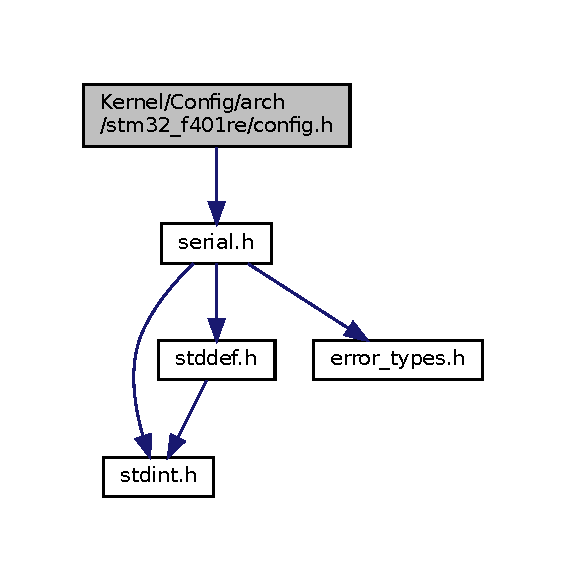
\includegraphics[width=272pt]{config_8h__incl}
\end{center}
\end{figure}
This graph shows which files directly or indirectly include this file\+:\nopagebreak
\begin{figure}[H]
\begin{center}
\leavevmode
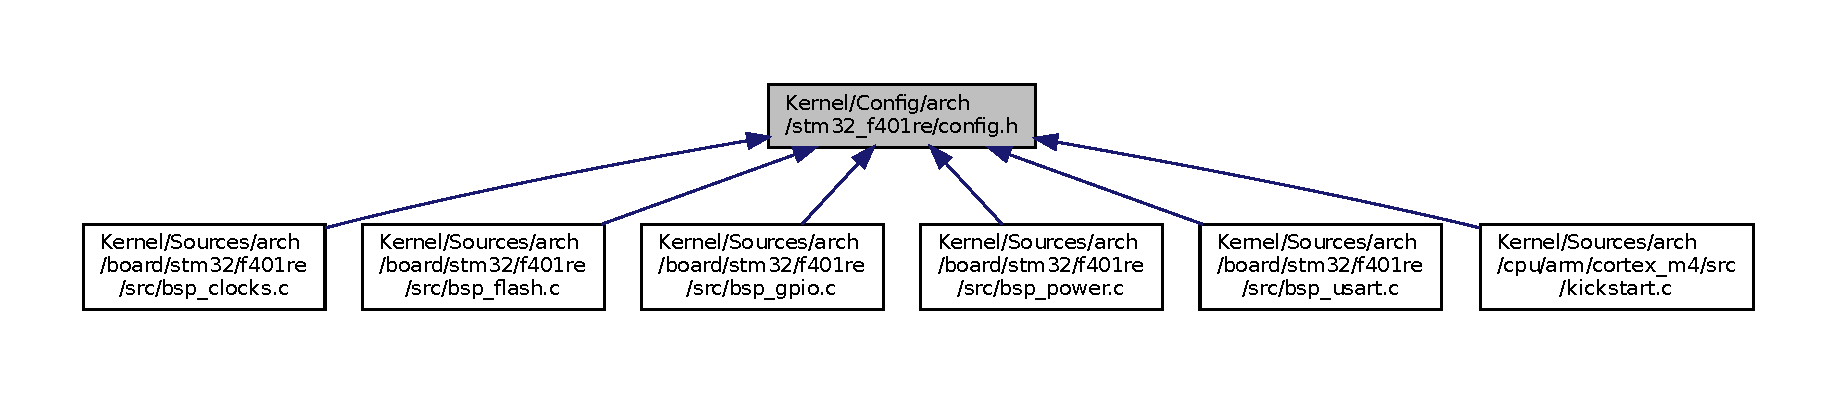
\includegraphics[width=350pt]{config_8h__dep__incl}
\end{center}
\end{figure}
\subsection*{Macros}
\begin{DoxyCompactItemize}
\item 
\#define \hyperlink{config_8h_aadd28d9914163468773660f1142ca822}{C\+O\+N\+F\+I\+G\+\_\+\+U\+A\+R\+T\+\_\+\+S\+E\+T\+T\+I\+N\+GS}
\item 
\#define \hyperlink{config_8h_a023f94f341f2300adee0891b15b364b2}{E\+R\+R\+O\+R\+\_\+\+L\+O\+G\+\_\+\+L\+E\+V\+EL}~3
\item 
\#define \hyperlink{config_8h_ae4ead2e291cd4f0949966eff6513bd20}{W\+A\+R\+N\+I\+N\+G\+\_\+\+L\+O\+G\+\_\+\+L\+E\+V\+EL}~2
\item 
\#define \hyperlink{config_8h_a8fa6c5ec8254575a940cf0a632310a95}{I\+N\+F\+O\+\_\+\+L\+O\+G\+\_\+\+L\+E\+V\+EL}~1
\item 
\#define \hyperlink{config_8h_a76e4c926f6662c7217b7e28510d2fc99}{N\+O\+N\+E\+\_\+\+L\+O\+G\+\_\+\+L\+E\+V\+EL}~0
\item 
\#define \hyperlink{config_8h_a6c272d2b12ffba9bdd5a4d5dd608a0f8}{K\+E\+R\+N\+E\+L\+\_\+\+L\+O\+G\+\_\+\+L\+E\+V\+EL}~\hyperlink{config_8h_a76e4c926f6662c7217b7e28510d2fc99}{N\+O\+N\+E\+\_\+\+L\+O\+G\+\_\+\+L\+E\+V\+EL}
\end{DoxyCompactItemize}


\subsection{Macro Definition Documentation}
\mbox{\Hypertarget{config_8h_aadd28d9914163468773660f1142ca822}\label{config_8h_aadd28d9914163468773660f1142ca822}} 
\index{config.\+h@{config.\+h}!C\+O\+N\+F\+I\+G\+\_\+\+U\+A\+R\+T\+\_\+\+S\+E\+T\+T\+I\+N\+GS@{C\+O\+N\+F\+I\+G\+\_\+\+U\+A\+R\+T\+\_\+\+S\+E\+T\+T\+I\+N\+GS}}
\index{C\+O\+N\+F\+I\+G\+\_\+\+U\+A\+R\+T\+\_\+\+S\+E\+T\+T\+I\+N\+GS@{C\+O\+N\+F\+I\+G\+\_\+\+U\+A\+R\+T\+\_\+\+S\+E\+T\+T\+I\+N\+GS}!config.\+h@{config.\+h}}
\subsubsection{\texorpdfstring{C\+O\+N\+F\+I\+G\+\_\+\+U\+A\+R\+T\+\_\+\+S\+E\+T\+T\+I\+N\+GS}{CONFIG\_UART\_SETTINGS}}
{\footnotesize\ttfamily \#define C\+O\+N\+F\+I\+G\+\_\+\+U\+A\+R\+T\+\_\+\+S\+E\+T\+T\+I\+N\+GS}

{\bfseries Value\+:}
\begin{DoxyCode}
\{                  \(\backslash\)
    .baudrate    = 115200,                      \(\backslash\)
    .word\_length = 8,                           \(\backslash\)
    .stop\_bits   = \hyperlink{serial_8h_a2b63bfe663eaa7e96165898d0bad9ba1}{SERIAL\_STOP\_BITS\_1},          \(\backslash\)
    .partity     = \hyperlink{serial_8h_ad3af92391cfd2670eb782a60c7f923a6}{SERIAL\_PARITY\_NONE},          \(\backslash\)
    .ctrl\_flow   = \hyperlink{serial_8h_ab85f99523d332a127bd78d8fd075e9f4}{SERIAL\_CTRL\_FLOW\_NONE}        \(\backslash\)
\}
\end{DoxyCode}
Kernel\textquotesingle{}s serial settings. 

Definition at line 22 of file config.\+h.

\mbox{\Hypertarget{config_8h_a023f94f341f2300adee0891b15b364b2}\label{config_8h_a023f94f341f2300adee0891b15b364b2}} 
\index{config.\+h@{config.\+h}!E\+R\+R\+O\+R\+\_\+\+L\+O\+G\+\_\+\+L\+E\+V\+EL@{E\+R\+R\+O\+R\+\_\+\+L\+O\+G\+\_\+\+L\+E\+V\+EL}}
\index{E\+R\+R\+O\+R\+\_\+\+L\+O\+G\+\_\+\+L\+E\+V\+EL@{E\+R\+R\+O\+R\+\_\+\+L\+O\+G\+\_\+\+L\+E\+V\+EL}!config.\+h@{config.\+h}}
\subsubsection{\texorpdfstring{E\+R\+R\+O\+R\+\_\+\+L\+O\+G\+\_\+\+L\+E\+V\+EL}{ERROR\_LOG\_LEVEL}}
{\footnotesize\ttfamily \#define E\+R\+R\+O\+R\+\_\+\+L\+O\+G\+\_\+\+L\+E\+V\+EL~3}



Definition at line 31 of file config.\+h.

\mbox{\Hypertarget{config_8h_a8fa6c5ec8254575a940cf0a632310a95}\label{config_8h_a8fa6c5ec8254575a940cf0a632310a95}} 
\index{config.\+h@{config.\+h}!I\+N\+F\+O\+\_\+\+L\+O\+G\+\_\+\+L\+E\+V\+EL@{I\+N\+F\+O\+\_\+\+L\+O\+G\+\_\+\+L\+E\+V\+EL}}
\index{I\+N\+F\+O\+\_\+\+L\+O\+G\+\_\+\+L\+E\+V\+EL@{I\+N\+F\+O\+\_\+\+L\+O\+G\+\_\+\+L\+E\+V\+EL}!config.\+h@{config.\+h}}
\subsubsection{\texorpdfstring{I\+N\+F\+O\+\_\+\+L\+O\+G\+\_\+\+L\+E\+V\+EL}{INFO\_LOG\_LEVEL}}
{\footnotesize\ttfamily \#define I\+N\+F\+O\+\_\+\+L\+O\+G\+\_\+\+L\+E\+V\+EL~1}



Definition at line 33 of file config.\+h.

\mbox{\Hypertarget{config_8h_a6c272d2b12ffba9bdd5a4d5dd608a0f8}\label{config_8h_a6c272d2b12ffba9bdd5a4d5dd608a0f8}} 
\index{config.\+h@{config.\+h}!K\+E\+R\+N\+E\+L\+\_\+\+L\+O\+G\+\_\+\+L\+E\+V\+EL@{K\+E\+R\+N\+E\+L\+\_\+\+L\+O\+G\+\_\+\+L\+E\+V\+EL}}
\index{K\+E\+R\+N\+E\+L\+\_\+\+L\+O\+G\+\_\+\+L\+E\+V\+EL@{K\+E\+R\+N\+E\+L\+\_\+\+L\+O\+G\+\_\+\+L\+E\+V\+EL}!config.\+h@{config.\+h}}
\subsubsection{\texorpdfstring{K\+E\+R\+N\+E\+L\+\_\+\+L\+O\+G\+\_\+\+L\+E\+V\+EL}{KERNEL\_LOG\_LEVEL}}
{\footnotesize\ttfamily \#define K\+E\+R\+N\+E\+L\+\_\+\+L\+O\+G\+\_\+\+L\+E\+V\+EL~\hyperlink{config_8h_a76e4c926f6662c7217b7e28510d2fc99}{N\+O\+N\+E\+\_\+\+L\+O\+G\+\_\+\+L\+E\+V\+EL}}



Definition at line 36 of file config.\+h.

\mbox{\Hypertarget{config_8h_a76e4c926f6662c7217b7e28510d2fc99}\label{config_8h_a76e4c926f6662c7217b7e28510d2fc99}} 
\index{config.\+h@{config.\+h}!N\+O\+N\+E\+\_\+\+L\+O\+G\+\_\+\+L\+E\+V\+EL@{N\+O\+N\+E\+\_\+\+L\+O\+G\+\_\+\+L\+E\+V\+EL}}
\index{N\+O\+N\+E\+\_\+\+L\+O\+G\+\_\+\+L\+E\+V\+EL@{N\+O\+N\+E\+\_\+\+L\+O\+G\+\_\+\+L\+E\+V\+EL}!config.\+h@{config.\+h}}
\subsubsection{\texorpdfstring{N\+O\+N\+E\+\_\+\+L\+O\+G\+\_\+\+L\+E\+V\+EL}{NONE\_LOG\_LEVEL}}
{\footnotesize\ttfamily \#define N\+O\+N\+E\+\_\+\+L\+O\+G\+\_\+\+L\+E\+V\+EL~0}



Definition at line 34 of file config.\+h.

\mbox{\Hypertarget{config_8h_ae4ead2e291cd4f0949966eff6513bd20}\label{config_8h_ae4ead2e291cd4f0949966eff6513bd20}} 
\index{config.\+h@{config.\+h}!W\+A\+R\+N\+I\+N\+G\+\_\+\+L\+O\+G\+\_\+\+L\+E\+V\+EL@{W\+A\+R\+N\+I\+N\+G\+\_\+\+L\+O\+G\+\_\+\+L\+E\+V\+EL}}
\index{W\+A\+R\+N\+I\+N\+G\+\_\+\+L\+O\+G\+\_\+\+L\+E\+V\+EL@{W\+A\+R\+N\+I\+N\+G\+\_\+\+L\+O\+G\+\_\+\+L\+E\+V\+EL}!config.\+h@{config.\+h}}
\subsubsection{\texorpdfstring{W\+A\+R\+N\+I\+N\+G\+\_\+\+L\+O\+G\+\_\+\+L\+E\+V\+EL}{WARNING\_LOG\_LEVEL}}
{\footnotesize\ttfamily \#define W\+A\+R\+N\+I\+N\+G\+\_\+\+L\+O\+G\+\_\+\+L\+E\+V\+EL~2}



Definition at line 32 of file config.\+h.


\hypertarget{clocks_8h}{}\section{Kernel/\+Sources/arch/board/includes/clocks.h File Reference}
\label{clocks_8h}\index{Kernel/\+Sources/arch/board/includes/clocks.\+h@{Kernel/\+Sources/arch/board/includes/clocks.\+h}}

\hypertarget{serial_8h}{}\section{Kernel/\+Sources/arch/board/includes/serial.h File Reference}
\label{serial_8h}\index{Kernel/\+Sources/arch/board/includes/serial.\+h@{Kernel/\+Sources/arch/board/includes/serial.\+h}}
{\ttfamily \#include \char`\"{}stdint.\+h\char`\"{}}\newline
{\ttfamily \#include \char`\"{}stddef.\+h\char`\"{}}\newline
{\ttfamily \#include \char`\"{}error\+\_\+types.\+h\char`\"{}}\newline
Include dependency graph for serial.\+h\+:\nopagebreak
\begin{figure}[H]
\begin{center}
\leavevmode
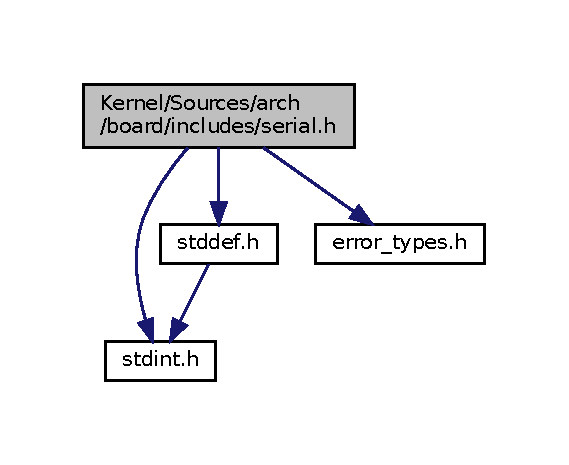
\includegraphics[width=273pt]{serial_8h__incl}
\end{center}
\end{figure}
This graph shows which files directly or indirectly include this file\+:\nopagebreak
\begin{figure}[H]
\begin{center}
\leavevmode
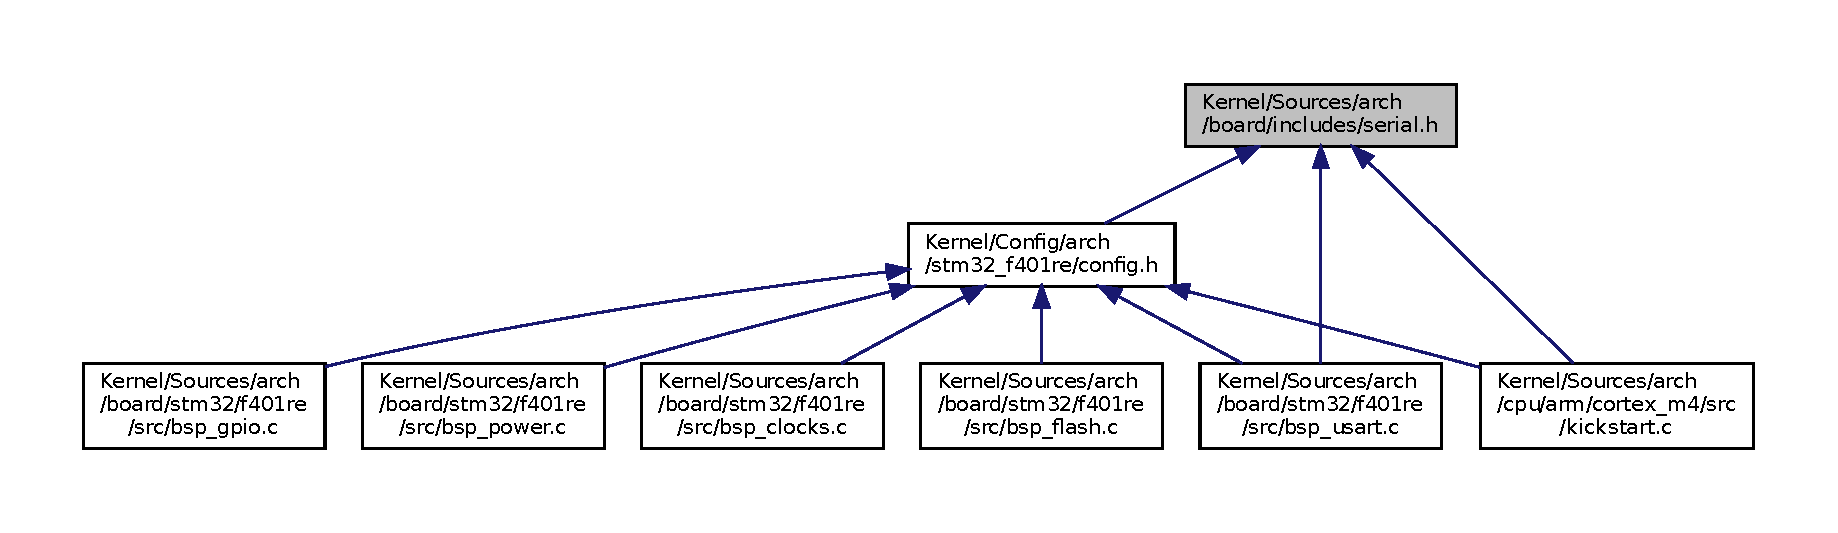
\includegraphics[width=350pt]{serial_8h__dep__incl}
\end{center}
\end{figure}
\subsection*{Data Structures}
\begin{DoxyCompactItemize}
\item 
struct \hyperlink{struct_s_e_r_i_a_l___s_e_t_t_i_n_g_s}{S\+E\+R\+I\+A\+L\+\_\+\+S\+E\+T\+T\+I\+N\+GS}
\begin{DoxyCompactList}\small\item\em Serial settings structure that contains the parameters used to configure the serial line. \end{DoxyCompactList}\end{DoxyCompactItemize}
\subsection*{Macros}
\begin{DoxyCompactItemize}
\item 
\#define \hyperlink{serial_8h_ad3af92391cfd2670eb782a60c7f923a6}{S\+E\+R\+I\+A\+L\+\_\+\+P\+A\+R\+I\+T\+Y\+\_\+\+N\+O\+NE}~0
\begin{DoxyCompactList}\small\item\em Serial parity setting\+: no parity. \end{DoxyCompactList}\item 
\#define \hyperlink{serial_8h_aa1baeda93fe64b888113824d02471d0f}{S\+E\+R\+I\+A\+L\+\_\+\+P\+A\+R\+I\+T\+Y\+\_\+\+O\+DD}~1
\begin{DoxyCompactList}\small\item\em Serial parity setting\+: odd parity. \end{DoxyCompactList}\item 
\#define \hyperlink{serial_8h_ab1469484b1ad5e39561c21b5a590eaf6}{S\+E\+R\+I\+A\+L\+\_\+\+P\+A\+R\+I\+T\+Y\+\_\+\+E\+V\+EN}~2
\begin{DoxyCompactList}\small\item\em Serial parity setting\+: even parity. \end{DoxyCompactList}\item 
\#define \hyperlink{serial_8h_a53a4c884223db0ce40e97ed0cc5e6d19}{S\+E\+R\+I\+A\+L\+\_\+\+S\+T\+O\+P\+\_\+\+B\+I\+T\+S\+\_\+05}~0
\begin{DoxyCompactList}\small\item\em Serial stop bits number\+: 0.\+5 bits. \end{DoxyCompactList}\item 
\#define \hyperlink{serial_8h_a2b63bfe663eaa7e96165898d0bad9ba1}{S\+E\+R\+I\+A\+L\+\_\+\+S\+T\+O\+P\+\_\+\+B\+I\+T\+S\+\_\+1}~1
\begin{DoxyCompactList}\small\item\em Serial stop bits number\+: 1 bits. \end{DoxyCompactList}\item 
\#define \hyperlink{serial_8h_adfe27b7a5b350830ec68973c5aa7de7a}{S\+E\+R\+I\+A\+L\+\_\+\+S\+T\+O\+P\+\_\+\+B\+I\+T\+S\+\_\+15}~2
\begin{DoxyCompactList}\small\item\em Serial stop bits number\+: 1.\+5 bits. \end{DoxyCompactList}\item 
\#define \hyperlink{serial_8h_ad91c5a26785732ceabc6feddf28a2695}{S\+E\+R\+I\+A\+L\+\_\+\+S\+T\+O\+P\+\_\+\+B\+I\+T\+S\+\_\+2}~3
\begin{DoxyCompactList}\small\item\em Serial stop bits number\+: 2 bits. \end{DoxyCompactList}\item 
\#define \hyperlink{serial_8h_ab85f99523d332a127bd78d8fd075e9f4}{S\+E\+R\+I\+A\+L\+\_\+\+C\+T\+R\+L\+\_\+\+F\+L\+O\+W\+\_\+\+N\+O\+NE}~0
\begin{DoxyCompactList}\small\item\em Serial flow control method\+: no control. \end{DoxyCompactList}\item 
\#define \hyperlink{serial_8h_a547310a9a903fa2fe282cb02236a6278}{S\+E\+R\+I\+A\+L\+\_\+\+C\+T\+R\+L\+\_\+\+F\+L\+O\+W\+\_\+\+X\+O\+N\+X\+O\+FF}~1
\begin{DoxyCompactList}\small\item\em Serial flow control method\+: X\+O\+N/\+X\+O\+FF control. \end{DoxyCompactList}\item 
\#define \hyperlink{serial_8h_a0d44b3d3d3e5bb25dc7b976dc2acd4d6}{S\+E\+R\+I\+A\+L\+\_\+\+C\+T\+R\+L\+\_\+\+F\+L\+O\+W\+\_\+\+C\+TS}~2
\begin{DoxyCompactList}\small\item\em Serial flow control method\+: hardware C\+TS control. \end{DoxyCompactList}\item 
\#define \hyperlink{serial_8h_a2335857b5c95b76430e052c05f6e71b5}{S\+E\+R\+I\+A\+L\+\_\+\+C\+T\+R\+L\+\_\+\+F\+L\+O\+W\+\_\+\+R\+TS}~3
\begin{DoxyCompactList}\small\item\em Serial flow control method\+: hardware R\+TS control. \end{DoxyCompactList}\item 
\#define \hyperlink{serial_8h_a5eadb2a7b63f2b5483b5c4aed197d99a}{S\+E\+R\+I\+A\+L\+\_\+\+C\+T\+R\+L\+\_\+\+F\+L\+O\+W\+\_\+\+C\+T\+S\+\_\+\+R\+TS}~4
\begin{DoxyCompactList}\small\item\em Serial flow control method\+: hardware C\+T\+Sand R\+TS control. \end{DoxyCompactList}\end{DoxyCompactItemize}
\subsection*{Typedefs}
\begin{DoxyCompactItemize}
\item 
typedef struct \hyperlink{struct_s_e_r_i_a_l___s_e_t_t_i_n_g_s}{S\+E\+R\+I\+A\+L\+\_\+\+S\+E\+T\+T\+I\+N\+GS} \hyperlink{serial_8h_acf007a933480ae3b580e6bccdc4b7c40}{S\+E\+R\+I\+A\+L\+\_\+\+S\+E\+T\+T\+I\+N\+G\+S\+\_\+T}
\begin{DoxyCompactList}\small\item\em Sharthand for struct \hyperlink{struct_s_e_r_i_a_l___s_e_t_t_i_n_g_s}{S\+E\+R\+I\+A\+L\+\_\+\+S\+E\+T\+T\+I\+N\+GS}. \end{DoxyCompactList}\end{DoxyCompactItemize}
\subsection*{Functions}
\begin{DoxyCompactItemize}
\item 
\hyperlink{error__types_8h_acf146bc98f60f47c79d782f7523e339c}{E\+R\+R\+O\+R\+\_\+\+C\+O\+D\+E\+\_\+E} \hyperlink{serial_8h_ac8063a6773891c77be25ad972f915f35}{serial\+\_\+init} (const \hyperlink{serial_8h_acf007a933480ae3b580e6bccdc4b7c40}{S\+E\+R\+I\+A\+L\+\_\+\+S\+E\+T\+T\+I\+N\+G\+S\+\_\+T} $\ast$settings)
\begin{DoxyCompactList}\small\item\em Initializes the serial line. \end{DoxyCompactList}\item 
\hyperlink{error__types_8h_acf146bc98f60f47c79d782f7523e339c}{E\+R\+R\+O\+R\+\_\+\+C\+O\+D\+E\+\_\+E} \hyperlink{serial_8h_a28c404f87f73ce3d02c889d4792d6a19}{serial\+\_\+write} (const char $\ast$str, const \hyperlink{stddef_8h_aa9d55e2f20e580b7445617d0d12fff6e}{size\+\_\+t} length)
\begin{DoxyCompactList}\small\item\em Writes a string of characters to the serial line. \end{DoxyCompactList}\end{DoxyCompactItemize}


\subsection{Macro Definition Documentation}
\mbox{\Hypertarget{serial_8h_a0d44b3d3d3e5bb25dc7b976dc2acd4d6}\label{serial_8h_a0d44b3d3d3e5bb25dc7b976dc2acd4d6}} 
\index{serial.\+h@{serial.\+h}!S\+E\+R\+I\+A\+L\+\_\+\+C\+T\+R\+L\+\_\+\+F\+L\+O\+W\+\_\+\+C\+TS@{S\+E\+R\+I\+A\+L\+\_\+\+C\+T\+R\+L\+\_\+\+F\+L\+O\+W\+\_\+\+C\+TS}}
\index{S\+E\+R\+I\+A\+L\+\_\+\+C\+T\+R\+L\+\_\+\+F\+L\+O\+W\+\_\+\+C\+TS@{S\+E\+R\+I\+A\+L\+\_\+\+C\+T\+R\+L\+\_\+\+F\+L\+O\+W\+\_\+\+C\+TS}!serial.\+h@{serial.\+h}}
\subsubsection{\texorpdfstring{S\+E\+R\+I\+A\+L\+\_\+\+C\+T\+R\+L\+\_\+\+F\+L\+O\+W\+\_\+\+C\+TS}{SERIAL\_CTRL\_FLOW\_CTS}}
{\footnotesize\ttfamily \#define S\+E\+R\+I\+A\+L\+\_\+\+C\+T\+R\+L\+\_\+\+F\+L\+O\+W\+\_\+\+C\+TS~2}



Serial flow control method\+: hardware C\+TS control. 



Definition at line 48 of file serial.\+h.

\mbox{\Hypertarget{serial_8h_a5eadb2a7b63f2b5483b5c4aed197d99a}\label{serial_8h_a5eadb2a7b63f2b5483b5c4aed197d99a}} 
\index{serial.\+h@{serial.\+h}!S\+E\+R\+I\+A\+L\+\_\+\+C\+T\+R\+L\+\_\+\+F\+L\+O\+W\+\_\+\+C\+T\+S\+\_\+\+R\+TS@{S\+E\+R\+I\+A\+L\+\_\+\+C\+T\+R\+L\+\_\+\+F\+L\+O\+W\+\_\+\+C\+T\+S\+\_\+\+R\+TS}}
\index{S\+E\+R\+I\+A\+L\+\_\+\+C\+T\+R\+L\+\_\+\+F\+L\+O\+W\+\_\+\+C\+T\+S\+\_\+\+R\+TS@{S\+E\+R\+I\+A\+L\+\_\+\+C\+T\+R\+L\+\_\+\+F\+L\+O\+W\+\_\+\+C\+T\+S\+\_\+\+R\+TS}!serial.\+h@{serial.\+h}}
\subsubsection{\texorpdfstring{S\+E\+R\+I\+A\+L\+\_\+\+C\+T\+R\+L\+\_\+\+F\+L\+O\+W\+\_\+\+C\+T\+S\+\_\+\+R\+TS}{SERIAL\_CTRL\_FLOW\_CTS\_RTS}}
{\footnotesize\ttfamily \#define S\+E\+R\+I\+A\+L\+\_\+\+C\+T\+R\+L\+\_\+\+F\+L\+O\+W\+\_\+\+C\+T\+S\+\_\+\+R\+TS~4}



Serial flow control method\+: hardware C\+T\+Sand R\+TS control. 



Definition at line 52 of file serial.\+h.

\mbox{\Hypertarget{serial_8h_ab85f99523d332a127bd78d8fd075e9f4}\label{serial_8h_ab85f99523d332a127bd78d8fd075e9f4}} 
\index{serial.\+h@{serial.\+h}!S\+E\+R\+I\+A\+L\+\_\+\+C\+T\+R\+L\+\_\+\+F\+L\+O\+W\+\_\+\+N\+O\+NE@{S\+E\+R\+I\+A\+L\+\_\+\+C\+T\+R\+L\+\_\+\+F\+L\+O\+W\+\_\+\+N\+O\+NE}}
\index{S\+E\+R\+I\+A\+L\+\_\+\+C\+T\+R\+L\+\_\+\+F\+L\+O\+W\+\_\+\+N\+O\+NE@{S\+E\+R\+I\+A\+L\+\_\+\+C\+T\+R\+L\+\_\+\+F\+L\+O\+W\+\_\+\+N\+O\+NE}!serial.\+h@{serial.\+h}}
\subsubsection{\texorpdfstring{S\+E\+R\+I\+A\+L\+\_\+\+C\+T\+R\+L\+\_\+\+F\+L\+O\+W\+\_\+\+N\+O\+NE}{SERIAL\_CTRL\_FLOW\_NONE}}
{\footnotesize\ttfamily \#define S\+E\+R\+I\+A\+L\+\_\+\+C\+T\+R\+L\+\_\+\+F\+L\+O\+W\+\_\+\+N\+O\+NE~0}



Serial flow control method\+: no control. 



Definition at line 44 of file serial.\+h.

\mbox{\Hypertarget{serial_8h_a2335857b5c95b76430e052c05f6e71b5}\label{serial_8h_a2335857b5c95b76430e052c05f6e71b5}} 
\index{serial.\+h@{serial.\+h}!S\+E\+R\+I\+A\+L\+\_\+\+C\+T\+R\+L\+\_\+\+F\+L\+O\+W\+\_\+\+R\+TS@{S\+E\+R\+I\+A\+L\+\_\+\+C\+T\+R\+L\+\_\+\+F\+L\+O\+W\+\_\+\+R\+TS}}
\index{S\+E\+R\+I\+A\+L\+\_\+\+C\+T\+R\+L\+\_\+\+F\+L\+O\+W\+\_\+\+R\+TS@{S\+E\+R\+I\+A\+L\+\_\+\+C\+T\+R\+L\+\_\+\+F\+L\+O\+W\+\_\+\+R\+TS}!serial.\+h@{serial.\+h}}
\subsubsection{\texorpdfstring{S\+E\+R\+I\+A\+L\+\_\+\+C\+T\+R\+L\+\_\+\+F\+L\+O\+W\+\_\+\+R\+TS}{SERIAL\_CTRL\_FLOW\_RTS}}
{\footnotesize\ttfamily \#define S\+E\+R\+I\+A\+L\+\_\+\+C\+T\+R\+L\+\_\+\+F\+L\+O\+W\+\_\+\+R\+TS~3}



Serial flow control method\+: hardware R\+TS control. 



Definition at line 50 of file serial.\+h.

\mbox{\Hypertarget{serial_8h_a547310a9a903fa2fe282cb02236a6278}\label{serial_8h_a547310a9a903fa2fe282cb02236a6278}} 
\index{serial.\+h@{serial.\+h}!S\+E\+R\+I\+A\+L\+\_\+\+C\+T\+R\+L\+\_\+\+F\+L\+O\+W\+\_\+\+X\+O\+N\+X\+O\+FF@{S\+E\+R\+I\+A\+L\+\_\+\+C\+T\+R\+L\+\_\+\+F\+L\+O\+W\+\_\+\+X\+O\+N\+X\+O\+FF}}
\index{S\+E\+R\+I\+A\+L\+\_\+\+C\+T\+R\+L\+\_\+\+F\+L\+O\+W\+\_\+\+X\+O\+N\+X\+O\+FF@{S\+E\+R\+I\+A\+L\+\_\+\+C\+T\+R\+L\+\_\+\+F\+L\+O\+W\+\_\+\+X\+O\+N\+X\+O\+FF}!serial.\+h@{serial.\+h}}
\subsubsection{\texorpdfstring{S\+E\+R\+I\+A\+L\+\_\+\+C\+T\+R\+L\+\_\+\+F\+L\+O\+W\+\_\+\+X\+O\+N\+X\+O\+FF}{SERIAL\_CTRL\_FLOW\_XONXOFF}}
{\footnotesize\ttfamily \#define S\+E\+R\+I\+A\+L\+\_\+\+C\+T\+R\+L\+\_\+\+F\+L\+O\+W\+\_\+\+X\+O\+N\+X\+O\+FF~1}



Serial flow control method\+: X\+O\+N/\+X\+O\+FF control. 



Definition at line 46 of file serial.\+h.

\mbox{\Hypertarget{serial_8h_ab1469484b1ad5e39561c21b5a590eaf6}\label{serial_8h_ab1469484b1ad5e39561c21b5a590eaf6}} 
\index{serial.\+h@{serial.\+h}!S\+E\+R\+I\+A\+L\+\_\+\+P\+A\+R\+I\+T\+Y\+\_\+\+E\+V\+EN@{S\+E\+R\+I\+A\+L\+\_\+\+P\+A\+R\+I\+T\+Y\+\_\+\+E\+V\+EN}}
\index{S\+E\+R\+I\+A\+L\+\_\+\+P\+A\+R\+I\+T\+Y\+\_\+\+E\+V\+EN@{S\+E\+R\+I\+A\+L\+\_\+\+P\+A\+R\+I\+T\+Y\+\_\+\+E\+V\+EN}!serial.\+h@{serial.\+h}}
\subsubsection{\texorpdfstring{S\+E\+R\+I\+A\+L\+\_\+\+P\+A\+R\+I\+T\+Y\+\_\+\+E\+V\+EN}{SERIAL\_PARITY\_EVEN}}
{\footnotesize\ttfamily \#define S\+E\+R\+I\+A\+L\+\_\+\+P\+A\+R\+I\+T\+Y\+\_\+\+E\+V\+EN~2}



Serial parity setting\+: even parity. 



Definition at line 32 of file serial.\+h.

\mbox{\Hypertarget{serial_8h_ad3af92391cfd2670eb782a60c7f923a6}\label{serial_8h_ad3af92391cfd2670eb782a60c7f923a6}} 
\index{serial.\+h@{serial.\+h}!S\+E\+R\+I\+A\+L\+\_\+\+P\+A\+R\+I\+T\+Y\+\_\+\+N\+O\+NE@{S\+E\+R\+I\+A\+L\+\_\+\+P\+A\+R\+I\+T\+Y\+\_\+\+N\+O\+NE}}
\index{S\+E\+R\+I\+A\+L\+\_\+\+P\+A\+R\+I\+T\+Y\+\_\+\+N\+O\+NE@{S\+E\+R\+I\+A\+L\+\_\+\+P\+A\+R\+I\+T\+Y\+\_\+\+N\+O\+NE}!serial.\+h@{serial.\+h}}
\subsubsection{\texorpdfstring{S\+E\+R\+I\+A\+L\+\_\+\+P\+A\+R\+I\+T\+Y\+\_\+\+N\+O\+NE}{SERIAL\_PARITY\_NONE}}
{\footnotesize\ttfamily \#define S\+E\+R\+I\+A\+L\+\_\+\+P\+A\+R\+I\+T\+Y\+\_\+\+N\+O\+NE~0}



Serial parity setting\+: no parity. 



Definition at line 28 of file serial.\+h.

\mbox{\Hypertarget{serial_8h_aa1baeda93fe64b888113824d02471d0f}\label{serial_8h_aa1baeda93fe64b888113824d02471d0f}} 
\index{serial.\+h@{serial.\+h}!S\+E\+R\+I\+A\+L\+\_\+\+P\+A\+R\+I\+T\+Y\+\_\+\+O\+DD@{S\+E\+R\+I\+A\+L\+\_\+\+P\+A\+R\+I\+T\+Y\+\_\+\+O\+DD}}
\index{S\+E\+R\+I\+A\+L\+\_\+\+P\+A\+R\+I\+T\+Y\+\_\+\+O\+DD@{S\+E\+R\+I\+A\+L\+\_\+\+P\+A\+R\+I\+T\+Y\+\_\+\+O\+DD}!serial.\+h@{serial.\+h}}
\subsubsection{\texorpdfstring{S\+E\+R\+I\+A\+L\+\_\+\+P\+A\+R\+I\+T\+Y\+\_\+\+O\+DD}{SERIAL\_PARITY\_ODD}}
{\footnotesize\ttfamily \#define S\+E\+R\+I\+A\+L\+\_\+\+P\+A\+R\+I\+T\+Y\+\_\+\+O\+DD~1}



Serial parity setting\+: odd parity. 



Definition at line 30 of file serial.\+h.

\mbox{\Hypertarget{serial_8h_a53a4c884223db0ce40e97ed0cc5e6d19}\label{serial_8h_a53a4c884223db0ce40e97ed0cc5e6d19}} 
\index{serial.\+h@{serial.\+h}!S\+E\+R\+I\+A\+L\+\_\+\+S\+T\+O\+P\+\_\+\+B\+I\+T\+S\+\_\+05@{S\+E\+R\+I\+A\+L\+\_\+\+S\+T\+O\+P\+\_\+\+B\+I\+T\+S\+\_\+05}}
\index{S\+E\+R\+I\+A\+L\+\_\+\+S\+T\+O\+P\+\_\+\+B\+I\+T\+S\+\_\+05@{S\+E\+R\+I\+A\+L\+\_\+\+S\+T\+O\+P\+\_\+\+B\+I\+T\+S\+\_\+05}!serial.\+h@{serial.\+h}}
\subsubsection{\texorpdfstring{S\+E\+R\+I\+A\+L\+\_\+\+S\+T\+O\+P\+\_\+\+B\+I\+T\+S\+\_\+05}{SERIAL\_STOP\_BITS\_05}}
{\footnotesize\ttfamily \#define S\+E\+R\+I\+A\+L\+\_\+\+S\+T\+O\+P\+\_\+\+B\+I\+T\+S\+\_\+05~0}



Serial stop bits number\+: 0.\+5 bits. 



Definition at line 35 of file serial.\+h.

\mbox{\Hypertarget{serial_8h_a2b63bfe663eaa7e96165898d0bad9ba1}\label{serial_8h_a2b63bfe663eaa7e96165898d0bad9ba1}} 
\index{serial.\+h@{serial.\+h}!S\+E\+R\+I\+A\+L\+\_\+\+S\+T\+O\+P\+\_\+\+B\+I\+T\+S\+\_\+1@{S\+E\+R\+I\+A\+L\+\_\+\+S\+T\+O\+P\+\_\+\+B\+I\+T\+S\+\_\+1}}
\index{S\+E\+R\+I\+A\+L\+\_\+\+S\+T\+O\+P\+\_\+\+B\+I\+T\+S\+\_\+1@{S\+E\+R\+I\+A\+L\+\_\+\+S\+T\+O\+P\+\_\+\+B\+I\+T\+S\+\_\+1}!serial.\+h@{serial.\+h}}
\subsubsection{\texorpdfstring{S\+E\+R\+I\+A\+L\+\_\+\+S\+T\+O\+P\+\_\+\+B\+I\+T\+S\+\_\+1}{SERIAL\_STOP\_BITS\_1}}
{\footnotesize\ttfamily \#define S\+E\+R\+I\+A\+L\+\_\+\+S\+T\+O\+P\+\_\+\+B\+I\+T\+S\+\_\+1~1}



Serial stop bits number\+: 1 bits. 



Definition at line 37 of file serial.\+h.

\mbox{\Hypertarget{serial_8h_adfe27b7a5b350830ec68973c5aa7de7a}\label{serial_8h_adfe27b7a5b350830ec68973c5aa7de7a}} 
\index{serial.\+h@{serial.\+h}!S\+E\+R\+I\+A\+L\+\_\+\+S\+T\+O\+P\+\_\+\+B\+I\+T\+S\+\_\+15@{S\+E\+R\+I\+A\+L\+\_\+\+S\+T\+O\+P\+\_\+\+B\+I\+T\+S\+\_\+15}}
\index{S\+E\+R\+I\+A\+L\+\_\+\+S\+T\+O\+P\+\_\+\+B\+I\+T\+S\+\_\+15@{S\+E\+R\+I\+A\+L\+\_\+\+S\+T\+O\+P\+\_\+\+B\+I\+T\+S\+\_\+15}!serial.\+h@{serial.\+h}}
\subsubsection{\texorpdfstring{S\+E\+R\+I\+A\+L\+\_\+\+S\+T\+O\+P\+\_\+\+B\+I\+T\+S\+\_\+15}{SERIAL\_STOP\_BITS\_15}}
{\footnotesize\ttfamily \#define S\+E\+R\+I\+A\+L\+\_\+\+S\+T\+O\+P\+\_\+\+B\+I\+T\+S\+\_\+15~2}



Serial stop bits number\+: 1.\+5 bits. 



Definition at line 39 of file serial.\+h.

\mbox{\Hypertarget{serial_8h_ad91c5a26785732ceabc6feddf28a2695}\label{serial_8h_ad91c5a26785732ceabc6feddf28a2695}} 
\index{serial.\+h@{serial.\+h}!S\+E\+R\+I\+A\+L\+\_\+\+S\+T\+O\+P\+\_\+\+B\+I\+T\+S\+\_\+2@{S\+E\+R\+I\+A\+L\+\_\+\+S\+T\+O\+P\+\_\+\+B\+I\+T\+S\+\_\+2}}
\index{S\+E\+R\+I\+A\+L\+\_\+\+S\+T\+O\+P\+\_\+\+B\+I\+T\+S\+\_\+2@{S\+E\+R\+I\+A\+L\+\_\+\+S\+T\+O\+P\+\_\+\+B\+I\+T\+S\+\_\+2}!serial.\+h@{serial.\+h}}
\subsubsection{\texorpdfstring{S\+E\+R\+I\+A\+L\+\_\+\+S\+T\+O\+P\+\_\+\+B\+I\+T\+S\+\_\+2}{SERIAL\_STOP\_BITS\_2}}
{\footnotesize\ttfamily \#define S\+E\+R\+I\+A\+L\+\_\+\+S\+T\+O\+P\+\_\+\+B\+I\+T\+S\+\_\+2~3}



Serial stop bits number\+: 2 bits. 



Definition at line 41 of file serial.\+h.



\subsection{Typedef Documentation}
\mbox{\Hypertarget{serial_8h_acf007a933480ae3b580e6bccdc4b7c40}\label{serial_8h_acf007a933480ae3b580e6bccdc4b7c40}} 
\index{serial.\+h@{serial.\+h}!S\+E\+R\+I\+A\+L\+\_\+\+S\+E\+T\+T\+I\+N\+G\+S\+\_\+T@{S\+E\+R\+I\+A\+L\+\_\+\+S\+E\+T\+T\+I\+N\+G\+S\+\_\+T}}
\index{S\+E\+R\+I\+A\+L\+\_\+\+S\+E\+T\+T\+I\+N\+G\+S\+\_\+T@{S\+E\+R\+I\+A\+L\+\_\+\+S\+E\+T\+T\+I\+N\+G\+S\+\_\+T}!serial.\+h@{serial.\+h}}
\subsubsection{\texorpdfstring{S\+E\+R\+I\+A\+L\+\_\+\+S\+E\+T\+T\+I\+N\+G\+S\+\_\+T}{SERIAL\_SETTINGS\_T}}
{\footnotesize\ttfamily typedef struct \hyperlink{struct_s_e_r_i_a_l___s_e_t_t_i_n_g_s}{S\+E\+R\+I\+A\+L\+\_\+\+S\+E\+T\+T\+I\+N\+GS} \hyperlink{serial_8h_acf007a933480ae3b580e6bccdc4b7c40}{S\+E\+R\+I\+A\+L\+\_\+\+S\+E\+T\+T\+I\+N\+G\+S\+\_\+T}}



Sharthand for struct \hyperlink{struct_s_e_r_i_a_l___s_e_t_t_i_n_g_s}{S\+E\+R\+I\+A\+L\+\_\+\+S\+E\+T\+T\+I\+N\+GS}. 



Definition at line 76 of file serial.\+h.



\subsection{Function Documentation}
\mbox{\Hypertarget{serial_8h_ac8063a6773891c77be25ad972f915f35}\label{serial_8h_ac8063a6773891c77be25ad972f915f35}} 
\index{serial.\+h@{serial.\+h}!serial\+\_\+init@{serial\+\_\+init}}
\index{serial\+\_\+init@{serial\+\_\+init}!serial.\+h@{serial.\+h}}
\subsubsection{\texorpdfstring{serial\+\_\+init()}{serial\_init()}}
{\footnotesize\ttfamily \hyperlink{error__types_8h_acf146bc98f60f47c79d782f7523e339c}{E\+R\+R\+O\+R\+\_\+\+C\+O\+D\+E\+\_\+E} serial\+\_\+init (\begin{DoxyParamCaption}\item[{const \hyperlink{serial_8h_acf007a933480ae3b580e6bccdc4b7c40}{S\+E\+R\+I\+A\+L\+\_\+\+S\+E\+T\+T\+I\+N\+G\+S\+\_\+T} $\ast$}]{settings }\end{DoxyParamCaption})}



Initializes the serial line. 

Initializes the system\textquotesingle{}s serial line. The settings structure is used to set the line\textquotesingle{}s parameter according to th user\textquotesingle{}s choice.


\begin{DoxyParams}[1]{Parameters}
\mbox{\tt in}  & {\em settings} & The settings structure used to initialize the serial line.\\
\hline
\end{DoxyParams}
\begin{DoxyReturn}{Returns}
N\+O\+\_\+\+E\+R\+R\+OR is returned in case of success. Otherwise an error code is returned. Please refer to the list of the standard error codes. 
\end{DoxyReturn}
This function uses U\+S\+A\+R\+T2 as main U\+A\+RT output.

Definition at line 406 of file bsp\+\_\+usart.\+c.


\begin{DoxyCode}
407 \{
411 
412     \hyperlink{struct_g_p_i_o___s_e_t_t_i_n_g_s}{GPIO\_SETTINGS\_T} gpio\_settings;
413     \hyperlink{error__types_8h_acf146bc98f60f47c79d782f7523e339c}{ERROR\_CODE\_E}    error;
414 
415     \textcolor{keywordflow}{if}(\hyperlink{bsp__usart_8c_ad317e99f056e9ce535815fcdd1697c93}{usart\_init\_state} != 0)
416     \{
417 \textcolor{preprocessor}{#if KERNEL\_LOG\_LEVEL == ERROR\_LOG\_LEVEL
}
418         \hyperlink{logger_8h_a580bb63c1418b2fc8456f9b6c5b6d39d}{KERNEL\_LOG\_ERROR}(\textcolor{stringliteral}{"Serial already initialized"}, 
419                          \hyperlink{error__types_8h_a4db9ee29f2ff83c71567c12f6bfbf28ca9af911a6ba1c32ce22213d689cb59f86}{ERROR\_ALREADY\_INIT}, 
420                          \textcolor{keyword}{sizeof}(\hyperlink{error__types_8h_a4db9ee29f2ff83c71567c12f6bfbf28ca9af911a6ba1c32ce22213d689cb59f86}{ERROR\_ALREADY\_INIT}), 
421                          \hyperlink{error__types_8h_a4db9ee29f2ff83c71567c12f6bfbf28ca9af911a6ba1c32ce22213d689cb59f86}{ERROR\_ALREADY\_INIT});
422 \textcolor{preprocessor}{#endif        
}
423         \textcolor{keywordflow}{return} \hyperlink{error__types_8h_a4db9ee29f2ff83c71567c12f6bfbf28ca9af911a6ba1c32ce22213d689cb59f86}{ERROR\_ALREADY\_INIT};
424     \}
425 
426     \textcolor{comment}{/* Check parameters */}
427     \textcolor{keywordflow}{if}(settings == \hyperlink{stddef_8h_a070d2ce7b6bb7e5c05602aa8c308d0c4}{NULL})
428     \{
429 \textcolor{preprocessor}{#if KERNEL\_LOG\_LEVEL == ERROR\_LOG\_LEVEL
}
430         \hyperlink{logger_8h_a580bb63c1418b2fc8456f9b6c5b6d39d}{KERNEL\_LOG\_ERROR}(\textcolor{stringliteral}{"Serial settings structure is NULL"}, 
431                          \hyperlink{error__types_8h_a4db9ee29f2ff83c71567c12f6bfbf28ca3d37cbe00af5e55b2ab0cfac2a5b4b0e}{ERROR\_NULL\_POINTER}, 
432                          \textcolor{keyword}{sizeof}(\hyperlink{error__types_8h_a4db9ee29f2ff83c71567c12f6bfbf28ca3d37cbe00af5e55b2ab0cfac2a5b4b0e}{ERROR\_NULL\_POINTER}), 
433                          \hyperlink{error__types_8h_a4db9ee29f2ff83c71567c12f6bfbf28ca3d37cbe00af5e55b2ab0cfac2a5b4b0e}{ERROR\_NULL\_POINTER});
434 \textcolor{preprocessor}{#endif
}
435         \textcolor{keywordflow}{return} \hyperlink{error__types_8h_a4db9ee29f2ff83c71567c12f6bfbf28ca3d37cbe00af5e55b2ab0cfac2a5b4b0e}{ERROR\_NULL\_POINTER};
436     \}
437     \hyperlink{bsp__usart_8c_a8aa979774d50a01cae417a899595055c}{CHECK\_BAUDRATE}(settings->\hyperlink{struct_s_e_r_i_a_l___s_e_t_t_i_n_g_s_ac4f06ea26ed6bd7ae83b92d64ac10b78}{baudrate});
438     \hyperlink{bsp__usart_8c_a51885194f22c4bd5f94ab0bb253dd079}{CHECK\_WDLENGTH}(settings->\hyperlink{struct_s_e_r_i_a_l___s_e_t_t_i_n_g_s_ae9ff0fba282a81e6b05a1082ab54e14d}{word\_length});
439     \hyperlink{bsp__usart_8c_ace359bfb3e864f995667f829a5520105}{CHECK\_STOPBITS}(settings->\hyperlink{struct_s_e_r_i_a_l___s_e_t_t_i_n_g_s_ae847d8b7e1095e0ae8d6eb1e4a281585}{stop\_bits});
440     \hyperlink{bsp__usart_8c_a2c164787cf0d531b3c026aa2b9193a2b}{CHECK\_PARITYVA}(settings->\hyperlink{struct_s_e_r_i_a_l___s_e_t_t_i_n_g_s_a57fc780fe7a58343cb0513fd873e95fb}{partity});
441     \hyperlink{bsp__usart_8c_a47ca255399a13357557641c6af83af64}{CHECK\_CTRLFLOW}(settings->\hyperlink{struct_s_e_r_i_a_l___s_e_t_t_i_n_g_s_a6f2a9d6a71d9ca705cf561f08e4e222c}{ctrl\_flow});
442 
443     \textcolor{comment}{/* Init GPIO and USART clock */}
444     error = \hyperlink{bsp__clocks_8h_a500b2e77b70c93b3f2b4a94cc9bcf79d}{bsp\_clk\_gpio\_enable}(\hyperlink{bsp__gpio_8h_a69f521b579d2c761dd65949f2bae88f3a4cb73b98ec508807d984052a1598950a}{GPIO\_ID\_A});
445     \textcolor{keywordflow}{if}(error != \hyperlink{error__types_8h_a4db9ee29f2ff83c71567c12f6bfbf28cabf350750d0d4fabd8954c0f1e9bbae94}{NO\_ERROR})
446     \{
447         \textcolor{keywordflow}{return} error;
448     \}
449     error = \hyperlink{bsp__clocks_8h_aaf01af602e17579af5e6af009ae7a557}{bsp\_clk\_usart\_enable}(\hyperlink{bsp__usart_8h_a58f9be3820e29e0fbf00e2466c3ee768abb138542d801249fd01ec62c34f52cff}{USART\_ID\_2});
450     \textcolor{keywordflow}{if}(error != \hyperlink{error__types_8h_a4db9ee29f2ff83c71567c12f6bfbf28cabf350750d0d4fabd8954c0f1e9bbae94}{NO\_ERROR})
451     \{
452         \textcolor{keywordflow}{return} error;
453     \}
454 
455     \textcolor{comment}{/* Initialize the USART2 GPIO A */}
456     gpio\_settings.\hyperlink{struct_g_p_i_o___s_e_t_t_i_n_g_s_aad1e743ccf6e6bc276e61f9ba35bdfd0}{io\_pin}      = \hyperlink{bsp__gpio_8h_a6eee38b797a7268f04357dfa2759efd2}{GPIO\_PIN\_2} | 
457                                 \hyperlink{bsp__gpio_8h_adcaf899c018a0dde572b5af783565c62}{GPIO\_PIN\_3};
458     gpio\_settings.\hyperlink{struct_g_p_i_o___s_e_t_t_i_n_g_s_aca4ea33051d3d932467e31db14e636aa}{io\_modetype} = \hyperlink{bsp__gpio_8h_ae0c591139910f3313c998fdcf74a2b77}{GPIO\_MODE\_ALTFUN}   | 
459                                 \hyperlink{bsp__gpio_8h_af9c9aabc72e4bda42794979584908a8c}{GPIO\_TYPE\_PUSHPULL} | 
460                                 \hyperlink{bsp__gpio_8h_ad53ebddfcc3973120b1c0271423f131e}{GPIO\_PUPD\_NONE};
461     gpio\_settings.\hyperlink{struct_g_p_i_o___s_e_t_t_i_n_g_s_a4555d90ee383bdb9bf2fc3b049f32fd1}{io\_altfunc}  = \hyperlink{bsp__gpio_8h_a6af3869309b2bfedca84f57a7772ee4d}{GPIO\_ALFUNC\_7};
462     gpio\_settings.\hyperlink{struct_g_p_i_o___s_e_t_t_i_n_g_s_aee8d1e0b4f18b0a599ebcbc2e0c8b60f}{io\_speed}    = \hyperlink{bsp__gpio_8h_ae11603e44b5bb26398c583a2410cafd5}{GPIO\_SPEED\_VERY\_HIGH};
463 
464     error = \hyperlink{bsp__gpio_8h_ac05d93f29cf8cdcd3809298fe5df2f87}{bsp\_gpio\_init}(\hyperlink{bsp__gpio_8h_a69f521b579d2c761dd65949f2bae88f3a4cb73b98ec508807d984052a1598950a}{GPIO\_ID\_A}, &gpio\_settings);
465     \textcolor{keywordflow}{if}(error != \hyperlink{error__types_8h_a4db9ee29f2ff83c71567c12f6bfbf28cabf350750d0d4fabd8954c0f1e9bbae94}{NO\_ERROR})
466     \{
467         \textcolor{keywordflow}{return} error;
468     \}
469 
470     \textcolor{comment}{/* Make sure USART2 is disabled */}
471     \hyperlink{bsp__usart_8c_a81aa58ca3b3ff2a16c5666f1601dedc7}{bsp\_usart\_disable}(\hyperlink{bsp__usart_8h_a58f9be3820e29e0fbf00e2466c3ee768abb138542d801249fd01ec62c34f52cff}{USART\_ID\_2});
472 
473     \textcolor{comment}{/* Set USART2 settings */}
474     \hyperlink{bsp__usart_8c_a39d14fff7f007d639de7a6db12fd8acf}{bsp\_uart\_init}(\hyperlink{bsp__usart_8h_a58f9be3820e29e0fbf00e2466c3ee768abb138542d801249fd01ec62c34f52cff}{USART\_ID\_2}, settings);
475 
476     \textcolor{comment}{/* Enable USART2 */}
477     \hyperlink{bsp__usart_8c_ae71596fd1683989728deee59105b9b06}{bsp\_usart\_enable}(\hyperlink{bsp__usart_8h_a58f9be3820e29e0fbf00e2466c3ee768abb138542d801249fd01ec62c34f52cff}{USART\_ID\_2});
478 
479 \textcolor{preprocessor}{#if KERNEL\_LOG\_LEVEL >= INFO\_LOG\_LEVEL
}
480     KERNEL\_LOG\_INFO(\textcolor{stringliteral}{"USART initialized"}, 
481                      \hyperlink{error__types_8h_a4db9ee29f2ff83c71567c12f6bfbf28cabf350750d0d4fabd8954c0f1e9bbae94}{NO\_ERROR}, 
482                      \textcolor{keyword}{sizeof}(\hyperlink{error__types_8h_a4db9ee29f2ff83c71567c12f6bfbf28cabf350750d0d4fabd8954c0f1e9bbae94}{NO\_ERROR}), 
483                      \hyperlink{error__types_8h_a4db9ee29f2ff83c71567c12f6bfbf28cabf350750d0d4fabd8954c0f1e9bbae94}{NO\_ERROR});
484 \textcolor{preprocessor}{#endif 
}
485     \hyperlink{bsp__usart_8c_ad317e99f056e9ce535815fcdd1697c93}{usart\_init\_state} = 1;
486     \textcolor{keywordflow}{return} \hyperlink{error__types_8h_a4db9ee29f2ff83c71567c12f6bfbf28cabf350750d0d4fabd8954c0f1e9bbae94}{NO\_ERROR};
487 \}
\end{DoxyCode}
Here is the call graph for this function\+:
\nopagebreak
\begin{figure}[H]
\begin{center}
\leavevmode
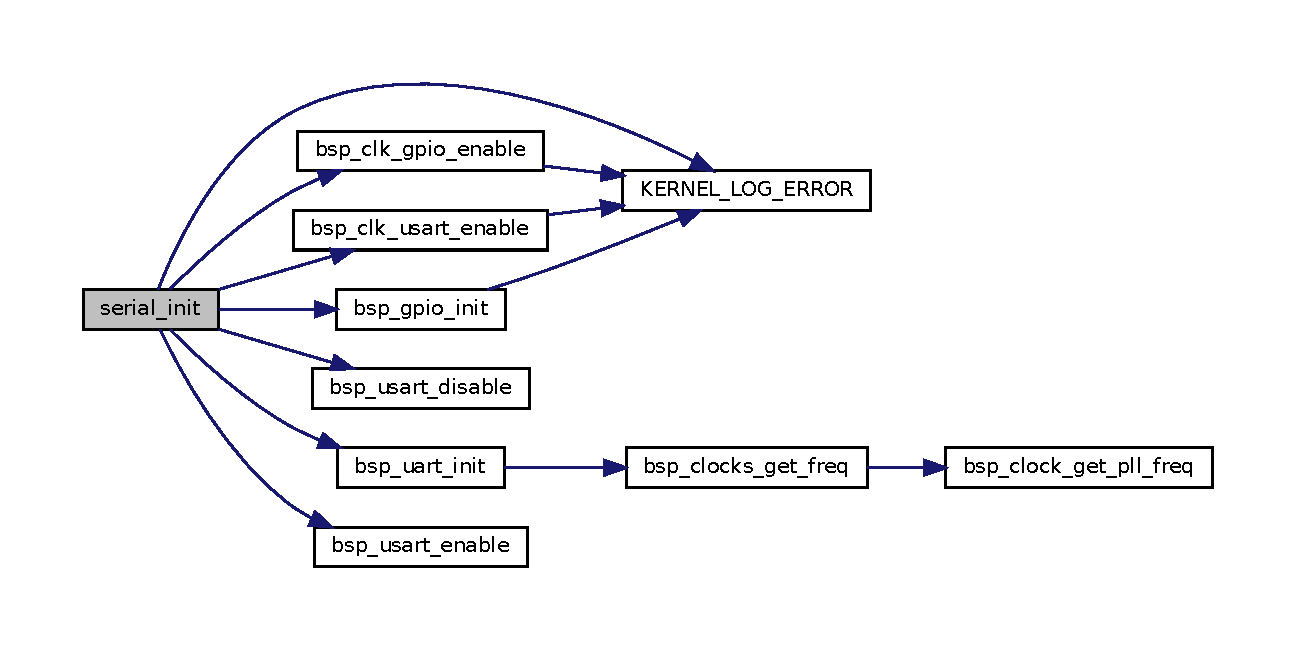
\includegraphics[width=350pt]{serial_8h_ac8063a6773891c77be25ad972f915f35_cgraph}
\end{center}
\end{figure}
Here is the caller graph for this function\+:\nopagebreak
\begin{figure}[H]
\begin{center}
\leavevmode
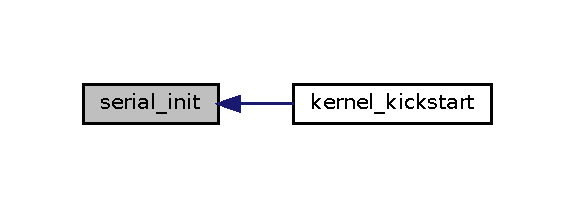
\includegraphics[width=276pt]{serial_8h_ac8063a6773891c77be25ad972f915f35_icgraph}
\end{center}
\end{figure}
\mbox{\Hypertarget{serial_8h_a28c404f87f73ce3d02c889d4792d6a19}\label{serial_8h_a28c404f87f73ce3d02c889d4792d6a19}} 
\index{serial.\+h@{serial.\+h}!serial\+\_\+write@{serial\+\_\+write}}
\index{serial\+\_\+write@{serial\+\_\+write}!serial.\+h@{serial.\+h}}
\subsubsection{\texorpdfstring{serial\+\_\+write()}{serial\_write()}}
{\footnotesize\ttfamily \hyperlink{error__types_8h_acf146bc98f60f47c79d782f7523e339c}{E\+R\+R\+O\+R\+\_\+\+C\+O\+D\+E\+\_\+E} serial\+\_\+write (\begin{DoxyParamCaption}\item[{const char $\ast$}]{str,  }\item[{const \hyperlink{stddef_8h_aa9d55e2f20e580b7445617d0d12fff6e}{size\+\_\+t}}]{length }\end{DoxyParamCaption})}



Writes a string of characters to the serial line. 

Writes a string of characters to the serial line. The line should have been initialized. If the serial line is not ready, this function has no effect.


\begin{DoxyParams}[1]{Parameters}
\mbox{\tt in}  & {\em str} & The string to send to the serial line. \\
\hline
\mbox{\tt in}  & {\em length} & The length of the string to send to the serial line.\\
\hline
\end{DoxyParams}
\begin{DoxyReturn}{Returns}
N\+O\+\_\+\+E\+R\+R\+OR is returned in case of success. Otherwise an error code is returned. Please refer to the list of the standard error codes. 
\end{DoxyReturn}


Definition at line 489 of file bsp\+\_\+usart.\+c.


\begin{DoxyCode}
490 \{
491     \textcolor{keywordtype}{size\_t} i;
492 
493     \textcolor{keywordflow}{if}(\hyperlink{bsp__usart_8c_ad317e99f056e9ce535815fcdd1697c93}{usart\_init\_state} == 0)
494     \{
495 \textcolor{preprocessor}{#if KERNEL\_LOG\_LEVEL == ERROR\_LOG\_LEVEL
}
496         \hyperlink{logger_8h_a580bb63c1418b2fc8456f9b6c5b6d39d}{KERNEL\_LOG\_ERROR}(\textcolor{stringliteral}{"Serial needs to be initialized"}, 
497                          \hyperlink{error__types_8h_a4db9ee29f2ff83c71567c12f6bfbf28ca10cd4fcc87eb6469778e1c547cf94877}{ERROR\_NEED\_INIT}, 
498                          \textcolor{keyword}{sizeof}(\hyperlink{error__types_8h_a4db9ee29f2ff83c71567c12f6bfbf28ca10cd4fcc87eb6469778e1c547cf94877}{ERROR\_NEED\_INIT}), 
499                          \hyperlink{error__types_8h_a4db9ee29f2ff83c71567c12f6bfbf28ca10cd4fcc87eb6469778e1c547cf94877}{ERROR\_NEED\_INIT});
500 \textcolor{preprocessor}{#endif        
}
501         \textcolor{keywordflow}{return} \hyperlink{error__types_8h_a4db9ee29f2ff83c71567c12f6bfbf28ca9af911a6ba1c32ce22213d689cb59f86}{ERROR\_ALREADY\_INIT};
502     \}
503 
504     \textcolor{keywordflow}{for}(i = 0; i < length; ++i)
505     \{
506         \textcolor{comment}{/* Wait for serial line to be ready to transmit */}
507         \textcolor{keywordflow}{while}((*\hyperlink{bsp__usart_8h_aa902cd686824df937532dbdb8a9c9dac}{USART2\_SR\_REGISTER} & \hyperlink{bsp__usart_8h_a65e9cddf0890113d405342f1d8b5b980}{USART\_SR\_TXE}) == 0);
508 
509         *\hyperlink{bsp__usart_8h_a8e09469004e7199b63ac9df19afd41a5}{USART2\_DR\_REGISTER} = *str++;
510     \}
511 
512     \textcolor{keywordflow}{return} \hyperlink{error__types_8h_a4db9ee29f2ff83c71567c12f6bfbf28cabf350750d0d4fabd8954c0f1e9bbae94}{NO\_ERROR};
513 \}
\end{DoxyCode}
Here is the call graph for this function\+:\nopagebreak
\begin{figure}[H]
\begin{center}
\leavevmode
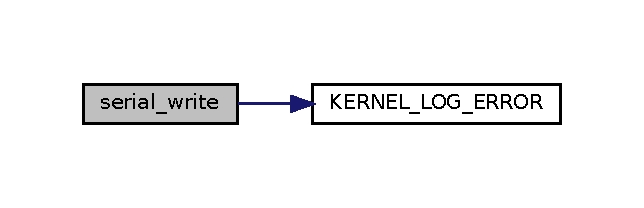
\includegraphics[width=309pt]{serial_8h_a28c404f87f73ce3d02c889d4792d6a19_cgraph}
\end{center}
\end{figure}
Here is the caller graph for this function\+:\nopagebreak
\begin{figure}[H]
\begin{center}
\leavevmode
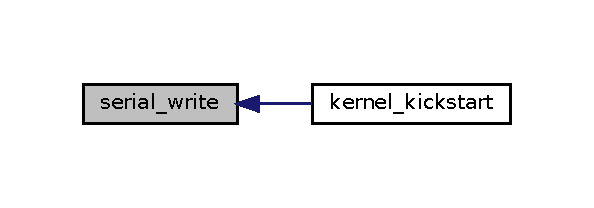
\includegraphics[width=285pt]{serial_8h_a28c404f87f73ce3d02c889d4792d6a19_icgraph}
\end{center}
\end{figure}

\hypertarget{bsp__clocks_8h}{}\section{Kernel/\+Sources/arch/board/stm32/f401re/includes/bsp\+\_\+clocks.h File Reference}
\label{bsp__clocks_8h}\index{Kernel/\+Sources/arch/board/stm32/f401re/includes/bsp\+\_\+clocks.\+h@{Kernel/\+Sources/arch/board/stm32/f401re/includes/bsp\+\_\+clocks.\+h}}
{\ttfamily \#include \char`\"{}error\+\_\+types.\+h\char`\"{}}\newline
{\ttfamily \#include \char`\"{}bsp\+\_\+usart.\+h\char`\"{}}\newline
{\ttfamily \#include \char`\"{}bsp\+\_\+gpio.\+h\char`\"{}}\newline
{\ttfamily \#include \char`\"{}stdint.\+h\char`\"{}}\newline
Include dependency graph for bsp\+\_\+clocks.\+h\+:\nopagebreak
\begin{figure}[H]
\begin{center}
\leavevmode
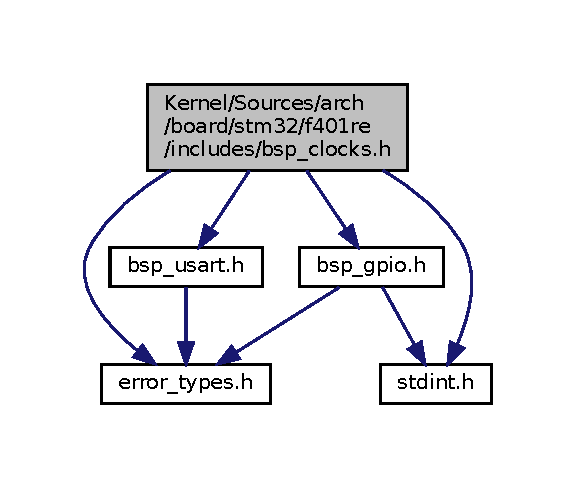
\includegraphics[width=276pt]{bsp__clocks_8h__incl}
\end{center}
\end{figure}
This graph shows which files directly or indirectly include this file\+:\nopagebreak
\begin{figure}[H]
\begin{center}
\leavevmode
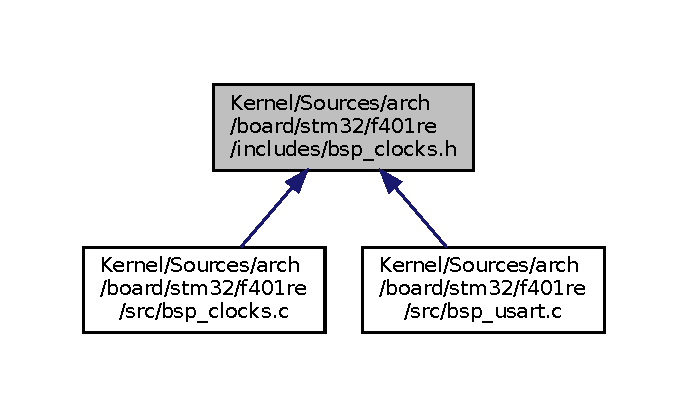
\includegraphics[width=330pt]{bsp__clocks_8h__dep__incl}
\end{center}
\end{figure}
\subsection*{Macros}
\begin{DoxyCompactItemize}
\item 
\#define \hyperlink{bsp__clocks_8h_a5d90893e6a5c6e0be4c7d78220a99e72}{R\+C\+C\+\_\+\+C\+R\+\_\+\+A\+D\+D\+R\+E\+SS}~0x40023800
\begin{DoxyCompactList}\small\item\em R\+CC Control Register address. \end{DoxyCompactList}\item 
\#define \hyperlink{bsp__clocks_8h_a2fcf7c04f16b1dd27c577a9a14c5ff96}{R\+C\+C\+\_\+\+C\+R\+\_\+\+R\+E\+G\+I\+S\+T\+ER}~((volatile \hyperlink{stdint_8h_a324c5d28c0d82f502a234ab99efac87a}{uint32\+\_\+t}$\ast$)\hyperlink{bsp__clocks_8h_a5d90893e6a5c6e0be4c7d78220a99e72}{R\+C\+C\+\_\+\+C\+R\+\_\+\+A\+D\+D\+R\+E\+SS})
\item 
\#define \hyperlink{bsp__clocks_8h_aefbe0661a046e5156a8d1efb28acc7c1}{R\+C\+C\+\_\+\+P\+L\+L\+C\+F\+G\+R\+\_\+\+A\+D\+D\+R\+E\+SS}~0x40023804
\begin{DoxyCompactList}\small\item\em R\+CC P\+LL Configuration Register address. \end{DoxyCompactList}\item 
\#define \hyperlink{bsp__clocks_8h_ad2d60b66a5292f1c04c7c3ebfe9df335}{R\+C\+C\+\_\+\+P\+L\+L\+C\+F\+G\+R\+\_\+\+R\+E\+G\+I\+S\+T\+ER}~((volatile \hyperlink{stdint_8h_a324c5d28c0d82f502a234ab99efac87a}{uint32\+\_\+t}$\ast$)\hyperlink{bsp__clocks_8h_aefbe0661a046e5156a8d1efb28acc7c1}{R\+C\+C\+\_\+\+P\+L\+L\+C\+F\+G\+R\+\_\+\+A\+D\+D\+R\+E\+SS})
\item 
\#define \hyperlink{bsp__clocks_8h_a91cfae801ddf98df5893db0b9a9027dd}{R\+C\+C\+\_\+\+C\+F\+G\+R\+\_\+\+A\+D\+D\+R\+E\+SS}~0x40023808
\begin{DoxyCompactList}\small\item\em R\+CC Configuration Register address. \end{DoxyCompactList}\item 
\#define \hyperlink{bsp__clocks_8h_ac454715dd9c4f8ba957cc53f318c58ac}{R\+C\+C\+\_\+\+C\+F\+G\+R\+\_\+\+R\+E\+G\+I\+S\+T\+ER}~((volatile \hyperlink{stdint_8h_a324c5d28c0d82f502a234ab99efac87a}{uint32\+\_\+t}$\ast$)\hyperlink{bsp__clocks_8h_a91cfae801ddf98df5893db0b9a9027dd}{R\+C\+C\+\_\+\+C\+F\+G\+R\+\_\+\+A\+D\+D\+R\+E\+SS})
\item 
\#define \hyperlink{bsp__clocks_8h_aeeed0a38fad05745c2280f5ae24af5c7}{R\+C\+C\+\_\+\+A\+H\+B1\+E\+N\+R\+\_\+\+A\+D\+D\+R\+E\+SS}~0x40023830
\begin{DoxyCompactList}\small\item\em R\+CC A\+H\+B1 peripheral clock enable register address. \end{DoxyCompactList}\item 
\#define \hyperlink{bsp__clocks_8h_a4c6aae1c96c5acee8a320c6b2a8aaee5}{R\+C\+C\+\_\+\+A\+H\+B1\+E\+N\+R\+\_\+\+R\+E\+G\+I\+S\+T\+ER}~((volatile \hyperlink{stdint_8h_a324c5d28c0d82f502a234ab99efac87a}{uint32\+\_\+t}$\ast$)\hyperlink{bsp__clocks_8h_aeeed0a38fad05745c2280f5ae24af5c7}{R\+C\+C\+\_\+\+A\+H\+B1\+E\+N\+R\+\_\+\+A\+D\+D\+R\+E\+SS})
\item 
\#define \hyperlink{bsp__clocks_8h_aceec3e2cc1ffd17a8637d7437e1401fa}{R\+C\+C\+\_\+\+A\+P\+B1\+E\+N\+R\+\_\+\+A\+D\+D\+R\+E\+SS}~0x40023840
\begin{DoxyCompactList}\small\item\em R\+CC A\+P\+B1 peripheral clock enable register address. \end{DoxyCompactList}\item 
\#define \hyperlink{bsp__clocks_8h_aae3fa9b2133a67e3ca65db35f8ac9a4c}{R\+C\+C\+\_\+\+A\+P\+B1\+E\+N\+R\+\_\+\+R\+E\+G\+I\+S\+T\+ER}~((volatile \hyperlink{stdint_8h_a324c5d28c0d82f502a234ab99efac87a}{uint32\+\_\+t}$\ast$)\hyperlink{bsp__clocks_8h_aceec3e2cc1ffd17a8637d7437e1401fa}{R\+C\+C\+\_\+\+A\+P\+B1\+E\+N\+R\+\_\+\+A\+D\+D\+R\+E\+SS})
\item 
\#define \hyperlink{bsp__clocks_8h_a5dfd160b628ef272a6f6cf6b0476afab}{R\+C\+C\+\_\+\+A\+P\+B2\+E\+N\+R\+\_\+\+A\+D\+D\+R\+E\+SS}~0x40023844
\begin{DoxyCompactList}\small\item\em R\+CC A\+P\+B2 peripheral clock enable register address. \end{DoxyCompactList}\item 
\#define \hyperlink{bsp__clocks_8h_aae721f66e88c2e4264580d95d5ffdd59}{R\+C\+C\+\_\+\+A\+P\+B2\+E\+N\+R\+\_\+\+R\+E\+G\+I\+S\+T\+ER}~((volatile \hyperlink{stdint_8h_a324c5d28c0d82f502a234ab99efac87a}{uint32\+\_\+t}$\ast$)\hyperlink{bsp__clocks_8h_a5dfd160b628ef272a6f6cf6b0476afab}{R\+C\+C\+\_\+\+A\+P\+B2\+E\+N\+R\+\_\+\+A\+D\+D\+R\+E\+SS})
\item 
\#define \hyperlink{bsp__clocks_8h_a7a9d56a8aa1fa0f519ecbdf0d19dd4da}{R\+C\+C\+\_\+\+A\+P\+B2\+E\+N\+R\+\_\+\+S\+Y\+S\+C\+F\+G\+EN}~0x00004000
\begin{DoxyCompactList}\small\item\em A\+P\+B2\+E\+NR System configuration controller clock enable. \end{DoxyCompactList}\item 
\#define \hyperlink{bsp__clocks_8h_a6ff46fb3b30fc6792e4fd18fcb0941b5}{R\+C\+C\+\_\+\+A\+H\+B1\+E\+N\+R\+\_\+\+G\+P\+I\+O\+A\+EN}~0x00000001
\begin{DoxyCompactList}\small\item\em A\+H\+B1\+E\+NR G\+P\+IO A enable. \end{DoxyCompactList}\item 
\#define \hyperlink{bsp__clocks_8h_ad7f408f92e7fd49b0957b8cb4ff31ca5}{R\+C\+C\+\_\+\+A\+H\+B1\+E\+N\+R\+\_\+\+G\+P\+I\+O\+B\+EN}~0x00000002
\begin{DoxyCompactList}\small\item\em A\+H\+B1\+E\+NR G\+P\+IO B enable. \end{DoxyCompactList}\item 
\#define \hyperlink{bsp__clocks_8h_ae8a8b42e33aef2a7bc2d41ad9d231733}{R\+C\+C\+\_\+\+A\+H\+B1\+E\+N\+R\+\_\+\+G\+P\+I\+O\+C\+EN}~0x00000004
\begin{DoxyCompactList}\small\item\em A\+H\+B1\+E\+NR G\+P\+IO C enable. \end{DoxyCompactList}\item 
\#define \hyperlink{bsp__clocks_8h_aebd8146e91c76f14af8dfe78a1c2d916}{R\+C\+C\+\_\+\+A\+H\+B1\+E\+N\+R\+\_\+\+G\+P\+I\+O\+D\+EN}~0x00000008
\begin{DoxyCompactList}\small\item\em A\+H\+B1\+E\+NR G\+P\+IO D enable. \end{DoxyCompactList}\item 
\#define \hyperlink{bsp__clocks_8h_a67a9094e0e464eaa8e25f854f90abfc6}{R\+C\+C\+\_\+\+A\+H\+B1\+E\+N\+R\+\_\+\+G\+P\+I\+O\+E\+EN}~0x00000010
\begin{DoxyCompactList}\small\item\em A\+H\+B1\+E\+NR G\+P\+IO E enable. \end{DoxyCompactList}\item 
\#define \hyperlink{bsp__clocks_8h_adb16afc550121895822ebb22108196b6}{R\+C\+C\+\_\+\+A\+H\+B1\+E\+N\+R\+\_\+\+G\+P\+I\+O\+H\+EN}~0x00000080
\begin{DoxyCompactList}\small\item\em A\+H\+B1\+E\+NR G\+P\+IO H enable. \end{DoxyCompactList}\item 
\#define \hyperlink{bsp__clocks_8h_a5c19997ccd28464b80a7c3325da0ca60}{R\+C\+C\+\_\+\+A\+P\+B1\+E\+N\+R\+\_\+\+P\+W\+R\+EN}~0x10000000
\begin{DoxyCompactList}\small\item\em A\+P\+B1\+E\+NR Power interface clock enable. \end{DoxyCompactList}\item 
\#define \hyperlink{bsp__clocks_8h_ab840af4f735ec36419d61c7db3cfa00d}{R\+C\+C\+\_\+\+A\+P\+B1\+E\+N\+R\+\_\+\+U\+S\+A\+R\+T2\+EN}~0x00020000
\begin{DoxyCompactList}\small\item\em A\+P\+B1\+E\+NR U\+S\+A\+R\+T2 clock enable. \end{DoxyCompactList}\item 
\#define \hyperlink{bsp__clocks_8h_a4666bb90842e8134b32e6a34a0f165f3}{R\+C\+C\+\_\+\+A\+P\+B2\+E\+N\+R\+\_\+\+U\+S\+A\+R\+T1\+EN}~0x00000010
\begin{DoxyCompactList}\small\item\em A\+P\+B2\+E\+NR U\+S\+A\+R\+T1 clock enable. \end{DoxyCompactList}\item 
\#define \hyperlink{bsp__clocks_8h_a0569d91f3b18ae130b7a09e0100c4459}{R\+C\+C\+\_\+\+A\+P\+B2\+E\+N\+R\+\_\+\+U\+S\+A\+R\+T6\+EN}~0x00000020
\begin{DoxyCompactList}\small\item\em A\+P\+B2\+E\+NR U\+S\+A\+R\+T6 clock enable. \end{DoxyCompactList}\item 
\#define \hyperlink{bsp__clocks_8h_a7354703f289244a71753debf3ae26e46}{R\+C\+C\+\_\+\+C\+R\+\_\+\+P\+L\+L\+I2\+S\+R\+DY}~0x08000000
\begin{DoxyCompactList}\small\item\em R\+C\+C\+\_\+\+CR P\+L\+L\+I2S ready flag. \end{DoxyCompactList}\item 
\#define \hyperlink{bsp__clocks_8h_a3ccb8964b640530f1080f9ea549d8133}{R\+C\+C\+\_\+\+C\+R\+\_\+\+P\+L\+L\+I2\+S\+ON}~0x04000000
\begin{DoxyCompactList}\small\item\em R\+C\+C\+\_\+\+CR P\+L\+L\+I2S enabled. \end{DoxyCompactList}\item 
\#define \hyperlink{bsp__clocks_8h_afa12d7ac6a7f0f91d066aeb2c6071888}{R\+C\+C\+\_\+\+C\+R\+\_\+\+P\+L\+L\+R\+DY}~0x02000000
\begin{DoxyCompactList}\small\item\em R\+C\+C\+\_\+\+CR P\+LL ready flag. \end{DoxyCompactList}\item 
\#define \hyperlink{bsp__clocks_8h_ad0e73d5b0a4883e074d40029b49ee47e}{R\+C\+C\+\_\+\+C\+R\+\_\+\+P\+L\+L\+ON}~0x01000000
\begin{DoxyCompactList}\small\item\em R\+C\+C\+\_\+\+CR P\+LL enabled. \end{DoxyCompactList}\item 
\#define \hyperlink{bsp__clocks_8h_a12241a92893b4023a40e85d3b371ac05}{R\+C\+C\+\_\+\+C\+R\+\_\+\+H\+S\+I\+T\+R\+I\+M\+\_\+\+D\+EF}~0x00000080
\begin{DoxyCompactList}\small\item\em R\+C\+C\+\_\+\+CR H\+SI clock default trimming value. \end{DoxyCompactList}\item 
\#define \hyperlink{bsp__clocks_8h_af4fcacf94a97f7d49a70e089b39cf474}{R\+C\+C\+\_\+\+C\+R\+\_\+\+H\+S\+I\+ON}~0x00000001
\begin{DoxyCompactList}\small\item\em R\+C\+C\+\_\+\+CR H\+SI clock enabled. \end{DoxyCompactList}\item 
\#define \hyperlink{bsp__clocks_8h_a9dbac3f2bc04f04ebafe1e66ae3fcf0d}{R\+C\+C\+\_\+\+C\+R\+\_\+\+H\+S\+I\+R\+DY}~0x00000002
\begin{DoxyCompactList}\small\item\em R\+C\+C\+\_\+\+CR H\+SI clock ready flag. \end{DoxyCompactList}\item 
\#define \hyperlink{bsp__clocks_8h_acbac8bae4f0808b3c3a5185aa10081fb}{R\+C\+C\+\_\+\+C\+F\+G\+R\+\_\+\+S\+W\+\_\+\+H\+SI}~0x00000000
\begin{DoxyCompactList}\small\item\em R\+C\+C\+\_\+\+C\+F\+GR System clock switch to H\+SI value. \end{DoxyCompactList}\item 
\#define \hyperlink{bsp__clocks_8h_afb563f217242d969f4355d0818fde705}{R\+C\+C\+\_\+\+C\+F\+G\+R\+\_\+\+S\+W\+\_\+\+H\+SE}~0x00000001
\begin{DoxyCompactList}\small\item\em R\+C\+C\+\_\+\+C\+F\+GR System clock switch to H\+SE value. \end{DoxyCompactList}\item 
\#define \hyperlink{bsp__clocks_8h_a87389cacb2eaf53730da13a2a33cd487}{R\+C\+C\+\_\+\+C\+F\+G\+R\+\_\+\+S\+W\+\_\+\+P\+LL}~0x00000002
\begin{DoxyCompactList}\small\item\em R\+C\+C\+\_\+\+C\+F\+GR System clock switch to P\+LL value. \end{DoxyCompactList}\item 
\#define \hyperlink{bsp__clocks_8h_a6764639cf221e1ebc0b5448dcaed590a}{R\+C\+C\+\_\+\+C\+F\+G\+R\+\_\+\+S\+W\+S\+\_\+\+H\+SI}~0x00000000
\begin{DoxyCompactList}\small\item\em R\+C\+C\+\_\+\+C\+F\+GR System clock switch to H\+SI status value. \end{DoxyCompactList}\item 
\#define \hyperlink{bsp__clocks_8h_ae09a0202f441c1a43e69c62331d50a08}{R\+C\+C\+\_\+\+C\+F\+G\+R\+\_\+\+S\+W\+S\+\_\+\+H\+SE}~0x00000004
\begin{DoxyCompactList}\small\item\em R\+C\+C\+\_\+\+C\+F\+GR System clock switch to H\+SE status value. \end{DoxyCompactList}\item 
\#define \hyperlink{bsp__clocks_8h_a2c67e2279804a83ef24438267d9d4a6c}{R\+C\+C\+\_\+\+C\+F\+G\+R\+\_\+\+S\+W\+S\+\_\+\+P\+LL}~0x00000008
\begin{DoxyCompactList}\small\item\em R\+C\+C\+\_\+\+C\+F\+GR System clock switch to P\+LL status value. \end{DoxyCompactList}\item 
\#define \hyperlink{bsp__clocks_8h_a1351ccf5f6a5d9a6b91c4f533688d8fb}{R\+C\+C\+\_\+\+C\+F\+G\+R\+\_\+\+H\+P\+R\+E\+\_\+\+EN}~0x00000080
\begin{DoxyCompactList}\small\item\em R\+C\+C\+\_\+\+C\+F\+GR A\+HB prescaller enabled state. \end{DoxyCompactList}\item 
\#define \hyperlink{bsp__clocks_8h_a3fe59bf63a37a12304f37d7babec3eeb}{R\+C\+C\+\_\+\+C\+F\+G\+R\+\_\+\+H\+R\+P\+E\+\_\+\+D\+I\+V1}~0x00000000
\begin{DoxyCompactList}\small\item\em R\+C\+C\+\_\+\+C\+F\+GR A\+HB prescaller value. \end{DoxyCompactList}\item 
\#define \hyperlink{bsp__clocks_8h_a7a4503de78658d3271cb5494adc96e41}{R\+C\+C\+\_\+\+C\+F\+G\+R\+\_\+\+P\+P\+R\+E1\+\_\+\+EN}~0x00001000
\begin{DoxyCompactList}\small\item\em R\+C\+C\+\_\+\+C\+F\+GR A\+PB LS prescaller enabled state. \end{DoxyCompactList}\item 
\#define \hyperlink{bsp__clocks_8h_af832ad6844c907d9bb37c1536defcb0d}{R\+C\+C\+\_\+\+C\+F\+G\+R\+\_\+\+P\+P\+R\+E1\+\_\+\+D\+I\+V2}~0x00001000
\begin{DoxyCompactList}\small\item\em R\+C\+C\+\_\+\+C\+F\+GR A\+PB LS prescaller value. \end{DoxyCompactList}\item 
\#define \hyperlink{bsp__clocks_8h_a1a384b58d9f246cb60ed0d0bfa92cbf4}{R\+C\+C\+\_\+\+C\+F\+G\+R\+\_\+\+P\+P\+R\+E2\+\_\+\+EN}~0x00008000
\begin{DoxyCompactList}\small\item\em R\+C\+C\+\_\+\+C\+F\+GR A\+PB HS prescaller enabled state. \end{DoxyCompactList}\item 
\#define \hyperlink{bsp__clocks_8h_a247aebf1999a38ea07785558d277bb1a}{R\+C\+C\+\_\+\+C\+F\+G\+R\+\_\+\+P\+P\+R\+E2\+\_\+\+D\+I\+V1}~0x00000000
\begin{DoxyCompactList}\small\item\em R\+C\+C\+\_\+\+C\+F\+GR A\+PB HS prescaller value. \end{DoxyCompactList}\item 
\#define \hyperlink{bsp__clocks_8h_afaac3bc429eaa475ca5e431a020d4c67}{R\+C\+C\+\_\+\+P\+L\+L\+C\+F\+G\+R\+\_\+\+P\+L\+L\+M\+\_\+\+M\+A\+SK}~0x0000003F
\begin{DoxyCompactList}\small\item\em R\+C\+C\+\_\+\+P\+L\+L\+C\+F\+GR P\+L\+LM bit mask. \end{DoxyCompactList}\item 
\#define \hyperlink{bsp__clocks_8h_a90997335764397eb4be02c23676cda4a}{R\+C\+C\+\_\+\+P\+L\+L\+C\+F\+G\+R\+\_\+\+P\+L\+L\+N\+\_\+\+M\+A\+SK}~0x00007\+F\+C0
\begin{DoxyCompactList}\small\item\em R\+C\+C\+\_\+\+P\+L\+L\+C\+F\+GR P\+L\+LN bit mask. \end{DoxyCompactList}\item 
\#define \hyperlink{bsp__clocks_8h_a40a7c5938dfdd0ab63dcf3b203da7dd4}{R\+C\+C\+\_\+\+P\+L\+L\+C\+F\+G\+R\+\_\+\+P\+L\+L\+P\+\_\+\+M\+A\+SK}~0x00030000
\begin{DoxyCompactList}\small\item\em R\+C\+C\+\_\+\+P\+L\+L\+C\+F\+GR P\+L\+LP bit mask. \end{DoxyCompactList}\item 
\#define \hyperlink{bsp__clocks_8h_a6c5c6a2e8d760ad7da85ae2c8076ee31}{R\+C\+C\+\_\+\+P\+L\+L\+C\+F\+G\+R\+\_\+\+P\+L\+L\+S\+R\+C\+\_\+\+M\+A\+SK}~0x00400000
\begin{DoxyCompactList}\small\item\em R\+C\+C\+\_\+\+P\+L\+L\+C\+F\+GR P\+L\+L\+S\+RC bit mask. \end{DoxyCompactList}\item 
\#define \hyperlink{bsp__clocks_8h_ad4784939ce13e81f2cc64dda2b5d8770}{R\+C\+C\+\_\+\+P\+L\+L\+C\+F\+G\+R\+\_\+\+P\+L\+L\+Q\+\_\+\+M\+A\+SK}~0x0\+F000000
\begin{DoxyCompactList}\small\item\em R\+C\+C\+\_\+\+P\+L\+L\+C\+F\+GR P\+L\+LQ bit mask. \end{DoxyCompactList}\item 
\#define \hyperlink{bsp__clocks_8h_a7e5e28699fe923870e15fef3651ff3ef}{R\+C\+C\+\_\+\+C\+F\+G\+R\+\_\+\+S\+W\+\_\+\+M\+A\+SK}~0x00000003
\begin{DoxyCompactList}\small\item\em R\+C\+C\+\_\+\+C\+F\+GR SW bit mask. \end{DoxyCompactList}\item 
\#define \hyperlink{bsp__clocks_8h_a451045d952eb1caaa0090c9e8dc75082}{R\+C\+C\+\_\+\+C\+F\+G\+R\+\_\+\+S\+W\+S\+\_\+\+M\+A\+SK}~0x0000000C
\begin{DoxyCompactList}\small\item\em R\+C\+C\+\_\+\+C\+F\+GR S\+WS bit mask. \end{DoxyCompactList}\item 
\#define \hyperlink{bsp__clocks_8h_a7b024c33f9bd185d923b55af2360fec5}{R\+C\+C\+\_\+\+C\+F\+G\+R\+\_\+\+H\+R\+P\+E\+\_\+\+M\+A\+SK}~0x000000\+F0
\begin{DoxyCompactList}\small\item\em R\+C\+C\+\_\+\+C\+F\+GR H\+R\+PE bit mask. \end{DoxyCompactList}\item 
\#define \hyperlink{bsp__clocks_8h_a2ff38fa14905e578752b706e5c29b146}{R\+C\+C\+\_\+\+C\+F\+G\+R\+\_\+\+H\+P\+R\+E\+\_\+\+V\+A\+L\+\_\+\+M\+A\+SK}~0x00000070
\begin{DoxyCompactList}\small\item\em R\+C\+C\+\_\+\+C\+F\+GR H\+R\+PE value bit mask. \end{DoxyCompactList}\item 
\#define \hyperlink{bsp__clocks_8h_a1220a63e00de9ff4a2a45474ead3662d}{R\+C\+C\+\_\+\+C\+F\+G\+R\+\_\+\+P\+P\+R\+E1\+\_\+\+M\+A\+SK}~0x00001\+C00
\begin{DoxyCompactList}\small\item\em R\+C\+C\+\_\+\+C\+F\+GR P\+P\+R\+E1 bit mask. \end{DoxyCompactList}\item 
\#define \hyperlink{bsp__clocks_8h_aebda6f102f65bc354b95232527021aba}{R\+C\+C\+\_\+\+C\+F\+G\+R\+\_\+\+P\+P\+R\+E1\+\_\+\+V\+A\+L\+\_\+\+M\+A\+SK}~0x00000\+C00
\begin{DoxyCompactList}\small\item\em R\+C\+C\+\_\+\+C\+F\+GR P\+P\+R\+E1 value bit mask. \end{DoxyCompactList}\item 
\#define \hyperlink{bsp__clocks_8h_a41aef118b0611444caa87df8ea302dc2}{R\+C\+C\+\_\+\+C\+F\+G\+R\+\_\+\+P\+P\+R\+E2\+\_\+\+M\+A\+SK}~0x0000\+E000
\begin{DoxyCompactList}\small\item\em R\+C\+C\+\_\+\+C\+F\+GR P\+P\+R\+E2 bit mask. \end{DoxyCompactList}\item 
\#define \hyperlink{bsp__clocks_8h_adb27fe14c6c6c2cb20f13aaf86f0900a}{R\+C\+C\+\_\+\+C\+F\+G\+R\+\_\+\+P\+P\+R\+E2\+\_\+\+V\+A\+L\+\_\+\+M\+A\+SK}~0x00006000
\begin{DoxyCompactList}\small\item\em R\+C\+C\+\_\+\+C\+F\+GR P\+P\+R\+E2 value bit mask. \end{DoxyCompactList}\item 
\#define \hyperlink{bsp__clocks_8h_a73f9913edb8b30eb2b8aa1b5d29b297e}{R\+C\+C\+\_\+\+C\+R\+\_\+\+H\+S\+I\+T\+R\+I\+M\+\_\+\+M\+A\+SK}~0x000000\+F8
\begin{DoxyCompactList}\small\item\em H\+SI clock trimming field mask. \end{DoxyCompactList}\item 
\#define \hyperlink{bsp__clocks_8h_add5fc49687031bdd44fca9c909f74fe0}{R\+C\+C\+\_\+\+P\+L\+L\+C\+F\+G\+R\+\_\+\+P\+L\+L\+M\+\_\+\+O\+F\+F\+S\+ET}~0
\begin{DoxyCompactList}\small\item\em R\+C\+C\+\_\+\+P\+L\+L\+C\+F\+GR P\+L\+LM bit field offset. \end{DoxyCompactList}\item 
\#define \hyperlink{bsp__clocks_8h_adc0f70732fb3d933c96d741f27baec35}{R\+C\+C\+\_\+\+P\+L\+L\+C\+F\+G\+R\+\_\+\+P\+L\+L\+N\+\_\+\+O\+F\+F\+S\+ET}~6
\begin{DoxyCompactList}\small\item\em R\+C\+C\+\_\+\+P\+L\+L\+C\+F\+GR P\+L\+LN bit field offset. \end{DoxyCompactList}\item 
\#define \hyperlink{bsp__clocks_8h_a9a6c6234e6c59e7638d1a8edd237f591}{R\+C\+C\+\_\+\+P\+L\+L\+C\+F\+G\+R\+\_\+\+P\+L\+L\+P\+\_\+\+O\+F\+F\+S\+ET}~16
\begin{DoxyCompactList}\small\item\em R\+C\+C\+\_\+\+P\+L\+L\+C\+F\+GR P\+L\+LP bit field offset. \end{DoxyCompactList}\item 
\#define \hyperlink{bsp__clocks_8h_a001728588571f89b2b52e6a903e66395}{R\+C\+C\+\_\+\+P\+L\+L\+C\+F\+G\+R\+\_\+\+P\+L\+L\+S\+R\+C\+\_\+\+O\+F\+F\+S\+ET}~22
\begin{DoxyCompactList}\small\item\em R\+C\+C\+\_\+\+P\+L\+L\+C\+F\+GR P\+L\+L\+S\+RC bit field offset. \end{DoxyCompactList}\item 
\#define \hyperlink{bsp__clocks_8h_aa47b1576488cea5e741f58cce74337c9}{R\+C\+C\+\_\+\+P\+L\+L\+C\+F\+G\+R\+\_\+\+P\+L\+L\+Q\+\_\+\+O\+F\+F\+S\+ET}~24
\begin{DoxyCompactList}\small\item\em R\+C\+C\+\_\+\+P\+L\+L\+C\+F\+GR P\+L\+LQ bit field offset. \end{DoxyCompactList}\item 
\#define \hyperlink{bsp__clocks_8h_adca5b474c16bb5c9b4bbedfabeba8e25}{R\+C\+C\+\_\+\+C\+F\+G\+R\+\_\+\+H\+R\+P\+E\+\_\+\+O\+F\+F\+S\+ET}~4
\begin{DoxyCompactList}\small\item\em R\+C\+C\+\_\+\+C\+F\+GR H\+P\+RE bit field offset. \end{DoxyCompactList}\item 
\#define \hyperlink{bsp__clocks_8h_a1f605f808c9ab7530142dd8808e83a22}{R\+C\+C\+\_\+\+C\+F\+G\+R\+\_\+\+P\+P\+R\+E1\+\_\+\+O\+F\+F\+S\+ET}~10
\begin{DoxyCompactList}\small\item\em R\+C\+C\+\_\+\+C\+F\+GR P\+P\+R\+E1 bit field offset. \end{DoxyCompactList}\item 
\#define \hyperlink{bsp__clocks_8h_a906e390883db586903c4b1144a182e47}{R\+C\+C\+\_\+\+C\+F\+G\+R\+\_\+\+P\+P\+R\+E2\+\_\+\+O\+F\+F\+S\+ET}~13
\begin{DoxyCompactList}\small\item\em R\+C\+C\+\_\+\+C\+F\+GR P\+P\+R\+E2 bit field offset. \end{DoxyCompactList}\item 
\#define \hyperlink{bsp__clocks_8h_adc4eb2ce50286dc96d4976b9689be1d7}{R\+C\+C\+\_\+\+P\+L\+L\+M\+\_\+\+V\+A\+L\+UE}~16
\begin{DoxyCompactList}\small\item\em Division factor for input clock. Divide by 16 the H\+SI clock. \end{DoxyCompactList}\item 
\#define \hyperlink{bsp__clocks_8h_a11fa93ae89931a632e06eb0694ff62b7}{R\+C\+C\+\_\+\+P\+L\+L\+N\+\_\+\+V\+A\+L\+UE}~336
\begin{DoxyCompactList}\small\item\em Multiply factor for system clock. Multiply by 336 the V\+CO clock. \end{DoxyCompactList}\item 
\#define \hyperlink{bsp__clocks_8h_a9ad812030f6e208e79df8e9bddb96c19}{R\+C\+C\+\_\+\+P\+L\+L\+P\+\_\+\+V\+A\+L\+UE}~1
\begin{DoxyCompactList}\small\item\em Division factor for system clock. Divide by 4 the V\+CO clock. \end{DoxyCompactList}\item 
\#define \hyperlink{bsp__clocks_8h_a0babc931753727d1ee6b56d41a51f598}{R\+C\+C\+\_\+\+P\+L\+L\+Q\+\_\+\+V\+A\+L\+UE}~8
\begin{DoxyCompactList}\small\item\em Division factor for U\+SB O\+TG FS clock. Divide by 8 the V\+CO clock. \end{DoxyCompactList}\item 
\#define \hyperlink{bsp__clocks_8h_ae90c3d400891ac3355363979581bd924}{R\+C\+C\+\_\+\+P\+L\+L\+S\+R\+C\+\_\+\+V\+A\+L\+UE}~0
\begin{DoxyCompactList}\small\item\em P\+LL source clock set as H\+SI. \end{DoxyCompactList}\item 
\#define \hyperlink{bsp__clocks_8h_ae89e6b2d1e86b7fb4831cb013ece2c52}{R\+C\+C\+\_\+\+H\+S\+I\+\_\+\+B\+A\+S\+E\+\_\+\+F\+R\+EQ}~16000000
\begin{DoxyCompactList}\small\item\em H\+SI clock frequency. \end{DoxyCompactList}\item 
\#define \hyperlink{bsp__clocks_8h_a19d723f47200a1da259e9c147f2de258}{R\+C\+C\+\_\+\+H\+S\+E\+\_\+\+B\+A\+S\+E\+\_\+\+F\+R\+EQ}~0
\begin{DoxyCompactList}\small\item\em H\+SE clock frequency (does not exists on S\+T\+M\+F401\+RE) \end{DoxyCompactList}\end{DoxyCompactItemize}
\subsection*{Typedefs}
\begin{DoxyCompactItemize}
\item 
typedef enum \hyperlink{bsp__clocks_8h_ad0e92b49c1a7205e3460ca1e54fa9d70}{C\+L\+O\+C\+K\+\_\+\+I\+D\+E\+N\+T\+I\+F\+I\+ER} \hyperlink{bsp__clocks_8h_ac9d4d589a659370f313ef156f6eff0e8}{C\+L\+O\+C\+K\+\_\+\+I\+D\+E\+N\+T\+I\+F\+I\+E\+R\+\_\+T}
\begin{DoxyCompactList}\small\item\em Short hand for enum C\+L\+O\+C\+K\+\_\+\+I\+D\+E\+N\+T\+I\+F\+I\+ER. \end{DoxyCompactList}\end{DoxyCompactItemize}
\subsection*{Enumerations}
\begin{DoxyCompactItemize}
\item 
enum \hyperlink{bsp__clocks_8h_ad0e92b49c1a7205e3460ca1e54fa9d70}{C\+L\+O\+C\+K\+\_\+\+I\+D\+E\+N\+T\+I\+F\+I\+ER} \{ \newline
\hyperlink{bsp__clocks_8h_ad0e92b49c1a7205e3460ca1e54fa9d70a44aa8d3c1c8f980b372190786a4853f9}{B\+S\+P\+\_\+\+C\+L\+O\+C\+K\+\_\+\+I\+D\+\_\+\+S\+Y\+S\+C\+LK}, 
\hyperlink{bsp__clocks_8h_ad0e92b49c1a7205e3460ca1e54fa9d70a58357d0569548d6c2ba44f27e0aa6ba6}{B\+S\+P\+\_\+\+C\+L\+O\+C\+K\+\_\+\+I\+D\+\_\+\+H\+C\+LK}, 
\hyperlink{bsp__clocks_8h_ad0e92b49c1a7205e3460ca1e54fa9d70a265c9dec4478eb66904a2dbc6954e598}{B\+S\+P\+\_\+\+C\+L\+O\+C\+K\+\_\+\+I\+D\+\_\+\+F\+C\+LK}, 
\hyperlink{bsp__clocks_8h_ad0e92b49c1a7205e3460ca1e54fa9d70a0493d0bbd7edf1aebadb342c5c38f709}{B\+S\+P\+\_\+\+C\+L\+O\+C\+K\+\_\+\+I\+D\+\_\+\+P\+C\+L\+K1}, 
\newline
\hyperlink{bsp__clocks_8h_ad0e92b49c1a7205e3460ca1e54fa9d70aad62d8c78d2b4617724a82ec190a33ee}{B\+S\+P\+\_\+\+C\+L\+O\+C\+K\+\_\+\+I\+D\+\_\+\+P\+C\+L\+K2}, 
\hyperlink{bsp__clocks_8h_ad0e92b49c1a7205e3460ca1e54fa9d70aad46d3b8852f9a4d711c15164bf1c0d3}{B\+S\+P\+\_\+\+C\+L\+O\+C\+K\+\_\+\+I\+D\+\_\+\+A\+P\+B1\+\_\+\+T\+I\+M\+ER}, 
\hyperlink{bsp__clocks_8h_ad0e92b49c1a7205e3460ca1e54fa9d70a30cca3be6a7bad72d2c02e9b58ff4d50}{B\+S\+P\+\_\+\+C\+L\+O\+C\+K\+\_\+\+I\+D\+\_\+\+A\+P\+B2\+\_\+\+T\+I\+M\+ER}
 \}\begin{DoxyCompactList}\small\item\em Clock identifer enumeration. Stores all accessible B\+SP clocks. \end{DoxyCompactList}
\end{DoxyCompactItemize}
\subsection*{Functions}
\begin{DoxyCompactItemize}
\item 
\hyperlink{error__types_8h_acf146bc98f60f47c79d782f7523e339c}{E\+R\+R\+O\+R\+\_\+\+C\+O\+D\+E\+\_\+E} \hyperlink{bsp__clocks_8h_aaf01af602e17579af5e6af009ae7a557}{bsp\+\_\+clk\+\_\+usart\+\_\+enable} (const \hyperlink{bsp__usart_8h_a594f9d90a9a3875660da4512fb208cf9}{U\+S\+A\+R\+T\+\_\+\+I\+D\+E\+N\+T\+I\+F\+I\+E\+R\+\_\+E} usart\+\_\+id)
\begin{DoxyCompactList}\small\item\em Enables the U\+S\+A\+RT clocks. \end{DoxyCompactList}\item 
\hyperlink{error__types_8h_acf146bc98f60f47c79d782f7523e339c}{E\+R\+R\+O\+R\+\_\+\+C\+O\+D\+E\+\_\+E} \hyperlink{bsp__clocks_8h_a500b2e77b70c93b3f2b4a94cc9bcf79d}{bsp\+\_\+clk\+\_\+gpio\+\_\+enable} (const \hyperlink{bsp__gpio_8h_ab086506332275a2a873dfce02ed5a3b8}{G\+P\+I\+O\+\_\+\+I\+D\+E\+N\+T\+I\+F\+I\+E\+R\+\_\+E} gpio\+\_\+id)
\begin{DoxyCompactList}\small\item\em Enables the G\+P\+IO clocks. \end{DoxyCompactList}\item 
\hyperlink{error__types_8h_acf146bc98f60f47c79d782f7523e339c}{E\+R\+R\+O\+R\+\_\+\+C\+O\+D\+E\+\_\+E} \hyperlink{bsp__clocks_8h_a286d003315af35aa9dd72b86ba6d8420}{bsp\+\_\+clk\+\_\+sys\+\_\+init} (void)
\begin{DoxyCompactList}\small\item\em Initializes system clocks. \end{DoxyCompactList}\item 
\hyperlink{stdint_8h_a324c5d28c0d82f502a234ab99efac87a}{uint32\+\_\+t} \hyperlink{bsp__clocks_8h_aeeded4b587684fa3383b3d42ee29af1e}{bsp\+\_\+clocks\+\_\+get\+\_\+freq} (const \hyperlink{bsp__clocks_8h_ac9d4d589a659370f313ef156f6eff0e8}{C\+L\+O\+C\+K\+\_\+\+I\+D\+E\+N\+T\+I\+F\+I\+E\+R\+\_\+T} clk\+\_\+id)
\begin{DoxyCompactList}\small\item\em Get the frequencies in M\+Hz of the clocks which identifer corresponds to the identifier given as parameter. \end{DoxyCompactList}\end{DoxyCompactItemize}


\subsection{Macro Definition Documentation}
\mbox{\Hypertarget{bsp__clocks_8h_aeeed0a38fad05745c2280f5ae24af5c7}\label{bsp__clocks_8h_aeeed0a38fad05745c2280f5ae24af5c7}} 
\index{bsp\+\_\+clocks.\+h@{bsp\+\_\+clocks.\+h}!R\+C\+C\+\_\+\+A\+H\+B1\+E\+N\+R\+\_\+\+A\+D\+D\+R\+E\+SS@{R\+C\+C\+\_\+\+A\+H\+B1\+E\+N\+R\+\_\+\+A\+D\+D\+R\+E\+SS}}
\index{R\+C\+C\+\_\+\+A\+H\+B1\+E\+N\+R\+\_\+\+A\+D\+D\+R\+E\+SS@{R\+C\+C\+\_\+\+A\+H\+B1\+E\+N\+R\+\_\+\+A\+D\+D\+R\+E\+SS}!bsp\+\_\+clocks.\+h@{bsp\+\_\+clocks.\+h}}
\subsubsection{\texorpdfstring{R\+C\+C\+\_\+\+A\+H\+B1\+E\+N\+R\+\_\+\+A\+D\+D\+R\+E\+SS}{RCC\_AHB1ENR\_ADDRESS}}
{\footnotesize\ttfamily \#define R\+C\+C\+\_\+\+A\+H\+B1\+E\+N\+R\+\_\+\+A\+D\+D\+R\+E\+SS~0x40023830}



R\+CC A\+H\+B1 peripheral clock enable register address. 



Definition at line 38 of file bsp\+\_\+clocks.\+h.

\mbox{\Hypertarget{bsp__clocks_8h_a6ff46fb3b30fc6792e4fd18fcb0941b5}\label{bsp__clocks_8h_a6ff46fb3b30fc6792e4fd18fcb0941b5}} 
\index{bsp\+\_\+clocks.\+h@{bsp\+\_\+clocks.\+h}!R\+C\+C\+\_\+\+A\+H\+B1\+E\+N\+R\+\_\+\+G\+P\+I\+O\+A\+EN@{R\+C\+C\+\_\+\+A\+H\+B1\+E\+N\+R\+\_\+\+G\+P\+I\+O\+A\+EN}}
\index{R\+C\+C\+\_\+\+A\+H\+B1\+E\+N\+R\+\_\+\+G\+P\+I\+O\+A\+EN@{R\+C\+C\+\_\+\+A\+H\+B1\+E\+N\+R\+\_\+\+G\+P\+I\+O\+A\+EN}!bsp\+\_\+clocks.\+h@{bsp\+\_\+clocks.\+h}}
\subsubsection{\texorpdfstring{R\+C\+C\+\_\+\+A\+H\+B1\+E\+N\+R\+\_\+\+G\+P\+I\+O\+A\+EN}{RCC\_AHB1ENR\_GPIOAEN}}
{\footnotesize\ttfamily \#define R\+C\+C\+\_\+\+A\+H\+B1\+E\+N\+R\+\_\+\+G\+P\+I\+O\+A\+EN~0x00000001}



A\+H\+B1\+E\+NR G\+P\+IO A enable. 



Definition at line 50 of file bsp\+\_\+clocks.\+h.

\mbox{\Hypertarget{bsp__clocks_8h_ad7f408f92e7fd49b0957b8cb4ff31ca5}\label{bsp__clocks_8h_ad7f408f92e7fd49b0957b8cb4ff31ca5}} 
\index{bsp\+\_\+clocks.\+h@{bsp\+\_\+clocks.\+h}!R\+C\+C\+\_\+\+A\+H\+B1\+E\+N\+R\+\_\+\+G\+P\+I\+O\+B\+EN@{R\+C\+C\+\_\+\+A\+H\+B1\+E\+N\+R\+\_\+\+G\+P\+I\+O\+B\+EN}}
\index{R\+C\+C\+\_\+\+A\+H\+B1\+E\+N\+R\+\_\+\+G\+P\+I\+O\+B\+EN@{R\+C\+C\+\_\+\+A\+H\+B1\+E\+N\+R\+\_\+\+G\+P\+I\+O\+B\+EN}!bsp\+\_\+clocks.\+h@{bsp\+\_\+clocks.\+h}}
\subsubsection{\texorpdfstring{R\+C\+C\+\_\+\+A\+H\+B1\+E\+N\+R\+\_\+\+G\+P\+I\+O\+B\+EN}{RCC\_AHB1ENR\_GPIOBEN}}
{\footnotesize\ttfamily \#define R\+C\+C\+\_\+\+A\+H\+B1\+E\+N\+R\+\_\+\+G\+P\+I\+O\+B\+EN~0x00000002}



A\+H\+B1\+E\+NR G\+P\+IO B enable. 



Definition at line 52 of file bsp\+\_\+clocks.\+h.

\mbox{\Hypertarget{bsp__clocks_8h_ae8a8b42e33aef2a7bc2d41ad9d231733}\label{bsp__clocks_8h_ae8a8b42e33aef2a7bc2d41ad9d231733}} 
\index{bsp\+\_\+clocks.\+h@{bsp\+\_\+clocks.\+h}!R\+C\+C\+\_\+\+A\+H\+B1\+E\+N\+R\+\_\+\+G\+P\+I\+O\+C\+EN@{R\+C\+C\+\_\+\+A\+H\+B1\+E\+N\+R\+\_\+\+G\+P\+I\+O\+C\+EN}}
\index{R\+C\+C\+\_\+\+A\+H\+B1\+E\+N\+R\+\_\+\+G\+P\+I\+O\+C\+EN@{R\+C\+C\+\_\+\+A\+H\+B1\+E\+N\+R\+\_\+\+G\+P\+I\+O\+C\+EN}!bsp\+\_\+clocks.\+h@{bsp\+\_\+clocks.\+h}}
\subsubsection{\texorpdfstring{R\+C\+C\+\_\+\+A\+H\+B1\+E\+N\+R\+\_\+\+G\+P\+I\+O\+C\+EN}{RCC\_AHB1ENR\_GPIOCEN}}
{\footnotesize\ttfamily \#define R\+C\+C\+\_\+\+A\+H\+B1\+E\+N\+R\+\_\+\+G\+P\+I\+O\+C\+EN~0x00000004}



A\+H\+B1\+E\+NR G\+P\+IO C enable. 



Definition at line 54 of file bsp\+\_\+clocks.\+h.

\mbox{\Hypertarget{bsp__clocks_8h_aebd8146e91c76f14af8dfe78a1c2d916}\label{bsp__clocks_8h_aebd8146e91c76f14af8dfe78a1c2d916}} 
\index{bsp\+\_\+clocks.\+h@{bsp\+\_\+clocks.\+h}!R\+C\+C\+\_\+\+A\+H\+B1\+E\+N\+R\+\_\+\+G\+P\+I\+O\+D\+EN@{R\+C\+C\+\_\+\+A\+H\+B1\+E\+N\+R\+\_\+\+G\+P\+I\+O\+D\+EN}}
\index{R\+C\+C\+\_\+\+A\+H\+B1\+E\+N\+R\+\_\+\+G\+P\+I\+O\+D\+EN@{R\+C\+C\+\_\+\+A\+H\+B1\+E\+N\+R\+\_\+\+G\+P\+I\+O\+D\+EN}!bsp\+\_\+clocks.\+h@{bsp\+\_\+clocks.\+h}}
\subsubsection{\texorpdfstring{R\+C\+C\+\_\+\+A\+H\+B1\+E\+N\+R\+\_\+\+G\+P\+I\+O\+D\+EN}{RCC\_AHB1ENR\_GPIODEN}}
{\footnotesize\ttfamily \#define R\+C\+C\+\_\+\+A\+H\+B1\+E\+N\+R\+\_\+\+G\+P\+I\+O\+D\+EN~0x00000008}



A\+H\+B1\+E\+NR G\+P\+IO D enable. 



Definition at line 56 of file bsp\+\_\+clocks.\+h.

\mbox{\Hypertarget{bsp__clocks_8h_a67a9094e0e464eaa8e25f854f90abfc6}\label{bsp__clocks_8h_a67a9094e0e464eaa8e25f854f90abfc6}} 
\index{bsp\+\_\+clocks.\+h@{bsp\+\_\+clocks.\+h}!R\+C\+C\+\_\+\+A\+H\+B1\+E\+N\+R\+\_\+\+G\+P\+I\+O\+E\+EN@{R\+C\+C\+\_\+\+A\+H\+B1\+E\+N\+R\+\_\+\+G\+P\+I\+O\+E\+EN}}
\index{R\+C\+C\+\_\+\+A\+H\+B1\+E\+N\+R\+\_\+\+G\+P\+I\+O\+E\+EN@{R\+C\+C\+\_\+\+A\+H\+B1\+E\+N\+R\+\_\+\+G\+P\+I\+O\+E\+EN}!bsp\+\_\+clocks.\+h@{bsp\+\_\+clocks.\+h}}
\subsubsection{\texorpdfstring{R\+C\+C\+\_\+\+A\+H\+B1\+E\+N\+R\+\_\+\+G\+P\+I\+O\+E\+EN}{RCC\_AHB1ENR\_GPIOEEN}}
{\footnotesize\ttfamily \#define R\+C\+C\+\_\+\+A\+H\+B1\+E\+N\+R\+\_\+\+G\+P\+I\+O\+E\+EN~0x00000010}



A\+H\+B1\+E\+NR G\+P\+IO E enable. 



Definition at line 58 of file bsp\+\_\+clocks.\+h.

\mbox{\Hypertarget{bsp__clocks_8h_adb16afc550121895822ebb22108196b6}\label{bsp__clocks_8h_adb16afc550121895822ebb22108196b6}} 
\index{bsp\+\_\+clocks.\+h@{bsp\+\_\+clocks.\+h}!R\+C\+C\+\_\+\+A\+H\+B1\+E\+N\+R\+\_\+\+G\+P\+I\+O\+H\+EN@{R\+C\+C\+\_\+\+A\+H\+B1\+E\+N\+R\+\_\+\+G\+P\+I\+O\+H\+EN}}
\index{R\+C\+C\+\_\+\+A\+H\+B1\+E\+N\+R\+\_\+\+G\+P\+I\+O\+H\+EN@{R\+C\+C\+\_\+\+A\+H\+B1\+E\+N\+R\+\_\+\+G\+P\+I\+O\+H\+EN}!bsp\+\_\+clocks.\+h@{bsp\+\_\+clocks.\+h}}
\subsubsection{\texorpdfstring{R\+C\+C\+\_\+\+A\+H\+B1\+E\+N\+R\+\_\+\+G\+P\+I\+O\+H\+EN}{RCC\_AHB1ENR\_GPIOHEN}}
{\footnotesize\ttfamily \#define R\+C\+C\+\_\+\+A\+H\+B1\+E\+N\+R\+\_\+\+G\+P\+I\+O\+H\+EN~0x00000080}



A\+H\+B1\+E\+NR G\+P\+IO H enable. 



Definition at line 60 of file bsp\+\_\+clocks.\+h.

\mbox{\Hypertarget{bsp__clocks_8h_a4c6aae1c96c5acee8a320c6b2a8aaee5}\label{bsp__clocks_8h_a4c6aae1c96c5acee8a320c6b2a8aaee5}} 
\index{bsp\+\_\+clocks.\+h@{bsp\+\_\+clocks.\+h}!R\+C\+C\+\_\+\+A\+H\+B1\+E\+N\+R\+\_\+\+R\+E\+G\+I\+S\+T\+ER@{R\+C\+C\+\_\+\+A\+H\+B1\+E\+N\+R\+\_\+\+R\+E\+G\+I\+S\+T\+ER}}
\index{R\+C\+C\+\_\+\+A\+H\+B1\+E\+N\+R\+\_\+\+R\+E\+G\+I\+S\+T\+ER@{R\+C\+C\+\_\+\+A\+H\+B1\+E\+N\+R\+\_\+\+R\+E\+G\+I\+S\+T\+ER}!bsp\+\_\+clocks.\+h@{bsp\+\_\+clocks.\+h}}
\subsubsection{\texorpdfstring{R\+C\+C\+\_\+\+A\+H\+B1\+E\+N\+R\+\_\+\+R\+E\+G\+I\+S\+T\+ER}{RCC\_AHB1ENR\_REGISTER}}
{\footnotesize\ttfamily \#define R\+C\+C\+\_\+\+A\+H\+B1\+E\+N\+R\+\_\+\+R\+E\+G\+I\+S\+T\+ER~((volatile \hyperlink{stdint_8h_a324c5d28c0d82f502a234ab99efac87a}{uint32\+\_\+t}$\ast$)\hyperlink{bsp__clocks_8h_aeeed0a38fad05745c2280f5ae24af5c7}{R\+C\+C\+\_\+\+A\+H\+B1\+E\+N\+R\+\_\+\+A\+D\+D\+R\+E\+SS})}



Definition at line 39 of file bsp\+\_\+clocks.\+h.

\mbox{\Hypertarget{bsp__clocks_8h_aceec3e2cc1ffd17a8637d7437e1401fa}\label{bsp__clocks_8h_aceec3e2cc1ffd17a8637d7437e1401fa}} 
\index{bsp\+\_\+clocks.\+h@{bsp\+\_\+clocks.\+h}!R\+C\+C\+\_\+\+A\+P\+B1\+E\+N\+R\+\_\+\+A\+D\+D\+R\+E\+SS@{R\+C\+C\+\_\+\+A\+P\+B1\+E\+N\+R\+\_\+\+A\+D\+D\+R\+E\+SS}}
\index{R\+C\+C\+\_\+\+A\+P\+B1\+E\+N\+R\+\_\+\+A\+D\+D\+R\+E\+SS@{R\+C\+C\+\_\+\+A\+P\+B1\+E\+N\+R\+\_\+\+A\+D\+D\+R\+E\+SS}!bsp\+\_\+clocks.\+h@{bsp\+\_\+clocks.\+h}}
\subsubsection{\texorpdfstring{R\+C\+C\+\_\+\+A\+P\+B1\+E\+N\+R\+\_\+\+A\+D\+D\+R\+E\+SS}{RCC\_APB1ENR\_ADDRESS}}
{\footnotesize\ttfamily \#define R\+C\+C\+\_\+\+A\+P\+B1\+E\+N\+R\+\_\+\+A\+D\+D\+R\+E\+SS~0x40023840}



R\+CC A\+P\+B1 peripheral clock enable register address. 



Definition at line 41 of file bsp\+\_\+clocks.\+h.

\mbox{\Hypertarget{bsp__clocks_8h_a5c19997ccd28464b80a7c3325da0ca60}\label{bsp__clocks_8h_a5c19997ccd28464b80a7c3325da0ca60}} 
\index{bsp\+\_\+clocks.\+h@{bsp\+\_\+clocks.\+h}!R\+C\+C\+\_\+\+A\+P\+B1\+E\+N\+R\+\_\+\+P\+W\+R\+EN@{R\+C\+C\+\_\+\+A\+P\+B1\+E\+N\+R\+\_\+\+P\+W\+R\+EN}}
\index{R\+C\+C\+\_\+\+A\+P\+B1\+E\+N\+R\+\_\+\+P\+W\+R\+EN@{R\+C\+C\+\_\+\+A\+P\+B1\+E\+N\+R\+\_\+\+P\+W\+R\+EN}!bsp\+\_\+clocks.\+h@{bsp\+\_\+clocks.\+h}}
\subsubsection{\texorpdfstring{R\+C\+C\+\_\+\+A\+P\+B1\+E\+N\+R\+\_\+\+P\+W\+R\+EN}{RCC\_APB1ENR\_PWREN}}
{\footnotesize\ttfamily \#define R\+C\+C\+\_\+\+A\+P\+B1\+E\+N\+R\+\_\+\+P\+W\+R\+EN~0x10000000}



A\+P\+B1\+E\+NR Power interface clock enable. 



Definition at line 62 of file bsp\+\_\+clocks.\+h.

\mbox{\Hypertarget{bsp__clocks_8h_aae3fa9b2133a67e3ca65db35f8ac9a4c}\label{bsp__clocks_8h_aae3fa9b2133a67e3ca65db35f8ac9a4c}} 
\index{bsp\+\_\+clocks.\+h@{bsp\+\_\+clocks.\+h}!R\+C\+C\+\_\+\+A\+P\+B1\+E\+N\+R\+\_\+\+R\+E\+G\+I\+S\+T\+ER@{R\+C\+C\+\_\+\+A\+P\+B1\+E\+N\+R\+\_\+\+R\+E\+G\+I\+S\+T\+ER}}
\index{R\+C\+C\+\_\+\+A\+P\+B1\+E\+N\+R\+\_\+\+R\+E\+G\+I\+S\+T\+ER@{R\+C\+C\+\_\+\+A\+P\+B1\+E\+N\+R\+\_\+\+R\+E\+G\+I\+S\+T\+ER}!bsp\+\_\+clocks.\+h@{bsp\+\_\+clocks.\+h}}
\subsubsection{\texorpdfstring{R\+C\+C\+\_\+\+A\+P\+B1\+E\+N\+R\+\_\+\+R\+E\+G\+I\+S\+T\+ER}{RCC\_APB1ENR\_REGISTER}}
{\footnotesize\ttfamily \#define R\+C\+C\+\_\+\+A\+P\+B1\+E\+N\+R\+\_\+\+R\+E\+G\+I\+S\+T\+ER~((volatile \hyperlink{stdint_8h_a324c5d28c0d82f502a234ab99efac87a}{uint32\+\_\+t}$\ast$)\hyperlink{bsp__clocks_8h_aceec3e2cc1ffd17a8637d7437e1401fa}{R\+C\+C\+\_\+\+A\+P\+B1\+E\+N\+R\+\_\+\+A\+D\+D\+R\+E\+SS})}



Definition at line 42 of file bsp\+\_\+clocks.\+h.

\mbox{\Hypertarget{bsp__clocks_8h_ab840af4f735ec36419d61c7db3cfa00d}\label{bsp__clocks_8h_ab840af4f735ec36419d61c7db3cfa00d}} 
\index{bsp\+\_\+clocks.\+h@{bsp\+\_\+clocks.\+h}!R\+C\+C\+\_\+\+A\+P\+B1\+E\+N\+R\+\_\+\+U\+S\+A\+R\+T2\+EN@{R\+C\+C\+\_\+\+A\+P\+B1\+E\+N\+R\+\_\+\+U\+S\+A\+R\+T2\+EN}}
\index{R\+C\+C\+\_\+\+A\+P\+B1\+E\+N\+R\+\_\+\+U\+S\+A\+R\+T2\+EN@{R\+C\+C\+\_\+\+A\+P\+B1\+E\+N\+R\+\_\+\+U\+S\+A\+R\+T2\+EN}!bsp\+\_\+clocks.\+h@{bsp\+\_\+clocks.\+h}}
\subsubsection{\texorpdfstring{R\+C\+C\+\_\+\+A\+P\+B1\+E\+N\+R\+\_\+\+U\+S\+A\+R\+T2\+EN}{RCC\_APB1ENR\_USART2EN}}
{\footnotesize\ttfamily \#define R\+C\+C\+\_\+\+A\+P\+B1\+E\+N\+R\+\_\+\+U\+S\+A\+R\+T2\+EN~0x00020000}



A\+P\+B1\+E\+NR U\+S\+A\+R\+T2 clock enable. 



Definition at line 64 of file bsp\+\_\+clocks.\+h.

\mbox{\Hypertarget{bsp__clocks_8h_a5dfd160b628ef272a6f6cf6b0476afab}\label{bsp__clocks_8h_a5dfd160b628ef272a6f6cf6b0476afab}} 
\index{bsp\+\_\+clocks.\+h@{bsp\+\_\+clocks.\+h}!R\+C\+C\+\_\+\+A\+P\+B2\+E\+N\+R\+\_\+\+A\+D\+D\+R\+E\+SS@{R\+C\+C\+\_\+\+A\+P\+B2\+E\+N\+R\+\_\+\+A\+D\+D\+R\+E\+SS}}
\index{R\+C\+C\+\_\+\+A\+P\+B2\+E\+N\+R\+\_\+\+A\+D\+D\+R\+E\+SS@{R\+C\+C\+\_\+\+A\+P\+B2\+E\+N\+R\+\_\+\+A\+D\+D\+R\+E\+SS}!bsp\+\_\+clocks.\+h@{bsp\+\_\+clocks.\+h}}
\subsubsection{\texorpdfstring{R\+C\+C\+\_\+\+A\+P\+B2\+E\+N\+R\+\_\+\+A\+D\+D\+R\+E\+SS}{RCC\_APB2ENR\_ADDRESS}}
{\footnotesize\ttfamily \#define R\+C\+C\+\_\+\+A\+P\+B2\+E\+N\+R\+\_\+\+A\+D\+D\+R\+E\+SS~0x40023844}



R\+CC A\+P\+B2 peripheral clock enable register address. 



Definition at line 44 of file bsp\+\_\+clocks.\+h.

\mbox{\Hypertarget{bsp__clocks_8h_aae721f66e88c2e4264580d95d5ffdd59}\label{bsp__clocks_8h_aae721f66e88c2e4264580d95d5ffdd59}} 
\index{bsp\+\_\+clocks.\+h@{bsp\+\_\+clocks.\+h}!R\+C\+C\+\_\+\+A\+P\+B2\+E\+N\+R\+\_\+\+R\+E\+G\+I\+S\+T\+ER@{R\+C\+C\+\_\+\+A\+P\+B2\+E\+N\+R\+\_\+\+R\+E\+G\+I\+S\+T\+ER}}
\index{R\+C\+C\+\_\+\+A\+P\+B2\+E\+N\+R\+\_\+\+R\+E\+G\+I\+S\+T\+ER@{R\+C\+C\+\_\+\+A\+P\+B2\+E\+N\+R\+\_\+\+R\+E\+G\+I\+S\+T\+ER}!bsp\+\_\+clocks.\+h@{bsp\+\_\+clocks.\+h}}
\subsubsection{\texorpdfstring{R\+C\+C\+\_\+\+A\+P\+B2\+E\+N\+R\+\_\+\+R\+E\+G\+I\+S\+T\+ER}{RCC\_APB2ENR\_REGISTER}}
{\footnotesize\ttfamily \#define R\+C\+C\+\_\+\+A\+P\+B2\+E\+N\+R\+\_\+\+R\+E\+G\+I\+S\+T\+ER~((volatile \hyperlink{stdint_8h_a324c5d28c0d82f502a234ab99efac87a}{uint32\+\_\+t}$\ast$)\hyperlink{bsp__clocks_8h_a5dfd160b628ef272a6f6cf6b0476afab}{R\+C\+C\+\_\+\+A\+P\+B2\+E\+N\+R\+\_\+\+A\+D\+D\+R\+E\+SS})}



Definition at line 45 of file bsp\+\_\+clocks.\+h.

\mbox{\Hypertarget{bsp__clocks_8h_a7a9d56a8aa1fa0f519ecbdf0d19dd4da}\label{bsp__clocks_8h_a7a9d56a8aa1fa0f519ecbdf0d19dd4da}} 
\index{bsp\+\_\+clocks.\+h@{bsp\+\_\+clocks.\+h}!R\+C\+C\+\_\+\+A\+P\+B2\+E\+N\+R\+\_\+\+S\+Y\+S\+C\+F\+G\+EN@{R\+C\+C\+\_\+\+A\+P\+B2\+E\+N\+R\+\_\+\+S\+Y\+S\+C\+F\+G\+EN}}
\index{R\+C\+C\+\_\+\+A\+P\+B2\+E\+N\+R\+\_\+\+S\+Y\+S\+C\+F\+G\+EN@{R\+C\+C\+\_\+\+A\+P\+B2\+E\+N\+R\+\_\+\+S\+Y\+S\+C\+F\+G\+EN}!bsp\+\_\+clocks.\+h@{bsp\+\_\+clocks.\+h}}
\subsubsection{\texorpdfstring{R\+C\+C\+\_\+\+A\+P\+B2\+E\+N\+R\+\_\+\+S\+Y\+S\+C\+F\+G\+EN}{RCC\_APB2ENR\_SYSCFGEN}}
{\footnotesize\ttfamily \#define R\+C\+C\+\_\+\+A\+P\+B2\+E\+N\+R\+\_\+\+S\+Y\+S\+C\+F\+G\+EN~0x00004000}



A\+P\+B2\+E\+NR System configuration controller clock enable. 



Definition at line 48 of file bsp\+\_\+clocks.\+h.

\mbox{\Hypertarget{bsp__clocks_8h_a4666bb90842e8134b32e6a34a0f165f3}\label{bsp__clocks_8h_a4666bb90842e8134b32e6a34a0f165f3}} 
\index{bsp\+\_\+clocks.\+h@{bsp\+\_\+clocks.\+h}!R\+C\+C\+\_\+\+A\+P\+B2\+E\+N\+R\+\_\+\+U\+S\+A\+R\+T1\+EN@{R\+C\+C\+\_\+\+A\+P\+B2\+E\+N\+R\+\_\+\+U\+S\+A\+R\+T1\+EN}}
\index{R\+C\+C\+\_\+\+A\+P\+B2\+E\+N\+R\+\_\+\+U\+S\+A\+R\+T1\+EN@{R\+C\+C\+\_\+\+A\+P\+B2\+E\+N\+R\+\_\+\+U\+S\+A\+R\+T1\+EN}!bsp\+\_\+clocks.\+h@{bsp\+\_\+clocks.\+h}}
\subsubsection{\texorpdfstring{R\+C\+C\+\_\+\+A\+P\+B2\+E\+N\+R\+\_\+\+U\+S\+A\+R\+T1\+EN}{RCC\_APB2ENR\_USART1EN}}
{\footnotesize\ttfamily \#define R\+C\+C\+\_\+\+A\+P\+B2\+E\+N\+R\+\_\+\+U\+S\+A\+R\+T1\+EN~0x00000010}



A\+P\+B2\+E\+NR U\+S\+A\+R\+T1 clock enable. 



Definition at line 66 of file bsp\+\_\+clocks.\+h.

\mbox{\Hypertarget{bsp__clocks_8h_a0569d91f3b18ae130b7a09e0100c4459}\label{bsp__clocks_8h_a0569d91f3b18ae130b7a09e0100c4459}} 
\index{bsp\+\_\+clocks.\+h@{bsp\+\_\+clocks.\+h}!R\+C\+C\+\_\+\+A\+P\+B2\+E\+N\+R\+\_\+\+U\+S\+A\+R\+T6\+EN@{R\+C\+C\+\_\+\+A\+P\+B2\+E\+N\+R\+\_\+\+U\+S\+A\+R\+T6\+EN}}
\index{R\+C\+C\+\_\+\+A\+P\+B2\+E\+N\+R\+\_\+\+U\+S\+A\+R\+T6\+EN@{R\+C\+C\+\_\+\+A\+P\+B2\+E\+N\+R\+\_\+\+U\+S\+A\+R\+T6\+EN}!bsp\+\_\+clocks.\+h@{bsp\+\_\+clocks.\+h}}
\subsubsection{\texorpdfstring{R\+C\+C\+\_\+\+A\+P\+B2\+E\+N\+R\+\_\+\+U\+S\+A\+R\+T6\+EN}{RCC\_APB2ENR\_USART6EN}}
{\footnotesize\ttfamily \#define R\+C\+C\+\_\+\+A\+P\+B2\+E\+N\+R\+\_\+\+U\+S\+A\+R\+T6\+EN~0x00000020}



A\+P\+B2\+E\+NR U\+S\+A\+R\+T6 clock enable. 



Definition at line 68 of file bsp\+\_\+clocks.\+h.

\mbox{\Hypertarget{bsp__clocks_8h_a91cfae801ddf98df5893db0b9a9027dd}\label{bsp__clocks_8h_a91cfae801ddf98df5893db0b9a9027dd}} 
\index{bsp\+\_\+clocks.\+h@{bsp\+\_\+clocks.\+h}!R\+C\+C\+\_\+\+C\+F\+G\+R\+\_\+\+A\+D\+D\+R\+E\+SS@{R\+C\+C\+\_\+\+C\+F\+G\+R\+\_\+\+A\+D\+D\+R\+E\+SS}}
\index{R\+C\+C\+\_\+\+C\+F\+G\+R\+\_\+\+A\+D\+D\+R\+E\+SS@{R\+C\+C\+\_\+\+C\+F\+G\+R\+\_\+\+A\+D\+D\+R\+E\+SS}!bsp\+\_\+clocks.\+h@{bsp\+\_\+clocks.\+h}}
\subsubsection{\texorpdfstring{R\+C\+C\+\_\+\+C\+F\+G\+R\+\_\+\+A\+D\+D\+R\+E\+SS}{RCC\_CFGR\_ADDRESS}}
{\footnotesize\ttfamily \#define R\+C\+C\+\_\+\+C\+F\+G\+R\+\_\+\+A\+D\+D\+R\+E\+SS~0x40023808}



R\+CC Configuration Register address. 



Definition at line 35 of file bsp\+\_\+clocks.\+h.

\mbox{\Hypertarget{bsp__clocks_8h_a1351ccf5f6a5d9a6b91c4f533688d8fb}\label{bsp__clocks_8h_a1351ccf5f6a5d9a6b91c4f533688d8fb}} 
\index{bsp\+\_\+clocks.\+h@{bsp\+\_\+clocks.\+h}!R\+C\+C\+\_\+\+C\+F\+G\+R\+\_\+\+H\+P\+R\+E\+\_\+\+EN@{R\+C\+C\+\_\+\+C\+F\+G\+R\+\_\+\+H\+P\+R\+E\+\_\+\+EN}}
\index{R\+C\+C\+\_\+\+C\+F\+G\+R\+\_\+\+H\+P\+R\+E\+\_\+\+EN@{R\+C\+C\+\_\+\+C\+F\+G\+R\+\_\+\+H\+P\+R\+E\+\_\+\+EN}!bsp\+\_\+clocks.\+h@{bsp\+\_\+clocks.\+h}}
\subsubsection{\texorpdfstring{R\+C\+C\+\_\+\+C\+F\+G\+R\+\_\+\+H\+P\+R\+E\+\_\+\+EN}{RCC\_CFGR\_HPRE\_EN}}
{\footnotesize\ttfamily \#define R\+C\+C\+\_\+\+C\+F\+G\+R\+\_\+\+H\+P\+R\+E\+\_\+\+EN~0x00000080}



R\+C\+C\+\_\+\+C\+F\+GR A\+HB prescaller enabled state. 



Definition at line 98 of file bsp\+\_\+clocks.\+h.

\mbox{\Hypertarget{bsp__clocks_8h_a2ff38fa14905e578752b706e5c29b146}\label{bsp__clocks_8h_a2ff38fa14905e578752b706e5c29b146}} 
\index{bsp\+\_\+clocks.\+h@{bsp\+\_\+clocks.\+h}!R\+C\+C\+\_\+\+C\+F\+G\+R\+\_\+\+H\+P\+R\+E\+\_\+\+V\+A\+L\+\_\+\+M\+A\+SK@{R\+C\+C\+\_\+\+C\+F\+G\+R\+\_\+\+H\+P\+R\+E\+\_\+\+V\+A\+L\+\_\+\+M\+A\+SK}}
\index{R\+C\+C\+\_\+\+C\+F\+G\+R\+\_\+\+H\+P\+R\+E\+\_\+\+V\+A\+L\+\_\+\+M\+A\+SK@{R\+C\+C\+\_\+\+C\+F\+G\+R\+\_\+\+H\+P\+R\+E\+\_\+\+V\+A\+L\+\_\+\+M\+A\+SK}!bsp\+\_\+clocks.\+h@{bsp\+\_\+clocks.\+h}}
\subsubsection{\texorpdfstring{R\+C\+C\+\_\+\+C\+F\+G\+R\+\_\+\+H\+P\+R\+E\+\_\+\+V\+A\+L\+\_\+\+M\+A\+SK}{RCC\_CFGR\_HPRE\_VAL\_MASK}}
{\footnotesize\ttfamily \#define R\+C\+C\+\_\+\+C\+F\+G\+R\+\_\+\+H\+P\+R\+E\+\_\+\+V\+A\+L\+\_\+\+M\+A\+SK~0x00000070}



R\+C\+C\+\_\+\+C\+F\+GR H\+R\+PE value bit mask. 



Definition at line 128 of file bsp\+\_\+clocks.\+h.

\mbox{\Hypertarget{bsp__clocks_8h_a3fe59bf63a37a12304f37d7babec3eeb}\label{bsp__clocks_8h_a3fe59bf63a37a12304f37d7babec3eeb}} 
\index{bsp\+\_\+clocks.\+h@{bsp\+\_\+clocks.\+h}!R\+C\+C\+\_\+\+C\+F\+G\+R\+\_\+\+H\+R\+P\+E\+\_\+\+D\+I\+V1@{R\+C\+C\+\_\+\+C\+F\+G\+R\+\_\+\+H\+R\+P\+E\+\_\+\+D\+I\+V1}}
\index{R\+C\+C\+\_\+\+C\+F\+G\+R\+\_\+\+H\+R\+P\+E\+\_\+\+D\+I\+V1@{R\+C\+C\+\_\+\+C\+F\+G\+R\+\_\+\+H\+R\+P\+E\+\_\+\+D\+I\+V1}!bsp\+\_\+clocks.\+h@{bsp\+\_\+clocks.\+h}}
\subsubsection{\texorpdfstring{R\+C\+C\+\_\+\+C\+F\+G\+R\+\_\+\+H\+R\+P\+E\+\_\+\+D\+I\+V1}{RCC\_CFGR\_HRPE\_DIV1}}
{\footnotesize\ttfamily \#define R\+C\+C\+\_\+\+C\+F\+G\+R\+\_\+\+H\+R\+P\+E\+\_\+\+D\+I\+V1~0x00000000}



R\+C\+C\+\_\+\+C\+F\+GR A\+HB prescaller value. 



Definition at line 100 of file bsp\+\_\+clocks.\+h.

\mbox{\Hypertarget{bsp__clocks_8h_a7b024c33f9bd185d923b55af2360fec5}\label{bsp__clocks_8h_a7b024c33f9bd185d923b55af2360fec5}} 
\index{bsp\+\_\+clocks.\+h@{bsp\+\_\+clocks.\+h}!R\+C\+C\+\_\+\+C\+F\+G\+R\+\_\+\+H\+R\+P\+E\+\_\+\+M\+A\+SK@{R\+C\+C\+\_\+\+C\+F\+G\+R\+\_\+\+H\+R\+P\+E\+\_\+\+M\+A\+SK}}
\index{R\+C\+C\+\_\+\+C\+F\+G\+R\+\_\+\+H\+R\+P\+E\+\_\+\+M\+A\+SK@{R\+C\+C\+\_\+\+C\+F\+G\+R\+\_\+\+H\+R\+P\+E\+\_\+\+M\+A\+SK}!bsp\+\_\+clocks.\+h@{bsp\+\_\+clocks.\+h}}
\subsubsection{\texorpdfstring{R\+C\+C\+\_\+\+C\+F\+G\+R\+\_\+\+H\+R\+P\+E\+\_\+\+M\+A\+SK}{RCC\_CFGR\_HRPE\_MASK}}
{\footnotesize\ttfamily \#define R\+C\+C\+\_\+\+C\+F\+G\+R\+\_\+\+H\+R\+P\+E\+\_\+\+M\+A\+SK~0x000000\+F0}



R\+C\+C\+\_\+\+C\+F\+GR H\+R\+PE bit mask. 



Definition at line 126 of file bsp\+\_\+clocks.\+h.

\mbox{\Hypertarget{bsp__clocks_8h_adca5b474c16bb5c9b4bbedfabeba8e25}\label{bsp__clocks_8h_adca5b474c16bb5c9b4bbedfabeba8e25}} 
\index{bsp\+\_\+clocks.\+h@{bsp\+\_\+clocks.\+h}!R\+C\+C\+\_\+\+C\+F\+G\+R\+\_\+\+H\+R\+P\+E\+\_\+\+O\+F\+F\+S\+ET@{R\+C\+C\+\_\+\+C\+F\+G\+R\+\_\+\+H\+R\+P\+E\+\_\+\+O\+F\+F\+S\+ET}}
\index{R\+C\+C\+\_\+\+C\+F\+G\+R\+\_\+\+H\+R\+P\+E\+\_\+\+O\+F\+F\+S\+ET@{R\+C\+C\+\_\+\+C\+F\+G\+R\+\_\+\+H\+R\+P\+E\+\_\+\+O\+F\+F\+S\+ET}!bsp\+\_\+clocks.\+h@{bsp\+\_\+clocks.\+h}}
\subsubsection{\texorpdfstring{R\+C\+C\+\_\+\+C\+F\+G\+R\+\_\+\+H\+R\+P\+E\+\_\+\+O\+F\+F\+S\+ET}{RCC\_CFGR\_HRPE\_OFFSET}}
{\footnotesize\ttfamily \#define R\+C\+C\+\_\+\+C\+F\+G\+R\+\_\+\+H\+R\+P\+E\+\_\+\+O\+F\+F\+S\+ET~4}



R\+C\+C\+\_\+\+C\+F\+GR H\+P\+RE bit field offset. 



Definition at line 153 of file bsp\+\_\+clocks.\+h.

\mbox{\Hypertarget{bsp__clocks_8h_af832ad6844c907d9bb37c1536defcb0d}\label{bsp__clocks_8h_af832ad6844c907d9bb37c1536defcb0d}} 
\index{bsp\+\_\+clocks.\+h@{bsp\+\_\+clocks.\+h}!R\+C\+C\+\_\+\+C\+F\+G\+R\+\_\+\+P\+P\+R\+E1\+\_\+\+D\+I\+V2@{R\+C\+C\+\_\+\+C\+F\+G\+R\+\_\+\+P\+P\+R\+E1\+\_\+\+D\+I\+V2}}
\index{R\+C\+C\+\_\+\+C\+F\+G\+R\+\_\+\+P\+P\+R\+E1\+\_\+\+D\+I\+V2@{R\+C\+C\+\_\+\+C\+F\+G\+R\+\_\+\+P\+P\+R\+E1\+\_\+\+D\+I\+V2}!bsp\+\_\+clocks.\+h@{bsp\+\_\+clocks.\+h}}
\subsubsection{\texorpdfstring{R\+C\+C\+\_\+\+C\+F\+G\+R\+\_\+\+P\+P\+R\+E1\+\_\+\+D\+I\+V2}{RCC\_CFGR\_PPRE1\_DIV2}}
{\footnotesize\ttfamily \#define R\+C\+C\+\_\+\+C\+F\+G\+R\+\_\+\+P\+P\+R\+E1\+\_\+\+D\+I\+V2~0x00001000}



R\+C\+C\+\_\+\+C\+F\+GR A\+PB LS prescaller value. 



Definition at line 104 of file bsp\+\_\+clocks.\+h.

\mbox{\Hypertarget{bsp__clocks_8h_a7a4503de78658d3271cb5494adc96e41}\label{bsp__clocks_8h_a7a4503de78658d3271cb5494adc96e41}} 
\index{bsp\+\_\+clocks.\+h@{bsp\+\_\+clocks.\+h}!R\+C\+C\+\_\+\+C\+F\+G\+R\+\_\+\+P\+P\+R\+E1\+\_\+\+EN@{R\+C\+C\+\_\+\+C\+F\+G\+R\+\_\+\+P\+P\+R\+E1\+\_\+\+EN}}
\index{R\+C\+C\+\_\+\+C\+F\+G\+R\+\_\+\+P\+P\+R\+E1\+\_\+\+EN@{R\+C\+C\+\_\+\+C\+F\+G\+R\+\_\+\+P\+P\+R\+E1\+\_\+\+EN}!bsp\+\_\+clocks.\+h@{bsp\+\_\+clocks.\+h}}
\subsubsection{\texorpdfstring{R\+C\+C\+\_\+\+C\+F\+G\+R\+\_\+\+P\+P\+R\+E1\+\_\+\+EN}{RCC\_CFGR\_PPRE1\_EN}}
{\footnotesize\ttfamily \#define R\+C\+C\+\_\+\+C\+F\+G\+R\+\_\+\+P\+P\+R\+E1\+\_\+\+EN~0x00001000}



R\+C\+C\+\_\+\+C\+F\+GR A\+PB LS prescaller enabled state. 



Definition at line 102 of file bsp\+\_\+clocks.\+h.

\mbox{\Hypertarget{bsp__clocks_8h_a1220a63e00de9ff4a2a45474ead3662d}\label{bsp__clocks_8h_a1220a63e00de9ff4a2a45474ead3662d}} 
\index{bsp\+\_\+clocks.\+h@{bsp\+\_\+clocks.\+h}!R\+C\+C\+\_\+\+C\+F\+G\+R\+\_\+\+P\+P\+R\+E1\+\_\+\+M\+A\+SK@{R\+C\+C\+\_\+\+C\+F\+G\+R\+\_\+\+P\+P\+R\+E1\+\_\+\+M\+A\+SK}}
\index{R\+C\+C\+\_\+\+C\+F\+G\+R\+\_\+\+P\+P\+R\+E1\+\_\+\+M\+A\+SK@{R\+C\+C\+\_\+\+C\+F\+G\+R\+\_\+\+P\+P\+R\+E1\+\_\+\+M\+A\+SK}!bsp\+\_\+clocks.\+h@{bsp\+\_\+clocks.\+h}}
\subsubsection{\texorpdfstring{R\+C\+C\+\_\+\+C\+F\+G\+R\+\_\+\+P\+P\+R\+E1\+\_\+\+M\+A\+SK}{RCC\_CFGR\_PPRE1\_MASK}}
{\footnotesize\ttfamily \#define R\+C\+C\+\_\+\+C\+F\+G\+R\+\_\+\+P\+P\+R\+E1\+\_\+\+M\+A\+SK~0x00001\+C00}



R\+C\+C\+\_\+\+C\+F\+GR P\+P\+R\+E1 bit mask. 



Definition at line 130 of file bsp\+\_\+clocks.\+h.

\mbox{\Hypertarget{bsp__clocks_8h_a1f605f808c9ab7530142dd8808e83a22}\label{bsp__clocks_8h_a1f605f808c9ab7530142dd8808e83a22}} 
\index{bsp\+\_\+clocks.\+h@{bsp\+\_\+clocks.\+h}!R\+C\+C\+\_\+\+C\+F\+G\+R\+\_\+\+P\+P\+R\+E1\+\_\+\+O\+F\+F\+S\+ET@{R\+C\+C\+\_\+\+C\+F\+G\+R\+\_\+\+P\+P\+R\+E1\+\_\+\+O\+F\+F\+S\+ET}}
\index{R\+C\+C\+\_\+\+C\+F\+G\+R\+\_\+\+P\+P\+R\+E1\+\_\+\+O\+F\+F\+S\+ET@{R\+C\+C\+\_\+\+C\+F\+G\+R\+\_\+\+P\+P\+R\+E1\+\_\+\+O\+F\+F\+S\+ET}!bsp\+\_\+clocks.\+h@{bsp\+\_\+clocks.\+h}}
\subsubsection{\texorpdfstring{R\+C\+C\+\_\+\+C\+F\+G\+R\+\_\+\+P\+P\+R\+E1\+\_\+\+O\+F\+F\+S\+ET}{RCC\_CFGR\_PPRE1\_OFFSET}}
{\footnotesize\ttfamily \#define R\+C\+C\+\_\+\+C\+F\+G\+R\+\_\+\+P\+P\+R\+E1\+\_\+\+O\+F\+F\+S\+ET~10}



R\+C\+C\+\_\+\+C\+F\+GR P\+P\+R\+E1 bit field offset. 



Definition at line 155 of file bsp\+\_\+clocks.\+h.

\mbox{\Hypertarget{bsp__clocks_8h_aebda6f102f65bc354b95232527021aba}\label{bsp__clocks_8h_aebda6f102f65bc354b95232527021aba}} 
\index{bsp\+\_\+clocks.\+h@{bsp\+\_\+clocks.\+h}!R\+C\+C\+\_\+\+C\+F\+G\+R\+\_\+\+P\+P\+R\+E1\+\_\+\+V\+A\+L\+\_\+\+M\+A\+SK@{R\+C\+C\+\_\+\+C\+F\+G\+R\+\_\+\+P\+P\+R\+E1\+\_\+\+V\+A\+L\+\_\+\+M\+A\+SK}}
\index{R\+C\+C\+\_\+\+C\+F\+G\+R\+\_\+\+P\+P\+R\+E1\+\_\+\+V\+A\+L\+\_\+\+M\+A\+SK@{R\+C\+C\+\_\+\+C\+F\+G\+R\+\_\+\+P\+P\+R\+E1\+\_\+\+V\+A\+L\+\_\+\+M\+A\+SK}!bsp\+\_\+clocks.\+h@{bsp\+\_\+clocks.\+h}}
\subsubsection{\texorpdfstring{R\+C\+C\+\_\+\+C\+F\+G\+R\+\_\+\+P\+P\+R\+E1\+\_\+\+V\+A\+L\+\_\+\+M\+A\+SK}{RCC\_CFGR\_PPRE1\_VAL\_MASK}}
{\footnotesize\ttfamily \#define R\+C\+C\+\_\+\+C\+F\+G\+R\+\_\+\+P\+P\+R\+E1\+\_\+\+V\+A\+L\+\_\+\+M\+A\+SK~0x00000\+C00}



R\+C\+C\+\_\+\+C\+F\+GR P\+P\+R\+E1 value bit mask. 



Definition at line 132 of file bsp\+\_\+clocks.\+h.

\mbox{\Hypertarget{bsp__clocks_8h_a247aebf1999a38ea07785558d277bb1a}\label{bsp__clocks_8h_a247aebf1999a38ea07785558d277bb1a}} 
\index{bsp\+\_\+clocks.\+h@{bsp\+\_\+clocks.\+h}!R\+C\+C\+\_\+\+C\+F\+G\+R\+\_\+\+P\+P\+R\+E2\+\_\+\+D\+I\+V1@{R\+C\+C\+\_\+\+C\+F\+G\+R\+\_\+\+P\+P\+R\+E2\+\_\+\+D\+I\+V1}}
\index{R\+C\+C\+\_\+\+C\+F\+G\+R\+\_\+\+P\+P\+R\+E2\+\_\+\+D\+I\+V1@{R\+C\+C\+\_\+\+C\+F\+G\+R\+\_\+\+P\+P\+R\+E2\+\_\+\+D\+I\+V1}!bsp\+\_\+clocks.\+h@{bsp\+\_\+clocks.\+h}}
\subsubsection{\texorpdfstring{R\+C\+C\+\_\+\+C\+F\+G\+R\+\_\+\+P\+P\+R\+E2\+\_\+\+D\+I\+V1}{RCC\_CFGR\_PPRE2\_DIV1}}
{\footnotesize\ttfamily \#define R\+C\+C\+\_\+\+C\+F\+G\+R\+\_\+\+P\+P\+R\+E2\+\_\+\+D\+I\+V1~0x00000000}



R\+C\+C\+\_\+\+C\+F\+GR A\+PB HS prescaller value. 



Definition at line 108 of file bsp\+\_\+clocks.\+h.

\mbox{\Hypertarget{bsp__clocks_8h_a1a384b58d9f246cb60ed0d0bfa92cbf4}\label{bsp__clocks_8h_a1a384b58d9f246cb60ed0d0bfa92cbf4}} 
\index{bsp\+\_\+clocks.\+h@{bsp\+\_\+clocks.\+h}!R\+C\+C\+\_\+\+C\+F\+G\+R\+\_\+\+P\+P\+R\+E2\+\_\+\+EN@{R\+C\+C\+\_\+\+C\+F\+G\+R\+\_\+\+P\+P\+R\+E2\+\_\+\+EN}}
\index{R\+C\+C\+\_\+\+C\+F\+G\+R\+\_\+\+P\+P\+R\+E2\+\_\+\+EN@{R\+C\+C\+\_\+\+C\+F\+G\+R\+\_\+\+P\+P\+R\+E2\+\_\+\+EN}!bsp\+\_\+clocks.\+h@{bsp\+\_\+clocks.\+h}}
\subsubsection{\texorpdfstring{R\+C\+C\+\_\+\+C\+F\+G\+R\+\_\+\+P\+P\+R\+E2\+\_\+\+EN}{RCC\_CFGR\_PPRE2\_EN}}
{\footnotesize\ttfamily \#define R\+C\+C\+\_\+\+C\+F\+G\+R\+\_\+\+P\+P\+R\+E2\+\_\+\+EN~0x00008000}



R\+C\+C\+\_\+\+C\+F\+GR A\+PB HS prescaller enabled state. 



Definition at line 106 of file bsp\+\_\+clocks.\+h.

\mbox{\Hypertarget{bsp__clocks_8h_a41aef118b0611444caa87df8ea302dc2}\label{bsp__clocks_8h_a41aef118b0611444caa87df8ea302dc2}} 
\index{bsp\+\_\+clocks.\+h@{bsp\+\_\+clocks.\+h}!R\+C\+C\+\_\+\+C\+F\+G\+R\+\_\+\+P\+P\+R\+E2\+\_\+\+M\+A\+SK@{R\+C\+C\+\_\+\+C\+F\+G\+R\+\_\+\+P\+P\+R\+E2\+\_\+\+M\+A\+SK}}
\index{R\+C\+C\+\_\+\+C\+F\+G\+R\+\_\+\+P\+P\+R\+E2\+\_\+\+M\+A\+SK@{R\+C\+C\+\_\+\+C\+F\+G\+R\+\_\+\+P\+P\+R\+E2\+\_\+\+M\+A\+SK}!bsp\+\_\+clocks.\+h@{bsp\+\_\+clocks.\+h}}
\subsubsection{\texorpdfstring{R\+C\+C\+\_\+\+C\+F\+G\+R\+\_\+\+P\+P\+R\+E2\+\_\+\+M\+A\+SK}{RCC\_CFGR\_PPRE2\_MASK}}
{\footnotesize\ttfamily \#define R\+C\+C\+\_\+\+C\+F\+G\+R\+\_\+\+P\+P\+R\+E2\+\_\+\+M\+A\+SK~0x0000\+E000}



R\+C\+C\+\_\+\+C\+F\+GR P\+P\+R\+E2 bit mask. 



Definition at line 134 of file bsp\+\_\+clocks.\+h.

\mbox{\Hypertarget{bsp__clocks_8h_a906e390883db586903c4b1144a182e47}\label{bsp__clocks_8h_a906e390883db586903c4b1144a182e47}} 
\index{bsp\+\_\+clocks.\+h@{bsp\+\_\+clocks.\+h}!R\+C\+C\+\_\+\+C\+F\+G\+R\+\_\+\+P\+P\+R\+E2\+\_\+\+O\+F\+F\+S\+ET@{R\+C\+C\+\_\+\+C\+F\+G\+R\+\_\+\+P\+P\+R\+E2\+\_\+\+O\+F\+F\+S\+ET}}
\index{R\+C\+C\+\_\+\+C\+F\+G\+R\+\_\+\+P\+P\+R\+E2\+\_\+\+O\+F\+F\+S\+ET@{R\+C\+C\+\_\+\+C\+F\+G\+R\+\_\+\+P\+P\+R\+E2\+\_\+\+O\+F\+F\+S\+ET}!bsp\+\_\+clocks.\+h@{bsp\+\_\+clocks.\+h}}
\subsubsection{\texorpdfstring{R\+C\+C\+\_\+\+C\+F\+G\+R\+\_\+\+P\+P\+R\+E2\+\_\+\+O\+F\+F\+S\+ET}{RCC\_CFGR\_PPRE2\_OFFSET}}
{\footnotesize\ttfamily \#define R\+C\+C\+\_\+\+C\+F\+G\+R\+\_\+\+P\+P\+R\+E2\+\_\+\+O\+F\+F\+S\+ET~13}



R\+C\+C\+\_\+\+C\+F\+GR P\+P\+R\+E2 bit field offset. 



Definition at line 157 of file bsp\+\_\+clocks.\+h.

\mbox{\Hypertarget{bsp__clocks_8h_adb27fe14c6c6c2cb20f13aaf86f0900a}\label{bsp__clocks_8h_adb27fe14c6c6c2cb20f13aaf86f0900a}} 
\index{bsp\+\_\+clocks.\+h@{bsp\+\_\+clocks.\+h}!R\+C\+C\+\_\+\+C\+F\+G\+R\+\_\+\+P\+P\+R\+E2\+\_\+\+V\+A\+L\+\_\+\+M\+A\+SK@{R\+C\+C\+\_\+\+C\+F\+G\+R\+\_\+\+P\+P\+R\+E2\+\_\+\+V\+A\+L\+\_\+\+M\+A\+SK}}
\index{R\+C\+C\+\_\+\+C\+F\+G\+R\+\_\+\+P\+P\+R\+E2\+\_\+\+V\+A\+L\+\_\+\+M\+A\+SK@{R\+C\+C\+\_\+\+C\+F\+G\+R\+\_\+\+P\+P\+R\+E2\+\_\+\+V\+A\+L\+\_\+\+M\+A\+SK}!bsp\+\_\+clocks.\+h@{bsp\+\_\+clocks.\+h}}
\subsubsection{\texorpdfstring{R\+C\+C\+\_\+\+C\+F\+G\+R\+\_\+\+P\+P\+R\+E2\+\_\+\+V\+A\+L\+\_\+\+M\+A\+SK}{RCC\_CFGR\_PPRE2\_VAL\_MASK}}
{\footnotesize\ttfamily \#define R\+C\+C\+\_\+\+C\+F\+G\+R\+\_\+\+P\+P\+R\+E2\+\_\+\+V\+A\+L\+\_\+\+M\+A\+SK~0x00006000}



R\+C\+C\+\_\+\+C\+F\+GR P\+P\+R\+E2 value bit mask. 



Definition at line 136 of file bsp\+\_\+clocks.\+h.

\mbox{\Hypertarget{bsp__clocks_8h_ac454715dd9c4f8ba957cc53f318c58ac}\label{bsp__clocks_8h_ac454715dd9c4f8ba957cc53f318c58ac}} 
\index{bsp\+\_\+clocks.\+h@{bsp\+\_\+clocks.\+h}!R\+C\+C\+\_\+\+C\+F\+G\+R\+\_\+\+R\+E\+G\+I\+S\+T\+ER@{R\+C\+C\+\_\+\+C\+F\+G\+R\+\_\+\+R\+E\+G\+I\+S\+T\+ER}}
\index{R\+C\+C\+\_\+\+C\+F\+G\+R\+\_\+\+R\+E\+G\+I\+S\+T\+ER@{R\+C\+C\+\_\+\+C\+F\+G\+R\+\_\+\+R\+E\+G\+I\+S\+T\+ER}!bsp\+\_\+clocks.\+h@{bsp\+\_\+clocks.\+h}}
\subsubsection{\texorpdfstring{R\+C\+C\+\_\+\+C\+F\+G\+R\+\_\+\+R\+E\+G\+I\+S\+T\+ER}{RCC\_CFGR\_REGISTER}}
{\footnotesize\ttfamily \#define R\+C\+C\+\_\+\+C\+F\+G\+R\+\_\+\+R\+E\+G\+I\+S\+T\+ER~((volatile \hyperlink{stdint_8h_a324c5d28c0d82f502a234ab99efac87a}{uint32\+\_\+t}$\ast$)\hyperlink{bsp__clocks_8h_a91cfae801ddf98df5893db0b9a9027dd}{R\+C\+C\+\_\+\+C\+F\+G\+R\+\_\+\+A\+D\+D\+R\+E\+SS})}



Definition at line 36 of file bsp\+\_\+clocks.\+h.

\mbox{\Hypertarget{bsp__clocks_8h_afb563f217242d969f4355d0818fde705}\label{bsp__clocks_8h_afb563f217242d969f4355d0818fde705}} 
\index{bsp\+\_\+clocks.\+h@{bsp\+\_\+clocks.\+h}!R\+C\+C\+\_\+\+C\+F\+G\+R\+\_\+\+S\+W\+\_\+\+H\+SE@{R\+C\+C\+\_\+\+C\+F\+G\+R\+\_\+\+S\+W\+\_\+\+H\+SE}}
\index{R\+C\+C\+\_\+\+C\+F\+G\+R\+\_\+\+S\+W\+\_\+\+H\+SE@{R\+C\+C\+\_\+\+C\+F\+G\+R\+\_\+\+S\+W\+\_\+\+H\+SE}!bsp\+\_\+clocks.\+h@{bsp\+\_\+clocks.\+h}}
\subsubsection{\texorpdfstring{R\+C\+C\+\_\+\+C\+F\+G\+R\+\_\+\+S\+W\+\_\+\+H\+SE}{RCC\_CFGR\_SW\_HSE}}
{\footnotesize\ttfamily \#define R\+C\+C\+\_\+\+C\+F\+G\+R\+\_\+\+S\+W\+\_\+\+H\+SE~0x00000001}



R\+C\+C\+\_\+\+C\+F\+GR System clock switch to H\+SE value. 



Definition at line 88 of file bsp\+\_\+clocks.\+h.

\mbox{\Hypertarget{bsp__clocks_8h_acbac8bae4f0808b3c3a5185aa10081fb}\label{bsp__clocks_8h_acbac8bae4f0808b3c3a5185aa10081fb}} 
\index{bsp\+\_\+clocks.\+h@{bsp\+\_\+clocks.\+h}!R\+C\+C\+\_\+\+C\+F\+G\+R\+\_\+\+S\+W\+\_\+\+H\+SI@{R\+C\+C\+\_\+\+C\+F\+G\+R\+\_\+\+S\+W\+\_\+\+H\+SI}}
\index{R\+C\+C\+\_\+\+C\+F\+G\+R\+\_\+\+S\+W\+\_\+\+H\+SI@{R\+C\+C\+\_\+\+C\+F\+G\+R\+\_\+\+S\+W\+\_\+\+H\+SI}!bsp\+\_\+clocks.\+h@{bsp\+\_\+clocks.\+h}}
\subsubsection{\texorpdfstring{R\+C\+C\+\_\+\+C\+F\+G\+R\+\_\+\+S\+W\+\_\+\+H\+SI}{RCC\_CFGR\_SW\_HSI}}
{\footnotesize\ttfamily \#define R\+C\+C\+\_\+\+C\+F\+G\+R\+\_\+\+S\+W\+\_\+\+H\+SI~0x00000000}



R\+C\+C\+\_\+\+C\+F\+GR System clock switch to H\+SI value. 



Definition at line 86 of file bsp\+\_\+clocks.\+h.

\mbox{\Hypertarget{bsp__clocks_8h_a7e5e28699fe923870e15fef3651ff3ef}\label{bsp__clocks_8h_a7e5e28699fe923870e15fef3651ff3ef}} 
\index{bsp\+\_\+clocks.\+h@{bsp\+\_\+clocks.\+h}!R\+C\+C\+\_\+\+C\+F\+G\+R\+\_\+\+S\+W\+\_\+\+M\+A\+SK@{R\+C\+C\+\_\+\+C\+F\+G\+R\+\_\+\+S\+W\+\_\+\+M\+A\+SK}}
\index{R\+C\+C\+\_\+\+C\+F\+G\+R\+\_\+\+S\+W\+\_\+\+M\+A\+SK@{R\+C\+C\+\_\+\+C\+F\+G\+R\+\_\+\+S\+W\+\_\+\+M\+A\+SK}!bsp\+\_\+clocks.\+h@{bsp\+\_\+clocks.\+h}}
\subsubsection{\texorpdfstring{R\+C\+C\+\_\+\+C\+F\+G\+R\+\_\+\+S\+W\+\_\+\+M\+A\+SK}{RCC\_CFGR\_SW\_MASK}}
{\footnotesize\ttfamily \#define R\+C\+C\+\_\+\+C\+F\+G\+R\+\_\+\+S\+W\+\_\+\+M\+A\+SK~0x00000003}



R\+C\+C\+\_\+\+C\+F\+GR SW bit mask. 



Definition at line 122 of file bsp\+\_\+clocks.\+h.

\mbox{\Hypertarget{bsp__clocks_8h_a87389cacb2eaf53730da13a2a33cd487}\label{bsp__clocks_8h_a87389cacb2eaf53730da13a2a33cd487}} 
\index{bsp\+\_\+clocks.\+h@{bsp\+\_\+clocks.\+h}!R\+C\+C\+\_\+\+C\+F\+G\+R\+\_\+\+S\+W\+\_\+\+P\+LL@{R\+C\+C\+\_\+\+C\+F\+G\+R\+\_\+\+S\+W\+\_\+\+P\+LL}}
\index{R\+C\+C\+\_\+\+C\+F\+G\+R\+\_\+\+S\+W\+\_\+\+P\+LL@{R\+C\+C\+\_\+\+C\+F\+G\+R\+\_\+\+S\+W\+\_\+\+P\+LL}!bsp\+\_\+clocks.\+h@{bsp\+\_\+clocks.\+h}}
\subsubsection{\texorpdfstring{R\+C\+C\+\_\+\+C\+F\+G\+R\+\_\+\+S\+W\+\_\+\+P\+LL}{RCC\_CFGR\_SW\_PLL}}
{\footnotesize\ttfamily \#define R\+C\+C\+\_\+\+C\+F\+G\+R\+\_\+\+S\+W\+\_\+\+P\+LL~0x00000002}



R\+C\+C\+\_\+\+C\+F\+GR System clock switch to P\+LL value. 



Definition at line 90 of file bsp\+\_\+clocks.\+h.

\mbox{\Hypertarget{bsp__clocks_8h_ae09a0202f441c1a43e69c62331d50a08}\label{bsp__clocks_8h_ae09a0202f441c1a43e69c62331d50a08}} 
\index{bsp\+\_\+clocks.\+h@{bsp\+\_\+clocks.\+h}!R\+C\+C\+\_\+\+C\+F\+G\+R\+\_\+\+S\+W\+S\+\_\+\+H\+SE@{R\+C\+C\+\_\+\+C\+F\+G\+R\+\_\+\+S\+W\+S\+\_\+\+H\+SE}}
\index{R\+C\+C\+\_\+\+C\+F\+G\+R\+\_\+\+S\+W\+S\+\_\+\+H\+SE@{R\+C\+C\+\_\+\+C\+F\+G\+R\+\_\+\+S\+W\+S\+\_\+\+H\+SE}!bsp\+\_\+clocks.\+h@{bsp\+\_\+clocks.\+h}}
\subsubsection{\texorpdfstring{R\+C\+C\+\_\+\+C\+F\+G\+R\+\_\+\+S\+W\+S\+\_\+\+H\+SE}{RCC\_CFGR\_SWS\_HSE}}
{\footnotesize\ttfamily \#define R\+C\+C\+\_\+\+C\+F\+G\+R\+\_\+\+S\+W\+S\+\_\+\+H\+SE~0x00000004}



R\+C\+C\+\_\+\+C\+F\+GR System clock switch to H\+SE status value. 



Definition at line 94 of file bsp\+\_\+clocks.\+h.

\mbox{\Hypertarget{bsp__clocks_8h_a6764639cf221e1ebc0b5448dcaed590a}\label{bsp__clocks_8h_a6764639cf221e1ebc0b5448dcaed590a}} 
\index{bsp\+\_\+clocks.\+h@{bsp\+\_\+clocks.\+h}!R\+C\+C\+\_\+\+C\+F\+G\+R\+\_\+\+S\+W\+S\+\_\+\+H\+SI@{R\+C\+C\+\_\+\+C\+F\+G\+R\+\_\+\+S\+W\+S\+\_\+\+H\+SI}}
\index{R\+C\+C\+\_\+\+C\+F\+G\+R\+\_\+\+S\+W\+S\+\_\+\+H\+SI@{R\+C\+C\+\_\+\+C\+F\+G\+R\+\_\+\+S\+W\+S\+\_\+\+H\+SI}!bsp\+\_\+clocks.\+h@{bsp\+\_\+clocks.\+h}}
\subsubsection{\texorpdfstring{R\+C\+C\+\_\+\+C\+F\+G\+R\+\_\+\+S\+W\+S\+\_\+\+H\+SI}{RCC\_CFGR\_SWS\_HSI}}
{\footnotesize\ttfamily \#define R\+C\+C\+\_\+\+C\+F\+G\+R\+\_\+\+S\+W\+S\+\_\+\+H\+SI~0x00000000}



R\+C\+C\+\_\+\+C\+F\+GR System clock switch to H\+SI status value. 



Definition at line 92 of file bsp\+\_\+clocks.\+h.

\mbox{\Hypertarget{bsp__clocks_8h_a451045d952eb1caaa0090c9e8dc75082}\label{bsp__clocks_8h_a451045d952eb1caaa0090c9e8dc75082}} 
\index{bsp\+\_\+clocks.\+h@{bsp\+\_\+clocks.\+h}!R\+C\+C\+\_\+\+C\+F\+G\+R\+\_\+\+S\+W\+S\+\_\+\+M\+A\+SK@{R\+C\+C\+\_\+\+C\+F\+G\+R\+\_\+\+S\+W\+S\+\_\+\+M\+A\+SK}}
\index{R\+C\+C\+\_\+\+C\+F\+G\+R\+\_\+\+S\+W\+S\+\_\+\+M\+A\+SK@{R\+C\+C\+\_\+\+C\+F\+G\+R\+\_\+\+S\+W\+S\+\_\+\+M\+A\+SK}!bsp\+\_\+clocks.\+h@{bsp\+\_\+clocks.\+h}}
\subsubsection{\texorpdfstring{R\+C\+C\+\_\+\+C\+F\+G\+R\+\_\+\+S\+W\+S\+\_\+\+M\+A\+SK}{RCC\_CFGR\_SWS\_MASK}}
{\footnotesize\ttfamily \#define R\+C\+C\+\_\+\+C\+F\+G\+R\+\_\+\+S\+W\+S\+\_\+\+M\+A\+SK~0x0000000C}



R\+C\+C\+\_\+\+C\+F\+GR S\+WS bit mask. 



Definition at line 124 of file bsp\+\_\+clocks.\+h.

\mbox{\Hypertarget{bsp__clocks_8h_a2c67e2279804a83ef24438267d9d4a6c}\label{bsp__clocks_8h_a2c67e2279804a83ef24438267d9d4a6c}} 
\index{bsp\+\_\+clocks.\+h@{bsp\+\_\+clocks.\+h}!R\+C\+C\+\_\+\+C\+F\+G\+R\+\_\+\+S\+W\+S\+\_\+\+P\+LL@{R\+C\+C\+\_\+\+C\+F\+G\+R\+\_\+\+S\+W\+S\+\_\+\+P\+LL}}
\index{R\+C\+C\+\_\+\+C\+F\+G\+R\+\_\+\+S\+W\+S\+\_\+\+P\+LL@{R\+C\+C\+\_\+\+C\+F\+G\+R\+\_\+\+S\+W\+S\+\_\+\+P\+LL}!bsp\+\_\+clocks.\+h@{bsp\+\_\+clocks.\+h}}
\subsubsection{\texorpdfstring{R\+C\+C\+\_\+\+C\+F\+G\+R\+\_\+\+S\+W\+S\+\_\+\+P\+LL}{RCC\_CFGR\_SWS\_PLL}}
{\footnotesize\ttfamily \#define R\+C\+C\+\_\+\+C\+F\+G\+R\+\_\+\+S\+W\+S\+\_\+\+P\+LL~0x00000008}



R\+C\+C\+\_\+\+C\+F\+GR System clock switch to P\+LL status value. 



Definition at line 96 of file bsp\+\_\+clocks.\+h.

\mbox{\Hypertarget{bsp__clocks_8h_a5d90893e6a5c6e0be4c7d78220a99e72}\label{bsp__clocks_8h_a5d90893e6a5c6e0be4c7d78220a99e72}} 
\index{bsp\+\_\+clocks.\+h@{bsp\+\_\+clocks.\+h}!R\+C\+C\+\_\+\+C\+R\+\_\+\+A\+D\+D\+R\+E\+SS@{R\+C\+C\+\_\+\+C\+R\+\_\+\+A\+D\+D\+R\+E\+SS}}
\index{R\+C\+C\+\_\+\+C\+R\+\_\+\+A\+D\+D\+R\+E\+SS@{R\+C\+C\+\_\+\+C\+R\+\_\+\+A\+D\+D\+R\+E\+SS}!bsp\+\_\+clocks.\+h@{bsp\+\_\+clocks.\+h}}
\subsubsection{\texorpdfstring{R\+C\+C\+\_\+\+C\+R\+\_\+\+A\+D\+D\+R\+E\+SS}{RCC\_CR\_ADDRESS}}
{\footnotesize\ttfamily \#define R\+C\+C\+\_\+\+C\+R\+\_\+\+A\+D\+D\+R\+E\+SS~0x40023800}



R\+CC Control Register address. 



Definition at line 29 of file bsp\+\_\+clocks.\+h.

\mbox{\Hypertarget{bsp__clocks_8h_af4fcacf94a97f7d49a70e089b39cf474}\label{bsp__clocks_8h_af4fcacf94a97f7d49a70e089b39cf474}} 
\index{bsp\+\_\+clocks.\+h@{bsp\+\_\+clocks.\+h}!R\+C\+C\+\_\+\+C\+R\+\_\+\+H\+S\+I\+ON@{R\+C\+C\+\_\+\+C\+R\+\_\+\+H\+S\+I\+ON}}
\index{R\+C\+C\+\_\+\+C\+R\+\_\+\+H\+S\+I\+ON@{R\+C\+C\+\_\+\+C\+R\+\_\+\+H\+S\+I\+ON}!bsp\+\_\+clocks.\+h@{bsp\+\_\+clocks.\+h}}
\subsubsection{\texorpdfstring{R\+C\+C\+\_\+\+C\+R\+\_\+\+H\+S\+I\+ON}{RCC\_CR\_HSION}}
{\footnotesize\ttfamily \#define R\+C\+C\+\_\+\+C\+R\+\_\+\+H\+S\+I\+ON~0x00000001}



R\+C\+C\+\_\+\+CR H\+SI clock enabled. 



Definition at line 81 of file bsp\+\_\+clocks.\+h.

\mbox{\Hypertarget{bsp__clocks_8h_a9dbac3f2bc04f04ebafe1e66ae3fcf0d}\label{bsp__clocks_8h_a9dbac3f2bc04f04ebafe1e66ae3fcf0d}} 
\index{bsp\+\_\+clocks.\+h@{bsp\+\_\+clocks.\+h}!R\+C\+C\+\_\+\+C\+R\+\_\+\+H\+S\+I\+R\+DY@{R\+C\+C\+\_\+\+C\+R\+\_\+\+H\+S\+I\+R\+DY}}
\index{R\+C\+C\+\_\+\+C\+R\+\_\+\+H\+S\+I\+R\+DY@{R\+C\+C\+\_\+\+C\+R\+\_\+\+H\+S\+I\+R\+DY}!bsp\+\_\+clocks.\+h@{bsp\+\_\+clocks.\+h}}
\subsubsection{\texorpdfstring{R\+C\+C\+\_\+\+C\+R\+\_\+\+H\+S\+I\+R\+DY}{RCC\_CR\_HSIRDY}}
{\footnotesize\ttfamily \#define R\+C\+C\+\_\+\+C\+R\+\_\+\+H\+S\+I\+R\+DY~0x00000002}



R\+C\+C\+\_\+\+CR H\+SI clock ready flag. 



Definition at line 83 of file bsp\+\_\+clocks.\+h.

\mbox{\Hypertarget{bsp__clocks_8h_a12241a92893b4023a40e85d3b371ac05}\label{bsp__clocks_8h_a12241a92893b4023a40e85d3b371ac05}} 
\index{bsp\+\_\+clocks.\+h@{bsp\+\_\+clocks.\+h}!R\+C\+C\+\_\+\+C\+R\+\_\+\+H\+S\+I\+T\+R\+I\+M\+\_\+\+D\+EF@{R\+C\+C\+\_\+\+C\+R\+\_\+\+H\+S\+I\+T\+R\+I\+M\+\_\+\+D\+EF}}
\index{R\+C\+C\+\_\+\+C\+R\+\_\+\+H\+S\+I\+T\+R\+I\+M\+\_\+\+D\+EF@{R\+C\+C\+\_\+\+C\+R\+\_\+\+H\+S\+I\+T\+R\+I\+M\+\_\+\+D\+EF}!bsp\+\_\+clocks.\+h@{bsp\+\_\+clocks.\+h}}
\subsubsection{\texorpdfstring{R\+C\+C\+\_\+\+C\+R\+\_\+\+H\+S\+I\+T\+R\+I\+M\+\_\+\+D\+EF}{RCC\_CR\_HSITRIM\_DEF}}
{\footnotesize\ttfamily \#define R\+C\+C\+\_\+\+C\+R\+\_\+\+H\+S\+I\+T\+R\+I\+M\+\_\+\+D\+EF~0x00000080}



R\+C\+C\+\_\+\+CR H\+SI clock default trimming value. 



Definition at line 79 of file bsp\+\_\+clocks.\+h.

\mbox{\Hypertarget{bsp__clocks_8h_a73f9913edb8b30eb2b8aa1b5d29b297e}\label{bsp__clocks_8h_a73f9913edb8b30eb2b8aa1b5d29b297e}} 
\index{bsp\+\_\+clocks.\+h@{bsp\+\_\+clocks.\+h}!R\+C\+C\+\_\+\+C\+R\+\_\+\+H\+S\+I\+T\+R\+I\+M\+\_\+\+M\+A\+SK@{R\+C\+C\+\_\+\+C\+R\+\_\+\+H\+S\+I\+T\+R\+I\+M\+\_\+\+M\+A\+SK}}
\index{R\+C\+C\+\_\+\+C\+R\+\_\+\+H\+S\+I\+T\+R\+I\+M\+\_\+\+M\+A\+SK@{R\+C\+C\+\_\+\+C\+R\+\_\+\+H\+S\+I\+T\+R\+I\+M\+\_\+\+M\+A\+SK}!bsp\+\_\+clocks.\+h@{bsp\+\_\+clocks.\+h}}
\subsubsection{\texorpdfstring{R\+C\+C\+\_\+\+C\+R\+\_\+\+H\+S\+I\+T\+R\+I\+M\+\_\+\+M\+A\+SK}{RCC\_CR\_HSITRIM\_MASK}}
{\footnotesize\ttfamily \#define R\+C\+C\+\_\+\+C\+R\+\_\+\+H\+S\+I\+T\+R\+I\+M\+\_\+\+M\+A\+SK~0x000000\+F8}



H\+SI clock trimming field mask. 



Definition at line 139 of file bsp\+\_\+clocks.\+h.

\mbox{\Hypertarget{bsp__clocks_8h_a3ccb8964b640530f1080f9ea549d8133}\label{bsp__clocks_8h_a3ccb8964b640530f1080f9ea549d8133}} 
\index{bsp\+\_\+clocks.\+h@{bsp\+\_\+clocks.\+h}!R\+C\+C\+\_\+\+C\+R\+\_\+\+P\+L\+L\+I2\+S\+ON@{R\+C\+C\+\_\+\+C\+R\+\_\+\+P\+L\+L\+I2\+S\+ON}}
\index{R\+C\+C\+\_\+\+C\+R\+\_\+\+P\+L\+L\+I2\+S\+ON@{R\+C\+C\+\_\+\+C\+R\+\_\+\+P\+L\+L\+I2\+S\+ON}!bsp\+\_\+clocks.\+h@{bsp\+\_\+clocks.\+h}}
\subsubsection{\texorpdfstring{R\+C\+C\+\_\+\+C\+R\+\_\+\+P\+L\+L\+I2\+S\+ON}{RCC\_CR\_PLLI2SON}}
{\footnotesize\ttfamily \#define R\+C\+C\+\_\+\+C\+R\+\_\+\+P\+L\+L\+I2\+S\+ON~0x04000000}



R\+C\+C\+\_\+\+CR P\+L\+L\+I2S enabled. 



Definition at line 73 of file bsp\+\_\+clocks.\+h.

\mbox{\Hypertarget{bsp__clocks_8h_a7354703f289244a71753debf3ae26e46}\label{bsp__clocks_8h_a7354703f289244a71753debf3ae26e46}} 
\index{bsp\+\_\+clocks.\+h@{bsp\+\_\+clocks.\+h}!R\+C\+C\+\_\+\+C\+R\+\_\+\+P\+L\+L\+I2\+S\+R\+DY@{R\+C\+C\+\_\+\+C\+R\+\_\+\+P\+L\+L\+I2\+S\+R\+DY}}
\index{R\+C\+C\+\_\+\+C\+R\+\_\+\+P\+L\+L\+I2\+S\+R\+DY@{R\+C\+C\+\_\+\+C\+R\+\_\+\+P\+L\+L\+I2\+S\+R\+DY}!bsp\+\_\+clocks.\+h@{bsp\+\_\+clocks.\+h}}
\subsubsection{\texorpdfstring{R\+C\+C\+\_\+\+C\+R\+\_\+\+P\+L\+L\+I2\+S\+R\+DY}{RCC\_CR\_PLLI2SRDY}}
{\footnotesize\ttfamily \#define R\+C\+C\+\_\+\+C\+R\+\_\+\+P\+L\+L\+I2\+S\+R\+DY~0x08000000}



R\+C\+C\+\_\+\+CR P\+L\+L\+I2S ready flag. 



Definition at line 71 of file bsp\+\_\+clocks.\+h.

\mbox{\Hypertarget{bsp__clocks_8h_ad0e73d5b0a4883e074d40029b49ee47e}\label{bsp__clocks_8h_ad0e73d5b0a4883e074d40029b49ee47e}} 
\index{bsp\+\_\+clocks.\+h@{bsp\+\_\+clocks.\+h}!R\+C\+C\+\_\+\+C\+R\+\_\+\+P\+L\+L\+ON@{R\+C\+C\+\_\+\+C\+R\+\_\+\+P\+L\+L\+ON}}
\index{R\+C\+C\+\_\+\+C\+R\+\_\+\+P\+L\+L\+ON@{R\+C\+C\+\_\+\+C\+R\+\_\+\+P\+L\+L\+ON}!bsp\+\_\+clocks.\+h@{bsp\+\_\+clocks.\+h}}
\subsubsection{\texorpdfstring{R\+C\+C\+\_\+\+C\+R\+\_\+\+P\+L\+L\+ON}{RCC\_CR\_PLLON}}
{\footnotesize\ttfamily \#define R\+C\+C\+\_\+\+C\+R\+\_\+\+P\+L\+L\+ON~0x01000000}



R\+C\+C\+\_\+\+CR P\+LL enabled. 



Definition at line 77 of file bsp\+\_\+clocks.\+h.

\mbox{\Hypertarget{bsp__clocks_8h_afa12d7ac6a7f0f91d066aeb2c6071888}\label{bsp__clocks_8h_afa12d7ac6a7f0f91d066aeb2c6071888}} 
\index{bsp\+\_\+clocks.\+h@{bsp\+\_\+clocks.\+h}!R\+C\+C\+\_\+\+C\+R\+\_\+\+P\+L\+L\+R\+DY@{R\+C\+C\+\_\+\+C\+R\+\_\+\+P\+L\+L\+R\+DY}}
\index{R\+C\+C\+\_\+\+C\+R\+\_\+\+P\+L\+L\+R\+DY@{R\+C\+C\+\_\+\+C\+R\+\_\+\+P\+L\+L\+R\+DY}!bsp\+\_\+clocks.\+h@{bsp\+\_\+clocks.\+h}}
\subsubsection{\texorpdfstring{R\+C\+C\+\_\+\+C\+R\+\_\+\+P\+L\+L\+R\+DY}{RCC\_CR\_PLLRDY}}
{\footnotesize\ttfamily \#define R\+C\+C\+\_\+\+C\+R\+\_\+\+P\+L\+L\+R\+DY~0x02000000}



R\+C\+C\+\_\+\+CR P\+LL ready flag. 



Definition at line 75 of file bsp\+\_\+clocks.\+h.

\mbox{\Hypertarget{bsp__clocks_8h_a2fcf7c04f16b1dd27c577a9a14c5ff96}\label{bsp__clocks_8h_a2fcf7c04f16b1dd27c577a9a14c5ff96}} 
\index{bsp\+\_\+clocks.\+h@{bsp\+\_\+clocks.\+h}!R\+C\+C\+\_\+\+C\+R\+\_\+\+R\+E\+G\+I\+S\+T\+ER@{R\+C\+C\+\_\+\+C\+R\+\_\+\+R\+E\+G\+I\+S\+T\+ER}}
\index{R\+C\+C\+\_\+\+C\+R\+\_\+\+R\+E\+G\+I\+S\+T\+ER@{R\+C\+C\+\_\+\+C\+R\+\_\+\+R\+E\+G\+I\+S\+T\+ER}!bsp\+\_\+clocks.\+h@{bsp\+\_\+clocks.\+h}}
\subsubsection{\texorpdfstring{R\+C\+C\+\_\+\+C\+R\+\_\+\+R\+E\+G\+I\+S\+T\+ER}{RCC\_CR\_REGISTER}}
{\footnotesize\ttfamily \#define R\+C\+C\+\_\+\+C\+R\+\_\+\+R\+E\+G\+I\+S\+T\+ER~((volatile \hyperlink{stdint_8h_a324c5d28c0d82f502a234ab99efac87a}{uint32\+\_\+t}$\ast$)\hyperlink{bsp__clocks_8h_a5d90893e6a5c6e0be4c7d78220a99e72}{R\+C\+C\+\_\+\+C\+R\+\_\+\+A\+D\+D\+R\+E\+SS})}



Definition at line 30 of file bsp\+\_\+clocks.\+h.

\mbox{\Hypertarget{bsp__clocks_8h_a19d723f47200a1da259e9c147f2de258}\label{bsp__clocks_8h_a19d723f47200a1da259e9c147f2de258}} 
\index{bsp\+\_\+clocks.\+h@{bsp\+\_\+clocks.\+h}!R\+C\+C\+\_\+\+H\+S\+E\+\_\+\+B\+A\+S\+E\+\_\+\+F\+R\+EQ@{R\+C\+C\+\_\+\+H\+S\+E\+\_\+\+B\+A\+S\+E\+\_\+\+F\+R\+EQ}}
\index{R\+C\+C\+\_\+\+H\+S\+E\+\_\+\+B\+A\+S\+E\+\_\+\+F\+R\+EQ@{R\+C\+C\+\_\+\+H\+S\+E\+\_\+\+B\+A\+S\+E\+\_\+\+F\+R\+EQ}!bsp\+\_\+clocks.\+h@{bsp\+\_\+clocks.\+h}}
\subsubsection{\texorpdfstring{R\+C\+C\+\_\+\+H\+S\+E\+\_\+\+B\+A\+S\+E\+\_\+\+F\+R\+EQ}{RCC\_HSE\_BASE\_FREQ}}
{\footnotesize\ttfamily \#define R\+C\+C\+\_\+\+H\+S\+E\+\_\+\+B\+A\+S\+E\+\_\+\+F\+R\+EQ~0}



H\+SE clock frequency (does not exists on S\+T\+M\+F401\+RE) 



Definition at line 181 of file bsp\+\_\+clocks.\+h.

\mbox{\Hypertarget{bsp__clocks_8h_ae89e6b2d1e86b7fb4831cb013ece2c52}\label{bsp__clocks_8h_ae89e6b2d1e86b7fb4831cb013ece2c52}} 
\index{bsp\+\_\+clocks.\+h@{bsp\+\_\+clocks.\+h}!R\+C\+C\+\_\+\+H\+S\+I\+\_\+\+B\+A\+S\+E\+\_\+\+F\+R\+EQ@{R\+C\+C\+\_\+\+H\+S\+I\+\_\+\+B\+A\+S\+E\+\_\+\+F\+R\+EQ}}
\index{R\+C\+C\+\_\+\+H\+S\+I\+\_\+\+B\+A\+S\+E\+\_\+\+F\+R\+EQ@{R\+C\+C\+\_\+\+H\+S\+I\+\_\+\+B\+A\+S\+E\+\_\+\+F\+R\+EQ}!bsp\+\_\+clocks.\+h@{bsp\+\_\+clocks.\+h}}
\subsubsection{\texorpdfstring{R\+C\+C\+\_\+\+H\+S\+I\+\_\+\+B\+A\+S\+E\+\_\+\+F\+R\+EQ}{RCC\_HSI\_BASE\_FREQ}}
{\footnotesize\ttfamily \#define R\+C\+C\+\_\+\+H\+S\+I\+\_\+\+B\+A\+S\+E\+\_\+\+F\+R\+EQ~16000000}



H\+SI clock frequency. 



Definition at line 179 of file bsp\+\_\+clocks.\+h.

\mbox{\Hypertarget{bsp__clocks_8h_aefbe0661a046e5156a8d1efb28acc7c1}\label{bsp__clocks_8h_aefbe0661a046e5156a8d1efb28acc7c1}} 
\index{bsp\+\_\+clocks.\+h@{bsp\+\_\+clocks.\+h}!R\+C\+C\+\_\+\+P\+L\+L\+C\+F\+G\+R\+\_\+\+A\+D\+D\+R\+E\+SS@{R\+C\+C\+\_\+\+P\+L\+L\+C\+F\+G\+R\+\_\+\+A\+D\+D\+R\+E\+SS}}
\index{R\+C\+C\+\_\+\+P\+L\+L\+C\+F\+G\+R\+\_\+\+A\+D\+D\+R\+E\+SS@{R\+C\+C\+\_\+\+P\+L\+L\+C\+F\+G\+R\+\_\+\+A\+D\+D\+R\+E\+SS}!bsp\+\_\+clocks.\+h@{bsp\+\_\+clocks.\+h}}
\subsubsection{\texorpdfstring{R\+C\+C\+\_\+\+P\+L\+L\+C\+F\+G\+R\+\_\+\+A\+D\+D\+R\+E\+SS}{RCC\_PLLCFGR\_ADDRESS}}
{\footnotesize\ttfamily \#define R\+C\+C\+\_\+\+P\+L\+L\+C\+F\+G\+R\+\_\+\+A\+D\+D\+R\+E\+SS~0x40023804}



R\+CC P\+LL Configuration Register address. 



Definition at line 32 of file bsp\+\_\+clocks.\+h.

\mbox{\Hypertarget{bsp__clocks_8h_afaac3bc429eaa475ca5e431a020d4c67}\label{bsp__clocks_8h_afaac3bc429eaa475ca5e431a020d4c67}} 
\index{bsp\+\_\+clocks.\+h@{bsp\+\_\+clocks.\+h}!R\+C\+C\+\_\+\+P\+L\+L\+C\+F\+G\+R\+\_\+\+P\+L\+L\+M\+\_\+\+M\+A\+SK@{R\+C\+C\+\_\+\+P\+L\+L\+C\+F\+G\+R\+\_\+\+P\+L\+L\+M\+\_\+\+M\+A\+SK}}
\index{R\+C\+C\+\_\+\+P\+L\+L\+C\+F\+G\+R\+\_\+\+P\+L\+L\+M\+\_\+\+M\+A\+SK@{R\+C\+C\+\_\+\+P\+L\+L\+C\+F\+G\+R\+\_\+\+P\+L\+L\+M\+\_\+\+M\+A\+SK}!bsp\+\_\+clocks.\+h@{bsp\+\_\+clocks.\+h}}
\subsubsection{\texorpdfstring{R\+C\+C\+\_\+\+P\+L\+L\+C\+F\+G\+R\+\_\+\+P\+L\+L\+M\+\_\+\+M\+A\+SK}{RCC\_PLLCFGR\_PLLM\_MASK}}
{\footnotesize\ttfamily \#define R\+C\+C\+\_\+\+P\+L\+L\+C\+F\+G\+R\+\_\+\+P\+L\+L\+M\+\_\+\+M\+A\+SK~0x0000003F}



R\+C\+C\+\_\+\+P\+L\+L\+C\+F\+GR P\+L\+LM bit mask. 



Definition at line 111 of file bsp\+\_\+clocks.\+h.

\mbox{\Hypertarget{bsp__clocks_8h_add5fc49687031bdd44fca9c909f74fe0}\label{bsp__clocks_8h_add5fc49687031bdd44fca9c909f74fe0}} 
\index{bsp\+\_\+clocks.\+h@{bsp\+\_\+clocks.\+h}!R\+C\+C\+\_\+\+P\+L\+L\+C\+F\+G\+R\+\_\+\+P\+L\+L\+M\+\_\+\+O\+F\+F\+S\+ET@{R\+C\+C\+\_\+\+P\+L\+L\+C\+F\+G\+R\+\_\+\+P\+L\+L\+M\+\_\+\+O\+F\+F\+S\+ET}}
\index{R\+C\+C\+\_\+\+P\+L\+L\+C\+F\+G\+R\+\_\+\+P\+L\+L\+M\+\_\+\+O\+F\+F\+S\+ET@{R\+C\+C\+\_\+\+P\+L\+L\+C\+F\+G\+R\+\_\+\+P\+L\+L\+M\+\_\+\+O\+F\+F\+S\+ET}!bsp\+\_\+clocks.\+h@{bsp\+\_\+clocks.\+h}}
\subsubsection{\texorpdfstring{R\+C\+C\+\_\+\+P\+L\+L\+C\+F\+G\+R\+\_\+\+P\+L\+L\+M\+\_\+\+O\+F\+F\+S\+ET}{RCC\_PLLCFGR\_PLLM\_OFFSET}}
{\footnotesize\ttfamily \#define R\+C\+C\+\_\+\+P\+L\+L\+C\+F\+G\+R\+\_\+\+P\+L\+L\+M\+\_\+\+O\+F\+F\+S\+ET~0}



R\+C\+C\+\_\+\+P\+L\+L\+C\+F\+GR P\+L\+LM bit field offset. 



Definition at line 142 of file bsp\+\_\+clocks.\+h.

\mbox{\Hypertarget{bsp__clocks_8h_a90997335764397eb4be02c23676cda4a}\label{bsp__clocks_8h_a90997335764397eb4be02c23676cda4a}} 
\index{bsp\+\_\+clocks.\+h@{bsp\+\_\+clocks.\+h}!R\+C\+C\+\_\+\+P\+L\+L\+C\+F\+G\+R\+\_\+\+P\+L\+L\+N\+\_\+\+M\+A\+SK@{R\+C\+C\+\_\+\+P\+L\+L\+C\+F\+G\+R\+\_\+\+P\+L\+L\+N\+\_\+\+M\+A\+SK}}
\index{R\+C\+C\+\_\+\+P\+L\+L\+C\+F\+G\+R\+\_\+\+P\+L\+L\+N\+\_\+\+M\+A\+SK@{R\+C\+C\+\_\+\+P\+L\+L\+C\+F\+G\+R\+\_\+\+P\+L\+L\+N\+\_\+\+M\+A\+SK}!bsp\+\_\+clocks.\+h@{bsp\+\_\+clocks.\+h}}
\subsubsection{\texorpdfstring{R\+C\+C\+\_\+\+P\+L\+L\+C\+F\+G\+R\+\_\+\+P\+L\+L\+N\+\_\+\+M\+A\+SK}{RCC\_PLLCFGR\_PLLN\_MASK}}
{\footnotesize\ttfamily \#define R\+C\+C\+\_\+\+P\+L\+L\+C\+F\+G\+R\+\_\+\+P\+L\+L\+N\+\_\+\+M\+A\+SK~0x00007\+F\+C0}



R\+C\+C\+\_\+\+P\+L\+L\+C\+F\+GR P\+L\+LN bit mask. 



Definition at line 113 of file bsp\+\_\+clocks.\+h.

\mbox{\Hypertarget{bsp__clocks_8h_adc0f70732fb3d933c96d741f27baec35}\label{bsp__clocks_8h_adc0f70732fb3d933c96d741f27baec35}} 
\index{bsp\+\_\+clocks.\+h@{bsp\+\_\+clocks.\+h}!R\+C\+C\+\_\+\+P\+L\+L\+C\+F\+G\+R\+\_\+\+P\+L\+L\+N\+\_\+\+O\+F\+F\+S\+ET@{R\+C\+C\+\_\+\+P\+L\+L\+C\+F\+G\+R\+\_\+\+P\+L\+L\+N\+\_\+\+O\+F\+F\+S\+ET}}
\index{R\+C\+C\+\_\+\+P\+L\+L\+C\+F\+G\+R\+\_\+\+P\+L\+L\+N\+\_\+\+O\+F\+F\+S\+ET@{R\+C\+C\+\_\+\+P\+L\+L\+C\+F\+G\+R\+\_\+\+P\+L\+L\+N\+\_\+\+O\+F\+F\+S\+ET}!bsp\+\_\+clocks.\+h@{bsp\+\_\+clocks.\+h}}
\subsubsection{\texorpdfstring{R\+C\+C\+\_\+\+P\+L\+L\+C\+F\+G\+R\+\_\+\+P\+L\+L\+N\+\_\+\+O\+F\+F\+S\+ET}{RCC\_PLLCFGR\_PLLN\_OFFSET}}
{\footnotesize\ttfamily \#define R\+C\+C\+\_\+\+P\+L\+L\+C\+F\+G\+R\+\_\+\+P\+L\+L\+N\+\_\+\+O\+F\+F\+S\+ET~6}



R\+C\+C\+\_\+\+P\+L\+L\+C\+F\+GR P\+L\+LN bit field offset. 



Definition at line 144 of file bsp\+\_\+clocks.\+h.

\mbox{\Hypertarget{bsp__clocks_8h_a40a7c5938dfdd0ab63dcf3b203da7dd4}\label{bsp__clocks_8h_a40a7c5938dfdd0ab63dcf3b203da7dd4}} 
\index{bsp\+\_\+clocks.\+h@{bsp\+\_\+clocks.\+h}!R\+C\+C\+\_\+\+P\+L\+L\+C\+F\+G\+R\+\_\+\+P\+L\+L\+P\+\_\+\+M\+A\+SK@{R\+C\+C\+\_\+\+P\+L\+L\+C\+F\+G\+R\+\_\+\+P\+L\+L\+P\+\_\+\+M\+A\+SK}}
\index{R\+C\+C\+\_\+\+P\+L\+L\+C\+F\+G\+R\+\_\+\+P\+L\+L\+P\+\_\+\+M\+A\+SK@{R\+C\+C\+\_\+\+P\+L\+L\+C\+F\+G\+R\+\_\+\+P\+L\+L\+P\+\_\+\+M\+A\+SK}!bsp\+\_\+clocks.\+h@{bsp\+\_\+clocks.\+h}}
\subsubsection{\texorpdfstring{R\+C\+C\+\_\+\+P\+L\+L\+C\+F\+G\+R\+\_\+\+P\+L\+L\+P\+\_\+\+M\+A\+SK}{RCC\_PLLCFGR\_PLLP\_MASK}}
{\footnotesize\ttfamily \#define R\+C\+C\+\_\+\+P\+L\+L\+C\+F\+G\+R\+\_\+\+P\+L\+L\+P\+\_\+\+M\+A\+SK~0x00030000}



R\+C\+C\+\_\+\+P\+L\+L\+C\+F\+GR P\+L\+LP bit mask. 



Definition at line 115 of file bsp\+\_\+clocks.\+h.

\mbox{\Hypertarget{bsp__clocks_8h_a9a6c6234e6c59e7638d1a8edd237f591}\label{bsp__clocks_8h_a9a6c6234e6c59e7638d1a8edd237f591}} 
\index{bsp\+\_\+clocks.\+h@{bsp\+\_\+clocks.\+h}!R\+C\+C\+\_\+\+P\+L\+L\+C\+F\+G\+R\+\_\+\+P\+L\+L\+P\+\_\+\+O\+F\+F\+S\+ET@{R\+C\+C\+\_\+\+P\+L\+L\+C\+F\+G\+R\+\_\+\+P\+L\+L\+P\+\_\+\+O\+F\+F\+S\+ET}}
\index{R\+C\+C\+\_\+\+P\+L\+L\+C\+F\+G\+R\+\_\+\+P\+L\+L\+P\+\_\+\+O\+F\+F\+S\+ET@{R\+C\+C\+\_\+\+P\+L\+L\+C\+F\+G\+R\+\_\+\+P\+L\+L\+P\+\_\+\+O\+F\+F\+S\+ET}!bsp\+\_\+clocks.\+h@{bsp\+\_\+clocks.\+h}}
\subsubsection{\texorpdfstring{R\+C\+C\+\_\+\+P\+L\+L\+C\+F\+G\+R\+\_\+\+P\+L\+L\+P\+\_\+\+O\+F\+F\+S\+ET}{RCC\_PLLCFGR\_PLLP\_OFFSET}}
{\footnotesize\ttfamily \#define R\+C\+C\+\_\+\+P\+L\+L\+C\+F\+G\+R\+\_\+\+P\+L\+L\+P\+\_\+\+O\+F\+F\+S\+ET~16}



R\+C\+C\+\_\+\+P\+L\+L\+C\+F\+GR P\+L\+LP bit field offset. 



Definition at line 146 of file bsp\+\_\+clocks.\+h.

\mbox{\Hypertarget{bsp__clocks_8h_ad4784939ce13e81f2cc64dda2b5d8770}\label{bsp__clocks_8h_ad4784939ce13e81f2cc64dda2b5d8770}} 
\index{bsp\+\_\+clocks.\+h@{bsp\+\_\+clocks.\+h}!R\+C\+C\+\_\+\+P\+L\+L\+C\+F\+G\+R\+\_\+\+P\+L\+L\+Q\+\_\+\+M\+A\+SK@{R\+C\+C\+\_\+\+P\+L\+L\+C\+F\+G\+R\+\_\+\+P\+L\+L\+Q\+\_\+\+M\+A\+SK}}
\index{R\+C\+C\+\_\+\+P\+L\+L\+C\+F\+G\+R\+\_\+\+P\+L\+L\+Q\+\_\+\+M\+A\+SK@{R\+C\+C\+\_\+\+P\+L\+L\+C\+F\+G\+R\+\_\+\+P\+L\+L\+Q\+\_\+\+M\+A\+SK}!bsp\+\_\+clocks.\+h@{bsp\+\_\+clocks.\+h}}
\subsubsection{\texorpdfstring{R\+C\+C\+\_\+\+P\+L\+L\+C\+F\+G\+R\+\_\+\+P\+L\+L\+Q\+\_\+\+M\+A\+SK}{RCC\_PLLCFGR\_PLLQ\_MASK}}
{\footnotesize\ttfamily \#define R\+C\+C\+\_\+\+P\+L\+L\+C\+F\+G\+R\+\_\+\+P\+L\+L\+Q\+\_\+\+M\+A\+SK~0x0\+F000000}



R\+C\+C\+\_\+\+P\+L\+L\+C\+F\+GR P\+L\+LQ bit mask. 



Definition at line 119 of file bsp\+\_\+clocks.\+h.

\mbox{\Hypertarget{bsp__clocks_8h_aa47b1576488cea5e741f58cce74337c9}\label{bsp__clocks_8h_aa47b1576488cea5e741f58cce74337c9}} 
\index{bsp\+\_\+clocks.\+h@{bsp\+\_\+clocks.\+h}!R\+C\+C\+\_\+\+P\+L\+L\+C\+F\+G\+R\+\_\+\+P\+L\+L\+Q\+\_\+\+O\+F\+F\+S\+ET@{R\+C\+C\+\_\+\+P\+L\+L\+C\+F\+G\+R\+\_\+\+P\+L\+L\+Q\+\_\+\+O\+F\+F\+S\+ET}}
\index{R\+C\+C\+\_\+\+P\+L\+L\+C\+F\+G\+R\+\_\+\+P\+L\+L\+Q\+\_\+\+O\+F\+F\+S\+ET@{R\+C\+C\+\_\+\+P\+L\+L\+C\+F\+G\+R\+\_\+\+P\+L\+L\+Q\+\_\+\+O\+F\+F\+S\+ET}!bsp\+\_\+clocks.\+h@{bsp\+\_\+clocks.\+h}}
\subsubsection{\texorpdfstring{R\+C\+C\+\_\+\+P\+L\+L\+C\+F\+G\+R\+\_\+\+P\+L\+L\+Q\+\_\+\+O\+F\+F\+S\+ET}{RCC\_PLLCFGR\_PLLQ\_OFFSET}}
{\footnotesize\ttfamily \#define R\+C\+C\+\_\+\+P\+L\+L\+C\+F\+G\+R\+\_\+\+P\+L\+L\+Q\+\_\+\+O\+F\+F\+S\+ET~24}



R\+C\+C\+\_\+\+P\+L\+L\+C\+F\+GR P\+L\+LQ bit field offset. 



Definition at line 150 of file bsp\+\_\+clocks.\+h.

\mbox{\Hypertarget{bsp__clocks_8h_a6c5c6a2e8d760ad7da85ae2c8076ee31}\label{bsp__clocks_8h_a6c5c6a2e8d760ad7da85ae2c8076ee31}} 
\index{bsp\+\_\+clocks.\+h@{bsp\+\_\+clocks.\+h}!R\+C\+C\+\_\+\+P\+L\+L\+C\+F\+G\+R\+\_\+\+P\+L\+L\+S\+R\+C\+\_\+\+M\+A\+SK@{R\+C\+C\+\_\+\+P\+L\+L\+C\+F\+G\+R\+\_\+\+P\+L\+L\+S\+R\+C\+\_\+\+M\+A\+SK}}
\index{R\+C\+C\+\_\+\+P\+L\+L\+C\+F\+G\+R\+\_\+\+P\+L\+L\+S\+R\+C\+\_\+\+M\+A\+SK@{R\+C\+C\+\_\+\+P\+L\+L\+C\+F\+G\+R\+\_\+\+P\+L\+L\+S\+R\+C\+\_\+\+M\+A\+SK}!bsp\+\_\+clocks.\+h@{bsp\+\_\+clocks.\+h}}
\subsubsection{\texorpdfstring{R\+C\+C\+\_\+\+P\+L\+L\+C\+F\+G\+R\+\_\+\+P\+L\+L\+S\+R\+C\+\_\+\+M\+A\+SK}{RCC\_PLLCFGR\_PLLSRC\_MASK}}
{\footnotesize\ttfamily \#define R\+C\+C\+\_\+\+P\+L\+L\+C\+F\+G\+R\+\_\+\+P\+L\+L\+S\+R\+C\+\_\+\+M\+A\+SK~0x00400000}



R\+C\+C\+\_\+\+P\+L\+L\+C\+F\+GR P\+L\+L\+S\+RC bit mask. 



Definition at line 117 of file bsp\+\_\+clocks.\+h.

\mbox{\Hypertarget{bsp__clocks_8h_a001728588571f89b2b52e6a903e66395}\label{bsp__clocks_8h_a001728588571f89b2b52e6a903e66395}} 
\index{bsp\+\_\+clocks.\+h@{bsp\+\_\+clocks.\+h}!R\+C\+C\+\_\+\+P\+L\+L\+C\+F\+G\+R\+\_\+\+P\+L\+L\+S\+R\+C\+\_\+\+O\+F\+F\+S\+ET@{R\+C\+C\+\_\+\+P\+L\+L\+C\+F\+G\+R\+\_\+\+P\+L\+L\+S\+R\+C\+\_\+\+O\+F\+F\+S\+ET}}
\index{R\+C\+C\+\_\+\+P\+L\+L\+C\+F\+G\+R\+\_\+\+P\+L\+L\+S\+R\+C\+\_\+\+O\+F\+F\+S\+ET@{R\+C\+C\+\_\+\+P\+L\+L\+C\+F\+G\+R\+\_\+\+P\+L\+L\+S\+R\+C\+\_\+\+O\+F\+F\+S\+ET}!bsp\+\_\+clocks.\+h@{bsp\+\_\+clocks.\+h}}
\subsubsection{\texorpdfstring{R\+C\+C\+\_\+\+P\+L\+L\+C\+F\+G\+R\+\_\+\+P\+L\+L\+S\+R\+C\+\_\+\+O\+F\+F\+S\+ET}{RCC\_PLLCFGR\_PLLSRC\_OFFSET}}
{\footnotesize\ttfamily \#define R\+C\+C\+\_\+\+P\+L\+L\+C\+F\+G\+R\+\_\+\+P\+L\+L\+S\+R\+C\+\_\+\+O\+F\+F\+S\+ET~22}



R\+C\+C\+\_\+\+P\+L\+L\+C\+F\+GR P\+L\+L\+S\+RC bit field offset. 



Definition at line 148 of file bsp\+\_\+clocks.\+h.

\mbox{\Hypertarget{bsp__clocks_8h_ad2d60b66a5292f1c04c7c3ebfe9df335}\label{bsp__clocks_8h_ad2d60b66a5292f1c04c7c3ebfe9df335}} 
\index{bsp\+\_\+clocks.\+h@{bsp\+\_\+clocks.\+h}!R\+C\+C\+\_\+\+P\+L\+L\+C\+F\+G\+R\+\_\+\+R\+E\+G\+I\+S\+T\+ER@{R\+C\+C\+\_\+\+P\+L\+L\+C\+F\+G\+R\+\_\+\+R\+E\+G\+I\+S\+T\+ER}}
\index{R\+C\+C\+\_\+\+P\+L\+L\+C\+F\+G\+R\+\_\+\+R\+E\+G\+I\+S\+T\+ER@{R\+C\+C\+\_\+\+P\+L\+L\+C\+F\+G\+R\+\_\+\+R\+E\+G\+I\+S\+T\+ER}!bsp\+\_\+clocks.\+h@{bsp\+\_\+clocks.\+h}}
\subsubsection{\texorpdfstring{R\+C\+C\+\_\+\+P\+L\+L\+C\+F\+G\+R\+\_\+\+R\+E\+G\+I\+S\+T\+ER}{RCC\_PLLCFGR\_REGISTER}}
{\footnotesize\ttfamily \#define R\+C\+C\+\_\+\+P\+L\+L\+C\+F\+G\+R\+\_\+\+R\+E\+G\+I\+S\+T\+ER~((volatile \hyperlink{stdint_8h_a324c5d28c0d82f502a234ab99efac87a}{uint32\+\_\+t}$\ast$)\hyperlink{bsp__clocks_8h_aefbe0661a046e5156a8d1efb28acc7c1}{R\+C\+C\+\_\+\+P\+L\+L\+C\+F\+G\+R\+\_\+\+A\+D\+D\+R\+E\+SS})}



Definition at line 33 of file bsp\+\_\+clocks.\+h.

\mbox{\Hypertarget{bsp__clocks_8h_adc4eb2ce50286dc96d4976b9689be1d7}\label{bsp__clocks_8h_adc4eb2ce50286dc96d4976b9689be1d7}} 
\index{bsp\+\_\+clocks.\+h@{bsp\+\_\+clocks.\+h}!R\+C\+C\+\_\+\+P\+L\+L\+M\+\_\+\+V\+A\+L\+UE@{R\+C\+C\+\_\+\+P\+L\+L\+M\+\_\+\+V\+A\+L\+UE}}
\index{R\+C\+C\+\_\+\+P\+L\+L\+M\+\_\+\+V\+A\+L\+UE@{R\+C\+C\+\_\+\+P\+L\+L\+M\+\_\+\+V\+A\+L\+UE}!bsp\+\_\+clocks.\+h@{bsp\+\_\+clocks.\+h}}
\subsubsection{\texorpdfstring{R\+C\+C\+\_\+\+P\+L\+L\+M\+\_\+\+V\+A\+L\+UE}{RCC\_PLLM\_VALUE}}
{\footnotesize\ttfamily \#define R\+C\+C\+\_\+\+P\+L\+L\+M\+\_\+\+V\+A\+L\+UE~16}



Division factor for input clock. Divide by 16 the H\+SI clock. 



Definition at line 164 of file bsp\+\_\+clocks.\+h.

\mbox{\Hypertarget{bsp__clocks_8h_a11fa93ae89931a632e06eb0694ff62b7}\label{bsp__clocks_8h_a11fa93ae89931a632e06eb0694ff62b7}} 
\index{bsp\+\_\+clocks.\+h@{bsp\+\_\+clocks.\+h}!R\+C\+C\+\_\+\+P\+L\+L\+N\+\_\+\+V\+A\+L\+UE@{R\+C\+C\+\_\+\+P\+L\+L\+N\+\_\+\+V\+A\+L\+UE}}
\index{R\+C\+C\+\_\+\+P\+L\+L\+N\+\_\+\+V\+A\+L\+UE@{R\+C\+C\+\_\+\+P\+L\+L\+N\+\_\+\+V\+A\+L\+UE}!bsp\+\_\+clocks.\+h@{bsp\+\_\+clocks.\+h}}
\subsubsection{\texorpdfstring{R\+C\+C\+\_\+\+P\+L\+L\+N\+\_\+\+V\+A\+L\+UE}{RCC\_PLLN\_VALUE}}
{\footnotesize\ttfamily \#define R\+C\+C\+\_\+\+P\+L\+L\+N\+\_\+\+V\+A\+L\+UE~336}



Multiply factor for system clock. Multiply by 336 the V\+CO clock. 



Definition at line 166 of file bsp\+\_\+clocks.\+h.

\mbox{\Hypertarget{bsp__clocks_8h_a9ad812030f6e208e79df8e9bddb96c19}\label{bsp__clocks_8h_a9ad812030f6e208e79df8e9bddb96c19}} 
\index{bsp\+\_\+clocks.\+h@{bsp\+\_\+clocks.\+h}!R\+C\+C\+\_\+\+P\+L\+L\+P\+\_\+\+V\+A\+L\+UE@{R\+C\+C\+\_\+\+P\+L\+L\+P\+\_\+\+V\+A\+L\+UE}}
\index{R\+C\+C\+\_\+\+P\+L\+L\+P\+\_\+\+V\+A\+L\+UE@{R\+C\+C\+\_\+\+P\+L\+L\+P\+\_\+\+V\+A\+L\+UE}!bsp\+\_\+clocks.\+h@{bsp\+\_\+clocks.\+h}}
\subsubsection{\texorpdfstring{R\+C\+C\+\_\+\+P\+L\+L\+P\+\_\+\+V\+A\+L\+UE}{RCC\_PLLP\_VALUE}}
{\footnotesize\ttfamily \#define R\+C\+C\+\_\+\+P\+L\+L\+P\+\_\+\+V\+A\+L\+UE~1}



Division factor for system clock. Divide by 4 the V\+CO clock. 



Definition at line 168 of file bsp\+\_\+clocks.\+h.

\mbox{\Hypertarget{bsp__clocks_8h_a0babc931753727d1ee6b56d41a51f598}\label{bsp__clocks_8h_a0babc931753727d1ee6b56d41a51f598}} 
\index{bsp\+\_\+clocks.\+h@{bsp\+\_\+clocks.\+h}!R\+C\+C\+\_\+\+P\+L\+L\+Q\+\_\+\+V\+A\+L\+UE@{R\+C\+C\+\_\+\+P\+L\+L\+Q\+\_\+\+V\+A\+L\+UE}}
\index{R\+C\+C\+\_\+\+P\+L\+L\+Q\+\_\+\+V\+A\+L\+UE@{R\+C\+C\+\_\+\+P\+L\+L\+Q\+\_\+\+V\+A\+L\+UE}!bsp\+\_\+clocks.\+h@{bsp\+\_\+clocks.\+h}}
\subsubsection{\texorpdfstring{R\+C\+C\+\_\+\+P\+L\+L\+Q\+\_\+\+V\+A\+L\+UE}{RCC\_PLLQ\_VALUE}}
{\footnotesize\ttfamily \#define R\+C\+C\+\_\+\+P\+L\+L\+Q\+\_\+\+V\+A\+L\+UE~8}



Division factor for U\+SB O\+TG FS clock. Divide by 8 the V\+CO clock. 



Definition at line 170 of file bsp\+\_\+clocks.\+h.

\mbox{\Hypertarget{bsp__clocks_8h_ae90c3d400891ac3355363979581bd924}\label{bsp__clocks_8h_ae90c3d400891ac3355363979581bd924}} 
\index{bsp\+\_\+clocks.\+h@{bsp\+\_\+clocks.\+h}!R\+C\+C\+\_\+\+P\+L\+L\+S\+R\+C\+\_\+\+V\+A\+L\+UE@{R\+C\+C\+\_\+\+P\+L\+L\+S\+R\+C\+\_\+\+V\+A\+L\+UE}}
\index{R\+C\+C\+\_\+\+P\+L\+L\+S\+R\+C\+\_\+\+V\+A\+L\+UE@{R\+C\+C\+\_\+\+P\+L\+L\+S\+R\+C\+\_\+\+V\+A\+L\+UE}!bsp\+\_\+clocks.\+h@{bsp\+\_\+clocks.\+h}}
\subsubsection{\texorpdfstring{R\+C\+C\+\_\+\+P\+L\+L\+S\+R\+C\+\_\+\+V\+A\+L\+UE}{RCC\_PLLSRC\_VALUE}}
{\footnotesize\ttfamily \#define R\+C\+C\+\_\+\+P\+L\+L\+S\+R\+C\+\_\+\+V\+A\+L\+UE~0}



P\+LL source clock set as H\+SI. 



Definition at line 172 of file bsp\+\_\+clocks.\+h.



\subsection{Typedef Documentation}
\mbox{\Hypertarget{bsp__clocks_8h_ac9d4d589a659370f313ef156f6eff0e8}\label{bsp__clocks_8h_ac9d4d589a659370f313ef156f6eff0e8}} 
\index{bsp\+\_\+clocks.\+h@{bsp\+\_\+clocks.\+h}!C\+L\+O\+C\+K\+\_\+\+I\+D\+E\+N\+T\+I\+F\+I\+E\+R\+\_\+T@{C\+L\+O\+C\+K\+\_\+\+I\+D\+E\+N\+T\+I\+F\+I\+E\+R\+\_\+T}}
\index{C\+L\+O\+C\+K\+\_\+\+I\+D\+E\+N\+T\+I\+F\+I\+E\+R\+\_\+T@{C\+L\+O\+C\+K\+\_\+\+I\+D\+E\+N\+T\+I\+F\+I\+E\+R\+\_\+T}!bsp\+\_\+clocks.\+h@{bsp\+\_\+clocks.\+h}}
\subsubsection{\texorpdfstring{C\+L\+O\+C\+K\+\_\+\+I\+D\+E\+N\+T\+I\+F\+I\+E\+R\+\_\+T}{CLOCK\_IDENTIFIER\_T}}
{\footnotesize\ttfamily typedef enum \hyperlink{bsp__clocks_8h_ad0e92b49c1a7205e3460ca1e54fa9d70}{C\+L\+O\+C\+K\+\_\+\+I\+D\+E\+N\+T\+I\+F\+I\+ER} \hyperlink{bsp__clocks_8h_ac9d4d589a659370f313ef156f6eff0e8}{C\+L\+O\+C\+K\+\_\+\+I\+D\+E\+N\+T\+I\+F\+I\+E\+R\+\_\+T}}



Short hand for enum C\+L\+O\+C\+K\+\_\+\+I\+D\+E\+N\+T\+I\+F\+I\+ER. 



Definition at line 207 of file bsp\+\_\+clocks.\+h.



\subsection{Enumeration Type Documentation}
\mbox{\Hypertarget{bsp__clocks_8h_ad0e92b49c1a7205e3460ca1e54fa9d70}\label{bsp__clocks_8h_ad0e92b49c1a7205e3460ca1e54fa9d70}} 
\index{bsp\+\_\+clocks.\+h@{bsp\+\_\+clocks.\+h}!C\+L\+O\+C\+K\+\_\+\+I\+D\+E\+N\+T\+I\+F\+I\+ER@{C\+L\+O\+C\+K\+\_\+\+I\+D\+E\+N\+T\+I\+F\+I\+ER}}
\index{C\+L\+O\+C\+K\+\_\+\+I\+D\+E\+N\+T\+I\+F\+I\+ER@{C\+L\+O\+C\+K\+\_\+\+I\+D\+E\+N\+T\+I\+F\+I\+ER}!bsp\+\_\+clocks.\+h@{bsp\+\_\+clocks.\+h}}
\subsubsection{\texorpdfstring{C\+L\+O\+C\+K\+\_\+\+I\+D\+E\+N\+T\+I\+F\+I\+ER}{CLOCK\_IDENTIFIER}}
{\footnotesize\ttfamily enum \hyperlink{bsp__clocks_8h_ad0e92b49c1a7205e3460ca1e54fa9d70}{C\+L\+O\+C\+K\+\_\+\+I\+D\+E\+N\+T\+I\+F\+I\+ER}}



Clock identifer enumeration. Stores all accessible B\+SP clocks. 

\begin{DoxyEnumFields}{Enumerator}
\raisebox{\heightof{T}}[0pt][0pt]{\index{B\+S\+P\+\_\+\+C\+L\+O\+C\+K\+\_\+\+I\+D\+\_\+\+S\+Y\+S\+C\+LK@{B\+S\+P\+\_\+\+C\+L\+O\+C\+K\+\_\+\+I\+D\+\_\+\+S\+Y\+S\+C\+LK}!bsp\+\_\+clocks.\+h@{bsp\+\_\+clocks.\+h}}\index{bsp\+\_\+clocks.\+h@{bsp\+\_\+clocks.\+h}!B\+S\+P\+\_\+\+C\+L\+O\+C\+K\+\_\+\+I\+D\+\_\+\+S\+Y\+S\+C\+LK@{B\+S\+P\+\_\+\+C\+L\+O\+C\+K\+\_\+\+I\+D\+\_\+\+S\+Y\+S\+C\+LK}}}\mbox{\Hypertarget{bsp__clocks_8h_ad0e92b49c1a7205e3460ca1e54fa9d70a44aa8d3c1c8f980b372190786a4853f9}\label{bsp__clocks_8h_ad0e92b49c1a7205e3460ca1e54fa9d70a44aa8d3c1c8f980b372190786a4853f9}} 
B\+S\+P\+\_\+\+C\+L\+O\+C\+K\+\_\+\+I\+D\+\_\+\+S\+Y\+S\+C\+LK&System\textquotesingle{}s clock identifier. \\
\hline

\raisebox{\heightof{T}}[0pt][0pt]{\index{B\+S\+P\+\_\+\+C\+L\+O\+C\+K\+\_\+\+I\+D\+\_\+\+H\+C\+LK@{B\+S\+P\+\_\+\+C\+L\+O\+C\+K\+\_\+\+I\+D\+\_\+\+H\+C\+LK}!bsp\+\_\+clocks.\+h@{bsp\+\_\+clocks.\+h}}\index{bsp\+\_\+clocks.\+h@{bsp\+\_\+clocks.\+h}!B\+S\+P\+\_\+\+C\+L\+O\+C\+K\+\_\+\+I\+D\+\_\+\+H\+C\+LK@{B\+S\+P\+\_\+\+C\+L\+O\+C\+K\+\_\+\+I\+D\+\_\+\+H\+C\+LK}}}\mbox{\Hypertarget{bsp__clocks_8h_ad0e92b49c1a7205e3460ca1e54fa9d70a58357d0569548d6c2ba44f27e0aa6ba6}\label{bsp__clocks_8h_ad0e92b49c1a7205e3460ca1e54fa9d70a58357d0569548d6c2ba44f27e0aa6ba6}} 
B\+S\+P\+\_\+\+C\+L\+O\+C\+K\+\_\+\+I\+D\+\_\+\+H\+C\+LK&H\+C\+LK, used by A\+HB bus, core, etc. \\
\hline

\raisebox{\heightof{T}}[0pt][0pt]{\index{B\+S\+P\+\_\+\+C\+L\+O\+C\+K\+\_\+\+I\+D\+\_\+\+F\+C\+LK@{B\+S\+P\+\_\+\+C\+L\+O\+C\+K\+\_\+\+I\+D\+\_\+\+F\+C\+LK}!bsp\+\_\+clocks.\+h@{bsp\+\_\+clocks.\+h}}\index{bsp\+\_\+clocks.\+h@{bsp\+\_\+clocks.\+h}!B\+S\+P\+\_\+\+C\+L\+O\+C\+K\+\_\+\+I\+D\+\_\+\+F\+C\+LK@{B\+S\+P\+\_\+\+C\+L\+O\+C\+K\+\_\+\+I\+D\+\_\+\+F\+C\+LK}}}\mbox{\Hypertarget{bsp__clocks_8h_ad0e92b49c1a7205e3460ca1e54fa9d70a265c9dec4478eb66904a2dbc6954e598}\label{bsp__clocks_8h_ad0e92b49c1a7205e3460ca1e54fa9d70a265c9dec4478eb66904a2dbc6954e598}} 
B\+S\+P\+\_\+\+C\+L\+O\+C\+K\+\_\+\+I\+D\+\_\+\+F\+C\+LK&F\+C\+LK sued by the cortex core. \\
\hline

\raisebox{\heightof{T}}[0pt][0pt]{\index{B\+S\+P\+\_\+\+C\+L\+O\+C\+K\+\_\+\+I\+D\+\_\+\+P\+C\+L\+K1@{B\+S\+P\+\_\+\+C\+L\+O\+C\+K\+\_\+\+I\+D\+\_\+\+P\+C\+L\+K1}!bsp\+\_\+clocks.\+h@{bsp\+\_\+clocks.\+h}}\index{bsp\+\_\+clocks.\+h@{bsp\+\_\+clocks.\+h}!B\+S\+P\+\_\+\+C\+L\+O\+C\+K\+\_\+\+I\+D\+\_\+\+P\+C\+L\+K1@{B\+S\+P\+\_\+\+C\+L\+O\+C\+K\+\_\+\+I\+D\+\_\+\+P\+C\+L\+K1}}}\mbox{\Hypertarget{bsp__clocks_8h_ad0e92b49c1a7205e3460ca1e54fa9d70a0493d0bbd7edf1aebadb342c5c38f709}\label{bsp__clocks_8h_ad0e92b49c1a7205e3460ca1e54fa9d70a0493d0bbd7edf1aebadb342c5c38f709}} 
B\+S\+P\+\_\+\+C\+L\+O\+C\+K\+\_\+\+I\+D\+\_\+\+P\+C\+L\+K1&P\+C\+L\+K1 used as A\+P\+B1 peripheral clocks. \\
\hline

\raisebox{\heightof{T}}[0pt][0pt]{\index{B\+S\+P\+\_\+\+C\+L\+O\+C\+K\+\_\+\+I\+D\+\_\+\+P\+C\+L\+K2@{B\+S\+P\+\_\+\+C\+L\+O\+C\+K\+\_\+\+I\+D\+\_\+\+P\+C\+L\+K2}!bsp\+\_\+clocks.\+h@{bsp\+\_\+clocks.\+h}}\index{bsp\+\_\+clocks.\+h@{bsp\+\_\+clocks.\+h}!B\+S\+P\+\_\+\+C\+L\+O\+C\+K\+\_\+\+I\+D\+\_\+\+P\+C\+L\+K2@{B\+S\+P\+\_\+\+C\+L\+O\+C\+K\+\_\+\+I\+D\+\_\+\+P\+C\+L\+K2}}}\mbox{\Hypertarget{bsp__clocks_8h_ad0e92b49c1a7205e3460ca1e54fa9d70aad62d8c78d2b4617724a82ec190a33ee}\label{bsp__clocks_8h_ad0e92b49c1a7205e3460ca1e54fa9d70aad62d8c78d2b4617724a82ec190a33ee}} 
B\+S\+P\+\_\+\+C\+L\+O\+C\+K\+\_\+\+I\+D\+\_\+\+P\+C\+L\+K2&P\+C\+L\+K2 used as A\+P\+B2 peripheral clocks. \\
\hline

\raisebox{\heightof{T}}[0pt][0pt]{\index{B\+S\+P\+\_\+\+C\+L\+O\+C\+K\+\_\+\+I\+D\+\_\+\+A\+P\+B1\+\_\+\+T\+I\+M\+ER@{B\+S\+P\+\_\+\+C\+L\+O\+C\+K\+\_\+\+I\+D\+\_\+\+A\+P\+B1\+\_\+\+T\+I\+M\+ER}!bsp\+\_\+clocks.\+h@{bsp\+\_\+clocks.\+h}}\index{bsp\+\_\+clocks.\+h@{bsp\+\_\+clocks.\+h}!B\+S\+P\+\_\+\+C\+L\+O\+C\+K\+\_\+\+I\+D\+\_\+\+A\+P\+B1\+\_\+\+T\+I\+M\+ER@{B\+S\+P\+\_\+\+C\+L\+O\+C\+K\+\_\+\+I\+D\+\_\+\+A\+P\+B1\+\_\+\+T\+I\+M\+ER}}}\mbox{\Hypertarget{bsp__clocks_8h_ad0e92b49c1a7205e3460ca1e54fa9d70aad46d3b8852f9a4d711c15164bf1c0d3}\label{bsp__clocks_8h_ad0e92b49c1a7205e3460ca1e54fa9d70aad46d3b8852f9a4d711c15164bf1c0d3}} 
B\+S\+P\+\_\+\+C\+L\+O\+C\+K\+\_\+\+I\+D\+\_\+\+A\+P\+B1\+\_\+\+T\+I\+M\+ER&P\+C\+L\+K1 used as A\+P\+B1 timers clocks. \\
\hline

\raisebox{\heightof{T}}[0pt][0pt]{\index{B\+S\+P\+\_\+\+C\+L\+O\+C\+K\+\_\+\+I\+D\+\_\+\+A\+P\+B2\+\_\+\+T\+I\+M\+ER@{B\+S\+P\+\_\+\+C\+L\+O\+C\+K\+\_\+\+I\+D\+\_\+\+A\+P\+B2\+\_\+\+T\+I\+M\+ER}!bsp\+\_\+clocks.\+h@{bsp\+\_\+clocks.\+h}}\index{bsp\+\_\+clocks.\+h@{bsp\+\_\+clocks.\+h}!B\+S\+P\+\_\+\+C\+L\+O\+C\+K\+\_\+\+I\+D\+\_\+\+A\+P\+B2\+\_\+\+T\+I\+M\+ER@{B\+S\+P\+\_\+\+C\+L\+O\+C\+K\+\_\+\+I\+D\+\_\+\+A\+P\+B2\+\_\+\+T\+I\+M\+ER}}}\mbox{\Hypertarget{bsp__clocks_8h_ad0e92b49c1a7205e3460ca1e54fa9d70a30cca3be6a7bad72d2c02e9b58ff4d50}\label{bsp__clocks_8h_ad0e92b49c1a7205e3460ca1e54fa9d70a30cca3be6a7bad72d2c02e9b58ff4d50}} 
B\+S\+P\+\_\+\+C\+L\+O\+C\+K\+\_\+\+I\+D\+\_\+\+A\+P\+B2\+\_\+\+T\+I\+M\+ER&P\+C\+L\+K1 used as A\+P\+B2 timers clocks. \\
\hline

\end{DoxyEnumFields}


Definition at line 188 of file bsp\+\_\+clocks.\+h.


\begin{DoxyCode}
189 \{
191     \hyperlink{bsp__clocks_8h_ad0e92b49c1a7205e3460ca1e54fa9d70a44aa8d3c1c8f980b372190786a4853f9}{BSP\_CLOCK\_ID\_SYSCLK},
193     \hyperlink{bsp__clocks_8h_ad0e92b49c1a7205e3460ca1e54fa9d70a58357d0569548d6c2ba44f27e0aa6ba6}{BSP\_CLOCK\_ID\_HCLK},
195     \hyperlink{bsp__clocks_8h_ad0e92b49c1a7205e3460ca1e54fa9d70a265c9dec4478eb66904a2dbc6954e598}{BSP\_CLOCK\_ID\_FCLK},      
197     \hyperlink{bsp__clocks_8h_ad0e92b49c1a7205e3460ca1e54fa9d70a0493d0bbd7edf1aebadb342c5c38f709}{BSP\_CLOCK\_ID\_PCLK1},
199     \hyperlink{bsp__clocks_8h_ad0e92b49c1a7205e3460ca1e54fa9d70aad62d8c78d2b4617724a82ec190a33ee}{BSP\_CLOCK\_ID\_PCLK2},
201     \hyperlink{bsp__clocks_8h_ad0e92b49c1a7205e3460ca1e54fa9d70aad46d3b8852f9a4d711c15164bf1c0d3}{BSP\_CLOCK\_ID\_APB1\_TIMER},
203     \hyperlink{bsp__clocks_8h_ad0e92b49c1a7205e3460ca1e54fa9d70a30cca3be6a7bad72d2c02e9b58ff4d50}{BSP\_CLOCK\_ID\_APB2\_TIMER},
204 \};
\end{DoxyCode}


\subsection{Function Documentation}
\mbox{\Hypertarget{bsp__clocks_8h_a500b2e77b70c93b3f2b4a94cc9bcf79d}\label{bsp__clocks_8h_a500b2e77b70c93b3f2b4a94cc9bcf79d}} 
\index{bsp\+\_\+clocks.\+h@{bsp\+\_\+clocks.\+h}!bsp\+\_\+clk\+\_\+gpio\+\_\+enable@{bsp\+\_\+clk\+\_\+gpio\+\_\+enable}}
\index{bsp\+\_\+clk\+\_\+gpio\+\_\+enable@{bsp\+\_\+clk\+\_\+gpio\+\_\+enable}!bsp\+\_\+clocks.\+h@{bsp\+\_\+clocks.\+h}}
\subsubsection{\texorpdfstring{bsp\+\_\+clk\+\_\+gpio\+\_\+enable()}{bsp\_clk\_gpio\_enable()}}
{\footnotesize\ttfamily \hyperlink{error__types_8h_acf146bc98f60f47c79d782f7523e339c}{E\+R\+R\+O\+R\+\_\+\+C\+O\+D\+E\+\_\+E} bsp\+\_\+clk\+\_\+gpio\+\_\+enable (\begin{DoxyParamCaption}\item[{const \hyperlink{bsp__gpio_8h_ab086506332275a2a873dfce02ed5a3b8}{G\+P\+I\+O\+\_\+\+I\+D\+E\+N\+T\+I\+F\+I\+E\+R\+\_\+E}}]{gpio\+\_\+id }\end{DoxyParamCaption})}



Enables the G\+P\+IO clocks. 

Enables the G\+P\+IO clocks. This function will enable the peripheral clock used by the G\+P\+IO corresponding to the identifier given as parameter. If the identifier is unknown, the function has no effect.


\begin{DoxyParams}[1]{Parameters}
\mbox{\tt in}  & {\em gpio\+\_\+id} & The G\+P\+IO identifier for which the clock should be enabled.\\
\hline
\end{DoxyParams}
\begin{DoxyReturn}{Returns}
N\+O\+\_\+\+E\+R\+R\+OR is returned in case of success. Otherwise an error code is returned. Please refer to the list of the standard error codes. 
\end{DoxyReturn}


Definition at line 145 of file bsp\+\_\+clocks.\+c.


\begin{DoxyCode}
146 \{
147     \hyperlink{stdint_8h_a324c5d28c0d82f502a234ab99efac87a}{uint32\_t} reg\_val;
148 
149     \textcolor{keywordflow}{switch}(gpio\_id)
150     \{
151         \textcolor{keywordflow}{case} \hyperlink{bsp__gpio_8h_a69f521b579d2c761dd65949f2bae88f3a4cb73b98ec508807d984052a1598950a}{GPIO\_ID\_A}:
152             reg\_val = \hyperlink{bsp__clocks_8h_a6ff46fb3b30fc6792e4fd18fcb0941b5}{RCC\_AHB1ENR\_GPIOAEN};
153             \textcolor{keywordflow}{break};
154         \textcolor{keywordflow}{case} \hyperlink{bsp__gpio_8h_a69f521b579d2c761dd65949f2bae88f3a9fc59b324d277c00de32d87f8072b56a}{GPIO\_ID\_B}:
155             reg\_val = \hyperlink{bsp__clocks_8h_ad7f408f92e7fd49b0957b8cb4ff31ca5}{RCC\_AHB1ENR\_GPIOBEN};
156             \textcolor{keywordflow}{break};
157         \textcolor{keywordflow}{case} \hyperlink{bsp__gpio_8h_a69f521b579d2c761dd65949f2bae88f3afae76fa0a334173cbea6472ae010d0a9}{GPIO\_ID\_C}:
158             reg\_val = \hyperlink{bsp__clocks_8h_ae8a8b42e33aef2a7bc2d41ad9d231733}{RCC\_AHB1ENR\_GPIOCEN};
159             \textcolor{keywordflow}{break};
160         \textcolor{keywordflow}{case} \hyperlink{bsp__gpio_8h_a69f521b579d2c761dd65949f2bae88f3ad6df84175b0fc74ef3c655082b648918}{GPIO\_ID\_D}:
161             reg\_val = \hyperlink{bsp__clocks_8h_aebd8146e91c76f14af8dfe78a1c2d916}{RCC\_AHB1ENR\_GPIODEN};
162             \textcolor{keywordflow}{break};
163         \textcolor{keywordflow}{case} \hyperlink{bsp__gpio_8h_a69f521b579d2c761dd65949f2bae88f3a496fabc0d5663f4956df5e9a4d275ed4}{GPIO\_ID\_E}:
164             reg\_val = \hyperlink{bsp__clocks_8h_a67a9094e0e464eaa8e25f854f90abfc6}{RCC\_AHB1ENR\_GPIOEEN};
165             \textcolor{keywordflow}{break};
166         \textcolor{keywordflow}{case} \hyperlink{bsp__gpio_8h_a69f521b579d2c761dd65949f2bae88f3aa25ae326f6c8e013c190052d0a3c7d29}{GPIO\_ID\_H}:
167             reg\_val = \hyperlink{bsp__clocks_8h_adb16afc550121895822ebb22108196b6}{RCC\_AHB1ENR\_GPIOHEN};
168             \textcolor{keywordflow}{break};
169         \textcolor{keywordflow}{default}:
170             reg\_val = 0;
171     \}
172 
173     \textcolor{keywordflow}{if}(reg\_val == 0)
174     \{
175 \textcolor{preprocessor}{#if KERNEL\_LOG\_LEVEL == ERROR\_LOG\_LEVEL
}
176         \hyperlink{logger_8h_a580bb63c1418b2fc8456f9b6c5b6d39d}{KERNEL\_LOG\_ERROR}(\textcolor{stringliteral}{"Wrong GPIO identifer"}, 
177                          gpio\_id, 
178                          \textcolor{keyword}{sizeof}(gpio\_id), 
179                          \hyperlink{error__types_8h_a4db9ee29f2ff83c71567c12f6bfbf28cabbe6797281350f36c23d07d6f2d7f6e2}{ERROR\_INVALID\_PARAM});
180 \textcolor{preprocessor}{#endif
}
181         \textcolor{keywordflow}{return} \hyperlink{error__types_8h_a4db9ee29f2ff83c71567c12f6bfbf28cabbe6797281350f36c23d07d6f2d7f6e2}{ERROR\_INVALID\_PARAM};
182     \}
183 
184     *\hyperlink{bsp__clocks_8h_a4c6aae1c96c5acee8a320c6b2a8aaee5}{RCC\_AHB1ENR\_REGISTER} = *\hyperlink{bsp__clocks_8h_a4c6aae1c96c5acee8a320c6b2a8aaee5}{RCC\_AHB1ENR\_REGISTER} | reg\_val;
185     \textcolor{keywordflow}{while}((*\hyperlink{bsp__clocks_8h_a4c6aae1c96c5acee8a320c6b2a8aaee5}{RCC\_AHB1ENR\_REGISTER} & reg\_val) == 0);
186 
187 \textcolor{preprocessor}{#if KERNEL\_LOG\_LEVEL >= INFO\_LOG\_LEVEL
}
188         KERNEL\_LOG\_INFO(\textcolor{stringliteral}{"GPIO clock enabled"}, 
189                         gpio\_id, 
190                         \textcolor{keyword}{sizeof}(gpio\_id), 
191                         \hyperlink{error__types_8h_a4db9ee29f2ff83c71567c12f6bfbf28cabf350750d0d4fabd8954c0f1e9bbae94}{NO\_ERROR});
192 \textcolor{preprocessor}{#endif
}
193 
194     \textcolor{keywordflow}{return} \hyperlink{error__types_8h_a4db9ee29f2ff83c71567c12f6bfbf28cabf350750d0d4fabd8954c0f1e9bbae94}{NO\_ERROR};
195 \}
\end{DoxyCode}
Here is the call graph for this function\+:\nopagebreak
\begin{figure}[H]
\begin{center}
\leavevmode
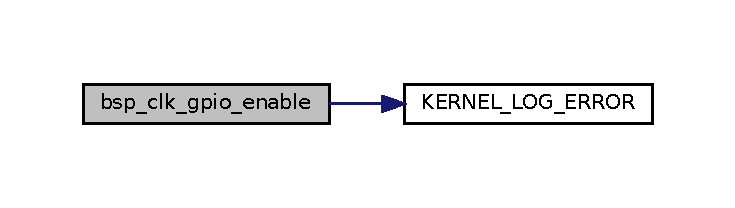
\includegraphics[width=350pt]{bsp__clocks_8h_a500b2e77b70c93b3f2b4a94cc9bcf79d_cgraph}
\end{center}
\end{figure}
Here is the caller graph for this function\+:\nopagebreak
\begin{figure}[H]
\begin{center}
\leavevmode
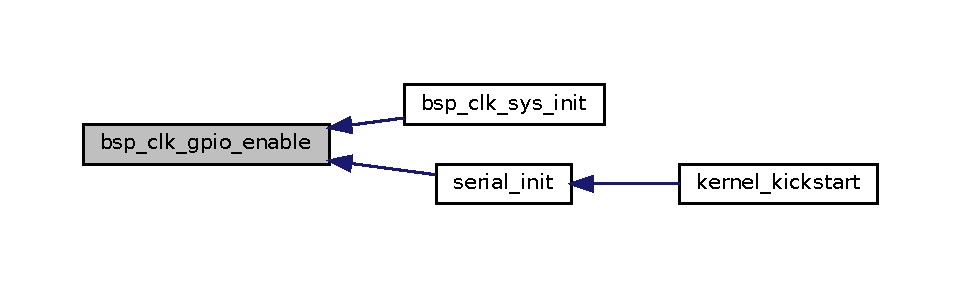
\includegraphics[width=350pt]{bsp__clocks_8h_a500b2e77b70c93b3f2b4a94cc9bcf79d_icgraph}
\end{center}
\end{figure}
\mbox{\Hypertarget{bsp__clocks_8h_a286d003315af35aa9dd72b86ba6d8420}\label{bsp__clocks_8h_a286d003315af35aa9dd72b86ba6d8420}} 
\index{bsp\+\_\+clocks.\+h@{bsp\+\_\+clocks.\+h}!bsp\+\_\+clk\+\_\+sys\+\_\+init@{bsp\+\_\+clk\+\_\+sys\+\_\+init}}
\index{bsp\+\_\+clk\+\_\+sys\+\_\+init@{bsp\+\_\+clk\+\_\+sys\+\_\+init}!bsp\+\_\+clocks.\+h@{bsp\+\_\+clocks.\+h}}
\subsubsection{\texorpdfstring{bsp\+\_\+clk\+\_\+sys\+\_\+init()}{bsp\_clk\_sys\_init()}}
{\footnotesize\ttfamily \hyperlink{error__types_8h_acf146bc98f60f47c79d782f7523e339c}{E\+R\+R\+O\+R\+\_\+\+C\+O\+D\+E\+\_\+E} bsp\+\_\+clk\+\_\+sys\+\_\+init (\begin{DoxyParamCaption}\item[{void}]{ }\end{DoxyParamCaption})}



Initializes system clocks. 

Initializes system clocks. The C\+PU, A\+HB and A\+PB clocks are initialized. The function also sets the regulator output voltage needed by the clocks.

\begin{DoxyReturn}{Returns}
N\+O\+\_\+\+E\+R\+R\+OR is returned in case of success. Otherwise an error code is returned. Please refer to the list of the standard error codes. 
\end{DoxyReturn}


Definition at line 242 of file bsp\+\_\+clocks.\+c.


\begin{DoxyCode}
243 \{
244     \hyperlink{error__types_8h_acf146bc98f60f47c79d782f7523e339c}{ERROR\_CODE\_E} error;
245 
246     \textcolor{comment}{/* Check init state */}
247     \textcolor{keywordflow}{if}(\hyperlink{bsp__clocks_8c_a7e7b4728df96b76f3a8042b7fb46aa8c}{bsp\_clk\_init} != 0)
248     \{
249 \textcolor{preprocessor}{#if KERNEL\_LOG\_LEVEL == ERROR\_LOG\_LEVEL
}
250         \hyperlink{logger_8h_a580bb63c1418b2fc8456f9b6c5b6d39d}{KERNEL\_LOG\_ERROR}(\textcolor{stringliteral}{"System clock is already initialized"}, 
251                          \hyperlink{error__types_8h_a4db9ee29f2ff83c71567c12f6bfbf28ca9af911a6ba1c32ce22213d689cb59f86}{ERROR\_ALREADY\_INIT}, 
252                          \textcolor{keyword}{sizeof}(\hyperlink{error__types_8h_a4db9ee29f2ff83c71567c12f6bfbf28ca9af911a6ba1c32ce22213d689cb59f86}{ERROR\_ALREADY\_INIT}), 
253                          \hyperlink{error__types_8h_a4db9ee29f2ff83c71567c12f6bfbf28ca9af911a6ba1c32ce22213d689cb59f86}{ERROR\_ALREADY\_INIT});
254 \textcolor{preprocessor}{#endif
}
255         \textcolor{keywordflow}{return} \hyperlink{error__types_8h_a4db9ee29f2ff83c71567c12f6bfbf28ca9af911a6ba1c32ce22213d689cb59f86}{ERROR\_ALREADY\_INIT};
256     \}
257 
258     \textcolor{comment}{/* Enable the power interface clock and system clock controller */}
259     *\hyperlink{bsp__clocks_8h_aae3fa9b2133a67e3ca65db35f8ac9a4c}{RCC\_APB1ENR\_REGISTER} = *\hyperlink{bsp__clocks_8h_aae3fa9b2133a67e3ca65db35f8ac9a4c}{RCC\_APB1ENR\_REGISTER} | 
      \hyperlink{bsp__clocks_8h_a5c19997ccd28464b80a7c3325da0ca60}{RCC\_APB1ENR\_PWREN};
260     \textcolor{keywordflow}{while}((*\hyperlink{bsp__clocks_8h_aae3fa9b2133a67e3ca65db35f8ac9a4c}{RCC\_APB1ENR\_REGISTER} & \hyperlink{bsp__clocks_8h_a5c19997ccd28464b80a7c3325da0ca60}{RCC\_APB1ENR\_PWREN}) == 0);
261     *\hyperlink{bsp__clocks_8h_aae721f66e88c2e4264580d95d5ffdd59}{RCC\_APB2ENR\_REGISTER} = *\hyperlink{bsp__clocks_8h_aae721f66e88c2e4264580d95d5ffdd59}{RCC\_APB2ENR\_REGISTER} | 
      \hyperlink{bsp__clocks_8h_a7a9d56a8aa1fa0f519ecbdf0d19dd4da}{RCC\_APB2ENR\_SYSCFGEN};
262     \textcolor{keywordflow}{while}((*\hyperlink{bsp__clocks_8h_aae721f66e88c2e4264580d95d5ffdd59}{RCC\_APB2ENR\_REGISTER} & \hyperlink{bsp__clocks_8h_a7a9d56a8aa1fa0f519ecbdf0d19dd4da}{RCC\_APB2ENR\_SYSCFGEN}) == 0);
263 
264     \textcolor{comment}{/* Update voltage scaling */}
265     error = \hyperlink{bsp__power_8h_abe4bd68d683c1ab3fbc83afb60b36ede}{bsp\_pwr\_set\_scaling}(\hyperlink{bsp__power_8h_aeab31582495468040935b45b76f06553a8ddc2bb242e2a77509aad0d808c22339}{POWER\_SCALING\_MODE\_2});
266     \textcolor{keywordflow}{if}(error != \hyperlink{error__types_8h_a4db9ee29f2ff83c71567c12f6bfbf28cabf350750d0d4fabd8954c0f1e9bbae94}{NO\_ERROR})
267     \{
268         \textcolor{keywordflow}{return} error;
269     \}
270     
271     \textcolor{comment}{/* Set flash latency */}
272     error = \hyperlink{bsp__flash_8h_a51f3c79743adab8e26ca7a5c6b33c55b}{bsp\_flash\_set\_latency}(\hyperlink{bsp__flash_8h_ad230debff3c818a6f9ced62364bc86c0ad84e36d61f83d1f0104cb3384726476c}{FLASH\_LATENCY\_WS\_2});
273     \textcolor{keywordflow}{if}(error != \hyperlink{error__types_8h_a4db9ee29f2ff83c71567c12f6bfbf28cabf350750d0d4fabd8954c0f1e9bbae94}{NO\_ERROR})
274     \{
275         \textcolor{keywordflow}{return} error;
276     \}
277 
278     \textcolor{comment}{/* Init systems clocks */}
279     \hyperlink{bsp__clocks_8c_a0ce28d57a364aa3702778c54bb4d3c05}{bsp\_clk\_base\_sys\_init}();
280     \hyperlink{bsp__clocks_8c_a1b855e007d20366749d59e4eda97222f}{bsp\_clk\_pll\_init}();
281     \hyperlink{bsp__clocks_8c_a69dea9163b1220130c719ac0b3b9327f}{bsp\_clk\_switch\_to\_pll}();
282 
283     \textcolor{comment}{/* Init GPIO and USART clocks */}
284     error = \hyperlink{bsp__clocks_8c_a500b2e77b70c93b3f2b4a94cc9bcf79d}{bsp\_clk\_gpio\_enable}(\hyperlink{bsp__gpio_8h_a69f521b579d2c761dd65949f2bae88f3a4cb73b98ec508807d984052a1598950a}{GPIO\_ID\_A});
285     \textcolor{keywordflow}{if}(error != \hyperlink{error__types_8h_a4db9ee29f2ff83c71567c12f6bfbf28cabf350750d0d4fabd8954c0f1e9bbae94}{NO\_ERROR})
286     \{
287         \textcolor{keywordflow}{return} error;
288     \}
289     error = \hyperlink{bsp__clocks_8c_aaf01af602e17579af5e6af009ae7a557}{bsp\_clk\_usart\_enable}(\hyperlink{bsp__usart_8h_a58f9be3820e29e0fbf00e2466c3ee768abb138542d801249fd01ec62c34f52cff}{USART\_ID\_2});
290     \textcolor{keywordflow}{if}(error != \hyperlink{error__types_8h_a4db9ee29f2ff83c71567c12f6bfbf28cabf350750d0d4fabd8954c0f1e9bbae94}{NO\_ERROR})
291     \{
292         \textcolor{keywordflow}{return} error;
293     \}
294 
295 \textcolor{preprocessor}{#if KERNEL\_LOG\_LEVEL >= INFO\_LOG\_LEVEL
}
296     KERNEL\_LOG\_INFO(\textcolor{stringliteral}{"System clock initialized"}, 
297                     \hyperlink{error__types_8h_a4db9ee29f2ff83c71567c12f6bfbf28cabf350750d0d4fabd8954c0f1e9bbae94}{NO\_ERROR}, 
298                     \textcolor{keyword}{sizeof}(\hyperlink{error__types_8h_a4db9ee29f2ff83c71567c12f6bfbf28cabf350750d0d4fabd8954c0f1e9bbae94}{NO\_ERROR}), 
299                     \hyperlink{error__types_8h_a4db9ee29f2ff83c71567c12f6bfbf28cabf350750d0d4fabd8954c0f1e9bbae94}{NO\_ERROR});
300 \textcolor{preprocessor}{#endif
}
301 
302     \textcolor{comment}{/* Update init state */}
303     \hyperlink{bsp__clocks_8c_a7e7b4728df96b76f3a8042b7fb46aa8c}{bsp\_clk\_init} = 1;
304     \textcolor{keywordflow}{return} \hyperlink{error__types_8h_a4db9ee29f2ff83c71567c12f6bfbf28cabf350750d0d4fabd8954c0f1e9bbae94}{NO\_ERROR};
305 \}
\end{DoxyCode}
Here is the call graph for this function\+:\nopagebreak
\begin{figure}[H]
\begin{center}
\leavevmode
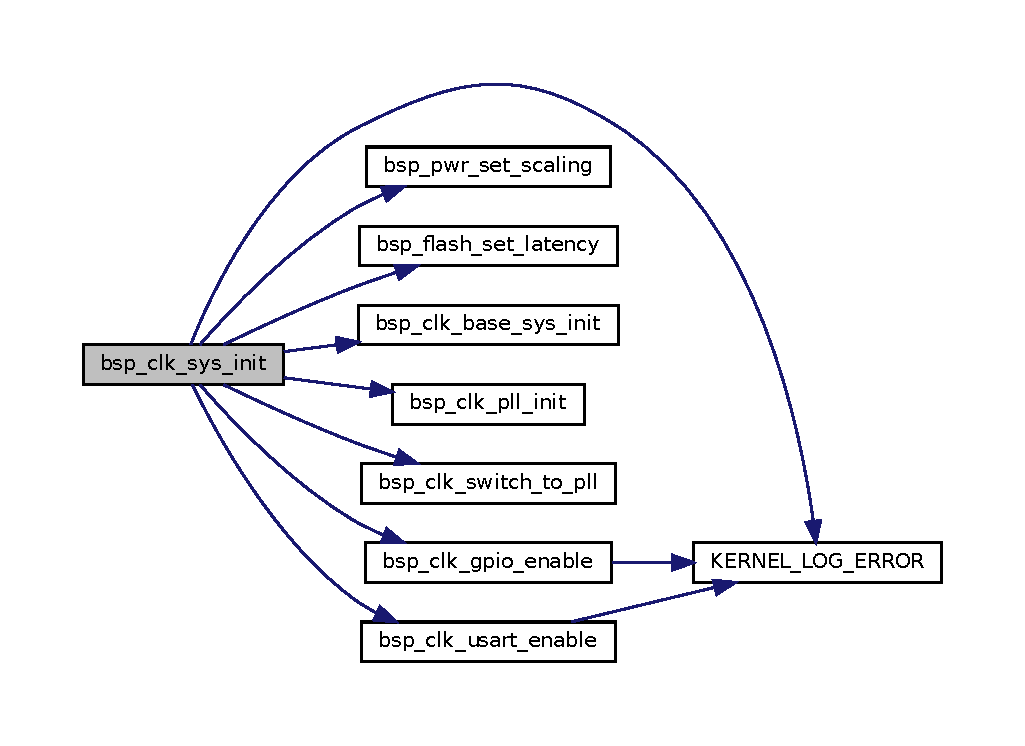
\includegraphics[width=350pt]{bsp__clocks_8h_a286d003315af35aa9dd72b86ba6d8420_cgraph}
\end{center}
\end{figure}
\mbox{\Hypertarget{bsp__clocks_8h_aaf01af602e17579af5e6af009ae7a557}\label{bsp__clocks_8h_aaf01af602e17579af5e6af009ae7a557}} 
\index{bsp\+\_\+clocks.\+h@{bsp\+\_\+clocks.\+h}!bsp\+\_\+clk\+\_\+usart\+\_\+enable@{bsp\+\_\+clk\+\_\+usart\+\_\+enable}}
\index{bsp\+\_\+clk\+\_\+usart\+\_\+enable@{bsp\+\_\+clk\+\_\+usart\+\_\+enable}!bsp\+\_\+clocks.\+h@{bsp\+\_\+clocks.\+h}}
\subsubsection{\texorpdfstring{bsp\+\_\+clk\+\_\+usart\+\_\+enable()}{bsp\_clk\_usart\_enable()}}
{\footnotesize\ttfamily \hyperlink{error__types_8h_acf146bc98f60f47c79d782f7523e339c}{E\+R\+R\+O\+R\+\_\+\+C\+O\+D\+E\+\_\+E} bsp\+\_\+clk\+\_\+usart\+\_\+enable (\begin{DoxyParamCaption}\item[{const \hyperlink{bsp__usart_8h_a594f9d90a9a3875660da4512fb208cf9}{U\+S\+A\+R\+T\+\_\+\+I\+D\+E\+N\+T\+I\+F\+I\+E\+R\+\_\+E}}]{usart\+\_\+id }\end{DoxyParamCaption})}



Enables the U\+S\+A\+RT clocks. 

Enables the U\+S\+A\+RT clocks. This function will enable the peripheral clock used by the U\+S\+A\+RT corresponding to the identifier given as parameter. If the identifier is unknown, the function has no effect.


\begin{DoxyParams}[1]{Parameters}
\mbox{\tt in}  & {\em usart\+\_\+id} & The U\+S\+A\+RT identifier for which the clock should be enabled.\\
\hline
\end{DoxyParams}
\begin{DoxyReturn}{Returns}
N\+O\+\_\+\+E\+R\+R\+OR is returned in case of success. Otherwise an error code is returned. Please refer to the list of the standard error codes. 
\end{DoxyReturn}


Definition at line 197 of file bsp\+\_\+clocks.\+c.


\begin{DoxyCode}
198 \{
199     \hyperlink{error__types_8h_acf146bc98f60f47c79d782f7523e339c}{ERROR\_CODE\_E} error;
200 
201     error = \hyperlink{error__types_8h_a4db9ee29f2ff83c71567c12f6bfbf28cabf350750d0d4fabd8954c0f1e9bbae94}{NO\_ERROR};
202 
203     \textcolor{comment}{/* Select the USART interface */}
204     \textcolor{keywordflow}{switch}(usart\_id)
205     \{
206         \textcolor{keywordflow}{case} \hyperlink{bsp__usart_8h_a58f9be3820e29e0fbf00e2466c3ee768a512d550c862eac9ad45d923508bb0f7d}{USART\_ID\_1}:
207             *\hyperlink{bsp__clocks_8h_aae721f66e88c2e4264580d95d5ffdd59}{RCC\_APB2ENR\_REGISTER} = *\hyperlink{bsp__clocks_8h_aae721f66e88c2e4264580d95d5ffdd59}{RCC\_APB2ENR\_REGISTER} | 
208                                      \hyperlink{bsp__clocks_8h_a4666bb90842e8134b32e6a34a0f165f3}{RCC\_APB2ENR\_USART1EN};
209             \textcolor{keywordflow}{while}((*\hyperlink{bsp__clocks_8h_aae721f66e88c2e4264580d95d5ffdd59}{RCC\_APB2ENR\_REGISTER} & 
      \hyperlink{bsp__clocks_8h_a4666bb90842e8134b32e6a34a0f165f3}{RCC\_APB2ENR\_USART1EN}) == 0);
210             \textcolor{keywordflow}{break};
211         \textcolor{keywordflow}{case} \hyperlink{bsp__usart_8h_a58f9be3820e29e0fbf00e2466c3ee768abb138542d801249fd01ec62c34f52cff}{USART\_ID\_2}:
212             *\hyperlink{bsp__clocks_8h_aae3fa9b2133a67e3ca65db35f8ac9a4c}{RCC\_APB1ENR\_REGISTER} = *\hyperlink{bsp__clocks_8h_aae3fa9b2133a67e3ca65db35f8ac9a4c}{RCC\_APB1ENR\_REGISTER} | 
213                                      \hyperlink{bsp__clocks_8h_ab840af4f735ec36419d61c7db3cfa00d}{RCC\_APB1ENR\_USART2EN};
214             \textcolor{keywordflow}{while}((*\hyperlink{bsp__clocks_8h_aae3fa9b2133a67e3ca65db35f8ac9a4c}{RCC\_APB1ENR\_REGISTER} & 
      \hyperlink{bsp__clocks_8h_ab840af4f735ec36419d61c7db3cfa00d}{RCC\_APB1ENR\_USART2EN}) == 0);
215             \textcolor{keywordflow}{break};
216         \textcolor{keywordflow}{case} \hyperlink{bsp__usart_8h_a58f9be3820e29e0fbf00e2466c3ee768afd45e5de3678cbcada70f46bde327479}{USART\_ID\_6}:
217             *\hyperlink{bsp__clocks_8h_aae721f66e88c2e4264580d95d5ffdd59}{RCC\_APB2ENR\_REGISTER} = *\hyperlink{bsp__clocks_8h_aae721f66e88c2e4264580d95d5ffdd59}{RCC\_APB2ENR\_REGISTER} | 
218                                      \hyperlink{bsp__clocks_8h_a0569d91f3b18ae130b7a09e0100c4459}{RCC\_APB2ENR\_USART6EN};
219             \textcolor{keywordflow}{while}((*\hyperlink{bsp__clocks_8h_aae721f66e88c2e4264580d95d5ffdd59}{RCC\_APB2ENR\_REGISTER} & 
      \hyperlink{bsp__clocks_8h_a0569d91f3b18ae130b7a09e0100c4459}{RCC\_APB2ENR\_USART6EN}) == 0);
220             \textcolor{keywordflow}{break};
221 
222         \textcolor{keywordflow}{default}:
223 \textcolor{preprocessor}{#if KERNEL\_LOG\_LEVEL == ERROR\_LOG\_LEVEL
}
224             \hyperlink{logger_8h_a580bb63c1418b2fc8456f9b6c5b6d39d}{KERNEL\_LOG\_ERROR}(\textcolor{stringliteral}{"Wrong USART identifer"}, 
225                             usart\_id, 
226                             \textcolor{keyword}{sizeof}(usart\_id), 
227                             \hyperlink{error__types_8h_a4db9ee29f2ff83c71567c12f6bfbf28cabbe6797281350f36c23d07d6f2d7f6e2}{ERROR\_INVALID\_PARAM});
228 \textcolor{preprocessor}{#endif
}
229             error = \hyperlink{error__types_8h_a4db9ee29f2ff83c71567c12f6bfbf28cabbe6797281350f36c23d07d6f2d7f6e2}{ERROR\_INVALID\_PARAM};
230     \}
231 
232 \textcolor{preprocessor}{#if KERNEL\_LOG\_LEVEL >= INFO\_LOG\_LEVEL
}
233     KERNEL\_LOG\_INFO(\textcolor{stringliteral}{"USART clock enabled"}, 
234                     usart\_id, 
235                     \textcolor{keyword}{sizeof}(usart\_id), 
236                     \hyperlink{error__types_8h_a4db9ee29f2ff83c71567c12f6bfbf28cabf350750d0d4fabd8954c0f1e9bbae94}{NO\_ERROR});
237 \textcolor{preprocessor}{#endif
}
238 
239     \textcolor{keywordflow}{return} error;
240 \}
\end{DoxyCode}
Here is the call graph for this function\+:\nopagebreak
\begin{figure}[H]
\begin{center}
\leavevmode
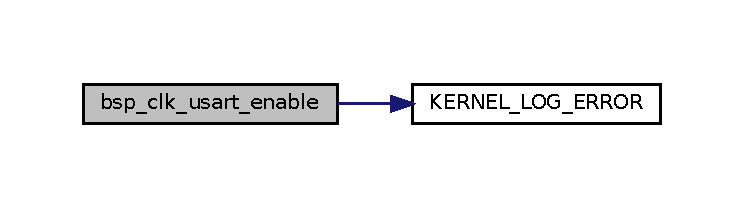
\includegraphics[width=350pt]{bsp__clocks_8h_aaf01af602e17579af5e6af009ae7a557_cgraph}
\end{center}
\end{figure}
Here is the caller graph for this function\+:\nopagebreak
\begin{figure}[H]
\begin{center}
\leavevmode
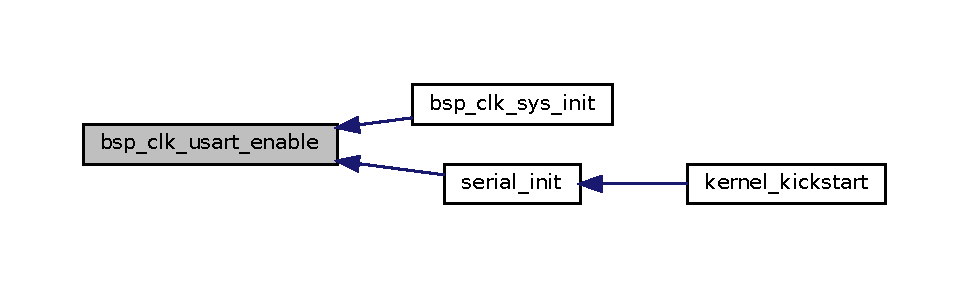
\includegraphics[width=350pt]{bsp__clocks_8h_aaf01af602e17579af5e6af009ae7a557_icgraph}
\end{center}
\end{figure}
\mbox{\Hypertarget{bsp__clocks_8h_aeeded4b587684fa3383b3d42ee29af1e}\label{bsp__clocks_8h_aeeded4b587684fa3383b3d42ee29af1e}} 
\index{bsp\+\_\+clocks.\+h@{bsp\+\_\+clocks.\+h}!bsp\+\_\+clocks\+\_\+get\+\_\+freq@{bsp\+\_\+clocks\+\_\+get\+\_\+freq}}
\index{bsp\+\_\+clocks\+\_\+get\+\_\+freq@{bsp\+\_\+clocks\+\_\+get\+\_\+freq}!bsp\+\_\+clocks.\+h@{bsp\+\_\+clocks.\+h}}
\subsubsection{\texorpdfstring{bsp\+\_\+clocks\+\_\+get\+\_\+freq()}{bsp\_clocks\_get\_freq()}}
{\footnotesize\ttfamily \hyperlink{stdint_8h_a324c5d28c0d82f502a234ab99efac87a}{uint32\+\_\+t} bsp\+\_\+clocks\+\_\+get\+\_\+freq (\begin{DoxyParamCaption}\item[{const \hyperlink{bsp__clocks_8h_ac9d4d589a659370f313ef156f6eff0e8}{C\+L\+O\+C\+K\+\_\+\+I\+D\+E\+N\+T\+I\+F\+I\+E\+R\+\_\+T}}]{clk\+\_\+id }\end{DoxyParamCaption})}



Get the frequencies in M\+Hz of the clocks which identifer corresponds to the identifier given as parameter. 

Get the frequencies of the clocks which identifer corresponds to the identifier given as parameter. The P\+LL parameters and other clocks register are read to return the correct frequency for a given clock.


\begin{DoxyParams}[1]{Parameters}
\mbox{\tt in}  & {\em clk\+\_\+id} & The identifier of the clock.\\
\hline
\end{DoxyParams}
\begin{DoxyReturn}{Returns}
The frequency in M\+Hz of the clock is returned. 
\end{DoxyReturn}


Definition at line 307 of file bsp\+\_\+clocks.\+c.


\begin{DoxyCode}
308 \{
309     \hyperlink{stdint_8h_a324c5d28c0d82f502a234ab99efac87a}{uint32\_t} sysclk;
310     \hyperlink{stdint_8h_a324c5d28c0d82f502a234ab99efac87a}{uint32\_t} factor;
311 
312     \textcolor{comment}{/* Get Source clock */}
313     \textcolor{keywordflow}{if}((*\hyperlink{bsp__clocks_8h_ac454715dd9c4f8ba957cc53f318c58ac}{RCC\_CFGR\_REGISTER} & \hyperlink{bsp__clocks_8h_a451045d952eb1caaa0090c9e8dc75082}{RCC\_CFGR\_SWS\_MASK}) == 
      \hyperlink{bsp__clocks_8h_a2c67e2279804a83ef24438267d9d4a6c}{RCC\_CFGR\_SWS\_PLL})
314     \{
315         sysclk = \hyperlink{bsp__clocks_8c_ac154ab5d2a56dd8e09e0545e9775112e}{bsp\_clock\_get\_pll\_freq}();
316     \}
317     \textcolor{keywordflow}{else} \textcolor{keywordflow}{if}((*\hyperlink{bsp__clocks_8h_ac454715dd9c4f8ba957cc53f318c58ac}{RCC\_CFGR\_REGISTER} & RCC\_CFGR\_SWS\_MASK) == 
      \hyperlink{bsp__clocks_8h_a6764639cf221e1ebc0b5448dcaed590a}{RCC\_CFGR\_SWS\_HSI})
318     \{
319         sysclk = \hyperlink{bsp__clocks_8h_ae89e6b2d1e86b7fb4831cb013ece2c52}{RCC\_HSI\_BASE\_FREQ};
320     \}
321     \textcolor{keywordflow}{else} \textcolor{keywordflow}{if}((*\hyperlink{bsp__clocks_8h_ac454715dd9c4f8ba957cc53f318c58ac}{RCC\_CFGR\_REGISTER} & RCC\_CFGR\_SWS\_MASK) == 
      \hyperlink{bsp__clocks_8h_ae09a0202f441c1a43e69c62331d50a08}{RCC\_CFGR\_SWS\_HSE})
322     \{
323         sysclk = \hyperlink{bsp__clocks_8h_a19d723f47200a1da259e9c147f2de258}{RCC\_HSE\_BASE\_FREQ};
324     \}
325     \textcolor{keywordflow}{else} 
326     \{
327         \textcolor{comment}{/* We were  not able to detect the input clock */}
328         \textcolor{keywordflow}{return} 0;
329     \}
330 
331     \textcolor{comment}{/* Divide by AHB prescaler */}
332     \textcolor{keywordflow}{if}((*\hyperlink{bsp__clocks_8h_ac454715dd9c4f8ba957cc53f318c58ac}{RCC\_CFGR\_REGISTER} & \hyperlink{bsp__clocks_8h_a1351ccf5f6a5d9a6b91c4f533688d8fb}{RCC\_CFGR\_HPRE\_EN}) != 0)
333     \{
334         factor = (*\hyperlink{bsp__clocks_8h_ac454715dd9c4f8ba957cc53f318c58ac}{RCC\_CFGR\_REGISTER} & \hyperlink{bsp__clocks_8h_a2ff38fa14905e578752b706e5c29b146}{RCC\_CFGR\_HPRE\_VAL\_MASK}) >> 
335                   \hyperlink{bsp__clocks_8h_adca5b474c16bb5c9b4bbedfabeba8e25}{RCC\_CFGR\_HRPE\_OFFSET};
336         sysclk /= (\hyperlink{stdint_8h_a324c5d28c0d82f502a234ab99efac87a}{uint32\_t})\hyperlink{bsp__clocks_8c_abed7da9c2bfa6c8191c3bf928e64041f}{bsp\_hpre\_factor\_lookup}[factor];
337     \}
338 
339     \textcolor{keywordflow}{if}(clk\_id == \hyperlink{bsp__clocks_8h_ad0e92b49c1a7205e3460ca1e54fa9d70a58357d0569548d6c2ba44f27e0aa6ba6}{BSP\_CLOCK\_ID\_HCLK} || clk\_id == 
      \hyperlink{bsp__clocks_8h_ad0e92b49c1a7205e3460ca1e54fa9d70a265c9dec4478eb66904a2dbc6954e598}{BSP\_CLOCK\_ID\_FCLK})
340     \{
341         \textcolor{keywordflow}{return} sysclk;
342     \}
343     \textcolor{keywordflow}{else} \textcolor{keywordflow}{if}(clk\_id == \hyperlink{bsp__clocks_8h_ad0e92b49c1a7205e3460ca1e54fa9d70a0493d0bbd7edf1aebadb342c5c38f709}{BSP\_CLOCK\_ID\_PCLK1} || clk\_id == 
      \hyperlink{bsp__clocks_8h_ad0e92b49c1a7205e3460ca1e54fa9d70aad46d3b8852f9a4d711c15164bf1c0d3}{BSP\_CLOCK\_ID\_APB1\_TIMER})
344     \{
345         \textcolor{comment}{/* Get the APB1 prescaler */}
346         \textcolor{keywordflow}{if}((*\hyperlink{bsp__clocks_8h_ac454715dd9c4f8ba957cc53f318c58ac}{RCC\_CFGR\_REGISTER} & \hyperlink{bsp__clocks_8h_a7a4503de78658d3271cb5494adc96e41}{RCC\_CFGR\_PPRE1\_EN}) != 0)
347         \{
348             factor = (*\hyperlink{bsp__clocks_8h_ac454715dd9c4f8ba957cc53f318c58ac}{RCC\_CFGR\_REGISTER} & 
      \hyperlink{bsp__clocks_8h_aebda6f102f65bc354b95232527021aba}{RCC\_CFGR\_PPRE1\_VAL\_MASK}) >> 
349                       \hyperlink{bsp__clocks_8h_a1f605f808c9ab7530142dd8808e83a22}{RCC\_CFGR\_PPRE1\_OFFSET};
350 
351             sysclk /= (\hyperlink{stdint_8h_a324c5d28c0d82f502a234ab99efac87a}{uint32\_t})\hyperlink{bsp__clocks_8c_a1ef2cd1399c95dbe65a524595da1fc5c}{bsp\_ppre\_factor\_lookup}[factor];
352 
353             \textcolor{keywordflow}{if}(clk\_id == \hyperlink{bsp__clocks_8h_ad0e92b49c1a7205e3460ca1e54fa9d70aad46d3b8852f9a4d711c15164bf1c0d3}{BSP\_CLOCK\_ID\_APB1\_TIMER})
354             \{
355                 sysclk *= 2;
356             \}
357         \}
358     \}
359     \textcolor{keywordflow}{else} \textcolor{keywordflow}{if}(clk\_id == \hyperlink{bsp__clocks_8h_ad0e92b49c1a7205e3460ca1e54fa9d70aad62d8c78d2b4617724a82ec190a33ee}{BSP\_CLOCK\_ID\_PCLK2} || clk\_id == 
      \hyperlink{bsp__clocks_8h_ad0e92b49c1a7205e3460ca1e54fa9d70a30cca3be6a7bad72d2c02e9b58ff4d50}{BSP\_CLOCK\_ID\_APB2\_TIMER})
360     \{
361         \textcolor{comment}{/* Get the APB2 prescaler */}
362         \textcolor{keywordflow}{if}((*\hyperlink{bsp__clocks_8h_ac454715dd9c4f8ba957cc53f318c58ac}{RCC\_CFGR\_REGISTER} & \hyperlink{bsp__clocks_8h_a1a384b58d9f246cb60ed0d0bfa92cbf4}{RCC\_CFGR\_PPRE2\_EN}) != 0)
363         \{
364             factor = (*\hyperlink{bsp__clocks_8h_ac454715dd9c4f8ba957cc53f318c58ac}{RCC\_CFGR\_REGISTER} & 
      \hyperlink{bsp__clocks_8h_adb27fe14c6c6c2cb20f13aaf86f0900a}{RCC\_CFGR\_PPRE2\_VAL\_MASK}) >> 
365                       \hyperlink{bsp__clocks_8h_a906e390883db586903c4b1144a182e47}{RCC\_CFGR\_PPRE2\_OFFSET};
366             sysclk /= \hyperlink{bsp__clocks_8c_a1ef2cd1399c95dbe65a524595da1fc5c}{bsp\_ppre\_factor\_lookup}[factor];
367 
368             \textcolor{keywordflow}{if}(clk\_id == \hyperlink{bsp__clocks_8h_ad0e92b49c1a7205e3460ca1e54fa9d70a30cca3be6a7bad72d2c02e9b58ff4d50}{BSP\_CLOCK\_ID\_APB2\_TIMER})
369             \{
370                 sysclk *= 2;
371             \}
372         \}
373     \}
374     \textcolor{keywordflow}{else} 
375     \{
376         sysclk = 0;
377     \}
378 
379 \textcolor{preprocessor}{#if KERNEL\_LOG\_LEVEL >= INFO\_LOG\_LEVEL
}
380     KERNEL\_LOG\_INFO(\textcolor{stringliteral}{"System clock frequency requested"}, 
381                     (\textcolor{keywordtype}{void}*)(\hyperlink{stdint_8h_a324c5d28c0d82f502a234ab99efac87a}{uint32\_t})sysclk, 
382                     \textcolor{keyword}{sizeof}(sysclk), 
383                     \hyperlink{error__types_8h_a4db9ee29f2ff83c71567c12f6bfbf28cabf350750d0d4fabd8954c0f1e9bbae94}{NO\_ERROR});
384 \textcolor{preprocessor}{#endif
}
385 
386     \textcolor{keywordflow}{return} sysclk;
387 \}
\end{DoxyCode}
Here is the call graph for this function\+:
\nopagebreak
\begin{figure}[H]
\begin{center}
\leavevmode
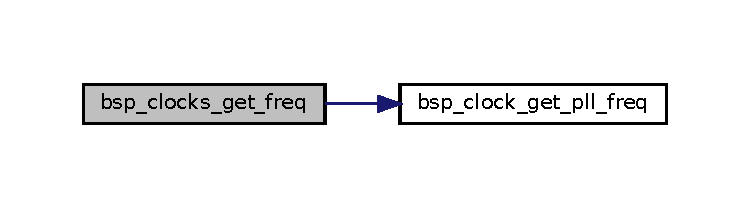
\includegraphics[width=350pt]{bsp__clocks_8h_aeeded4b587684fa3383b3d42ee29af1e_cgraph}
\end{center}
\end{figure}
Here is the caller graph for this function\+:
\nopagebreak
\begin{figure}[H]
\begin{center}
\leavevmode
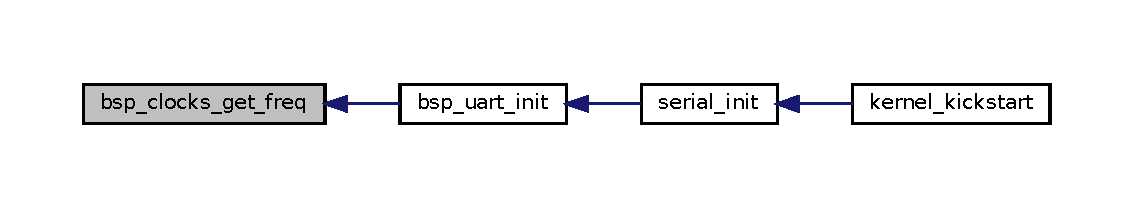
\includegraphics[width=350pt]{bsp__clocks_8h_aeeded4b587684fa3383b3d42ee29af1e_icgraph}
\end{center}
\end{figure}

\hypertarget{bsp__flash_8h}{}\section{Kernel/\+Sources/arch/board/stm32/f401re/includes/bsp\+\_\+flash.h File Reference}
\label{bsp__flash_8h}\index{Kernel/\+Sources/arch/board/stm32/f401re/includes/bsp\+\_\+flash.\+h@{Kernel/\+Sources/arch/board/stm32/f401re/includes/bsp\+\_\+flash.\+h}}
{\ttfamily \#include \char`\"{}error\+\_\+types.\+h\char`\"{}}\newline
{\ttfamily \#include \char`\"{}stdint.\+h\char`\"{}}\newline
Include dependency graph for bsp\+\_\+flash.\+h\+:\nopagebreak
\begin{figure}[H]
\begin{center}
\leavevmode
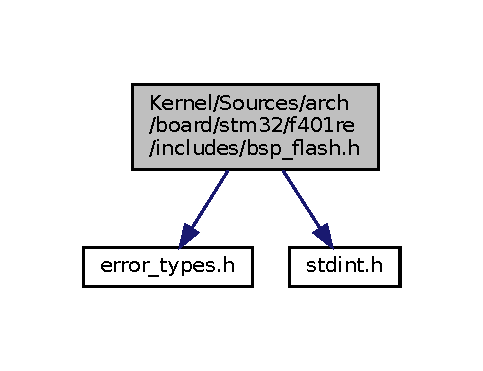
\includegraphics[width=232pt]{bsp__flash_8h__incl}
\end{center}
\end{figure}
This graph shows which files directly or indirectly include this file\+:\nopagebreak
\begin{figure}[H]
\begin{center}
\leavevmode
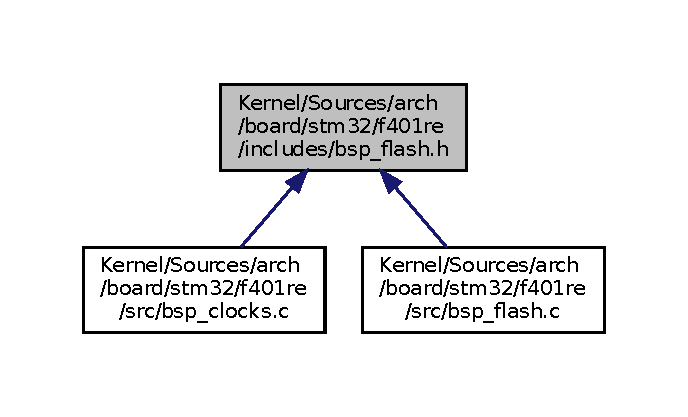
\includegraphics[width=330pt]{bsp__flash_8h__dep__incl}
\end{center}
\end{figure}
\subsection*{Macros}
\begin{DoxyCompactItemize}
\item 
\#define \hyperlink{bsp__flash_8h_a1c4f0bbe8f3dc074a0df26f8759ca632}{F\+L\+A\+S\+H\+\_\+\+A\+C\+R\+\_\+\+A\+D\+D\+R\+E\+SS}~0x40023\+C00
\begin{DoxyCompactList}\small\item\em Flash Access Control Register address. \end{DoxyCompactList}\item 
\#define \hyperlink{bsp__flash_8h_a177b682ed269b91b61bf46005fca9620}{F\+L\+A\+S\+H\+\_\+\+A\+C\+R\+\_\+\+R\+E\+G\+I\+S\+T\+ER}~((volatile \hyperlink{stdint_8h_a324c5d28c0d82f502a234ab99efac87a}{uint32\+\_\+t}$\ast$)\hyperlink{bsp__flash_8h_a1c4f0bbe8f3dc074a0df26f8759ca632}{F\+L\+A\+S\+H\+\_\+\+A\+C\+R\+\_\+\+A\+D\+D\+R\+E\+SS})
\item 
\#define \hyperlink{bsp__flash_8h_a941d0c7a25f08c35724c4a572d90a6cc}{F\+L\+A\+S\+H\+\_\+\+A\+C\+R\+\_\+\+D\+C\+A\+C\+H\+E\+\_\+\+EN}~0x00000400
\begin{DoxyCompactList}\small\item\em Flash data cache enable bit. \end{DoxyCompactList}\item 
\#define \hyperlink{bsp__flash_8h_a8723e738daa1eb5acfd3d66130060541}{F\+L\+A\+S\+H\+\_\+\+A\+C\+R\+\_\+\+I\+C\+A\+C\+H\+E\+\_\+\+EN}~0x00000200
\begin{DoxyCompactList}\small\item\em Flash instruction cache enable bit. \end{DoxyCompactList}\item 
\#define \hyperlink{bsp__flash_8h_a479a3f068bb372bdf3bfc5b37846378a}{F\+L\+A\+S\+H\+\_\+\+A\+C\+R\+\_\+\+P\+R\+E\+F\+E\+T\+C\+H\+\_\+\+EN}~0x00000100
\begin{DoxyCompactList}\small\item\em Flash prefetch enable bit. \end{DoxyCompactList}\item 
\#define \hyperlink{bsp__flash_8h_a325fd0108f2a85889c495a9f08409216}{F\+L\+A\+S\+H\+\_\+\+A\+C\+R\+\_\+\+L\+A\+T\+E\+N\+C\+Y\+\_\+\+M\+A\+SK}~0x0000000F
\begin{DoxyCompactList}\small\item\em Flash A\+CR latency mask. \end{DoxyCompactList}\end{DoxyCompactItemize}
\subsection*{Typedefs}
\begin{DoxyCompactItemize}
\item 
typedef enum \hyperlink{bsp__flash_8h_ad230debff3c818a6f9ced62364bc86c0}{F\+L\+A\+S\+H\+\_\+\+L\+A\+T\+E\+N\+C\+Y\+\_\+\+WS} \hyperlink{bsp__flash_8h_ab4bdf422e30b864e1ff48788fbde702d}{F\+L\+A\+S\+H\+\_\+\+L\+A\+T\+E\+N\+C\+Y\+\_\+\+W\+S\+\_\+E}
\begin{DoxyCompactList}\small\item\em Short hand for enum F\+L\+A\+S\+H\+\_\+\+L\+A\+T\+E\+N\+C\+Y\+\_\+\+WS. \end{DoxyCompactList}\end{DoxyCompactItemize}
\subsection*{Enumerations}
\begin{DoxyCompactItemize}
\item 
enum \hyperlink{bsp__flash_8h_ad230debff3c818a6f9ced62364bc86c0}{F\+L\+A\+S\+H\+\_\+\+L\+A\+T\+E\+N\+C\+Y\+\_\+\+WS} \{ \newline
\hyperlink{bsp__flash_8h_ad230debff3c818a6f9ced62364bc86c0a6b1ee670fc8092f3529257c6c0c31425}{F\+L\+A\+S\+H\+\_\+\+L\+A\+T\+E\+N\+C\+Y\+\_\+\+W\+S\+\_\+0} = 0x00000000, 
\hyperlink{bsp__flash_8h_ad230debff3c818a6f9ced62364bc86c0a586bfab5ee031668bf3c80fb4f8f041e}{F\+L\+A\+S\+H\+\_\+\+L\+A\+T\+E\+N\+C\+Y\+\_\+\+W\+S\+\_\+1} = 0x00000001, 
\hyperlink{bsp__flash_8h_ad230debff3c818a6f9ced62364bc86c0ad84e36d61f83d1f0104cb3384726476c}{F\+L\+A\+S\+H\+\_\+\+L\+A\+T\+E\+N\+C\+Y\+\_\+\+W\+S\+\_\+2} = 0x00000002, 
\hyperlink{bsp__flash_8h_ad230debff3c818a6f9ced62364bc86c0adee4150a2706b69d72fa73e07998c0f0}{F\+L\+A\+S\+H\+\_\+\+L\+A\+T\+E\+N\+C\+Y\+\_\+\+W\+S\+\_\+3} = 0x00000003, 
\newline
\hyperlink{bsp__flash_8h_ad230debff3c818a6f9ced62364bc86c0a36c9cd3b0de4f2ce9dcb7662f788fcbc}{F\+L\+A\+S\+H\+\_\+\+L\+A\+T\+E\+N\+C\+Y\+\_\+\+W\+S\+\_\+4} = 0x00000004, 
\hyperlink{bsp__flash_8h_ad230debff3c818a6f9ced62364bc86c0a5860994f2c5d37391c5d250160a4099b}{F\+L\+A\+S\+H\+\_\+\+L\+A\+T\+E\+N\+C\+Y\+\_\+\+W\+S\+\_\+5} = 0x00000005, 
\hyperlink{bsp__flash_8h_ad230debff3c818a6f9ced62364bc86c0a794d4d821afca5acd940b48f5d0272ca}{F\+L\+A\+S\+H\+\_\+\+L\+A\+T\+E\+N\+C\+Y\+\_\+\+W\+S\+\_\+6} = 0x00000006, 
\hyperlink{bsp__flash_8h_ad230debff3c818a6f9ced62364bc86c0afec2eafcf5a835005ea9b504b3cc595e}{F\+L\+A\+S\+H\+\_\+\+L\+A\+T\+E\+N\+C\+Y\+\_\+\+W\+S\+\_\+7} = 0x00000007, 
\newline
\hyperlink{bsp__flash_8h_ad230debff3c818a6f9ced62364bc86c0a740cc788e38e0123f15399c190b4d77f}{F\+L\+A\+S\+H\+\_\+\+L\+A\+T\+E\+N\+C\+Y\+\_\+\+W\+S\+\_\+8} = 0x00000008, 
\hyperlink{bsp__flash_8h_ad230debff3c818a6f9ced62364bc86c0aa1480d957f9e3d3f61e68360bb8af996}{F\+L\+A\+S\+H\+\_\+\+L\+A\+T\+E\+N\+C\+Y\+\_\+\+W\+S\+\_\+9} = 0x00000009, 
\hyperlink{bsp__flash_8h_ad230debff3c818a6f9ced62364bc86c0a94fc00df64e576cb2c0f0c2ff1e2b0f3}{F\+L\+A\+S\+H\+\_\+\+L\+A\+T\+E\+N\+C\+Y\+\_\+\+W\+S\+\_\+10} = 0x00000010, 
\hyperlink{bsp__flash_8h_ad230debff3c818a6f9ced62364bc86c0ae57f7cf478f27e92c7a7525ddc9a0540}{F\+L\+A\+S\+H\+\_\+\+L\+A\+T\+E\+N\+C\+Y\+\_\+\+W\+S\+\_\+11} = 0x00000011, 
\newline
\hyperlink{bsp__flash_8h_ad230debff3c818a6f9ced62364bc86c0a227a3e8870c7edc58a5745038a26bfc7}{F\+L\+A\+S\+H\+\_\+\+L\+A\+T\+E\+N\+C\+Y\+\_\+\+W\+S\+\_\+12} = 0x00000012, 
\hyperlink{bsp__flash_8h_ad230debff3c818a6f9ced62364bc86c0a844598c6148a81231ae693d9ad3f3b0a}{F\+L\+A\+S\+H\+\_\+\+L\+A\+T\+E\+N\+C\+Y\+\_\+\+W\+S\+\_\+13} = 0x00000013, 
\hyperlink{bsp__flash_8h_ad230debff3c818a6f9ced62364bc86c0ad970edc7e0e303f57c7c738f861d48ea}{F\+L\+A\+S\+H\+\_\+\+L\+A\+T\+E\+N\+C\+Y\+\_\+\+W\+S\+\_\+14} = 0x00000014, 
\hyperlink{bsp__flash_8h_ad230debff3c818a6f9ced62364bc86c0a453a0454c5d9669a4fa8f3a3e0de8625}{F\+L\+A\+S\+H\+\_\+\+L\+A\+T\+E\+N\+C\+Y\+\_\+\+W\+S\+\_\+15} = 0x00000015
 \}\begin{DoxyCompactList}\small\item\em Power scaling modes available on the S\+T\+M32\+F401\+RE. \end{DoxyCompactList}
\end{DoxyCompactItemize}
\subsection*{Functions}
\begin{DoxyCompactItemize}
\item 
void \hyperlink{bsp__flash_8h_a28b133b49a8b54580ef07cc2b02b6a2d}{bsp\+\_\+flash\+\_\+cache\+\_\+enable} (void)
\begin{DoxyCompactList}\small\item\em Enables flash instruction and data cache. \end{DoxyCompactList}\item 
void \hyperlink{bsp__flash_8h_a2f8e8bffdc14c9ea45296defed4606a6}{bsp\+\_\+flash\+\_\+prefetch\+\_\+enable} (void)
\begin{DoxyCompactList}\small\item\em Enables flash prefetech unit. \end{DoxyCompactList}\item 
\hyperlink{error__types_8h_acf146bc98f60f47c79d782f7523e339c}{E\+R\+R\+O\+R\+\_\+\+C\+O\+D\+E\+\_\+E} \hyperlink{bsp__flash_8h_a51f3c79743adab8e26ca7a5c6b33c55b}{bsp\+\_\+flash\+\_\+set\+\_\+latency} (const \hyperlink{bsp__flash_8h_ab4bdf422e30b864e1ff48788fbde702d}{F\+L\+A\+S\+H\+\_\+\+L\+A\+T\+E\+N\+C\+Y\+\_\+\+W\+S\+\_\+E} latency)
\begin{DoxyCompactList}\small\item\em Sets the flash latency. \end{DoxyCompactList}\end{DoxyCompactItemize}


\subsection{Macro Definition Documentation}
\mbox{\Hypertarget{bsp__flash_8h_a1c4f0bbe8f3dc074a0df26f8759ca632}\label{bsp__flash_8h_a1c4f0bbe8f3dc074a0df26f8759ca632}} 
\index{bsp\+\_\+flash.\+h@{bsp\+\_\+flash.\+h}!F\+L\+A\+S\+H\+\_\+\+A\+C\+R\+\_\+\+A\+D\+D\+R\+E\+SS@{F\+L\+A\+S\+H\+\_\+\+A\+C\+R\+\_\+\+A\+D\+D\+R\+E\+SS}}
\index{F\+L\+A\+S\+H\+\_\+\+A\+C\+R\+\_\+\+A\+D\+D\+R\+E\+SS@{F\+L\+A\+S\+H\+\_\+\+A\+C\+R\+\_\+\+A\+D\+D\+R\+E\+SS}!bsp\+\_\+flash.\+h@{bsp\+\_\+flash.\+h}}
\subsubsection{\texorpdfstring{F\+L\+A\+S\+H\+\_\+\+A\+C\+R\+\_\+\+A\+D\+D\+R\+E\+SS}{FLASH\_ACR\_ADDRESS}}
{\footnotesize\ttfamily \#define F\+L\+A\+S\+H\+\_\+\+A\+C\+R\+\_\+\+A\+D\+D\+R\+E\+SS~0x40023\+C00}



Flash Access Control Register address. 



Definition at line 27 of file bsp\+\_\+flash.\+h.

\mbox{\Hypertarget{bsp__flash_8h_a941d0c7a25f08c35724c4a572d90a6cc}\label{bsp__flash_8h_a941d0c7a25f08c35724c4a572d90a6cc}} 
\index{bsp\+\_\+flash.\+h@{bsp\+\_\+flash.\+h}!F\+L\+A\+S\+H\+\_\+\+A\+C\+R\+\_\+\+D\+C\+A\+C\+H\+E\+\_\+\+EN@{F\+L\+A\+S\+H\+\_\+\+A\+C\+R\+\_\+\+D\+C\+A\+C\+H\+E\+\_\+\+EN}}
\index{F\+L\+A\+S\+H\+\_\+\+A\+C\+R\+\_\+\+D\+C\+A\+C\+H\+E\+\_\+\+EN@{F\+L\+A\+S\+H\+\_\+\+A\+C\+R\+\_\+\+D\+C\+A\+C\+H\+E\+\_\+\+EN}!bsp\+\_\+flash.\+h@{bsp\+\_\+flash.\+h}}
\subsubsection{\texorpdfstring{F\+L\+A\+S\+H\+\_\+\+A\+C\+R\+\_\+\+D\+C\+A\+C\+H\+E\+\_\+\+EN}{FLASH\_ACR\_DCACHE\_EN}}
{\footnotesize\ttfamily \#define F\+L\+A\+S\+H\+\_\+\+A\+C\+R\+\_\+\+D\+C\+A\+C\+H\+E\+\_\+\+EN~0x00000400}



Flash data cache enable bit. 



Definition at line 31 of file bsp\+\_\+flash.\+h.

\mbox{\Hypertarget{bsp__flash_8h_a8723e738daa1eb5acfd3d66130060541}\label{bsp__flash_8h_a8723e738daa1eb5acfd3d66130060541}} 
\index{bsp\+\_\+flash.\+h@{bsp\+\_\+flash.\+h}!F\+L\+A\+S\+H\+\_\+\+A\+C\+R\+\_\+\+I\+C\+A\+C\+H\+E\+\_\+\+EN@{F\+L\+A\+S\+H\+\_\+\+A\+C\+R\+\_\+\+I\+C\+A\+C\+H\+E\+\_\+\+EN}}
\index{F\+L\+A\+S\+H\+\_\+\+A\+C\+R\+\_\+\+I\+C\+A\+C\+H\+E\+\_\+\+EN@{F\+L\+A\+S\+H\+\_\+\+A\+C\+R\+\_\+\+I\+C\+A\+C\+H\+E\+\_\+\+EN}!bsp\+\_\+flash.\+h@{bsp\+\_\+flash.\+h}}
\subsubsection{\texorpdfstring{F\+L\+A\+S\+H\+\_\+\+A\+C\+R\+\_\+\+I\+C\+A\+C\+H\+E\+\_\+\+EN}{FLASH\_ACR\_ICACHE\_EN}}
{\footnotesize\ttfamily \#define F\+L\+A\+S\+H\+\_\+\+A\+C\+R\+\_\+\+I\+C\+A\+C\+H\+E\+\_\+\+EN~0x00000200}



Flash instruction cache enable bit. 



Definition at line 33 of file bsp\+\_\+flash.\+h.

\mbox{\Hypertarget{bsp__flash_8h_a325fd0108f2a85889c495a9f08409216}\label{bsp__flash_8h_a325fd0108f2a85889c495a9f08409216}} 
\index{bsp\+\_\+flash.\+h@{bsp\+\_\+flash.\+h}!F\+L\+A\+S\+H\+\_\+\+A\+C\+R\+\_\+\+L\+A\+T\+E\+N\+C\+Y\+\_\+\+M\+A\+SK@{F\+L\+A\+S\+H\+\_\+\+A\+C\+R\+\_\+\+L\+A\+T\+E\+N\+C\+Y\+\_\+\+M\+A\+SK}}
\index{F\+L\+A\+S\+H\+\_\+\+A\+C\+R\+\_\+\+L\+A\+T\+E\+N\+C\+Y\+\_\+\+M\+A\+SK@{F\+L\+A\+S\+H\+\_\+\+A\+C\+R\+\_\+\+L\+A\+T\+E\+N\+C\+Y\+\_\+\+M\+A\+SK}!bsp\+\_\+flash.\+h@{bsp\+\_\+flash.\+h}}
\subsubsection{\texorpdfstring{F\+L\+A\+S\+H\+\_\+\+A\+C\+R\+\_\+\+L\+A\+T\+E\+N\+C\+Y\+\_\+\+M\+A\+SK}{FLASH\_ACR\_LATENCY\_MASK}}
{\footnotesize\ttfamily \#define F\+L\+A\+S\+H\+\_\+\+A\+C\+R\+\_\+\+L\+A\+T\+E\+N\+C\+Y\+\_\+\+M\+A\+SK~0x0000000F}



Flash A\+CR latency mask. 



Definition at line 38 of file bsp\+\_\+flash.\+h.

\mbox{\Hypertarget{bsp__flash_8h_a479a3f068bb372bdf3bfc5b37846378a}\label{bsp__flash_8h_a479a3f068bb372bdf3bfc5b37846378a}} 
\index{bsp\+\_\+flash.\+h@{bsp\+\_\+flash.\+h}!F\+L\+A\+S\+H\+\_\+\+A\+C\+R\+\_\+\+P\+R\+E\+F\+E\+T\+C\+H\+\_\+\+EN@{F\+L\+A\+S\+H\+\_\+\+A\+C\+R\+\_\+\+P\+R\+E\+F\+E\+T\+C\+H\+\_\+\+EN}}
\index{F\+L\+A\+S\+H\+\_\+\+A\+C\+R\+\_\+\+P\+R\+E\+F\+E\+T\+C\+H\+\_\+\+EN@{F\+L\+A\+S\+H\+\_\+\+A\+C\+R\+\_\+\+P\+R\+E\+F\+E\+T\+C\+H\+\_\+\+EN}!bsp\+\_\+flash.\+h@{bsp\+\_\+flash.\+h}}
\subsubsection{\texorpdfstring{F\+L\+A\+S\+H\+\_\+\+A\+C\+R\+\_\+\+P\+R\+E\+F\+E\+T\+C\+H\+\_\+\+EN}{FLASH\_ACR\_PREFETCH\_EN}}
{\footnotesize\ttfamily \#define F\+L\+A\+S\+H\+\_\+\+A\+C\+R\+\_\+\+P\+R\+E\+F\+E\+T\+C\+H\+\_\+\+EN~0x00000100}



Flash prefetch enable bit. 



Definition at line 35 of file bsp\+\_\+flash.\+h.

\mbox{\Hypertarget{bsp__flash_8h_a177b682ed269b91b61bf46005fca9620}\label{bsp__flash_8h_a177b682ed269b91b61bf46005fca9620}} 
\index{bsp\+\_\+flash.\+h@{bsp\+\_\+flash.\+h}!F\+L\+A\+S\+H\+\_\+\+A\+C\+R\+\_\+\+R\+E\+G\+I\+S\+T\+ER@{F\+L\+A\+S\+H\+\_\+\+A\+C\+R\+\_\+\+R\+E\+G\+I\+S\+T\+ER}}
\index{F\+L\+A\+S\+H\+\_\+\+A\+C\+R\+\_\+\+R\+E\+G\+I\+S\+T\+ER@{F\+L\+A\+S\+H\+\_\+\+A\+C\+R\+\_\+\+R\+E\+G\+I\+S\+T\+ER}!bsp\+\_\+flash.\+h@{bsp\+\_\+flash.\+h}}
\subsubsection{\texorpdfstring{F\+L\+A\+S\+H\+\_\+\+A\+C\+R\+\_\+\+R\+E\+G\+I\+S\+T\+ER}{FLASH\_ACR\_REGISTER}}
{\footnotesize\ttfamily \#define F\+L\+A\+S\+H\+\_\+\+A\+C\+R\+\_\+\+R\+E\+G\+I\+S\+T\+ER~((volatile \hyperlink{stdint_8h_a324c5d28c0d82f502a234ab99efac87a}{uint32\+\_\+t}$\ast$)\hyperlink{bsp__flash_8h_a1c4f0bbe8f3dc074a0df26f8759ca632}{F\+L\+A\+S\+H\+\_\+\+A\+C\+R\+\_\+\+A\+D\+D\+R\+E\+SS})}



Definition at line 28 of file bsp\+\_\+flash.\+h.



\subsection{Typedef Documentation}
\mbox{\Hypertarget{bsp__flash_8h_ab4bdf422e30b864e1ff48788fbde702d}\label{bsp__flash_8h_ab4bdf422e30b864e1ff48788fbde702d}} 
\index{bsp\+\_\+flash.\+h@{bsp\+\_\+flash.\+h}!F\+L\+A\+S\+H\+\_\+\+L\+A\+T\+E\+N\+C\+Y\+\_\+\+W\+S\+\_\+E@{F\+L\+A\+S\+H\+\_\+\+L\+A\+T\+E\+N\+C\+Y\+\_\+\+W\+S\+\_\+E}}
\index{F\+L\+A\+S\+H\+\_\+\+L\+A\+T\+E\+N\+C\+Y\+\_\+\+W\+S\+\_\+E@{F\+L\+A\+S\+H\+\_\+\+L\+A\+T\+E\+N\+C\+Y\+\_\+\+W\+S\+\_\+E}!bsp\+\_\+flash.\+h@{bsp\+\_\+flash.\+h}}
\subsubsection{\texorpdfstring{F\+L\+A\+S\+H\+\_\+\+L\+A\+T\+E\+N\+C\+Y\+\_\+\+W\+S\+\_\+E}{FLASH\_LATENCY\_WS\_E}}
{\footnotesize\ttfamily typedef enum \hyperlink{bsp__flash_8h_ad230debff3c818a6f9ced62364bc86c0}{F\+L\+A\+S\+H\+\_\+\+L\+A\+T\+E\+N\+C\+Y\+\_\+\+WS} \hyperlink{bsp__flash_8h_ab4bdf422e30b864e1ff48788fbde702d}{F\+L\+A\+S\+H\+\_\+\+L\+A\+T\+E\+N\+C\+Y\+\_\+\+W\+S\+\_\+E}}



Short hand for enum F\+L\+A\+S\+H\+\_\+\+L\+A\+T\+E\+N\+C\+Y\+\_\+\+WS. 



Definition at line 82 of file bsp\+\_\+flash.\+h.



\subsection{Enumeration Type Documentation}
\mbox{\Hypertarget{bsp__flash_8h_ad230debff3c818a6f9ced62364bc86c0}\label{bsp__flash_8h_ad230debff3c818a6f9ced62364bc86c0}} 
\index{bsp\+\_\+flash.\+h@{bsp\+\_\+flash.\+h}!F\+L\+A\+S\+H\+\_\+\+L\+A\+T\+E\+N\+C\+Y\+\_\+\+WS@{F\+L\+A\+S\+H\+\_\+\+L\+A\+T\+E\+N\+C\+Y\+\_\+\+WS}}
\index{F\+L\+A\+S\+H\+\_\+\+L\+A\+T\+E\+N\+C\+Y\+\_\+\+WS@{F\+L\+A\+S\+H\+\_\+\+L\+A\+T\+E\+N\+C\+Y\+\_\+\+WS}!bsp\+\_\+flash.\+h@{bsp\+\_\+flash.\+h}}
\subsubsection{\texorpdfstring{F\+L\+A\+S\+H\+\_\+\+L\+A\+T\+E\+N\+C\+Y\+\_\+\+WS}{FLASH\_LATENCY\_WS}}
{\footnotesize\ttfamily enum \hyperlink{bsp__flash_8h_ad230debff3c818a6f9ced62364bc86c0}{F\+L\+A\+S\+H\+\_\+\+L\+A\+T\+E\+N\+C\+Y\+\_\+\+WS}}



Power scaling modes available on the S\+T\+M32\+F401\+RE. 

\begin{DoxyEnumFields}{Enumerator}
\raisebox{\heightof{T}}[0pt][0pt]{\index{F\+L\+A\+S\+H\+\_\+\+L\+A\+T\+E\+N\+C\+Y\+\_\+\+W\+S\+\_\+0@{F\+L\+A\+S\+H\+\_\+\+L\+A\+T\+E\+N\+C\+Y\+\_\+\+W\+S\+\_\+0}!bsp\+\_\+flash.\+h@{bsp\+\_\+flash.\+h}}\index{bsp\+\_\+flash.\+h@{bsp\+\_\+flash.\+h}!F\+L\+A\+S\+H\+\_\+\+L\+A\+T\+E\+N\+C\+Y\+\_\+\+W\+S\+\_\+0@{F\+L\+A\+S\+H\+\_\+\+L\+A\+T\+E\+N\+C\+Y\+\_\+\+W\+S\+\_\+0}}}\mbox{\Hypertarget{bsp__flash_8h_ad230debff3c818a6f9ced62364bc86c0a6b1ee670fc8092f3529257c6c0c31425}\label{bsp__flash_8h_ad230debff3c818a6f9ced62364bc86c0a6b1ee670fc8092f3529257c6c0c31425}} 
F\+L\+A\+S\+H\+\_\+\+L\+A\+T\+E\+N\+C\+Y\+\_\+\+W\+S\+\_\+0&Flash wait states\+: 0. \\
\hline

\raisebox{\heightof{T}}[0pt][0pt]{\index{F\+L\+A\+S\+H\+\_\+\+L\+A\+T\+E\+N\+C\+Y\+\_\+\+W\+S\+\_\+1@{F\+L\+A\+S\+H\+\_\+\+L\+A\+T\+E\+N\+C\+Y\+\_\+\+W\+S\+\_\+1}!bsp\+\_\+flash.\+h@{bsp\+\_\+flash.\+h}}\index{bsp\+\_\+flash.\+h@{bsp\+\_\+flash.\+h}!F\+L\+A\+S\+H\+\_\+\+L\+A\+T\+E\+N\+C\+Y\+\_\+\+W\+S\+\_\+1@{F\+L\+A\+S\+H\+\_\+\+L\+A\+T\+E\+N\+C\+Y\+\_\+\+W\+S\+\_\+1}}}\mbox{\Hypertarget{bsp__flash_8h_ad230debff3c818a6f9ced62364bc86c0a586bfab5ee031668bf3c80fb4f8f041e}\label{bsp__flash_8h_ad230debff3c818a6f9ced62364bc86c0a586bfab5ee031668bf3c80fb4f8f041e}} 
F\+L\+A\+S\+H\+\_\+\+L\+A\+T\+E\+N\+C\+Y\+\_\+\+W\+S\+\_\+1&Flash wait states\+: 1. \\
\hline

\raisebox{\heightof{T}}[0pt][0pt]{\index{F\+L\+A\+S\+H\+\_\+\+L\+A\+T\+E\+N\+C\+Y\+\_\+\+W\+S\+\_\+2@{F\+L\+A\+S\+H\+\_\+\+L\+A\+T\+E\+N\+C\+Y\+\_\+\+W\+S\+\_\+2}!bsp\+\_\+flash.\+h@{bsp\+\_\+flash.\+h}}\index{bsp\+\_\+flash.\+h@{bsp\+\_\+flash.\+h}!F\+L\+A\+S\+H\+\_\+\+L\+A\+T\+E\+N\+C\+Y\+\_\+\+W\+S\+\_\+2@{F\+L\+A\+S\+H\+\_\+\+L\+A\+T\+E\+N\+C\+Y\+\_\+\+W\+S\+\_\+2}}}\mbox{\Hypertarget{bsp__flash_8h_ad230debff3c818a6f9ced62364bc86c0ad84e36d61f83d1f0104cb3384726476c}\label{bsp__flash_8h_ad230debff3c818a6f9ced62364bc86c0ad84e36d61f83d1f0104cb3384726476c}} 
F\+L\+A\+S\+H\+\_\+\+L\+A\+T\+E\+N\+C\+Y\+\_\+\+W\+S\+\_\+2&Flash wait states\+: 2. \\
\hline

\raisebox{\heightof{T}}[0pt][0pt]{\index{F\+L\+A\+S\+H\+\_\+\+L\+A\+T\+E\+N\+C\+Y\+\_\+\+W\+S\+\_\+3@{F\+L\+A\+S\+H\+\_\+\+L\+A\+T\+E\+N\+C\+Y\+\_\+\+W\+S\+\_\+3}!bsp\+\_\+flash.\+h@{bsp\+\_\+flash.\+h}}\index{bsp\+\_\+flash.\+h@{bsp\+\_\+flash.\+h}!F\+L\+A\+S\+H\+\_\+\+L\+A\+T\+E\+N\+C\+Y\+\_\+\+W\+S\+\_\+3@{F\+L\+A\+S\+H\+\_\+\+L\+A\+T\+E\+N\+C\+Y\+\_\+\+W\+S\+\_\+3}}}\mbox{\Hypertarget{bsp__flash_8h_ad230debff3c818a6f9ced62364bc86c0adee4150a2706b69d72fa73e07998c0f0}\label{bsp__flash_8h_ad230debff3c818a6f9ced62364bc86c0adee4150a2706b69d72fa73e07998c0f0}} 
F\+L\+A\+S\+H\+\_\+\+L\+A\+T\+E\+N\+C\+Y\+\_\+\+W\+S\+\_\+3&Flash wait states\+: 3. \\
\hline

\raisebox{\heightof{T}}[0pt][0pt]{\index{F\+L\+A\+S\+H\+\_\+\+L\+A\+T\+E\+N\+C\+Y\+\_\+\+W\+S\+\_\+4@{F\+L\+A\+S\+H\+\_\+\+L\+A\+T\+E\+N\+C\+Y\+\_\+\+W\+S\+\_\+4}!bsp\+\_\+flash.\+h@{bsp\+\_\+flash.\+h}}\index{bsp\+\_\+flash.\+h@{bsp\+\_\+flash.\+h}!F\+L\+A\+S\+H\+\_\+\+L\+A\+T\+E\+N\+C\+Y\+\_\+\+W\+S\+\_\+4@{F\+L\+A\+S\+H\+\_\+\+L\+A\+T\+E\+N\+C\+Y\+\_\+\+W\+S\+\_\+4}}}\mbox{\Hypertarget{bsp__flash_8h_ad230debff3c818a6f9ced62364bc86c0a36c9cd3b0de4f2ce9dcb7662f788fcbc}\label{bsp__flash_8h_ad230debff3c818a6f9ced62364bc86c0a36c9cd3b0de4f2ce9dcb7662f788fcbc}} 
F\+L\+A\+S\+H\+\_\+\+L\+A\+T\+E\+N\+C\+Y\+\_\+\+W\+S\+\_\+4&Flash wait states\+: 4. \\
\hline

\raisebox{\heightof{T}}[0pt][0pt]{\index{F\+L\+A\+S\+H\+\_\+\+L\+A\+T\+E\+N\+C\+Y\+\_\+\+W\+S\+\_\+5@{F\+L\+A\+S\+H\+\_\+\+L\+A\+T\+E\+N\+C\+Y\+\_\+\+W\+S\+\_\+5}!bsp\+\_\+flash.\+h@{bsp\+\_\+flash.\+h}}\index{bsp\+\_\+flash.\+h@{bsp\+\_\+flash.\+h}!F\+L\+A\+S\+H\+\_\+\+L\+A\+T\+E\+N\+C\+Y\+\_\+\+W\+S\+\_\+5@{F\+L\+A\+S\+H\+\_\+\+L\+A\+T\+E\+N\+C\+Y\+\_\+\+W\+S\+\_\+5}}}\mbox{\Hypertarget{bsp__flash_8h_ad230debff3c818a6f9ced62364bc86c0a5860994f2c5d37391c5d250160a4099b}\label{bsp__flash_8h_ad230debff3c818a6f9ced62364bc86c0a5860994f2c5d37391c5d250160a4099b}} 
F\+L\+A\+S\+H\+\_\+\+L\+A\+T\+E\+N\+C\+Y\+\_\+\+W\+S\+\_\+5&Flash wait states\+: 5. \\
\hline

\raisebox{\heightof{T}}[0pt][0pt]{\index{F\+L\+A\+S\+H\+\_\+\+L\+A\+T\+E\+N\+C\+Y\+\_\+\+W\+S\+\_\+6@{F\+L\+A\+S\+H\+\_\+\+L\+A\+T\+E\+N\+C\+Y\+\_\+\+W\+S\+\_\+6}!bsp\+\_\+flash.\+h@{bsp\+\_\+flash.\+h}}\index{bsp\+\_\+flash.\+h@{bsp\+\_\+flash.\+h}!F\+L\+A\+S\+H\+\_\+\+L\+A\+T\+E\+N\+C\+Y\+\_\+\+W\+S\+\_\+6@{F\+L\+A\+S\+H\+\_\+\+L\+A\+T\+E\+N\+C\+Y\+\_\+\+W\+S\+\_\+6}}}\mbox{\Hypertarget{bsp__flash_8h_ad230debff3c818a6f9ced62364bc86c0a794d4d821afca5acd940b48f5d0272ca}\label{bsp__flash_8h_ad230debff3c818a6f9ced62364bc86c0a794d4d821afca5acd940b48f5d0272ca}} 
F\+L\+A\+S\+H\+\_\+\+L\+A\+T\+E\+N\+C\+Y\+\_\+\+W\+S\+\_\+6&Flash wait states\+: 6. \\
\hline

\raisebox{\heightof{T}}[0pt][0pt]{\index{F\+L\+A\+S\+H\+\_\+\+L\+A\+T\+E\+N\+C\+Y\+\_\+\+W\+S\+\_\+7@{F\+L\+A\+S\+H\+\_\+\+L\+A\+T\+E\+N\+C\+Y\+\_\+\+W\+S\+\_\+7}!bsp\+\_\+flash.\+h@{bsp\+\_\+flash.\+h}}\index{bsp\+\_\+flash.\+h@{bsp\+\_\+flash.\+h}!F\+L\+A\+S\+H\+\_\+\+L\+A\+T\+E\+N\+C\+Y\+\_\+\+W\+S\+\_\+7@{F\+L\+A\+S\+H\+\_\+\+L\+A\+T\+E\+N\+C\+Y\+\_\+\+W\+S\+\_\+7}}}\mbox{\Hypertarget{bsp__flash_8h_ad230debff3c818a6f9ced62364bc86c0afec2eafcf5a835005ea9b504b3cc595e}\label{bsp__flash_8h_ad230debff3c818a6f9ced62364bc86c0afec2eafcf5a835005ea9b504b3cc595e}} 
F\+L\+A\+S\+H\+\_\+\+L\+A\+T\+E\+N\+C\+Y\+\_\+\+W\+S\+\_\+7&Flash wait states\+: 7. \\
\hline

\raisebox{\heightof{T}}[0pt][0pt]{\index{F\+L\+A\+S\+H\+\_\+\+L\+A\+T\+E\+N\+C\+Y\+\_\+\+W\+S\+\_\+8@{F\+L\+A\+S\+H\+\_\+\+L\+A\+T\+E\+N\+C\+Y\+\_\+\+W\+S\+\_\+8}!bsp\+\_\+flash.\+h@{bsp\+\_\+flash.\+h}}\index{bsp\+\_\+flash.\+h@{bsp\+\_\+flash.\+h}!F\+L\+A\+S\+H\+\_\+\+L\+A\+T\+E\+N\+C\+Y\+\_\+\+W\+S\+\_\+8@{F\+L\+A\+S\+H\+\_\+\+L\+A\+T\+E\+N\+C\+Y\+\_\+\+W\+S\+\_\+8}}}\mbox{\Hypertarget{bsp__flash_8h_ad230debff3c818a6f9ced62364bc86c0a740cc788e38e0123f15399c190b4d77f}\label{bsp__flash_8h_ad230debff3c818a6f9ced62364bc86c0a740cc788e38e0123f15399c190b4d77f}} 
F\+L\+A\+S\+H\+\_\+\+L\+A\+T\+E\+N\+C\+Y\+\_\+\+W\+S\+\_\+8&Flash wait states\+: 8. \\
\hline

\raisebox{\heightof{T}}[0pt][0pt]{\index{F\+L\+A\+S\+H\+\_\+\+L\+A\+T\+E\+N\+C\+Y\+\_\+\+W\+S\+\_\+9@{F\+L\+A\+S\+H\+\_\+\+L\+A\+T\+E\+N\+C\+Y\+\_\+\+W\+S\+\_\+9}!bsp\+\_\+flash.\+h@{bsp\+\_\+flash.\+h}}\index{bsp\+\_\+flash.\+h@{bsp\+\_\+flash.\+h}!F\+L\+A\+S\+H\+\_\+\+L\+A\+T\+E\+N\+C\+Y\+\_\+\+W\+S\+\_\+9@{F\+L\+A\+S\+H\+\_\+\+L\+A\+T\+E\+N\+C\+Y\+\_\+\+W\+S\+\_\+9}}}\mbox{\Hypertarget{bsp__flash_8h_ad230debff3c818a6f9ced62364bc86c0aa1480d957f9e3d3f61e68360bb8af996}\label{bsp__flash_8h_ad230debff3c818a6f9ced62364bc86c0aa1480d957f9e3d3f61e68360bb8af996}} 
F\+L\+A\+S\+H\+\_\+\+L\+A\+T\+E\+N\+C\+Y\+\_\+\+W\+S\+\_\+9&Flash wait states\+: 9. \\
\hline

\raisebox{\heightof{T}}[0pt][0pt]{\index{F\+L\+A\+S\+H\+\_\+\+L\+A\+T\+E\+N\+C\+Y\+\_\+\+W\+S\+\_\+10@{F\+L\+A\+S\+H\+\_\+\+L\+A\+T\+E\+N\+C\+Y\+\_\+\+W\+S\+\_\+10}!bsp\+\_\+flash.\+h@{bsp\+\_\+flash.\+h}}\index{bsp\+\_\+flash.\+h@{bsp\+\_\+flash.\+h}!F\+L\+A\+S\+H\+\_\+\+L\+A\+T\+E\+N\+C\+Y\+\_\+\+W\+S\+\_\+10@{F\+L\+A\+S\+H\+\_\+\+L\+A\+T\+E\+N\+C\+Y\+\_\+\+W\+S\+\_\+10}}}\mbox{\Hypertarget{bsp__flash_8h_ad230debff3c818a6f9ced62364bc86c0a94fc00df64e576cb2c0f0c2ff1e2b0f3}\label{bsp__flash_8h_ad230debff3c818a6f9ced62364bc86c0a94fc00df64e576cb2c0f0c2ff1e2b0f3}} 
F\+L\+A\+S\+H\+\_\+\+L\+A\+T\+E\+N\+C\+Y\+\_\+\+W\+S\+\_\+10&Flash wait states\+: 10. \\
\hline

\raisebox{\heightof{T}}[0pt][0pt]{\index{F\+L\+A\+S\+H\+\_\+\+L\+A\+T\+E\+N\+C\+Y\+\_\+\+W\+S\+\_\+11@{F\+L\+A\+S\+H\+\_\+\+L\+A\+T\+E\+N\+C\+Y\+\_\+\+W\+S\+\_\+11}!bsp\+\_\+flash.\+h@{bsp\+\_\+flash.\+h}}\index{bsp\+\_\+flash.\+h@{bsp\+\_\+flash.\+h}!F\+L\+A\+S\+H\+\_\+\+L\+A\+T\+E\+N\+C\+Y\+\_\+\+W\+S\+\_\+11@{F\+L\+A\+S\+H\+\_\+\+L\+A\+T\+E\+N\+C\+Y\+\_\+\+W\+S\+\_\+11}}}\mbox{\Hypertarget{bsp__flash_8h_ad230debff3c818a6f9ced62364bc86c0ae57f7cf478f27e92c7a7525ddc9a0540}\label{bsp__flash_8h_ad230debff3c818a6f9ced62364bc86c0ae57f7cf478f27e92c7a7525ddc9a0540}} 
F\+L\+A\+S\+H\+\_\+\+L\+A\+T\+E\+N\+C\+Y\+\_\+\+W\+S\+\_\+11&Flash wait states\+: 11. \\
\hline

\raisebox{\heightof{T}}[0pt][0pt]{\index{F\+L\+A\+S\+H\+\_\+\+L\+A\+T\+E\+N\+C\+Y\+\_\+\+W\+S\+\_\+12@{F\+L\+A\+S\+H\+\_\+\+L\+A\+T\+E\+N\+C\+Y\+\_\+\+W\+S\+\_\+12}!bsp\+\_\+flash.\+h@{bsp\+\_\+flash.\+h}}\index{bsp\+\_\+flash.\+h@{bsp\+\_\+flash.\+h}!F\+L\+A\+S\+H\+\_\+\+L\+A\+T\+E\+N\+C\+Y\+\_\+\+W\+S\+\_\+12@{F\+L\+A\+S\+H\+\_\+\+L\+A\+T\+E\+N\+C\+Y\+\_\+\+W\+S\+\_\+12}}}\mbox{\Hypertarget{bsp__flash_8h_ad230debff3c818a6f9ced62364bc86c0a227a3e8870c7edc58a5745038a26bfc7}\label{bsp__flash_8h_ad230debff3c818a6f9ced62364bc86c0a227a3e8870c7edc58a5745038a26bfc7}} 
F\+L\+A\+S\+H\+\_\+\+L\+A\+T\+E\+N\+C\+Y\+\_\+\+W\+S\+\_\+12&Flash wait states\+: 12. \\
\hline

\raisebox{\heightof{T}}[0pt][0pt]{\index{F\+L\+A\+S\+H\+\_\+\+L\+A\+T\+E\+N\+C\+Y\+\_\+\+W\+S\+\_\+13@{F\+L\+A\+S\+H\+\_\+\+L\+A\+T\+E\+N\+C\+Y\+\_\+\+W\+S\+\_\+13}!bsp\+\_\+flash.\+h@{bsp\+\_\+flash.\+h}}\index{bsp\+\_\+flash.\+h@{bsp\+\_\+flash.\+h}!F\+L\+A\+S\+H\+\_\+\+L\+A\+T\+E\+N\+C\+Y\+\_\+\+W\+S\+\_\+13@{F\+L\+A\+S\+H\+\_\+\+L\+A\+T\+E\+N\+C\+Y\+\_\+\+W\+S\+\_\+13}}}\mbox{\Hypertarget{bsp__flash_8h_ad230debff3c818a6f9ced62364bc86c0a844598c6148a81231ae693d9ad3f3b0a}\label{bsp__flash_8h_ad230debff3c818a6f9ced62364bc86c0a844598c6148a81231ae693d9ad3f3b0a}} 
F\+L\+A\+S\+H\+\_\+\+L\+A\+T\+E\+N\+C\+Y\+\_\+\+W\+S\+\_\+13&Flash wait states\+: 13. \\
\hline

\raisebox{\heightof{T}}[0pt][0pt]{\index{F\+L\+A\+S\+H\+\_\+\+L\+A\+T\+E\+N\+C\+Y\+\_\+\+W\+S\+\_\+14@{F\+L\+A\+S\+H\+\_\+\+L\+A\+T\+E\+N\+C\+Y\+\_\+\+W\+S\+\_\+14}!bsp\+\_\+flash.\+h@{bsp\+\_\+flash.\+h}}\index{bsp\+\_\+flash.\+h@{bsp\+\_\+flash.\+h}!F\+L\+A\+S\+H\+\_\+\+L\+A\+T\+E\+N\+C\+Y\+\_\+\+W\+S\+\_\+14@{F\+L\+A\+S\+H\+\_\+\+L\+A\+T\+E\+N\+C\+Y\+\_\+\+W\+S\+\_\+14}}}\mbox{\Hypertarget{bsp__flash_8h_ad230debff3c818a6f9ced62364bc86c0ad970edc7e0e303f57c7c738f861d48ea}\label{bsp__flash_8h_ad230debff3c818a6f9ced62364bc86c0ad970edc7e0e303f57c7c738f861d48ea}} 
F\+L\+A\+S\+H\+\_\+\+L\+A\+T\+E\+N\+C\+Y\+\_\+\+W\+S\+\_\+14&Flash wait states\+: 14. \\
\hline

\raisebox{\heightof{T}}[0pt][0pt]{\index{F\+L\+A\+S\+H\+\_\+\+L\+A\+T\+E\+N\+C\+Y\+\_\+\+W\+S\+\_\+15@{F\+L\+A\+S\+H\+\_\+\+L\+A\+T\+E\+N\+C\+Y\+\_\+\+W\+S\+\_\+15}!bsp\+\_\+flash.\+h@{bsp\+\_\+flash.\+h}}\index{bsp\+\_\+flash.\+h@{bsp\+\_\+flash.\+h}!F\+L\+A\+S\+H\+\_\+\+L\+A\+T\+E\+N\+C\+Y\+\_\+\+W\+S\+\_\+15@{F\+L\+A\+S\+H\+\_\+\+L\+A\+T\+E\+N\+C\+Y\+\_\+\+W\+S\+\_\+15}}}\mbox{\Hypertarget{bsp__flash_8h_ad230debff3c818a6f9ced62364bc86c0a453a0454c5d9669a4fa8f3a3e0de8625}\label{bsp__flash_8h_ad230debff3c818a6f9ced62364bc86c0a453a0454c5d9669a4fa8f3a3e0de8625}} 
F\+L\+A\+S\+H\+\_\+\+L\+A\+T\+E\+N\+C\+Y\+\_\+\+W\+S\+\_\+15&Flash wait states\+: 15. \\
\hline

\end{DoxyEnumFields}


Definition at line 45 of file bsp\+\_\+flash.\+h.


\begin{DoxyCode}
46 \{
48     \hyperlink{bsp__flash_8h_ad230debff3c818a6f9ced62364bc86c0a6b1ee670fc8092f3529257c6c0c31425}{FLASH\_LATENCY\_WS\_0}  = 0x00000000,
50     \hyperlink{bsp__flash_8h_ad230debff3c818a6f9ced62364bc86c0a586bfab5ee031668bf3c80fb4f8f041e}{FLASH\_LATENCY\_WS\_1}  = 0x00000001,
52     \hyperlink{bsp__flash_8h_ad230debff3c818a6f9ced62364bc86c0ad84e36d61f83d1f0104cb3384726476c}{FLASH\_LATENCY\_WS\_2}  = 0x00000002,
54     \hyperlink{bsp__flash_8h_ad230debff3c818a6f9ced62364bc86c0adee4150a2706b69d72fa73e07998c0f0}{FLASH\_LATENCY\_WS\_3}  = 0x00000003,
56     \hyperlink{bsp__flash_8h_ad230debff3c818a6f9ced62364bc86c0a36c9cd3b0de4f2ce9dcb7662f788fcbc}{FLASH\_LATENCY\_WS\_4}  = 0x00000004,
58     \hyperlink{bsp__flash_8h_ad230debff3c818a6f9ced62364bc86c0a5860994f2c5d37391c5d250160a4099b}{FLASH\_LATENCY\_WS\_5}  = 0x00000005,
60     \hyperlink{bsp__flash_8h_ad230debff3c818a6f9ced62364bc86c0a794d4d821afca5acd940b48f5d0272ca}{FLASH\_LATENCY\_WS\_6}  = 0x00000006,
62     \hyperlink{bsp__flash_8h_ad230debff3c818a6f9ced62364bc86c0afec2eafcf5a835005ea9b504b3cc595e}{FLASH\_LATENCY\_WS\_7}  = 0x00000007,
64     \hyperlink{bsp__flash_8h_ad230debff3c818a6f9ced62364bc86c0a740cc788e38e0123f15399c190b4d77f}{FLASH\_LATENCY\_WS\_8}  = 0x00000008,
66     \hyperlink{bsp__flash_8h_ad230debff3c818a6f9ced62364bc86c0aa1480d957f9e3d3f61e68360bb8af996}{FLASH\_LATENCY\_WS\_9}  = 0x00000009,
68     \hyperlink{bsp__flash_8h_ad230debff3c818a6f9ced62364bc86c0a94fc00df64e576cb2c0f0c2ff1e2b0f3}{FLASH\_LATENCY\_WS\_10} = 0x00000010,
70     \hyperlink{bsp__flash_8h_ad230debff3c818a6f9ced62364bc86c0ae57f7cf478f27e92c7a7525ddc9a0540}{FLASH\_LATENCY\_WS\_11} = 0x00000011,
72     \hyperlink{bsp__flash_8h_ad230debff3c818a6f9ced62364bc86c0a227a3e8870c7edc58a5745038a26bfc7}{FLASH\_LATENCY\_WS\_12} = 0x00000012,
74     \hyperlink{bsp__flash_8h_ad230debff3c818a6f9ced62364bc86c0a844598c6148a81231ae693d9ad3f3b0a}{FLASH\_LATENCY\_WS\_13} = 0x00000013,
76     \hyperlink{bsp__flash_8h_ad230debff3c818a6f9ced62364bc86c0ad970edc7e0e303f57c7c738f861d48ea}{FLASH\_LATENCY\_WS\_14} = 0x00000014,
78     \hyperlink{bsp__flash_8h_ad230debff3c818a6f9ced62364bc86c0a453a0454c5d9669a4fa8f3a3e0de8625}{FLASH\_LATENCY\_WS\_15} = 0x00000015,
79 \};
\end{DoxyCode}


\subsection{Function Documentation}
\mbox{\Hypertarget{bsp__flash_8h_a28b133b49a8b54580ef07cc2b02b6a2d}\label{bsp__flash_8h_a28b133b49a8b54580ef07cc2b02b6a2d}} 
\index{bsp\+\_\+flash.\+h@{bsp\+\_\+flash.\+h}!bsp\+\_\+flash\+\_\+cache\+\_\+enable@{bsp\+\_\+flash\+\_\+cache\+\_\+enable}}
\index{bsp\+\_\+flash\+\_\+cache\+\_\+enable@{bsp\+\_\+flash\+\_\+cache\+\_\+enable}!bsp\+\_\+flash.\+h@{bsp\+\_\+flash.\+h}}
\subsubsection{\texorpdfstring{bsp\+\_\+flash\+\_\+cache\+\_\+enable()}{bsp\_flash\_cache\_enable()}}
{\footnotesize\ttfamily void bsp\+\_\+flash\+\_\+cache\+\_\+enable (\begin{DoxyParamCaption}\item[{void}]{ }\end{DoxyParamCaption})}



Enables flash instruction and data cache. 

­ $\ast$

Enables flash instruction and data cache. 

Definition at line 34 of file bsp\+\_\+flash.\+c.


\begin{DoxyCode}
35 \{
36     *\hyperlink{bsp__flash_8h_a177b682ed269b91b61bf46005fca9620}{FLASH\_ACR\_REGISTER} = *\hyperlink{bsp__flash_8h_a177b682ed269b91b61bf46005fca9620}{FLASH\_ACR\_REGISTER}  | 
37                            \hyperlink{bsp__flash_8h_a8723e738daa1eb5acfd3d66130060541}{FLASH\_ACR\_ICACHE\_EN} | 
38                            \hyperlink{bsp__flash_8h_a941d0c7a25f08c35724c4a572d90a6cc}{FLASH\_ACR\_DCACHE\_EN};
39     \hyperlink{cpu__api_8h_a386c6bcf8612ed54728c6157bb83036e}{cpu\_mem\_barrier}();
40 \}
\end{DoxyCode}
Here is the call graph for this function\+:\nopagebreak
\begin{figure}[H]
\begin{center}
\leavevmode
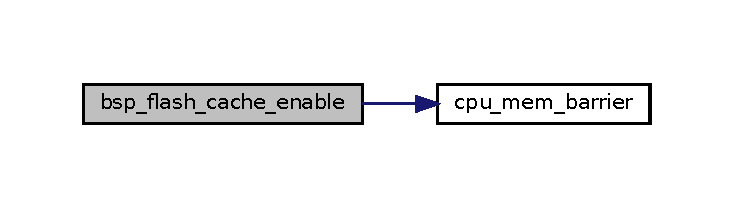
\includegraphics[width=350pt]{bsp__flash_8h_a28b133b49a8b54580ef07cc2b02b6a2d_cgraph}
\end{center}
\end{figure}
\mbox{\Hypertarget{bsp__flash_8h_a2f8e8bffdc14c9ea45296defed4606a6}\label{bsp__flash_8h_a2f8e8bffdc14c9ea45296defed4606a6}} 
\index{bsp\+\_\+flash.\+h@{bsp\+\_\+flash.\+h}!bsp\+\_\+flash\+\_\+prefetch\+\_\+enable@{bsp\+\_\+flash\+\_\+prefetch\+\_\+enable}}
\index{bsp\+\_\+flash\+\_\+prefetch\+\_\+enable@{bsp\+\_\+flash\+\_\+prefetch\+\_\+enable}!bsp\+\_\+flash.\+h@{bsp\+\_\+flash.\+h}}
\subsubsection{\texorpdfstring{bsp\+\_\+flash\+\_\+prefetch\+\_\+enable()}{bsp\_flash\_prefetch\_enable()}}
{\footnotesize\ttfamily void bsp\+\_\+flash\+\_\+prefetch\+\_\+enable (\begin{DoxyParamCaption}\item[{void}]{ }\end{DoxyParamCaption})}



Enables flash prefetech unit. 

­ $\ast$

Enables flash prefetech unit. 

Definition at line 42 of file bsp\+\_\+flash.\+c.


\begin{DoxyCode}
43 \{
44     *\hyperlink{bsp__flash_8h_a177b682ed269b91b61bf46005fca9620}{FLASH\_ACR\_REGISTER} = *\hyperlink{bsp__flash_8h_a177b682ed269b91b61bf46005fca9620}{FLASH\_ACR\_REGISTER}  |  
      \hyperlink{bsp__flash_8h_a479a3f068bb372bdf3bfc5b37846378a}{FLASH\_ACR\_PREFETCH\_EN};
45     \hyperlink{cpu__api_8h_a386c6bcf8612ed54728c6157bb83036e}{cpu\_mem\_barrier}();
46 \}
\end{DoxyCode}
Here is the call graph for this function\+:\nopagebreak
\begin{figure}[H]
\begin{center}
\leavevmode
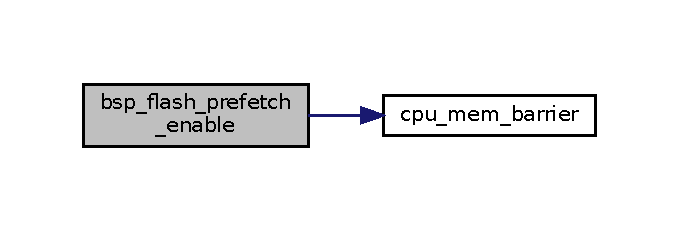
\includegraphics[width=326pt]{bsp__flash_8h_a2f8e8bffdc14c9ea45296defed4606a6_cgraph}
\end{center}
\end{figure}
\mbox{\Hypertarget{bsp__flash_8h_a51f3c79743adab8e26ca7a5c6b33c55b}\label{bsp__flash_8h_a51f3c79743adab8e26ca7a5c6b33c55b}} 
\index{bsp\+\_\+flash.\+h@{bsp\+\_\+flash.\+h}!bsp\+\_\+flash\+\_\+set\+\_\+latency@{bsp\+\_\+flash\+\_\+set\+\_\+latency}}
\index{bsp\+\_\+flash\+\_\+set\+\_\+latency@{bsp\+\_\+flash\+\_\+set\+\_\+latency}!bsp\+\_\+flash.\+h@{bsp\+\_\+flash.\+h}}
\subsubsection{\texorpdfstring{bsp\+\_\+flash\+\_\+set\+\_\+latency()}{bsp\_flash\_set\_latency()}}
{\footnotesize\ttfamily \hyperlink{error__types_8h_acf146bc98f60f47c79d782f7523e339c}{E\+R\+R\+O\+R\+\_\+\+C\+O\+D\+E\+\_\+E} bsp\+\_\+flash\+\_\+set\+\_\+latency (\begin{DoxyParamCaption}\item[{const \hyperlink{bsp__flash_8h_ab4bdf422e30b864e1ff48788fbde702d}{F\+L\+A\+S\+H\+\_\+\+L\+A\+T\+E\+N\+C\+Y\+\_\+\+W\+S\+\_\+E}}]{latency }\end{DoxyParamCaption})}



Sets the flash latency. 

­ $\ast$

Sets the flash latency based on the latency given as parameter.


\begin{DoxyParams}[1]{Parameters}
\mbox{\tt in}  & {\em latency} & The latency to set.\\
\hline
\end{DoxyParams}
\begin{DoxyReturn}{Returns}
N\+O\+\_\+\+E\+R\+R\+OR is returned in case of success. Otherwise an error code is returned. Please refer to the list of the standard error codes. 
\end{DoxyReturn}


Definition at line 48 of file bsp\+\_\+flash.\+c.


\begin{DoxyCode}
49 \{
50     \textcolor{comment}{/* Sets the flash latency value, we don't apply mask verification because 
}
51 \textcolor{comment}{     * the FLASH\_LATENCY\_WS\_E enumeration should already contain the right 
}
52 \textcolor{comment}{     * values.
}
53 \textcolor{comment}{     */}
54     *\hyperlink{bsp__flash_8h_a177b682ed269b91b61bf46005fca9620}{FLASH\_ACR\_REGISTER} = (*\hyperlink{bsp__flash_8h_a177b682ed269b91b61bf46005fca9620}{FLASH\_ACR\_REGISTER} & ~
      \hyperlink{bsp__flash_8h_a325fd0108f2a85889c495a9f08409216}{FLASH\_ACR\_LATENCY\_MASK}) | 
55                           latency;
56 
57     \textcolor{comment}{/* Delay to ensure bit update */}
58     \textcolor{keywordflow}{while}((*\hyperlink{bsp__flash_8h_a177b682ed269b91b61bf46005fca9620}{FLASH\_ACR\_REGISTER} & \hyperlink{bsp__flash_8h_a325fd0108f2a85889c495a9f08409216}{FLASH\_ACR\_LATENCY\_MASK}) != latency
      );
59 
60 \textcolor{preprocessor}{#if KERNEL\_LOG\_LEVEL >= INFO\_LOG\_LEVEL
}
61     KERNEL\_LOG\_INFO(\textcolor{stringliteral}{"Flash lantency changed"}, 
62                     latency, 
63                     \textcolor{keyword}{sizeof}(latency), 
64                     \hyperlink{error__types_8h_a4db9ee29f2ff83c71567c12f6bfbf28cabf350750d0d4fabd8954c0f1e9bbae94}{NO\_ERROR});
65 \textcolor{preprocessor}{#endif
}
66 
67     \textcolor{keywordflow}{return} \hyperlink{error__types_8h_a4db9ee29f2ff83c71567c12f6bfbf28cabf350750d0d4fabd8954c0f1e9bbae94}{NO\_ERROR};
68 \}
\end{DoxyCode}
Here is the caller graph for this function\+:\nopagebreak
\begin{figure}[H]
\begin{center}
\leavevmode
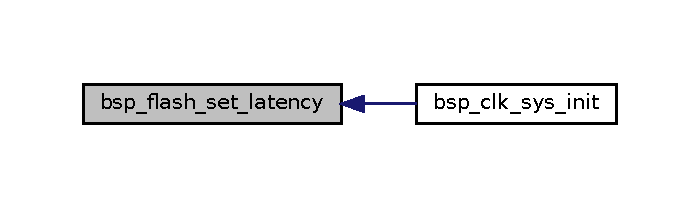
\includegraphics[width=336pt]{bsp__flash_8h_a51f3c79743adab8e26ca7a5c6b33c55b_icgraph}
\end{center}
\end{figure}

\hypertarget{bsp__gpio_8h}{}\section{Kernel/\+Sources/arch/board/stm32/f401re/includes/bsp\+\_\+gpio.h File Reference}
\label{bsp__gpio_8h}\index{Kernel/\+Sources/arch/board/stm32/f401re/includes/bsp\+\_\+gpio.\+h@{Kernel/\+Sources/arch/board/stm32/f401re/includes/bsp\+\_\+gpio.\+h}}
{\ttfamily \#include \char`\"{}error\+\_\+types.\+h\char`\"{}}\newline
{\ttfamily \#include \char`\"{}stdint.\+h\char`\"{}}\newline
Include dependency graph for bsp\+\_\+gpio.\+h\+:\nopagebreak
\begin{figure}[H]
\begin{center}
\leavevmode
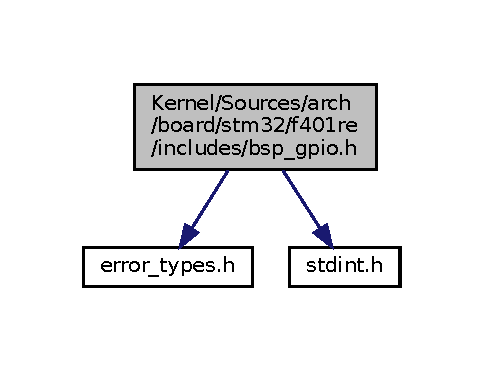
\includegraphics[width=232pt]{bsp__gpio_8h__incl}
\end{center}
\end{figure}
This graph shows which files directly or indirectly include this file\+:\nopagebreak
\begin{figure}[H]
\begin{center}
\leavevmode
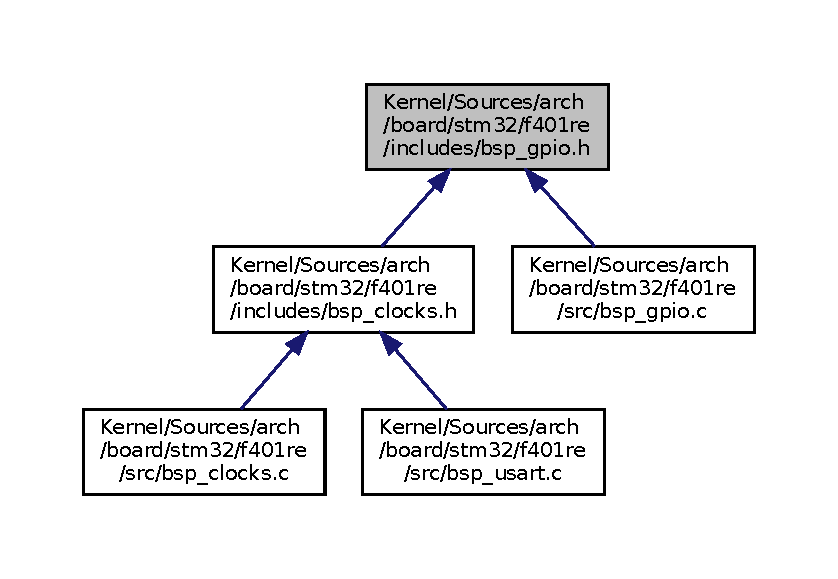
\includegraphics[width=350pt]{bsp__gpio_8h__dep__incl}
\end{center}
\end{figure}
\subsection*{Data Structures}
\begin{DoxyCompactItemize}
\item 
struct \hyperlink{struct_g_p_i_o___s_e_t_t_i_n_g_s}{G\+P\+I\+O\+\_\+\+S\+E\+T\+T\+I\+N\+GS}
\begin{DoxyCompactList}\small\item\em G\+P\+IO settings structure. Stores the G\+P\+IO settings for a given G\+P\+IO bank. \end{DoxyCompactList}\end{DoxyCompactItemize}
\subsection*{Macros}
\begin{DoxyCompactItemize}
\item 
\#define \hyperlink{bsp__gpio_8h_a72db53eb21962c0c32457008d0e0b3bf}{G\+P\+I\+O\+\_\+\+X\+\_\+\+B\+A\+S\+E\+\_\+\+A\+D\+D\+R\+E\+SS}~0x40020000
\begin{DoxyCompactList}\small\item\em G\+P\+IO registers base address. \end{DoxyCompactList}\item 
\#define \hyperlink{bsp__gpio_8h_abd2bf74240b288f8d42e6e6aa157ba52}{G\+P\+I\+O\+\_\+\+M\+O\+D\+E\+R\+\_\+\+O\+F\+F\+S\+ET}~0x00
\begin{DoxyCompactList}\small\item\em G\+P\+IO mode register offset. \end{DoxyCompactList}\item 
\#define \hyperlink{bsp__gpio_8h_a424a9ba00d1b8767830a4ba2876b81b7}{G\+P\+I\+O\+\_\+\+O\+T\+Y\+P\+E\+R\+\_\+\+O\+F\+F\+S\+ET}~0x04
\begin{DoxyCompactList}\small\item\em G\+P\+IO output type register offset. \end{DoxyCompactList}\item 
\#define \hyperlink{bsp__gpio_8h_ab361ffd58b67dc9ba2bc1d3818fd099a}{G\+P\+I\+O\+\_\+\+O\+S\+P\+E\+E\+D\+R\+\_\+\+O\+F\+F\+S\+ET}~0x08
\begin{DoxyCompactList}\small\item\em G\+P\+IO output speed register offset. \end{DoxyCompactList}\item 
\#define \hyperlink{bsp__gpio_8h_a4f90e03c8f7a5a858796d314a766c36e}{G\+P\+I\+O\+\_\+\+P\+U\+D\+R\+\_\+\+O\+F\+F\+S\+ET}~0x0C
\begin{DoxyCompactList}\small\item\em G\+P\+IO pull type registers offset. \end{DoxyCompactList}\item 
\#define \hyperlink{bsp__gpio_8h_a2a111ee9e5845dcba61cf1d7fe0eb43f}{G\+P\+I\+O\+\_\+\+A\+F\+R\+L\+\_\+\+O\+F\+F\+S\+ET}~0x20
\begin{DoxyCompactList}\small\item\em G\+P\+IO alternate function low registers offset. \end{DoxyCompactList}\item 
\#define \hyperlink{bsp__gpio_8h_afdfc1903c8131e8c47c81bc89401f12e}{G\+P\+I\+O\+\_\+\+A\+F\+R\+H\+\_\+\+O\+F\+F\+S\+ET}~0x24
\begin{DoxyCompactList}\small\item\em G\+P\+IO alternate function high registers offset. \end{DoxyCompactList}\item 
\#define \hyperlink{bsp__gpio_8h_af40bec3146810028a84b628d37d3b391}{G\+P\+I\+O\+\_\+\+M\+O\+D\+E\+\_\+\+I\+N\+P\+UT}~0x00
\begin{DoxyCompactList}\small\item\em G\+P\+IO mode\+: input IO. \end{DoxyCompactList}\item 
\#define \hyperlink{bsp__gpio_8h_aca6eb0cd4dbe7402497829badacfa6df}{G\+P\+I\+O\+\_\+\+M\+O\+D\+E\+\_\+\+O\+U\+T\+P\+UT}~0x01
\begin{DoxyCompactList}\small\item\em G\+P\+IO mode\+: output IO. \end{DoxyCompactList}\item 
\#define \hyperlink{bsp__gpio_8h_ae0c591139910f3313c998fdcf74a2b77}{G\+P\+I\+O\+\_\+\+M\+O\+D\+E\+\_\+\+A\+L\+T\+F\+UN}~0x02
\begin{DoxyCompactList}\small\item\em G\+P\+IO mode\+: alternate function IO. \end{DoxyCompactList}\item 
\#define \hyperlink{bsp__gpio_8h_a7a04f9ab65ad572ad20791a35009220c}{G\+P\+I\+O\+\_\+\+M\+O\+D\+E\+\_\+\+A\+N\+A\+L\+OG}~0x03
\begin{DoxyCompactList}\small\item\em G\+P\+IO mode\+: analog. \end{DoxyCompactList}\item 
\#define \hyperlink{bsp__gpio_8h_af9c9aabc72e4bda42794979584908a8c}{G\+P\+I\+O\+\_\+\+T\+Y\+P\+E\+\_\+\+P\+U\+S\+H\+P\+U\+LL}~0x00
\begin{DoxyCompactList}\small\item\em G\+P\+IO push/pull mode\+: push/pull. \end{DoxyCompactList}\item 
\#define \hyperlink{bsp__gpio_8h_a53ffd10a8d79d5fc15da1c29d97edb0d}{G\+P\+I\+O\+\_\+\+T\+Y\+P\+E\+\_\+\+O\+P\+E\+N\+D\+R\+A\+IN}~0x04
\begin{DoxyCompactList}\small\item\em G\+P\+IO push/pull mode\+: open drain. \end{DoxyCompactList}\item 
\#define \hyperlink{bsp__gpio_8h_a668f96c075364ffd349cc33eb75318a0}{G\+P\+I\+O\+\_\+\+S\+P\+E\+E\+D\+\_\+\+S\+L\+OW}~0x00
\begin{DoxyCompactList}\small\item\em G\+P\+IO output speed\+: slow. \end{DoxyCompactList}\item 
\#define \hyperlink{bsp__gpio_8h_a44a0eb2335a21858efbbb1557ce8d5e5}{G\+P\+I\+O\+\_\+\+S\+P\+E\+E\+D\+\_\+\+M\+E\+D\+I\+UM}~0x01
\begin{DoxyCompactList}\small\item\em G\+P\+IO output speed\+: medium. \end{DoxyCompactList}\item 
\#define \hyperlink{bsp__gpio_8h_ad693110177bf2e34c5431555c6977e8c}{G\+P\+I\+O\+\_\+\+S\+P\+E\+E\+D\+\_\+\+H\+I\+GH}~0x02
\begin{DoxyCompactList}\small\item\em G\+P\+IO output speed\+: high. \end{DoxyCompactList}\item 
\#define \hyperlink{bsp__gpio_8h_ae11603e44b5bb26398c583a2410cafd5}{G\+P\+I\+O\+\_\+\+S\+P\+E\+E\+D\+\_\+\+V\+E\+R\+Y\+\_\+\+H\+I\+GH}~0x03
\begin{DoxyCompactList}\small\item\em G\+P\+IO output speed\+: very high. \end{DoxyCompactList}\item 
\#define \hyperlink{bsp__gpio_8h_ad53ebddfcc3973120b1c0271423f131e}{G\+P\+I\+O\+\_\+\+P\+U\+P\+D\+\_\+\+N\+O\+NE}~0x00
\begin{DoxyCompactList}\small\item\em G\+P\+IO pull mode\+: none. \end{DoxyCompactList}\item 
\#define \hyperlink{bsp__gpio_8h_a23c4444d94360702b7c7f342eb696f22}{G\+P\+I\+O\+\_\+\+P\+U\+P\+D\+\_\+\+PU}~0x08
\begin{DoxyCompactList}\small\item\em G\+P\+IO pull mode\+: up. \end{DoxyCompactList}\item 
\#define \hyperlink{bsp__gpio_8h_aa461175664d6ec906f90dbfb514c50bb}{G\+P\+I\+O\+\_\+\+P\+U\+P\+D\+\_\+\+PD}~0x10
\begin{DoxyCompactList}\small\item\em G\+P\+IO pull mode\+: down. \end{DoxyCompactList}\item 
\#define \hyperlink{bsp__gpio_8h_a6da557f60e6eb28d68f645e4674daa55}{G\+P\+I\+O\+\_\+\+A\+L\+F\+U\+N\+C\+\_\+0}~0
\begin{DoxyCompactList}\small\item\em G\+P\+IO alternate function 0. \end{DoxyCompactList}\item 
\#define \hyperlink{bsp__gpio_8h_aa5169353a4da342942cc766a33da3275}{G\+P\+I\+O\+\_\+\+A\+L\+F\+U\+N\+C\+\_\+1}~1
\begin{DoxyCompactList}\small\item\em G\+P\+IO alternate function 1. \end{DoxyCompactList}\item 
\#define \hyperlink{bsp__gpio_8h_a96dc1e5393b5429f05df723b2f1376ef}{G\+P\+I\+O\+\_\+\+A\+L\+F\+U\+N\+C\+\_\+2}~2
\begin{DoxyCompactList}\small\item\em G\+P\+IO alternate function 2. \end{DoxyCompactList}\item 
\#define \hyperlink{bsp__gpio_8h_a7dbdcb25f5b65647980a866ab01fee63}{G\+P\+I\+O\+\_\+\+A\+L\+F\+U\+N\+C\+\_\+3}~3
\begin{DoxyCompactList}\small\item\em G\+P\+IO alternate function 3. \end{DoxyCompactList}\item 
\#define \hyperlink{bsp__gpio_8h_ae3f12f814bf1644bf2035e176fb30b9f}{G\+P\+I\+O\+\_\+\+A\+L\+F\+U\+N\+C\+\_\+4}~4
\begin{DoxyCompactList}\small\item\em G\+P\+IO alternate function 4. \end{DoxyCompactList}\item 
\#define \hyperlink{bsp__gpio_8h_a0e16e8fcc5eb4f9cb65dd66a70064376}{G\+P\+I\+O\+\_\+\+A\+L\+F\+U\+N\+C\+\_\+5}~5
\begin{DoxyCompactList}\small\item\em G\+P\+IO alternate function 5. \end{DoxyCompactList}\item 
\#define \hyperlink{bsp__gpio_8h_a52b37a62c80b9559c8aa265756fd8da0}{G\+P\+I\+O\+\_\+\+A\+L\+F\+U\+N\+C\+\_\+6}~6
\begin{DoxyCompactList}\small\item\em G\+P\+IO alternate function 6. \end{DoxyCompactList}\item 
\#define \hyperlink{bsp__gpio_8h_a6af3869309b2bfedca84f57a7772ee4d}{G\+P\+I\+O\+\_\+\+A\+L\+F\+U\+N\+C\+\_\+7}~7
\begin{DoxyCompactList}\small\item\em G\+P\+IO alternate function 7. \end{DoxyCompactList}\item 
\#define \hyperlink{bsp__gpio_8h_aad7b1f8e5f7070b61504f8015fbb2d65}{G\+P\+I\+O\+\_\+\+A\+L\+F\+U\+N\+C\+\_\+8}~8
\begin{DoxyCompactList}\small\item\em G\+P\+IO alternate function 8. \end{DoxyCompactList}\item 
\#define \hyperlink{bsp__gpio_8h_aa86bc8490805d4ada49b8f4e724ce3cc}{G\+P\+I\+O\+\_\+\+A\+L\+F\+U\+N\+C\+\_\+9}~9
\begin{DoxyCompactList}\small\item\em G\+P\+IO alternate function 9. \end{DoxyCompactList}\item 
\#define \hyperlink{bsp__gpio_8h_a763cb29df958df797cde84bf30e20f62}{G\+P\+I\+O\+\_\+\+A\+L\+F\+U\+N\+C\+\_\+10}~10
\begin{DoxyCompactList}\small\item\em G\+P\+IO alternate function 10. \end{DoxyCompactList}\item 
\#define \hyperlink{bsp__gpio_8h_a47dcf762b05b4a739220f07703da47c6}{G\+P\+I\+O\+\_\+\+A\+L\+F\+U\+N\+C\+\_\+11}~11
\begin{DoxyCompactList}\small\item\em G\+P\+IO alternate function 11. \end{DoxyCompactList}\item 
\#define \hyperlink{bsp__gpio_8h_aa97cd166e0cd212a21307eb6d6d7b2db}{G\+P\+I\+O\+\_\+\+A\+L\+F\+U\+N\+C\+\_\+12}~12
\begin{DoxyCompactList}\small\item\em G\+P\+IO alternate function 12. \end{DoxyCompactList}\item 
\#define \hyperlink{bsp__gpio_8h_a7b2024cb0207dc45eade4dbaef785348}{G\+P\+I\+O\+\_\+\+A\+L\+F\+U\+N\+C\+\_\+13}~13
\begin{DoxyCompactList}\small\item\em G\+P\+IO alternate function 13. \end{DoxyCompactList}\item 
\#define \hyperlink{bsp__gpio_8h_a0ff312456e2f35f4bc1d40ae68546cd4}{G\+P\+I\+O\+\_\+\+A\+L\+F\+U\+N\+C\+\_\+14}~14
\begin{DoxyCompactList}\small\item\em G\+P\+IO alternate function 14. \end{DoxyCompactList}\item 
\#define \hyperlink{bsp__gpio_8h_ad08e321e0fe351c401c3c698bba92fd7}{G\+P\+I\+O\+\_\+\+A\+L\+F\+U\+N\+C\+\_\+15}~15
\begin{DoxyCompactList}\small\item\em G\+P\+IO alternate function 15. \end{DoxyCompactList}\item 
\#define \hyperlink{bsp__gpio_8h_a60078f74d184e10418a0e1d074d6dd43}{G\+P\+I\+O\+\_\+\+M\+O\+D\+E\+\_\+\+M\+A\+SK}~0x3
\begin{DoxyCompactList}\small\item\em G\+P\+IO settings mode field mask. \end{DoxyCompactList}\item 
\#define \hyperlink{bsp__gpio_8h_aa2a5bbbcb74757aecf837db663892f63}{G\+P\+I\+O\+\_\+\+M\+O\+D\+E\+\_\+\+O\+F\+F\+S\+ET}~0
\begin{DoxyCompactList}\small\item\em G\+P\+IO settings mode field offset. \end{DoxyCompactList}\item 
\#define \hyperlink{bsp__gpio_8h_ad67ab80c9691656f1648a34d67d5f484}{G\+P\+I\+O\+\_\+\+T\+Y\+P\+E\+\_\+\+M\+A\+SK}~0x04
\begin{DoxyCompactList}\small\item\em G\+P\+IO settings type field mask. \end{DoxyCompactList}\item 
\#define \hyperlink{bsp__gpio_8h_a304f3d97adc3dc07cd5dd8187ea1aeba}{G\+P\+I\+O\+\_\+\+T\+Y\+P\+E\+\_\+\+O\+F\+F\+S\+ET}~2
\begin{DoxyCompactList}\small\item\em G\+P\+IO settings type field offset. \end{DoxyCompactList}\item 
\#define \hyperlink{bsp__gpio_8h_a8ca9d068fb34ae1e9095f0f7a69e6819}{G\+P\+I\+O\+\_\+\+P\+U\+P\+D\+\_\+\+M\+A\+SK}~0x18
\begin{DoxyCompactList}\small\item\em G\+P\+IO pull type field mask. \end{DoxyCompactList}\item 
\#define \hyperlink{bsp__gpio_8h_a738b243ba6580613802758433b10a639}{G\+P\+I\+O\+\_\+\+P\+U\+P\+D\+\_\+\+O\+F\+F\+S\+ET}~3
\begin{DoxyCompactList}\small\item\em G\+P\+IO pull type field offset. \end{DoxyCompactList}\item 
\#define \hyperlink{bsp__gpio_8h_a226e7ff497e286c3391041c1dc2f2bc2}{G\+P\+I\+O\+\_\+\+P\+I\+N\+\_\+\+C\+O\+U\+NT}~15
\begin{DoxyCompactList}\small\item\em Maximum number of pins in one G\+P\+IO bank. \end{DoxyCompactList}\item 
\#define \hyperlink{bsp__gpio_8h_a176efbf43a259b7bb0a85a47401505be}{G\+P\+I\+O\+\_\+\+P\+I\+N\+\_\+0}~0x0001
\begin{DoxyCompactList}\small\item\em G\+P\+IO bitfield\+: G\+P\+IO 0. \end{DoxyCompactList}\item 
\#define \hyperlink{bsp__gpio_8h_a6c35af4e75c3cb57bb650feaa7a136b5}{G\+P\+I\+O\+\_\+\+P\+I\+N\+\_\+1}~0x0002
\begin{DoxyCompactList}\small\item\em G\+P\+IO bitfield\+: G\+P\+IO 1. \end{DoxyCompactList}\item 
\#define \hyperlink{bsp__gpio_8h_a6eee38b797a7268f04357dfa2759efd2}{G\+P\+I\+O\+\_\+\+P\+I\+N\+\_\+2}~0x0004
\begin{DoxyCompactList}\small\item\em G\+P\+IO bitfield\+: G\+P\+IO 2. \end{DoxyCompactList}\item 
\#define \hyperlink{bsp__gpio_8h_adcaf899c018a0dde572b5af783565c62}{G\+P\+I\+O\+\_\+\+P\+I\+N\+\_\+3}~0x0008
\begin{DoxyCompactList}\small\item\em G\+P\+IO bitfield\+: G\+P\+IO 3. \end{DoxyCompactList}\item 
\#define \hyperlink{bsp__gpio_8h_ab3871e35868deecd260e586ad70d4b83}{G\+P\+I\+O\+\_\+\+P\+I\+N\+\_\+4}~0x0010
\begin{DoxyCompactList}\small\item\em G\+P\+IO bitfield\+: G\+P\+IO 4. \end{DoxyCompactList}\item 
\#define \hyperlink{bsp__gpio_8h_a01cc9ed93f6fd12fd3403362779aaa18}{G\+P\+I\+O\+\_\+\+P\+I\+N\+\_\+5}~0x0020
\begin{DoxyCompactList}\small\item\em G\+P\+IO bitfield\+: G\+P\+IO 5. \end{DoxyCompactList}\item 
\#define \hyperlink{bsp__gpio_8h_a9089f18f20ec88ee38ce6f27389e6d7e}{G\+P\+I\+O\+\_\+\+P\+I\+N\+\_\+6}~0x0040
\begin{DoxyCompactList}\small\item\em G\+P\+IO bitfield\+: G\+P\+IO 6. \end{DoxyCompactList}\item 
\#define \hyperlink{bsp__gpio_8h_a482cb86c2f036e630661a41e8986bcfe}{G\+P\+I\+O\+\_\+\+P\+I\+N\+\_\+7}~0x0080
\begin{DoxyCompactList}\small\item\em G\+P\+IO bitfield\+: G\+P\+IO 7. \end{DoxyCompactList}\item 
\#define \hyperlink{bsp__gpio_8h_af5eb6a42a4428e236bd4fd08ade71e7a}{G\+P\+I\+O\+\_\+\+P\+I\+N\+\_\+8}~0x0100
\begin{DoxyCompactList}\small\item\em G\+P\+IO bitfield\+: G\+P\+IO 8. \end{DoxyCompactList}\item 
\#define \hyperlink{bsp__gpio_8h_a4c503cb4a0dc0d18261080051d9c2daf}{G\+P\+I\+O\+\_\+\+P\+I\+N\+\_\+9}~0x0200
\begin{DoxyCompactList}\small\item\em G\+P\+IO bitfield\+: G\+P\+IO 9. \end{DoxyCompactList}\item 
\#define \hyperlink{bsp__gpio_8h_ac102c0123cb8bcadc5b590cd940b9e20}{G\+P\+I\+O\+\_\+\+P\+I\+N\+\_\+10}~0x0400
\begin{DoxyCompactList}\small\item\em G\+P\+IO bitfield\+: G\+P\+IO 10. \end{DoxyCompactList}\item 
\#define \hyperlink{bsp__gpio_8h_a79f6797ea82c1fb25cd6c0e14e44d312}{G\+P\+I\+O\+\_\+\+P\+I\+N\+\_\+11}~0x0800
\begin{DoxyCompactList}\small\item\em G\+P\+IO bitfield\+: G\+P\+IO 11. \end{DoxyCompactList}\item 
\#define \hyperlink{bsp__gpio_8h_a95f9ce5911fa8b209defb969db93ced3}{G\+P\+I\+O\+\_\+\+P\+I\+N\+\_\+12}~0x1000
\begin{DoxyCompactList}\small\item\em G\+P\+IO bitfield\+: G\+P\+IO 12. \end{DoxyCompactList}\item 
\#define \hyperlink{bsp__gpio_8h_a173023dced8f9692ade0f1176558ef70}{G\+P\+I\+O\+\_\+\+P\+I\+N\+\_\+13}~0x2000
\begin{DoxyCompactList}\small\item\em G\+P\+IO bitfield\+: G\+P\+IO 13. \end{DoxyCompactList}\item 
\#define \hyperlink{bsp__gpio_8h_a315b4dc1a0c1f9021b3d3a8fe9ccc0c3}{G\+P\+I\+O\+\_\+\+P\+I\+N\+\_\+14}~0x4000
\begin{DoxyCompactList}\small\item\em G\+P\+IO bitfield\+: G\+P\+IO 14. \end{DoxyCompactList}\item 
\#define \hyperlink{bsp__gpio_8h_a77be5756e80bcdf18e1aa39b35d1d640}{G\+P\+I\+O\+\_\+\+P\+I\+N\+\_\+15}~0x8000
\begin{DoxyCompactList}\small\item\em G\+P\+IO bitfield\+: G\+P\+IO 15. \end{DoxyCompactList}\end{DoxyCompactItemize}
\subsection*{Typedefs}
\begin{DoxyCompactItemize}
\item 
typedef enum \hyperlink{bsp__gpio_8h_a69f521b579d2c761dd65949f2bae88f3}{G\+P\+I\+O\+\_\+\+I\+D\+E\+N\+T\+I\+F\+I\+ER} \hyperlink{bsp__gpio_8h_ab086506332275a2a873dfce02ed5a3b8}{G\+P\+I\+O\+\_\+\+I\+D\+E\+N\+T\+I\+F\+I\+E\+R\+\_\+E}
\begin{DoxyCompactList}\small\item\em Short hand for enum G\+P\+I\+O\+\_\+\+I\+D\+E\+N\+T\+I\+F\+I\+ER. \end{DoxyCompactList}\item 
typedef struct \hyperlink{struct_g_p_i_o___s_e_t_t_i_n_g_s}{G\+P\+I\+O\+\_\+\+S\+E\+T\+T\+I\+N\+GS} \hyperlink{bsp__gpio_8h_ad7cd0faab6d093c8c9c399372e147467}{G\+P\+I\+O\+\_\+\+S\+E\+T\+T\+I\+N\+G\+S\+\_\+T}
\begin{DoxyCompactList}\small\item\em Short hand for struct \hyperlink{struct_g_p_i_o___s_e_t_t_i_n_g_s}{G\+P\+I\+O\+\_\+\+S\+E\+T\+T\+I\+N\+GS}. \end{DoxyCompactList}\end{DoxyCompactItemize}
\subsection*{Enumerations}
\begin{DoxyCompactItemize}
\item 
enum \hyperlink{bsp__gpio_8h_a69f521b579d2c761dd65949f2bae88f3}{G\+P\+I\+O\+\_\+\+I\+D\+E\+N\+T\+I\+F\+I\+ER} \{ \newline
\hyperlink{bsp__gpio_8h_a69f521b579d2c761dd65949f2bae88f3a4cb73b98ec508807d984052a1598950a}{G\+P\+I\+O\+\_\+\+I\+D\+\_\+A} = 0, 
\hyperlink{bsp__gpio_8h_a69f521b579d2c761dd65949f2bae88f3a9fc59b324d277c00de32d87f8072b56a}{G\+P\+I\+O\+\_\+\+I\+D\+\_\+B} = 1, 
\hyperlink{bsp__gpio_8h_a69f521b579d2c761dd65949f2bae88f3afae76fa0a334173cbea6472ae010d0a9}{G\+P\+I\+O\+\_\+\+I\+D\+\_\+C} = 2, 
\hyperlink{bsp__gpio_8h_a69f521b579d2c761dd65949f2bae88f3ad6df84175b0fc74ef3c655082b648918}{G\+P\+I\+O\+\_\+\+I\+D\+\_\+D} = 3, 
\newline
\hyperlink{bsp__gpio_8h_a69f521b579d2c761dd65949f2bae88f3a496fabc0d5663f4956df5e9a4d275ed4}{G\+P\+I\+O\+\_\+\+I\+D\+\_\+E} = 4, 
\hyperlink{bsp__gpio_8h_a69f521b579d2c761dd65949f2bae88f3aa25ae326f6c8e013c190052d0a3c7d29}{G\+P\+I\+O\+\_\+\+I\+D\+\_\+H} = 5
 \}\begin{DoxyCompactList}\small\item\em G\+P\+IO identifier used to differenciated the G\+P\+I\+Os present on the S\+T\+M32\+F401\+RE board. \end{DoxyCompactList}
\end{DoxyCompactItemize}
\subsection*{Functions}
\begin{DoxyCompactItemize}
\item 
\hyperlink{error__types_8h_acf146bc98f60f47c79d782f7523e339c}{E\+R\+R\+O\+R\+\_\+\+C\+O\+D\+E\+\_\+E} \hyperlink{bsp__gpio_8h_ac05d93f29cf8cdcd3809298fe5df2f87}{bsp\+\_\+gpio\+\_\+init} (const \hyperlink{bsp__gpio_8h_ab086506332275a2a873dfce02ed5a3b8}{G\+P\+I\+O\+\_\+\+I\+D\+E\+N\+T\+I\+F\+I\+E\+R\+\_\+E} gpio\+\_\+id, const \hyperlink{bsp__gpio_8h_ad7cd0faab6d093c8c9c399372e147467}{G\+P\+I\+O\+\_\+\+S\+E\+T\+T\+I\+N\+G\+S\+\_\+T} $\ast$settings)
\begin{DoxyCompactList}\small\item\em Initializes a given G\+P\+IO bank. \end{DoxyCompactList}\end{DoxyCompactItemize}


\subsection{Macro Definition Documentation}
\mbox{\Hypertarget{bsp__gpio_8h_afdfc1903c8131e8c47c81bc89401f12e}\label{bsp__gpio_8h_afdfc1903c8131e8c47c81bc89401f12e}} 
\index{bsp\+\_\+gpio.\+h@{bsp\+\_\+gpio.\+h}!G\+P\+I\+O\+\_\+\+A\+F\+R\+H\+\_\+\+O\+F\+F\+S\+ET@{G\+P\+I\+O\+\_\+\+A\+F\+R\+H\+\_\+\+O\+F\+F\+S\+ET}}
\index{G\+P\+I\+O\+\_\+\+A\+F\+R\+H\+\_\+\+O\+F\+F\+S\+ET@{G\+P\+I\+O\+\_\+\+A\+F\+R\+H\+\_\+\+O\+F\+F\+S\+ET}!bsp\+\_\+gpio.\+h@{bsp\+\_\+gpio.\+h}}
\subsubsection{\texorpdfstring{G\+P\+I\+O\+\_\+\+A\+F\+R\+H\+\_\+\+O\+F\+F\+S\+ET}{GPIO\_AFRH\_OFFSET}}
{\footnotesize\ttfamily \#define G\+P\+I\+O\+\_\+\+A\+F\+R\+H\+\_\+\+O\+F\+F\+S\+ET~0x24}



G\+P\+IO alternate function high registers offset. 



Definition at line 39 of file bsp\+\_\+gpio.\+h.

\mbox{\Hypertarget{bsp__gpio_8h_a2a111ee9e5845dcba61cf1d7fe0eb43f}\label{bsp__gpio_8h_a2a111ee9e5845dcba61cf1d7fe0eb43f}} 
\index{bsp\+\_\+gpio.\+h@{bsp\+\_\+gpio.\+h}!G\+P\+I\+O\+\_\+\+A\+F\+R\+L\+\_\+\+O\+F\+F\+S\+ET@{G\+P\+I\+O\+\_\+\+A\+F\+R\+L\+\_\+\+O\+F\+F\+S\+ET}}
\index{G\+P\+I\+O\+\_\+\+A\+F\+R\+L\+\_\+\+O\+F\+F\+S\+ET@{G\+P\+I\+O\+\_\+\+A\+F\+R\+L\+\_\+\+O\+F\+F\+S\+ET}!bsp\+\_\+gpio.\+h@{bsp\+\_\+gpio.\+h}}
\subsubsection{\texorpdfstring{G\+P\+I\+O\+\_\+\+A\+F\+R\+L\+\_\+\+O\+F\+F\+S\+ET}{GPIO\_AFRL\_OFFSET}}
{\footnotesize\ttfamily \#define G\+P\+I\+O\+\_\+\+A\+F\+R\+L\+\_\+\+O\+F\+F\+S\+ET~0x20}



G\+P\+IO alternate function low registers offset. 



Definition at line 37 of file bsp\+\_\+gpio.\+h.

\mbox{\Hypertarget{bsp__gpio_8h_a6da557f60e6eb28d68f645e4674daa55}\label{bsp__gpio_8h_a6da557f60e6eb28d68f645e4674daa55}} 
\index{bsp\+\_\+gpio.\+h@{bsp\+\_\+gpio.\+h}!G\+P\+I\+O\+\_\+\+A\+L\+F\+U\+N\+C\+\_\+0@{G\+P\+I\+O\+\_\+\+A\+L\+F\+U\+N\+C\+\_\+0}}
\index{G\+P\+I\+O\+\_\+\+A\+L\+F\+U\+N\+C\+\_\+0@{G\+P\+I\+O\+\_\+\+A\+L\+F\+U\+N\+C\+\_\+0}!bsp\+\_\+gpio.\+h@{bsp\+\_\+gpio.\+h}}
\subsubsection{\texorpdfstring{G\+P\+I\+O\+\_\+\+A\+L\+F\+U\+N\+C\+\_\+0}{GPIO\_ALFUNC\_0}}
{\footnotesize\ttfamily \#define G\+P\+I\+O\+\_\+\+A\+L\+F\+U\+N\+C\+\_\+0~0}



G\+P\+IO alternate function 0. 



Definition at line 72 of file bsp\+\_\+gpio.\+h.

\mbox{\Hypertarget{bsp__gpio_8h_aa5169353a4da342942cc766a33da3275}\label{bsp__gpio_8h_aa5169353a4da342942cc766a33da3275}} 
\index{bsp\+\_\+gpio.\+h@{bsp\+\_\+gpio.\+h}!G\+P\+I\+O\+\_\+\+A\+L\+F\+U\+N\+C\+\_\+1@{G\+P\+I\+O\+\_\+\+A\+L\+F\+U\+N\+C\+\_\+1}}
\index{G\+P\+I\+O\+\_\+\+A\+L\+F\+U\+N\+C\+\_\+1@{G\+P\+I\+O\+\_\+\+A\+L\+F\+U\+N\+C\+\_\+1}!bsp\+\_\+gpio.\+h@{bsp\+\_\+gpio.\+h}}
\subsubsection{\texorpdfstring{G\+P\+I\+O\+\_\+\+A\+L\+F\+U\+N\+C\+\_\+1}{GPIO\_ALFUNC\_1}}
{\footnotesize\ttfamily \#define G\+P\+I\+O\+\_\+\+A\+L\+F\+U\+N\+C\+\_\+1~1}



G\+P\+IO alternate function 1. 



Definition at line 74 of file bsp\+\_\+gpio.\+h.

\mbox{\Hypertarget{bsp__gpio_8h_a763cb29df958df797cde84bf30e20f62}\label{bsp__gpio_8h_a763cb29df958df797cde84bf30e20f62}} 
\index{bsp\+\_\+gpio.\+h@{bsp\+\_\+gpio.\+h}!G\+P\+I\+O\+\_\+\+A\+L\+F\+U\+N\+C\+\_\+10@{G\+P\+I\+O\+\_\+\+A\+L\+F\+U\+N\+C\+\_\+10}}
\index{G\+P\+I\+O\+\_\+\+A\+L\+F\+U\+N\+C\+\_\+10@{G\+P\+I\+O\+\_\+\+A\+L\+F\+U\+N\+C\+\_\+10}!bsp\+\_\+gpio.\+h@{bsp\+\_\+gpio.\+h}}
\subsubsection{\texorpdfstring{G\+P\+I\+O\+\_\+\+A\+L\+F\+U\+N\+C\+\_\+10}{GPIO\_ALFUNC\_10}}
{\footnotesize\ttfamily \#define G\+P\+I\+O\+\_\+\+A\+L\+F\+U\+N\+C\+\_\+10~10}



G\+P\+IO alternate function 10. 



Definition at line 92 of file bsp\+\_\+gpio.\+h.

\mbox{\Hypertarget{bsp__gpio_8h_a47dcf762b05b4a739220f07703da47c6}\label{bsp__gpio_8h_a47dcf762b05b4a739220f07703da47c6}} 
\index{bsp\+\_\+gpio.\+h@{bsp\+\_\+gpio.\+h}!G\+P\+I\+O\+\_\+\+A\+L\+F\+U\+N\+C\+\_\+11@{G\+P\+I\+O\+\_\+\+A\+L\+F\+U\+N\+C\+\_\+11}}
\index{G\+P\+I\+O\+\_\+\+A\+L\+F\+U\+N\+C\+\_\+11@{G\+P\+I\+O\+\_\+\+A\+L\+F\+U\+N\+C\+\_\+11}!bsp\+\_\+gpio.\+h@{bsp\+\_\+gpio.\+h}}
\subsubsection{\texorpdfstring{G\+P\+I\+O\+\_\+\+A\+L\+F\+U\+N\+C\+\_\+11}{GPIO\_ALFUNC\_11}}
{\footnotesize\ttfamily \#define G\+P\+I\+O\+\_\+\+A\+L\+F\+U\+N\+C\+\_\+11~11}



G\+P\+IO alternate function 11. 



Definition at line 94 of file bsp\+\_\+gpio.\+h.

\mbox{\Hypertarget{bsp__gpio_8h_aa97cd166e0cd212a21307eb6d6d7b2db}\label{bsp__gpio_8h_aa97cd166e0cd212a21307eb6d6d7b2db}} 
\index{bsp\+\_\+gpio.\+h@{bsp\+\_\+gpio.\+h}!G\+P\+I\+O\+\_\+\+A\+L\+F\+U\+N\+C\+\_\+12@{G\+P\+I\+O\+\_\+\+A\+L\+F\+U\+N\+C\+\_\+12}}
\index{G\+P\+I\+O\+\_\+\+A\+L\+F\+U\+N\+C\+\_\+12@{G\+P\+I\+O\+\_\+\+A\+L\+F\+U\+N\+C\+\_\+12}!bsp\+\_\+gpio.\+h@{bsp\+\_\+gpio.\+h}}
\subsubsection{\texorpdfstring{G\+P\+I\+O\+\_\+\+A\+L\+F\+U\+N\+C\+\_\+12}{GPIO\_ALFUNC\_12}}
{\footnotesize\ttfamily \#define G\+P\+I\+O\+\_\+\+A\+L\+F\+U\+N\+C\+\_\+12~12}



G\+P\+IO alternate function 12. 



Definition at line 96 of file bsp\+\_\+gpio.\+h.

\mbox{\Hypertarget{bsp__gpio_8h_a7b2024cb0207dc45eade4dbaef785348}\label{bsp__gpio_8h_a7b2024cb0207dc45eade4dbaef785348}} 
\index{bsp\+\_\+gpio.\+h@{bsp\+\_\+gpio.\+h}!G\+P\+I\+O\+\_\+\+A\+L\+F\+U\+N\+C\+\_\+13@{G\+P\+I\+O\+\_\+\+A\+L\+F\+U\+N\+C\+\_\+13}}
\index{G\+P\+I\+O\+\_\+\+A\+L\+F\+U\+N\+C\+\_\+13@{G\+P\+I\+O\+\_\+\+A\+L\+F\+U\+N\+C\+\_\+13}!bsp\+\_\+gpio.\+h@{bsp\+\_\+gpio.\+h}}
\subsubsection{\texorpdfstring{G\+P\+I\+O\+\_\+\+A\+L\+F\+U\+N\+C\+\_\+13}{GPIO\_ALFUNC\_13}}
{\footnotesize\ttfamily \#define G\+P\+I\+O\+\_\+\+A\+L\+F\+U\+N\+C\+\_\+13~13}



G\+P\+IO alternate function 13. 



Definition at line 98 of file bsp\+\_\+gpio.\+h.

\mbox{\Hypertarget{bsp__gpio_8h_a0ff312456e2f35f4bc1d40ae68546cd4}\label{bsp__gpio_8h_a0ff312456e2f35f4bc1d40ae68546cd4}} 
\index{bsp\+\_\+gpio.\+h@{bsp\+\_\+gpio.\+h}!G\+P\+I\+O\+\_\+\+A\+L\+F\+U\+N\+C\+\_\+14@{G\+P\+I\+O\+\_\+\+A\+L\+F\+U\+N\+C\+\_\+14}}
\index{G\+P\+I\+O\+\_\+\+A\+L\+F\+U\+N\+C\+\_\+14@{G\+P\+I\+O\+\_\+\+A\+L\+F\+U\+N\+C\+\_\+14}!bsp\+\_\+gpio.\+h@{bsp\+\_\+gpio.\+h}}
\subsubsection{\texorpdfstring{G\+P\+I\+O\+\_\+\+A\+L\+F\+U\+N\+C\+\_\+14}{GPIO\_ALFUNC\_14}}
{\footnotesize\ttfamily \#define G\+P\+I\+O\+\_\+\+A\+L\+F\+U\+N\+C\+\_\+14~14}



G\+P\+IO alternate function 14. 



Definition at line 100 of file bsp\+\_\+gpio.\+h.

\mbox{\Hypertarget{bsp__gpio_8h_ad08e321e0fe351c401c3c698bba92fd7}\label{bsp__gpio_8h_ad08e321e0fe351c401c3c698bba92fd7}} 
\index{bsp\+\_\+gpio.\+h@{bsp\+\_\+gpio.\+h}!G\+P\+I\+O\+\_\+\+A\+L\+F\+U\+N\+C\+\_\+15@{G\+P\+I\+O\+\_\+\+A\+L\+F\+U\+N\+C\+\_\+15}}
\index{G\+P\+I\+O\+\_\+\+A\+L\+F\+U\+N\+C\+\_\+15@{G\+P\+I\+O\+\_\+\+A\+L\+F\+U\+N\+C\+\_\+15}!bsp\+\_\+gpio.\+h@{bsp\+\_\+gpio.\+h}}
\subsubsection{\texorpdfstring{G\+P\+I\+O\+\_\+\+A\+L\+F\+U\+N\+C\+\_\+15}{GPIO\_ALFUNC\_15}}
{\footnotesize\ttfamily \#define G\+P\+I\+O\+\_\+\+A\+L\+F\+U\+N\+C\+\_\+15~15}



G\+P\+IO alternate function 15. 



Definition at line 102 of file bsp\+\_\+gpio.\+h.

\mbox{\Hypertarget{bsp__gpio_8h_a96dc1e5393b5429f05df723b2f1376ef}\label{bsp__gpio_8h_a96dc1e5393b5429f05df723b2f1376ef}} 
\index{bsp\+\_\+gpio.\+h@{bsp\+\_\+gpio.\+h}!G\+P\+I\+O\+\_\+\+A\+L\+F\+U\+N\+C\+\_\+2@{G\+P\+I\+O\+\_\+\+A\+L\+F\+U\+N\+C\+\_\+2}}
\index{G\+P\+I\+O\+\_\+\+A\+L\+F\+U\+N\+C\+\_\+2@{G\+P\+I\+O\+\_\+\+A\+L\+F\+U\+N\+C\+\_\+2}!bsp\+\_\+gpio.\+h@{bsp\+\_\+gpio.\+h}}
\subsubsection{\texorpdfstring{G\+P\+I\+O\+\_\+\+A\+L\+F\+U\+N\+C\+\_\+2}{GPIO\_ALFUNC\_2}}
{\footnotesize\ttfamily \#define G\+P\+I\+O\+\_\+\+A\+L\+F\+U\+N\+C\+\_\+2~2}



G\+P\+IO alternate function 2. 



Definition at line 76 of file bsp\+\_\+gpio.\+h.

\mbox{\Hypertarget{bsp__gpio_8h_a7dbdcb25f5b65647980a866ab01fee63}\label{bsp__gpio_8h_a7dbdcb25f5b65647980a866ab01fee63}} 
\index{bsp\+\_\+gpio.\+h@{bsp\+\_\+gpio.\+h}!G\+P\+I\+O\+\_\+\+A\+L\+F\+U\+N\+C\+\_\+3@{G\+P\+I\+O\+\_\+\+A\+L\+F\+U\+N\+C\+\_\+3}}
\index{G\+P\+I\+O\+\_\+\+A\+L\+F\+U\+N\+C\+\_\+3@{G\+P\+I\+O\+\_\+\+A\+L\+F\+U\+N\+C\+\_\+3}!bsp\+\_\+gpio.\+h@{bsp\+\_\+gpio.\+h}}
\subsubsection{\texorpdfstring{G\+P\+I\+O\+\_\+\+A\+L\+F\+U\+N\+C\+\_\+3}{GPIO\_ALFUNC\_3}}
{\footnotesize\ttfamily \#define G\+P\+I\+O\+\_\+\+A\+L\+F\+U\+N\+C\+\_\+3~3}



G\+P\+IO alternate function 3. 



Definition at line 78 of file bsp\+\_\+gpio.\+h.

\mbox{\Hypertarget{bsp__gpio_8h_ae3f12f814bf1644bf2035e176fb30b9f}\label{bsp__gpio_8h_ae3f12f814bf1644bf2035e176fb30b9f}} 
\index{bsp\+\_\+gpio.\+h@{bsp\+\_\+gpio.\+h}!G\+P\+I\+O\+\_\+\+A\+L\+F\+U\+N\+C\+\_\+4@{G\+P\+I\+O\+\_\+\+A\+L\+F\+U\+N\+C\+\_\+4}}
\index{G\+P\+I\+O\+\_\+\+A\+L\+F\+U\+N\+C\+\_\+4@{G\+P\+I\+O\+\_\+\+A\+L\+F\+U\+N\+C\+\_\+4}!bsp\+\_\+gpio.\+h@{bsp\+\_\+gpio.\+h}}
\subsubsection{\texorpdfstring{G\+P\+I\+O\+\_\+\+A\+L\+F\+U\+N\+C\+\_\+4}{GPIO\_ALFUNC\_4}}
{\footnotesize\ttfamily \#define G\+P\+I\+O\+\_\+\+A\+L\+F\+U\+N\+C\+\_\+4~4}



G\+P\+IO alternate function 4. 



Definition at line 80 of file bsp\+\_\+gpio.\+h.

\mbox{\Hypertarget{bsp__gpio_8h_a0e16e8fcc5eb4f9cb65dd66a70064376}\label{bsp__gpio_8h_a0e16e8fcc5eb4f9cb65dd66a70064376}} 
\index{bsp\+\_\+gpio.\+h@{bsp\+\_\+gpio.\+h}!G\+P\+I\+O\+\_\+\+A\+L\+F\+U\+N\+C\+\_\+5@{G\+P\+I\+O\+\_\+\+A\+L\+F\+U\+N\+C\+\_\+5}}
\index{G\+P\+I\+O\+\_\+\+A\+L\+F\+U\+N\+C\+\_\+5@{G\+P\+I\+O\+\_\+\+A\+L\+F\+U\+N\+C\+\_\+5}!bsp\+\_\+gpio.\+h@{bsp\+\_\+gpio.\+h}}
\subsubsection{\texorpdfstring{G\+P\+I\+O\+\_\+\+A\+L\+F\+U\+N\+C\+\_\+5}{GPIO\_ALFUNC\_5}}
{\footnotesize\ttfamily \#define G\+P\+I\+O\+\_\+\+A\+L\+F\+U\+N\+C\+\_\+5~5}



G\+P\+IO alternate function 5. 



Definition at line 82 of file bsp\+\_\+gpio.\+h.

\mbox{\Hypertarget{bsp__gpio_8h_a52b37a62c80b9559c8aa265756fd8da0}\label{bsp__gpio_8h_a52b37a62c80b9559c8aa265756fd8da0}} 
\index{bsp\+\_\+gpio.\+h@{bsp\+\_\+gpio.\+h}!G\+P\+I\+O\+\_\+\+A\+L\+F\+U\+N\+C\+\_\+6@{G\+P\+I\+O\+\_\+\+A\+L\+F\+U\+N\+C\+\_\+6}}
\index{G\+P\+I\+O\+\_\+\+A\+L\+F\+U\+N\+C\+\_\+6@{G\+P\+I\+O\+\_\+\+A\+L\+F\+U\+N\+C\+\_\+6}!bsp\+\_\+gpio.\+h@{bsp\+\_\+gpio.\+h}}
\subsubsection{\texorpdfstring{G\+P\+I\+O\+\_\+\+A\+L\+F\+U\+N\+C\+\_\+6}{GPIO\_ALFUNC\_6}}
{\footnotesize\ttfamily \#define G\+P\+I\+O\+\_\+\+A\+L\+F\+U\+N\+C\+\_\+6~6}



G\+P\+IO alternate function 6. 



Definition at line 84 of file bsp\+\_\+gpio.\+h.

\mbox{\Hypertarget{bsp__gpio_8h_a6af3869309b2bfedca84f57a7772ee4d}\label{bsp__gpio_8h_a6af3869309b2bfedca84f57a7772ee4d}} 
\index{bsp\+\_\+gpio.\+h@{bsp\+\_\+gpio.\+h}!G\+P\+I\+O\+\_\+\+A\+L\+F\+U\+N\+C\+\_\+7@{G\+P\+I\+O\+\_\+\+A\+L\+F\+U\+N\+C\+\_\+7}}
\index{G\+P\+I\+O\+\_\+\+A\+L\+F\+U\+N\+C\+\_\+7@{G\+P\+I\+O\+\_\+\+A\+L\+F\+U\+N\+C\+\_\+7}!bsp\+\_\+gpio.\+h@{bsp\+\_\+gpio.\+h}}
\subsubsection{\texorpdfstring{G\+P\+I\+O\+\_\+\+A\+L\+F\+U\+N\+C\+\_\+7}{GPIO\_ALFUNC\_7}}
{\footnotesize\ttfamily \#define G\+P\+I\+O\+\_\+\+A\+L\+F\+U\+N\+C\+\_\+7~7}



G\+P\+IO alternate function 7. 



Definition at line 86 of file bsp\+\_\+gpio.\+h.

\mbox{\Hypertarget{bsp__gpio_8h_aad7b1f8e5f7070b61504f8015fbb2d65}\label{bsp__gpio_8h_aad7b1f8e5f7070b61504f8015fbb2d65}} 
\index{bsp\+\_\+gpio.\+h@{bsp\+\_\+gpio.\+h}!G\+P\+I\+O\+\_\+\+A\+L\+F\+U\+N\+C\+\_\+8@{G\+P\+I\+O\+\_\+\+A\+L\+F\+U\+N\+C\+\_\+8}}
\index{G\+P\+I\+O\+\_\+\+A\+L\+F\+U\+N\+C\+\_\+8@{G\+P\+I\+O\+\_\+\+A\+L\+F\+U\+N\+C\+\_\+8}!bsp\+\_\+gpio.\+h@{bsp\+\_\+gpio.\+h}}
\subsubsection{\texorpdfstring{G\+P\+I\+O\+\_\+\+A\+L\+F\+U\+N\+C\+\_\+8}{GPIO\_ALFUNC\_8}}
{\footnotesize\ttfamily \#define G\+P\+I\+O\+\_\+\+A\+L\+F\+U\+N\+C\+\_\+8~8}



G\+P\+IO alternate function 8. 



Definition at line 88 of file bsp\+\_\+gpio.\+h.

\mbox{\Hypertarget{bsp__gpio_8h_aa86bc8490805d4ada49b8f4e724ce3cc}\label{bsp__gpio_8h_aa86bc8490805d4ada49b8f4e724ce3cc}} 
\index{bsp\+\_\+gpio.\+h@{bsp\+\_\+gpio.\+h}!G\+P\+I\+O\+\_\+\+A\+L\+F\+U\+N\+C\+\_\+9@{G\+P\+I\+O\+\_\+\+A\+L\+F\+U\+N\+C\+\_\+9}}
\index{G\+P\+I\+O\+\_\+\+A\+L\+F\+U\+N\+C\+\_\+9@{G\+P\+I\+O\+\_\+\+A\+L\+F\+U\+N\+C\+\_\+9}!bsp\+\_\+gpio.\+h@{bsp\+\_\+gpio.\+h}}
\subsubsection{\texorpdfstring{G\+P\+I\+O\+\_\+\+A\+L\+F\+U\+N\+C\+\_\+9}{GPIO\_ALFUNC\_9}}
{\footnotesize\ttfamily \#define G\+P\+I\+O\+\_\+\+A\+L\+F\+U\+N\+C\+\_\+9~9}



G\+P\+IO alternate function 9. 



Definition at line 90 of file bsp\+\_\+gpio.\+h.

\mbox{\Hypertarget{bsp__gpio_8h_ae0c591139910f3313c998fdcf74a2b77}\label{bsp__gpio_8h_ae0c591139910f3313c998fdcf74a2b77}} 
\index{bsp\+\_\+gpio.\+h@{bsp\+\_\+gpio.\+h}!G\+P\+I\+O\+\_\+\+M\+O\+D\+E\+\_\+\+A\+L\+T\+F\+UN@{G\+P\+I\+O\+\_\+\+M\+O\+D\+E\+\_\+\+A\+L\+T\+F\+UN}}
\index{G\+P\+I\+O\+\_\+\+M\+O\+D\+E\+\_\+\+A\+L\+T\+F\+UN@{G\+P\+I\+O\+\_\+\+M\+O\+D\+E\+\_\+\+A\+L\+T\+F\+UN}!bsp\+\_\+gpio.\+h@{bsp\+\_\+gpio.\+h}}
\subsubsection{\texorpdfstring{G\+P\+I\+O\+\_\+\+M\+O\+D\+E\+\_\+\+A\+L\+T\+F\+UN}{GPIO\_MODE\_ALTFUN}}
{\footnotesize\ttfamily \#define G\+P\+I\+O\+\_\+\+M\+O\+D\+E\+\_\+\+A\+L\+T\+F\+UN~0x02}



G\+P\+IO mode\+: alternate function IO. 



Definition at line 46 of file bsp\+\_\+gpio.\+h.

\mbox{\Hypertarget{bsp__gpio_8h_a7a04f9ab65ad572ad20791a35009220c}\label{bsp__gpio_8h_a7a04f9ab65ad572ad20791a35009220c}} 
\index{bsp\+\_\+gpio.\+h@{bsp\+\_\+gpio.\+h}!G\+P\+I\+O\+\_\+\+M\+O\+D\+E\+\_\+\+A\+N\+A\+L\+OG@{G\+P\+I\+O\+\_\+\+M\+O\+D\+E\+\_\+\+A\+N\+A\+L\+OG}}
\index{G\+P\+I\+O\+\_\+\+M\+O\+D\+E\+\_\+\+A\+N\+A\+L\+OG@{G\+P\+I\+O\+\_\+\+M\+O\+D\+E\+\_\+\+A\+N\+A\+L\+OG}!bsp\+\_\+gpio.\+h@{bsp\+\_\+gpio.\+h}}
\subsubsection{\texorpdfstring{G\+P\+I\+O\+\_\+\+M\+O\+D\+E\+\_\+\+A\+N\+A\+L\+OG}{GPIO\_MODE\_ANALOG}}
{\footnotesize\ttfamily \#define G\+P\+I\+O\+\_\+\+M\+O\+D\+E\+\_\+\+A\+N\+A\+L\+OG~0x03}



G\+P\+IO mode\+: analog. 



Definition at line 48 of file bsp\+\_\+gpio.\+h.

\mbox{\Hypertarget{bsp__gpio_8h_af40bec3146810028a84b628d37d3b391}\label{bsp__gpio_8h_af40bec3146810028a84b628d37d3b391}} 
\index{bsp\+\_\+gpio.\+h@{bsp\+\_\+gpio.\+h}!G\+P\+I\+O\+\_\+\+M\+O\+D\+E\+\_\+\+I\+N\+P\+UT@{G\+P\+I\+O\+\_\+\+M\+O\+D\+E\+\_\+\+I\+N\+P\+UT}}
\index{G\+P\+I\+O\+\_\+\+M\+O\+D\+E\+\_\+\+I\+N\+P\+UT@{G\+P\+I\+O\+\_\+\+M\+O\+D\+E\+\_\+\+I\+N\+P\+UT}!bsp\+\_\+gpio.\+h@{bsp\+\_\+gpio.\+h}}
\subsubsection{\texorpdfstring{G\+P\+I\+O\+\_\+\+M\+O\+D\+E\+\_\+\+I\+N\+P\+UT}{GPIO\_MODE\_INPUT}}
{\footnotesize\ttfamily \#define G\+P\+I\+O\+\_\+\+M\+O\+D\+E\+\_\+\+I\+N\+P\+UT~0x00}



G\+P\+IO mode\+: input IO. 



Definition at line 42 of file bsp\+\_\+gpio.\+h.

\mbox{\Hypertarget{bsp__gpio_8h_a60078f74d184e10418a0e1d074d6dd43}\label{bsp__gpio_8h_a60078f74d184e10418a0e1d074d6dd43}} 
\index{bsp\+\_\+gpio.\+h@{bsp\+\_\+gpio.\+h}!G\+P\+I\+O\+\_\+\+M\+O\+D\+E\+\_\+\+M\+A\+SK@{G\+P\+I\+O\+\_\+\+M\+O\+D\+E\+\_\+\+M\+A\+SK}}
\index{G\+P\+I\+O\+\_\+\+M\+O\+D\+E\+\_\+\+M\+A\+SK@{G\+P\+I\+O\+\_\+\+M\+O\+D\+E\+\_\+\+M\+A\+SK}!bsp\+\_\+gpio.\+h@{bsp\+\_\+gpio.\+h}}
\subsubsection{\texorpdfstring{G\+P\+I\+O\+\_\+\+M\+O\+D\+E\+\_\+\+M\+A\+SK}{GPIO\_MODE\_MASK}}
{\footnotesize\ttfamily \#define G\+P\+I\+O\+\_\+\+M\+O\+D\+E\+\_\+\+M\+A\+SK~0x3}



G\+P\+IO settings mode field mask. 



Definition at line 105 of file bsp\+\_\+gpio.\+h.

\mbox{\Hypertarget{bsp__gpio_8h_aa2a5bbbcb74757aecf837db663892f63}\label{bsp__gpio_8h_aa2a5bbbcb74757aecf837db663892f63}} 
\index{bsp\+\_\+gpio.\+h@{bsp\+\_\+gpio.\+h}!G\+P\+I\+O\+\_\+\+M\+O\+D\+E\+\_\+\+O\+F\+F\+S\+ET@{G\+P\+I\+O\+\_\+\+M\+O\+D\+E\+\_\+\+O\+F\+F\+S\+ET}}
\index{G\+P\+I\+O\+\_\+\+M\+O\+D\+E\+\_\+\+O\+F\+F\+S\+ET@{G\+P\+I\+O\+\_\+\+M\+O\+D\+E\+\_\+\+O\+F\+F\+S\+ET}!bsp\+\_\+gpio.\+h@{bsp\+\_\+gpio.\+h}}
\subsubsection{\texorpdfstring{G\+P\+I\+O\+\_\+\+M\+O\+D\+E\+\_\+\+O\+F\+F\+S\+ET}{GPIO\_MODE\_OFFSET}}
{\footnotesize\ttfamily \#define G\+P\+I\+O\+\_\+\+M\+O\+D\+E\+\_\+\+O\+F\+F\+S\+ET~0}



G\+P\+IO settings mode field offset. 



Definition at line 107 of file bsp\+\_\+gpio.\+h.

\mbox{\Hypertarget{bsp__gpio_8h_aca6eb0cd4dbe7402497829badacfa6df}\label{bsp__gpio_8h_aca6eb0cd4dbe7402497829badacfa6df}} 
\index{bsp\+\_\+gpio.\+h@{bsp\+\_\+gpio.\+h}!G\+P\+I\+O\+\_\+\+M\+O\+D\+E\+\_\+\+O\+U\+T\+P\+UT@{G\+P\+I\+O\+\_\+\+M\+O\+D\+E\+\_\+\+O\+U\+T\+P\+UT}}
\index{G\+P\+I\+O\+\_\+\+M\+O\+D\+E\+\_\+\+O\+U\+T\+P\+UT@{G\+P\+I\+O\+\_\+\+M\+O\+D\+E\+\_\+\+O\+U\+T\+P\+UT}!bsp\+\_\+gpio.\+h@{bsp\+\_\+gpio.\+h}}
\subsubsection{\texorpdfstring{G\+P\+I\+O\+\_\+\+M\+O\+D\+E\+\_\+\+O\+U\+T\+P\+UT}{GPIO\_MODE\_OUTPUT}}
{\footnotesize\ttfamily \#define G\+P\+I\+O\+\_\+\+M\+O\+D\+E\+\_\+\+O\+U\+T\+P\+UT~0x01}



G\+P\+IO mode\+: output IO. 



Definition at line 44 of file bsp\+\_\+gpio.\+h.

\mbox{\Hypertarget{bsp__gpio_8h_abd2bf74240b288f8d42e6e6aa157ba52}\label{bsp__gpio_8h_abd2bf74240b288f8d42e6e6aa157ba52}} 
\index{bsp\+\_\+gpio.\+h@{bsp\+\_\+gpio.\+h}!G\+P\+I\+O\+\_\+\+M\+O\+D\+E\+R\+\_\+\+O\+F\+F\+S\+ET@{G\+P\+I\+O\+\_\+\+M\+O\+D\+E\+R\+\_\+\+O\+F\+F\+S\+ET}}
\index{G\+P\+I\+O\+\_\+\+M\+O\+D\+E\+R\+\_\+\+O\+F\+F\+S\+ET@{G\+P\+I\+O\+\_\+\+M\+O\+D\+E\+R\+\_\+\+O\+F\+F\+S\+ET}!bsp\+\_\+gpio.\+h@{bsp\+\_\+gpio.\+h}}
\subsubsection{\texorpdfstring{G\+P\+I\+O\+\_\+\+M\+O\+D\+E\+R\+\_\+\+O\+F\+F\+S\+ET}{GPIO\_MODER\_OFFSET}}
{\footnotesize\ttfamily \#define G\+P\+I\+O\+\_\+\+M\+O\+D\+E\+R\+\_\+\+O\+F\+F\+S\+ET~0x00}



G\+P\+IO mode register offset. 



Definition at line 29 of file bsp\+\_\+gpio.\+h.

\mbox{\Hypertarget{bsp__gpio_8h_ab361ffd58b67dc9ba2bc1d3818fd099a}\label{bsp__gpio_8h_ab361ffd58b67dc9ba2bc1d3818fd099a}} 
\index{bsp\+\_\+gpio.\+h@{bsp\+\_\+gpio.\+h}!G\+P\+I\+O\+\_\+\+O\+S\+P\+E\+E\+D\+R\+\_\+\+O\+F\+F\+S\+ET@{G\+P\+I\+O\+\_\+\+O\+S\+P\+E\+E\+D\+R\+\_\+\+O\+F\+F\+S\+ET}}
\index{G\+P\+I\+O\+\_\+\+O\+S\+P\+E\+E\+D\+R\+\_\+\+O\+F\+F\+S\+ET@{G\+P\+I\+O\+\_\+\+O\+S\+P\+E\+E\+D\+R\+\_\+\+O\+F\+F\+S\+ET}!bsp\+\_\+gpio.\+h@{bsp\+\_\+gpio.\+h}}
\subsubsection{\texorpdfstring{G\+P\+I\+O\+\_\+\+O\+S\+P\+E\+E\+D\+R\+\_\+\+O\+F\+F\+S\+ET}{GPIO\_OSPEEDR\_OFFSET}}
{\footnotesize\ttfamily \#define G\+P\+I\+O\+\_\+\+O\+S\+P\+E\+E\+D\+R\+\_\+\+O\+F\+F\+S\+ET~0x08}



G\+P\+IO output speed register offset. 



Definition at line 33 of file bsp\+\_\+gpio.\+h.

\mbox{\Hypertarget{bsp__gpio_8h_a424a9ba00d1b8767830a4ba2876b81b7}\label{bsp__gpio_8h_a424a9ba00d1b8767830a4ba2876b81b7}} 
\index{bsp\+\_\+gpio.\+h@{bsp\+\_\+gpio.\+h}!G\+P\+I\+O\+\_\+\+O\+T\+Y\+P\+E\+R\+\_\+\+O\+F\+F\+S\+ET@{G\+P\+I\+O\+\_\+\+O\+T\+Y\+P\+E\+R\+\_\+\+O\+F\+F\+S\+ET}}
\index{G\+P\+I\+O\+\_\+\+O\+T\+Y\+P\+E\+R\+\_\+\+O\+F\+F\+S\+ET@{G\+P\+I\+O\+\_\+\+O\+T\+Y\+P\+E\+R\+\_\+\+O\+F\+F\+S\+ET}!bsp\+\_\+gpio.\+h@{bsp\+\_\+gpio.\+h}}
\subsubsection{\texorpdfstring{G\+P\+I\+O\+\_\+\+O\+T\+Y\+P\+E\+R\+\_\+\+O\+F\+F\+S\+ET}{GPIO\_OTYPER\_OFFSET}}
{\footnotesize\ttfamily \#define G\+P\+I\+O\+\_\+\+O\+T\+Y\+P\+E\+R\+\_\+\+O\+F\+F\+S\+ET~0x04}



G\+P\+IO output type register offset. 



Definition at line 31 of file bsp\+\_\+gpio.\+h.

\mbox{\Hypertarget{bsp__gpio_8h_a176efbf43a259b7bb0a85a47401505be}\label{bsp__gpio_8h_a176efbf43a259b7bb0a85a47401505be}} 
\index{bsp\+\_\+gpio.\+h@{bsp\+\_\+gpio.\+h}!G\+P\+I\+O\+\_\+\+P\+I\+N\+\_\+0@{G\+P\+I\+O\+\_\+\+P\+I\+N\+\_\+0}}
\index{G\+P\+I\+O\+\_\+\+P\+I\+N\+\_\+0@{G\+P\+I\+O\+\_\+\+P\+I\+N\+\_\+0}!bsp\+\_\+gpio.\+h@{bsp\+\_\+gpio.\+h}}
\subsubsection{\texorpdfstring{G\+P\+I\+O\+\_\+\+P\+I\+N\+\_\+0}{GPIO\_PIN\_0}}
{\footnotesize\ttfamily \#define G\+P\+I\+O\+\_\+\+P\+I\+N\+\_\+0~0x0001}



G\+P\+IO bitfield\+: G\+P\+IO 0. 



Definition at line 123 of file bsp\+\_\+gpio.\+h.

\mbox{\Hypertarget{bsp__gpio_8h_a6c35af4e75c3cb57bb650feaa7a136b5}\label{bsp__gpio_8h_a6c35af4e75c3cb57bb650feaa7a136b5}} 
\index{bsp\+\_\+gpio.\+h@{bsp\+\_\+gpio.\+h}!G\+P\+I\+O\+\_\+\+P\+I\+N\+\_\+1@{G\+P\+I\+O\+\_\+\+P\+I\+N\+\_\+1}}
\index{G\+P\+I\+O\+\_\+\+P\+I\+N\+\_\+1@{G\+P\+I\+O\+\_\+\+P\+I\+N\+\_\+1}!bsp\+\_\+gpio.\+h@{bsp\+\_\+gpio.\+h}}
\subsubsection{\texorpdfstring{G\+P\+I\+O\+\_\+\+P\+I\+N\+\_\+1}{GPIO\_PIN\_1}}
{\footnotesize\ttfamily \#define G\+P\+I\+O\+\_\+\+P\+I\+N\+\_\+1~0x0002}



G\+P\+IO bitfield\+: G\+P\+IO 1. 



Definition at line 125 of file bsp\+\_\+gpio.\+h.

\mbox{\Hypertarget{bsp__gpio_8h_ac102c0123cb8bcadc5b590cd940b9e20}\label{bsp__gpio_8h_ac102c0123cb8bcadc5b590cd940b9e20}} 
\index{bsp\+\_\+gpio.\+h@{bsp\+\_\+gpio.\+h}!G\+P\+I\+O\+\_\+\+P\+I\+N\+\_\+10@{G\+P\+I\+O\+\_\+\+P\+I\+N\+\_\+10}}
\index{G\+P\+I\+O\+\_\+\+P\+I\+N\+\_\+10@{G\+P\+I\+O\+\_\+\+P\+I\+N\+\_\+10}!bsp\+\_\+gpio.\+h@{bsp\+\_\+gpio.\+h}}
\subsubsection{\texorpdfstring{G\+P\+I\+O\+\_\+\+P\+I\+N\+\_\+10}{GPIO\_PIN\_10}}
{\footnotesize\ttfamily \#define G\+P\+I\+O\+\_\+\+P\+I\+N\+\_\+10~0x0400}



G\+P\+IO bitfield\+: G\+P\+IO 10. 



Definition at line 143 of file bsp\+\_\+gpio.\+h.

\mbox{\Hypertarget{bsp__gpio_8h_a79f6797ea82c1fb25cd6c0e14e44d312}\label{bsp__gpio_8h_a79f6797ea82c1fb25cd6c0e14e44d312}} 
\index{bsp\+\_\+gpio.\+h@{bsp\+\_\+gpio.\+h}!G\+P\+I\+O\+\_\+\+P\+I\+N\+\_\+11@{G\+P\+I\+O\+\_\+\+P\+I\+N\+\_\+11}}
\index{G\+P\+I\+O\+\_\+\+P\+I\+N\+\_\+11@{G\+P\+I\+O\+\_\+\+P\+I\+N\+\_\+11}!bsp\+\_\+gpio.\+h@{bsp\+\_\+gpio.\+h}}
\subsubsection{\texorpdfstring{G\+P\+I\+O\+\_\+\+P\+I\+N\+\_\+11}{GPIO\_PIN\_11}}
{\footnotesize\ttfamily \#define G\+P\+I\+O\+\_\+\+P\+I\+N\+\_\+11~0x0800}



G\+P\+IO bitfield\+: G\+P\+IO 11. 



Definition at line 145 of file bsp\+\_\+gpio.\+h.

\mbox{\Hypertarget{bsp__gpio_8h_a95f9ce5911fa8b209defb969db93ced3}\label{bsp__gpio_8h_a95f9ce5911fa8b209defb969db93ced3}} 
\index{bsp\+\_\+gpio.\+h@{bsp\+\_\+gpio.\+h}!G\+P\+I\+O\+\_\+\+P\+I\+N\+\_\+12@{G\+P\+I\+O\+\_\+\+P\+I\+N\+\_\+12}}
\index{G\+P\+I\+O\+\_\+\+P\+I\+N\+\_\+12@{G\+P\+I\+O\+\_\+\+P\+I\+N\+\_\+12}!bsp\+\_\+gpio.\+h@{bsp\+\_\+gpio.\+h}}
\subsubsection{\texorpdfstring{G\+P\+I\+O\+\_\+\+P\+I\+N\+\_\+12}{GPIO\_PIN\_12}}
{\footnotesize\ttfamily \#define G\+P\+I\+O\+\_\+\+P\+I\+N\+\_\+12~0x1000}



G\+P\+IO bitfield\+: G\+P\+IO 12. 



Definition at line 147 of file bsp\+\_\+gpio.\+h.

\mbox{\Hypertarget{bsp__gpio_8h_a173023dced8f9692ade0f1176558ef70}\label{bsp__gpio_8h_a173023dced8f9692ade0f1176558ef70}} 
\index{bsp\+\_\+gpio.\+h@{bsp\+\_\+gpio.\+h}!G\+P\+I\+O\+\_\+\+P\+I\+N\+\_\+13@{G\+P\+I\+O\+\_\+\+P\+I\+N\+\_\+13}}
\index{G\+P\+I\+O\+\_\+\+P\+I\+N\+\_\+13@{G\+P\+I\+O\+\_\+\+P\+I\+N\+\_\+13}!bsp\+\_\+gpio.\+h@{bsp\+\_\+gpio.\+h}}
\subsubsection{\texorpdfstring{G\+P\+I\+O\+\_\+\+P\+I\+N\+\_\+13}{GPIO\_PIN\_13}}
{\footnotesize\ttfamily \#define G\+P\+I\+O\+\_\+\+P\+I\+N\+\_\+13~0x2000}



G\+P\+IO bitfield\+: G\+P\+IO 13. 



Definition at line 149 of file bsp\+\_\+gpio.\+h.

\mbox{\Hypertarget{bsp__gpio_8h_a315b4dc1a0c1f9021b3d3a8fe9ccc0c3}\label{bsp__gpio_8h_a315b4dc1a0c1f9021b3d3a8fe9ccc0c3}} 
\index{bsp\+\_\+gpio.\+h@{bsp\+\_\+gpio.\+h}!G\+P\+I\+O\+\_\+\+P\+I\+N\+\_\+14@{G\+P\+I\+O\+\_\+\+P\+I\+N\+\_\+14}}
\index{G\+P\+I\+O\+\_\+\+P\+I\+N\+\_\+14@{G\+P\+I\+O\+\_\+\+P\+I\+N\+\_\+14}!bsp\+\_\+gpio.\+h@{bsp\+\_\+gpio.\+h}}
\subsubsection{\texorpdfstring{G\+P\+I\+O\+\_\+\+P\+I\+N\+\_\+14}{GPIO\_PIN\_14}}
{\footnotesize\ttfamily \#define G\+P\+I\+O\+\_\+\+P\+I\+N\+\_\+14~0x4000}



G\+P\+IO bitfield\+: G\+P\+IO 14. 



Definition at line 151 of file bsp\+\_\+gpio.\+h.

\mbox{\Hypertarget{bsp__gpio_8h_a77be5756e80bcdf18e1aa39b35d1d640}\label{bsp__gpio_8h_a77be5756e80bcdf18e1aa39b35d1d640}} 
\index{bsp\+\_\+gpio.\+h@{bsp\+\_\+gpio.\+h}!G\+P\+I\+O\+\_\+\+P\+I\+N\+\_\+15@{G\+P\+I\+O\+\_\+\+P\+I\+N\+\_\+15}}
\index{G\+P\+I\+O\+\_\+\+P\+I\+N\+\_\+15@{G\+P\+I\+O\+\_\+\+P\+I\+N\+\_\+15}!bsp\+\_\+gpio.\+h@{bsp\+\_\+gpio.\+h}}
\subsubsection{\texorpdfstring{G\+P\+I\+O\+\_\+\+P\+I\+N\+\_\+15}{GPIO\_PIN\_15}}
{\footnotesize\ttfamily \#define G\+P\+I\+O\+\_\+\+P\+I\+N\+\_\+15~0x8000}



G\+P\+IO bitfield\+: G\+P\+IO 15. 



Definition at line 153 of file bsp\+\_\+gpio.\+h.

\mbox{\Hypertarget{bsp__gpio_8h_a6eee38b797a7268f04357dfa2759efd2}\label{bsp__gpio_8h_a6eee38b797a7268f04357dfa2759efd2}} 
\index{bsp\+\_\+gpio.\+h@{bsp\+\_\+gpio.\+h}!G\+P\+I\+O\+\_\+\+P\+I\+N\+\_\+2@{G\+P\+I\+O\+\_\+\+P\+I\+N\+\_\+2}}
\index{G\+P\+I\+O\+\_\+\+P\+I\+N\+\_\+2@{G\+P\+I\+O\+\_\+\+P\+I\+N\+\_\+2}!bsp\+\_\+gpio.\+h@{bsp\+\_\+gpio.\+h}}
\subsubsection{\texorpdfstring{G\+P\+I\+O\+\_\+\+P\+I\+N\+\_\+2}{GPIO\_PIN\_2}}
{\footnotesize\ttfamily \#define G\+P\+I\+O\+\_\+\+P\+I\+N\+\_\+2~0x0004}



G\+P\+IO bitfield\+: G\+P\+IO 2. 



Definition at line 127 of file bsp\+\_\+gpio.\+h.

\mbox{\Hypertarget{bsp__gpio_8h_adcaf899c018a0dde572b5af783565c62}\label{bsp__gpio_8h_adcaf899c018a0dde572b5af783565c62}} 
\index{bsp\+\_\+gpio.\+h@{bsp\+\_\+gpio.\+h}!G\+P\+I\+O\+\_\+\+P\+I\+N\+\_\+3@{G\+P\+I\+O\+\_\+\+P\+I\+N\+\_\+3}}
\index{G\+P\+I\+O\+\_\+\+P\+I\+N\+\_\+3@{G\+P\+I\+O\+\_\+\+P\+I\+N\+\_\+3}!bsp\+\_\+gpio.\+h@{bsp\+\_\+gpio.\+h}}
\subsubsection{\texorpdfstring{G\+P\+I\+O\+\_\+\+P\+I\+N\+\_\+3}{GPIO\_PIN\_3}}
{\footnotesize\ttfamily \#define G\+P\+I\+O\+\_\+\+P\+I\+N\+\_\+3~0x0008}



G\+P\+IO bitfield\+: G\+P\+IO 3. 



Definition at line 129 of file bsp\+\_\+gpio.\+h.

\mbox{\Hypertarget{bsp__gpio_8h_ab3871e35868deecd260e586ad70d4b83}\label{bsp__gpio_8h_ab3871e35868deecd260e586ad70d4b83}} 
\index{bsp\+\_\+gpio.\+h@{bsp\+\_\+gpio.\+h}!G\+P\+I\+O\+\_\+\+P\+I\+N\+\_\+4@{G\+P\+I\+O\+\_\+\+P\+I\+N\+\_\+4}}
\index{G\+P\+I\+O\+\_\+\+P\+I\+N\+\_\+4@{G\+P\+I\+O\+\_\+\+P\+I\+N\+\_\+4}!bsp\+\_\+gpio.\+h@{bsp\+\_\+gpio.\+h}}
\subsubsection{\texorpdfstring{G\+P\+I\+O\+\_\+\+P\+I\+N\+\_\+4}{GPIO\_PIN\_4}}
{\footnotesize\ttfamily \#define G\+P\+I\+O\+\_\+\+P\+I\+N\+\_\+4~0x0010}



G\+P\+IO bitfield\+: G\+P\+IO 4. 



Definition at line 131 of file bsp\+\_\+gpio.\+h.

\mbox{\Hypertarget{bsp__gpio_8h_a01cc9ed93f6fd12fd3403362779aaa18}\label{bsp__gpio_8h_a01cc9ed93f6fd12fd3403362779aaa18}} 
\index{bsp\+\_\+gpio.\+h@{bsp\+\_\+gpio.\+h}!G\+P\+I\+O\+\_\+\+P\+I\+N\+\_\+5@{G\+P\+I\+O\+\_\+\+P\+I\+N\+\_\+5}}
\index{G\+P\+I\+O\+\_\+\+P\+I\+N\+\_\+5@{G\+P\+I\+O\+\_\+\+P\+I\+N\+\_\+5}!bsp\+\_\+gpio.\+h@{bsp\+\_\+gpio.\+h}}
\subsubsection{\texorpdfstring{G\+P\+I\+O\+\_\+\+P\+I\+N\+\_\+5}{GPIO\_PIN\_5}}
{\footnotesize\ttfamily \#define G\+P\+I\+O\+\_\+\+P\+I\+N\+\_\+5~0x0020}



G\+P\+IO bitfield\+: G\+P\+IO 5. 



Definition at line 133 of file bsp\+\_\+gpio.\+h.

\mbox{\Hypertarget{bsp__gpio_8h_a9089f18f20ec88ee38ce6f27389e6d7e}\label{bsp__gpio_8h_a9089f18f20ec88ee38ce6f27389e6d7e}} 
\index{bsp\+\_\+gpio.\+h@{bsp\+\_\+gpio.\+h}!G\+P\+I\+O\+\_\+\+P\+I\+N\+\_\+6@{G\+P\+I\+O\+\_\+\+P\+I\+N\+\_\+6}}
\index{G\+P\+I\+O\+\_\+\+P\+I\+N\+\_\+6@{G\+P\+I\+O\+\_\+\+P\+I\+N\+\_\+6}!bsp\+\_\+gpio.\+h@{bsp\+\_\+gpio.\+h}}
\subsubsection{\texorpdfstring{G\+P\+I\+O\+\_\+\+P\+I\+N\+\_\+6}{GPIO\_PIN\_6}}
{\footnotesize\ttfamily \#define G\+P\+I\+O\+\_\+\+P\+I\+N\+\_\+6~0x0040}



G\+P\+IO bitfield\+: G\+P\+IO 6. 



Definition at line 135 of file bsp\+\_\+gpio.\+h.

\mbox{\Hypertarget{bsp__gpio_8h_a482cb86c2f036e630661a41e8986bcfe}\label{bsp__gpio_8h_a482cb86c2f036e630661a41e8986bcfe}} 
\index{bsp\+\_\+gpio.\+h@{bsp\+\_\+gpio.\+h}!G\+P\+I\+O\+\_\+\+P\+I\+N\+\_\+7@{G\+P\+I\+O\+\_\+\+P\+I\+N\+\_\+7}}
\index{G\+P\+I\+O\+\_\+\+P\+I\+N\+\_\+7@{G\+P\+I\+O\+\_\+\+P\+I\+N\+\_\+7}!bsp\+\_\+gpio.\+h@{bsp\+\_\+gpio.\+h}}
\subsubsection{\texorpdfstring{G\+P\+I\+O\+\_\+\+P\+I\+N\+\_\+7}{GPIO\_PIN\_7}}
{\footnotesize\ttfamily \#define G\+P\+I\+O\+\_\+\+P\+I\+N\+\_\+7~0x0080}



G\+P\+IO bitfield\+: G\+P\+IO 7. 



Definition at line 137 of file bsp\+\_\+gpio.\+h.

\mbox{\Hypertarget{bsp__gpio_8h_af5eb6a42a4428e236bd4fd08ade71e7a}\label{bsp__gpio_8h_af5eb6a42a4428e236bd4fd08ade71e7a}} 
\index{bsp\+\_\+gpio.\+h@{bsp\+\_\+gpio.\+h}!G\+P\+I\+O\+\_\+\+P\+I\+N\+\_\+8@{G\+P\+I\+O\+\_\+\+P\+I\+N\+\_\+8}}
\index{G\+P\+I\+O\+\_\+\+P\+I\+N\+\_\+8@{G\+P\+I\+O\+\_\+\+P\+I\+N\+\_\+8}!bsp\+\_\+gpio.\+h@{bsp\+\_\+gpio.\+h}}
\subsubsection{\texorpdfstring{G\+P\+I\+O\+\_\+\+P\+I\+N\+\_\+8}{GPIO\_PIN\_8}}
{\footnotesize\ttfamily \#define G\+P\+I\+O\+\_\+\+P\+I\+N\+\_\+8~0x0100}



G\+P\+IO bitfield\+: G\+P\+IO 8. 



Definition at line 139 of file bsp\+\_\+gpio.\+h.

\mbox{\Hypertarget{bsp__gpio_8h_a4c503cb4a0dc0d18261080051d9c2daf}\label{bsp__gpio_8h_a4c503cb4a0dc0d18261080051d9c2daf}} 
\index{bsp\+\_\+gpio.\+h@{bsp\+\_\+gpio.\+h}!G\+P\+I\+O\+\_\+\+P\+I\+N\+\_\+9@{G\+P\+I\+O\+\_\+\+P\+I\+N\+\_\+9}}
\index{G\+P\+I\+O\+\_\+\+P\+I\+N\+\_\+9@{G\+P\+I\+O\+\_\+\+P\+I\+N\+\_\+9}!bsp\+\_\+gpio.\+h@{bsp\+\_\+gpio.\+h}}
\subsubsection{\texorpdfstring{G\+P\+I\+O\+\_\+\+P\+I\+N\+\_\+9}{GPIO\_PIN\_9}}
{\footnotesize\ttfamily \#define G\+P\+I\+O\+\_\+\+P\+I\+N\+\_\+9~0x0200}



G\+P\+IO bitfield\+: G\+P\+IO 9. 



Definition at line 141 of file bsp\+\_\+gpio.\+h.

\mbox{\Hypertarget{bsp__gpio_8h_a226e7ff497e286c3391041c1dc2f2bc2}\label{bsp__gpio_8h_a226e7ff497e286c3391041c1dc2f2bc2}} 
\index{bsp\+\_\+gpio.\+h@{bsp\+\_\+gpio.\+h}!G\+P\+I\+O\+\_\+\+P\+I\+N\+\_\+\+C\+O\+U\+NT@{G\+P\+I\+O\+\_\+\+P\+I\+N\+\_\+\+C\+O\+U\+NT}}
\index{G\+P\+I\+O\+\_\+\+P\+I\+N\+\_\+\+C\+O\+U\+NT@{G\+P\+I\+O\+\_\+\+P\+I\+N\+\_\+\+C\+O\+U\+NT}!bsp\+\_\+gpio.\+h@{bsp\+\_\+gpio.\+h}}
\subsubsection{\texorpdfstring{G\+P\+I\+O\+\_\+\+P\+I\+N\+\_\+\+C\+O\+U\+NT}{GPIO\_PIN\_COUNT}}
{\footnotesize\ttfamily \#define G\+P\+I\+O\+\_\+\+P\+I\+N\+\_\+\+C\+O\+U\+NT~15}



Maximum number of pins in one G\+P\+IO bank. 



Definition at line 120 of file bsp\+\_\+gpio.\+h.

\mbox{\Hypertarget{bsp__gpio_8h_a4f90e03c8f7a5a858796d314a766c36e}\label{bsp__gpio_8h_a4f90e03c8f7a5a858796d314a766c36e}} 
\index{bsp\+\_\+gpio.\+h@{bsp\+\_\+gpio.\+h}!G\+P\+I\+O\+\_\+\+P\+U\+D\+R\+\_\+\+O\+F\+F\+S\+ET@{G\+P\+I\+O\+\_\+\+P\+U\+D\+R\+\_\+\+O\+F\+F\+S\+ET}}
\index{G\+P\+I\+O\+\_\+\+P\+U\+D\+R\+\_\+\+O\+F\+F\+S\+ET@{G\+P\+I\+O\+\_\+\+P\+U\+D\+R\+\_\+\+O\+F\+F\+S\+ET}!bsp\+\_\+gpio.\+h@{bsp\+\_\+gpio.\+h}}
\subsubsection{\texorpdfstring{G\+P\+I\+O\+\_\+\+P\+U\+D\+R\+\_\+\+O\+F\+F\+S\+ET}{GPIO\_PUDR\_OFFSET}}
{\footnotesize\ttfamily \#define G\+P\+I\+O\+\_\+\+P\+U\+D\+R\+\_\+\+O\+F\+F\+S\+ET~0x0C}



G\+P\+IO pull type registers offset. 



Definition at line 35 of file bsp\+\_\+gpio.\+h.

\mbox{\Hypertarget{bsp__gpio_8h_a8ca9d068fb34ae1e9095f0f7a69e6819}\label{bsp__gpio_8h_a8ca9d068fb34ae1e9095f0f7a69e6819}} 
\index{bsp\+\_\+gpio.\+h@{bsp\+\_\+gpio.\+h}!G\+P\+I\+O\+\_\+\+P\+U\+P\+D\+\_\+\+M\+A\+SK@{G\+P\+I\+O\+\_\+\+P\+U\+P\+D\+\_\+\+M\+A\+SK}}
\index{G\+P\+I\+O\+\_\+\+P\+U\+P\+D\+\_\+\+M\+A\+SK@{G\+P\+I\+O\+\_\+\+P\+U\+P\+D\+\_\+\+M\+A\+SK}!bsp\+\_\+gpio.\+h@{bsp\+\_\+gpio.\+h}}
\subsubsection{\texorpdfstring{G\+P\+I\+O\+\_\+\+P\+U\+P\+D\+\_\+\+M\+A\+SK}{GPIO\_PUPD\_MASK}}
{\footnotesize\ttfamily \#define G\+P\+I\+O\+\_\+\+P\+U\+P\+D\+\_\+\+M\+A\+SK~0x18}



G\+P\+IO pull type field mask. 



Definition at line 115 of file bsp\+\_\+gpio.\+h.

\mbox{\Hypertarget{bsp__gpio_8h_ad53ebddfcc3973120b1c0271423f131e}\label{bsp__gpio_8h_ad53ebddfcc3973120b1c0271423f131e}} 
\index{bsp\+\_\+gpio.\+h@{bsp\+\_\+gpio.\+h}!G\+P\+I\+O\+\_\+\+P\+U\+P\+D\+\_\+\+N\+O\+NE@{G\+P\+I\+O\+\_\+\+P\+U\+P\+D\+\_\+\+N\+O\+NE}}
\index{G\+P\+I\+O\+\_\+\+P\+U\+P\+D\+\_\+\+N\+O\+NE@{G\+P\+I\+O\+\_\+\+P\+U\+P\+D\+\_\+\+N\+O\+NE}!bsp\+\_\+gpio.\+h@{bsp\+\_\+gpio.\+h}}
\subsubsection{\texorpdfstring{G\+P\+I\+O\+\_\+\+P\+U\+P\+D\+\_\+\+N\+O\+NE}{GPIO\_PUPD\_NONE}}
{\footnotesize\ttfamily \#define G\+P\+I\+O\+\_\+\+P\+U\+P\+D\+\_\+\+N\+O\+NE~0x00}



G\+P\+IO pull mode\+: none. 



Definition at line 65 of file bsp\+\_\+gpio.\+h.

\mbox{\Hypertarget{bsp__gpio_8h_a738b243ba6580613802758433b10a639}\label{bsp__gpio_8h_a738b243ba6580613802758433b10a639}} 
\index{bsp\+\_\+gpio.\+h@{bsp\+\_\+gpio.\+h}!G\+P\+I\+O\+\_\+\+P\+U\+P\+D\+\_\+\+O\+F\+F\+S\+ET@{G\+P\+I\+O\+\_\+\+P\+U\+P\+D\+\_\+\+O\+F\+F\+S\+ET}}
\index{G\+P\+I\+O\+\_\+\+P\+U\+P\+D\+\_\+\+O\+F\+F\+S\+ET@{G\+P\+I\+O\+\_\+\+P\+U\+P\+D\+\_\+\+O\+F\+F\+S\+ET}!bsp\+\_\+gpio.\+h@{bsp\+\_\+gpio.\+h}}
\subsubsection{\texorpdfstring{G\+P\+I\+O\+\_\+\+P\+U\+P\+D\+\_\+\+O\+F\+F\+S\+ET}{GPIO\_PUPD\_OFFSET}}
{\footnotesize\ttfamily \#define G\+P\+I\+O\+\_\+\+P\+U\+P\+D\+\_\+\+O\+F\+F\+S\+ET~3}



G\+P\+IO pull type field offset. 



Definition at line 117 of file bsp\+\_\+gpio.\+h.

\mbox{\Hypertarget{bsp__gpio_8h_aa461175664d6ec906f90dbfb514c50bb}\label{bsp__gpio_8h_aa461175664d6ec906f90dbfb514c50bb}} 
\index{bsp\+\_\+gpio.\+h@{bsp\+\_\+gpio.\+h}!G\+P\+I\+O\+\_\+\+P\+U\+P\+D\+\_\+\+PD@{G\+P\+I\+O\+\_\+\+P\+U\+P\+D\+\_\+\+PD}}
\index{G\+P\+I\+O\+\_\+\+P\+U\+P\+D\+\_\+\+PD@{G\+P\+I\+O\+\_\+\+P\+U\+P\+D\+\_\+\+PD}!bsp\+\_\+gpio.\+h@{bsp\+\_\+gpio.\+h}}
\subsubsection{\texorpdfstring{G\+P\+I\+O\+\_\+\+P\+U\+P\+D\+\_\+\+PD}{GPIO\_PUPD\_PD}}
{\footnotesize\ttfamily \#define G\+P\+I\+O\+\_\+\+P\+U\+P\+D\+\_\+\+PD~0x10}



G\+P\+IO pull mode\+: down. 



Definition at line 69 of file bsp\+\_\+gpio.\+h.

\mbox{\Hypertarget{bsp__gpio_8h_a23c4444d94360702b7c7f342eb696f22}\label{bsp__gpio_8h_a23c4444d94360702b7c7f342eb696f22}} 
\index{bsp\+\_\+gpio.\+h@{bsp\+\_\+gpio.\+h}!G\+P\+I\+O\+\_\+\+P\+U\+P\+D\+\_\+\+PU@{G\+P\+I\+O\+\_\+\+P\+U\+P\+D\+\_\+\+PU}}
\index{G\+P\+I\+O\+\_\+\+P\+U\+P\+D\+\_\+\+PU@{G\+P\+I\+O\+\_\+\+P\+U\+P\+D\+\_\+\+PU}!bsp\+\_\+gpio.\+h@{bsp\+\_\+gpio.\+h}}
\subsubsection{\texorpdfstring{G\+P\+I\+O\+\_\+\+P\+U\+P\+D\+\_\+\+PU}{GPIO\_PUPD\_PU}}
{\footnotesize\ttfamily \#define G\+P\+I\+O\+\_\+\+P\+U\+P\+D\+\_\+\+PU~0x08}



G\+P\+IO pull mode\+: up. 



Definition at line 67 of file bsp\+\_\+gpio.\+h.

\mbox{\Hypertarget{bsp__gpio_8h_ad693110177bf2e34c5431555c6977e8c}\label{bsp__gpio_8h_ad693110177bf2e34c5431555c6977e8c}} 
\index{bsp\+\_\+gpio.\+h@{bsp\+\_\+gpio.\+h}!G\+P\+I\+O\+\_\+\+S\+P\+E\+E\+D\+\_\+\+H\+I\+GH@{G\+P\+I\+O\+\_\+\+S\+P\+E\+E\+D\+\_\+\+H\+I\+GH}}
\index{G\+P\+I\+O\+\_\+\+S\+P\+E\+E\+D\+\_\+\+H\+I\+GH@{G\+P\+I\+O\+\_\+\+S\+P\+E\+E\+D\+\_\+\+H\+I\+GH}!bsp\+\_\+gpio.\+h@{bsp\+\_\+gpio.\+h}}
\subsubsection{\texorpdfstring{G\+P\+I\+O\+\_\+\+S\+P\+E\+E\+D\+\_\+\+H\+I\+GH}{GPIO\_SPEED\_HIGH}}
{\footnotesize\ttfamily \#define G\+P\+I\+O\+\_\+\+S\+P\+E\+E\+D\+\_\+\+H\+I\+GH~0x02}



G\+P\+IO output speed\+: high. 



Definition at line 60 of file bsp\+\_\+gpio.\+h.

\mbox{\Hypertarget{bsp__gpio_8h_a44a0eb2335a21858efbbb1557ce8d5e5}\label{bsp__gpio_8h_a44a0eb2335a21858efbbb1557ce8d5e5}} 
\index{bsp\+\_\+gpio.\+h@{bsp\+\_\+gpio.\+h}!G\+P\+I\+O\+\_\+\+S\+P\+E\+E\+D\+\_\+\+M\+E\+D\+I\+UM@{G\+P\+I\+O\+\_\+\+S\+P\+E\+E\+D\+\_\+\+M\+E\+D\+I\+UM}}
\index{G\+P\+I\+O\+\_\+\+S\+P\+E\+E\+D\+\_\+\+M\+E\+D\+I\+UM@{G\+P\+I\+O\+\_\+\+S\+P\+E\+E\+D\+\_\+\+M\+E\+D\+I\+UM}!bsp\+\_\+gpio.\+h@{bsp\+\_\+gpio.\+h}}
\subsubsection{\texorpdfstring{G\+P\+I\+O\+\_\+\+S\+P\+E\+E\+D\+\_\+\+M\+E\+D\+I\+UM}{GPIO\_SPEED\_MEDIUM}}
{\footnotesize\ttfamily \#define G\+P\+I\+O\+\_\+\+S\+P\+E\+E\+D\+\_\+\+M\+E\+D\+I\+UM~0x01}



G\+P\+IO output speed\+: medium. 



Definition at line 58 of file bsp\+\_\+gpio.\+h.

\mbox{\Hypertarget{bsp__gpio_8h_a668f96c075364ffd349cc33eb75318a0}\label{bsp__gpio_8h_a668f96c075364ffd349cc33eb75318a0}} 
\index{bsp\+\_\+gpio.\+h@{bsp\+\_\+gpio.\+h}!G\+P\+I\+O\+\_\+\+S\+P\+E\+E\+D\+\_\+\+S\+L\+OW@{G\+P\+I\+O\+\_\+\+S\+P\+E\+E\+D\+\_\+\+S\+L\+OW}}
\index{G\+P\+I\+O\+\_\+\+S\+P\+E\+E\+D\+\_\+\+S\+L\+OW@{G\+P\+I\+O\+\_\+\+S\+P\+E\+E\+D\+\_\+\+S\+L\+OW}!bsp\+\_\+gpio.\+h@{bsp\+\_\+gpio.\+h}}
\subsubsection{\texorpdfstring{G\+P\+I\+O\+\_\+\+S\+P\+E\+E\+D\+\_\+\+S\+L\+OW}{GPIO\_SPEED\_SLOW}}
{\footnotesize\ttfamily \#define G\+P\+I\+O\+\_\+\+S\+P\+E\+E\+D\+\_\+\+S\+L\+OW~0x00}



G\+P\+IO output speed\+: slow. 



Definition at line 56 of file bsp\+\_\+gpio.\+h.

\mbox{\Hypertarget{bsp__gpio_8h_ae11603e44b5bb26398c583a2410cafd5}\label{bsp__gpio_8h_ae11603e44b5bb26398c583a2410cafd5}} 
\index{bsp\+\_\+gpio.\+h@{bsp\+\_\+gpio.\+h}!G\+P\+I\+O\+\_\+\+S\+P\+E\+E\+D\+\_\+\+V\+E\+R\+Y\+\_\+\+H\+I\+GH@{G\+P\+I\+O\+\_\+\+S\+P\+E\+E\+D\+\_\+\+V\+E\+R\+Y\+\_\+\+H\+I\+GH}}
\index{G\+P\+I\+O\+\_\+\+S\+P\+E\+E\+D\+\_\+\+V\+E\+R\+Y\+\_\+\+H\+I\+GH@{G\+P\+I\+O\+\_\+\+S\+P\+E\+E\+D\+\_\+\+V\+E\+R\+Y\+\_\+\+H\+I\+GH}!bsp\+\_\+gpio.\+h@{bsp\+\_\+gpio.\+h}}
\subsubsection{\texorpdfstring{G\+P\+I\+O\+\_\+\+S\+P\+E\+E\+D\+\_\+\+V\+E\+R\+Y\+\_\+\+H\+I\+GH}{GPIO\_SPEED\_VERY\_HIGH}}
{\footnotesize\ttfamily \#define G\+P\+I\+O\+\_\+\+S\+P\+E\+E\+D\+\_\+\+V\+E\+R\+Y\+\_\+\+H\+I\+GH~0x03}



G\+P\+IO output speed\+: very high. 



Definition at line 62 of file bsp\+\_\+gpio.\+h.

\mbox{\Hypertarget{bsp__gpio_8h_ad67ab80c9691656f1648a34d67d5f484}\label{bsp__gpio_8h_ad67ab80c9691656f1648a34d67d5f484}} 
\index{bsp\+\_\+gpio.\+h@{bsp\+\_\+gpio.\+h}!G\+P\+I\+O\+\_\+\+T\+Y\+P\+E\+\_\+\+M\+A\+SK@{G\+P\+I\+O\+\_\+\+T\+Y\+P\+E\+\_\+\+M\+A\+SK}}
\index{G\+P\+I\+O\+\_\+\+T\+Y\+P\+E\+\_\+\+M\+A\+SK@{G\+P\+I\+O\+\_\+\+T\+Y\+P\+E\+\_\+\+M\+A\+SK}!bsp\+\_\+gpio.\+h@{bsp\+\_\+gpio.\+h}}
\subsubsection{\texorpdfstring{G\+P\+I\+O\+\_\+\+T\+Y\+P\+E\+\_\+\+M\+A\+SK}{GPIO\_TYPE\_MASK}}
{\footnotesize\ttfamily \#define G\+P\+I\+O\+\_\+\+T\+Y\+P\+E\+\_\+\+M\+A\+SK~0x04}



G\+P\+IO settings type field mask. 



Definition at line 110 of file bsp\+\_\+gpio.\+h.

\mbox{\Hypertarget{bsp__gpio_8h_a304f3d97adc3dc07cd5dd8187ea1aeba}\label{bsp__gpio_8h_a304f3d97adc3dc07cd5dd8187ea1aeba}} 
\index{bsp\+\_\+gpio.\+h@{bsp\+\_\+gpio.\+h}!G\+P\+I\+O\+\_\+\+T\+Y\+P\+E\+\_\+\+O\+F\+F\+S\+ET@{G\+P\+I\+O\+\_\+\+T\+Y\+P\+E\+\_\+\+O\+F\+F\+S\+ET}}
\index{G\+P\+I\+O\+\_\+\+T\+Y\+P\+E\+\_\+\+O\+F\+F\+S\+ET@{G\+P\+I\+O\+\_\+\+T\+Y\+P\+E\+\_\+\+O\+F\+F\+S\+ET}!bsp\+\_\+gpio.\+h@{bsp\+\_\+gpio.\+h}}
\subsubsection{\texorpdfstring{G\+P\+I\+O\+\_\+\+T\+Y\+P\+E\+\_\+\+O\+F\+F\+S\+ET}{GPIO\_TYPE\_OFFSET}}
{\footnotesize\ttfamily \#define G\+P\+I\+O\+\_\+\+T\+Y\+P\+E\+\_\+\+O\+F\+F\+S\+ET~2}



G\+P\+IO settings type field offset. 



Definition at line 112 of file bsp\+\_\+gpio.\+h.

\mbox{\Hypertarget{bsp__gpio_8h_a53ffd10a8d79d5fc15da1c29d97edb0d}\label{bsp__gpio_8h_a53ffd10a8d79d5fc15da1c29d97edb0d}} 
\index{bsp\+\_\+gpio.\+h@{bsp\+\_\+gpio.\+h}!G\+P\+I\+O\+\_\+\+T\+Y\+P\+E\+\_\+\+O\+P\+E\+N\+D\+R\+A\+IN@{G\+P\+I\+O\+\_\+\+T\+Y\+P\+E\+\_\+\+O\+P\+E\+N\+D\+R\+A\+IN}}
\index{G\+P\+I\+O\+\_\+\+T\+Y\+P\+E\+\_\+\+O\+P\+E\+N\+D\+R\+A\+IN@{G\+P\+I\+O\+\_\+\+T\+Y\+P\+E\+\_\+\+O\+P\+E\+N\+D\+R\+A\+IN}!bsp\+\_\+gpio.\+h@{bsp\+\_\+gpio.\+h}}
\subsubsection{\texorpdfstring{G\+P\+I\+O\+\_\+\+T\+Y\+P\+E\+\_\+\+O\+P\+E\+N\+D\+R\+A\+IN}{GPIO\_TYPE\_OPENDRAIN}}
{\footnotesize\ttfamily \#define G\+P\+I\+O\+\_\+\+T\+Y\+P\+E\+\_\+\+O\+P\+E\+N\+D\+R\+A\+IN~0x04}



G\+P\+IO push/pull mode\+: open drain. 



Definition at line 53 of file bsp\+\_\+gpio.\+h.

\mbox{\Hypertarget{bsp__gpio_8h_af9c9aabc72e4bda42794979584908a8c}\label{bsp__gpio_8h_af9c9aabc72e4bda42794979584908a8c}} 
\index{bsp\+\_\+gpio.\+h@{bsp\+\_\+gpio.\+h}!G\+P\+I\+O\+\_\+\+T\+Y\+P\+E\+\_\+\+P\+U\+S\+H\+P\+U\+LL@{G\+P\+I\+O\+\_\+\+T\+Y\+P\+E\+\_\+\+P\+U\+S\+H\+P\+U\+LL}}
\index{G\+P\+I\+O\+\_\+\+T\+Y\+P\+E\+\_\+\+P\+U\+S\+H\+P\+U\+LL@{G\+P\+I\+O\+\_\+\+T\+Y\+P\+E\+\_\+\+P\+U\+S\+H\+P\+U\+LL}!bsp\+\_\+gpio.\+h@{bsp\+\_\+gpio.\+h}}
\subsubsection{\texorpdfstring{G\+P\+I\+O\+\_\+\+T\+Y\+P\+E\+\_\+\+P\+U\+S\+H\+P\+U\+LL}{GPIO\_TYPE\_PUSHPULL}}
{\footnotesize\ttfamily \#define G\+P\+I\+O\+\_\+\+T\+Y\+P\+E\+\_\+\+P\+U\+S\+H\+P\+U\+LL~0x00}



G\+P\+IO push/pull mode\+: push/pull. 



Definition at line 51 of file bsp\+\_\+gpio.\+h.

\mbox{\Hypertarget{bsp__gpio_8h_a72db53eb21962c0c32457008d0e0b3bf}\label{bsp__gpio_8h_a72db53eb21962c0c32457008d0e0b3bf}} 
\index{bsp\+\_\+gpio.\+h@{bsp\+\_\+gpio.\+h}!G\+P\+I\+O\+\_\+\+X\+\_\+\+B\+A\+S\+E\+\_\+\+A\+D\+D\+R\+E\+SS@{G\+P\+I\+O\+\_\+\+X\+\_\+\+B\+A\+S\+E\+\_\+\+A\+D\+D\+R\+E\+SS}}
\index{G\+P\+I\+O\+\_\+\+X\+\_\+\+B\+A\+S\+E\+\_\+\+A\+D\+D\+R\+E\+SS@{G\+P\+I\+O\+\_\+\+X\+\_\+\+B\+A\+S\+E\+\_\+\+A\+D\+D\+R\+E\+SS}!bsp\+\_\+gpio.\+h@{bsp\+\_\+gpio.\+h}}
\subsubsection{\texorpdfstring{G\+P\+I\+O\+\_\+\+X\+\_\+\+B\+A\+S\+E\+\_\+\+A\+D\+D\+R\+E\+SS}{GPIO\_X\_BASE\_ADDRESS}}
{\footnotesize\ttfamily \#define G\+P\+I\+O\+\_\+\+X\+\_\+\+B\+A\+S\+E\+\_\+\+A\+D\+D\+R\+E\+SS~0x40020000}



G\+P\+IO registers base address. 



Definition at line 27 of file bsp\+\_\+gpio.\+h.



\subsection{Typedef Documentation}
\mbox{\Hypertarget{bsp__gpio_8h_ab086506332275a2a873dfce02ed5a3b8}\label{bsp__gpio_8h_ab086506332275a2a873dfce02ed5a3b8}} 
\index{bsp\+\_\+gpio.\+h@{bsp\+\_\+gpio.\+h}!G\+P\+I\+O\+\_\+\+I\+D\+E\+N\+T\+I\+F\+I\+E\+R\+\_\+E@{G\+P\+I\+O\+\_\+\+I\+D\+E\+N\+T\+I\+F\+I\+E\+R\+\_\+E}}
\index{G\+P\+I\+O\+\_\+\+I\+D\+E\+N\+T\+I\+F\+I\+E\+R\+\_\+E@{G\+P\+I\+O\+\_\+\+I\+D\+E\+N\+T\+I\+F\+I\+E\+R\+\_\+E}!bsp\+\_\+gpio.\+h@{bsp\+\_\+gpio.\+h}}
\subsubsection{\texorpdfstring{G\+P\+I\+O\+\_\+\+I\+D\+E\+N\+T\+I\+F\+I\+E\+R\+\_\+E}{GPIO\_IDENTIFIER\_E}}
{\footnotesize\ttfamily typedef enum \hyperlink{bsp__gpio_8h_a69f521b579d2c761dd65949f2bae88f3}{G\+P\+I\+O\+\_\+\+I\+D\+E\+N\+T\+I\+F\+I\+ER} \hyperlink{bsp__gpio_8h_ab086506332275a2a873dfce02ed5a3b8}{G\+P\+I\+O\+\_\+\+I\+D\+E\+N\+T\+I\+F\+I\+E\+R\+\_\+E}}



Short hand for enum G\+P\+I\+O\+\_\+\+I\+D\+E\+N\+T\+I\+F\+I\+ER. 



Definition at line 179 of file bsp\+\_\+gpio.\+h.

\mbox{\Hypertarget{bsp__gpio_8h_ad7cd0faab6d093c8c9c399372e147467}\label{bsp__gpio_8h_ad7cd0faab6d093c8c9c399372e147467}} 
\index{bsp\+\_\+gpio.\+h@{bsp\+\_\+gpio.\+h}!G\+P\+I\+O\+\_\+\+S\+E\+T\+T\+I\+N\+G\+S\+\_\+T@{G\+P\+I\+O\+\_\+\+S\+E\+T\+T\+I\+N\+G\+S\+\_\+T}}
\index{G\+P\+I\+O\+\_\+\+S\+E\+T\+T\+I\+N\+G\+S\+\_\+T@{G\+P\+I\+O\+\_\+\+S\+E\+T\+T\+I\+N\+G\+S\+\_\+T}!bsp\+\_\+gpio.\+h@{bsp\+\_\+gpio.\+h}}
\subsubsection{\texorpdfstring{G\+P\+I\+O\+\_\+\+S\+E\+T\+T\+I\+N\+G\+S\+\_\+T}{GPIO\_SETTINGS\_T}}
{\footnotesize\ttfamily typedef struct \hyperlink{struct_g_p_i_o___s_e_t_t_i_n_g_s}{G\+P\+I\+O\+\_\+\+S\+E\+T\+T\+I\+N\+GS} \hyperlink{bsp__gpio_8h_ad7cd0faab6d093c8c9c399372e147467}{G\+P\+I\+O\+\_\+\+S\+E\+T\+T\+I\+N\+G\+S\+\_\+T}}



Short hand for struct \hyperlink{struct_g_p_i_o___s_e_t_t_i_n_g_s}{G\+P\+I\+O\+\_\+\+S\+E\+T\+T\+I\+N\+GS}. 



Definition at line 196 of file bsp\+\_\+gpio.\+h.



\subsection{Enumeration Type Documentation}
\mbox{\Hypertarget{bsp__gpio_8h_a69f521b579d2c761dd65949f2bae88f3}\label{bsp__gpio_8h_a69f521b579d2c761dd65949f2bae88f3}} 
\index{bsp\+\_\+gpio.\+h@{bsp\+\_\+gpio.\+h}!G\+P\+I\+O\+\_\+\+I\+D\+E\+N\+T\+I\+F\+I\+ER@{G\+P\+I\+O\+\_\+\+I\+D\+E\+N\+T\+I\+F\+I\+ER}}
\index{G\+P\+I\+O\+\_\+\+I\+D\+E\+N\+T\+I\+F\+I\+ER@{G\+P\+I\+O\+\_\+\+I\+D\+E\+N\+T\+I\+F\+I\+ER}!bsp\+\_\+gpio.\+h@{bsp\+\_\+gpio.\+h}}
\subsubsection{\texorpdfstring{G\+P\+I\+O\+\_\+\+I\+D\+E\+N\+T\+I\+F\+I\+ER}{GPIO\_IDENTIFIER}}
{\footnotesize\ttfamily enum \hyperlink{bsp__gpio_8h_a69f521b579d2c761dd65949f2bae88f3}{G\+P\+I\+O\+\_\+\+I\+D\+E\+N\+T\+I\+F\+I\+ER}}



G\+P\+IO identifier used to differenciated the G\+P\+I\+Os present on the S\+T\+M32\+F401\+RE board. 

\begin{DoxyEnumFields}{Enumerator}
\raisebox{\heightof{T}}[0pt][0pt]{\index{G\+P\+I\+O\+\_\+\+I\+D\+\_\+A@{G\+P\+I\+O\+\_\+\+I\+D\+\_\+A}!bsp\+\_\+gpio.\+h@{bsp\+\_\+gpio.\+h}}\index{bsp\+\_\+gpio.\+h@{bsp\+\_\+gpio.\+h}!G\+P\+I\+O\+\_\+\+I\+D\+\_\+A@{G\+P\+I\+O\+\_\+\+I\+D\+\_\+A}}}\mbox{\Hypertarget{bsp__gpio_8h_a69f521b579d2c761dd65949f2bae88f3a4cb73b98ec508807d984052a1598950a}\label{bsp__gpio_8h_a69f521b579d2c761dd65949f2bae88f3a4cb73b98ec508807d984052a1598950a}} 
G\+P\+I\+O\+\_\+\+I\+D\+\_\+A&G\+P\+IO identifier\+: bank A. \\
\hline

\raisebox{\heightof{T}}[0pt][0pt]{\index{G\+P\+I\+O\+\_\+\+I\+D\+\_\+B@{G\+P\+I\+O\+\_\+\+I\+D\+\_\+B}!bsp\+\_\+gpio.\+h@{bsp\+\_\+gpio.\+h}}\index{bsp\+\_\+gpio.\+h@{bsp\+\_\+gpio.\+h}!G\+P\+I\+O\+\_\+\+I\+D\+\_\+B@{G\+P\+I\+O\+\_\+\+I\+D\+\_\+B}}}\mbox{\Hypertarget{bsp__gpio_8h_a69f521b579d2c761dd65949f2bae88f3a9fc59b324d277c00de32d87f8072b56a}\label{bsp__gpio_8h_a69f521b579d2c761dd65949f2bae88f3a9fc59b324d277c00de32d87f8072b56a}} 
G\+P\+I\+O\+\_\+\+I\+D\+\_\+B&G\+P\+IO identifier\+: bank B. \\
\hline

\raisebox{\heightof{T}}[0pt][0pt]{\index{G\+P\+I\+O\+\_\+\+I\+D\+\_\+C@{G\+P\+I\+O\+\_\+\+I\+D\+\_\+C}!bsp\+\_\+gpio.\+h@{bsp\+\_\+gpio.\+h}}\index{bsp\+\_\+gpio.\+h@{bsp\+\_\+gpio.\+h}!G\+P\+I\+O\+\_\+\+I\+D\+\_\+C@{G\+P\+I\+O\+\_\+\+I\+D\+\_\+C}}}\mbox{\Hypertarget{bsp__gpio_8h_a69f521b579d2c761dd65949f2bae88f3afae76fa0a334173cbea6472ae010d0a9}\label{bsp__gpio_8h_a69f521b579d2c761dd65949f2bae88f3afae76fa0a334173cbea6472ae010d0a9}} 
G\+P\+I\+O\+\_\+\+I\+D\+\_\+C&G\+P\+IO identifier\+: bank C. \\
\hline

\raisebox{\heightof{T}}[0pt][0pt]{\index{G\+P\+I\+O\+\_\+\+I\+D\+\_\+D@{G\+P\+I\+O\+\_\+\+I\+D\+\_\+D}!bsp\+\_\+gpio.\+h@{bsp\+\_\+gpio.\+h}}\index{bsp\+\_\+gpio.\+h@{bsp\+\_\+gpio.\+h}!G\+P\+I\+O\+\_\+\+I\+D\+\_\+D@{G\+P\+I\+O\+\_\+\+I\+D\+\_\+D}}}\mbox{\Hypertarget{bsp__gpio_8h_a69f521b579d2c761dd65949f2bae88f3ad6df84175b0fc74ef3c655082b648918}\label{bsp__gpio_8h_a69f521b579d2c761dd65949f2bae88f3ad6df84175b0fc74ef3c655082b648918}} 
G\+P\+I\+O\+\_\+\+I\+D\+\_\+D&G\+P\+IO identifier\+: bank D. \\
\hline

\raisebox{\heightof{T}}[0pt][0pt]{\index{G\+P\+I\+O\+\_\+\+I\+D\+\_\+E@{G\+P\+I\+O\+\_\+\+I\+D\+\_\+E}!bsp\+\_\+gpio.\+h@{bsp\+\_\+gpio.\+h}}\index{bsp\+\_\+gpio.\+h@{bsp\+\_\+gpio.\+h}!G\+P\+I\+O\+\_\+\+I\+D\+\_\+E@{G\+P\+I\+O\+\_\+\+I\+D\+\_\+E}}}\mbox{\Hypertarget{bsp__gpio_8h_a69f521b579d2c761dd65949f2bae88f3a496fabc0d5663f4956df5e9a4d275ed4}\label{bsp__gpio_8h_a69f521b579d2c761dd65949f2bae88f3a496fabc0d5663f4956df5e9a4d275ed4}} 
G\+P\+I\+O\+\_\+\+I\+D\+\_\+E&G\+P\+IO identifier\+: bank E. \\
\hline

\raisebox{\heightof{T}}[0pt][0pt]{\index{G\+P\+I\+O\+\_\+\+I\+D\+\_\+H@{G\+P\+I\+O\+\_\+\+I\+D\+\_\+H}!bsp\+\_\+gpio.\+h@{bsp\+\_\+gpio.\+h}}\index{bsp\+\_\+gpio.\+h@{bsp\+\_\+gpio.\+h}!G\+P\+I\+O\+\_\+\+I\+D\+\_\+H@{G\+P\+I\+O\+\_\+\+I\+D\+\_\+H}}}\mbox{\Hypertarget{bsp__gpio_8h_a69f521b579d2c761dd65949f2bae88f3aa25ae326f6c8e013c190052d0a3c7d29}\label{bsp__gpio_8h_a69f521b579d2c761dd65949f2bae88f3aa25ae326f6c8e013c190052d0a3c7d29}} 
G\+P\+I\+O\+\_\+\+I\+D\+\_\+H&G\+P\+IO identifier\+: bank H. \\
\hline

\end{DoxyEnumFields}


Definition at line 162 of file bsp\+\_\+gpio.\+h.


\begin{DoxyCode}
163 \{
165     \hyperlink{bsp__gpio_8h_a69f521b579d2c761dd65949f2bae88f3a4cb73b98ec508807d984052a1598950a}{GPIO\_ID\_A} = 0,
167     \hyperlink{bsp__gpio_8h_a69f521b579d2c761dd65949f2bae88f3a9fc59b324d277c00de32d87f8072b56a}{GPIO\_ID\_B} = 1,
169     \hyperlink{bsp__gpio_8h_a69f521b579d2c761dd65949f2bae88f3afae76fa0a334173cbea6472ae010d0a9}{GPIO\_ID\_C} = 2,
171     \hyperlink{bsp__gpio_8h_a69f521b579d2c761dd65949f2bae88f3ad6df84175b0fc74ef3c655082b648918}{GPIO\_ID\_D} = 3,
173     \hyperlink{bsp__gpio_8h_a69f521b579d2c761dd65949f2bae88f3a496fabc0d5663f4956df5e9a4d275ed4}{GPIO\_ID\_E} = 4,
175     \hyperlink{bsp__gpio_8h_a69f521b579d2c761dd65949f2bae88f3aa25ae326f6c8e013c190052d0a3c7d29}{GPIO\_ID\_H} = 5,
176 \};
\end{DoxyCode}


\subsection{Function Documentation}
\mbox{\Hypertarget{bsp__gpio_8h_ac05d93f29cf8cdcd3809298fe5df2f87}\label{bsp__gpio_8h_ac05d93f29cf8cdcd3809298fe5df2f87}} 
\index{bsp\+\_\+gpio.\+h@{bsp\+\_\+gpio.\+h}!bsp\+\_\+gpio\+\_\+init@{bsp\+\_\+gpio\+\_\+init}}
\index{bsp\+\_\+gpio\+\_\+init@{bsp\+\_\+gpio\+\_\+init}!bsp\+\_\+gpio.\+h@{bsp\+\_\+gpio.\+h}}
\subsubsection{\texorpdfstring{bsp\+\_\+gpio\+\_\+init()}{bsp\_gpio\_init()}}
{\footnotesize\ttfamily \hyperlink{error__types_8h_acf146bc98f60f47c79d782f7523e339c}{E\+R\+R\+O\+R\+\_\+\+C\+O\+D\+E\+\_\+E} bsp\+\_\+gpio\+\_\+init (\begin{DoxyParamCaption}\item[{const \hyperlink{bsp__gpio_8h_ab086506332275a2a873dfce02ed5a3b8}{G\+P\+I\+O\+\_\+\+I\+D\+E\+N\+T\+I\+F\+I\+E\+R\+\_\+E}}]{gpio\+\_\+id,  }\item[{const \hyperlink{bsp__gpio_8h_ad7cd0faab6d093c8c9c399372e147467}{G\+P\+I\+O\+\_\+\+S\+E\+T\+T\+I\+N\+G\+S\+\_\+T} $\ast$}]{settings }\end{DoxyParamCaption})}



Initializes a given G\+P\+IO bank. 

Initializes a given G\+P\+IO bank based on the G\+P\+IO identifier and the G\+P\+IO settings given as parameters.


\begin{DoxyParams}[1]{Parameters}
\mbox{\tt in}  & {\em gpio\+\_\+id} & The identifier of the G\+P\+IO to configure. \\
\hline
\mbox{\tt in}  & {\em settings} & The settings structure containing the parameters to apply to the G\+P\+IO.\\
\hline
\end{DoxyParams}
\begin{DoxyReturn}{Returns}
N\+O\+\_\+\+E\+R\+R\+OR is returned in case of success. Otherwise an error code is returned. Please refer to the list of the standard error codes. 
\end{DoxyReturn}


Definition at line 192 of file bsp\+\_\+gpio.\+c.


\begin{DoxyCode}
194 \{
195     \textcolor{keyword}{volatile} \hyperlink{stdint_8h_a324c5d28c0d82f502a234ab99efac87a}{uint32\_t}* current\_reg;
196 
197     \hyperlink{stdint_8h_aba7bc1797add20fe3efdf37ced1182c5}{uint8\_t}  i;
198 
199     \textcolor{comment}{/* Check parameters */}
200     \textcolor{keywordflow}{if}(settings == \hyperlink{stddef_8h_a070d2ce7b6bb7e5c05602aa8c308d0c4}{NULL})
201     \{
202 \textcolor{preprocessor}{#if KERNEL\_LOG\_LEVEL == ERROR\_LOG\_LEVEL
}
203         \hyperlink{logger_8h_a580bb63c1418b2fc8456f9b6c5b6d39d}{KERNEL\_LOG\_ERROR}(\textcolor{stringliteral}{"GPIO settings structure is NULL"}, 
204                          \hyperlink{error__types_8h_a4db9ee29f2ff83c71567c12f6bfbf28ca3d37cbe00af5e55b2ab0cfac2a5b4b0e}{ERROR\_NULL\_POINTER}, 
205                          \textcolor{keyword}{sizeof}(\hyperlink{error__types_8h_a4db9ee29f2ff83c71567c12f6bfbf28ca3d37cbe00af5e55b2ab0cfac2a5b4b0e}{ERROR\_NULL\_POINTER}), 
206                          \hyperlink{error__types_8h_a4db9ee29f2ff83c71567c12f6bfbf28ca3d37cbe00af5e55b2ab0cfac2a5b4b0e}{ERROR\_NULL\_POINTER});
207 \textcolor{preprocessor}{#endif
}
208         \textcolor{keywordflow}{return} \hyperlink{error__types_8h_a4db9ee29f2ff83c71567c12f6bfbf28ca3d37cbe00af5e55b2ab0cfac2a5b4b0e}{ERROR\_NULL\_POINTER};
209     \}
210     \hyperlink{bsp__gpio_8c_ae8e3e4a5297b1359f01d8a77bcc270c0}{CHECK\_MODETYPE}(settings->\hyperlink{struct_g_p_i_o___s_e_t_t_i_n_g_s_aca4ea33051d3d932467e31db14e636aa}{io\_modetype});
211     \hyperlink{bsp__gpio_8c_aabaa6421ac1a7a8e9d453628650ab7a3}{CHECK\_SPEED}(settings->\hyperlink{struct_g_p_i_o___s_e_t_t_i_n_g_s_aee8d1e0b4f18b0a599ebcbc2e0c8b60f}{io\_speed});
212     \hyperlink{bsp__gpio_8c_a5ede3d69b9f41a22b2fc0beb806967d3}{CHECK\_ALTFUNC}(settings->\hyperlink{struct_g_p_i_o___s_e_t_t_i_n_g_s_a4555d90ee383bdb9bf2fc3b049f32fd1}{io\_altfunc});
213     
214     \textcolor{comment}{/* Check which pin is to be configured */}
215     \textcolor{keywordflow}{for}(i = 0; i < \hyperlink{bsp__gpio_8h_a226e7ff497e286c3391041c1dc2f2bc2}{GPIO\_PIN\_COUNT}; ++i)
216     \{
217         \textcolor{comment}{/* The pin is set to be configured */}
218         \textcolor{keywordflow}{if}(((1 << i) & settings->\hyperlink{struct_g_p_i_o___s_e_t_t_i_n_g_s_aad1e743ccf6e6bc276e61f9ba35bdfd0}{io\_pin}) != 0)
219         \{
220             \textcolor{keywordflow}{if}((settings->\hyperlink{struct_g_p_i_o___s_e_t_t_i_n_g_s_aca4ea33051d3d932467e31db14e636aa}{io\_modetype} & \hyperlink{bsp__gpio_8h_a60078f74d184e10418a0e1d074d6dd43}{GPIO\_MODE\_MASK}) == 
      \hyperlink{bsp__gpio_8h_aca6eb0cd4dbe7402497829badacfa6df}{GPIO\_MODE\_OUTPUT} ||
221                (settings->\hyperlink{struct_g_p_i_o___s_e_t_t_i_n_g_s_aca4ea33051d3d932467e31db14e636aa}{io\_modetype} & \hyperlink{bsp__gpio_8h_a60078f74d184e10418a0e1d074d6dd43}{GPIO\_MODE\_MASK}) == 
      \hyperlink{bsp__gpio_8h_ae0c591139910f3313c998fdcf74a2b77}{GPIO\_MODE\_ALTFUN})
222             \{
223                 \textcolor{comment}{/* Set IO output type */}
224                 current\_reg = \hyperlink{bsp__gpio_8c_a56f1639d4d0edda81bed942e0a536b3d}{GPIO\_X\_REGISTER}(gpio\_id, 
      \hyperlink{bsp__gpio_8h_a424a9ba00d1b8767830a4ba2876b81b7}{GPIO\_OTYPER\_OFFSET});    
225                 *current\_reg = (*current\_reg & ~\hyperlink{bsp__gpio_8c_a70e4ad259c3ad36b511918978e23c9ad}{GPIO\_OTYPER\_MASK}(i)) |
226                                 (((settings->\hyperlink{struct_g_p_i_o___s_e_t_t_i_n_g_s_aca4ea33051d3d932467e31db14e636aa}{io\_modetype} & 
      \hyperlink{bsp__gpio_8h_a60078f74d184e10418a0e1d074d6dd43}{GPIO\_MODE\_MASK})
227                                     >> \hyperlink{bsp__gpio_8h_aa2a5bbbcb74757aecf837db663892f63}{GPIO\_MODE\_OFFSET})
228                                     << i);
229                 \textcolor{comment}{/* Set IO output speed */}
230                 current\_reg = \hyperlink{bsp__gpio_8c_a56f1639d4d0edda81bed942e0a536b3d}{GPIO\_X\_REGISTER}(gpio\_id, 
      \hyperlink{bsp__gpio_8h_ab361ffd58b67dc9ba2bc1d3818fd099a}{GPIO\_OSPEEDR\_OFFSET});
231                 *current\_reg = (*current\_reg & ~\hyperlink{bsp__gpio_8c_a8a5c19e32e8c8d3951f2bcb27839eedd}{GPIO\_OSPEEDR\_MASK}(i)) |
232                                 (settings->\hyperlink{struct_g_p_i_o___s_e_t_t_i_n_g_s_aee8d1e0b4f18b0a599ebcbc2e0c8b60f}{io\_speed} << (i * 2));
233             \}
234 
235             \textcolor{keywordflow}{if}((settings->\hyperlink{struct_g_p_i_o___s_e_t_t_i_n_g_s_aca4ea33051d3d932467e31db14e636aa}{io\_modetype} & \hyperlink{bsp__gpio_8h_a60078f74d184e10418a0e1d074d6dd43}{GPIO\_MODE\_MASK}) == 
      \hyperlink{bsp__gpio_8h_ae0c591139910f3313c998fdcf74a2b77}{GPIO\_MODE\_ALTFUN})
236             \{
237                 \textcolor{comment}{/* Set the alternate function */}
238                 \textcolor{keywordflow}{if}(i > 7)
239                 \{
240                     current\_reg = \hyperlink{bsp__gpio_8c_a56f1639d4d0edda81bed942e0a536b3d}{GPIO\_X\_REGISTER}(gpio\_id, 
      \hyperlink{bsp__gpio_8h_afdfc1903c8131e8c47c81bc89401f12e}{GPIO\_AFRH\_OFFSET});
241                 \}
242                 \textcolor{keywordflow}{else}
243                 \{
244                     current\_reg = \hyperlink{bsp__gpio_8c_a56f1639d4d0edda81bed942e0a536b3d}{GPIO\_X\_REGISTER}(gpio\_id, 
      \hyperlink{bsp__gpio_8h_a2a111ee9e5845dcba61cf1d7fe0eb43f}{GPIO\_AFRL\_OFFSET});
245                 \}
246 
247                 *current\_reg = (*current\_reg & ~\hyperlink{bsp__gpio_8c_a0900dad3061f961852cfccc1c2113b78}{GPIO\_AFR\_MASK}(i)) |
248                                 (settings->\hyperlink{struct_g_p_i_o___s_e_t_t_i_n_g_s_a4555d90ee383bdb9bf2fc3b049f32fd1}{io\_altfunc} << ((i & 0x7) * 4));            
249             \}
250 
251             \textcolor{comment}{/* Set the GPIO mode */}
252             current\_reg = \hyperlink{bsp__gpio_8c_a56f1639d4d0edda81bed942e0a536b3d}{GPIO\_X\_REGISTER}(gpio\_id, 
      \hyperlink{bsp__gpio_8h_abd2bf74240b288f8d42e6e6aa157ba52}{GPIO\_MODER\_OFFSET});
253             *current\_reg = (*current\_reg & ~\hyperlink{bsp__gpio_8c_a4528590820ddd2bbefba27ed999298b4}{GPIO\_MODER\_MASK}(i)) |
254                             (settings->\hyperlink{struct_g_p_i_o___s_e_t_t_i_n_g_s_aca4ea33051d3d932467e31db14e636aa}{io\_modetype} << (i * 2));
255 
256             \textcolor{comment}{/* Set the PU/PD behavior */}
257             current\_reg = \hyperlink{bsp__gpio_8c_a56f1639d4d0edda81bed942e0a536b3d}{GPIO\_X\_REGISTER}(gpio\_id, 
      \hyperlink{bsp__gpio_8h_a4f90e03c8f7a5a858796d314a766c36e}{GPIO\_PUDR\_OFFSET});
258             *current\_reg = (*current\_reg & ~\hyperlink{bsp__gpio_8c_a18ae923766f6495859f915dfb671f19a}{GPIO\_PUPDR\_MASK}(i)) |
259                             (((settings->\hyperlink{struct_g_p_i_o___s_e_t_t_i_n_g_s_aca4ea33051d3d932467e31db14e636aa}{io\_modetype} & \hyperlink{bsp__gpio_8h_a8ca9d068fb34ae1e9095f0f7a69e6819}{GPIO\_PUPD\_MASK}) >> 
260                             \hyperlink{bsp__gpio_8h_a738b243ba6580613802758433b10a639}{GPIO\_PUPD\_OFFSET})
261                             << i * 2);
262         \}
263     \}
264 
265 \textcolor{preprocessor}{#if KERNEL\_LOG\_LEVEL >= INFO\_LOG\_LEVEL
}
266     KERNEL\_LOG\_INFO(\textcolor{stringliteral}{"GPIO initialized"}, 
267                     (\textcolor{keywordtype}{void}*)(\hyperlink{stdint_8h_a324c5d28c0d82f502a234ab99efac87a}{uint32\_t})gpio\_id, 
268                     \textcolor{keyword}{sizeof}(gpio\_id), 
269                     \hyperlink{error__types_8h_a4db9ee29f2ff83c71567c12f6bfbf28cabf350750d0d4fabd8954c0f1e9bbae94}{NO\_ERROR});
270 \textcolor{preprocessor}{#endif
}
271 
272     \textcolor{keywordflow}{return} \hyperlink{error__types_8h_a4db9ee29f2ff83c71567c12f6bfbf28cabf350750d0d4fabd8954c0f1e9bbae94}{NO\_ERROR};
273 \}
\end{DoxyCode}
Here is the call graph for this function\+:\nopagebreak
\begin{figure}[H]
\begin{center}
\leavevmode
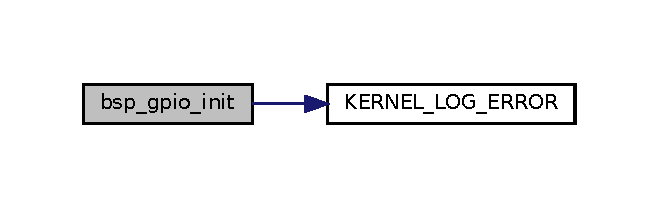
\includegraphics[width=316pt]{bsp__gpio_8h_ac05d93f29cf8cdcd3809298fe5df2f87_cgraph}
\end{center}
\end{figure}
Here is the caller graph for this function\+:\nopagebreak
\begin{figure}[H]
\begin{center}
\leavevmode
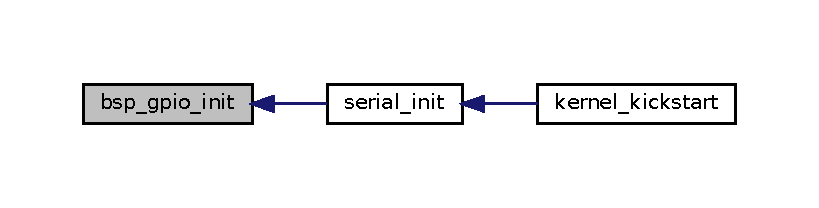
\includegraphics[width=350pt]{bsp__gpio_8h_ac05d93f29cf8cdcd3809298fe5df2f87_icgraph}
\end{center}
\end{figure}

\hypertarget{bsp__power_8h}{}\section{Kernel/\+Sources/arch/board/stm32/f401re/includes/bsp\+\_\+power.h File Reference}
\label{bsp__power_8h}\index{Kernel/\+Sources/arch/board/stm32/f401re/includes/bsp\+\_\+power.\+h@{Kernel/\+Sources/arch/board/stm32/f401re/includes/bsp\+\_\+power.\+h}}
{\ttfamily \#include \char`\"{}error\+\_\+types.\+h\char`\"{}}\newline
{\ttfamily \#include \char`\"{}stdint.\+h\char`\"{}}\newline
Include dependency graph for bsp\+\_\+power.\+h\+:\nopagebreak
\begin{figure}[H]
\begin{center}
\leavevmode
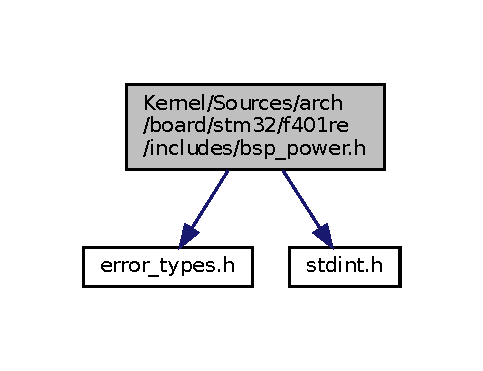
\includegraphics[width=232pt]{bsp__power_8h__incl}
\end{center}
\end{figure}
This graph shows which files directly or indirectly include this file\+:\nopagebreak
\begin{figure}[H]
\begin{center}
\leavevmode
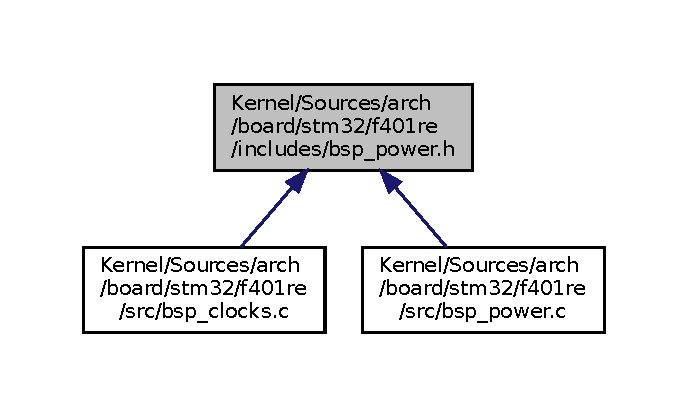
\includegraphics[width=330pt]{bsp__power_8h__dep__incl}
\end{center}
\end{figure}
\subsection*{Macros}
\begin{DoxyCompactItemize}
\item 
\#define \hyperlink{bsp__power_8h_a4b4e210767f8cc202a60b8253350406d}{P\+W\+R\+\_\+\+C\+R\+\_\+\+B\+A\+S\+E\+\_\+\+A\+D\+D\+R\+E\+SS}~0x40007000
\begin{DoxyCompactList}\small\item\em Power Control Register base address. \end{DoxyCompactList}\item 
\#define \hyperlink{bsp__power_8h_a30eb4f51898e3d42222ed18e4f392156}{P\+W\+R\+\_\+\+C\+R\+\_\+\+R\+E\+G\+I\+S\+T\+ER}~((volatile \hyperlink{stdint_8h_a324c5d28c0d82f502a234ab99efac87a}{uint32\+\_\+t}$\ast$)\hyperlink{bsp__power_8h_a4b4e210767f8cc202a60b8253350406d}{P\+W\+R\+\_\+\+C\+R\+\_\+\+B\+A\+S\+E\+\_\+\+A\+D\+D\+R\+E\+SS})
\item 
\#define \hyperlink{bsp__power_8h_a06db718126d979cbf61fc27991514e1a}{P\+W\+R\+\_\+\+C\+R\+\_\+\+V\+O\+S\+\_\+\+M\+A\+SK}~0x0000\+C000
\begin{DoxyCompactList}\small\item\em Power Control Register V\+OS mask. \end{DoxyCompactList}\end{DoxyCompactItemize}
\subsection*{Typedefs}
\begin{DoxyCompactItemize}
\item 
typedef enum \hyperlink{bsp__power_8h_aeab31582495468040935b45b76f06553}{P\+O\+W\+E\+R\+\_\+\+S\+C\+A\+L\+I\+NG} \hyperlink{bsp__power_8h_adbcdf5dee7695e72280aa56c141f5758}{P\+O\+W\+E\+R\+\_\+\+S\+C\+A\+L\+I\+N\+G\+\_\+E}
\begin{DoxyCompactList}\small\item\em Short hand for enum P\+O\+W\+E\+R\+\_\+\+S\+C\+A\+L\+I\+NG. \end{DoxyCompactList}\end{DoxyCompactItemize}
\subsection*{Enumerations}
\begin{DoxyCompactItemize}
\item 
enum \hyperlink{bsp__power_8h_aeab31582495468040935b45b76f06553}{P\+O\+W\+E\+R\+\_\+\+S\+C\+A\+L\+I\+NG} \{ \hyperlink{bsp__power_8h_aeab31582495468040935b45b76f06553a8ddc2bb242e2a77509aad0d808c22339}{P\+O\+W\+E\+R\+\_\+\+S\+C\+A\+L\+I\+N\+G\+\_\+\+M\+O\+D\+E\+\_\+2} = 0x00008000, 
\hyperlink{bsp__power_8h_aeab31582495468040935b45b76f06553ae3d01d01fcb9f3ecf90499f05f5f6652}{P\+O\+W\+E\+R\+\_\+\+S\+C\+A\+L\+I\+N\+G\+\_\+\+M\+O\+D\+E\+\_\+3} = 0x00004000
 \}\begin{DoxyCompactList}\small\item\em Power scaling modes available on the S\+T\+M32\+F401\+RE. \end{DoxyCompactList}
\end{DoxyCompactItemize}
\subsection*{Functions}
\begin{DoxyCompactItemize}
\item 
\hyperlink{error__types_8h_acf146bc98f60f47c79d782f7523e339c}{E\+R\+R\+O\+R\+\_\+\+C\+O\+D\+E\+\_\+E} \hyperlink{bsp__power_8h_abe4bd68d683c1ab3fbc83afb60b36ede}{bsp\+\_\+pwr\+\_\+set\+\_\+scaling} (const \hyperlink{bsp__power_8h_adbcdf5dee7695e72280aa56c141f5758}{P\+O\+W\+E\+R\+\_\+\+S\+C\+A\+L\+I\+N\+G\+\_\+E} pwr\+\_\+scaling)
\begin{DoxyCompactList}\small\item\em Sets the power scaling. \end{DoxyCompactList}\end{DoxyCompactItemize}


\subsection{Macro Definition Documentation}
\mbox{\Hypertarget{bsp__power_8h_a4b4e210767f8cc202a60b8253350406d}\label{bsp__power_8h_a4b4e210767f8cc202a60b8253350406d}} 
\index{bsp\+\_\+power.\+h@{bsp\+\_\+power.\+h}!P\+W\+R\+\_\+\+C\+R\+\_\+\+B\+A\+S\+E\+\_\+\+A\+D\+D\+R\+E\+SS@{P\+W\+R\+\_\+\+C\+R\+\_\+\+B\+A\+S\+E\+\_\+\+A\+D\+D\+R\+E\+SS}}
\index{P\+W\+R\+\_\+\+C\+R\+\_\+\+B\+A\+S\+E\+\_\+\+A\+D\+D\+R\+E\+SS@{P\+W\+R\+\_\+\+C\+R\+\_\+\+B\+A\+S\+E\+\_\+\+A\+D\+D\+R\+E\+SS}!bsp\+\_\+power.\+h@{bsp\+\_\+power.\+h}}
\subsubsection{\texorpdfstring{P\+W\+R\+\_\+\+C\+R\+\_\+\+B\+A\+S\+E\+\_\+\+A\+D\+D\+R\+E\+SS}{PWR\_CR\_BASE\_ADDRESS}}
{\footnotesize\ttfamily \#define P\+W\+R\+\_\+\+C\+R\+\_\+\+B\+A\+S\+E\+\_\+\+A\+D\+D\+R\+E\+SS~0x40007000}



Power Control Register base address. 



Definition at line 27 of file bsp\+\_\+power.\+h.

\mbox{\Hypertarget{bsp__power_8h_a30eb4f51898e3d42222ed18e4f392156}\label{bsp__power_8h_a30eb4f51898e3d42222ed18e4f392156}} 
\index{bsp\+\_\+power.\+h@{bsp\+\_\+power.\+h}!P\+W\+R\+\_\+\+C\+R\+\_\+\+R\+E\+G\+I\+S\+T\+ER@{P\+W\+R\+\_\+\+C\+R\+\_\+\+R\+E\+G\+I\+S\+T\+ER}}
\index{P\+W\+R\+\_\+\+C\+R\+\_\+\+R\+E\+G\+I\+S\+T\+ER@{P\+W\+R\+\_\+\+C\+R\+\_\+\+R\+E\+G\+I\+S\+T\+ER}!bsp\+\_\+power.\+h@{bsp\+\_\+power.\+h}}
\subsubsection{\texorpdfstring{P\+W\+R\+\_\+\+C\+R\+\_\+\+R\+E\+G\+I\+S\+T\+ER}{PWR\_CR\_REGISTER}}
{\footnotesize\ttfamily \#define P\+W\+R\+\_\+\+C\+R\+\_\+\+R\+E\+G\+I\+S\+T\+ER~((volatile \hyperlink{stdint_8h_a324c5d28c0d82f502a234ab99efac87a}{uint32\+\_\+t}$\ast$)\hyperlink{bsp__power_8h_a4b4e210767f8cc202a60b8253350406d}{P\+W\+R\+\_\+\+C\+R\+\_\+\+B\+A\+S\+E\+\_\+\+A\+D\+D\+R\+E\+SS})}



Definition at line 28 of file bsp\+\_\+power.\+h.

\mbox{\Hypertarget{bsp__power_8h_a06db718126d979cbf61fc27991514e1a}\label{bsp__power_8h_a06db718126d979cbf61fc27991514e1a}} 
\index{bsp\+\_\+power.\+h@{bsp\+\_\+power.\+h}!P\+W\+R\+\_\+\+C\+R\+\_\+\+V\+O\+S\+\_\+\+M\+A\+SK@{P\+W\+R\+\_\+\+C\+R\+\_\+\+V\+O\+S\+\_\+\+M\+A\+SK}}
\index{P\+W\+R\+\_\+\+C\+R\+\_\+\+V\+O\+S\+\_\+\+M\+A\+SK@{P\+W\+R\+\_\+\+C\+R\+\_\+\+V\+O\+S\+\_\+\+M\+A\+SK}!bsp\+\_\+power.\+h@{bsp\+\_\+power.\+h}}
\subsubsection{\texorpdfstring{P\+W\+R\+\_\+\+C\+R\+\_\+\+V\+O\+S\+\_\+\+M\+A\+SK}{PWR\_CR\_VOS\_MASK}}
{\footnotesize\ttfamily \#define P\+W\+R\+\_\+\+C\+R\+\_\+\+V\+O\+S\+\_\+\+M\+A\+SK~0x0000\+C000}



Power Control Register V\+OS mask. 



Definition at line 31 of file bsp\+\_\+power.\+h.



\subsection{Typedef Documentation}
\mbox{\Hypertarget{bsp__power_8h_adbcdf5dee7695e72280aa56c141f5758}\label{bsp__power_8h_adbcdf5dee7695e72280aa56c141f5758}} 
\index{bsp\+\_\+power.\+h@{bsp\+\_\+power.\+h}!P\+O\+W\+E\+R\+\_\+\+S\+C\+A\+L\+I\+N\+G\+\_\+E@{P\+O\+W\+E\+R\+\_\+\+S\+C\+A\+L\+I\+N\+G\+\_\+E}}
\index{P\+O\+W\+E\+R\+\_\+\+S\+C\+A\+L\+I\+N\+G\+\_\+E@{P\+O\+W\+E\+R\+\_\+\+S\+C\+A\+L\+I\+N\+G\+\_\+E}!bsp\+\_\+power.\+h@{bsp\+\_\+power.\+h}}
\subsubsection{\texorpdfstring{P\+O\+W\+E\+R\+\_\+\+S\+C\+A\+L\+I\+N\+G\+\_\+E}{POWER\_SCALING\_E}}
{\footnotesize\ttfamily typedef enum \hyperlink{bsp__power_8h_aeab31582495468040935b45b76f06553}{P\+O\+W\+E\+R\+\_\+\+S\+C\+A\+L\+I\+NG} \hyperlink{bsp__power_8h_adbcdf5dee7695e72280aa56c141f5758}{P\+O\+W\+E\+R\+\_\+\+S\+C\+A\+L\+I\+N\+G\+\_\+E}}



Short hand for enum P\+O\+W\+E\+R\+\_\+\+S\+C\+A\+L\+I\+NG. 



Definition at line 47 of file bsp\+\_\+power.\+h.



\subsection{Enumeration Type Documentation}
\mbox{\Hypertarget{bsp__power_8h_aeab31582495468040935b45b76f06553}\label{bsp__power_8h_aeab31582495468040935b45b76f06553}} 
\index{bsp\+\_\+power.\+h@{bsp\+\_\+power.\+h}!P\+O\+W\+E\+R\+\_\+\+S\+C\+A\+L\+I\+NG@{P\+O\+W\+E\+R\+\_\+\+S\+C\+A\+L\+I\+NG}}
\index{P\+O\+W\+E\+R\+\_\+\+S\+C\+A\+L\+I\+NG@{P\+O\+W\+E\+R\+\_\+\+S\+C\+A\+L\+I\+NG}!bsp\+\_\+power.\+h@{bsp\+\_\+power.\+h}}
\subsubsection{\texorpdfstring{P\+O\+W\+E\+R\+\_\+\+S\+C\+A\+L\+I\+NG}{POWER\_SCALING}}
{\footnotesize\ttfamily enum \hyperlink{bsp__power_8h_aeab31582495468040935b45b76f06553}{P\+O\+W\+E\+R\+\_\+\+S\+C\+A\+L\+I\+NG}}



Power scaling modes available on the S\+T\+M32\+F401\+RE. 

\begin{DoxyEnumFields}{Enumerator}
\raisebox{\heightof{T}}[0pt][0pt]{\index{P\+O\+W\+E\+R\+\_\+\+S\+C\+A\+L\+I\+N\+G\+\_\+\+M\+O\+D\+E\+\_\+2@{P\+O\+W\+E\+R\+\_\+\+S\+C\+A\+L\+I\+N\+G\+\_\+\+M\+O\+D\+E\+\_\+2}!bsp\+\_\+power.\+h@{bsp\+\_\+power.\+h}}\index{bsp\+\_\+power.\+h@{bsp\+\_\+power.\+h}!P\+O\+W\+E\+R\+\_\+\+S\+C\+A\+L\+I\+N\+G\+\_\+\+M\+O\+D\+E\+\_\+2@{P\+O\+W\+E\+R\+\_\+\+S\+C\+A\+L\+I\+N\+G\+\_\+\+M\+O\+D\+E\+\_\+2}}}\mbox{\Hypertarget{bsp__power_8h_aeab31582495468040935b45b76f06553a8ddc2bb242e2a77509aad0d808c22339}\label{bsp__power_8h_aeab31582495468040935b45b76f06553a8ddc2bb242e2a77509aad0d808c22339}} 
P\+O\+W\+E\+R\+\_\+\+S\+C\+A\+L\+I\+N\+G\+\_\+\+M\+O\+D\+E\+\_\+2&Power scaling mode 2. \\
\hline

\raisebox{\heightof{T}}[0pt][0pt]{\index{P\+O\+W\+E\+R\+\_\+\+S\+C\+A\+L\+I\+N\+G\+\_\+\+M\+O\+D\+E\+\_\+3@{P\+O\+W\+E\+R\+\_\+\+S\+C\+A\+L\+I\+N\+G\+\_\+\+M\+O\+D\+E\+\_\+3}!bsp\+\_\+power.\+h@{bsp\+\_\+power.\+h}}\index{bsp\+\_\+power.\+h@{bsp\+\_\+power.\+h}!P\+O\+W\+E\+R\+\_\+\+S\+C\+A\+L\+I\+N\+G\+\_\+\+M\+O\+D\+E\+\_\+3@{P\+O\+W\+E\+R\+\_\+\+S\+C\+A\+L\+I\+N\+G\+\_\+\+M\+O\+D\+E\+\_\+3}}}\mbox{\Hypertarget{bsp__power_8h_aeab31582495468040935b45b76f06553ae3d01d01fcb9f3ecf90499f05f5f6652}\label{bsp__power_8h_aeab31582495468040935b45b76f06553ae3d01d01fcb9f3ecf90499f05f5f6652}} 
P\+O\+W\+E\+R\+\_\+\+S\+C\+A\+L\+I\+N\+G\+\_\+\+M\+O\+D\+E\+\_\+3&Power scaling mode 3. \\
\hline

\end{DoxyEnumFields}


Definition at line 38 of file bsp\+\_\+power.\+h.


\begin{DoxyCode}
39 \{
41     \hyperlink{bsp__power_8h_aeab31582495468040935b45b76f06553a8ddc2bb242e2a77509aad0d808c22339}{POWER\_SCALING\_MODE\_2} = 0x00008000,
43     \hyperlink{bsp__power_8h_aeab31582495468040935b45b76f06553ae3d01d01fcb9f3ecf90499f05f5f6652}{POWER\_SCALING\_MODE\_3} = 0x00004000
44 \};
\end{DoxyCode}


\subsection{Function Documentation}
\mbox{\Hypertarget{bsp__power_8h_abe4bd68d683c1ab3fbc83afb60b36ede}\label{bsp__power_8h_abe4bd68d683c1ab3fbc83afb60b36ede}} 
\index{bsp\+\_\+power.\+h@{bsp\+\_\+power.\+h}!bsp\+\_\+pwr\+\_\+set\+\_\+scaling@{bsp\+\_\+pwr\+\_\+set\+\_\+scaling}}
\index{bsp\+\_\+pwr\+\_\+set\+\_\+scaling@{bsp\+\_\+pwr\+\_\+set\+\_\+scaling}!bsp\+\_\+power.\+h@{bsp\+\_\+power.\+h}}
\subsubsection{\texorpdfstring{bsp\+\_\+pwr\+\_\+set\+\_\+scaling()}{bsp\_pwr\_set\_scaling()}}
{\footnotesize\ttfamily \hyperlink{error__types_8h_acf146bc98f60f47c79d782f7523e339c}{E\+R\+R\+O\+R\+\_\+\+C\+O\+D\+E\+\_\+E} bsp\+\_\+pwr\+\_\+set\+\_\+scaling (\begin{DoxyParamCaption}\item[{const \hyperlink{bsp__power_8h_adbcdf5dee7695e72280aa56c141f5758}{P\+O\+W\+E\+R\+\_\+\+S\+C\+A\+L\+I\+N\+G\+\_\+E}}]{pwr\+\_\+scaling }\end{DoxyParamCaption})}



Sets the power scaling. 

Sets the power scaling based on the values passed in paramter. The scaling conforms to the values defined by the reference manual. If the value does not conform, the function has no effect and returns an error code.


\begin{DoxyParams}{Parameters}
{\em pwr\+\_\+scaling} & The scaling factor configuration.\\
\hline
\end{DoxyParams}
\begin{DoxyReturn}{Returns}
N\+O\+\_\+\+E\+R\+R\+OR is returned in case of success. Otherwise an error code is returned. Please refer to the list of the standard error codes. 
\end{DoxyReturn}


Definition at line 33 of file bsp\+\_\+power.\+c.


\begin{DoxyCode}
34 \{
35     \textcolor{comment}{/* Sets the power scaling value, we don't apply mask verification because 
}
36 \textcolor{comment}{     * the POWER\_SCALING\_E enumeration should already contain the right values.
}
37 \textcolor{comment}{     */}
38     *\hyperlink{bsp__power_8h_a30eb4f51898e3d42222ed18e4f392156}{PWR\_CR\_REGISTER} = (*\hyperlink{bsp__power_8h_a30eb4f51898e3d42222ed18e4f392156}{PWR\_CR\_REGISTER} & ~
      \hyperlink{bsp__power_8h_a06db718126d979cbf61fc27991514e1a}{PWR\_CR\_VOS\_MASK}) | pwr\_scaling;
39 
40     \textcolor{comment}{/* Delay to ensure bit update */}
41     \textcolor{keywordflow}{while}((*\hyperlink{bsp__power_8h_a30eb4f51898e3d42222ed18e4f392156}{PWR\_CR\_REGISTER} & \hyperlink{bsp__power_8h_a06db718126d979cbf61fc27991514e1a}{PWR\_CR\_VOS\_MASK}) != pwr\_scaling);
42 
43 \textcolor{preprocessor}{#if KERNEL\_LOG\_LEVEL >= INFO\_LOG\_LEVEL
}
44     KERNEL\_LOG\_INFO(\textcolor{stringliteral}{"Power scaling mode changed"}, 
45                     pwr\_scaling, 
46                     \textcolor{keyword}{sizeof}(pwr\_scaling), 
47                     \hyperlink{error__types_8h_a4db9ee29f2ff83c71567c12f6bfbf28cabf350750d0d4fabd8954c0f1e9bbae94}{NO\_ERROR});
48 \textcolor{preprocessor}{#endif
}
49 
50     \textcolor{keywordflow}{return} \hyperlink{error__types_8h_a4db9ee29f2ff83c71567c12f6bfbf28cabf350750d0d4fabd8954c0f1e9bbae94}{NO\_ERROR};
51 \}
\end{DoxyCode}
Here is the caller graph for this function\+:\nopagebreak
\begin{figure}[H]
\begin{center}
\leavevmode
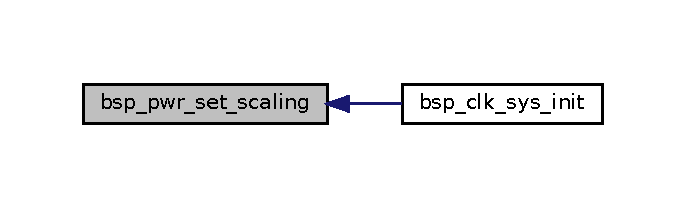
\includegraphics[width=329pt]{bsp__power_8h_abe4bd68d683c1ab3fbc83afb60b36ede_icgraph}
\end{center}
\end{figure}

\hypertarget{bsp__usart_8h}{}\section{Kernel/\+Sources/arch/board/stm32/f401re/includes/bsp\+\_\+usart.h File Reference}
\label{bsp__usart_8h}\index{Kernel/\+Sources/arch/board/stm32/f401re/includes/bsp\+\_\+usart.\+h@{Kernel/\+Sources/arch/board/stm32/f401re/includes/bsp\+\_\+usart.\+h}}
{\ttfamily \#include \char`\"{}error\+\_\+types.\+h\char`\"{}}\newline
Include dependency graph for bsp\+\_\+usart.\+h\+:\nopagebreak
\begin{figure}[H]
\begin{center}
\leavevmode
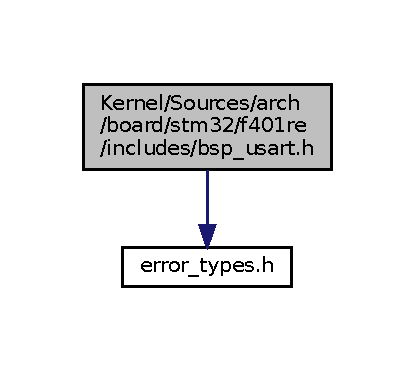
\includegraphics[width=199pt]{bsp__usart_8h__incl}
\end{center}
\end{figure}
This graph shows which files directly or indirectly include this file\+:\nopagebreak
\begin{figure}[H]
\begin{center}
\leavevmode
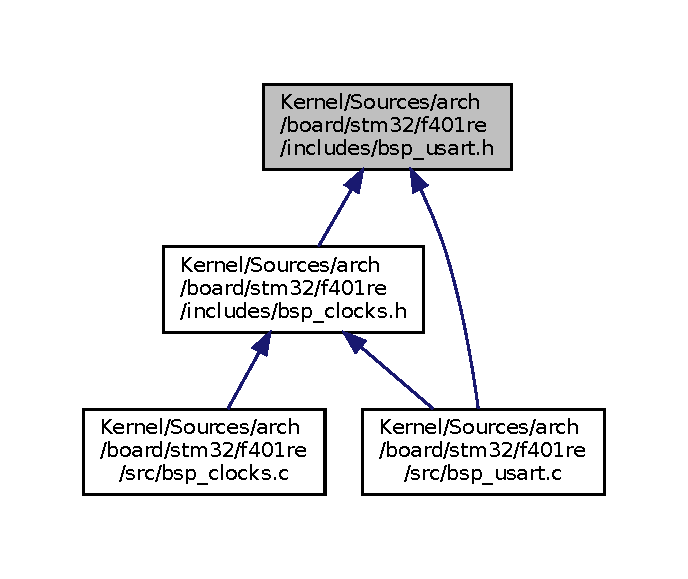
\includegraphics[width=330pt]{bsp__usart_8h__dep__incl}
\end{center}
\end{figure}
\subsection*{Macros}
\begin{DoxyCompactItemize}
\item 
\#define \hyperlink{bsp__usart_8h_ad38e1f3a398c5dca4a14ca3c08b277f1}{U\+S\+A\+R\+T1\+\_\+\+S\+R\+\_\+\+A\+D\+D\+R\+E\+SS}~0x40011000
\begin{DoxyCompactList}\small\item\em U\+S\+A\+R\+T1 Status register address. \end{DoxyCompactList}\item 
\#define \hyperlink{bsp__usart_8h_a4b215072b6db4ffa8a1dcb4d42d9cebd}{U\+S\+A\+R\+T1\+\_\+\+D\+R\+\_\+\+A\+D\+D\+R\+E\+SS}~0x40011004
\begin{DoxyCompactList}\small\item\em U\+S\+A\+R\+T1 Data register address. \end{DoxyCompactList}\item 
\#define \hyperlink{bsp__usart_8h_abcaf3524a9622c5cec6d5d70027c5d15}{U\+S\+A\+R\+T1\+\_\+\+B\+R\+R\+\_\+\+A\+D\+D\+R\+E\+SS}~0x40011008
\begin{DoxyCompactList}\small\item\em U\+S\+A\+R\+T1 Baudrate register address. \end{DoxyCompactList}\item 
\#define \hyperlink{bsp__usart_8h_a7e3cbb9c3b7b3967719512ff9df7d632}{U\+S\+A\+R\+T1\+\_\+\+C\+R1\+\_\+\+A\+D\+D\+R\+E\+SS}~0x4001100C
\begin{DoxyCompactList}\small\item\em U\+S\+A\+R\+T1 Control register 1 address. \end{DoxyCompactList}\item 
\#define \hyperlink{bsp__usart_8h_a88337dffb1ca6564662b6965a5b4c3f6}{U\+S\+A\+R\+T1\+\_\+\+C\+R1\+\_\+\+R\+E\+G\+I\+S\+T\+ER}~((volatile \hyperlink{stdint_8h_a324c5d28c0d82f502a234ab99efac87a}{uint32\+\_\+t}$\ast$)\hyperlink{bsp__usart_8h_a7e3cbb9c3b7b3967719512ff9df7d632}{U\+S\+A\+R\+T1\+\_\+\+C\+R1\+\_\+\+A\+D\+D\+R\+E\+SS})
\item 
\#define \hyperlink{bsp__usart_8h_a5130cce25ab86fc32b7846b2dcbc9abf}{U\+S\+A\+R\+T1\+\_\+\+C\+R2\+\_\+\+A\+D\+D\+R\+E\+SS}~0x40011010
\begin{DoxyCompactList}\small\item\em U\+S\+A\+R\+T1 Control register 2 address. \end{DoxyCompactList}\item 
\#define \hyperlink{bsp__usart_8h_a04b5bd4552470522cddb75322bb9e4a1}{U\+S\+A\+R\+T1\+\_\+\+C\+R3\+\_\+\+A\+D\+D\+R\+E\+SS}~0x40011014
\begin{DoxyCompactList}\small\item\em U\+S\+A\+R\+T1 Control register 3 address. \end{DoxyCompactList}\item 
\#define \hyperlink{bsp__usart_8h_a2117f1f16db6b5616b02589c4b5f7206}{U\+S\+A\+R\+T2\+\_\+\+S\+R\+\_\+\+A\+D\+D\+R\+E\+SS}~0x40004400
\begin{DoxyCompactList}\small\item\em U\+S\+A\+R\+T2 Status register address. \end{DoxyCompactList}\item 
\#define \hyperlink{bsp__usart_8h_aa902cd686824df937532dbdb8a9c9dac}{U\+S\+A\+R\+T2\+\_\+\+S\+R\+\_\+\+R\+E\+G\+I\+S\+T\+ER}~((volatile \hyperlink{stdint_8h_a324c5d28c0d82f502a234ab99efac87a}{uint32\+\_\+t}$\ast$)\hyperlink{bsp__usart_8h_a2117f1f16db6b5616b02589c4b5f7206}{U\+S\+A\+R\+T2\+\_\+\+S\+R\+\_\+\+A\+D\+D\+R\+E\+SS})
\item 
\#define \hyperlink{bsp__usart_8h_a85f05f3739b08e7d34238220b544b081}{U\+S\+A\+R\+T2\+\_\+\+D\+R\+\_\+\+A\+D\+D\+R\+E\+SS}~0x40004404
\begin{DoxyCompactList}\small\item\em U\+S\+A\+R\+T2 Data register address. \end{DoxyCompactList}\item 
\#define \hyperlink{bsp__usart_8h_a8e09469004e7199b63ac9df19afd41a5}{U\+S\+A\+R\+T2\+\_\+\+D\+R\+\_\+\+R\+E\+G\+I\+S\+T\+ER}~((volatile \hyperlink{stdint_8h_a324c5d28c0d82f502a234ab99efac87a}{uint32\+\_\+t}$\ast$)\hyperlink{bsp__usart_8h_a85f05f3739b08e7d34238220b544b081}{U\+S\+A\+R\+T2\+\_\+\+D\+R\+\_\+\+A\+D\+D\+R\+E\+SS})
\item 
\#define \hyperlink{bsp__usart_8h_a02ff054c09f139a38369680f85c1b9e4}{U\+S\+A\+R\+T2\+\_\+\+B\+R\+R\+\_\+\+A\+D\+D\+R\+E\+SS}~0x40004408
\begin{DoxyCompactList}\small\item\em U\+S\+A\+R\+T2 Baudrate register address. \end{DoxyCompactList}\item 
\#define \hyperlink{bsp__usart_8h_a551a35cf294b360d96b14bac0aa81c28}{U\+S\+A\+R\+T2\+\_\+\+C\+R1\+\_\+\+A\+D\+D\+R\+E\+SS}~0x4000440C
\begin{DoxyCompactList}\small\item\em U\+S\+A\+R\+T2 Control register 1 address. \end{DoxyCompactList}\item 
\#define \hyperlink{bsp__usart_8h_aa2ab178d47851e6114531471bc8831bd}{U\+S\+A\+R\+T2\+\_\+\+C\+R1\+\_\+\+R\+E\+G\+I\+S\+T\+ER}~((volatile \hyperlink{stdint_8h_a324c5d28c0d82f502a234ab99efac87a}{uint32\+\_\+t}$\ast$)\hyperlink{bsp__usart_8h_a551a35cf294b360d96b14bac0aa81c28}{U\+S\+A\+R\+T2\+\_\+\+C\+R1\+\_\+\+A\+D\+D\+R\+E\+SS})
\item 
\#define \hyperlink{bsp__usart_8h_aa130d46de6c5714614654179f9b690ca}{U\+S\+A\+R\+T2\+\_\+\+C\+R2\+\_\+\+A\+D\+D\+R\+E\+SS}~0x40004410
\begin{DoxyCompactList}\small\item\em U\+S\+A\+R\+T2 Control register 2 address. \end{DoxyCompactList}\item 
\#define \hyperlink{bsp__usart_8h_a4aceb0927ac1c8ec7adad8e44a0d626a}{U\+S\+A\+R\+T2\+\_\+\+C\+R3\+\_\+\+A\+D\+D\+R\+E\+SS}~0x40004414
\begin{DoxyCompactList}\small\item\em U\+S\+A\+R\+T2 Control register 3 address. \end{DoxyCompactList}\item 
\#define \hyperlink{bsp__usart_8h_af50aeabf02cb4c9e8afe57edb769b1d9}{U\+S\+A\+R\+T6\+\_\+\+S\+R\+\_\+\+A\+D\+D\+R\+E\+SS}~0x40011400
\begin{DoxyCompactList}\small\item\em U\+S\+A\+R\+T6 Status register address. \end{DoxyCompactList}\item 
\#define \hyperlink{bsp__usart_8h_a76ef7c7d267cdeaa05f642e1e7b2f657}{U\+S\+A\+R\+T6\+\_\+\+D\+R\+\_\+\+A\+D\+D\+R\+E\+SS}~0x40011404
\begin{DoxyCompactList}\small\item\em U\+S\+A\+R\+T6 Data register address. \end{DoxyCompactList}\item 
\#define \hyperlink{bsp__usart_8h_a8089788317790f6633511039cb7d50b8}{U\+S\+A\+R\+T6\+\_\+\+B\+R\+R\+\_\+\+A\+D\+D\+R\+E\+SS}~0x40011408
\begin{DoxyCompactList}\small\item\em U\+S\+A\+R\+T6 Baudrate register address. \end{DoxyCompactList}\item 
\#define \hyperlink{bsp__usart_8h_a52e23572285d44dea63aff07039d248e}{U\+S\+A\+R\+T6\+\_\+\+C\+R1\+\_\+\+A\+D\+D\+R\+E\+SS}~0x4001140C
\begin{DoxyCompactList}\small\item\em U\+S\+A\+R\+T6 Control register 1 address. \end{DoxyCompactList}\item 
\#define \hyperlink{bsp__usart_8h_a8ef2bb343a29f32b70ff7cb3a04f4199}{U\+S\+A\+R\+T6\+\_\+\+C\+R1\+\_\+\+R\+E\+G\+I\+S\+T\+ER}~((volatile \hyperlink{stdint_8h_a324c5d28c0d82f502a234ab99efac87a}{uint32\+\_\+t}$\ast$)\hyperlink{bsp__usart_8h_a52e23572285d44dea63aff07039d248e}{U\+S\+A\+R\+T6\+\_\+\+C\+R1\+\_\+\+A\+D\+D\+R\+E\+SS})
\item 
\#define \hyperlink{bsp__usart_8h_a94170d0ce631976cd1daefcb320a1815}{U\+S\+A\+R\+T6\+\_\+\+C\+R2\+\_\+\+A\+D\+D\+R\+E\+SS}~0x40011410
\begin{DoxyCompactList}\small\item\em U\+S\+A\+R\+T6 Control register 2 address. \end{DoxyCompactList}\item 
\#define \hyperlink{bsp__usart_8h_aa5de805e5b75dd00bb77531e7273ad14}{U\+S\+A\+R\+T6\+\_\+\+C\+R3\+\_\+\+A\+D\+D\+R\+E\+SS}~0x40011414
\begin{DoxyCompactList}\small\item\em U\+S\+A\+R\+T6 Control register 3 address. \end{DoxyCompactList}\item 
\#define \hyperlink{bsp__usart_8h_a65e9cddf0890113d405342f1d8b5b980}{U\+S\+A\+R\+T\+\_\+\+S\+R\+\_\+\+T\+XE}~0x00000080
\begin{DoxyCompactList}\small\item\em U\+S\+A\+RT status register transmission ready flag. \end{DoxyCompactList}\item 
\#define \hyperlink{bsp__usart_8h_aed6caeb0cb48f1a7b34090f31a92a8e2}{U\+S\+A\+R\+T\+\_\+\+C\+R1\+\_\+\+O\+V\+E\+R8}~0x00008000
\begin{DoxyCompactList}\small\item\em U\+S\+A\+RT control register 1 oversampling by 8 flag. \end{DoxyCompactList}\item 
\#define \hyperlink{bsp__usart_8h_a2bb650676aaae4a5203f372d497d5947}{U\+S\+A\+R\+T\+\_\+\+C\+R1\+\_\+\+UE}~0x00002000
\begin{DoxyCompactList}\small\item\em U\+S\+A\+RT control register 1 usart enable flag. \end{DoxyCompactList}\item 
\#define \hyperlink{bsp__usart_8h_a95f0288b9c6aaeca7cb6550a2e6833e2}{U\+S\+A\+R\+T\+\_\+\+C\+R1\+\_\+M}~0x00001000
\begin{DoxyCompactList}\small\item\em U\+S\+A\+RT control register 1 word length flag. \end{DoxyCompactList}\item 
\#define \hyperlink{bsp__usart_8h_ad831dfc169fcf14b7284984dbecf322d}{U\+S\+A\+R\+T\+\_\+\+C\+R1\+\_\+\+W\+A\+KE}~0x00000800
\begin{DoxyCompactList}\small\item\em U\+S\+A\+RT control register 1 wakeup flag. \end{DoxyCompactList}\item 
\#define \hyperlink{bsp__usart_8h_a60f8fcf084f9a8514efafb617c70b074}{U\+S\+A\+R\+T\+\_\+\+C\+R1\+\_\+\+P\+CE}~0x00000400
\begin{DoxyCompactList}\small\item\em U\+S\+A\+RT control register 1 parity control flag. \end{DoxyCompactList}\item 
\#define \hyperlink{bsp__usart_8h_a2e159d36ab2c93a2c1942df60e9eebbe}{U\+S\+A\+R\+T\+\_\+\+C\+R1\+\_\+\+PS}~0x00000200
\begin{DoxyCompactList}\small\item\em U\+S\+A\+RT control register 1 parity type flag. \end{DoxyCompactList}\item 
\#define \hyperlink{bsp__usart_8h_a27405d413b6d355ccdb076d52fef6875}{U\+S\+A\+R\+T\+\_\+\+C\+R1\+\_\+\+P\+E\+IE}~0x00000100
\begin{DoxyCompactList}\small\item\em U\+S\+A\+RT control register 1 PE interrupt enable flag. \end{DoxyCompactList}\item 
\#define \hyperlink{bsp__usart_8h_a70422871d15f974b464365e7fe1877e9}{U\+S\+A\+R\+T\+\_\+\+C\+R1\+\_\+\+T\+X\+E\+IE}~0x00000080
\begin{DoxyCompactList}\small\item\em U\+S\+A\+RT control register 1 T\+XE interrupt enable flag. \end{DoxyCompactList}\item 
\#define \hyperlink{bsp__usart_8h_aa17130690a1ca95b972429eb64d4254e}{U\+S\+A\+R\+T\+\_\+\+C\+R1\+\_\+\+T\+C\+IE}~0x00000040
\begin{DoxyCompactList}\small\item\em U\+S\+A\+RT control register 1 TX complete interrupt enable flag. \end{DoxyCompactList}\item 
\#define \hyperlink{bsp__usart_8h_a91118f867adfdb2e805beea86666de04}{U\+S\+A\+R\+T\+\_\+\+C\+R1\+\_\+\+R\+X\+N\+E\+IE}~0x00000020
\begin{DoxyCompactList}\small\item\em U\+S\+A\+RT control register 1 R\+X\+NE interrupt enable flag. \end{DoxyCompactList}\item 
\#define \hyperlink{bsp__usart_8h_a5221d09eebd12445a20f221bf98066f8}{U\+S\+A\+R\+T\+\_\+\+C\+R1\+\_\+\+I\+D\+L\+E\+IE}~0x00000010
\begin{DoxyCompactList}\small\item\em U\+S\+A\+RT control register 1 I\+D\+LE interrupt enable flag. \end{DoxyCompactList}\item 
\#define \hyperlink{bsp__usart_8h_ade7f090b04fd78b755b43357ecaa9622}{U\+S\+A\+R\+T\+\_\+\+C\+R1\+\_\+\+TE}~0x00000008
\begin{DoxyCompactList}\small\item\em U\+S\+A\+RT control register 1 transmiter enable flag. \end{DoxyCompactList}\item 
\#define \hyperlink{bsp__usart_8h_ada0d5d407a22264de847bc1b40a17aeb}{U\+S\+A\+R\+T\+\_\+\+C\+R1\+\_\+\+RE}~0x00000004
\begin{DoxyCompactList}\small\item\em U\+S\+A\+RT control register 1 receiver enable flag. \end{DoxyCompactList}\item 
\#define \hyperlink{bsp__usart_8h_aa7d61ab5a4e2beaa3f591c56bd15a27b}{U\+S\+A\+R\+T\+\_\+\+C\+R1\+\_\+\+R\+WU}~0x00000002
\begin{DoxyCompactList}\small\item\em U\+S\+A\+RT control register 1 receiver wakeup flag. \end{DoxyCompactList}\item 
\#define \hyperlink{bsp__usart_8h_ac457c519baa28359ab7959fbe0c5cda1}{U\+S\+A\+R\+T\+\_\+\+C\+R1\+\_\+\+S\+BK}~0x00000001
\begin{DoxyCompactList}\small\item\em U\+S\+A\+RT control register 1 send break flag. \end{DoxyCompactList}\item 
\#define \hyperlink{bsp__usart_8h_ac8931efa62c29d92f5c0ec5a05f907ef}{U\+S\+A\+R\+T\+\_\+\+C\+R2\+\_\+\+L\+I\+N\+EN}~0x00004000
\begin{DoxyCompactList}\small\item\em U\+S\+A\+RT control register 2 L\+IN mode enable flag. \end{DoxyCompactList}\item 
\#define \hyperlink{bsp__usart_8h_a41e7bdb66e99fb64359cd105d624d41c}{U\+S\+A\+R\+T\+\_\+\+C\+R2\+\_\+\+S\+T\+O\+P\+\_\+05}~0x00001000
\begin{DoxyCompactList}\small\item\em U\+S\+A\+RT control register 2 0.\+5 stop bit field. \end{DoxyCompactList}\item 
\#define \hyperlink{bsp__usart_8h_a2b24d14f0e5d1c76c878b08aad44d02b}{U\+S\+A\+R\+T\+\_\+\+C\+R2\+\_\+\+S\+T\+O\+P\+\_\+1}~0x00000000
\begin{DoxyCompactList}\small\item\em U\+S\+A\+RT control register 2 1 stop bit field. \end{DoxyCompactList}\item 
\#define \hyperlink{bsp__usart_8h_a57f01ae62391c4e1f82e899d8f765858}{U\+S\+A\+R\+T\+\_\+\+C\+R2\+\_\+\+S\+T\+O\+P\+\_\+15}~0x00003000
\begin{DoxyCompactList}\small\item\em U\+S\+A\+RT control register 2 1.\+5 stop bits field. \end{DoxyCompactList}\item 
\#define \hyperlink{bsp__usart_8h_a1792b89d6790744140059546bad805e9}{U\+S\+A\+R\+T\+\_\+\+C\+R2\+\_\+\+S\+T\+O\+P\+\_\+2}~0x00002000
\begin{DoxyCompactList}\small\item\em U\+S\+A\+RT control register 2 2 stop bits field. \end{DoxyCompactList}\item 
\#define \hyperlink{bsp__usart_8h_a42a396cde02ffa0c4d3fd9817b6af853}{U\+S\+A\+R\+T\+\_\+\+C\+R2\+\_\+\+C\+L\+K\+EN}~0x00000800
\begin{DoxyCompactList}\small\item\em U\+S\+A\+RT control register 2 clock enable flag. \end{DoxyCompactList}\item 
\#define \hyperlink{bsp__usart_8h_afbb4336ac93d94d4e78f9fb7b3a0dc68}{U\+S\+A\+R\+T\+\_\+\+C\+R2\+\_\+\+C\+P\+OL}~0x00000400
\begin{DoxyCompactList}\small\item\em U\+S\+A\+RT control register 2 clock polarity flag. \end{DoxyCompactList}\item 
\#define \hyperlink{bsp__usart_8h_a362976ce813e58310399d113d2cf09cb}{U\+S\+A\+R\+T\+\_\+\+C\+R2\+\_\+\+C\+P\+HA}~0x00000200
\begin{DoxyCompactList}\small\item\em U\+S\+A\+RT control register 2 clock phase flag. \end{DoxyCompactList}\item 
\#define \hyperlink{bsp__usart_8h_a4a62e93ae7864e89622bdd92508b615e}{U\+S\+A\+R\+T\+\_\+\+C\+R2\+\_\+\+L\+B\+CL}~0x00000100
\begin{DoxyCompactList}\small\item\em U\+S\+A\+RT control register 2 last bit clock pulse flag. \end{DoxyCompactList}\item 
\#define \hyperlink{bsp__usart_8h_af98769bed28dfd2b222e6884e464f9d2}{U\+S\+A\+R\+T\+\_\+\+C\+R2\+\_\+\+L\+B\+IE}~0x00000040
\begin{DoxyCompactList}\small\item\em U\+S\+A\+RT control register 2 L\+IN break detect interrupt enable flag. \end{DoxyCompactList}\item 
\#define \hyperlink{bsp__usart_8h_a539ea2e20b534b2c742e3194f2ad5a5c}{U\+S\+A\+R\+T\+\_\+\+C\+R2\+\_\+\+L\+BL}~0x00000020
\begin{DoxyCompactList}\small\item\em U\+S\+A\+RT control register 2 L\+IN break detect length flag. \end{DoxyCompactList}\item 
\#define \hyperlink{bsp__usart_8h_ae20ff98868e1e2fec55f2141b5a353bd}{U\+S\+A\+R\+T\+\_\+\+C\+R2\+\_\+\+S\+T\+O\+P\+\_\+\+M\+A\+SK}~0x00003000
\begin{DoxyCompactList}\small\item\em U\+S\+A\+RT control register 2 stop bits field mask. \end{DoxyCompactList}\item 
\#define \hyperlink{bsp__usart_8h_a8abd4cdca00f61296bc3a84a59992dd3}{U\+S\+A\+R\+T\+\_\+\+C\+R2\+\_\+\+A\+D\+D\+R\+\_\+\+M\+A\+SK}~0x0000000F
\begin{DoxyCompactList}\small\item\em U\+S\+A\+RT control register 2 address field mask. \end{DoxyCompactList}\item 
\#define \hyperlink{bsp__usart_8h_a9a96fb1a7beab602cbc8cb0393593826}{U\+S\+A\+R\+T\+\_\+\+C\+R3\+\_\+\+O\+N\+E\+B\+IT}~0x00000800
\begin{DoxyCompactList}\small\item\em U\+S\+A\+RT control register 3 one sample bit method enable flag. \end{DoxyCompactList}\item 
\#define \hyperlink{bsp__usart_8h_a636d5ec2e9556949fc68d13ad45a1e90}{U\+S\+A\+R\+T\+\_\+\+C\+R3\+\_\+\+C\+T\+S\+IE}~0x00000400
\begin{DoxyCompactList}\small\item\em U\+S\+A\+RT control register 3 C\+TS interrupt enable flag. \end{DoxyCompactList}\item 
\#define \hyperlink{bsp__usart_8h_aa125f026b1ca2d76eab48b191baed265}{U\+S\+A\+R\+T\+\_\+\+C\+R3\+\_\+\+C\+T\+SE}~0x00000200
\begin{DoxyCompactList}\small\item\em U\+S\+A\+RT control register 3 C\+TS enable flag. \end{DoxyCompactList}\item 
\#define \hyperlink{bsp__usart_8h_a7c5d6fcd84a4728cda578a0339b4cac2}{U\+S\+A\+R\+T\+\_\+\+C\+R3\+\_\+\+R\+T\+SE}~0x00000100
\begin{DoxyCompactList}\small\item\em U\+S\+A\+RT control register 3 R\+TS enable flag. \end{DoxyCompactList}\item 
\#define \hyperlink{bsp__usart_8h_a5bb515d3814d448f84e2c98bf44f3993}{U\+S\+A\+R\+T\+\_\+\+C\+R3\+\_\+\+D\+M\+AT}~0x00000080
\begin{DoxyCompactList}\small\item\em U\+S\+A\+RT control register 3 D\+MA transmitter enable flag. \end{DoxyCompactList}\item 
\#define \hyperlink{bsp__usart_8h_aff130f15493c765353ec2fd605667c5a}{U\+S\+A\+R\+T\+\_\+\+C\+R3\+\_\+\+D\+M\+AR}~0x00000040
\begin{DoxyCompactList}\small\item\em U\+S\+A\+RT control register 3 D\+MA receiver enable flag. \end{DoxyCompactList}\item 
\#define \hyperlink{bsp__usart_8h_a9180b9249a26988f71d4bb2b0c3eec27}{U\+S\+A\+R\+T\+\_\+\+C\+R3\+\_\+\+S\+C\+EN}~0x00000020
\begin{DoxyCompactList}\small\item\em U\+S\+A\+RT control register 3 smartcard mode enable flag. \end{DoxyCompactList}\item 
\#define \hyperlink{bsp__usart_8h_a3f3b70b2ee9ff0b59e952fd7ab04373c}{U\+S\+A\+R\+T\+\_\+\+C\+R3\+\_\+\+N\+A\+CK}~0x00000010
\begin{DoxyCompactList}\small\item\em U\+S\+A\+RT control register 3 smartcard N\+A\+CK enable flag. \end{DoxyCompactList}\item 
\#define \hyperlink{bsp__usart_8h_ac71129810fab0b46d91161a39e3f8d01}{U\+S\+A\+R\+T\+\_\+\+C\+R3\+\_\+\+H\+D\+S\+EL}~0x00000008
\begin{DoxyCompactList}\small\item\em U\+S\+A\+RT control register 3 half duplex selection flag. \end{DoxyCompactList}\item 
\#define \hyperlink{bsp__usart_8h_a22af8d399f1adda62e31186f0309af80}{U\+S\+A\+R\+T\+\_\+\+C\+R3\+\_\+\+I\+R\+LP}~0x00000004
\begin{DoxyCompactList}\small\item\em U\+S\+A\+RT control register 3 Ir\+DA low power flag. \end{DoxyCompactList}\item 
\#define \hyperlink{bsp__usart_8h_a31c66373bfbae7724c836ac63b8411dd}{U\+S\+A\+R\+T\+\_\+\+C\+R3\+\_\+\+I\+R\+EN}~0x00000002
\begin{DoxyCompactList}\small\item\em U\+S\+A\+RT control register 3 Ir\+DA enable flag. \end{DoxyCompactList}\item 
\#define \hyperlink{bsp__usart_8h_aaed1a39c551b1641128f81893ff558d0}{U\+S\+A\+R\+T\+\_\+\+C\+R3\+\_\+\+E\+IE}~0x00000001
\begin{DoxyCompactList}\small\item\em U\+S\+A\+RT control register 3 error interrupt enable flag. \end{DoxyCompactList}\item 
\#define \hyperlink{bsp__usart_8h_a9c527a46a70f29b45da0d016dd07a3e8}{U\+S\+A\+R\+T\+\_\+\+B\+R\+R\+\_\+\+D\+I\+V\+\_\+\+M\+A\+N\+T\+\_\+\+O\+F\+F\+S\+ET}~4
\begin{DoxyCompactList}\small\item\em B\+RR divider mantissa field offset. \end{DoxyCompactList}\end{DoxyCompactItemize}
\subsection*{Typedefs}
\begin{DoxyCompactItemize}
\item 
typedef enum \hyperlink{bsp__usart_8h_a58f9be3820e29e0fbf00e2466c3ee768}{U\+S\+A\+R\+T\+\_\+\+I\+D\+E\+N\+T\+I\+F\+I\+ER} \hyperlink{bsp__usart_8h_a594f9d90a9a3875660da4512fb208cf9}{U\+S\+A\+R\+T\+\_\+\+I\+D\+E\+N\+T\+I\+F\+I\+E\+R\+\_\+E}
\begin{DoxyCompactList}\small\item\em Short hand for enum U\+S\+A\+R\+T\+\_\+\+I\+D\+E\+N\+T\+I\+F\+I\+ER. \end{DoxyCompactList}\end{DoxyCompactItemize}
\subsection*{Enumerations}
\begin{DoxyCompactItemize}
\item 
enum \hyperlink{bsp__usart_8h_a58f9be3820e29e0fbf00e2466c3ee768}{U\+S\+A\+R\+T\+\_\+\+I\+D\+E\+N\+T\+I\+F\+I\+ER} \{ \hyperlink{bsp__usart_8h_a58f9be3820e29e0fbf00e2466c3ee768a512d550c862eac9ad45d923508bb0f7d}{U\+S\+A\+R\+T\+\_\+\+I\+D\+\_\+1} = 0, 
\hyperlink{bsp__usart_8h_a58f9be3820e29e0fbf00e2466c3ee768abb138542d801249fd01ec62c34f52cff}{U\+S\+A\+R\+T\+\_\+\+I\+D\+\_\+2} = 1, 
\hyperlink{bsp__usart_8h_a58f9be3820e29e0fbf00e2466c3ee768afd45e5de3678cbcada70f46bde327479}{U\+S\+A\+R\+T\+\_\+\+I\+D\+\_\+6} = 3
 \}\begin{DoxyCompactList}\small\item\em U\+S\+A\+RT identifier used to differenciated the U\+S\+A\+R\+Ts present on the S\+T\+M32\+F401\+RE board. \end{DoxyCompactList}
\end{DoxyCompactItemize}


\subsection{Macro Definition Documentation}
\mbox{\Hypertarget{bsp__usart_8h_abcaf3524a9622c5cec6d5d70027c5d15}\label{bsp__usart_8h_abcaf3524a9622c5cec6d5d70027c5d15}} 
\index{bsp\+\_\+usart.\+h@{bsp\+\_\+usart.\+h}!U\+S\+A\+R\+T1\+\_\+\+B\+R\+R\+\_\+\+A\+D\+D\+R\+E\+SS@{U\+S\+A\+R\+T1\+\_\+\+B\+R\+R\+\_\+\+A\+D\+D\+R\+E\+SS}}
\index{U\+S\+A\+R\+T1\+\_\+\+B\+R\+R\+\_\+\+A\+D\+D\+R\+E\+SS@{U\+S\+A\+R\+T1\+\_\+\+B\+R\+R\+\_\+\+A\+D\+D\+R\+E\+SS}!bsp\+\_\+usart.\+h@{bsp\+\_\+usart.\+h}}
\subsubsection{\texorpdfstring{U\+S\+A\+R\+T1\+\_\+\+B\+R\+R\+\_\+\+A\+D\+D\+R\+E\+SS}{USART1\_BRR\_ADDRESS}}
{\footnotesize\ttfamily \#define U\+S\+A\+R\+T1\+\_\+\+B\+R\+R\+\_\+\+A\+D\+D\+R\+E\+SS~0x40011008}



U\+S\+A\+R\+T1 Baudrate register address. 



Definition at line 32 of file bsp\+\_\+usart.\+h.

\mbox{\Hypertarget{bsp__usart_8h_a7e3cbb9c3b7b3967719512ff9df7d632}\label{bsp__usart_8h_a7e3cbb9c3b7b3967719512ff9df7d632}} 
\index{bsp\+\_\+usart.\+h@{bsp\+\_\+usart.\+h}!U\+S\+A\+R\+T1\+\_\+\+C\+R1\+\_\+\+A\+D\+D\+R\+E\+SS@{U\+S\+A\+R\+T1\+\_\+\+C\+R1\+\_\+\+A\+D\+D\+R\+E\+SS}}
\index{U\+S\+A\+R\+T1\+\_\+\+C\+R1\+\_\+\+A\+D\+D\+R\+E\+SS@{U\+S\+A\+R\+T1\+\_\+\+C\+R1\+\_\+\+A\+D\+D\+R\+E\+SS}!bsp\+\_\+usart.\+h@{bsp\+\_\+usart.\+h}}
\subsubsection{\texorpdfstring{U\+S\+A\+R\+T1\+\_\+\+C\+R1\+\_\+\+A\+D\+D\+R\+E\+SS}{USART1\_CR1\_ADDRESS}}
{\footnotesize\ttfamily \#define U\+S\+A\+R\+T1\+\_\+\+C\+R1\+\_\+\+A\+D\+D\+R\+E\+SS~0x4001100C}



U\+S\+A\+R\+T1 Control register 1 address. 



Definition at line 34 of file bsp\+\_\+usart.\+h.

\mbox{\Hypertarget{bsp__usart_8h_a88337dffb1ca6564662b6965a5b4c3f6}\label{bsp__usart_8h_a88337dffb1ca6564662b6965a5b4c3f6}} 
\index{bsp\+\_\+usart.\+h@{bsp\+\_\+usart.\+h}!U\+S\+A\+R\+T1\+\_\+\+C\+R1\+\_\+\+R\+E\+G\+I\+S\+T\+ER@{U\+S\+A\+R\+T1\+\_\+\+C\+R1\+\_\+\+R\+E\+G\+I\+S\+T\+ER}}
\index{U\+S\+A\+R\+T1\+\_\+\+C\+R1\+\_\+\+R\+E\+G\+I\+S\+T\+ER@{U\+S\+A\+R\+T1\+\_\+\+C\+R1\+\_\+\+R\+E\+G\+I\+S\+T\+ER}!bsp\+\_\+usart.\+h@{bsp\+\_\+usart.\+h}}
\subsubsection{\texorpdfstring{U\+S\+A\+R\+T1\+\_\+\+C\+R1\+\_\+\+R\+E\+G\+I\+S\+T\+ER}{USART1\_CR1\_REGISTER}}
{\footnotesize\ttfamily \#define U\+S\+A\+R\+T1\+\_\+\+C\+R1\+\_\+\+R\+E\+G\+I\+S\+T\+ER~((volatile \hyperlink{stdint_8h_a324c5d28c0d82f502a234ab99efac87a}{uint32\+\_\+t}$\ast$)\hyperlink{bsp__usart_8h_a7e3cbb9c3b7b3967719512ff9df7d632}{U\+S\+A\+R\+T1\+\_\+\+C\+R1\+\_\+\+A\+D\+D\+R\+E\+SS})}



Definition at line 35 of file bsp\+\_\+usart.\+h.

\mbox{\Hypertarget{bsp__usart_8h_a5130cce25ab86fc32b7846b2dcbc9abf}\label{bsp__usart_8h_a5130cce25ab86fc32b7846b2dcbc9abf}} 
\index{bsp\+\_\+usart.\+h@{bsp\+\_\+usart.\+h}!U\+S\+A\+R\+T1\+\_\+\+C\+R2\+\_\+\+A\+D\+D\+R\+E\+SS@{U\+S\+A\+R\+T1\+\_\+\+C\+R2\+\_\+\+A\+D\+D\+R\+E\+SS}}
\index{U\+S\+A\+R\+T1\+\_\+\+C\+R2\+\_\+\+A\+D\+D\+R\+E\+SS@{U\+S\+A\+R\+T1\+\_\+\+C\+R2\+\_\+\+A\+D\+D\+R\+E\+SS}!bsp\+\_\+usart.\+h@{bsp\+\_\+usart.\+h}}
\subsubsection{\texorpdfstring{U\+S\+A\+R\+T1\+\_\+\+C\+R2\+\_\+\+A\+D\+D\+R\+E\+SS}{USART1\_CR2\_ADDRESS}}
{\footnotesize\ttfamily \#define U\+S\+A\+R\+T1\+\_\+\+C\+R2\+\_\+\+A\+D\+D\+R\+E\+SS~0x40011010}



U\+S\+A\+R\+T1 Control register 2 address. 



Definition at line 37 of file bsp\+\_\+usart.\+h.

\mbox{\Hypertarget{bsp__usart_8h_a04b5bd4552470522cddb75322bb9e4a1}\label{bsp__usart_8h_a04b5bd4552470522cddb75322bb9e4a1}} 
\index{bsp\+\_\+usart.\+h@{bsp\+\_\+usart.\+h}!U\+S\+A\+R\+T1\+\_\+\+C\+R3\+\_\+\+A\+D\+D\+R\+E\+SS@{U\+S\+A\+R\+T1\+\_\+\+C\+R3\+\_\+\+A\+D\+D\+R\+E\+SS}}
\index{U\+S\+A\+R\+T1\+\_\+\+C\+R3\+\_\+\+A\+D\+D\+R\+E\+SS@{U\+S\+A\+R\+T1\+\_\+\+C\+R3\+\_\+\+A\+D\+D\+R\+E\+SS}!bsp\+\_\+usart.\+h@{bsp\+\_\+usart.\+h}}
\subsubsection{\texorpdfstring{U\+S\+A\+R\+T1\+\_\+\+C\+R3\+\_\+\+A\+D\+D\+R\+E\+SS}{USART1\_CR3\_ADDRESS}}
{\footnotesize\ttfamily \#define U\+S\+A\+R\+T1\+\_\+\+C\+R3\+\_\+\+A\+D\+D\+R\+E\+SS~0x40011014}



U\+S\+A\+R\+T1 Control register 3 address. 



Definition at line 39 of file bsp\+\_\+usart.\+h.

\mbox{\Hypertarget{bsp__usart_8h_a4b215072b6db4ffa8a1dcb4d42d9cebd}\label{bsp__usart_8h_a4b215072b6db4ffa8a1dcb4d42d9cebd}} 
\index{bsp\+\_\+usart.\+h@{bsp\+\_\+usart.\+h}!U\+S\+A\+R\+T1\+\_\+\+D\+R\+\_\+\+A\+D\+D\+R\+E\+SS@{U\+S\+A\+R\+T1\+\_\+\+D\+R\+\_\+\+A\+D\+D\+R\+E\+SS}}
\index{U\+S\+A\+R\+T1\+\_\+\+D\+R\+\_\+\+A\+D\+D\+R\+E\+SS@{U\+S\+A\+R\+T1\+\_\+\+D\+R\+\_\+\+A\+D\+D\+R\+E\+SS}!bsp\+\_\+usart.\+h@{bsp\+\_\+usart.\+h}}
\subsubsection{\texorpdfstring{U\+S\+A\+R\+T1\+\_\+\+D\+R\+\_\+\+A\+D\+D\+R\+E\+SS}{USART1\_DR\_ADDRESS}}
{\footnotesize\ttfamily \#define U\+S\+A\+R\+T1\+\_\+\+D\+R\+\_\+\+A\+D\+D\+R\+E\+SS~0x40011004}



U\+S\+A\+R\+T1 Data register address. 



Definition at line 30 of file bsp\+\_\+usart.\+h.

\mbox{\Hypertarget{bsp__usart_8h_ad38e1f3a398c5dca4a14ca3c08b277f1}\label{bsp__usart_8h_ad38e1f3a398c5dca4a14ca3c08b277f1}} 
\index{bsp\+\_\+usart.\+h@{bsp\+\_\+usart.\+h}!U\+S\+A\+R\+T1\+\_\+\+S\+R\+\_\+\+A\+D\+D\+R\+E\+SS@{U\+S\+A\+R\+T1\+\_\+\+S\+R\+\_\+\+A\+D\+D\+R\+E\+SS}}
\index{U\+S\+A\+R\+T1\+\_\+\+S\+R\+\_\+\+A\+D\+D\+R\+E\+SS@{U\+S\+A\+R\+T1\+\_\+\+S\+R\+\_\+\+A\+D\+D\+R\+E\+SS}!bsp\+\_\+usart.\+h@{bsp\+\_\+usart.\+h}}
\subsubsection{\texorpdfstring{U\+S\+A\+R\+T1\+\_\+\+S\+R\+\_\+\+A\+D\+D\+R\+E\+SS}{USART1\_SR\_ADDRESS}}
{\footnotesize\ttfamily \#define U\+S\+A\+R\+T1\+\_\+\+S\+R\+\_\+\+A\+D\+D\+R\+E\+SS~0x40011000}



U\+S\+A\+R\+T1 Status register address. 



Definition at line 28 of file bsp\+\_\+usart.\+h.

\mbox{\Hypertarget{bsp__usart_8h_a02ff054c09f139a38369680f85c1b9e4}\label{bsp__usart_8h_a02ff054c09f139a38369680f85c1b9e4}} 
\index{bsp\+\_\+usart.\+h@{bsp\+\_\+usart.\+h}!U\+S\+A\+R\+T2\+\_\+\+B\+R\+R\+\_\+\+A\+D\+D\+R\+E\+SS@{U\+S\+A\+R\+T2\+\_\+\+B\+R\+R\+\_\+\+A\+D\+D\+R\+E\+SS}}
\index{U\+S\+A\+R\+T2\+\_\+\+B\+R\+R\+\_\+\+A\+D\+D\+R\+E\+SS@{U\+S\+A\+R\+T2\+\_\+\+B\+R\+R\+\_\+\+A\+D\+D\+R\+E\+SS}!bsp\+\_\+usart.\+h@{bsp\+\_\+usart.\+h}}
\subsubsection{\texorpdfstring{U\+S\+A\+R\+T2\+\_\+\+B\+R\+R\+\_\+\+A\+D\+D\+R\+E\+SS}{USART2\_BRR\_ADDRESS}}
{\footnotesize\ttfamily \#define U\+S\+A\+R\+T2\+\_\+\+B\+R\+R\+\_\+\+A\+D\+D\+R\+E\+SS~0x40004408}



U\+S\+A\+R\+T2 Baudrate register address. 



Definition at line 48 of file bsp\+\_\+usart.\+h.

\mbox{\Hypertarget{bsp__usart_8h_a551a35cf294b360d96b14bac0aa81c28}\label{bsp__usart_8h_a551a35cf294b360d96b14bac0aa81c28}} 
\index{bsp\+\_\+usart.\+h@{bsp\+\_\+usart.\+h}!U\+S\+A\+R\+T2\+\_\+\+C\+R1\+\_\+\+A\+D\+D\+R\+E\+SS@{U\+S\+A\+R\+T2\+\_\+\+C\+R1\+\_\+\+A\+D\+D\+R\+E\+SS}}
\index{U\+S\+A\+R\+T2\+\_\+\+C\+R1\+\_\+\+A\+D\+D\+R\+E\+SS@{U\+S\+A\+R\+T2\+\_\+\+C\+R1\+\_\+\+A\+D\+D\+R\+E\+SS}!bsp\+\_\+usart.\+h@{bsp\+\_\+usart.\+h}}
\subsubsection{\texorpdfstring{U\+S\+A\+R\+T2\+\_\+\+C\+R1\+\_\+\+A\+D\+D\+R\+E\+SS}{USART2\_CR1\_ADDRESS}}
{\footnotesize\ttfamily \#define U\+S\+A\+R\+T2\+\_\+\+C\+R1\+\_\+\+A\+D\+D\+R\+E\+SS~0x4000440C}



U\+S\+A\+R\+T2 Control register 1 address. 



Definition at line 50 of file bsp\+\_\+usart.\+h.

\mbox{\Hypertarget{bsp__usart_8h_aa2ab178d47851e6114531471bc8831bd}\label{bsp__usart_8h_aa2ab178d47851e6114531471bc8831bd}} 
\index{bsp\+\_\+usart.\+h@{bsp\+\_\+usart.\+h}!U\+S\+A\+R\+T2\+\_\+\+C\+R1\+\_\+\+R\+E\+G\+I\+S\+T\+ER@{U\+S\+A\+R\+T2\+\_\+\+C\+R1\+\_\+\+R\+E\+G\+I\+S\+T\+ER}}
\index{U\+S\+A\+R\+T2\+\_\+\+C\+R1\+\_\+\+R\+E\+G\+I\+S\+T\+ER@{U\+S\+A\+R\+T2\+\_\+\+C\+R1\+\_\+\+R\+E\+G\+I\+S\+T\+ER}!bsp\+\_\+usart.\+h@{bsp\+\_\+usart.\+h}}
\subsubsection{\texorpdfstring{U\+S\+A\+R\+T2\+\_\+\+C\+R1\+\_\+\+R\+E\+G\+I\+S\+T\+ER}{USART2\_CR1\_REGISTER}}
{\footnotesize\ttfamily \#define U\+S\+A\+R\+T2\+\_\+\+C\+R1\+\_\+\+R\+E\+G\+I\+S\+T\+ER~((volatile \hyperlink{stdint_8h_a324c5d28c0d82f502a234ab99efac87a}{uint32\+\_\+t}$\ast$)\hyperlink{bsp__usart_8h_a551a35cf294b360d96b14bac0aa81c28}{U\+S\+A\+R\+T2\+\_\+\+C\+R1\+\_\+\+A\+D\+D\+R\+E\+SS})}



Definition at line 51 of file bsp\+\_\+usart.\+h.

\mbox{\Hypertarget{bsp__usart_8h_aa130d46de6c5714614654179f9b690ca}\label{bsp__usart_8h_aa130d46de6c5714614654179f9b690ca}} 
\index{bsp\+\_\+usart.\+h@{bsp\+\_\+usart.\+h}!U\+S\+A\+R\+T2\+\_\+\+C\+R2\+\_\+\+A\+D\+D\+R\+E\+SS@{U\+S\+A\+R\+T2\+\_\+\+C\+R2\+\_\+\+A\+D\+D\+R\+E\+SS}}
\index{U\+S\+A\+R\+T2\+\_\+\+C\+R2\+\_\+\+A\+D\+D\+R\+E\+SS@{U\+S\+A\+R\+T2\+\_\+\+C\+R2\+\_\+\+A\+D\+D\+R\+E\+SS}!bsp\+\_\+usart.\+h@{bsp\+\_\+usart.\+h}}
\subsubsection{\texorpdfstring{U\+S\+A\+R\+T2\+\_\+\+C\+R2\+\_\+\+A\+D\+D\+R\+E\+SS}{USART2\_CR2\_ADDRESS}}
{\footnotesize\ttfamily \#define U\+S\+A\+R\+T2\+\_\+\+C\+R2\+\_\+\+A\+D\+D\+R\+E\+SS~0x40004410}



U\+S\+A\+R\+T2 Control register 2 address. 



Definition at line 53 of file bsp\+\_\+usart.\+h.

\mbox{\Hypertarget{bsp__usart_8h_a4aceb0927ac1c8ec7adad8e44a0d626a}\label{bsp__usart_8h_a4aceb0927ac1c8ec7adad8e44a0d626a}} 
\index{bsp\+\_\+usart.\+h@{bsp\+\_\+usart.\+h}!U\+S\+A\+R\+T2\+\_\+\+C\+R3\+\_\+\+A\+D\+D\+R\+E\+SS@{U\+S\+A\+R\+T2\+\_\+\+C\+R3\+\_\+\+A\+D\+D\+R\+E\+SS}}
\index{U\+S\+A\+R\+T2\+\_\+\+C\+R3\+\_\+\+A\+D\+D\+R\+E\+SS@{U\+S\+A\+R\+T2\+\_\+\+C\+R3\+\_\+\+A\+D\+D\+R\+E\+SS}!bsp\+\_\+usart.\+h@{bsp\+\_\+usart.\+h}}
\subsubsection{\texorpdfstring{U\+S\+A\+R\+T2\+\_\+\+C\+R3\+\_\+\+A\+D\+D\+R\+E\+SS}{USART2\_CR3\_ADDRESS}}
{\footnotesize\ttfamily \#define U\+S\+A\+R\+T2\+\_\+\+C\+R3\+\_\+\+A\+D\+D\+R\+E\+SS~0x40004414}



U\+S\+A\+R\+T2 Control register 3 address. 



Definition at line 55 of file bsp\+\_\+usart.\+h.

\mbox{\Hypertarget{bsp__usart_8h_a85f05f3739b08e7d34238220b544b081}\label{bsp__usart_8h_a85f05f3739b08e7d34238220b544b081}} 
\index{bsp\+\_\+usart.\+h@{bsp\+\_\+usart.\+h}!U\+S\+A\+R\+T2\+\_\+\+D\+R\+\_\+\+A\+D\+D\+R\+E\+SS@{U\+S\+A\+R\+T2\+\_\+\+D\+R\+\_\+\+A\+D\+D\+R\+E\+SS}}
\index{U\+S\+A\+R\+T2\+\_\+\+D\+R\+\_\+\+A\+D\+D\+R\+E\+SS@{U\+S\+A\+R\+T2\+\_\+\+D\+R\+\_\+\+A\+D\+D\+R\+E\+SS}!bsp\+\_\+usart.\+h@{bsp\+\_\+usart.\+h}}
\subsubsection{\texorpdfstring{U\+S\+A\+R\+T2\+\_\+\+D\+R\+\_\+\+A\+D\+D\+R\+E\+SS}{USART2\_DR\_ADDRESS}}
{\footnotesize\ttfamily \#define U\+S\+A\+R\+T2\+\_\+\+D\+R\+\_\+\+A\+D\+D\+R\+E\+SS~0x40004404}



U\+S\+A\+R\+T2 Data register address. 



Definition at line 45 of file bsp\+\_\+usart.\+h.

\mbox{\Hypertarget{bsp__usart_8h_a8e09469004e7199b63ac9df19afd41a5}\label{bsp__usart_8h_a8e09469004e7199b63ac9df19afd41a5}} 
\index{bsp\+\_\+usart.\+h@{bsp\+\_\+usart.\+h}!U\+S\+A\+R\+T2\+\_\+\+D\+R\+\_\+\+R\+E\+G\+I\+S\+T\+ER@{U\+S\+A\+R\+T2\+\_\+\+D\+R\+\_\+\+R\+E\+G\+I\+S\+T\+ER}}
\index{U\+S\+A\+R\+T2\+\_\+\+D\+R\+\_\+\+R\+E\+G\+I\+S\+T\+ER@{U\+S\+A\+R\+T2\+\_\+\+D\+R\+\_\+\+R\+E\+G\+I\+S\+T\+ER}!bsp\+\_\+usart.\+h@{bsp\+\_\+usart.\+h}}
\subsubsection{\texorpdfstring{U\+S\+A\+R\+T2\+\_\+\+D\+R\+\_\+\+R\+E\+G\+I\+S\+T\+ER}{USART2\_DR\_REGISTER}}
{\footnotesize\ttfamily \#define U\+S\+A\+R\+T2\+\_\+\+D\+R\+\_\+\+R\+E\+G\+I\+S\+T\+ER~((volatile \hyperlink{stdint_8h_a324c5d28c0d82f502a234ab99efac87a}{uint32\+\_\+t}$\ast$)\hyperlink{bsp__usart_8h_a85f05f3739b08e7d34238220b544b081}{U\+S\+A\+R\+T2\+\_\+\+D\+R\+\_\+\+A\+D\+D\+R\+E\+SS})}



Definition at line 46 of file bsp\+\_\+usart.\+h.

\mbox{\Hypertarget{bsp__usart_8h_a2117f1f16db6b5616b02589c4b5f7206}\label{bsp__usart_8h_a2117f1f16db6b5616b02589c4b5f7206}} 
\index{bsp\+\_\+usart.\+h@{bsp\+\_\+usart.\+h}!U\+S\+A\+R\+T2\+\_\+\+S\+R\+\_\+\+A\+D\+D\+R\+E\+SS@{U\+S\+A\+R\+T2\+\_\+\+S\+R\+\_\+\+A\+D\+D\+R\+E\+SS}}
\index{U\+S\+A\+R\+T2\+\_\+\+S\+R\+\_\+\+A\+D\+D\+R\+E\+SS@{U\+S\+A\+R\+T2\+\_\+\+S\+R\+\_\+\+A\+D\+D\+R\+E\+SS}!bsp\+\_\+usart.\+h@{bsp\+\_\+usart.\+h}}
\subsubsection{\texorpdfstring{U\+S\+A\+R\+T2\+\_\+\+S\+R\+\_\+\+A\+D\+D\+R\+E\+SS}{USART2\_SR\_ADDRESS}}
{\footnotesize\ttfamily \#define U\+S\+A\+R\+T2\+\_\+\+S\+R\+\_\+\+A\+D\+D\+R\+E\+SS~0x40004400}



U\+S\+A\+R\+T2 Status register address. 



Definition at line 42 of file bsp\+\_\+usart.\+h.

\mbox{\Hypertarget{bsp__usart_8h_aa902cd686824df937532dbdb8a9c9dac}\label{bsp__usart_8h_aa902cd686824df937532dbdb8a9c9dac}} 
\index{bsp\+\_\+usart.\+h@{bsp\+\_\+usart.\+h}!U\+S\+A\+R\+T2\+\_\+\+S\+R\+\_\+\+R\+E\+G\+I\+S\+T\+ER@{U\+S\+A\+R\+T2\+\_\+\+S\+R\+\_\+\+R\+E\+G\+I\+S\+T\+ER}}
\index{U\+S\+A\+R\+T2\+\_\+\+S\+R\+\_\+\+R\+E\+G\+I\+S\+T\+ER@{U\+S\+A\+R\+T2\+\_\+\+S\+R\+\_\+\+R\+E\+G\+I\+S\+T\+ER}!bsp\+\_\+usart.\+h@{bsp\+\_\+usart.\+h}}
\subsubsection{\texorpdfstring{U\+S\+A\+R\+T2\+\_\+\+S\+R\+\_\+\+R\+E\+G\+I\+S\+T\+ER}{USART2\_SR\_REGISTER}}
{\footnotesize\ttfamily \#define U\+S\+A\+R\+T2\+\_\+\+S\+R\+\_\+\+R\+E\+G\+I\+S\+T\+ER~((volatile \hyperlink{stdint_8h_a324c5d28c0d82f502a234ab99efac87a}{uint32\+\_\+t}$\ast$)\hyperlink{bsp__usart_8h_a2117f1f16db6b5616b02589c4b5f7206}{U\+S\+A\+R\+T2\+\_\+\+S\+R\+\_\+\+A\+D\+D\+R\+E\+SS})}



Definition at line 43 of file bsp\+\_\+usart.\+h.

\mbox{\Hypertarget{bsp__usart_8h_a8089788317790f6633511039cb7d50b8}\label{bsp__usart_8h_a8089788317790f6633511039cb7d50b8}} 
\index{bsp\+\_\+usart.\+h@{bsp\+\_\+usart.\+h}!U\+S\+A\+R\+T6\+\_\+\+B\+R\+R\+\_\+\+A\+D\+D\+R\+E\+SS@{U\+S\+A\+R\+T6\+\_\+\+B\+R\+R\+\_\+\+A\+D\+D\+R\+E\+SS}}
\index{U\+S\+A\+R\+T6\+\_\+\+B\+R\+R\+\_\+\+A\+D\+D\+R\+E\+SS@{U\+S\+A\+R\+T6\+\_\+\+B\+R\+R\+\_\+\+A\+D\+D\+R\+E\+SS}!bsp\+\_\+usart.\+h@{bsp\+\_\+usart.\+h}}
\subsubsection{\texorpdfstring{U\+S\+A\+R\+T6\+\_\+\+B\+R\+R\+\_\+\+A\+D\+D\+R\+E\+SS}{USART6\_BRR\_ADDRESS}}
{\footnotesize\ttfamily \#define U\+S\+A\+R\+T6\+\_\+\+B\+R\+R\+\_\+\+A\+D\+D\+R\+E\+SS~0x40011408}



U\+S\+A\+R\+T6 Baudrate register address. 



Definition at line 62 of file bsp\+\_\+usart.\+h.

\mbox{\Hypertarget{bsp__usart_8h_a52e23572285d44dea63aff07039d248e}\label{bsp__usart_8h_a52e23572285d44dea63aff07039d248e}} 
\index{bsp\+\_\+usart.\+h@{bsp\+\_\+usart.\+h}!U\+S\+A\+R\+T6\+\_\+\+C\+R1\+\_\+\+A\+D\+D\+R\+E\+SS@{U\+S\+A\+R\+T6\+\_\+\+C\+R1\+\_\+\+A\+D\+D\+R\+E\+SS}}
\index{U\+S\+A\+R\+T6\+\_\+\+C\+R1\+\_\+\+A\+D\+D\+R\+E\+SS@{U\+S\+A\+R\+T6\+\_\+\+C\+R1\+\_\+\+A\+D\+D\+R\+E\+SS}!bsp\+\_\+usart.\+h@{bsp\+\_\+usart.\+h}}
\subsubsection{\texorpdfstring{U\+S\+A\+R\+T6\+\_\+\+C\+R1\+\_\+\+A\+D\+D\+R\+E\+SS}{USART6\_CR1\_ADDRESS}}
{\footnotesize\ttfamily \#define U\+S\+A\+R\+T6\+\_\+\+C\+R1\+\_\+\+A\+D\+D\+R\+E\+SS~0x4001140C}



U\+S\+A\+R\+T6 Control register 1 address. 



Definition at line 64 of file bsp\+\_\+usart.\+h.

\mbox{\Hypertarget{bsp__usart_8h_a8ef2bb343a29f32b70ff7cb3a04f4199}\label{bsp__usart_8h_a8ef2bb343a29f32b70ff7cb3a04f4199}} 
\index{bsp\+\_\+usart.\+h@{bsp\+\_\+usart.\+h}!U\+S\+A\+R\+T6\+\_\+\+C\+R1\+\_\+\+R\+E\+G\+I\+S\+T\+ER@{U\+S\+A\+R\+T6\+\_\+\+C\+R1\+\_\+\+R\+E\+G\+I\+S\+T\+ER}}
\index{U\+S\+A\+R\+T6\+\_\+\+C\+R1\+\_\+\+R\+E\+G\+I\+S\+T\+ER@{U\+S\+A\+R\+T6\+\_\+\+C\+R1\+\_\+\+R\+E\+G\+I\+S\+T\+ER}!bsp\+\_\+usart.\+h@{bsp\+\_\+usart.\+h}}
\subsubsection{\texorpdfstring{U\+S\+A\+R\+T6\+\_\+\+C\+R1\+\_\+\+R\+E\+G\+I\+S\+T\+ER}{USART6\_CR1\_REGISTER}}
{\footnotesize\ttfamily \#define U\+S\+A\+R\+T6\+\_\+\+C\+R1\+\_\+\+R\+E\+G\+I\+S\+T\+ER~((volatile \hyperlink{stdint_8h_a324c5d28c0d82f502a234ab99efac87a}{uint32\+\_\+t}$\ast$)\hyperlink{bsp__usart_8h_a52e23572285d44dea63aff07039d248e}{U\+S\+A\+R\+T6\+\_\+\+C\+R1\+\_\+\+A\+D\+D\+R\+E\+SS})}



Definition at line 65 of file bsp\+\_\+usart.\+h.

\mbox{\Hypertarget{bsp__usart_8h_a94170d0ce631976cd1daefcb320a1815}\label{bsp__usart_8h_a94170d0ce631976cd1daefcb320a1815}} 
\index{bsp\+\_\+usart.\+h@{bsp\+\_\+usart.\+h}!U\+S\+A\+R\+T6\+\_\+\+C\+R2\+\_\+\+A\+D\+D\+R\+E\+SS@{U\+S\+A\+R\+T6\+\_\+\+C\+R2\+\_\+\+A\+D\+D\+R\+E\+SS}}
\index{U\+S\+A\+R\+T6\+\_\+\+C\+R2\+\_\+\+A\+D\+D\+R\+E\+SS@{U\+S\+A\+R\+T6\+\_\+\+C\+R2\+\_\+\+A\+D\+D\+R\+E\+SS}!bsp\+\_\+usart.\+h@{bsp\+\_\+usart.\+h}}
\subsubsection{\texorpdfstring{U\+S\+A\+R\+T6\+\_\+\+C\+R2\+\_\+\+A\+D\+D\+R\+E\+SS}{USART6\_CR2\_ADDRESS}}
{\footnotesize\ttfamily \#define U\+S\+A\+R\+T6\+\_\+\+C\+R2\+\_\+\+A\+D\+D\+R\+E\+SS~0x40011410}



U\+S\+A\+R\+T6 Control register 2 address. 



Definition at line 67 of file bsp\+\_\+usart.\+h.

\mbox{\Hypertarget{bsp__usart_8h_aa5de805e5b75dd00bb77531e7273ad14}\label{bsp__usart_8h_aa5de805e5b75dd00bb77531e7273ad14}} 
\index{bsp\+\_\+usart.\+h@{bsp\+\_\+usart.\+h}!U\+S\+A\+R\+T6\+\_\+\+C\+R3\+\_\+\+A\+D\+D\+R\+E\+SS@{U\+S\+A\+R\+T6\+\_\+\+C\+R3\+\_\+\+A\+D\+D\+R\+E\+SS}}
\index{U\+S\+A\+R\+T6\+\_\+\+C\+R3\+\_\+\+A\+D\+D\+R\+E\+SS@{U\+S\+A\+R\+T6\+\_\+\+C\+R3\+\_\+\+A\+D\+D\+R\+E\+SS}!bsp\+\_\+usart.\+h@{bsp\+\_\+usart.\+h}}
\subsubsection{\texorpdfstring{U\+S\+A\+R\+T6\+\_\+\+C\+R3\+\_\+\+A\+D\+D\+R\+E\+SS}{USART6\_CR3\_ADDRESS}}
{\footnotesize\ttfamily \#define U\+S\+A\+R\+T6\+\_\+\+C\+R3\+\_\+\+A\+D\+D\+R\+E\+SS~0x40011414}



U\+S\+A\+R\+T6 Control register 3 address. 



Definition at line 69 of file bsp\+\_\+usart.\+h.

\mbox{\Hypertarget{bsp__usart_8h_a76ef7c7d267cdeaa05f642e1e7b2f657}\label{bsp__usart_8h_a76ef7c7d267cdeaa05f642e1e7b2f657}} 
\index{bsp\+\_\+usart.\+h@{bsp\+\_\+usart.\+h}!U\+S\+A\+R\+T6\+\_\+\+D\+R\+\_\+\+A\+D\+D\+R\+E\+SS@{U\+S\+A\+R\+T6\+\_\+\+D\+R\+\_\+\+A\+D\+D\+R\+E\+SS}}
\index{U\+S\+A\+R\+T6\+\_\+\+D\+R\+\_\+\+A\+D\+D\+R\+E\+SS@{U\+S\+A\+R\+T6\+\_\+\+D\+R\+\_\+\+A\+D\+D\+R\+E\+SS}!bsp\+\_\+usart.\+h@{bsp\+\_\+usart.\+h}}
\subsubsection{\texorpdfstring{U\+S\+A\+R\+T6\+\_\+\+D\+R\+\_\+\+A\+D\+D\+R\+E\+SS}{USART6\_DR\_ADDRESS}}
{\footnotesize\ttfamily \#define U\+S\+A\+R\+T6\+\_\+\+D\+R\+\_\+\+A\+D\+D\+R\+E\+SS~0x40011404}



U\+S\+A\+R\+T6 Data register address. 



Definition at line 60 of file bsp\+\_\+usart.\+h.

\mbox{\Hypertarget{bsp__usart_8h_af50aeabf02cb4c9e8afe57edb769b1d9}\label{bsp__usart_8h_af50aeabf02cb4c9e8afe57edb769b1d9}} 
\index{bsp\+\_\+usart.\+h@{bsp\+\_\+usart.\+h}!U\+S\+A\+R\+T6\+\_\+\+S\+R\+\_\+\+A\+D\+D\+R\+E\+SS@{U\+S\+A\+R\+T6\+\_\+\+S\+R\+\_\+\+A\+D\+D\+R\+E\+SS}}
\index{U\+S\+A\+R\+T6\+\_\+\+S\+R\+\_\+\+A\+D\+D\+R\+E\+SS@{U\+S\+A\+R\+T6\+\_\+\+S\+R\+\_\+\+A\+D\+D\+R\+E\+SS}!bsp\+\_\+usart.\+h@{bsp\+\_\+usart.\+h}}
\subsubsection{\texorpdfstring{U\+S\+A\+R\+T6\+\_\+\+S\+R\+\_\+\+A\+D\+D\+R\+E\+SS}{USART6\_SR\_ADDRESS}}
{\footnotesize\ttfamily \#define U\+S\+A\+R\+T6\+\_\+\+S\+R\+\_\+\+A\+D\+D\+R\+E\+SS~0x40011400}



U\+S\+A\+R\+T6 Status register address. 



Definition at line 58 of file bsp\+\_\+usart.\+h.

\mbox{\Hypertarget{bsp__usart_8h_a9c527a46a70f29b45da0d016dd07a3e8}\label{bsp__usart_8h_a9c527a46a70f29b45da0d016dd07a3e8}} 
\index{bsp\+\_\+usart.\+h@{bsp\+\_\+usart.\+h}!U\+S\+A\+R\+T\+\_\+\+B\+R\+R\+\_\+\+D\+I\+V\+\_\+\+M\+A\+N\+T\+\_\+\+O\+F\+F\+S\+ET@{U\+S\+A\+R\+T\+\_\+\+B\+R\+R\+\_\+\+D\+I\+V\+\_\+\+M\+A\+N\+T\+\_\+\+O\+F\+F\+S\+ET}}
\index{U\+S\+A\+R\+T\+\_\+\+B\+R\+R\+\_\+\+D\+I\+V\+\_\+\+M\+A\+N\+T\+\_\+\+O\+F\+F\+S\+ET@{U\+S\+A\+R\+T\+\_\+\+B\+R\+R\+\_\+\+D\+I\+V\+\_\+\+M\+A\+N\+T\+\_\+\+O\+F\+F\+S\+ET}!bsp\+\_\+usart.\+h@{bsp\+\_\+usart.\+h}}
\subsubsection{\texorpdfstring{U\+S\+A\+R\+T\+\_\+\+B\+R\+R\+\_\+\+D\+I\+V\+\_\+\+M\+A\+N\+T\+\_\+\+O\+F\+F\+S\+ET}{USART\_BRR\_DIV\_MANT\_OFFSET}}
{\footnotesize\ttfamily \#define U\+S\+A\+R\+T\+\_\+\+B\+R\+R\+\_\+\+D\+I\+V\+\_\+\+M\+A\+N\+T\+\_\+\+O\+F\+F\+S\+ET~4}



B\+RR divider mantissa field offset. 



Definition at line 159 of file bsp\+\_\+usart.\+h.

\mbox{\Hypertarget{bsp__usart_8h_a5221d09eebd12445a20f221bf98066f8}\label{bsp__usart_8h_a5221d09eebd12445a20f221bf98066f8}} 
\index{bsp\+\_\+usart.\+h@{bsp\+\_\+usart.\+h}!U\+S\+A\+R\+T\+\_\+\+C\+R1\+\_\+\+I\+D\+L\+E\+IE@{U\+S\+A\+R\+T\+\_\+\+C\+R1\+\_\+\+I\+D\+L\+E\+IE}}
\index{U\+S\+A\+R\+T\+\_\+\+C\+R1\+\_\+\+I\+D\+L\+E\+IE@{U\+S\+A\+R\+T\+\_\+\+C\+R1\+\_\+\+I\+D\+L\+E\+IE}!bsp\+\_\+usart.\+h@{bsp\+\_\+usart.\+h}}
\subsubsection{\texorpdfstring{U\+S\+A\+R\+T\+\_\+\+C\+R1\+\_\+\+I\+D\+L\+E\+IE}{USART\_CR1\_IDLEIE}}
{\footnotesize\ttfamily \#define U\+S\+A\+R\+T\+\_\+\+C\+R1\+\_\+\+I\+D\+L\+E\+IE~0x00000010}



U\+S\+A\+RT control register 1 I\+D\+LE interrupt enable flag. 



Definition at line 95 of file bsp\+\_\+usart.\+h.

\mbox{\Hypertarget{bsp__usart_8h_a95f0288b9c6aaeca7cb6550a2e6833e2}\label{bsp__usart_8h_a95f0288b9c6aaeca7cb6550a2e6833e2}} 
\index{bsp\+\_\+usart.\+h@{bsp\+\_\+usart.\+h}!U\+S\+A\+R\+T\+\_\+\+C\+R1\+\_\+M@{U\+S\+A\+R\+T\+\_\+\+C\+R1\+\_\+M}}
\index{U\+S\+A\+R\+T\+\_\+\+C\+R1\+\_\+M@{U\+S\+A\+R\+T\+\_\+\+C\+R1\+\_\+M}!bsp\+\_\+usart.\+h@{bsp\+\_\+usart.\+h}}
\subsubsection{\texorpdfstring{U\+S\+A\+R\+T\+\_\+\+C\+R1\+\_\+M}{USART\_CR1\_M}}
{\footnotesize\ttfamily \#define U\+S\+A\+R\+T\+\_\+\+C\+R1\+\_\+M~0x00001000}



U\+S\+A\+RT control register 1 word length flag. 



Definition at line 79 of file bsp\+\_\+usart.\+h.

\mbox{\Hypertarget{bsp__usart_8h_aed6caeb0cb48f1a7b34090f31a92a8e2}\label{bsp__usart_8h_aed6caeb0cb48f1a7b34090f31a92a8e2}} 
\index{bsp\+\_\+usart.\+h@{bsp\+\_\+usart.\+h}!U\+S\+A\+R\+T\+\_\+\+C\+R1\+\_\+\+O\+V\+E\+R8@{U\+S\+A\+R\+T\+\_\+\+C\+R1\+\_\+\+O\+V\+E\+R8}}
\index{U\+S\+A\+R\+T\+\_\+\+C\+R1\+\_\+\+O\+V\+E\+R8@{U\+S\+A\+R\+T\+\_\+\+C\+R1\+\_\+\+O\+V\+E\+R8}!bsp\+\_\+usart.\+h@{bsp\+\_\+usart.\+h}}
\subsubsection{\texorpdfstring{U\+S\+A\+R\+T\+\_\+\+C\+R1\+\_\+\+O\+V\+E\+R8}{USART\_CR1\_OVER8}}
{\footnotesize\ttfamily \#define U\+S\+A\+R\+T\+\_\+\+C\+R1\+\_\+\+O\+V\+E\+R8~0x00008000}



U\+S\+A\+RT control register 1 oversampling by 8 flag. 



Definition at line 75 of file bsp\+\_\+usart.\+h.

\mbox{\Hypertarget{bsp__usart_8h_a60f8fcf084f9a8514efafb617c70b074}\label{bsp__usart_8h_a60f8fcf084f9a8514efafb617c70b074}} 
\index{bsp\+\_\+usart.\+h@{bsp\+\_\+usart.\+h}!U\+S\+A\+R\+T\+\_\+\+C\+R1\+\_\+\+P\+CE@{U\+S\+A\+R\+T\+\_\+\+C\+R1\+\_\+\+P\+CE}}
\index{U\+S\+A\+R\+T\+\_\+\+C\+R1\+\_\+\+P\+CE@{U\+S\+A\+R\+T\+\_\+\+C\+R1\+\_\+\+P\+CE}!bsp\+\_\+usart.\+h@{bsp\+\_\+usart.\+h}}
\subsubsection{\texorpdfstring{U\+S\+A\+R\+T\+\_\+\+C\+R1\+\_\+\+P\+CE}{USART\_CR1\_PCE}}
{\footnotesize\ttfamily \#define U\+S\+A\+R\+T\+\_\+\+C\+R1\+\_\+\+P\+CE~0x00000400}



U\+S\+A\+RT control register 1 parity control flag. 



Definition at line 83 of file bsp\+\_\+usart.\+h.

\mbox{\Hypertarget{bsp__usart_8h_a27405d413b6d355ccdb076d52fef6875}\label{bsp__usart_8h_a27405d413b6d355ccdb076d52fef6875}} 
\index{bsp\+\_\+usart.\+h@{bsp\+\_\+usart.\+h}!U\+S\+A\+R\+T\+\_\+\+C\+R1\+\_\+\+P\+E\+IE@{U\+S\+A\+R\+T\+\_\+\+C\+R1\+\_\+\+P\+E\+IE}}
\index{U\+S\+A\+R\+T\+\_\+\+C\+R1\+\_\+\+P\+E\+IE@{U\+S\+A\+R\+T\+\_\+\+C\+R1\+\_\+\+P\+E\+IE}!bsp\+\_\+usart.\+h@{bsp\+\_\+usart.\+h}}
\subsubsection{\texorpdfstring{U\+S\+A\+R\+T\+\_\+\+C\+R1\+\_\+\+P\+E\+IE}{USART\_CR1\_PEIE}}
{\footnotesize\ttfamily \#define U\+S\+A\+R\+T\+\_\+\+C\+R1\+\_\+\+P\+E\+IE~0x00000100}



U\+S\+A\+RT control register 1 PE interrupt enable flag. 



Definition at line 87 of file bsp\+\_\+usart.\+h.

\mbox{\Hypertarget{bsp__usart_8h_a2e159d36ab2c93a2c1942df60e9eebbe}\label{bsp__usart_8h_a2e159d36ab2c93a2c1942df60e9eebbe}} 
\index{bsp\+\_\+usart.\+h@{bsp\+\_\+usart.\+h}!U\+S\+A\+R\+T\+\_\+\+C\+R1\+\_\+\+PS@{U\+S\+A\+R\+T\+\_\+\+C\+R1\+\_\+\+PS}}
\index{U\+S\+A\+R\+T\+\_\+\+C\+R1\+\_\+\+PS@{U\+S\+A\+R\+T\+\_\+\+C\+R1\+\_\+\+PS}!bsp\+\_\+usart.\+h@{bsp\+\_\+usart.\+h}}
\subsubsection{\texorpdfstring{U\+S\+A\+R\+T\+\_\+\+C\+R1\+\_\+\+PS}{USART\_CR1\_PS}}
{\footnotesize\ttfamily \#define U\+S\+A\+R\+T\+\_\+\+C\+R1\+\_\+\+PS~0x00000200}



U\+S\+A\+RT control register 1 parity type flag. 



Definition at line 85 of file bsp\+\_\+usart.\+h.

\mbox{\Hypertarget{bsp__usart_8h_ada0d5d407a22264de847bc1b40a17aeb}\label{bsp__usart_8h_ada0d5d407a22264de847bc1b40a17aeb}} 
\index{bsp\+\_\+usart.\+h@{bsp\+\_\+usart.\+h}!U\+S\+A\+R\+T\+\_\+\+C\+R1\+\_\+\+RE@{U\+S\+A\+R\+T\+\_\+\+C\+R1\+\_\+\+RE}}
\index{U\+S\+A\+R\+T\+\_\+\+C\+R1\+\_\+\+RE@{U\+S\+A\+R\+T\+\_\+\+C\+R1\+\_\+\+RE}!bsp\+\_\+usart.\+h@{bsp\+\_\+usart.\+h}}
\subsubsection{\texorpdfstring{U\+S\+A\+R\+T\+\_\+\+C\+R1\+\_\+\+RE}{USART\_CR1\_RE}}
{\footnotesize\ttfamily \#define U\+S\+A\+R\+T\+\_\+\+C\+R1\+\_\+\+RE~0x00000004}



U\+S\+A\+RT control register 1 receiver enable flag. 



Definition at line 99 of file bsp\+\_\+usart.\+h.

\mbox{\Hypertarget{bsp__usart_8h_aa7d61ab5a4e2beaa3f591c56bd15a27b}\label{bsp__usart_8h_aa7d61ab5a4e2beaa3f591c56bd15a27b}} 
\index{bsp\+\_\+usart.\+h@{bsp\+\_\+usart.\+h}!U\+S\+A\+R\+T\+\_\+\+C\+R1\+\_\+\+R\+WU@{U\+S\+A\+R\+T\+\_\+\+C\+R1\+\_\+\+R\+WU}}
\index{U\+S\+A\+R\+T\+\_\+\+C\+R1\+\_\+\+R\+WU@{U\+S\+A\+R\+T\+\_\+\+C\+R1\+\_\+\+R\+WU}!bsp\+\_\+usart.\+h@{bsp\+\_\+usart.\+h}}
\subsubsection{\texorpdfstring{U\+S\+A\+R\+T\+\_\+\+C\+R1\+\_\+\+R\+WU}{USART\_CR1\_RWU}}
{\footnotesize\ttfamily \#define U\+S\+A\+R\+T\+\_\+\+C\+R1\+\_\+\+R\+WU~0x00000002}



U\+S\+A\+RT control register 1 receiver wakeup flag. 



Definition at line 101 of file bsp\+\_\+usart.\+h.

\mbox{\Hypertarget{bsp__usart_8h_a91118f867adfdb2e805beea86666de04}\label{bsp__usart_8h_a91118f867adfdb2e805beea86666de04}} 
\index{bsp\+\_\+usart.\+h@{bsp\+\_\+usart.\+h}!U\+S\+A\+R\+T\+\_\+\+C\+R1\+\_\+\+R\+X\+N\+E\+IE@{U\+S\+A\+R\+T\+\_\+\+C\+R1\+\_\+\+R\+X\+N\+E\+IE}}
\index{U\+S\+A\+R\+T\+\_\+\+C\+R1\+\_\+\+R\+X\+N\+E\+IE@{U\+S\+A\+R\+T\+\_\+\+C\+R1\+\_\+\+R\+X\+N\+E\+IE}!bsp\+\_\+usart.\+h@{bsp\+\_\+usart.\+h}}
\subsubsection{\texorpdfstring{U\+S\+A\+R\+T\+\_\+\+C\+R1\+\_\+\+R\+X\+N\+E\+IE}{USART\_CR1\_RXNEIE}}
{\footnotesize\ttfamily \#define U\+S\+A\+R\+T\+\_\+\+C\+R1\+\_\+\+R\+X\+N\+E\+IE~0x00000020}



U\+S\+A\+RT control register 1 R\+X\+NE interrupt enable flag. 



Definition at line 93 of file bsp\+\_\+usart.\+h.

\mbox{\Hypertarget{bsp__usart_8h_ac457c519baa28359ab7959fbe0c5cda1}\label{bsp__usart_8h_ac457c519baa28359ab7959fbe0c5cda1}} 
\index{bsp\+\_\+usart.\+h@{bsp\+\_\+usart.\+h}!U\+S\+A\+R\+T\+\_\+\+C\+R1\+\_\+\+S\+BK@{U\+S\+A\+R\+T\+\_\+\+C\+R1\+\_\+\+S\+BK}}
\index{U\+S\+A\+R\+T\+\_\+\+C\+R1\+\_\+\+S\+BK@{U\+S\+A\+R\+T\+\_\+\+C\+R1\+\_\+\+S\+BK}!bsp\+\_\+usart.\+h@{bsp\+\_\+usart.\+h}}
\subsubsection{\texorpdfstring{U\+S\+A\+R\+T\+\_\+\+C\+R1\+\_\+\+S\+BK}{USART\_CR1\_SBK}}
{\footnotesize\ttfamily \#define U\+S\+A\+R\+T\+\_\+\+C\+R1\+\_\+\+S\+BK~0x00000001}



U\+S\+A\+RT control register 1 send break flag. 



Definition at line 103 of file bsp\+\_\+usart.\+h.

\mbox{\Hypertarget{bsp__usart_8h_aa17130690a1ca95b972429eb64d4254e}\label{bsp__usart_8h_aa17130690a1ca95b972429eb64d4254e}} 
\index{bsp\+\_\+usart.\+h@{bsp\+\_\+usart.\+h}!U\+S\+A\+R\+T\+\_\+\+C\+R1\+\_\+\+T\+C\+IE@{U\+S\+A\+R\+T\+\_\+\+C\+R1\+\_\+\+T\+C\+IE}}
\index{U\+S\+A\+R\+T\+\_\+\+C\+R1\+\_\+\+T\+C\+IE@{U\+S\+A\+R\+T\+\_\+\+C\+R1\+\_\+\+T\+C\+IE}!bsp\+\_\+usart.\+h@{bsp\+\_\+usart.\+h}}
\subsubsection{\texorpdfstring{U\+S\+A\+R\+T\+\_\+\+C\+R1\+\_\+\+T\+C\+IE}{USART\_CR1\_TCIE}}
{\footnotesize\ttfamily \#define U\+S\+A\+R\+T\+\_\+\+C\+R1\+\_\+\+T\+C\+IE~0x00000040}



U\+S\+A\+RT control register 1 TX complete interrupt enable flag. 



Definition at line 91 of file bsp\+\_\+usart.\+h.

\mbox{\Hypertarget{bsp__usart_8h_ade7f090b04fd78b755b43357ecaa9622}\label{bsp__usart_8h_ade7f090b04fd78b755b43357ecaa9622}} 
\index{bsp\+\_\+usart.\+h@{bsp\+\_\+usart.\+h}!U\+S\+A\+R\+T\+\_\+\+C\+R1\+\_\+\+TE@{U\+S\+A\+R\+T\+\_\+\+C\+R1\+\_\+\+TE}}
\index{U\+S\+A\+R\+T\+\_\+\+C\+R1\+\_\+\+TE@{U\+S\+A\+R\+T\+\_\+\+C\+R1\+\_\+\+TE}!bsp\+\_\+usart.\+h@{bsp\+\_\+usart.\+h}}
\subsubsection{\texorpdfstring{U\+S\+A\+R\+T\+\_\+\+C\+R1\+\_\+\+TE}{USART\_CR1\_TE}}
{\footnotesize\ttfamily \#define U\+S\+A\+R\+T\+\_\+\+C\+R1\+\_\+\+TE~0x00000008}



U\+S\+A\+RT control register 1 transmiter enable flag. 



Definition at line 97 of file bsp\+\_\+usart.\+h.

\mbox{\Hypertarget{bsp__usart_8h_a70422871d15f974b464365e7fe1877e9}\label{bsp__usart_8h_a70422871d15f974b464365e7fe1877e9}} 
\index{bsp\+\_\+usart.\+h@{bsp\+\_\+usart.\+h}!U\+S\+A\+R\+T\+\_\+\+C\+R1\+\_\+\+T\+X\+E\+IE@{U\+S\+A\+R\+T\+\_\+\+C\+R1\+\_\+\+T\+X\+E\+IE}}
\index{U\+S\+A\+R\+T\+\_\+\+C\+R1\+\_\+\+T\+X\+E\+IE@{U\+S\+A\+R\+T\+\_\+\+C\+R1\+\_\+\+T\+X\+E\+IE}!bsp\+\_\+usart.\+h@{bsp\+\_\+usart.\+h}}
\subsubsection{\texorpdfstring{U\+S\+A\+R\+T\+\_\+\+C\+R1\+\_\+\+T\+X\+E\+IE}{USART\_CR1\_TXEIE}}
{\footnotesize\ttfamily \#define U\+S\+A\+R\+T\+\_\+\+C\+R1\+\_\+\+T\+X\+E\+IE~0x00000080}



U\+S\+A\+RT control register 1 T\+XE interrupt enable flag. 



Definition at line 89 of file bsp\+\_\+usart.\+h.

\mbox{\Hypertarget{bsp__usart_8h_a2bb650676aaae4a5203f372d497d5947}\label{bsp__usart_8h_a2bb650676aaae4a5203f372d497d5947}} 
\index{bsp\+\_\+usart.\+h@{bsp\+\_\+usart.\+h}!U\+S\+A\+R\+T\+\_\+\+C\+R1\+\_\+\+UE@{U\+S\+A\+R\+T\+\_\+\+C\+R1\+\_\+\+UE}}
\index{U\+S\+A\+R\+T\+\_\+\+C\+R1\+\_\+\+UE@{U\+S\+A\+R\+T\+\_\+\+C\+R1\+\_\+\+UE}!bsp\+\_\+usart.\+h@{bsp\+\_\+usart.\+h}}
\subsubsection{\texorpdfstring{U\+S\+A\+R\+T\+\_\+\+C\+R1\+\_\+\+UE}{USART\_CR1\_UE}}
{\footnotesize\ttfamily \#define U\+S\+A\+R\+T\+\_\+\+C\+R1\+\_\+\+UE~0x00002000}



U\+S\+A\+RT control register 1 usart enable flag. 



Definition at line 77 of file bsp\+\_\+usart.\+h.

\mbox{\Hypertarget{bsp__usart_8h_ad831dfc169fcf14b7284984dbecf322d}\label{bsp__usart_8h_ad831dfc169fcf14b7284984dbecf322d}} 
\index{bsp\+\_\+usart.\+h@{bsp\+\_\+usart.\+h}!U\+S\+A\+R\+T\+\_\+\+C\+R1\+\_\+\+W\+A\+KE@{U\+S\+A\+R\+T\+\_\+\+C\+R1\+\_\+\+W\+A\+KE}}
\index{U\+S\+A\+R\+T\+\_\+\+C\+R1\+\_\+\+W\+A\+KE@{U\+S\+A\+R\+T\+\_\+\+C\+R1\+\_\+\+W\+A\+KE}!bsp\+\_\+usart.\+h@{bsp\+\_\+usart.\+h}}
\subsubsection{\texorpdfstring{U\+S\+A\+R\+T\+\_\+\+C\+R1\+\_\+\+W\+A\+KE}{USART\_CR1\_WAKE}}
{\footnotesize\ttfamily \#define U\+S\+A\+R\+T\+\_\+\+C\+R1\+\_\+\+W\+A\+KE~0x00000800}



U\+S\+A\+RT control register 1 wakeup flag. 



Definition at line 81 of file bsp\+\_\+usart.\+h.

\mbox{\Hypertarget{bsp__usart_8h_a8abd4cdca00f61296bc3a84a59992dd3}\label{bsp__usart_8h_a8abd4cdca00f61296bc3a84a59992dd3}} 
\index{bsp\+\_\+usart.\+h@{bsp\+\_\+usart.\+h}!U\+S\+A\+R\+T\+\_\+\+C\+R2\+\_\+\+A\+D\+D\+R\+\_\+\+M\+A\+SK@{U\+S\+A\+R\+T\+\_\+\+C\+R2\+\_\+\+A\+D\+D\+R\+\_\+\+M\+A\+SK}}
\index{U\+S\+A\+R\+T\+\_\+\+C\+R2\+\_\+\+A\+D\+D\+R\+\_\+\+M\+A\+SK@{U\+S\+A\+R\+T\+\_\+\+C\+R2\+\_\+\+A\+D\+D\+R\+\_\+\+M\+A\+SK}!bsp\+\_\+usart.\+h@{bsp\+\_\+usart.\+h}}
\subsubsection{\texorpdfstring{U\+S\+A\+R\+T\+\_\+\+C\+R2\+\_\+\+A\+D\+D\+R\+\_\+\+M\+A\+SK}{USART\_CR2\_ADDR\_MASK}}
{\footnotesize\ttfamily \#define U\+S\+A\+R\+T\+\_\+\+C\+R2\+\_\+\+A\+D\+D\+R\+\_\+\+M\+A\+SK~0x0000000F}



U\+S\+A\+RT control register 2 address field mask. 



Definition at line 131 of file bsp\+\_\+usart.\+h.

\mbox{\Hypertarget{bsp__usart_8h_a42a396cde02ffa0c4d3fd9817b6af853}\label{bsp__usart_8h_a42a396cde02ffa0c4d3fd9817b6af853}} 
\index{bsp\+\_\+usart.\+h@{bsp\+\_\+usart.\+h}!U\+S\+A\+R\+T\+\_\+\+C\+R2\+\_\+\+C\+L\+K\+EN@{U\+S\+A\+R\+T\+\_\+\+C\+R2\+\_\+\+C\+L\+K\+EN}}
\index{U\+S\+A\+R\+T\+\_\+\+C\+R2\+\_\+\+C\+L\+K\+EN@{U\+S\+A\+R\+T\+\_\+\+C\+R2\+\_\+\+C\+L\+K\+EN}!bsp\+\_\+usart.\+h@{bsp\+\_\+usart.\+h}}
\subsubsection{\texorpdfstring{U\+S\+A\+R\+T\+\_\+\+C\+R2\+\_\+\+C\+L\+K\+EN}{USART\_CR2\_CLKEN}}
{\footnotesize\ttfamily \#define U\+S\+A\+R\+T\+\_\+\+C\+R2\+\_\+\+C\+L\+K\+EN~0x00000800}



U\+S\+A\+RT control register 2 clock enable flag. 



Definition at line 116 of file bsp\+\_\+usart.\+h.

\mbox{\Hypertarget{bsp__usart_8h_a362976ce813e58310399d113d2cf09cb}\label{bsp__usart_8h_a362976ce813e58310399d113d2cf09cb}} 
\index{bsp\+\_\+usart.\+h@{bsp\+\_\+usart.\+h}!U\+S\+A\+R\+T\+\_\+\+C\+R2\+\_\+\+C\+P\+HA@{U\+S\+A\+R\+T\+\_\+\+C\+R2\+\_\+\+C\+P\+HA}}
\index{U\+S\+A\+R\+T\+\_\+\+C\+R2\+\_\+\+C\+P\+HA@{U\+S\+A\+R\+T\+\_\+\+C\+R2\+\_\+\+C\+P\+HA}!bsp\+\_\+usart.\+h@{bsp\+\_\+usart.\+h}}
\subsubsection{\texorpdfstring{U\+S\+A\+R\+T\+\_\+\+C\+R2\+\_\+\+C\+P\+HA}{USART\_CR2\_CPHA}}
{\footnotesize\ttfamily \#define U\+S\+A\+R\+T\+\_\+\+C\+R2\+\_\+\+C\+P\+HA~0x00000200}



U\+S\+A\+RT control register 2 clock phase flag. 



Definition at line 120 of file bsp\+\_\+usart.\+h.

\mbox{\Hypertarget{bsp__usart_8h_afbb4336ac93d94d4e78f9fb7b3a0dc68}\label{bsp__usart_8h_afbb4336ac93d94d4e78f9fb7b3a0dc68}} 
\index{bsp\+\_\+usart.\+h@{bsp\+\_\+usart.\+h}!U\+S\+A\+R\+T\+\_\+\+C\+R2\+\_\+\+C\+P\+OL@{U\+S\+A\+R\+T\+\_\+\+C\+R2\+\_\+\+C\+P\+OL}}
\index{U\+S\+A\+R\+T\+\_\+\+C\+R2\+\_\+\+C\+P\+OL@{U\+S\+A\+R\+T\+\_\+\+C\+R2\+\_\+\+C\+P\+OL}!bsp\+\_\+usart.\+h@{bsp\+\_\+usart.\+h}}
\subsubsection{\texorpdfstring{U\+S\+A\+R\+T\+\_\+\+C\+R2\+\_\+\+C\+P\+OL}{USART\_CR2\_CPOL}}
{\footnotesize\ttfamily \#define U\+S\+A\+R\+T\+\_\+\+C\+R2\+\_\+\+C\+P\+OL~0x00000400}



U\+S\+A\+RT control register 2 clock polarity flag. 



Definition at line 118 of file bsp\+\_\+usart.\+h.

\mbox{\Hypertarget{bsp__usart_8h_a4a62e93ae7864e89622bdd92508b615e}\label{bsp__usart_8h_a4a62e93ae7864e89622bdd92508b615e}} 
\index{bsp\+\_\+usart.\+h@{bsp\+\_\+usart.\+h}!U\+S\+A\+R\+T\+\_\+\+C\+R2\+\_\+\+L\+B\+CL@{U\+S\+A\+R\+T\+\_\+\+C\+R2\+\_\+\+L\+B\+CL}}
\index{U\+S\+A\+R\+T\+\_\+\+C\+R2\+\_\+\+L\+B\+CL@{U\+S\+A\+R\+T\+\_\+\+C\+R2\+\_\+\+L\+B\+CL}!bsp\+\_\+usart.\+h@{bsp\+\_\+usart.\+h}}
\subsubsection{\texorpdfstring{U\+S\+A\+R\+T\+\_\+\+C\+R2\+\_\+\+L\+B\+CL}{USART\_CR2\_LBCL}}
{\footnotesize\ttfamily \#define U\+S\+A\+R\+T\+\_\+\+C\+R2\+\_\+\+L\+B\+CL~0x00000100}



U\+S\+A\+RT control register 2 last bit clock pulse flag. 



Definition at line 122 of file bsp\+\_\+usart.\+h.

\mbox{\Hypertarget{bsp__usart_8h_af98769bed28dfd2b222e6884e464f9d2}\label{bsp__usart_8h_af98769bed28dfd2b222e6884e464f9d2}} 
\index{bsp\+\_\+usart.\+h@{bsp\+\_\+usart.\+h}!U\+S\+A\+R\+T\+\_\+\+C\+R2\+\_\+\+L\+B\+IE@{U\+S\+A\+R\+T\+\_\+\+C\+R2\+\_\+\+L\+B\+IE}}
\index{U\+S\+A\+R\+T\+\_\+\+C\+R2\+\_\+\+L\+B\+IE@{U\+S\+A\+R\+T\+\_\+\+C\+R2\+\_\+\+L\+B\+IE}!bsp\+\_\+usart.\+h@{bsp\+\_\+usart.\+h}}
\subsubsection{\texorpdfstring{U\+S\+A\+R\+T\+\_\+\+C\+R2\+\_\+\+L\+B\+IE}{USART\_CR2\_LBIE}}
{\footnotesize\ttfamily \#define U\+S\+A\+R\+T\+\_\+\+C\+R2\+\_\+\+L\+B\+IE~0x00000040}



U\+S\+A\+RT control register 2 L\+IN break detect interrupt enable flag. 



Definition at line 124 of file bsp\+\_\+usart.\+h.

\mbox{\Hypertarget{bsp__usart_8h_a539ea2e20b534b2c742e3194f2ad5a5c}\label{bsp__usart_8h_a539ea2e20b534b2c742e3194f2ad5a5c}} 
\index{bsp\+\_\+usart.\+h@{bsp\+\_\+usart.\+h}!U\+S\+A\+R\+T\+\_\+\+C\+R2\+\_\+\+L\+BL@{U\+S\+A\+R\+T\+\_\+\+C\+R2\+\_\+\+L\+BL}}
\index{U\+S\+A\+R\+T\+\_\+\+C\+R2\+\_\+\+L\+BL@{U\+S\+A\+R\+T\+\_\+\+C\+R2\+\_\+\+L\+BL}!bsp\+\_\+usart.\+h@{bsp\+\_\+usart.\+h}}
\subsubsection{\texorpdfstring{U\+S\+A\+R\+T\+\_\+\+C\+R2\+\_\+\+L\+BL}{USART\_CR2\_LBL}}
{\footnotesize\ttfamily \#define U\+S\+A\+R\+T\+\_\+\+C\+R2\+\_\+\+L\+BL~0x00000020}



U\+S\+A\+RT control register 2 L\+IN break detect length flag. 



Definition at line 126 of file bsp\+\_\+usart.\+h.

\mbox{\Hypertarget{bsp__usart_8h_ac8931efa62c29d92f5c0ec5a05f907ef}\label{bsp__usart_8h_ac8931efa62c29d92f5c0ec5a05f907ef}} 
\index{bsp\+\_\+usart.\+h@{bsp\+\_\+usart.\+h}!U\+S\+A\+R\+T\+\_\+\+C\+R2\+\_\+\+L\+I\+N\+EN@{U\+S\+A\+R\+T\+\_\+\+C\+R2\+\_\+\+L\+I\+N\+EN}}
\index{U\+S\+A\+R\+T\+\_\+\+C\+R2\+\_\+\+L\+I\+N\+EN@{U\+S\+A\+R\+T\+\_\+\+C\+R2\+\_\+\+L\+I\+N\+EN}!bsp\+\_\+usart.\+h@{bsp\+\_\+usart.\+h}}
\subsubsection{\texorpdfstring{U\+S\+A\+R\+T\+\_\+\+C\+R2\+\_\+\+L\+I\+N\+EN}{USART\_CR2\_LINEN}}
{\footnotesize\ttfamily \#define U\+S\+A\+R\+T\+\_\+\+C\+R2\+\_\+\+L\+I\+N\+EN~0x00004000}



U\+S\+A\+RT control register 2 L\+IN mode enable flag. 



Definition at line 106 of file bsp\+\_\+usart.\+h.

\mbox{\Hypertarget{bsp__usart_8h_a41e7bdb66e99fb64359cd105d624d41c}\label{bsp__usart_8h_a41e7bdb66e99fb64359cd105d624d41c}} 
\index{bsp\+\_\+usart.\+h@{bsp\+\_\+usart.\+h}!U\+S\+A\+R\+T\+\_\+\+C\+R2\+\_\+\+S\+T\+O\+P\+\_\+05@{U\+S\+A\+R\+T\+\_\+\+C\+R2\+\_\+\+S\+T\+O\+P\+\_\+05}}
\index{U\+S\+A\+R\+T\+\_\+\+C\+R2\+\_\+\+S\+T\+O\+P\+\_\+05@{U\+S\+A\+R\+T\+\_\+\+C\+R2\+\_\+\+S\+T\+O\+P\+\_\+05}!bsp\+\_\+usart.\+h@{bsp\+\_\+usart.\+h}}
\subsubsection{\texorpdfstring{U\+S\+A\+R\+T\+\_\+\+C\+R2\+\_\+\+S\+T\+O\+P\+\_\+05}{USART\_CR2\_STOP\_05}}
{\footnotesize\ttfamily \#define U\+S\+A\+R\+T\+\_\+\+C\+R2\+\_\+\+S\+T\+O\+P\+\_\+05~0x00001000}



U\+S\+A\+RT control register 2 0.\+5 stop bit field. 



Definition at line 108 of file bsp\+\_\+usart.\+h.

\mbox{\Hypertarget{bsp__usart_8h_a2b24d14f0e5d1c76c878b08aad44d02b}\label{bsp__usart_8h_a2b24d14f0e5d1c76c878b08aad44d02b}} 
\index{bsp\+\_\+usart.\+h@{bsp\+\_\+usart.\+h}!U\+S\+A\+R\+T\+\_\+\+C\+R2\+\_\+\+S\+T\+O\+P\+\_\+1@{U\+S\+A\+R\+T\+\_\+\+C\+R2\+\_\+\+S\+T\+O\+P\+\_\+1}}
\index{U\+S\+A\+R\+T\+\_\+\+C\+R2\+\_\+\+S\+T\+O\+P\+\_\+1@{U\+S\+A\+R\+T\+\_\+\+C\+R2\+\_\+\+S\+T\+O\+P\+\_\+1}!bsp\+\_\+usart.\+h@{bsp\+\_\+usart.\+h}}
\subsubsection{\texorpdfstring{U\+S\+A\+R\+T\+\_\+\+C\+R2\+\_\+\+S\+T\+O\+P\+\_\+1}{USART\_CR2\_STOP\_1}}
{\footnotesize\ttfamily \#define U\+S\+A\+R\+T\+\_\+\+C\+R2\+\_\+\+S\+T\+O\+P\+\_\+1~0x00000000}



U\+S\+A\+RT control register 2 1 stop bit field. 



Definition at line 110 of file bsp\+\_\+usart.\+h.

\mbox{\Hypertarget{bsp__usart_8h_a57f01ae62391c4e1f82e899d8f765858}\label{bsp__usart_8h_a57f01ae62391c4e1f82e899d8f765858}} 
\index{bsp\+\_\+usart.\+h@{bsp\+\_\+usart.\+h}!U\+S\+A\+R\+T\+\_\+\+C\+R2\+\_\+\+S\+T\+O\+P\+\_\+15@{U\+S\+A\+R\+T\+\_\+\+C\+R2\+\_\+\+S\+T\+O\+P\+\_\+15}}
\index{U\+S\+A\+R\+T\+\_\+\+C\+R2\+\_\+\+S\+T\+O\+P\+\_\+15@{U\+S\+A\+R\+T\+\_\+\+C\+R2\+\_\+\+S\+T\+O\+P\+\_\+15}!bsp\+\_\+usart.\+h@{bsp\+\_\+usart.\+h}}
\subsubsection{\texorpdfstring{U\+S\+A\+R\+T\+\_\+\+C\+R2\+\_\+\+S\+T\+O\+P\+\_\+15}{USART\_CR2\_STOP\_15}}
{\footnotesize\ttfamily \#define U\+S\+A\+R\+T\+\_\+\+C\+R2\+\_\+\+S\+T\+O\+P\+\_\+15~0x00003000}



U\+S\+A\+RT control register 2 1.\+5 stop bits field. 



Definition at line 112 of file bsp\+\_\+usart.\+h.

\mbox{\Hypertarget{bsp__usart_8h_a1792b89d6790744140059546bad805e9}\label{bsp__usart_8h_a1792b89d6790744140059546bad805e9}} 
\index{bsp\+\_\+usart.\+h@{bsp\+\_\+usart.\+h}!U\+S\+A\+R\+T\+\_\+\+C\+R2\+\_\+\+S\+T\+O\+P\+\_\+2@{U\+S\+A\+R\+T\+\_\+\+C\+R2\+\_\+\+S\+T\+O\+P\+\_\+2}}
\index{U\+S\+A\+R\+T\+\_\+\+C\+R2\+\_\+\+S\+T\+O\+P\+\_\+2@{U\+S\+A\+R\+T\+\_\+\+C\+R2\+\_\+\+S\+T\+O\+P\+\_\+2}!bsp\+\_\+usart.\+h@{bsp\+\_\+usart.\+h}}
\subsubsection{\texorpdfstring{U\+S\+A\+R\+T\+\_\+\+C\+R2\+\_\+\+S\+T\+O\+P\+\_\+2}{USART\_CR2\_STOP\_2}}
{\footnotesize\ttfamily \#define U\+S\+A\+R\+T\+\_\+\+C\+R2\+\_\+\+S\+T\+O\+P\+\_\+2~0x00002000}



U\+S\+A\+RT control register 2 2 stop bits field. 



Definition at line 114 of file bsp\+\_\+usart.\+h.

\mbox{\Hypertarget{bsp__usart_8h_ae20ff98868e1e2fec55f2141b5a353bd}\label{bsp__usart_8h_ae20ff98868e1e2fec55f2141b5a353bd}} 
\index{bsp\+\_\+usart.\+h@{bsp\+\_\+usart.\+h}!U\+S\+A\+R\+T\+\_\+\+C\+R2\+\_\+\+S\+T\+O\+P\+\_\+\+M\+A\+SK@{U\+S\+A\+R\+T\+\_\+\+C\+R2\+\_\+\+S\+T\+O\+P\+\_\+\+M\+A\+SK}}
\index{U\+S\+A\+R\+T\+\_\+\+C\+R2\+\_\+\+S\+T\+O\+P\+\_\+\+M\+A\+SK@{U\+S\+A\+R\+T\+\_\+\+C\+R2\+\_\+\+S\+T\+O\+P\+\_\+\+M\+A\+SK}!bsp\+\_\+usart.\+h@{bsp\+\_\+usart.\+h}}
\subsubsection{\texorpdfstring{U\+S\+A\+R\+T\+\_\+\+C\+R2\+\_\+\+S\+T\+O\+P\+\_\+\+M\+A\+SK}{USART\_CR2\_STOP\_MASK}}
{\footnotesize\ttfamily \#define U\+S\+A\+R\+T\+\_\+\+C\+R2\+\_\+\+S\+T\+O\+P\+\_\+\+M\+A\+SK~0x00003000}



U\+S\+A\+RT control register 2 stop bits field mask. 



Definition at line 129 of file bsp\+\_\+usart.\+h.

\mbox{\Hypertarget{bsp__usart_8h_aa125f026b1ca2d76eab48b191baed265}\label{bsp__usart_8h_aa125f026b1ca2d76eab48b191baed265}} 
\index{bsp\+\_\+usart.\+h@{bsp\+\_\+usart.\+h}!U\+S\+A\+R\+T\+\_\+\+C\+R3\+\_\+\+C\+T\+SE@{U\+S\+A\+R\+T\+\_\+\+C\+R3\+\_\+\+C\+T\+SE}}
\index{U\+S\+A\+R\+T\+\_\+\+C\+R3\+\_\+\+C\+T\+SE@{U\+S\+A\+R\+T\+\_\+\+C\+R3\+\_\+\+C\+T\+SE}!bsp\+\_\+usart.\+h@{bsp\+\_\+usart.\+h}}
\subsubsection{\texorpdfstring{U\+S\+A\+R\+T\+\_\+\+C\+R3\+\_\+\+C\+T\+SE}{USART\_CR3\_CTSE}}
{\footnotesize\ttfamily \#define U\+S\+A\+R\+T\+\_\+\+C\+R3\+\_\+\+C\+T\+SE~0x00000200}



U\+S\+A\+RT control register 3 C\+TS enable flag. 



Definition at line 138 of file bsp\+\_\+usart.\+h.

\mbox{\Hypertarget{bsp__usart_8h_a636d5ec2e9556949fc68d13ad45a1e90}\label{bsp__usart_8h_a636d5ec2e9556949fc68d13ad45a1e90}} 
\index{bsp\+\_\+usart.\+h@{bsp\+\_\+usart.\+h}!U\+S\+A\+R\+T\+\_\+\+C\+R3\+\_\+\+C\+T\+S\+IE@{U\+S\+A\+R\+T\+\_\+\+C\+R3\+\_\+\+C\+T\+S\+IE}}
\index{U\+S\+A\+R\+T\+\_\+\+C\+R3\+\_\+\+C\+T\+S\+IE@{U\+S\+A\+R\+T\+\_\+\+C\+R3\+\_\+\+C\+T\+S\+IE}!bsp\+\_\+usart.\+h@{bsp\+\_\+usart.\+h}}
\subsubsection{\texorpdfstring{U\+S\+A\+R\+T\+\_\+\+C\+R3\+\_\+\+C\+T\+S\+IE}{USART\_CR3\_CTSIE}}
{\footnotesize\ttfamily \#define U\+S\+A\+R\+T\+\_\+\+C\+R3\+\_\+\+C\+T\+S\+IE~0x00000400}



U\+S\+A\+RT control register 3 C\+TS interrupt enable flag. 



Definition at line 136 of file bsp\+\_\+usart.\+h.

\mbox{\Hypertarget{bsp__usart_8h_aff130f15493c765353ec2fd605667c5a}\label{bsp__usart_8h_aff130f15493c765353ec2fd605667c5a}} 
\index{bsp\+\_\+usart.\+h@{bsp\+\_\+usart.\+h}!U\+S\+A\+R\+T\+\_\+\+C\+R3\+\_\+\+D\+M\+AR@{U\+S\+A\+R\+T\+\_\+\+C\+R3\+\_\+\+D\+M\+AR}}
\index{U\+S\+A\+R\+T\+\_\+\+C\+R3\+\_\+\+D\+M\+AR@{U\+S\+A\+R\+T\+\_\+\+C\+R3\+\_\+\+D\+M\+AR}!bsp\+\_\+usart.\+h@{bsp\+\_\+usart.\+h}}
\subsubsection{\texorpdfstring{U\+S\+A\+R\+T\+\_\+\+C\+R3\+\_\+\+D\+M\+AR}{USART\_CR3\_DMAR}}
{\footnotesize\ttfamily \#define U\+S\+A\+R\+T\+\_\+\+C\+R3\+\_\+\+D\+M\+AR~0x00000040}



U\+S\+A\+RT control register 3 D\+MA receiver enable flag. 



Definition at line 144 of file bsp\+\_\+usart.\+h.

\mbox{\Hypertarget{bsp__usart_8h_a5bb515d3814d448f84e2c98bf44f3993}\label{bsp__usart_8h_a5bb515d3814d448f84e2c98bf44f3993}} 
\index{bsp\+\_\+usart.\+h@{bsp\+\_\+usart.\+h}!U\+S\+A\+R\+T\+\_\+\+C\+R3\+\_\+\+D\+M\+AT@{U\+S\+A\+R\+T\+\_\+\+C\+R3\+\_\+\+D\+M\+AT}}
\index{U\+S\+A\+R\+T\+\_\+\+C\+R3\+\_\+\+D\+M\+AT@{U\+S\+A\+R\+T\+\_\+\+C\+R3\+\_\+\+D\+M\+AT}!bsp\+\_\+usart.\+h@{bsp\+\_\+usart.\+h}}
\subsubsection{\texorpdfstring{U\+S\+A\+R\+T\+\_\+\+C\+R3\+\_\+\+D\+M\+AT}{USART\_CR3\_DMAT}}
{\footnotesize\ttfamily \#define U\+S\+A\+R\+T\+\_\+\+C\+R3\+\_\+\+D\+M\+AT~0x00000080}



U\+S\+A\+RT control register 3 D\+MA transmitter enable flag. 



Definition at line 142 of file bsp\+\_\+usart.\+h.

\mbox{\Hypertarget{bsp__usart_8h_aaed1a39c551b1641128f81893ff558d0}\label{bsp__usart_8h_aaed1a39c551b1641128f81893ff558d0}} 
\index{bsp\+\_\+usart.\+h@{bsp\+\_\+usart.\+h}!U\+S\+A\+R\+T\+\_\+\+C\+R3\+\_\+\+E\+IE@{U\+S\+A\+R\+T\+\_\+\+C\+R3\+\_\+\+E\+IE}}
\index{U\+S\+A\+R\+T\+\_\+\+C\+R3\+\_\+\+E\+IE@{U\+S\+A\+R\+T\+\_\+\+C\+R3\+\_\+\+E\+IE}!bsp\+\_\+usart.\+h@{bsp\+\_\+usart.\+h}}
\subsubsection{\texorpdfstring{U\+S\+A\+R\+T\+\_\+\+C\+R3\+\_\+\+E\+IE}{USART\_CR3\_EIE}}
{\footnotesize\ttfamily \#define U\+S\+A\+R\+T\+\_\+\+C\+R3\+\_\+\+E\+IE~0x00000001}



U\+S\+A\+RT control register 3 error interrupt enable flag. 



Definition at line 156 of file bsp\+\_\+usart.\+h.

\mbox{\Hypertarget{bsp__usart_8h_ac71129810fab0b46d91161a39e3f8d01}\label{bsp__usart_8h_ac71129810fab0b46d91161a39e3f8d01}} 
\index{bsp\+\_\+usart.\+h@{bsp\+\_\+usart.\+h}!U\+S\+A\+R\+T\+\_\+\+C\+R3\+\_\+\+H\+D\+S\+EL@{U\+S\+A\+R\+T\+\_\+\+C\+R3\+\_\+\+H\+D\+S\+EL}}
\index{U\+S\+A\+R\+T\+\_\+\+C\+R3\+\_\+\+H\+D\+S\+EL@{U\+S\+A\+R\+T\+\_\+\+C\+R3\+\_\+\+H\+D\+S\+EL}!bsp\+\_\+usart.\+h@{bsp\+\_\+usart.\+h}}
\subsubsection{\texorpdfstring{U\+S\+A\+R\+T\+\_\+\+C\+R3\+\_\+\+H\+D\+S\+EL}{USART\_CR3\_HDSEL}}
{\footnotesize\ttfamily \#define U\+S\+A\+R\+T\+\_\+\+C\+R3\+\_\+\+H\+D\+S\+EL~0x00000008}



U\+S\+A\+RT control register 3 half duplex selection flag. 



Definition at line 150 of file bsp\+\_\+usart.\+h.

\mbox{\Hypertarget{bsp__usart_8h_a31c66373bfbae7724c836ac63b8411dd}\label{bsp__usart_8h_a31c66373bfbae7724c836ac63b8411dd}} 
\index{bsp\+\_\+usart.\+h@{bsp\+\_\+usart.\+h}!U\+S\+A\+R\+T\+\_\+\+C\+R3\+\_\+\+I\+R\+EN@{U\+S\+A\+R\+T\+\_\+\+C\+R3\+\_\+\+I\+R\+EN}}
\index{U\+S\+A\+R\+T\+\_\+\+C\+R3\+\_\+\+I\+R\+EN@{U\+S\+A\+R\+T\+\_\+\+C\+R3\+\_\+\+I\+R\+EN}!bsp\+\_\+usart.\+h@{bsp\+\_\+usart.\+h}}
\subsubsection{\texorpdfstring{U\+S\+A\+R\+T\+\_\+\+C\+R3\+\_\+\+I\+R\+EN}{USART\_CR3\_IREN}}
{\footnotesize\ttfamily \#define U\+S\+A\+R\+T\+\_\+\+C\+R3\+\_\+\+I\+R\+EN~0x00000002}



U\+S\+A\+RT control register 3 Ir\+DA enable flag. 



Definition at line 154 of file bsp\+\_\+usart.\+h.

\mbox{\Hypertarget{bsp__usart_8h_a22af8d399f1adda62e31186f0309af80}\label{bsp__usart_8h_a22af8d399f1adda62e31186f0309af80}} 
\index{bsp\+\_\+usart.\+h@{bsp\+\_\+usart.\+h}!U\+S\+A\+R\+T\+\_\+\+C\+R3\+\_\+\+I\+R\+LP@{U\+S\+A\+R\+T\+\_\+\+C\+R3\+\_\+\+I\+R\+LP}}
\index{U\+S\+A\+R\+T\+\_\+\+C\+R3\+\_\+\+I\+R\+LP@{U\+S\+A\+R\+T\+\_\+\+C\+R3\+\_\+\+I\+R\+LP}!bsp\+\_\+usart.\+h@{bsp\+\_\+usart.\+h}}
\subsubsection{\texorpdfstring{U\+S\+A\+R\+T\+\_\+\+C\+R3\+\_\+\+I\+R\+LP}{USART\_CR3\_IRLP}}
{\footnotesize\ttfamily \#define U\+S\+A\+R\+T\+\_\+\+C\+R3\+\_\+\+I\+R\+LP~0x00000004}



U\+S\+A\+RT control register 3 Ir\+DA low power flag. 



Definition at line 152 of file bsp\+\_\+usart.\+h.

\mbox{\Hypertarget{bsp__usart_8h_a3f3b70b2ee9ff0b59e952fd7ab04373c}\label{bsp__usart_8h_a3f3b70b2ee9ff0b59e952fd7ab04373c}} 
\index{bsp\+\_\+usart.\+h@{bsp\+\_\+usart.\+h}!U\+S\+A\+R\+T\+\_\+\+C\+R3\+\_\+\+N\+A\+CK@{U\+S\+A\+R\+T\+\_\+\+C\+R3\+\_\+\+N\+A\+CK}}
\index{U\+S\+A\+R\+T\+\_\+\+C\+R3\+\_\+\+N\+A\+CK@{U\+S\+A\+R\+T\+\_\+\+C\+R3\+\_\+\+N\+A\+CK}!bsp\+\_\+usart.\+h@{bsp\+\_\+usart.\+h}}
\subsubsection{\texorpdfstring{U\+S\+A\+R\+T\+\_\+\+C\+R3\+\_\+\+N\+A\+CK}{USART\_CR3\_NACK}}
{\footnotesize\ttfamily \#define U\+S\+A\+R\+T\+\_\+\+C\+R3\+\_\+\+N\+A\+CK~0x00000010}



U\+S\+A\+RT control register 3 smartcard N\+A\+CK enable flag. 



Definition at line 148 of file bsp\+\_\+usart.\+h.

\mbox{\Hypertarget{bsp__usart_8h_a9a96fb1a7beab602cbc8cb0393593826}\label{bsp__usart_8h_a9a96fb1a7beab602cbc8cb0393593826}} 
\index{bsp\+\_\+usart.\+h@{bsp\+\_\+usart.\+h}!U\+S\+A\+R\+T\+\_\+\+C\+R3\+\_\+\+O\+N\+E\+B\+IT@{U\+S\+A\+R\+T\+\_\+\+C\+R3\+\_\+\+O\+N\+E\+B\+IT}}
\index{U\+S\+A\+R\+T\+\_\+\+C\+R3\+\_\+\+O\+N\+E\+B\+IT@{U\+S\+A\+R\+T\+\_\+\+C\+R3\+\_\+\+O\+N\+E\+B\+IT}!bsp\+\_\+usart.\+h@{bsp\+\_\+usart.\+h}}
\subsubsection{\texorpdfstring{U\+S\+A\+R\+T\+\_\+\+C\+R3\+\_\+\+O\+N\+E\+B\+IT}{USART\_CR3\_ONEBIT}}
{\footnotesize\ttfamily \#define U\+S\+A\+R\+T\+\_\+\+C\+R3\+\_\+\+O\+N\+E\+B\+IT~0x00000800}



U\+S\+A\+RT control register 3 one sample bit method enable flag. 



Definition at line 134 of file bsp\+\_\+usart.\+h.

\mbox{\Hypertarget{bsp__usart_8h_a7c5d6fcd84a4728cda578a0339b4cac2}\label{bsp__usart_8h_a7c5d6fcd84a4728cda578a0339b4cac2}} 
\index{bsp\+\_\+usart.\+h@{bsp\+\_\+usart.\+h}!U\+S\+A\+R\+T\+\_\+\+C\+R3\+\_\+\+R\+T\+SE@{U\+S\+A\+R\+T\+\_\+\+C\+R3\+\_\+\+R\+T\+SE}}
\index{U\+S\+A\+R\+T\+\_\+\+C\+R3\+\_\+\+R\+T\+SE@{U\+S\+A\+R\+T\+\_\+\+C\+R3\+\_\+\+R\+T\+SE}!bsp\+\_\+usart.\+h@{bsp\+\_\+usart.\+h}}
\subsubsection{\texorpdfstring{U\+S\+A\+R\+T\+\_\+\+C\+R3\+\_\+\+R\+T\+SE}{USART\_CR3\_RTSE}}
{\footnotesize\ttfamily \#define U\+S\+A\+R\+T\+\_\+\+C\+R3\+\_\+\+R\+T\+SE~0x00000100}



U\+S\+A\+RT control register 3 R\+TS enable flag. 



Definition at line 140 of file bsp\+\_\+usart.\+h.

\mbox{\Hypertarget{bsp__usart_8h_a9180b9249a26988f71d4bb2b0c3eec27}\label{bsp__usart_8h_a9180b9249a26988f71d4bb2b0c3eec27}} 
\index{bsp\+\_\+usart.\+h@{bsp\+\_\+usart.\+h}!U\+S\+A\+R\+T\+\_\+\+C\+R3\+\_\+\+S\+C\+EN@{U\+S\+A\+R\+T\+\_\+\+C\+R3\+\_\+\+S\+C\+EN}}
\index{U\+S\+A\+R\+T\+\_\+\+C\+R3\+\_\+\+S\+C\+EN@{U\+S\+A\+R\+T\+\_\+\+C\+R3\+\_\+\+S\+C\+EN}!bsp\+\_\+usart.\+h@{bsp\+\_\+usart.\+h}}
\subsubsection{\texorpdfstring{U\+S\+A\+R\+T\+\_\+\+C\+R3\+\_\+\+S\+C\+EN}{USART\_CR3\_SCEN}}
{\footnotesize\ttfamily \#define U\+S\+A\+R\+T\+\_\+\+C\+R3\+\_\+\+S\+C\+EN~0x00000020}



U\+S\+A\+RT control register 3 smartcard mode enable flag. 



Definition at line 146 of file bsp\+\_\+usart.\+h.

\mbox{\Hypertarget{bsp__usart_8h_a65e9cddf0890113d405342f1d8b5b980}\label{bsp__usart_8h_a65e9cddf0890113d405342f1d8b5b980}} 
\index{bsp\+\_\+usart.\+h@{bsp\+\_\+usart.\+h}!U\+S\+A\+R\+T\+\_\+\+S\+R\+\_\+\+T\+XE@{U\+S\+A\+R\+T\+\_\+\+S\+R\+\_\+\+T\+XE}}
\index{U\+S\+A\+R\+T\+\_\+\+S\+R\+\_\+\+T\+XE@{U\+S\+A\+R\+T\+\_\+\+S\+R\+\_\+\+T\+XE}!bsp\+\_\+usart.\+h@{bsp\+\_\+usart.\+h}}
\subsubsection{\texorpdfstring{U\+S\+A\+R\+T\+\_\+\+S\+R\+\_\+\+T\+XE}{USART\_SR\_TXE}}
{\footnotesize\ttfamily \#define U\+S\+A\+R\+T\+\_\+\+S\+R\+\_\+\+T\+XE~0x00000080}



U\+S\+A\+RT status register transmission ready flag. 



Definition at line 72 of file bsp\+\_\+usart.\+h.



\subsection{Typedef Documentation}
\mbox{\Hypertarget{bsp__usart_8h_a594f9d90a9a3875660da4512fb208cf9}\label{bsp__usart_8h_a594f9d90a9a3875660da4512fb208cf9}} 
\index{bsp\+\_\+usart.\+h@{bsp\+\_\+usart.\+h}!U\+S\+A\+R\+T\+\_\+\+I\+D\+E\+N\+T\+I\+F\+I\+E\+R\+\_\+E@{U\+S\+A\+R\+T\+\_\+\+I\+D\+E\+N\+T\+I\+F\+I\+E\+R\+\_\+E}}
\index{U\+S\+A\+R\+T\+\_\+\+I\+D\+E\+N\+T\+I\+F\+I\+E\+R\+\_\+E@{U\+S\+A\+R\+T\+\_\+\+I\+D\+E\+N\+T\+I\+F\+I\+E\+R\+\_\+E}!bsp\+\_\+usart.\+h@{bsp\+\_\+usart.\+h}}
\subsubsection{\texorpdfstring{U\+S\+A\+R\+T\+\_\+\+I\+D\+E\+N\+T\+I\+F\+I\+E\+R\+\_\+E}{USART\_IDENTIFIER\_E}}
{\footnotesize\ttfamily typedef enum \hyperlink{bsp__usart_8h_a58f9be3820e29e0fbf00e2466c3ee768}{U\+S\+A\+R\+T\+\_\+\+I\+D\+E\+N\+T\+I\+F\+I\+ER} \hyperlink{bsp__usart_8h_a594f9d90a9a3875660da4512fb208cf9}{U\+S\+A\+R\+T\+\_\+\+I\+D\+E\+N\+T\+I\+F\+I\+E\+R\+\_\+E}}



Short hand for enum U\+S\+A\+R\+T\+\_\+\+I\+D\+E\+N\+T\+I\+F\+I\+ER. 



Definition at line 178 of file bsp\+\_\+usart.\+h.



\subsection{Enumeration Type Documentation}
\mbox{\Hypertarget{bsp__usart_8h_a58f9be3820e29e0fbf00e2466c3ee768}\label{bsp__usart_8h_a58f9be3820e29e0fbf00e2466c3ee768}} 
\index{bsp\+\_\+usart.\+h@{bsp\+\_\+usart.\+h}!U\+S\+A\+R\+T\+\_\+\+I\+D\+E\+N\+T\+I\+F\+I\+ER@{U\+S\+A\+R\+T\+\_\+\+I\+D\+E\+N\+T\+I\+F\+I\+ER}}
\index{U\+S\+A\+R\+T\+\_\+\+I\+D\+E\+N\+T\+I\+F\+I\+ER@{U\+S\+A\+R\+T\+\_\+\+I\+D\+E\+N\+T\+I\+F\+I\+ER}!bsp\+\_\+usart.\+h@{bsp\+\_\+usart.\+h}}
\subsubsection{\texorpdfstring{U\+S\+A\+R\+T\+\_\+\+I\+D\+E\+N\+T\+I\+F\+I\+ER}{USART\_IDENTIFIER}}
{\footnotesize\ttfamily enum \hyperlink{bsp__usart_8h_a58f9be3820e29e0fbf00e2466c3ee768}{U\+S\+A\+R\+T\+\_\+\+I\+D\+E\+N\+T\+I\+F\+I\+ER}}



U\+S\+A\+RT identifier used to differenciated the U\+S\+A\+R\+Ts present on the S\+T\+M32\+F401\+RE board. 

\begin{DoxyEnumFields}{Enumerator}
\raisebox{\heightof{T}}[0pt][0pt]{\index{U\+S\+A\+R\+T\+\_\+\+I\+D\+\_\+1@{U\+S\+A\+R\+T\+\_\+\+I\+D\+\_\+1}!bsp\+\_\+usart.\+h@{bsp\+\_\+usart.\+h}}\index{bsp\+\_\+usart.\+h@{bsp\+\_\+usart.\+h}!U\+S\+A\+R\+T\+\_\+\+I\+D\+\_\+1@{U\+S\+A\+R\+T\+\_\+\+I\+D\+\_\+1}}}\mbox{\Hypertarget{bsp__usart_8h_a58f9be3820e29e0fbf00e2466c3ee768a512d550c862eac9ad45d923508bb0f7d}\label{bsp__usart_8h_a58f9be3820e29e0fbf00e2466c3ee768a512d550c862eac9ad45d923508bb0f7d}} 
U\+S\+A\+R\+T\+\_\+\+I\+D\+\_\+1&U\+S\+A\+RT 1 identifier. \\
\hline

\raisebox{\heightof{T}}[0pt][0pt]{\index{U\+S\+A\+R\+T\+\_\+\+I\+D\+\_\+2@{U\+S\+A\+R\+T\+\_\+\+I\+D\+\_\+2}!bsp\+\_\+usart.\+h@{bsp\+\_\+usart.\+h}}\index{bsp\+\_\+usart.\+h@{bsp\+\_\+usart.\+h}!U\+S\+A\+R\+T\+\_\+\+I\+D\+\_\+2@{U\+S\+A\+R\+T\+\_\+\+I\+D\+\_\+2}}}\mbox{\Hypertarget{bsp__usart_8h_a58f9be3820e29e0fbf00e2466c3ee768abb138542d801249fd01ec62c34f52cff}\label{bsp__usart_8h_a58f9be3820e29e0fbf00e2466c3ee768abb138542d801249fd01ec62c34f52cff}} 
U\+S\+A\+R\+T\+\_\+\+I\+D\+\_\+2&U\+S\+A\+RT 2 identifier. \\
\hline

\raisebox{\heightof{T}}[0pt][0pt]{\index{U\+S\+A\+R\+T\+\_\+\+I\+D\+\_\+6@{U\+S\+A\+R\+T\+\_\+\+I\+D\+\_\+6}!bsp\+\_\+usart.\+h@{bsp\+\_\+usart.\+h}}\index{bsp\+\_\+usart.\+h@{bsp\+\_\+usart.\+h}!U\+S\+A\+R\+T\+\_\+\+I\+D\+\_\+6@{U\+S\+A\+R\+T\+\_\+\+I\+D\+\_\+6}}}\mbox{\Hypertarget{bsp__usart_8h_a58f9be3820e29e0fbf00e2466c3ee768afd45e5de3678cbcada70f46bde327479}\label{bsp__usart_8h_a58f9be3820e29e0fbf00e2466c3ee768afd45e5de3678cbcada70f46bde327479}} 
U\+S\+A\+R\+T\+\_\+\+I\+D\+\_\+6&U\+S\+A\+RT 6 identifier. \\
\hline

\end{DoxyEnumFields}


Definition at line 167 of file bsp\+\_\+usart.\+h.


\begin{DoxyCode}
168 \{
170     \hyperlink{bsp__usart_8h_a58f9be3820e29e0fbf00e2466c3ee768a512d550c862eac9ad45d923508bb0f7d}{USART\_ID\_1} = 0,
172     \hyperlink{bsp__usart_8h_a58f9be3820e29e0fbf00e2466c3ee768abb138542d801249fd01ec62c34f52cff}{USART\_ID\_2} = 1,
174     \hyperlink{bsp__usart_8h_a58f9be3820e29e0fbf00e2466c3ee768afd45e5de3678cbcada70f46bde327479}{USART\_ID\_6} = 3,
175 \};
\end{DoxyCode}

\hypertarget{bsp__clocks_8c}{}\section{Kernel/\+Sources/arch/board/stm32/f401re/src/bsp\+\_\+clocks.c File Reference}
\label{bsp__clocks_8c}\index{Kernel/\+Sources/arch/board/stm32/f401re/src/bsp\+\_\+clocks.\+c@{Kernel/\+Sources/arch/board/stm32/f401re/src/bsp\+\_\+clocks.\+c}}
{\ttfamily \#include \char`\"{}error\+\_\+types.\+h\char`\"{}}\newline
{\ttfamily \#include \char`\"{}bsp\+\_\+clocks.\+h\char`\"{}}\newline
{\ttfamily \#include \char`\"{}bsp\+\_\+flash.\+h\char`\"{}}\newline
{\ttfamily \#include \char`\"{}bsp\+\_\+power.\+h\char`\"{}}\newline
{\ttfamily \#include \char`\"{}stdint.\+h\char`\"{}}\newline
{\ttfamily \#include \char`\"{}config.\+h\char`\"{}}\newline
Include dependency graph for bsp\+\_\+clocks.\+c\+:\nopagebreak
\begin{figure}[H]
\begin{center}
\leavevmode
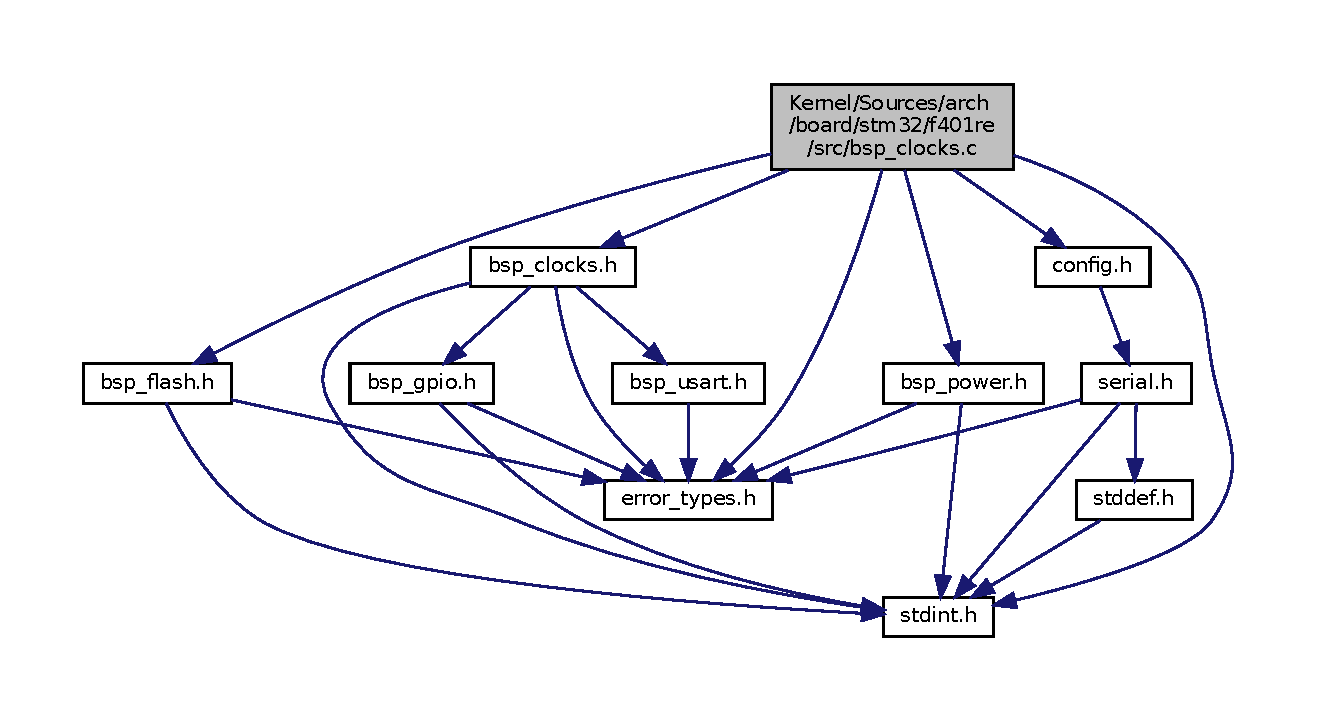
\includegraphics[width=350pt]{bsp__clocks_8c__incl}
\end{center}
\end{figure}
\subsection*{Functions}
\begin{DoxyCompactItemize}
\item 
void \hyperlink{bsp__clocks_8c_a0ce28d57a364aa3702778c54bb4d3c05}{bsp\+\_\+clk\+\_\+base\+\_\+sys\+\_\+init} (void)
\begin{DoxyCompactList}\small\item\em Initializes system clocks. \end{DoxyCompactList}\item 
void \hyperlink{bsp__clocks_8c_a1b855e007d20366749d59e4eda97222f}{bsp\+\_\+clk\+\_\+pll\+\_\+init} (void)
\begin{DoxyCompactList}\small\item\em Initializes system P\+LL clocks. \end{DoxyCompactList}\item 
void \hyperlink{bsp__clocks_8c_a69dea9163b1220130c719ac0b3b9327f}{bsp\+\_\+clk\+\_\+switch\+\_\+to\+\_\+pll} (void)
\begin{DoxyCompactList}\small\item\em Sets the system clock to be driven by P\+LL output. \end{DoxyCompactList}\item 
static \hyperlink{stdint_8h_a324c5d28c0d82f502a234ab99efac87a}{uint32\+\_\+t} \hyperlink{bsp__clocks_8c_ac154ab5d2a56dd8e09e0545e9775112e}{bsp\+\_\+clock\+\_\+get\+\_\+pll\+\_\+freq} (void)
\begin{DoxyCompactList}\small\item\em Get the P\+LL output frequency in M\+Hz. \end{DoxyCompactList}\item 
\hyperlink{error__types_8h_acf146bc98f60f47c79d782f7523e339c}{E\+R\+R\+O\+R\+\_\+\+C\+O\+D\+E\+\_\+E} \hyperlink{bsp__clocks_8c_a500b2e77b70c93b3f2b4a94cc9bcf79d}{bsp\+\_\+clk\+\_\+gpio\+\_\+enable} (const \hyperlink{bsp__gpio_8h_ab086506332275a2a873dfce02ed5a3b8}{G\+P\+I\+O\+\_\+\+I\+D\+E\+N\+T\+I\+F\+I\+E\+R\+\_\+E} gpio\+\_\+id)
\begin{DoxyCompactList}\small\item\em Enables the G\+P\+IO clocks. \end{DoxyCompactList}\item 
\hyperlink{error__types_8h_acf146bc98f60f47c79d782f7523e339c}{E\+R\+R\+O\+R\+\_\+\+C\+O\+D\+E\+\_\+E} \hyperlink{bsp__clocks_8c_aaf01af602e17579af5e6af009ae7a557}{bsp\+\_\+clk\+\_\+usart\+\_\+enable} (const \hyperlink{bsp__usart_8h_a594f9d90a9a3875660da4512fb208cf9}{U\+S\+A\+R\+T\+\_\+\+I\+D\+E\+N\+T\+I\+F\+I\+E\+R\+\_\+E} usart\+\_\+id)
\begin{DoxyCompactList}\small\item\em Enables the U\+S\+A\+RT clocks. \end{DoxyCompactList}\item 
\hyperlink{error__types_8h_acf146bc98f60f47c79d782f7523e339c}{E\+R\+R\+O\+R\+\_\+\+C\+O\+D\+E\+\_\+E} \hyperlink{bsp__clocks_8c_a286d003315af35aa9dd72b86ba6d8420}{bsp\+\_\+clk\+\_\+sys\+\_\+init} (void)
\begin{DoxyCompactList}\small\item\em Initializes system clocks. \end{DoxyCompactList}\item 
\hyperlink{stdint_8h_a324c5d28c0d82f502a234ab99efac87a}{uint32\+\_\+t} \hyperlink{bsp__clocks_8c_aeeded4b587684fa3383b3d42ee29af1e}{bsp\+\_\+clocks\+\_\+get\+\_\+freq} (const \hyperlink{bsp__clocks_8h_ac9d4d589a659370f313ef156f6eff0e8}{C\+L\+O\+C\+K\+\_\+\+I\+D\+E\+N\+T\+I\+F\+I\+E\+R\+\_\+T} clk\+\_\+id)
\begin{DoxyCompactList}\small\item\em Get the frequencies in M\+Hz of the clocks which identifer corresponds to the identifier given as parameter. \end{DoxyCompactList}\end{DoxyCompactItemize}
\subsection*{Variables}
\begin{DoxyCompactItemize}
\item 
static \hyperlink{stdint_8h_aba7bc1797add20fe3efdf37ced1182c5}{uint8\+\_\+t} \hyperlink{bsp__clocks_8c_a7e7b4728df96b76f3a8042b7fb46aa8c}{bsp\+\_\+clk\+\_\+init} = 0
\begin{DoxyCompactList}\small\item\em Stores the system clock init state. \end{DoxyCompactList}\item 
static const \hyperlink{stdint_8h_a273cf69d639a59973b6019625df33e30}{uint16\+\_\+t} \hyperlink{bsp__clocks_8c_abed7da9c2bfa6c8191c3bf928e64041f}{bsp\+\_\+hpre\+\_\+factor\+\_\+lookup} \mbox{[}8\mbox{]} = \{2, 4, 8, 16, 64, 128, 256, 512\}
\begin{DoxyCompactList}\small\item\em H\+R\+PE A\+HB prescaler factors lookup table. \end{DoxyCompactList}\item 
static const \hyperlink{stdint_8h_aba7bc1797add20fe3efdf37ced1182c5}{uint8\+\_\+t} \hyperlink{bsp__clocks_8c_a1ef2cd1399c95dbe65a524595da1fc5c}{bsp\+\_\+ppre\+\_\+factor\+\_\+lookup} \mbox{[}4\mbox{]} = \{2, 4, 8, 16\}
\begin{DoxyCompactList}\small\item\em P\+P\+RE prescaler factors lookup table. \end{DoxyCompactList}\end{DoxyCompactItemize}


\subsection{Function Documentation}
\mbox{\Hypertarget{bsp__clocks_8c_a0ce28d57a364aa3702778c54bb4d3c05}\label{bsp__clocks_8c_a0ce28d57a364aa3702778c54bb4d3c05}} 
\index{bsp\+\_\+clocks.\+c@{bsp\+\_\+clocks.\+c}!bsp\+\_\+clk\+\_\+base\+\_\+sys\+\_\+init@{bsp\+\_\+clk\+\_\+base\+\_\+sys\+\_\+init}}
\index{bsp\+\_\+clk\+\_\+base\+\_\+sys\+\_\+init@{bsp\+\_\+clk\+\_\+base\+\_\+sys\+\_\+init}!bsp\+\_\+clocks.\+c@{bsp\+\_\+clocks.\+c}}
\subsubsection{\texorpdfstring{bsp\+\_\+clk\+\_\+base\+\_\+sys\+\_\+init()}{bsp\_clk\_base\_sys\_init()}}
{\footnotesize\ttfamily void bsp\+\_\+clk\+\_\+base\+\_\+sys\+\_\+init (\begin{DoxyParamCaption}\item[{void}]{ }\end{DoxyParamCaption})}



Initializes system clocks. 

Initializes system clocks. The H\+SI is enabled and its calibration value. 

Definition at line 46 of file bsp\+\_\+clocks.\+c.


\begin{DoxyCode}
47 \{
48     *\hyperlink{bsp__clocks_8h_a2fcf7c04f16b1dd27c577a9a14c5ff96}{RCC\_CR\_REGISTER} = (*\hyperlink{bsp__clocks_8h_a2fcf7c04f16b1dd27c577a9a14c5ff96}{RCC\_CR\_REGISTER} & ~
      \hyperlink{bsp__clocks_8h_a73f9913edb8b30eb2b8aa1b5d29b297e}{RCC\_CR\_HSITRIM\_MASK}) | 
49                        (\hyperlink{bsp__clocks_8h_af4fcacf94a97f7d49a70e089b39cf474}{RCC\_CR\_HSION} | \hyperlink{bsp__clocks_8h_a12241a92893b4023a40e85d3b371ac05}{RCC\_CR\_HSITRIM\_DEF});
50     \textcolor{keywordflow}{while}((*\hyperlink{bsp__clocks_8h_a2fcf7c04f16b1dd27c577a9a14c5ff96}{RCC\_CR\_REGISTER} & \hyperlink{bsp__clocks_8h_a9dbac3f2bc04f04ebafe1e66ae3fcf0d}{RCC\_CR\_HSIRDY}) == 0);
51 \}
\end{DoxyCode}
Here is the caller graph for this function\+:\nopagebreak
\begin{figure}[H]
\begin{center}
\leavevmode
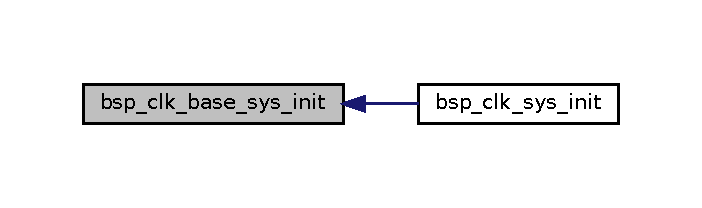
\includegraphics[width=337pt]{bsp__clocks_8c_a0ce28d57a364aa3702778c54bb4d3c05_icgraph}
\end{center}
\end{figure}
\mbox{\Hypertarget{bsp__clocks_8c_a500b2e77b70c93b3f2b4a94cc9bcf79d}\label{bsp__clocks_8c_a500b2e77b70c93b3f2b4a94cc9bcf79d}} 
\index{bsp\+\_\+clocks.\+c@{bsp\+\_\+clocks.\+c}!bsp\+\_\+clk\+\_\+gpio\+\_\+enable@{bsp\+\_\+clk\+\_\+gpio\+\_\+enable}}
\index{bsp\+\_\+clk\+\_\+gpio\+\_\+enable@{bsp\+\_\+clk\+\_\+gpio\+\_\+enable}!bsp\+\_\+clocks.\+c@{bsp\+\_\+clocks.\+c}}
\subsubsection{\texorpdfstring{bsp\+\_\+clk\+\_\+gpio\+\_\+enable()}{bsp\_clk\_gpio\_enable()}}
{\footnotesize\ttfamily \hyperlink{error__types_8h_acf146bc98f60f47c79d782f7523e339c}{E\+R\+R\+O\+R\+\_\+\+C\+O\+D\+E\+\_\+E} bsp\+\_\+clk\+\_\+gpio\+\_\+enable (\begin{DoxyParamCaption}\item[{const \hyperlink{bsp__gpio_8h_ab086506332275a2a873dfce02ed5a3b8}{G\+P\+I\+O\+\_\+\+I\+D\+E\+N\+T\+I\+F\+I\+E\+R\+\_\+E}}]{gpio\+\_\+id }\end{DoxyParamCaption})}



Enables the G\+P\+IO clocks. 

Enables the G\+P\+IO clocks. This function will enable the peripheral clock used by the G\+P\+IO corresponding to the identifier given as parameter. If the identifier is unknown, the function has no effect.


\begin{DoxyParams}[1]{Parameters}
\mbox{\tt in}  & {\em gpio\+\_\+id} & The G\+P\+IO identifier for which the clock should be enabled.\\
\hline
\end{DoxyParams}
\begin{DoxyReturn}{Returns}
N\+O\+\_\+\+E\+R\+R\+OR is returned in case of success. Otherwise an error code is returned. Please refer to the list of the standard error codes. 
\end{DoxyReturn}


Definition at line 145 of file bsp\+\_\+clocks.\+c.


\begin{DoxyCode}
146 \{
147     \hyperlink{stdint_8h_a324c5d28c0d82f502a234ab99efac87a}{uint32\_t} reg\_val;
148 
149     \textcolor{keywordflow}{switch}(gpio\_id)
150     \{
151         \textcolor{keywordflow}{case} \hyperlink{bsp__gpio_8h_a69f521b579d2c761dd65949f2bae88f3a4cb73b98ec508807d984052a1598950a}{GPIO\_ID\_A}:
152             reg\_val = \hyperlink{bsp__clocks_8h_a6ff46fb3b30fc6792e4fd18fcb0941b5}{RCC\_AHB1ENR\_GPIOAEN};
153             \textcolor{keywordflow}{break};
154         \textcolor{keywordflow}{case} \hyperlink{bsp__gpio_8h_a69f521b579d2c761dd65949f2bae88f3a9fc59b324d277c00de32d87f8072b56a}{GPIO\_ID\_B}:
155             reg\_val = \hyperlink{bsp__clocks_8h_ad7f408f92e7fd49b0957b8cb4ff31ca5}{RCC\_AHB1ENR\_GPIOBEN};
156             \textcolor{keywordflow}{break};
157         \textcolor{keywordflow}{case} \hyperlink{bsp__gpio_8h_a69f521b579d2c761dd65949f2bae88f3afae76fa0a334173cbea6472ae010d0a9}{GPIO\_ID\_C}:
158             reg\_val = \hyperlink{bsp__clocks_8h_ae8a8b42e33aef2a7bc2d41ad9d231733}{RCC\_AHB1ENR\_GPIOCEN};
159             \textcolor{keywordflow}{break};
160         \textcolor{keywordflow}{case} \hyperlink{bsp__gpio_8h_a69f521b579d2c761dd65949f2bae88f3ad6df84175b0fc74ef3c655082b648918}{GPIO\_ID\_D}:
161             reg\_val = \hyperlink{bsp__clocks_8h_aebd8146e91c76f14af8dfe78a1c2d916}{RCC\_AHB1ENR\_GPIODEN};
162             \textcolor{keywordflow}{break};
163         \textcolor{keywordflow}{case} \hyperlink{bsp__gpio_8h_a69f521b579d2c761dd65949f2bae88f3a496fabc0d5663f4956df5e9a4d275ed4}{GPIO\_ID\_E}:
164             reg\_val = \hyperlink{bsp__clocks_8h_a67a9094e0e464eaa8e25f854f90abfc6}{RCC\_AHB1ENR\_GPIOEEN};
165             \textcolor{keywordflow}{break};
166         \textcolor{keywordflow}{case} \hyperlink{bsp__gpio_8h_a69f521b579d2c761dd65949f2bae88f3aa25ae326f6c8e013c190052d0a3c7d29}{GPIO\_ID\_H}:
167             reg\_val = \hyperlink{bsp__clocks_8h_adb16afc550121895822ebb22108196b6}{RCC\_AHB1ENR\_GPIOHEN};
168             \textcolor{keywordflow}{break};
169         \textcolor{keywordflow}{default}:
170             reg\_val = 0;
171     \}
172 
173     \textcolor{keywordflow}{if}(reg\_val == 0)
174     \{
175 \textcolor{preprocessor}{#if KERNEL\_LOG\_LEVEL == ERROR\_LOG\_LEVEL
}
176         \hyperlink{logger_8h_a580bb63c1418b2fc8456f9b6c5b6d39d}{KERNEL\_LOG\_ERROR}(\textcolor{stringliteral}{"Wrong GPIO identifer"}, 
177                          gpio\_id, 
178                          \textcolor{keyword}{sizeof}(gpio\_id), 
179                          \hyperlink{error__types_8h_a4db9ee29f2ff83c71567c12f6bfbf28cabbe6797281350f36c23d07d6f2d7f6e2}{ERROR\_INVALID\_PARAM});
180 \textcolor{preprocessor}{#endif
}
181         \textcolor{keywordflow}{return} \hyperlink{error__types_8h_a4db9ee29f2ff83c71567c12f6bfbf28cabbe6797281350f36c23d07d6f2d7f6e2}{ERROR\_INVALID\_PARAM};
182     \}
183 
184     *\hyperlink{bsp__clocks_8h_a4c6aae1c96c5acee8a320c6b2a8aaee5}{RCC\_AHB1ENR\_REGISTER} = *\hyperlink{bsp__clocks_8h_a4c6aae1c96c5acee8a320c6b2a8aaee5}{RCC\_AHB1ENR\_REGISTER} | reg\_val;
185     \textcolor{keywordflow}{while}((*\hyperlink{bsp__clocks_8h_a4c6aae1c96c5acee8a320c6b2a8aaee5}{RCC\_AHB1ENR\_REGISTER} & reg\_val) == 0);
186 
187 \textcolor{preprocessor}{#if KERNEL\_LOG\_LEVEL >= INFO\_LOG\_LEVEL
}
188         KERNEL\_LOG\_INFO(\textcolor{stringliteral}{"GPIO clock enabled"}, 
189                         gpio\_id, 
190                         \textcolor{keyword}{sizeof}(gpio\_id), 
191                         \hyperlink{error__types_8h_a4db9ee29f2ff83c71567c12f6bfbf28cabf350750d0d4fabd8954c0f1e9bbae94}{NO\_ERROR});
192 \textcolor{preprocessor}{#endif
}
193 
194     \textcolor{keywordflow}{return} \hyperlink{error__types_8h_a4db9ee29f2ff83c71567c12f6bfbf28cabf350750d0d4fabd8954c0f1e9bbae94}{NO\_ERROR};
195 \}
\end{DoxyCode}
Here is the call graph for this function\+:\nopagebreak
\begin{figure}[H]
\begin{center}
\leavevmode
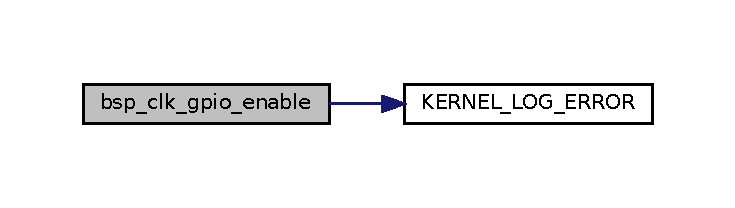
\includegraphics[width=350pt]{bsp__clocks_8c_a500b2e77b70c93b3f2b4a94cc9bcf79d_cgraph}
\end{center}
\end{figure}
Here is the caller graph for this function\+:\nopagebreak
\begin{figure}[H]
\begin{center}
\leavevmode
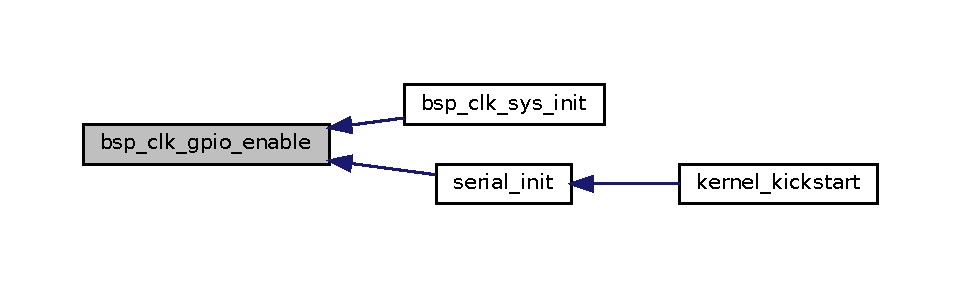
\includegraphics[width=350pt]{bsp__clocks_8c_a500b2e77b70c93b3f2b4a94cc9bcf79d_icgraph}
\end{center}
\end{figure}
\mbox{\Hypertarget{bsp__clocks_8c_a1b855e007d20366749d59e4eda97222f}\label{bsp__clocks_8c_a1b855e007d20366749d59e4eda97222f}} 
\index{bsp\+\_\+clocks.\+c@{bsp\+\_\+clocks.\+c}!bsp\+\_\+clk\+\_\+pll\+\_\+init@{bsp\+\_\+clk\+\_\+pll\+\_\+init}}
\index{bsp\+\_\+clk\+\_\+pll\+\_\+init@{bsp\+\_\+clk\+\_\+pll\+\_\+init}!bsp\+\_\+clocks.\+c@{bsp\+\_\+clocks.\+c}}
\subsubsection{\texorpdfstring{bsp\+\_\+clk\+\_\+pll\+\_\+init()}{bsp\_clk\_pll\_init()}}
{\footnotesize\ttfamily void bsp\+\_\+clk\+\_\+pll\+\_\+init (\begin{DoxyParamCaption}\item[{void}]{ }\end{DoxyParamCaption})}



Initializes system P\+LL clocks. 

Initializes system P\+LL clocks. The P\+LL are set for a system clock of 84\+M\+Hz and bus to 48\+M\+Hz. 

Definition at line 59 of file bsp\+\_\+clocks.\+c.


\begin{DoxyCode}
60 \{
61     \textcolor{comment}{/* PLL should be disabled at that point */}
62     *\hyperlink{bsp__clocks_8h_ad2d60b66a5292f1c04c7c3ebfe9df335}{RCC\_PLLCFGR\_REGISTER} = *\hyperlink{bsp__clocks_8h_ad2d60b66a5292f1c04c7c3ebfe9df335}{RCC\_PLLCFGR\_REGISTER} & 
63                             ~(\hyperlink{bsp__clocks_8h_afaac3bc429eaa475ca5e431a020d4c67}{RCC\_PLLCFGR\_PLLM\_MASK} | 
      \hyperlink{bsp__clocks_8h_a90997335764397eb4be02c23676cda4a}{RCC\_PLLCFGR\_PLLN\_MASK} | 
64                               \hyperlink{bsp__clocks_8h_a40a7c5938dfdd0ab63dcf3b203da7dd4}{RCC\_PLLCFGR\_PLLP\_MASK} | 
      \hyperlink{bsp__clocks_8h_ad4784939ce13e81f2cc64dda2b5d8770}{RCC\_PLLCFGR\_PLLQ\_MASK} | 
65                               \hyperlink{bsp__clocks_8h_a6c5c6a2e8d760ad7da85ae2c8076ee31}{RCC\_PLLCFGR\_PLLSRC\_MASK});
66 
67     \textcolor{comment}{/* Set the PLL values */}
68     *\hyperlink{bsp__clocks_8h_ad2d60b66a5292f1c04c7c3ebfe9df335}{RCC\_PLLCFGR\_REGISTER} = *\hyperlink{bsp__clocks_8h_ad2d60b66a5292f1c04c7c3ebfe9df335}{RCC\_PLLCFGR\_REGISTER} |
69                             (\hyperlink{bsp__clocks_8h_adc4eb2ce50286dc96d4976b9689be1d7}{RCC\_PLLM\_VALUE} << 
      \hyperlink{bsp__clocks_8h_add5fc49687031bdd44fca9c909f74fe0}{RCC\_PLLCFGR\_PLLM\_OFFSET}) |
70                             (\hyperlink{bsp__clocks_8h_a11fa93ae89931a632e06eb0694ff62b7}{RCC\_PLLN\_VALUE} << 
      \hyperlink{bsp__clocks_8h_adc0f70732fb3d933c96d741f27baec35}{RCC\_PLLCFGR\_PLLN\_OFFSET}) |
71                             (\hyperlink{bsp__clocks_8h_a9ad812030f6e208e79df8e9bddb96c19}{RCC\_PLLP\_VALUE} << 
      \hyperlink{bsp__clocks_8h_a9a6c6234e6c59e7638d1a8edd237f591}{RCC\_PLLCFGR\_PLLP\_OFFSET}) |
72                             (\hyperlink{bsp__clocks_8h_a0babc931753727d1ee6b56d41a51f598}{RCC\_PLLQ\_VALUE} << 
      \hyperlink{bsp__clocks_8h_aa47b1576488cea5e741f58cce74337c9}{RCC\_PLLCFGR\_PLLQ\_OFFSET}) |
73                             (\hyperlink{bsp__clocks_8h_ae90c3d400891ac3355363979581bd924}{RCC\_PLLSRC\_VALUE} << 
      \hyperlink{bsp__clocks_8h_a001728588571f89b2b52e6a903e66395}{RCC\_PLLCFGR\_PLLSRC\_OFFSET});
74 
75     \textcolor{comment}{/* Enable PLLs */}
76     *\hyperlink{bsp__clocks_8h_a2fcf7c04f16b1dd27c577a9a14c5ff96}{RCC\_CR\_REGISTER} = *\hyperlink{bsp__clocks_8h_a2fcf7c04f16b1dd27c577a9a14c5ff96}{RCC\_CR\_REGISTER} | 
      \hyperlink{bsp__clocks_8h_ad0e73d5b0a4883e074d40029b49ee47e}{RCC\_CR\_PLLON};
77     
78     \textcolor{comment}{/* Wait for PLL lock */}
79     \textcolor{keywordflow}{while}((*\hyperlink{bsp__clocks_8h_a2fcf7c04f16b1dd27c577a9a14c5ff96}{RCC\_CR\_REGISTER} & \hyperlink{bsp__clocks_8h_afa12d7ac6a7f0f91d066aeb2c6071888}{RCC\_CR\_PLLRDY}) == 0);
80 \}
\end{DoxyCode}
Here is the caller graph for this function\+:\nopagebreak
\begin{figure}[H]
\begin{center}
\leavevmode
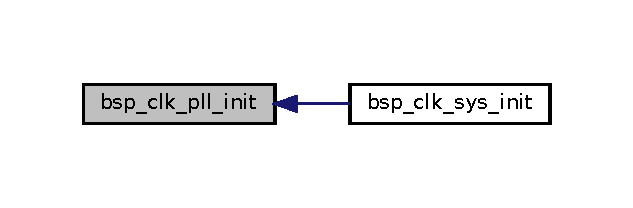
\includegraphics[width=304pt]{bsp__clocks_8c_a1b855e007d20366749d59e4eda97222f_icgraph}
\end{center}
\end{figure}
\mbox{\Hypertarget{bsp__clocks_8c_a69dea9163b1220130c719ac0b3b9327f}\label{bsp__clocks_8c_a69dea9163b1220130c719ac0b3b9327f}} 
\index{bsp\+\_\+clocks.\+c@{bsp\+\_\+clocks.\+c}!bsp\+\_\+clk\+\_\+switch\+\_\+to\+\_\+pll@{bsp\+\_\+clk\+\_\+switch\+\_\+to\+\_\+pll}}
\index{bsp\+\_\+clk\+\_\+switch\+\_\+to\+\_\+pll@{bsp\+\_\+clk\+\_\+switch\+\_\+to\+\_\+pll}!bsp\+\_\+clocks.\+c@{bsp\+\_\+clocks.\+c}}
\subsubsection{\texorpdfstring{bsp\+\_\+clk\+\_\+switch\+\_\+to\+\_\+pll()}{bsp\_clk\_switch\_to\_pll()}}
{\footnotesize\ttfamily void bsp\+\_\+clk\+\_\+switch\+\_\+to\+\_\+pll (\begin{DoxyParamCaption}\item[{void}]{ }\end{DoxyParamCaption})}



Sets the system clock to be driven by P\+LL output. 

Sets the system clock to be driven by P\+LL output. 

Definition at line 87 of file bsp\+\_\+clocks.\+c.


\begin{DoxyCode}
88 \{
89     \textcolor{comment}{/* Set AHB, APB1 and APB2 prescaler values */}
90     *\hyperlink{bsp__clocks_8h_ac454715dd9c4f8ba957cc53f318c58ac}{RCC\_CFGR\_REGISTER} = *\hyperlink{bsp__clocks_8h_ac454715dd9c4f8ba957cc53f318c58ac}{RCC\_CFGR\_REGISTER} & 
91                         ~(\hyperlink{bsp__clocks_8h_a7b024c33f9bd185d923b55af2360fec5}{RCC\_CFGR\_HRPE\_MASK}  |
92                           \hyperlink{bsp__clocks_8h_a1220a63e00de9ff4a2a45474ead3662d}{RCC\_CFGR\_PPRE1\_MASK} |
93                           \hyperlink{bsp__clocks_8h_a41aef118b0611444caa87df8ea302dc2}{RCC\_CFGR\_PPRE2\_MASK});
94     *\hyperlink{bsp__clocks_8h_ac454715dd9c4f8ba957cc53f318c58ac}{RCC\_CFGR\_REGISTER} = *\hyperlink{bsp__clocks_8h_ac454715dd9c4f8ba957cc53f318c58ac}{RCC\_CFGR\_REGISTER}   | 
      \hyperlink{bsp__clocks_8h_a3fe59bf63a37a12304f37d7babec3eeb}{RCC\_CFGR\_HRPE\_DIV1} | 
95                           \hyperlink{bsp__clocks_8h_af832ad6844c907d9bb37c1536defcb0d}{RCC\_CFGR\_PPRE1\_DIV2} | 
      \hyperlink{bsp__clocks_8h_a247aebf1999a38ea07785558d277bb1a}{RCC\_CFGR\_PPRE2\_DIV1};
96 
97     \textcolor{comment}{/* Set the system clock to use PLL as input */}
98     *\hyperlink{bsp__clocks_8h_ac454715dd9c4f8ba957cc53f318c58ac}{RCC\_CFGR\_REGISTER} = (*\hyperlink{bsp__clocks_8h_ac454715dd9c4f8ba957cc53f318c58ac}{RCC\_CFGR\_REGISTER} & ~
      \hyperlink{bsp__clocks_8h_a7e5e28699fe923870e15fef3651ff3ef}{RCC\_CFGR\_SW\_MASK}) | 
99                         \hyperlink{bsp__clocks_8h_a87389cacb2eaf53730da13a2a33cd487}{RCC\_CFGR\_SW\_PLL};
100     
101     \textcolor{comment}{/* Wait for update */}
102     \textcolor{keywordflow}{while}((*\hyperlink{bsp__clocks_8h_ac454715dd9c4f8ba957cc53f318c58ac}{RCC\_CFGR\_REGISTER} & \hyperlink{bsp__clocks_8h_a451045d952eb1caaa0090c9e8dc75082}{RCC\_CFGR\_SWS\_MASK}) != 
      \hyperlink{bsp__clocks_8h_a2c67e2279804a83ef24438267d9d4a6c}{RCC\_CFGR\_SWS\_PLL});
103 \}
\end{DoxyCode}
Here is the caller graph for this function\+:\nopagebreak
\begin{figure}[H]
\begin{center}
\leavevmode
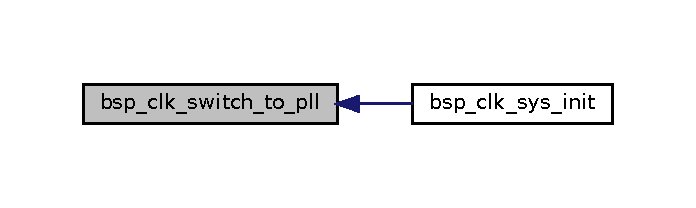
\includegraphics[width=334pt]{bsp__clocks_8c_a69dea9163b1220130c719ac0b3b9327f_icgraph}
\end{center}
\end{figure}
\mbox{\Hypertarget{bsp__clocks_8c_a286d003315af35aa9dd72b86ba6d8420}\label{bsp__clocks_8c_a286d003315af35aa9dd72b86ba6d8420}} 
\index{bsp\+\_\+clocks.\+c@{bsp\+\_\+clocks.\+c}!bsp\+\_\+clk\+\_\+sys\+\_\+init@{bsp\+\_\+clk\+\_\+sys\+\_\+init}}
\index{bsp\+\_\+clk\+\_\+sys\+\_\+init@{bsp\+\_\+clk\+\_\+sys\+\_\+init}!bsp\+\_\+clocks.\+c@{bsp\+\_\+clocks.\+c}}
\subsubsection{\texorpdfstring{bsp\+\_\+clk\+\_\+sys\+\_\+init()}{bsp\_clk\_sys\_init()}}
{\footnotesize\ttfamily \hyperlink{error__types_8h_acf146bc98f60f47c79d782f7523e339c}{E\+R\+R\+O\+R\+\_\+\+C\+O\+D\+E\+\_\+E} bsp\+\_\+clk\+\_\+sys\+\_\+init (\begin{DoxyParamCaption}\item[{void}]{ }\end{DoxyParamCaption})}



Initializes system clocks. 

Initializes system clocks. The C\+PU, A\+HB and A\+PB clocks are initialized. The function also sets the regulator output voltage needed by the clocks.

\begin{DoxyReturn}{Returns}
N\+O\+\_\+\+E\+R\+R\+OR is returned in case of success. Otherwise an error code is returned. Please refer to the list of the standard error codes. 
\end{DoxyReturn}


Definition at line 242 of file bsp\+\_\+clocks.\+c.


\begin{DoxyCode}
243 \{
244     \hyperlink{error__types_8h_acf146bc98f60f47c79d782f7523e339c}{ERROR\_CODE\_E} error;
245 
246     \textcolor{comment}{/* Check init state */}
247     \textcolor{keywordflow}{if}(\hyperlink{bsp__clocks_8c_a7e7b4728df96b76f3a8042b7fb46aa8c}{bsp\_clk\_init} != 0)
248     \{
249 \textcolor{preprocessor}{#if KERNEL\_LOG\_LEVEL == ERROR\_LOG\_LEVEL
}
250         \hyperlink{logger_8h_a580bb63c1418b2fc8456f9b6c5b6d39d}{KERNEL\_LOG\_ERROR}(\textcolor{stringliteral}{"System clock is already initialized"}, 
251                          \hyperlink{error__types_8h_a4db9ee29f2ff83c71567c12f6bfbf28ca9af911a6ba1c32ce22213d689cb59f86}{ERROR\_ALREADY\_INIT}, 
252                          \textcolor{keyword}{sizeof}(\hyperlink{error__types_8h_a4db9ee29f2ff83c71567c12f6bfbf28ca9af911a6ba1c32ce22213d689cb59f86}{ERROR\_ALREADY\_INIT}), 
253                          \hyperlink{error__types_8h_a4db9ee29f2ff83c71567c12f6bfbf28ca9af911a6ba1c32ce22213d689cb59f86}{ERROR\_ALREADY\_INIT});
254 \textcolor{preprocessor}{#endif
}
255         \textcolor{keywordflow}{return} \hyperlink{error__types_8h_a4db9ee29f2ff83c71567c12f6bfbf28ca9af911a6ba1c32ce22213d689cb59f86}{ERROR\_ALREADY\_INIT};
256     \}
257 
258     \textcolor{comment}{/* Enable the power interface clock and system clock controller */}
259     *\hyperlink{bsp__clocks_8h_aae3fa9b2133a67e3ca65db35f8ac9a4c}{RCC\_APB1ENR\_REGISTER} = *\hyperlink{bsp__clocks_8h_aae3fa9b2133a67e3ca65db35f8ac9a4c}{RCC\_APB1ENR\_REGISTER} | 
      \hyperlink{bsp__clocks_8h_a5c19997ccd28464b80a7c3325da0ca60}{RCC\_APB1ENR\_PWREN};
260     \textcolor{keywordflow}{while}((*\hyperlink{bsp__clocks_8h_aae3fa9b2133a67e3ca65db35f8ac9a4c}{RCC\_APB1ENR\_REGISTER} & \hyperlink{bsp__clocks_8h_a5c19997ccd28464b80a7c3325da0ca60}{RCC\_APB1ENR\_PWREN}) == 0);
261     *\hyperlink{bsp__clocks_8h_aae721f66e88c2e4264580d95d5ffdd59}{RCC\_APB2ENR\_REGISTER} = *\hyperlink{bsp__clocks_8h_aae721f66e88c2e4264580d95d5ffdd59}{RCC\_APB2ENR\_REGISTER} | 
      \hyperlink{bsp__clocks_8h_a7a9d56a8aa1fa0f519ecbdf0d19dd4da}{RCC\_APB2ENR\_SYSCFGEN};
262     \textcolor{keywordflow}{while}((*\hyperlink{bsp__clocks_8h_aae721f66e88c2e4264580d95d5ffdd59}{RCC\_APB2ENR\_REGISTER} & \hyperlink{bsp__clocks_8h_a7a9d56a8aa1fa0f519ecbdf0d19dd4da}{RCC\_APB2ENR\_SYSCFGEN}) == 0);
263 
264     \textcolor{comment}{/* Update voltage scaling */}
265     error = \hyperlink{bsp__power_8h_abe4bd68d683c1ab3fbc83afb60b36ede}{bsp\_pwr\_set\_scaling}(\hyperlink{bsp__power_8h_aeab31582495468040935b45b76f06553a8ddc2bb242e2a77509aad0d808c22339}{POWER\_SCALING\_MODE\_2});
266     \textcolor{keywordflow}{if}(error != \hyperlink{error__types_8h_a4db9ee29f2ff83c71567c12f6bfbf28cabf350750d0d4fabd8954c0f1e9bbae94}{NO\_ERROR})
267     \{
268         \textcolor{keywordflow}{return} error;
269     \}
270     
271     \textcolor{comment}{/* Set flash latency */}
272     error = \hyperlink{bsp__flash_8h_a51f3c79743adab8e26ca7a5c6b33c55b}{bsp\_flash\_set\_latency}(\hyperlink{bsp__flash_8h_ad230debff3c818a6f9ced62364bc86c0ad84e36d61f83d1f0104cb3384726476c}{FLASH\_LATENCY\_WS\_2});
273     \textcolor{keywordflow}{if}(error != \hyperlink{error__types_8h_a4db9ee29f2ff83c71567c12f6bfbf28cabf350750d0d4fabd8954c0f1e9bbae94}{NO\_ERROR})
274     \{
275         \textcolor{keywordflow}{return} error;
276     \}
277 
278     \textcolor{comment}{/* Init systems clocks */}
279     \hyperlink{bsp__clocks_8c_a0ce28d57a364aa3702778c54bb4d3c05}{bsp\_clk\_base\_sys\_init}();
280     \hyperlink{bsp__clocks_8c_a1b855e007d20366749d59e4eda97222f}{bsp\_clk\_pll\_init}();
281     \hyperlink{bsp__clocks_8c_a69dea9163b1220130c719ac0b3b9327f}{bsp\_clk\_switch\_to\_pll}();
282 
283     \textcolor{comment}{/* Init GPIO and USART clocks */}
284     error = \hyperlink{bsp__clocks_8c_a500b2e77b70c93b3f2b4a94cc9bcf79d}{bsp\_clk\_gpio\_enable}(\hyperlink{bsp__gpio_8h_a69f521b579d2c761dd65949f2bae88f3a4cb73b98ec508807d984052a1598950a}{GPIO\_ID\_A});
285     \textcolor{keywordflow}{if}(error != \hyperlink{error__types_8h_a4db9ee29f2ff83c71567c12f6bfbf28cabf350750d0d4fabd8954c0f1e9bbae94}{NO\_ERROR})
286     \{
287         \textcolor{keywordflow}{return} error;
288     \}
289     error = \hyperlink{bsp__clocks_8c_aaf01af602e17579af5e6af009ae7a557}{bsp\_clk\_usart\_enable}(\hyperlink{bsp__usart_8h_a58f9be3820e29e0fbf00e2466c3ee768abb138542d801249fd01ec62c34f52cff}{USART\_ID\_2});
290     \textcolor{keywordflow}{if}(error != \hyperlink{error__types_8h_a4db9ee29f2ff83c71567c12f6bfbf28cabf350750d0d4fabd8954c0f1e9bbae94}{NO\_ERROR})
291     \{
292         \textcolor{keywordflow}{return} error;
293     \}
294 
295 \textcolor{preprocessor}{#if KERNEL\_LOG\_LEVEL >= INFO\_LOG\_LEVEL
}
296     KERNEL\_LOG\_INFO(\textcolor{stringliteral}{"System clock initialized"}, 
297                     \hyperlink{error__types_8h_a4db9ee29f2ff83c71567c12f6bfbf28cabf350750d0d4fabd8954c0f1e9bbae94}{NO\_ERROR}, 
298                     \textcolor{keyword}{sizeof}(\hyperlink{error__types_8h_a4db9ee29f2ff83c71567c12f6bfbf28cabf350750d0d4fabd8954c0f1e9bbae94}{NO\_ERROR}), 
299                     \hyperlink{error__types_8h_a4db9ee29f2ff83c71567c12f6bfbf28cabf350750d0d4fabd8954c0f1e9bbae94}{NO\_ERROR});
300 \textcolor{preprocessor}{#endif
}
301 
302     \textcolor{comment}{/* Update init state */}
303     \hyperlink{bsp__clocks_8c_a7e7b4728df96b76f3a8042b7fb46aa8c}{bsp\_clk\_init} = 1;
304     \textcolor{keywordflow}{return} \hyperlink{error__types_8h_a4db9ee29f2ff83c71567c12f6bfbf28cabf350750d0d4fabd8954c0f1e9bbae94}{NO\_ERROR};
305 \}
\end{DoxyCode}
Here is the call graph for this function\+:\nopagebreak
\begin{figure}[H]
\begin{center}
\leavevmode
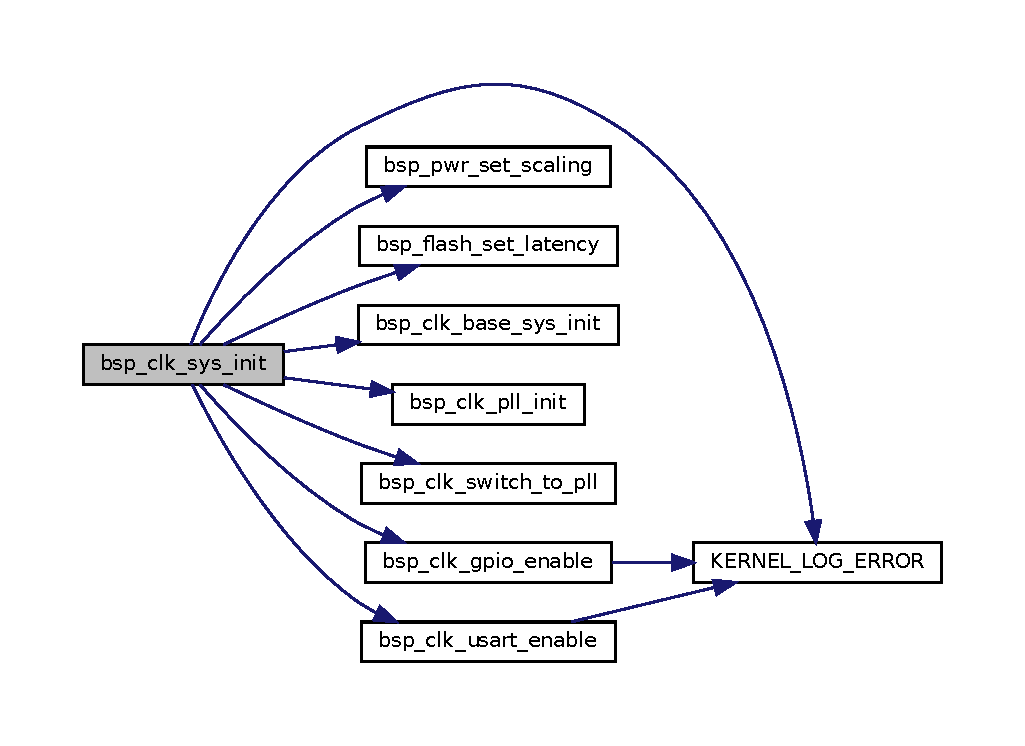
\includegraphics[width=350pt]{bsp__clocks_8c_a286d003315af35aa9dd72b86ba6d8420_cgraph}
\end{center}
\end{figure}
\mbox{\Hypertarget{bsp__clocks_8c_aaf01af602e17579af5e6af009ae7a557}\label{bsp__clocks_8c_aaf01af602e17579af5e6af009ae7a557}} 
\index{bsp\+\_\+clocks.\+c@{bsp\+\_\+clocks.\+c}!bsp\+\_\+clk\+\_\+usart\+\_\+enable@{bsp\+\_\+clk\+\_\+usart\+\_\+enable}}
\index{bsp\+\_\+clk\+\_\+usart\+\_\+enable@{bsp\+\_\+clk\+\_\+usart\+\_\+enable}!bsp\+\_\+clocks.\+c@{bsp\+\_\+clocks.\+c}}
\subsubsection{\texorpdfstring{bsp\+\_\+clk\+\_\+usart\+\_\+enable()}{bsp\_clk\_usart\_enable()}}
{\footnotesize\ttfamily \hyperlink{error__types_8h_acf146bc98f60f47c79d782f7523e339c}{E\+R\+R\+O\+R\+\_\+\+C\+O\+D\+E\+\_\+E} bsp\+\_\+clk\+\_\+usart\+\_\+enable (\begin{DoxyParamCaption}\item[{const \hyperlink{bsp__usart_8h_a594f9d90a9a3875660da4512fb208cf9}{U\+S\+A\+R\+T\+\_\+\+I\+D\+E\+N\+T\+I\+F\+I\+E\+R\+\_\+E}}]{usart\+\_\+id }\end{DoxyParamCaption})}



Enables the U\+S\+A\+RT clocks. 

Enables the U\+S\+A\+RT clocks. This function will enable the peripheral clock used by the U\+S\+A\+RT corresponding to the identifier given as parameter. If the identifier is unknown, the function has no effect.


\begin{DoxyParams}[1]{Parameters}
\mbox{\tt in}  & {\em usart\+\_\+id} & The U\+S\+A\+RT identifier for which the clock should be enabled.\\
\hline
\end{DoxyParams}
\begin{DoxyReturn}{Returns}
N\+O\+\_\+\+E\+R\+R\+OR is returned in case of success. Otherwise an error code is returned. Please refer to the list of the standard error codes. 
\end{DoxyReturn}


Definition at line 197 of file bsp\+\_\+clocks.\+c.


\begin{DoxyCode}
198 \{
199     \hyperlink{error__types_8h_acf146bc98f60f47c79d782f7523e339c}{ERROR\_CODE\_E} error;
200 
201     error = \hyperlink{error__types_8h_a4db9ee29f2ff83c71567c12f6bfbf28cabf350750d0d4fabd8954c0f1e9bbae94}{NO\_ERROR};
202 
203     \textcolor{comment}{/* Select the USART interface */}
204     \textcolor{keywordflow}{switch}(usart\_id)
205     \{
206         \textcolor{keywordflow}{case} \hyperlink{bsp__usart_8h_a58f9be3820e29e0fbf00e2466c3ee768a512d550c862eac9ad45d923508bb0f7d}{USART\_ID\_1}:
207             *\hyperlink{bsp__clocks_8h_aae721f66e88c2e4264580d95d5ffdd59}{RCC\_APB2ENR\_REGISTER} = *\hyperlink{bsp__clocks_8h_aae721f66e88c2e4264580d95d5ffdd59}{RCC\_APB2ENR\_REGISTER} | 
208                                      \hyperlink{bsp__clocks_8h_a4666bb90842e8134b32e6a34a0f165f3}{RCC\_APB2ENR\_USART1EN};
209             \textcolor{keywordflow}{while}((*\hyperlink{bsp__clocks_8h_aae721f66e88c2e4264580d95d5ffdd59}{RCC\_APB2ENR\_REGISTER} & 
      \hyperlink{bsp__clocks_8h_a4666bb90842e8134b32e6a34a0f165f3}{RCC\_APB2ENR\_USART1EN}) == 0);
210             \textcolor{keywordflow}{break};
211         \textcolor{keywordflow}{case} \hyperlink{bsp__usart_8h_a58f9be3820e29e0fbf00e2466c3ee768abb138542d801249fd01ec62c34f52cff}{USART\_ID\_2}:
212             *\hyperlink{bsp__clocks_8h_aae3fa9b2133a67e3ca65db35f8ac9a4c}{RCC\_APB1ENR\_REGISTER} = *\hyperlink{bsp__clocks_8h_aae3fa9b2133a67e3ca65db35f8ac9a4c}{RCC\_APB1ENR\_REGISTER} | 
213                                      \hyperlink{bsp__clocks_8h_ab840af4f735ec36419d61c7db3cfa00d}{RCC\_APB1ENR\_USART2EN};
214             \textcolor{keywordflow}{while}((*\hyperlink{bsp__clocks_8h_aae3fa9b2133a67e3ca65db35f8ac9a4c}{RCC\_APB1ENR\_REGISTER} & 
      \hyperlink{bsp__clocks_8h_ab840af4f735ec36419d61c7db3cfa00d}{RCC\_APB1ENR\_USART2EN}) == 0);
215             \textcolor{keywordflow}{break};
216         \textcolor{keywordflow}{case} \hyperlink{bsp__usart_8h_a58f9be3820e29e0fbf00e2466c3ee768afd45e5de3678cbcada70f46bde327479}{USART\_ID\_6}:
217             *\hyperlink{bsp__clocks_8h_aae721f66e88c2e4264580d95d5ffdd59}{RCC\_APB2ENR\_REGISTER} = *\hyperlink{bsp__clocks_8h_aae721f66e88c2e4264580d95d5ffdd59}{RCC\_APB2ENR\_REGISTER} | 
218                                      \hyperlink{bsp__clocks_8h_a0569d91f3b18ae130b7a09e0100c4459}{RCC\_APB2ENR\_USART6EN};
219             \textcolor{keywordflow}{while}((*\hyperlink{bsp__clocks_8h_aae721f66e88c2e4264580d95d5ffdd59}{RCC\_APB2ENR\_REGISTER} & 
      \hyperlink{bsp__clocks_8h_a0569d91f3b18ae130b7a09e0100c4459}{RCC\_APB2ENR\_USART6EN}) == 0);
220             \textcolor{keywordflow}{break};
221 
222         \textcolor{keywordflow}{default}:
223 \textcolor{preprocessor}{#if KERNEL\_LOG\_LEVEL == ERROR\_LOG\_LEVEL
}
224             \hyperlink{logger_8h_a580bb63c1418b2fc8456f9b6c5b6d39d}{KERNEL\_LOG\_ERROR}(\textcolor{stringliteral}{"Wrong USART identifer"}, 
225                             usart\_id, 
226                             \textcolor{keyword}{sizeof}(usart\_id), 
227                             \hyperlink{error__types_8h_a4db9ee29f2ff83c71567c12f6bfbf28cabbe6797281350f36c23d07d6f2d7f6e2}{ERROR\_INVALID\_PARAM});
228 \textcolor{preprocessor}{#endif
}
229             error = \hyperlink{error__types_8h_a4db9ee29f2ff83c71567c12f6bfbf28cabbe6797281350f36c23d07d6f2d7f6e2}{ERROR\_INVALID\_PARAM};
230     \}
231 
232 \textcolor{preprocessor}{#if KERNEL\_LOG\_LEVEL >= INFO\_LOG\_LEVEL
}
233     KERNEL\_LOG\_INFO(\textcolor{stringliteral}{"USART clock enabled"}, 
234                     usart\_id, 
235                     \textcolor{keyword}{sizeof}(usart\_id), 
236                     \hyperlink{error__types_8h_a4db9ee29f2ff83c71567c12f6bfbf28cabf350750d0d4fabd8954c0f1e9bbae94}{NO\_ERROR});
237 \textcolor{preprocessor}{#endif
}
238 
239     \textcolor{keywordflow}{return} error;
240 \}
\end{DoxyCode}
Here is the call graph for this function\+:\nopagebreak
\begin{figure}[H]
\begin{center}
\leavevmode
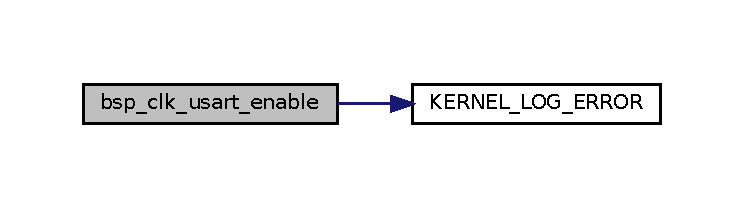
\includegraphics[width=350pt]{bsp__clocks_8c_aaf01af602e17579af5e6af009ae7a557_cgraph}
\end{center}
\end{figure}
Here is the caller graph for this function\+:\nopagebreak
\begin{figure}[H]
\begin{center}
\leavevmode
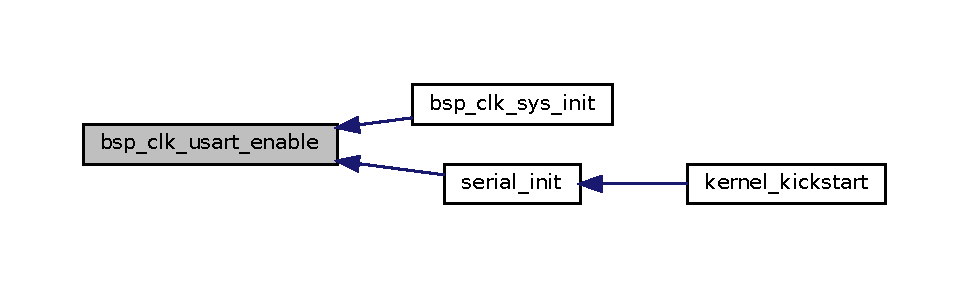
\includegraphics[width=350pt]{bsp__clocks_8c_aaf01af602e17579af5e6af009ae7a557_icgraph}
\end{center}
\end{figure}
\mbox{\Hypertarget{bsp__clocks_8c_ac154ab5d2a56dd8e09e0545e9775112e}\label{bsp__clocks_8c_ac154ab5d2a56dd8e09e0545e9775112e}} 
\index{bsp\+\_\+clocks.\+c@{bsp\+\_\+clocks.\+c}!bsp\+\_\+clock\+\_\+get\+\_\+pll\+\_\+freq@{bsp\+\_\+clock\+\_\+get\+\_\+pll\+\_\+freq}}
\index{bsp\+\_\+clock\+\_\+get\+\_\+pll\+\_\+freq@{bsp\+\_\+clock\+\_\+get\+\_\+pll\+\_\+freq}!bsp\+\_\+clocks.\+c@{bsp\+\_\+clocks.\+c}}
\subsubsection{\texorpdfstring{bsp\+\_\+clock\+\_\+get\+\_\+pll\+\_\+freq()}{bsp\_clock\_get\_pll\_freq()}}
{\footnotesize\ttfamily static \hyperlink{stdint_8h_a324c5d28c0d82f502a234ab99efac87a}{uint32\+\_\+t} bsp\+\_\+clock\+\_\+get\+\_\+pll\+\_\+freq (\begin{DoxyParamCaption}\item[{void}]{ }\end{DoxyParamCaption})\hspace{0.3cm}{\ttfamily [static]}}



Get the P\+LL output frequency in M\+Hz. 

Reads the P\+LL registers and compute the current P\+LL output frequency. The frequency returned is expressed in M\+Hz.

\begin{DoxyReturn}{Returns}
The P\+LL output frequency in M\+Hz. 
\end{DoxyReturn}


Definition at line 113 of file bsp\+\_\+clocks.\+c.


\begin{DoxyCode}
114 \{
115     \hyperlink{stdint_8h_a324c5d28c0d82f502a234ab99efac87a}{uint32\_t} pll\_freq;
116 
117     \textcolor{comment}{/* Get Source clock */}
118     \textcolor{keywordflow}{if}((*\hyperlink{bsp__clocks_8h_ad2d60b66a5292f1c04c7c3ebfe9df335}{RCC\_PLLCFGR\_REGISTER} & \hyperlink{bsp__clocks_8h_a6c5c6a2e8d760ad7da85ae2c8076ee31}{RCC\_PLLCFGR\_PLLSRC\_MASK}) == 0)
119     \{
120         pll\_freq = \hyperlink{bsp__clocks_8h_ae89e6b2d1e86b7fb4831cb013ece2c52}{RCC\_HSI\_BASE\_FREQ};
121     \}
122     \textcolor{keywordflow}{else} 
123     \{
124         pll\_freq = \hyperlink{bsp__clocks_8h_a19d723f47200a1da259e9c147f2de258}{RCC\_HSE\_BASE\_FREQ};
125     \}
126 
127     \textcolor{comment}{/* Get PLLM value */}
128     pll\_freq /= (*\hyperlink{bsp__clocks_8h_ad2d60b66a5292f1c04c7c3ebfe9df335}{RCC\_PLLCFGR\_REGISTER} & 
      \hyperlink{bsp__clocks_8h_afaac3bc429eaa475ca5e431a020d4c67}{RCC\_PLLCFGR\_PLLM\_MASK}) >> 
129                  \hyperlink{bsp__clocks_8h_add5fc49687031bdd44fca9c909f74fe0}{RCC\_PLLCFGR\_PLLM\_OFFSET};
130     \textcolor{comment}{/* Get PLLN value */}
131     pll\_freq *= (*\hyperlink{bsp__clocks_8h_ad2d60b66a5292f1c04c7c3ebfe9df335}{RCC\_PLLCFGR\_REGISTER} & 
      \hyperlink{bsp__clocks_8h_a90997335764397eb4be02c23676cda4a}{RCC\_PLLCFGR\_PLLN\_MASK}) >> 
132                  \hyperlink{bsp__clocks_8h_adc0f70732fb3d933c96d741f27baec35}{RCC\_PLLCFGR\_PLLN\_OFFSET};
133     \textcolor{comment}{/* Get PLLP value */}
134     pll\_freq /= (((*\hyperlink{bsp__clocks_8h_ad2d60b66a5292f1c04c7c3ebfe9df335}{RCC\_PLLCFGR\_REGISTER} & 
      \hyperlink{bsp__clocks_8h_a40a7c5938dfdd0ab63dcf3b203da7dd4}{RCC\_PLLCFGR\_PLLP\_MASK}) >> 
135                  \hyperlink{bsp__clocks_8h_a9a6c6234e6c59e7638d1a8edd237f591}{RCC\_PLLCFGR\_PLLP\_OFFSET}) + 1) * 2;
136     
137     \textcolor{keywordflow}{return} pll\_freq;
138 \}
\end{DoxyCode}
Here is the caller graph for this function\+:
\nopagebreak
\begin{figure}[H]
\begin{center}
\leavevmode
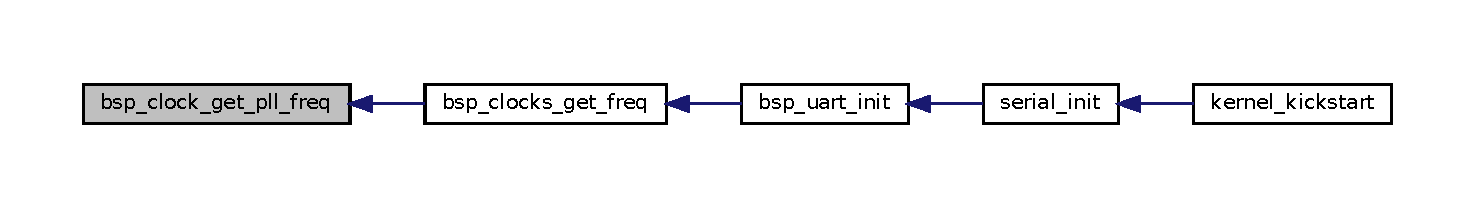
\includegraphics[width=350pt]{bsp__clocks_8c_ac154ab5d2a56dd8e09e0545e9775112e_icgraph}
\end{center}
\end{figure}
\mbox{\Hypertarget{bsp__clocks_8c_aeeded4b587684fa3383b3d42ee29af1e}\label{bsp__clocks_8c_aeeded4b587684fa3383b3d42ee29af1e}} 
\index{bsp\+\_\+clocks.\+c@{bsp\+\_\+clocks.\+c}!bsp\+\_\+clocks\+\_\+get\+\_\+freq@{bsp\+\_\+clocks\+\_\+get\+\_\+freq}}
\index{bsp\+\_\+clocks\+\_\+get\+\_\+freq@{bsp\+\_\+clocks\+\_\+get\+\_\+freq}!bsp\+\_\+clocks.\+c@{bsp\+\_\+clocks.\+c}}
\subsubsection{\texorpdfstring{bsp\+\_\+clocks\+\_\+get\+\_\+freq()}{bsp\_clocks\_get\_freq()}}
{\footnotesize\ttfamily \hyperlink{stdint_8h_a324c5d28c0d82f502a234ab99efac87a}{uint32\+\_\+t} bsp\+\_\+clocks\+\_\+get\+\_\+freq (\begin{DoxyParamCaption}\item[{const \hyperlink{bsp__clocks_8h_ac9d4d589a659370f313ef156f6eff0e8}{C\+L\+O\+C\+K\+\_\+\+I\+D\+E\+N\+T\+I\+F\+I\+E\+R\+\_\+T}}]{clk\+\_\+id }\end{DoxyParamCaption})}



Get the frequencies in M\+Hz of the clocks which identifer corresponds to the identifier given as parameter. 

Get the frequencies of the clocks which identifer corresponds to the identifier given as parameter. The P\+LL parameters and other clocks register are read to return the correct frequency for a given clock.


\begin{DoxyParams}[1]{Parameters}
\mbox{\tt in}  & {\em clk\+\_\+id} & The identifier of the clock.\\
\hline
\end{DoxyParams}
\begin{DoxyReturn}{Returns}
The frequency in M\+Hz of the clock is returned. 
\end{DoxyReturn}


Definition at line 307 of file bsp\+\_\+clocks.\+c.


\begin{DoxyCode}
308 \{
309     \hyperlink{stdint_8h_a324c5d28c0d82f502a234ab99efac87a}{uint32\_t} sysclk;
310     \hyperlink{stdint_8h_a324c5d28c0d82f502a234ab99efac87a}{uint32\_t} factor;
311 
312     \textcolor{comment}{/* Get Source clock */}
313     \textcolor{keywordflow}{if}((*\hyperlink{bsp__clocks_8h_ac454715dd9c4f8ba957cc53f318c58ac}{RCC\_CFGR\_REGISTER} & \hyperlink{bsp__clocks_8h_a451045d952eb1caaa0090c9e8dc75082}{RCC\_CFGR\_SWS\_MASK}) == 
      \hyperlink{bsp__clocks_8h_a2c67e2279804a83ef24438267d9d4a6c}{RCC\_CFGR\_SWS\_PLL})
314     \{
315         sysclk = \hyperlink{bsp__clocks_8c_ac154ab5d2a56dd8e09e0545e9775112e}{bsp\_clock\_get\_pll\_freq}();
316     \}
317     \textcolor{keywordflow}{else} \textcolor{keywordflow}{if}((*\hyperlink{bsp__clocks_8h_ac454715dd9c4f8ba957cc53f318c58ac}{RCC\_CFGR\_REGISTER} & RCC\_CFGR\_SWS\_MASK) == 
      \hyperlink{bsp__clocks_8h_a6764639cf221e1ebc0b5448dcaed590a}{RCC\_CFGR\_SWS\_HSI})
318     \{
319         sysclk = \hyperlink{bsp__clocks_8h_ae89e6b2d1e86b7fb4831cb013ece2c52}{RCC\_HSI\_BASE\_FREQ};
320     \}
321     \textcolor{keywordflow}{else} \textcolor{keywordflow}{if}((*\hyperlink{bsp__clocks_8h_ac454715dd9c4f8ba957cc53f318c58ac}{RCC\_CFGR\_REGISTER} & RCC\_CFGR\_SWS\_MASK) == 
      \hyperlink{bsp__clocks_8h_ae09a0202f441c1a43e69c62331d50a08}{RCC\_CFGR\_SWS\_HSE})
322     \{
323         sysclk = \hyperlink{bsp__clocks_8h_a19d723f47200a1da259e9c147f2de258}{RCC\_HSE\_BASE\_FREQ};
324     \}
325     \textcolor{keywordflow}{else} 
326     \{
327         \textcolor{comment}{/* We were  not able to detect the input clock */}
328         \textcolor{keywordflow}{return} 0;
329     \}
330 
331     \textcolor{comment}{/* Divide by AHB prescaler */}
332     \textcolor{keywordflow}{if}((*\hyperlink{bsp__clocks_8h_ac454715dd9c4f8ba957cc53f318c58ac}{RCC\_CFGR\_REGISTER} & \hyperlink{bsp__clocks_8h_a1351ccf5f6a5d9a6b91c4f533688d8fb}{RCC\_CFGR\_HPRE\_EN}) != 0)
333     \{
334         factor = (*\hyperlink{bsp__clocks_8h_ac454715dd9c4f8ba957cc53f318c58ac}{RCC\_CFGR\_REGISTER} & \hyperlink{bsp__clocks_8h_a2ff38fa14905e578752b706e5c29b146}{RCC\_CFGR\_HPRE\_VAL\_MASK}) >> 
335                   \hyperlink{bsp__clocks_8h_adca5b474c16bb5c9b4bbedfabeba8e25}{RCC\_CFGR\_HRPE\_OFFSET};
336         sysclk /= (\hyperlink{stdint_8h_a324c5d28c0d82f502a234ab99efac87a}{uint32\_t})\hyperlink{bsp__clocks_8c_abed7da9c2bfa6c8191c3bf928e64041f}{bsp\_hpre\_factor\_lookup}[factor];
337     \}
338 
339     \textcolor{keywordflow}{if}(clk\_id == \hyperlink{bsp__clocks_8h_ad0e92b49c1a7205e3460ca1e54fa9d70a58357d0569548d6c2ba44f27e0aa6ba6}{BSP\_CLOCK\_ID\_HCLK} || clk\_id == 
      \hyperlink{bsp__clocks_8h_ad0e92b49c1a7205e3460ca1e54fa9d70a265c9dec4478eb66904a2dbc6954e598}{BSP\_CLOCK\_ID\_FCLK})
340     \{
341         \textcolor{keywordflow}{return} sysclk;
342     \}
343     \textcolor{keywordflow}{else} \textcolor{keywordflow}{if}(clk\_id == \hyperlink{bsp__clocks_8h_ad0e92b49c1a7205e3460ca1e54fa9d70a0493d0bbd7edf1aebadb342c5c38f709}{BSP\_CLOCK\_ID\_PCLK1} || clk\_id == 
      \hyperlink{bsp__clocks_8h_ad0e92b49c1a7205e3460ca1e54fa9d70aad46d3b8852f9a4d711c15164bf1c0d3}{BSP\_CLOCK\_ID\_APB1\_TIMER})
344     \{
345         \textcolor{comment}{/* Get the APB1 prescaler */}
346         \textcolor{keywordflow}{if}((*\hyperlink{bsp__clocks_8h_ac454715dd9c4f8ba957cc53f318c58ac}{RCC\_CFGR\_REGISTER} & \hyperlink{bsp__clocks_8h_a7a4503de78658d3271cb5494adc96e41}{RCC\_CFGR\_PPRE1\_EN}) != 0)
347         \{
348             factor = (*\hyperlink{bsp__clocks_8h_ac454715dd9c4f8ba957cc53f318c58ac}{RCC\_CFGR\_REGISTER} & 
      \hyperlink{bsp__clocks_8h_aebda6f102f65bc354b95232527021aba}{RCC\_CFGR\_PPRE1\_VAL\_MASK}) >> 
349                       \hyperlink{bsp__clocks_8h_a1f605f808c9ab7530142dd8808e83a22}{RCC\_CFGR\_PPRE1\_OFFSET};
350 
351             sysclk /= (\hyperlink{stdint_8h_a324c5d28c0d82f502a234ab99efac87a}{uint32\_t})\hyperlink{bsp__clocks_8c_a1ef2cd1399c95dbe65a524595da1fc5c}{bsp\_ppre\_factor\_lookup}[factor];
352 
353             \textcolor{keywordflow}{if}(clk\_id == \hyperlink{bsp__clocks_8h_ad0e92b49c1a7205e3460ca1e54fa9d70aad46d3b8852f9a4d711c15164bf1c0d3}{BSP\_CLOCK\_ID\_APB1\_TIMER})
354             \{
355                 sysclk *= 2;
356             \}
357         \}
358     \}
359     \textcolor{keywordflow}{else} \textcolor{keywordflow}{if}(clk\_id == \hyperlink{bsp__clocks_8h_ad0e92b49c1a7205e3460ca1e54fa9d70aad62d8c78d2b4617724a82ec190a33ee}{BSP\_CLOCK\_ID\_PCLK2} || clk\_id == 
      \hyperlink{bsp__clocks_8h_ad0e92b49c1a7205e3460ca1e54fa9d70a30cca3be6a7bad72d2c02e9b58ff4d50}{BSP\_CLOCK\_ID\_APB2\_TIMER})
360     \{
361         \textcolor{comment}{/* Get the APB2 prescaler */}
362         \textcolor{keywordflow}{if}((*\hyperlink{bsp__clocks_8h_ac454715dd9c4f8ba957cc53f318c58ac}{RCC\_CFGR\_REGISTER} & \hyperlink{bsp__clocks_8h_a1a384b58d9f246cb60ed0d0bfa92cbf4}{RCC\_CFGR\_PPRE2\_EN}) != 0)
363         \{
364             factor = (*\hyperlink{bsp__clocks_8h_ac454715dd9c4f8ba957cc53f318c58ac}{RCC\_CFGR\_REGISTER} & 
      \hyperlink{bsp__clocks_8h_adb27fe14c6c6c2cb20f13aaf86f0900a}{RCC\_CFGR\_PPRE2\_VAL\_MASK}) >> 
365                       \hyperlink{bsp__clocks_8h_a906e390883db586903c4b1144a182e47}{RCC\_CFGR\_PPRE2\_OFFSET};
366             sysclk /= \hyperlink{bsp__clocks_8c_a1ef2cd1399c95dbe65a524595da1fc5c}{bsp\_ppre\_factor\_lookup}[factor];
367 
368             \textcolor{keywordflow}{if}(clk\_id == \hyperlink{bsp__clocks_8h_ad0e92b49c1a7205e3460ca1e54fa9d70a30cca3be6a7bad72d2c02e9b58ff4d50}{BSP\_CLOCK\_ID\_APB2\_TIMER})
369             \{
370                 sysclk *= 2;
371             \}
372         \}
373     \}
374     \textcolor{keywordflow}{else} 
375     \{
376         sysclk = 0;
377     \}
378 
379 \textcolor{preprocessor}{#if KERNEL\_LOG\_LEVEL >= INFO\_LOG\_LEVEL
}
380     KERNEL\_LOG\_INFO(\textcolor{stringliteral}{"System clock frequency requested"}, 
381                     (\textcolor{keywordtype}{void}*)(\hyperlink{stdint_8h_a324c5d28c0d82f502a234ab99efac87a}{uint32\_t})sysclk, 
382                     \textcolor{keyword}{sizeof}(sysclk), 
383                     \hyperlink{error__types_8h_a4db9ee29f2ff83c71567c12f6bfbf28cabf350750d0d4fabd8954c0f1e9bbae94}{NO\_ERROR});
384 \textcolor{preprocessor}{#endif
}
385 
386     \textcolor{keywordflow}{return} sysclk;
387 \}
\end{DoxyCode}
Here is the call graph for this function\+:
\nopagebreak
\begin{figure}[H]
\begin{center}
\leavevmode
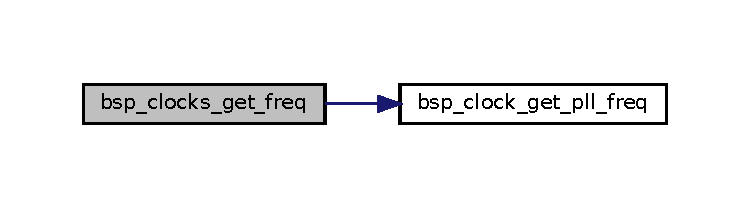
\includegraphics[width=350pt]{bsp__clocks_8c_aeeded4b587684fa3383b3d42ee29af1e_cgraph}
\end{center}
\end{figure}
Here is the caller graph for this function\+:
\nopagebreak
\begin{figure}[H]
\begin{center}
\leavevmode
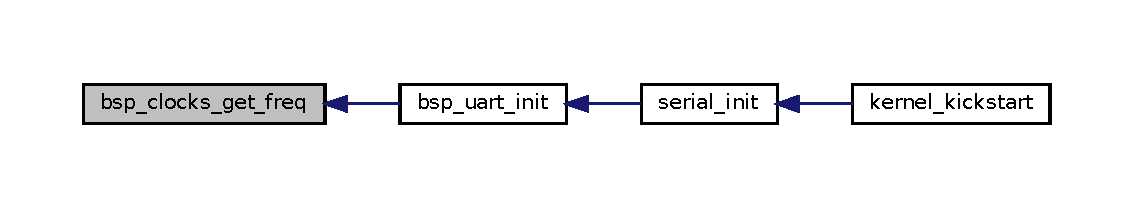
\includegraphics[width=350pt]{bsp__clocks_8c_aeeded4b587684fa3383b3d42ee29af1e_icgraph}
\end{center}
\end{figure}


\subsection{Variable Documentation}
\mbox{\Hypertarget{bsp__clocks_8c_a7e7b4728df96b76f3a8042b7fb46aa8c}\label{bsp__clocks_8c_a7e7b4728df96b76f3a8042b7fb46aa8c}} 
\index{bsp\+\_\+clocks.\+c@{bsp\+\_\+clocks.\+c}!bsp\+\_\+clk\+\_\+init@{bsp\+\_\+clk\+\_\+init}}
\index{bsp\+\_\+clk\+\_\+init@{bsp\+\_\+clk\+\_\+init}!bsp\+\_\+clocks.\+c@{bsp\+\_\+clocks.\+c}}
\subsubsection{\texorpdfstring{bsp\+\_\+clk\+\_\+init}{bsp\_clk\_init}}
{\footnotesize\ttfamily \hyperlink{stdint_8h_aba7bc1797add20fe3efdf37ced1182c5}{uint8\+\_\+t} bsp\+\_\+clk\+\_\+init = 0\hspace{0.3cm}{\ttfamily [static]}}



Stores the system clock init state. 



Definition at line 28 of file bsp\+\_\+clocks.\+c.

\mbox{\Hypertarget{bsp__clocks_8c_abed7da9c2bfa6c8191c3bf928e64041f}\label{bsp__clocks_8c_abed7da9c2bfa6c8191c3bf928e64041f}} 
\index{bsp\+\_\+clocks.\+c@{bsp\+\_\+clocks.\+c}!bsp\+\_\+hpre\+\_\+factor\+\_\+lookup@{bsp\+\_\+hpre\+\_\+factor\+\_\+lookup}}
\index{bsp\+\_\+hpre\+\_\+factor\+\_\+lookup@{bsp\+\_\+hpre\+\_\+factor\+\_\+lookup}!bsp\+\_\+clocks.\+c@{bsp\+\_\+clocks.\+c}}
\subsubsection{\texorpdfstring{bsp\+\_\+hpre\+\_\+factor\+\_\+lookup}{bsp\_hpre\_factor\_lookup}}
{\footnotesize\ttfamily const \hyperlink{stdint_8h_a273cf69d639a59973b6019625df33e30}{uint16\+\_\+t} bsp\+\_\+hpre\+\_\+factor\+\_\+lookup\mbox{[}8\mbox{]} = \{2, 4, 8, 16, 64, 128, 256, 512\}\hspace{0.3cm}{\ttfamily [static]}}



H\+R\+PE A\+HB prescaler factors lookup table. 



Definition at line 31 of file bsp\+\_\+clocks.\+c.

\mbox{\Hypertarget{bsp__clocks_8c_a1ef2cd1399c95dbe65a524595da1fc5c}\label{bsp__clocks_8c_a1ef2cd1399c95dbe65a524595da1fc5c}} 
\index{bsp\+\_\+clocks.\+c@{bsp\+\_\+clocks.\+c}!bsp\+\_\+ppre\+\_\+factor\+\_\+lookup@{bsp\+\_\+ppre\+\_\+factor\+\_\+lookup}}
\index{bsp\+\_\+ppre\+\_\+factor\+\_\+lookup@{bsp\+\_\+ppre\+\_\+factor\+\_\+lookup}!bsp\+\_\+clocks.\+c@{bsp\+\_\+clocks.\+c}}
\subsubsection{\texorpdfstring{bsp\+\_\+ppre\+\_\+factor\+\_\+lookup}{bsp\_ppre\_factor\_lookup}}
{\footnotesize\ttfamily const \hyperlink{stdint_8h_aba7bc1797add20fe3efdf37ced1182c5}{uint8\+\_\+t} bsp\+\_\+ppre\+\_\+factor\+\_\+lookup\mbox{[}4\mbox{]} = \{2, 4, 8, 16\}\hspace{0.3cm}{\ttfamily [static]}}



P\+P\+RE prescaler factors lookup table. 



Definition at line 34 of file bsp\+\_\+clocks.\+c.


\hypertarget{bsp__flash_8c}{}\section{Kernel/\+Sources/arch/board/stm32/f401re/src/bsp\+\_\+flash.c File Reference}
\label{bsp__flash_8c}\index{Kernel/\+Sources/arch/board/stm32/f401re/src/bsp\+\_\+flash.\+c@{Kernel/\+Sources/arch/board/stm32/f401re/src/bsp\+\_\+flash.\+c}}
{\ttfamily \#include \char`\"{}error\+\_\+types.\+h\char`\"{}}\newline
{\ttfamily \#include \char`\"{}bsp\+\_\+flash.\+h\char`\"{}}\newline
{\ttfamily \#include \char`\"{}cpu\+\_\+api.\+h\char`\"{}}\newline
{\ttfamily \#include \char`\"{}stdint.\+h\char`\"{}}\newline
{\ttfamily \#include \char`\"{}config.\+h\char`\"{}}\newline
Include dependency graph for bsp\+\_\+flash.\+c\+:\nopagebreak
\begin{figure}[H]
\begin{center}
\leavevmode
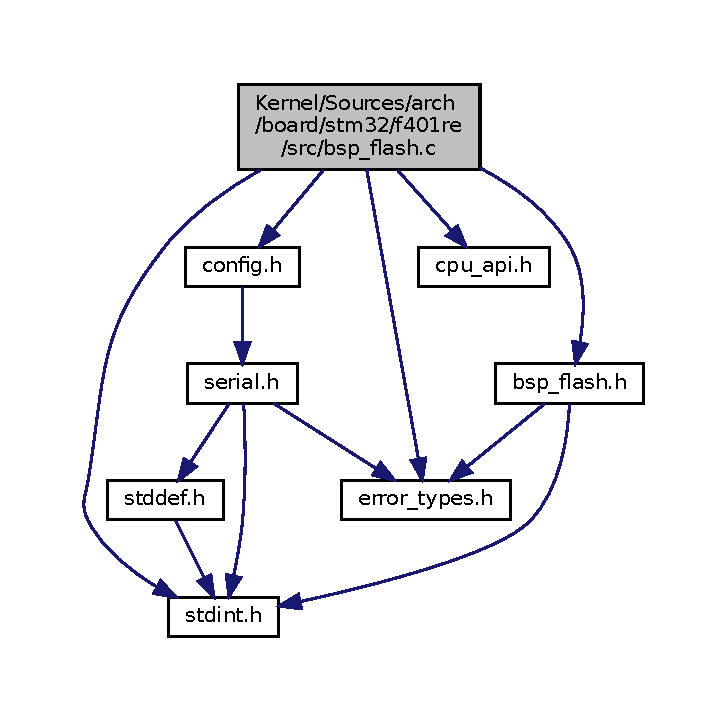
\includegraphics[width=349pt]{bsp__flash_8c__incl}
\end{center}
\end{figure}
\subsection*{Functions}
\begin{DoxyCompactItemize}
\item 
void \hyperlink{bsp__flash_8c_a28b133b49a8b54580ef07cc2b02b6a2d}{bsp\+\_\+flash\+\_\+cache\+\_\+enable} (void)
\begin{DoxyCompactList}\small\item\em Enables flash instruction and data cache. \end{DoxyCompactList}\item 
void \hyperlink{bsp__flash_8c_a2f8e8bffdc14c9ea45296defed4606a6}{bsp\+\_\+flash\+\_\+prefetch\+\_\+enable} (void)
\begin{DoxyCompactList}\small\item\em Enables flash prefetech unit. \end{DoxyCompactList}\item 
\hyperlink{error__types_8h_acf146bc98f60f47c79d782f7523e339c}{E\+R\+R\+O\+R\+\_\+\+C\+O\+D\+E\+\_\+E} \hyperlink{bsp__flash_8c_a51f3c79743adab8e26ca7a5c6b33c55b}{bsp\+\_\+flash\+\_\+set\+\_\+latency} (const \hyperlink{bsp__flash_8h_ab4bdf422e30b864e1ff48788fbde702d}{F\+L\+A\+S\+H\+\_\+\+L\+A\+T\+E\+N\+C\+Y\+\_\+\+W\+S\+\_\+E} latency)
\begin{DoxyCompactList}\small\item\em Sets the flash latency. \end{DoxyCompactList}\end{DoxyCompactItemize}


\subsection{Function Documentation}
\mbox{\Hypertarget{bsp__flash_8c_a28b133b49a8b54580ef07cc2b02b6a2d}\label{bsp__flash_8c_a28b133b49a8b54580ef07cc2b02b6a2d}} 
\index{bsp\+\_\+flash.\+c@{bsp\+\_\+flash.\+c}!bsp\+\_\+flash\+\_\+cache\+\_\+enable@{bsp\+\_\+flash\+\_\+cache\+\_\+enable}}
\index{bsp\+\_\+flash\+\_\+cache\+\_\+enable@{bsp\+\_\+flash\+\_\+cache\+\_\+enable}!bsp\+\_\+flash.\+c@{bsp\+\_\+flash.\+c}}
\subsubsection{\texorpdfstring{bsp\+\_\+flash\+\_\+cache\+\_\+enable()}{bsp\_flash\_cache\_enable()}}
{\footnotesize\ttfamily void bsp\+\_\+flash\+\_\+cache\+\_\+enable (\begin{DoxyParamCaption}\item[{void}]{ }\end{DoxyParamCaption})}



Enables flash instruction and data cache. 

­ $\ast$

Enables flash instruction and data cache. 

Definition at line 34 of file bsp\+\_\+flash.\+c.


\begin{DoxyCode}
35 \{
36     *\hyperlink{bsp__flash_8h_a177b682ed269b91b61bf46005fca9620}{FLASH\_ACR\_REGISTER} = *\hyperlink{bsp__flash_8h_a177b682ed269b91b61bf46005fca9620}{FLASH\_ACR\_REGISTER}  | 
37                            \hyperlink{bsp__flash_8h_a8723e738daa1eb5acfd3d66130060541}{FLASH\_ACR\_ICACHE\_EN} | 
38                            \hyperlink{bsp__flash_8h_a941d0c7a25f08c35724c4a572d90a6cc}{FLASH\_ACR\_DCACHE\_EN};
39     \hyperlink{cpu__api_8h_a386c6bcf8612ed54728c6157bb83036e}{cpu\_mem\_barrier}();
40 \}
\end{DoxyCode}
Here is the call graph for this function\+:\nopagebreak
\begin{figure}[H]
\begin{center}
\leavevmode
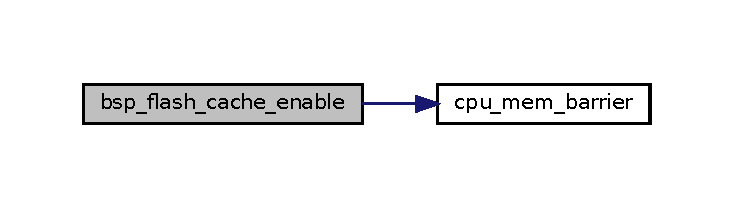
\includegraphics[width=350pt]{bsp__flash_8c_a28b133b49a8b54580ef07cc2b02b6a2d_cgraph}
\end{center}
\end{figure}
\mbox{\Hypertarget{bsp__flash_8c_a2f8e8bffdc14c9ea45296defed4606a6}\label{bsp__flash_8c_a2f8e8bffdc14c9ea45296defed4606a6}} 
\index{bsp\+\_\+flash.\+c@{bsp\+\_\+flash.\+c}!bsp\+\_\+flash\+\_\+prefetch\+\_\+enable@{bsp\+\_\+flash\+\_\+prefetch\+\_\+enable}}
\index{bsp\+\_\+flash\+\_\+prefetch\+\_\+enable@{bsp\+\_\+flash\+\_\+prefetch\+\_\+enable}!bsp\+\_\+flash.\+c@{bsp\+\_\+flash.\+c}}
\subsubsection{\texorpdfstring{bsp\+\_\+flash\+\_\+prefetch\+\_\+enable()}{bsp\_flash\_prefetch\_enable()}}
{\footnotesize\ttfamily void bsp\+\_\+flash\+\_\+prefetch\+\_\+enable (\begin{DoxyParamCaption}\item[{void}]{ }\end{DoxyParamCaption})}



Enables flash prefetech unit. 

­ $\ast$

Enables flash prefetech unit. 

Definition at line 42 of file bsp\+\_\+flash.\+c.


\begin{DoxyCode}
43 \{
44     *\hyperlink{bsp__flash_8h_a177b682ed269b91b61bf46005fca9620}{FLASH\_ACR\_REGISTER} = *\hyperlink{bsp__flash_8h_a177b682ed269b91b61bf46005fca9620}{FLASH\_ACR\_REGISTER}  |  
      \hyperlink{bsp__flash_8h_a479a3f068bb372bdf3bfc5b37846378a}{FLASH\_ACR\_PREFETCH\_EN};
45     \hyperlink{cpu__api_8h_a386c6bcf8612ed54728c6157bb83036e}{cpu\_mem\_barrier}();
46 \}
\end{DoxyCode}
Here is the call graph for this function\+:\nopagebreak
\begin{figure}[H]
\begin{center}
\leavevmode
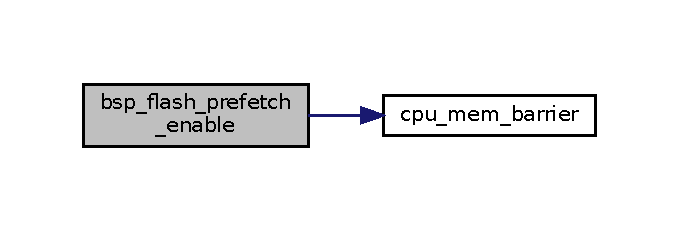
\includegraphics[width=326pt]{bsp__flash_8c_a2f8e8bffdc14c9ea45296defed4606a6_cgraph}
\end{center}
\end{figure}
\mbox{\Hypertarget{bsp__flash_8c_a51f3c79743adab8e26ca7a5c6b33c55b}\label{bsp__flash_8c_a51f3c79743adab8e26ca7a5c6b33c55b}} 
\index{bsp\+\_\+flash.\+c@{bsp\+\_\+flash.\+c}!bsp\+\_\+flash\+\_\+set\+\_\+latency@{bsp\+\_\+flash\+\_\+set\+\_\+latency}}
\index{bsp\+\_\+flash\+\_\+set\+\_\+latency@{bsp\+\_\+flash\+\_\+set\+\_\+latency}!bsp\+\_\+flash.\+c@{bsp\+\_\+flash.\+c}}
\subsubsection{\texorpdfstring{bsp\+\_\+flash\+\_\+set\+\_\+latency()}{bsp\_flash\_set\_latency()}}
{\footnotesize\ttfamily \hyperlink{error__types_8h_acf146bc98f60f47c79d782f7523e339c}{E\+R\+R\+O\+R\+\_\+\+C\+O\+D\+E\+\_\+E} bsp\+\_\+flash\+\_\+set\+\_\+latency (\begin{DoxyParamCaption}\item[{const \hyperlink{bsp__flash_8h_ab4bdf422e30b864e1ff48788fbde702d}{F\+L\+A\+S\+H\+\_\+\+L\+A\+T\+E\+N\+C\+Y\+\_\+\+W\+S\+\_\+E}}]{latency }\end{DoxyParamCaption})}



Sets the flash latency. 

­ $\ast$

Sets the flash latency based on the latency given as parameter.


\begin{DoxyParams}[1]{Parameters}
\mbox{\tt in}  & {\em latency} & The latency to set.\\
\hline
\end{DoxyParams}
\begin{DoxyReturn}{Returns}
N\+O\+\_\+\+E\+R\+R\+OR is returned in case of success. Otherwise an error code is returned. Please refer to the list of the standard error codes. 
\end{DoxyReturn}


Definition at line 48 of file bsp\+\_\+flash.\+c.


\begin{DoxyCode}
49 \{
50     \textcolor{comment}{/* Sets the flash latency value, we don't apply mask verification because 
}
51 \textcolor{comment}{     * the FLASH\_LATENCY\_WS\_E enumeration should already contain the right 
}
52 \textcolor{comment}{     * values.
}
53 \textcolor{comment}{     */}
54     *\hyperlink{bsp__flash_8h_a177b682ed269b91b61bf46005fca9620}{FLASH\_ACR\_REGISTER} = (*\hyperlink{bsp__flash_8h_a177b682ed269b91b61bf46005fca9620}{FLASH\_ACR\_REGISTER} & ~
      \hyperlink{bsp__flash_8h_a325fd0108f2a85889c495a9f08409216}{FLASH\_ACR\_LATENCY\_MASK}) | 
55                           latency;
56 
57     \textcolor{comment}{/* Delay to ensure bit update */}
58     \textcolor{keywordflow}{while}((*\hyperlink{bsp__flash_8h_a177b682ed269b91b61bf46005fca9620}{FLASH\_ACR\_REGISTER} & \hyperlink{bsp__flash_8h_a325fd0108f2a85889c495a9f08409216}{FLASH\_ACR\_LATENCY\_MASK}) != latency
      );
59 
60 \textcolor{preprocessor}{#if KERNEL\_LOG\_LEVEL >= INFO\_LOG\_LEVEL
}
61     KERNEL\_LOG\_INFO(\textcolor{stringliteral}{"Flash lantency changed"}, 
62                     latency, 
63                     \textcolor{keyword}{sizeof}(latency), 
64                     \hyperlink{error__types_8h_a4db9ee29f2ff83c71567c12f6bfbf28cabf350750d0d4fabd8954c0f1e9bbae94}{NO\_ERROR});
65 \textcolor{preprocessor}{#endif
}
66 
67     \textcolor{keywordflow}{return} \hyperlink{error__types_8h_a4db9ee29f2ff83c71567c12f6bfbf28cabf350750d0d4fabd8954c0f1e9bbae94}{NO\_ERROR};
68 \}
\end{DoxyCode}
Here is the caller graph for this function\+:\nopagebreak
\begin{figure}[H]
\begin{center}
\leavevmode
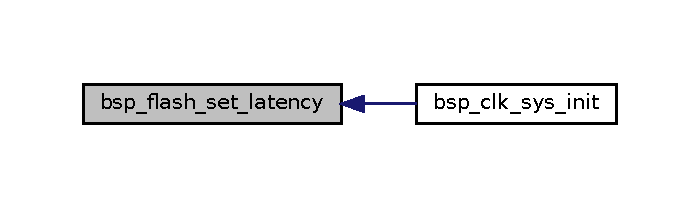
\includegraphics[width=336pt]{bsp__flash_8c_a51f3c79743adab8e26ca7a5c6b33c55b_icgraph}
\end{center}
\end{figure}

\hypertarget{bsp__gpio_8c}{}\section{Kernel/\+Sources/arch/board/stm32/f401re/src/bsp\+\_\+gpio.c File Reference}
\label{bsp__gpio_8c}\index{Kernel/\+Sources/arch/board/stm32/f401re/src/bsp\+\_\+gpio.\+c@{Kernel/\+Sources/arch/board/stm32/f401re/src/bsp\+\_\+gpio.\+c}}
{\ttfamily \#include \char`\"{}error\+\_\+types.\+h\char`\"{}}\newline
{\ttfamily \#include \char`\"{}bsp\+\_\+gpio.\+h\char`\"{}}\newline
{\ttfamily \#include \char`\"{}stdint.\+h\char`\"{}}\newline
{\ttfamily \#include \char`\"{}config.\+h\char`\"{}}\newline
{\ttfamily \#include \char`\"{}stddef.\+h\char`\"{}}\newline
{\ttfamily \#include \char`\"{}logger.\+h\char`\"{}}\newline
Include dependency graph for bsp\+\_\+gpio.\+c\+:\nopagebreak
\begin{figure}[H]
\begin{center}
\leavevmode
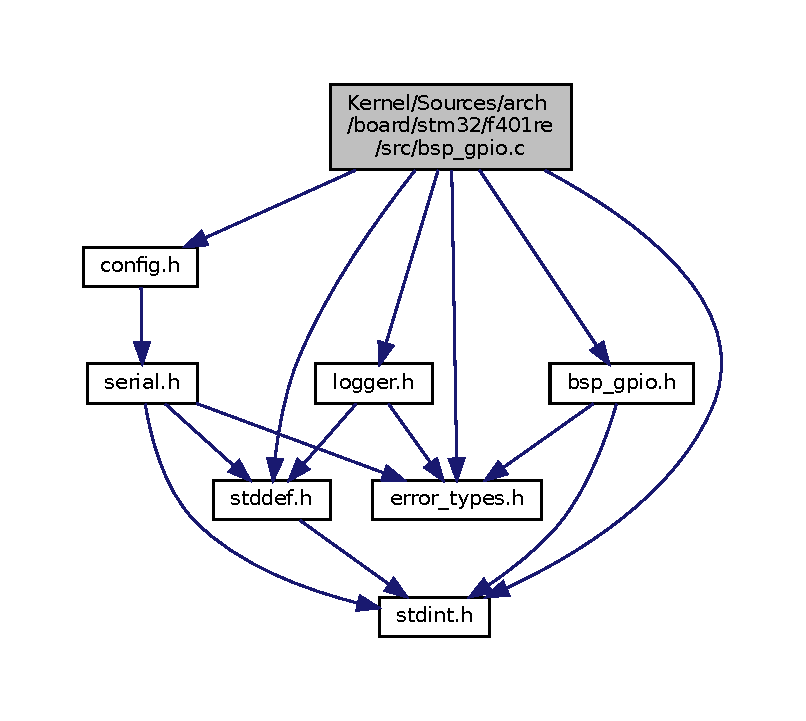
\includegraphics[width=350pt]{bsp__gpio_8c__incl}
\end{center}
\end{figure}
\subsection*{Macros}
\begin{DoxyCompactItemize}
\item 
\#define \hyperlink{bsp__gpio_8c_ae8e3e4a5297b1359f01d8a77bcc270c0}{C\+H\+E\+C\+K\+\_\+\+M\+O\+D\+E\+T\+Y\+PE}(modetype)
\begin{DoxyCompactList}\small\item\em Checks the mode and type field conformity. \end{DoxyCompactList}\item 
\#define \hyperlink{bsp__gpio_8c_aabaa6421ac1a7a8e9d453628650ab7a3}{C\+H\+E\+C\+K\+\_\+\+S\+P\+E\+ED}(speed)
\begin{DoxyCompactList}\small\item\em Checks the speed field conformity. \end{DoxyCompactList}\item 
\#define \hyperlink{bsp__gpio_8c_a5ede3d69b9f41a22b2fc0beb806967d3}{C\+H\+E\+C\+K\+\_\+\+A\+L\+T\+F\+U\+NC}(altfunc)
\begin{DoxyCompactList}\small\item\em Checks the alternate function field conformity. \end{DoxyCompactList}\item 
\#define \hyperlink{bsp__gpio_8c_a56f1639d4d0edda81bed942e0a536b3d}{G\+P\+I\+O\+\_\+\+X\+\_\+\+R\+E\+G\+I\+S\+T\+ER}(gpio,  offset)~((volatile \hyperlink{stdint_8h_a324c5d28c0d82f502a234ab99efac87a}{uint32\+\_\+t}$\ast$)(\hyperlink{bsp__gpio_8h_a72db53eb21962c0c32457008d0e0b3bf}{G\+P\+I\+O\+\_\+\+X\+\_\+\+B\+A\+S\+E\+\_\+\+A\+D\+D\+R\+E\+SS} + 0x400 $\ast$ gpio + offset))
\begin{DoxyCompactList}\small\item\em Computes the register address for a given G\+P\+IO register. \end{DoxyCompactList}\item 
\#define \hyperlink{bsp__gpio_8c_a70e4ad259c3ad36b511918978e23c9ad}{G\+P\+I\+O\+\_\+\+O\+T\+Y\+P\+E\+R\+\_\+\+M\+A\+SK}(pin)~(1 $<$$<$ pin)
\begin{DoxyCompactList}\small\item\em computed the output type field mask for a given G\+P\+IO pin. \end{DoxyCompactList}\item 
\#define \hyperlink{bsp__gpio_8c_a8a5c19e32e8c8d3951f2bcb27839eedd}{G\+P\+I\+O\+\_\+\+O\+S\+P\+E\+E\+D\+R\+\_\+\+M\+A\+SK}(pin)~(1 $<$$<$ (pin $<$$<$ 1))
\begin{DoxyCompactList}\small\item\em computed the output speed field mask for a given G\+P\+IO pin. \end{DoxyCompactList}\item 
\#define \hyperlink{bsp__gpio_8c_a0900dad3061f961852cfccc1c2113b78}{G\+P\+I\+O\+\_\+\+A\+F\+R\+\_\+\+M\+A\+SK}(pin)~(1 $<$$<$ (pin $<$$<$ 2))
\begin{DoxyCompactList}\small\item\em computed the A\+FR field mask for a given G\+P\+IO pin. \end{DoxyCompactList}\item 
\#define \hyperlink{bsp__gpio_8c_a4528590820ddd2bbefba27ed999298b4}{G\+P\+I\+O\+\_\+\+M\+O\+D\+E\+R\+\_\+\+M\+A\+SK}(pin)~(1 $<$$<$ (pin $<$$<$ 1))
\begin{DoxyCompactList}\small\item\em computed the mode field mask for a given G\+P\+IO pin. \end{DoxyCompactList}\item 
\#define \hyperlink{bsp__gpio_8c_a18ae923766f6495859f915dfb671f19a}{G\+P\+I\+O\+\_\+\+P\+U\+P\+D\+R\+\_\+\+M\+A\+SK}(pin)~(1 $<$$<$ (pin $<$$<$ 1))
\begin{DoxyCompactList}\small\item\em computed the P\+U\+PD field mask for a given G\+P\+IO pin. \end{DoxyCompactList}\end{DoxyCompactItemize}
\subsection*{Functions}
\begin{DoxyCompactItemize}
\item 
\hyperlink{error__types_8h_acf146bc98f60f47c79d782f7523e339c}{E\+R\+R\+O\+R\+\_\+\+C\+O\+D\+E\+\_\+E} \hyperlink{bsp__gpio_8c_ac05d93f29cf8cdcd3809298fe5df2f87}{bsp\+\_\+gpio\+\_\+init} (const \hyperlink{bsp__gpio_8h_ab086506332275a2a873dfce02ed5a3b8}{G\+P\+I\+O\+\_\+\+I\+D\+E\+N\+T\+I\+F\+I\+E\+R\+\_\+E} gpio\+\_\+id, const \hyperlink{bsp__gpio_8h_ad7cd0faab6d093c8c9c399372e147467}{G\+P\+I\+O\+\_\+\+S\+E\+T\+T\+I\+N\+G\+S\+\_\+T} $\ast$settings)
\begin{DoxyCompactList}\small\item\em Initializes a given G\+P\+IO bank. \end{DoxyCompactList}\end{DoxyCompactItemize}


\subsection{Macro Definition Documentation}
\mbox{\Hypertarget{bsp__gpio_8c_a5ede3d69b9f41a22b2fc0beb806967d3}\label{bsp__gpio_8c_a5ede3d69b9f41a22b2fc0beb806967d3}} 
\index{bsp\+\_\+gpio.\+c@{bsp\+\_\+gpio.\+c}!C\+H\+E\+C\+K\+\_\+\+A\+L\+T\+F\+U\+NC@{C\+H\+E\+C\+K\+\_\+\+A\+L\+T\+F\+U\+NC}}
\index{C\+H\+E\+C\+K\+\_\+\+A\+L\+T\+F\+U\+NC@{C\+H\+E\+C\+K\+\_\+\+A\+L\+T\+F\+U\+NC}!bsp\+\_\+gpio.\+c@{bsp\+\_\+gpio.\+c}}
\subsubsection{\texorpdfstring{C\+H\+E\+C\+K\+\_\+\+A\+L\+T\+F\+U\+NC}{CHECK\_ALTFUNC}}
{\footnotesize\ttfamily \#define C\+H\+E\+C\+K\+\_\+\+A\+L\+T\+F\+U\+NC(\begin{DoxyParamCaption}\item[{}]{altfunc }\end{DoxyParamCaption})}

{\bfseries Value\+:}
\begin{DoxyCode}
(\{                                                                           \(\backslash\)
    if(altfunc > \hyperlink{bsp__gpio_8h_ad08e321e0fe351c401c3c698bba92fd7}{GPIO\_ALFUNC\_15})                                             \(\backslash\)
    \{                                                                        \(\backslash\)
        if(\hyperlink{config_8h_a6c272d2b12ffba9bdd5a4d5dd608a0f8}{KERNEL\_LOG\_LEVEL} == \hyperlink{config_8h_a023f94f341f2300adee0891b15b364b2}{ERROR\_LOG\_LEVEL})                             
       \(\backslash\)
        \{                                                                    \(\backslash\)
            KERNEL\_LOG\_ERROR(\textcolor{stringliteral}{"Invalid GPIO alternative function"},            \(\backslash\)
                             (\textcolor{keywordtype}{void}*)(\hyperlink{stdint_8h_a324c5d28c0d82f502a234ab99efac87a}{uint32\_t})altfunc,                       \(\backslash\)
                             \textcolor{keyword}{sizeof}(altfunc),                                \(\backslash\)
                             \hyperlink{error__types_8h_a4db9ee29f2ff83c71567c12f6bfbf28cabbe6797281350f36c23d07d6f2d7f6e2}{ERROR\_INVALID\_PARAM});                           \(\backslash\)
        \}                                                                    \(\backslash\)
                                                                             \(\backslash\)
        return \hyperlink{error__types_8h_a4db9ee29f2ff83c71567c12f6bfbf28cabbe6797281350f36c23d07d6f2d7f6e2}{ERROR\_INVALID\_PARAM};                                          \(\backslash\)
    \}                                                                        \(\backslash\)
\})
\end{DoxyCode}


Checks the alternate function field conformity. 

This macro will return from the function it is used in if an error is detected. An error message will be logged and an invalid parameter error is returned.


\begin{DoxyParams}[1]{Parameters}
\mbox{\tt in}  & {\em altfunc} & The alternate function of the G\+P\+IO settings. \\
\hline
\end{DoxyParams}


Definition at line 119 of file bsp\+\_\+gpio.\+c.

\mbox{\Hypertarget{bsp__gpio_8c_ae8e3e4a5297b1359f01d8a77bcc270c0}\label{bsp__gpio_8c_ae8e3e4a5297b1359f01d8a77bcc270c0}} 
\index{bsp\+\_\+gpio.\+c@{bsp\+\_\+gpio.\+c}!C\+H\+E\+C\+K\+\_\+\+M\+O\+D\+E\+T\+Y\+PE@{C\+H\+E\+C\+K\+\_\+\+M\+O\+D\+E\+T\+Y\+PE}}
\index{C\+H\+E\+C\+K\+\_\+\+M\+O\+D\+E\+T\+Y\+PE@{C\+H\+E\+C\+K\+\_\+\+M\+O\+D\+E\+T\+Y\+PE}!bsp\+\_\+gpio.\+c@{bsp\+\_\+gpio.\+c}}
\subsubsection{\texorpdfstring{C\+H\+E\+C\+K\+\_\+\+M\+O\+D\+E\+T\+Y\+PE}{CHECK\_MODETYPE}}
{\footnotesize\ttfamily \#define C\+H\+E\+C\+K\+\_\+\+M\+O\+D\+E\+T\+Y\+PE(\begin{DoxyParamCaption}\item[{}]{modetype }\end{DoxyParamCaption})}



Checks the mode and type field conformity. 

This macro will return from the function it is used in if an error is detected. An error message will be logged and an invalid parameter error is returned.


\begin{DoxyParams}[1]{Parameters}
\mbox{\tt in}  & {\em modetype} & The mode and type of the G\+P\+IO settings. \\
\hline
\end{DoxyParams}


Definition at line 40 of file bsp\+\_\+gpio.\+c.

\mbox{\Hypertarget{bsp__gpio_8c_aabaa6421ac1a7a8e9d453628650ab7a3}\label{bsp__gpio_8c_aabaa6421ac1a7a8e9d453628650ab7a3}} 
\index{bsp\+\_\+gpio.\+c@{bsp\+\_\+gpio.\+c}!C\+H\+E\+C\+K\+\_\+\+S\+P\+E\+ED@{C\+H\+E\+C\+K\+\_\+\+S\+P\+E\+ED}}
\index{C\+H\+E\+C\+K\+\_\+\+S\+P\+E\+ED@{C\+H\+E\+C\+K\+\_\+\+S\+P\+E\+ED}!bsp\+\_\+gpio.\+c@{bsp\+\_\+gpio.\+c}}
\subsubsection{\texorpdfstring{C\+H\+E\+C\+K\+\_\+\+S\+P\+E\+ED}{CHECK\_SPEED}}
{\footnotesize\ttfamily \#define C\+H\+E\+C\+K\+\_\+\+S\+P\+E\+ED(\begin{DoxyParamCaption}\item[{}]{speed }\end{DoxyParamCaption})}

{\bfseries Value\+:}
\begin{DoxyCode}
(\{                                                                           \(\backslash\)
    if(speed > \hyperlink{bsp__gpio_8h_ae11603e44b5bb26398c583a2410cafd5}{GPIO\_SPEED\_VERY\_HIGH})                                         \(\backslash\)
    \{                                                                        \(\backslash\)
        if(\hyperlink{config_8h_a6c272d2b12ffba9bdd5a4d5dd608a0f8}{KERNEL\_LOG\_LEVEL} == \hyperlink{config_8h_a023f94f341f2300adee0891b15b364b2}{ERROR\_LOG\_LEVEL})                             
       \(\backslash\)
        \{                                                                    \(\backslash\)
            KERNEL\_LOG\_ERROR(\textcolor{stringliteral}{"Invalid GPIO speed"},                           \(\backslash\)
                             (\textcolor{keywordtype}{void}*)(\hyperlink{stdint_8h_a324c5d28c0d82f502a234ab99efac87a}{uint32\_t})speed,                         \(\backslash\)
                             \textcolor{keyword}{sizeof}(speed),                                  \(\backslash\)
                             \hyperlink{error__types_8h_a4db9ee29f2ff83c71567c12f6bfbf28cabbe6797281350f36c23d07d6f2d7f6e2}{ERROR\_INVALID\_PARAM});                           \(\backslash\)
        \}                                                                    \(\backslash\)
                                                                             \(\backslash\)
        return \hyperlink{error__types_8h_a4db9ee29f2ff83c71567c12f6bfbf28cabbe6797281350f36c23d07d6f2d7f6e2}{ERROR\_INVALID\_PARAM};                                          \(\backslash\)
    \}                                                                        \(\backslash\)
\})
\end{DoxyCode}


Checks the speed field conformity. 

This macro will return from the function it is used in if an error is detected. An error message will be logged and an invalid parameter error is returned.


\begin{DoxyParams}[1]{Parameters}
\mbox{\tt in}  & {\em speed} & The speed of the G\+P\+IO settings. \\
\hline
\end{DoxyParams}


Definition at line 94 of file bsp\+\_\+gpio.\+c.

\mbox{\Hypertarget{bsp__gpio_8c_a0900dad3061f961852cfccc1c2113b78}\label{bsp__gpio_8c_a0900dad3061f961852cfccc1c2113b78}} 
\index{bsp\+\_\+gpio.\+c@{bsp\+\_\+gpio.\+c}!G\+P\+I\+O\+\_\+\+A\+F\+R\+\_\+\+M\+A\+SK@{G\+P\+I\+O\+\_\+\+A\+F\+R\+\_\+\+M\+A\+SK}}
\index{G\+P\+I\+O\+\_\+\+A\+F\+R\+\_\+\+M\+A\+SK@{G\+P\+I\+O\+\_\+\+A\+F\+R\+\_\+\+M\+A\+SK}!bsp\+\_\+gpio.\+c@{bsp\+\_\+gpio.\+c}}
\subsubsection{\texorpdfstring{G\+P\+I\+O\+\_\+\+A\+F\+R\+\_\+\+M\+A\+SK}{GPIO\_AFR\_MASK}}
{\footnotesize\ttfamily \#define G\+P\+I\+O\+\_\+\+A\+F\+R\+\_\+\+M\+A\+SK(\begin{DoxyParamCaption}\item[{}]{pin }\end{DoxyParamCaption})~(1 $<$$<$ (pin $<$$<$ 2))}



computed the A\+FR field mask for a given G\+P\+IO pin. 


\begin{DoxyParams}[1]{Parameters}
\mbox{\tt in}  & {\em pin} & The pin number for wich we compute the A\+FR field mask.\\
\hline
\end{DoxyParams}
\begin{DoxyReturn}{Returns}
The A\+FR field mask is computed. 
\end{DoxyReturn}


Definition at line 170 of file bsp\+\_\+gpio.\+c.

\mbox{\Hypertarget{bsp__gpio_8c_a4528590820ddd2bbefba27ed999298b4}\label{bsp__gpio_8c_a4528590820ddd2bbefba27ed999298b4}} 
\index{bsp\+\_\+gpio.\+c@{bsp\+\_\+gpio.\+c}!G\+P\+I\+O\+\_\+\+M\+O\+D\+E\+R\+\_\+\+M\+A\+SK@{G\+P\+I\+O\+\_\+\+M\+O\+D\+E\+R\+\_\+\+M\+A\+SK}}
\index{G\+P\+I\+O\+\_\+\+M\+O\+D\+E\+R\+\_\+\+M\+A\+SK@{G\+P\+I\+O\+\_\+\+M\+O\+D\+E\+R\+\_\+\+M\+A\+SK}!bsp\+\_\+gpio.\+c@{bsp\+\_\+gpio.\+c}}
\subsubsection{\texorpdfstring{G\+P\+I\+O\+\_\+\+M\+O\+D\+E\+R\+\_\+\+M\+A\+SK}{GPIO\_MODER\_MASK}}
{\footnotesize\ttfamily \#define G\+P\+I\+O\+\_\+\+M\+O\+D\+E\+R\+\_\+\+M\+A\+SK(\begin{DoxyParamCaption}\item[{}]{pin }\end{DoxyParamCaption})~(1 $<$$<$ (pin $<$$<$ 1))}



computed the mode field mask for a given G\+P\+IO pin. 


\begin{DoxyParams}[1]{Parameters}
\mbox{\tt in}  & {\em pin} & The pin number for wich we compute the mode field mask.\\
\hline
\end{DoxyParams}
\begin{DoxyReturn}{Returns}
The mode field mask is computed. 
\end{DoxyReturn}


Definition at line 178 of file bsp\+\_\+gpio.\+c.

\mbox{\Hypertarget{bsp__gpio_8c_a8a5c19e32e8c8d3951f2bcb27839eedd}\label{bsp__gpio_8c_a8a5c19e32e8c8d3951f2bcb27839eedd}} 
\index{bsp\+\_\+gpio.\+c@{bsp\+\_\+gpio.\+c}!G\+P\+I\+O\+\_\+\+O\+S\+P\+E\+E\+D\+R\+\_\+\+M\+A\+SK@{G\+P\+I\+O\+\_\+\+O\+S\+P\+E\+E\+D\+R\+\_\+\+M\+A\+SK}}
\index{G\+P\+I\+O\+\_\+\+O\+S\+P\+E\+E\+D\+R\+\_\+\+M\+A\+SK@{G\+P\+I\+O\+\_\+\+O\+S\+P\+E\+E\+D\+R\+\_\+\+M\+A\+SK}!bsp\+\_\+gpio.\+c@{bsp\+\_\+gpio.\+c}}
\subsubsection{\texorpdfstring{G\+P\+I\+O\+\_\+\+O\+S\+P\+E\+E\+D\+R\+\_\+\+M\+A\+SK}{GPIO\_OSPEEDR\_MASK}}
{\footnotesize\ttfamily \#define G\+P\+I\+O\+\_\+\+O\+S\+P\+E\+E\+D\+R\+\_\+\+M\+A\+SK(\begin{DoxyParamCaption}\item[{}]{pin }\end{DoxyParamCaption})~(1 $<$$<$ (pin $<$$<$ 1))}



computed the output speed field mask for a given G\+P\+IO pin. 


\begin{DoxyParams}[1]{Parameters}
\mbox{\tt in}  & {\em pin} & The pin number for wich we compute the output speed field mask.\\
\hline
\end{DoxyParams}
\begin{DoxyReturn}{Returns}
The output speed field mask is computed. 
\end{DoxyReturn}


Definition at line 162 of file bsp\+\_\+gpio.\+c.

\mbox{\Hypertarget{bsp__gpio_8c_a70e4ad259c3ad36b511918978e23c9ad}\label{bsp__gpio_8c_a70e4ad259c3ad36b511918978e23c9ad}} 
\index{bsp\+\_\+gpio.\+c@{bsp\+\_\+gpio.\+c}!G\+P\+I\+O\+\_\+\+O\+T\+Y\+P\+E\+R\+\_\+\+M\+A\+SK@{G\+P\+I\+O\+\_\+\+O\+T\+Y\+P\+E\+R\+\_\+\+M\+A\+SK}}
\index{G\+P\+I\+O\+\_\+\+O\+T\+Y\+P\+E\+R\+\_\+\+M\+A\+SK@{G\+P\+I\+O\+\_\+\+O\+T\+Y\+P\+E\+R\+\_\+\+M\+A\+SK}!bsp\+\_\+gpio.\+c@{bsp\+\_\+gpio.\+c}}
\subsubsection{\texorpdfstring{G\+P\+I\+O\+\_\+\+O\+T\+Y\+P\+E\+R\+\_\+\+M\+A\+SK}{GPIO\_OTYPER\_MASK}}
{\footnotesize\ttfamily \#define G\+P\+I\+O\+\_\+\+O\+T\+Y\+P\+E\+R\+\_\+\+M\+A\+SK(\begin{DoxyParamCaption}\item[{}]{pin }\end{DoxyParamCaption})~(1 $<$$<$ pin)}



computed the output type field mask for a given G\+P\+IO pin. 


\begin{DoxyParams}[1]{Parameters}
\mbox{\tt in}  & {\em pin} & The pin number for wich we compute the output type field mask.\\
\hline
\end{DoxyParams}
\begin{DoxyReturn}{Returns}
The output type field mask is computed. 
\end{DoxyReturn}


Definition at line 153 of file bsp\+\_\+gpio.\+c.

\mbox{\Hypertarget{bsp__gpio_8c_a18ae923766f6495859f915dfb671f19a}\label{bsp__gpio_8c_a18ae923766f6495859f915dfb671f19a}} 
\index{bsp\+\_\+gpio.\+c@{bsp\+\_\+gpio.\+c}!G\+P\+I\+O\+\_\+\+P\+U\+P\+D\+R\+\_\+\+M\+A\+SK@{G\+P\+I\+O\+\_\+\+P\+U\+P\+D\+R\+\_\+\+M\+A\+SK}}
\index{G\+P\+I\+O\+\_\+\+P\+U\+P\+D\+R\+\_\+\+M\+A\+SK@{G\+P\+I\+O\+\_\+\+P\+U\+P\+D\+R\+\_\+\+M\+A\+SK}!bsp\+\_\+gpio.\+c@{bsp\+\_\+gpio.\+c}}
\subsubsection{\texorpdfstring{G\+P\+I\+O\+\_\+\+P\+U\+P\+D\+R\+\_\+\+M\+A\+SK}{GPIO\_PUPDR\_MASK}}
{\footnotesize\ttfamily \#define G\+P\+I\+O\+\_\+\+P\+U\+P\+D\+R\+\_\+\+M\+A\+SK(\begin{DoxyParamCaption}\item[{}]{pin }\end{DoxyParamCaption})~(1 $<$$<$ (pin $<$$<$ 1))}



computed the P\+U\+PD field mask for a given G\+P\+IO pin. 


\begin{DoxyParams}[1]{Parameters}
\mbox{\tt in}  & {\em pin} & The pin number for wich we compute the P\+U\+PD field mask.\\
\hline
\end{DoxyParams}
\begin{DoxyReturn}{Returns}
The P\+U\+PD field mask is computed. 
\end{DoxyReturn}


Definition at line 186 of file bsp\+\_\+gpio.\+c.

\mbox{\Hypertarget{bsp__gpio_8c_a56f1639d4d0edda81bed942e0a536b3d}\label{bsp__gpio_8c_a56f1639d4d0edda81bed942e0a536b3d}} 
\index{bsp\+\_\+gpio.\+c@{bsp\+\_\+gpio.\+c}!G\+P\+I\+O\+\_\+\+X\+\_\+\+R\+E\+G\+I\+S\+T\+ER@{G\+P\+I\+O\+\_\+\+X\+\_\+\+R\+E\+G\+I\+S\+T\+ER}}
\index{G\+P\+I\+O\+\_\+\+X\+\_\+\+R\+E\+G\+I\+S\+T\+ER@{G\+P\+I\+O\+\_\+\+X\+\_\+\+R\+E\+G\+I\+S\+T\+ER}!bsp\+\_\+gpio.\+c@{bsp\+\_\+gpio.\+c}}
\subsubsection{\texorpdfstring{G\+P\+I\+O\+\_\+\+X\+\_\+\+R\+E\+G\+I\+S\+T\+ER}{GPIO\_X\_REGISTER}}
{\footnotesize\ttfamily \#define G\+P\+I\+O\+\_\+\+X\+\_\+\+R\+E\+G\+I\+S\+T\+ER(\begin{DoxyParamCaption}\item[{}]{gpio,  }\item[{}]{offset }\end{DoxyParamCaption})~((volatile \hyperlink{stdint_8h_a324c5d28c0d82f502a234ab99efac87a}{uint32\+\_\+t}$\ast$)(\hyperlink{bsp__gpio_8h_a72db53eb21962c0c32457008d0e0b3bf}{G\+P\+I\+O\+\_\+\+X\+\_\+\+B\+A\+S\+E\+\_\+\+A\+D\+D\+R\+E\+SS} + 0x400 $\ast$ gpio + offset))}



Computes the register address for a given G\+P\+IO register. 


\begin{DoxyParams}[1]{Parameters}
\mbox{\tt in}  & {\em gpio} & The identifier of the G\+P\+IO for wich we request the address. \\
\hline
\mbox{\tt in}  & {\em offset} & The G\+P\+IO register address offset.\\
\hline
\end{DoxyParams}
\begin{DoxyReturn}{Returns}
The register absolute address is computed. 
\end{DoxyReturn}


Definition at line 143 of file bsp\+\_\+gpio.\+c.



\subsection{Function Documentation}
\mbox{\Hypertarget{bsp__gpio_8c_ac05d93f29cf8cdcd3809298fe5df2f87}\label{bsp__gpio_8c_ac05d93f29cf8cdcd3809298fe5df2f87}} 
\index{bsp\+\_\+gpio.\+c@{bsp\+\_\+gpio.\+c}!bsp\+\_\+gpio\+\_\+init@{bsp\+\_\+gpio\+\_\+init}}
\index{bsp\+\_\+gpio\+\_\+init@{bsp\+\_\+gpio\+\_\+init}!bsp\+\_\+gpio.\+c@{bsp\+\_\+gpio.\+c}}
\subsubsection{\texorpdfstring{bsp\+\_\+gpio\+\_\+init()}{bsp\_gpio\_init()}}
{\footnotesize\ttfamily \hyperlink{error__types_8h_acf146bc98f60f47c79d782f7523e339c}{E\+R\+R\+O\+R\+\_\+\+C\+O\+D\+E\+\_\+E} bsp\+\_\+gpio\+\_\+init (\begin{DoxyParamCaption}\item[{const \hyperlink{bsp__gpio_8h_ab086506332275a2a873dfce02ed5a3b8}{G\+P\+I\+O\+\_\+\+I\+D\+E\+N\+T\+I\+F\+I\+E\+R\+\_\+E}}]{gpio\+\_\+id,  }\item[{const \hyperlink{bsp__gpio_8h_ad7cd0faab6d093c8c9c399372e147467}{G\+P\+I\+O\+\_\+\+S\+E\+T\+T\+I\+N\+G\+S\+\_\+T} $\ast$}]{settings }\end{DoxyParamCaption})}



Initializes a given G\+P\+IO bank. 

Initializes a given G\+P\+IO bank based on the G\+P\+IO identifier and the G\+P\+IO settings given as parameters.


\begin{DoxyParams}[1]{Parameters}
\mbox{\tt in}  & {\em gpio\+\_\+id} & The identifier of the G\+P\+IO to configure. \\
\hline
\mbox{\tt in}  & {\em settings} & The settings structure containing the parameters to apply to the G\+P\+IO.\\
\hline
\end{DoxyParams}
\begin{DoxyReturn}{Returns}
N\+O\+\_\+\+E\+R\+R\+OR is returned in case of success. Otherwise an error code is returned. Please refer to the list of the standard error codes. 
\end{DoxyReturn}


Definition at line 192 of file bsp\+\_\+gpio.\+c.


\begin{DoxyCode}
194 \{
195     \textcolor{keyword}{volatile} \hyperlink{stdint_8h_a324c5d28c0d82f502a234ab99efac87a}{uint32\_t}* current\_reg;
196 
197     \hyperlink{stdint_8h_aba7bc1797add20fe3efdf37ced1182c5}{uint8\_t}  i;
198 
199     \textcolor{comment}{/* Check parameters */}
200     \textcolor{keywordflow}{if}(settings == \hyperlink{stddef_8h_a070d2ce7b6bb7e5c05602aa8c308d0c4}{NULL})
201     \{
202 \textcolor{preprocessor}{#if KERNEL\_LOG\_LEVEL == ERROR\_LOG\_LEVEL
}
203         \hyperlink{logger_8h_a580bb63c1418b2fc8456f9b6c5b6d39d}{KERNEL\_LOG\_ERROR}(\textcolor{stringliteral}{"GPIO settings structure is NULL"}, 
204                          \hyperlink{error__types_8h_a4db9ee29f2ff83c71567c12f6bfbf28ca3d37cbe00af5e55b2ab0cfac2a5b4b0e}{ERROR\_NULL\_POINTER}, 
205                          \textcolor{keyword}{sizeof}(\hyperlink{error__types_8h_a4db9ee29f2ff83c71567c12f6bfbf28ca3d37cbe00af5e55b2ab0cfac2a5b4b0e}{ERROR\_NULL\_POINTER}), 
206                          \hyperlink{error__types_8h_a4db9ee29f2ff83c71567c12f6bfbf28ca3d37cbe00af5e55b2ab0cfac2a5b4b0e}{ERROR\_NULL\_POINTER});
207 \textcolor{preprocessor}{#endif
}
208         \textcolor{keywordflow}{return} \hyperlink{error__types_8h_a4db9ee29f2ff83c71567c12f6bfbf28ca3d37cbe00af5e55b2ab0cfac2a5b4b0e}{ERROR\_NULL\_POINTER};
209     \}
210     \hyperlink{bsp__gpio_8c_ae8e3e4a5297b1359f01d8a77bcc270c0}{CHECK\_MODETYPE}(settings->\hyperlink{struct_g_p_i_o___s_e_t_t_i_n_g_s_aca4ea33051d3d932467e31db14e636aa}{io\_modetype});
211     \hyperlink{bsp__gpio_8c_aabaa6421ac1a7a8e9d453628650ab7a3}{CHECK\_SPEED}(settings->\hyperlink{struct_g_p_i_o___s_e_t_t_i_n_g_s_aee8d1e0b4f18b0a599ebcbc2e0c8b60f}{io\_speed});
212     \hyperlink{bsp__gpio_8c_a5ede3d69b9f41a22b2fc0beb806967d3}{CHECK\_ALTFUNC}(settings->\hyperlink{struct_g_p_i_o___s_e_t_t_i_n_g_s_a4555d90ee383bdb9bf2fc3b049f32fd1}{io\_altfunc});
213     
214     \textcolor{comment}{/* Check which pin is to be configured */}
215     \textcolor{keywordflow}{for}(i = 0; i < \hyperlink{bsp__gpio_8h_a226e7ff497e286c3391041c1dc2f2bc2}{GPIO\_PIN\_COUNT}; ++i)
216     \{
217         \textcolor{comment}{/* The pin is set to be configured */}
218         \textcolor{keywordflow}{if}(((1 << i) & settings->\hyperlink{struct_g_p_i_o___s_e_t_t_i_n_g_s_aad1e743ccf6e6bc276e61f9ba35bdfd0}{io\_pin}) != 0)
219         \{
220             \textcolor{keywordflow}{if}((settings->\hyperlink{struct_g_p_i_o___s_e_t_t_i_n_g_s_aca4ea33051d3d932467e31db14e636aa}{io\_modetype} & \hyperlink{bsp__gpio_8h_a60078f74d184e10418a0e1d074d6dd43}{GPIO\_MODE\_MASK}) == 
      \hyperlink{bsp__gpio_8h_aca6eb0cd4dbe7402497829badacfa6df}{GPIO\_MODE\_OUTPUT} ||
221                (settings->\hyperlink{struct_g_p_i_o___s_e_t_t_i_n_g_s_aca4ea33051d3d932467e31db14e636aa}{io\_modetype} & \hyperlink{bsp__gpio_8h_a60078f74d184e10418a0e1d074d6dd43}{GPIO\_MODE\_MASK}) == 
      \hyperlink{bsp__gpio_8h_ae0c591139910f3313c998fdcf74a2b77}{GPIO\_MODE\_ALTFUN})
222             \{
223                 \textcolor{comment}{/* Set IO output type */}
224                 current\_reg = \hyperlink{bsp__gpio_8c_a56f1639d4d0edda81bed942e0a536b3d}{GPIO\_X\_REGISTER}(gpio\_id, 
      \hyperlink{bsp__gpio_8h_a424a9ba00d1b8767830a4ba2876b81b7}{GPIO\_OTYPER\_OFFSET});    
225                 *current\_reg = (*current\_reg & ~\hyperlink{bsp__gpio_8c_a70e4ad259c3ad36b511918978e23c9ad}{GPIO\_OTYPER\_MASK}(i)) |
226                                 (((settings->\hyperlink{struct_g_p_i_o___s_e_t_t_i_n_g_s_aca4ea33051d3d932467e31db14e636aa}{io\_modetype} & 
      \hyperlink{bsp__gpio_8h_a60078f74d184e10418a0e1d074d6dd43}{GPIO\_MODE\_MASK})
227                                     >> \hyperlink{bsp__gpio_8h_aa2a5bbbcb74757aecf837db663892f63}{GPIO\_MODE\_OFFSET})
228                                     << i);
229                 \textcolor{comment}{/* Set IO output speed */}
230                 current\_reg = \hyperlink{bsp__gpio_8c_a56f1639d4d0edda81bed942e0a536b3d}{GPIO\_X\_REGISTER}(gpio\_id, 
      \hyperlink{bsp__gpio_8h_ab361ffd58b67dc9ba2bc1d3818fd099a}{GPIO\_OSPEEDR\_OFFSET});
231                 *current\_reg = (*current\_reg & ~\hyperlink{bsp__gpio_8c_a8a5c19e32e8c8d3951f2bcb27839eedd}{GPIO\_OSPEEDR\_MASK}(i)) |
232                                 (settings->\hyperlink{struct_g_p_i_o___s_e_t_t_i_n_g_s_aee8d1e0b4f18b0a599ebcbc2e0c8b60f}{io\_speed} << (i * 2));
233             \}
234 
235             \textcolor{keywordflow}{if}((settings->\hyperlink{struct_g_p_i_o___s_e_t_t_i_n_g_s_aca4ea33051d3d932467e31db14e636aa}{io\_modetype} & \hyperlink{bsp__gpio_8h_a60078f74d184e10418a0e1d074d6dd43}{GPIO\_MODE\_MASK}) == 
      \hyperlink{bsp__gpio_8h_ae0c591139910f3313c998fdcf74a2b77}{GPIO\_MODE\_ALTFUN})
236             \{
237                 \textcolor{comment}{/* Set the alternate function */}
238                 \textcolor{keywordflow}{if}(i > 7)
239                 \{
240                     current\_reg = \hyperlink{bsp__gpio_8c_a56f1639d4d0edda81bed942e0a536b3d}{GPIO\_X\_REGISTER}(gpio\_id, 
      \hyperlink{bsp__gpio_8h_afdfc1903c8131e8c47c81bc89401f12e}{GPIO\_AFRH\_OFFSET});
241                 \}
242                 \textcolor{keywordflow}{else}
243                 \{
244                     current\_reg = \hyperlink{bsp__gpio_8c_a56f1639d4d0edda81bed942e0a536b3d}{GPIO\_X\_REGISTER}(gpio\_id, 
      \hyperlink{bsp__gpio_8h_a2a111ee9e5845dcba61cf1d7fe0eb43f}{GPIO\_AFRL\_OFFSET});
245                 \}
246 
247                 *current\_reg = (*current\_reg & ~\hyperlink{bsp__gpio_8c_a0900dad3061f961852cfccc1c2113b78}{GPIO\_AFR\_MASK}(i)) |
248                                 (settings->\hyperlink{struct_g_p_i_o___s_e_t_t_i_n_g_s_a4555d90ee383bdb9bf2fc3b049f32fd1}{io\_altfunc} << ((i & 0x7) * 4));            
249             \}
250 
251             \textcolor{comment}{/* Set the GPIO mode */}
252             current\_reg = \hyperlink{bsp__gpio_8c_a56f1639d4d0edda81bed942e0a536b3d}{GPIO\_X\_REGISTER}(gpio\_id, 
      \hyperlink{bsp__gpio_8h_abd2bf74240b288f8d42e6e6aa157ba52}{GPIO\_MODER\_OFFSET});
253             *current\_reg = (*current\_reg & ~\hyperlink{bsp__gpio_8c_a4528590820ddd2bbefba27ed999298b4}{GPIO\_MODER\_MASK}(i)) |
254                             (settings->\hyperlink{struct_g_p_i_o___s_e_t_t_i_n_g_s_aca4ea33051d3d932467e31db14e636aa}{io\_modetype} << (i * 2));
255 
256             \textcolor{comment}{/* Set the PU/PD behavior */}
257             current\_reg = \hyperlink{bsp__gpio_8c_a56f1639d4d0edda81bed942e0a536b3d}{GPIO\_X\_REGISTER}(gpio\_id, 
      \hyperlink{bsp__gpio_8h_a4f90e03c8f7a5a858796d314a766c36e}{GPIO\_PUDR\_OFFSET});
258             *current\_reg = (*current\_reg & ~\hyperlink{bsp__gpio_8c_a18ae923766f6495859f915dfb671f19a}{GPIO\_PUPDR\_MASK}(i)) |
259                             (((settings->\hyperlink{struct_g_p_i_o___s_e_t_t_i_n_g_s_aca4ea33051d3d932467e31db14e636aa}{io\_modetype} & \hyperlink{bsp__gpio_8h_a8ca9d068fb34ae1e9095f0f7a69e6819}{GPIO\_PUPD\_MASK}) >> 
260                             \hyperlink{bsp__gpio_8h_a738b243ba6580613802758433b10a639}{GPIO\_PUPD\_OFFSET})
261                             << i * 2);
262         \}
263     \}
264 
265 \textcolor{preprocessor}{#if KERNEL\_LOG\_LEVEL >= INFO\_LOG\_LEVEL
}
266     KERNEL\_LOG\_INFO(\textcolor{stringliteral}{"GPIO initialized"}, 
267                     (\textcolor{keywordtype}{void}*)(\hyperlink{stdint_8h_a324c5d28c0d82f502a234ab99efac87a}{uint32\_t})gpio\_id, 
268                     \textcolor{keyword}{sizeof}(gpio\_id), 
269                     \hyperlink{error__types_8h_a4db9ee29f2ff83c71567c12f6bfbf28cabf350750d0d4fabd8954c0f1e9bbae94}{NO\_ERROR});
270 \textcolor{preprocessor}{#endif
}
271 
272     \textcolor{keywordflow}{return} \hyperlink{error__types_8h_a4db9ee29f2ff83c71567c12f6bfbf28cabf350750d0d4fabd8954c0f1e9bbae94}{NO\_ERROR};
273 \}
\end{DoxyCode}
Here is the call graph for this function\+:\nopagebreak
\begin{figure}[H]
\begin{center}
\leavevmode
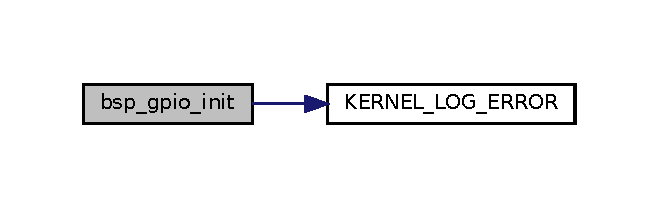
\includegraphics[width=316pt]{bsp__gpio_8c_ac05d93f29cf8cdcd3809298fe5df2f87_cgraph}
\end{center}
\end{figure}
Here is the caller graph for this function\+:\nopagebreak
\begin{figure}[H]
\begin{center}
\leavevmode
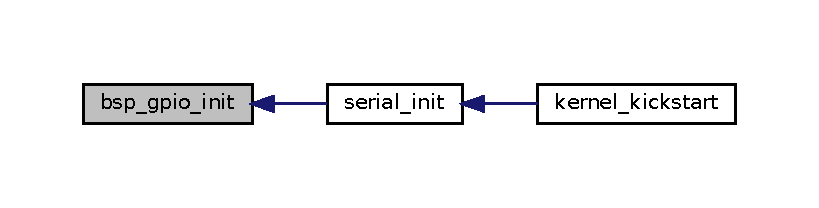
\includegraphics[width=350pt]{bsp__gpio_8c_ac05d93f29cf8cdcd3809298fe5df2f87_icgraph}
\end{center}
\end{figure}

\hypertarget{bsp__power_8c}{}\section{Kernel/\+Sources/arch/board/stm32/f401re/src/bsp\+\_\+power.c File Reference}
\label{bsp__power_8c}\index{Kernel/\+Sources/arch/board/stm32/f401re/src/bsp\+\_\+power.\+c@{Kernel/\+Sources/arch/board/stm32/f401re/src/bsp\+\_\+power.\+c}}
{\ttfamily \#include \char`\"{}error\+\_\+types.\+h\char`\"{}}\newline
{\ttfamily \#include \char`\"{}bsp\+\_\+power.\+h\char`\"{}}\newline
{\ttfamily \#include \char`\"{}stdint.\+h\char`\"{}}\newline
{\ttfamily \#include \char`\"{}config.\+h\char`\"{}}\newline
Include dependency graph for bsp\+\_\+power.\+c\+:\nopagebreak
\begin{figure}[H]
\begin{center}
\leavevmode
\includegraphics[width=337pt]{bsp__power_8c__incl}
\end{center}
\end{figure}
\subsection*{Functions}
\begin{DoxyCompactItemize}
\item 
\hyperlink{error__types_8h_acf146bc98f60f47c79d782f7523e339c}{E\+R\+R\+O\+R\+\_\+\+C\+O\+D\+E\+\_\+E} \hyperlink{bsp__power_8c_abe4bd68d683c1ab3fbc83afb60b36ede}{bsp\+\_\+pwr\+\_\+set\+\_\+scaling} (const \hyperlink{bsp__power_8h_adbcdf5dee7695e72280aa56c141f5758}{P\+O\+W\+E\+R\+\_\+\+S\+C\+A\+L\+I\+N\+G\+\_\+E} pwr\+\_\+scaling)
\begin{DoxyCompactList}\small\item\em Sets the power scaling. \end{DoxyCompactList}\end{DoxyCompactItemize}


\subsection{Function Documentation}
\mbox{\Hypertarget{bsp__power_8c_abe4bd68d683c1ab3fbc83afb60b36ede}\label{bsp__power_8c_abe4bd68d683c1ab3fbc83afb60b36ede}} 
\index{bsp\+\_\+power.\+c@{bsp\+\_\+power.\+c}!bsp\+\_\+pwr\+\_\+set\+\_\+scaling@{bsp\+\_\+pwr\+\_\+set\+\_\+scaling}}
\index{bsp\+\_\+pwr\+\_\+set\+\_\+scaling@{bsp\+\_\+pwr\+\_\+set\+\_\+scaling}!bsp\+\_\+power.\+c@{bsp\+\_\+power.\+c}}
\subsubsection{\texorpdfstring{bsp\+\_\+pwr\+\_\+set\+\_\+scaling()}{bsp\_pwr\_set\_scaling()}}
{\footnotesize\ttfamily \hyperlink{error__types_8h_acf146bc98f60f47c79d782f7523e339c}{E\+R\+R\+O\+R\+\_\+\+C\+O\+D\+E\+\_\+E} bsp\+\_\+pwr\+\_\+set\+\_\+scaling (\begin{DoxyParamCaption}\item[{const \hyperlink{bsp__power_8h_adbcdf5dee7695e72280aa56c141f5758}{P\+O\+W\+E\+R\+\_\+\+S\+C\+A\+L\+I\+N\+G\+\_\+E}}]{pwr\+\_\+scaling }\end{DoxyParamCaption})}



Sets the power scaling. 

Sets the power scaling based on the values passed in paramter. The scaling conforms to the values defined by the reference manual. If the value does not conform, the function has no effect and returns an error code.


\begin{DoxyParams}{Parameters}
{\em pwr\+\_\+scaling} & The scaling factor configuration.\\
\hline
\end{DoxyParams}
\begin{DoxyReturn}{Returns}
N\+O\+\_\+\+E\+R\+R\+OR is returned in case of success. Otherwise an error code is returned. Please refer to the list of the standard error codes. 
\end{DoxyReturn}


Definition at line 33 of file bsp\+\_\+power.\+c.


\begin{DoxyCode}
34 \{
35     \textcolor{comment}{/* Sets the power scaling value, we don't apply mask verification because 
}
36 \textcolor{comment}{     * the POWER\_SCALING\_E enumeration should already contain the right values.
}
37 \textcolor{comment}{     */}
38     *\hyperlink{bsp__power_8h_a30eb4f51898e3d42222ed18e4f392156}{PWR\_CR\_REGISTER} = (*\hyperlink{bsp__power_8h_a30eb4f51898e3d42222ed18e4f392156}{PWR\_CR\_REGISTER} & ~
      \hyperlink{bsp__power_8h_a06db718126d979cbf61fc27991514e1a}{PWR\_CR\_VOS\_MASK}) | pwr\_scaling;
39 
40     \textcolor{comment}{/* Delay to ensure bit update */}
41     \textcolor{keywordflow}{while}((*\hyperlink{bsp__power_8h_a30eb4f51898e3d42222ed18e4f392156}{PWR\_CR\_REGISTER} & \hyperlink{bsp__power_8h_a06db718126d979cbf61fc27991514e1a}{PWR\_CR\_VOS\_MASK}) != pwr\_scaling);
42 
43 \textcolor{preprocessor}{#if KERNEL\_LOG\_LEVEL >= INFO\_LOG\_LEVEL
}
44     KERNEL\_LOG\_INFO(\textcolor{stringliteral}{"Power scaling mode changed"}, 
45                     pwr\_scaling, 
46                     \textcolor{keyword}{sizeof}(pwr\_scaling), 
47                     \hyperlink{error__types_8h_a4db9ee29f2ff83c71567c12f6bfbf28cabf350750d0d4fabd8954c0f1e9bbae94}{NO\_ERROR});
48 \textcolor{preprocessor}{#endif
}
49 
50     \textcolor{keywordflow}{return} \hyperlink{error__types_8h_a4db9ee29f2ff83c71567c12f6bfbf28cabf350750d0d4fabd8954c0f1e9bbae94}{NO\_ERROR};
51 \}
\end{DoxyCode}
Here is the caller graph for this function\+:\nopagebreak
\begin{figure}[H]
\begin{center}
\leavevmode
\includegraphics[width=329pt]{bsp__power_8c_abe4bd68d683c1ab3fbc83afb60b36ede_icgraph}
\end{center}
\end{figure}

\hypertarget{bsp__usart_8c}{}\section{Kernel/\+Sources/arch/board/stm32/f401re/src/bsp\+\_\+usart.c File Reference}
\label{bsp__usart_8c}\index{Kernel/\+Sources/arch/board/stm32/f401re/src/bsp\+\_\+usart.\+c@{Kernel/\+Sources/arch/board/stm32/f401re/src/bsp\+\_\+usart.\+c}}
{\ttfamily \#include \char`\"{}error\+\_\+types.\+h\char`\"{}}\newline
{\ttfamily \#include \char`\"{}bsp\+\_\+usart.\+h\char`\"{}}\newline
{\ttfamily \#include \char`\"{}bsp\+\_\+clocks.\+h\char`\"{}}\newline
{\ttfamily \#include \char`\"{}serial.\+h\char`\"{}}\newline
{\ttfamily \#include \char`\"{}config.\+h\char`\"{}}\newline
{\ttfamily \#include \char`\"{}stddef.\+h\char`\"{}}\newline
{\ttfamily \#include \char`\"{}logger.\+h\char`\"{}}\newline
Include dependency graph for bsp\+\_\+usart.\+c\+:\nopagebreak
\begin{figure}[H]
\begin{center}
\leavevmode
\includegraphics[width=350pt]{bsp__usart_8c__incl}
\end{center}
\end{figure}
\subsection*{Macros}
\begin{DoxyCompactItemize}
\item 
\#define \hyperlink{bsp__usart_8c_a8aa979774d50a01cae417a899595055c}{C\+H\+E\+C\+K\+\_\+\+B\+A\+U\+D\+R\+A\+TE}(baudrate)
\begin{DoxyCompactList}\small\item\em Checks the baudrate setting conformity. \end{DoxyCompactList}\item 
\#define \hyperlink{bsp__usart_8c_a51885194f22c4bd5f94ab0bb253dd079}{C\+H\+E\+C\+K\+\_\+\+W\+D\+L\+E\+N\+G\+TH}(wdlength)
\begin{DoxyCompactList}\small\item\em Checks the word length setting conformity. \end{DoxyCompactList}\item 
\#define \hyperlink{bsp__usart_8c_ace359bfb3e864f995667f829a5520105}{C\+H\+E\+C\+K\+\_\+\+S\+T\+O\+P\+B\+I\+TS}(stpbits)
\begin{DoxyCompactList}\small\item\em Checks the stop bits setting conformity. \end{DoxyCompactList}\item 
\#define \hyperlink{bsp__usart_8c_a2c164787cf0d531b3c026aa2b9193a2b}{C\+H\+E\+C\+K\+\_\+\+P\+A\+R\+I\+T\+Y\+VA}(parity)
\begin{DoxyCompactList}\small\item\em Checks the parity setting conformity. \end{DoxyCompactList}\item 
\#define \hyperlink{bsp__usart_8c_a47ca255399a13357557641c6af83af64}{C\+H\+E\+C\+K\+\_\+\+C\+T\+R\+L\+F\+L\+OW}(ctrlflow)
\begin{DoxyCompactList}\small\item\em Checks the flow control setting conformity. \end{DoxyCompactList}\item 
\#define \hyperlink{bsp__usart_8c_a3fb76e1ecccca1505a00f7cbf6cbe2d2}{U\+S\+A\+R\+T\+\_\+\+G\+E\+T\+\_\+\+B\+R\+R\+\_\+\+D\+I\+V\+\_\+\+M\+A\+N\+T\+\_\+16}(f,  b)~((\hyperlink{stdint_8h_aaa5d1cd013383c889537491c3cfd9aad}{uint64\+\_\+t})f / ((\hyperlink{stdint_8h_aaa5d1cd013383c889537491c3cfd9aad}{uint64\+\_\+t})16 $\ast$ (\hyperlink{stdint_8h_aaa5d1cd013383c889537491c3cfd9aad}{uint64\+\_\+t})b))
\begin{DoxyCompactList}\small\item\em Compute the B\+RR bivider mantissa for a 16 bit oversampling. \end{DoxyCompactList}\item 
\#define \hyperlink{bsp__usart_8c_a34e3b693f024488a2a09c0b1c0f71f96}{U\+S\+A\+R\+T\+\_\+\+G\+E\+T\+\_\+\+B\+R\+R\+\_\+\+D\+I\+V\+\_\+\+F\+R\+A\+Q\+\_\+16}(f,  b)
\begin{DoxyCompactList}\small\item\em Compute the B\+RR bivider fraction for a 16 bit oversampling. \end{DoxyCompactList}\end{DoxyCompactItemize}
\subsection*{Functions}
\begin{DoxyCompactItemize}
\item 
void \hyperlink{bsp__usart_8c_a39d14fff7f007d639de7a6db12fd8acf}{bsp\+\_\+uart\+\_\+init} (const \hyperlink{bsp__usart_8h_a594f9d90a9a3875660da4512fb208cf9}{U\+S\+A\+R\+T\+\_\+\+I\+D\+E\+N\+T\+I\+F\+I\+E\+R\+\_\+E} usart\+\_\+id, const \hyperlink{serial_8h_acf007a933480ae3b580e6bccdc4b7c40}{S\+E\+R\+I\+A\+L\+\_\+\+S\+E\+T\+T\+I\+N\+G\+S\+\_\+T} $\ast$settings)
\begin{DoxyCompactList}\small\item\em Initializes the U\+S\+A\+RT as U\+A\+RT. \end{DoxyCompactList}\item 
void \hyperlink{bsp__usart_8c_a81aa58ca3b3ff2a16c5666f1601dedc7}{bsp\+\_\+usart\+\_\+disable} (const \hyperlink{bsp__usart_8h_a594f9d90a9a3875660da4512fb208cf9}{U\+S\+A\+R\+T\+\_\+\+I\+D\+E\+N\+T\+I\+F\+I\+E\+R\+\_\+E} usart\+\_\+id)
\begin{DoxyCompactList}\small\item\em Disables the U\+S\+A\+RT. \end{DoxyCompactList}\item 
void \hyperlink{bsp__usart_8c_ae71596fd1683989728deee59105b9b06}{bsp\+\_\+usart\+\_\+enable} (const \hyperlink{bsp__usart_8h_a594f9d90a9a3875660da4512fb208cf9}{U\+S\+A\+R\+T\+\_\+\+I\+D\+E\+N\+T\+I\+F\+I\+E\+R\+\_\+E} usart\+\_\+id)
\begin{DoxyCompactList}\small\item\em Enables the U\+S\+A\+RT. \end{DoxyCompactList}\item 
\hyperlink{error__types_8h_acf146bc98f60f47c79d782f7523e339c}{E\+R\+R\+O\+R\+\_\+\+C\+O\+D\+E\+\_\+E} \hyperlink{bsp__usart_8c_ac8063a6773891c77be25ad972f915f35}{serial\+\_\+init} (const \hyperlink{serial_8h_acf007a933480ae3b580e6bccdc4b7c40}{S\+E\+R\+I\+A\+L\+\_\+\+S\+E\+T\+T\+I\+N\+G\+S\+\_\+T} $\ast$settings)
\begin{DoxyCompactList}\small\item\em Initializes the serial line. \end{DoxyCompactList}\item 
\hyperlink{error__types_8h_acf146bc98f60f47c79d782f7523e339c}{E\+R\+R\+O\+R\+\_\+\+C\+O\+D\+E\+\_\+E} \hyperlink{bsp__usart_8c_a28c404f87f73ce3d02c889d4792d6a19}{serial\+\_\+write} (const char $\ast$str, const \hyperlink{stddef_8h_aa9d55e2f20e580b7445617d0d12fff6e}{size\+\_\+t} length)
\begin{DoxyCompactList}\small\item\em Writes a string of characters to the serial line. \end{DoxyCompactList}\end{DoxyCompactItemize}
\subsection*{Variables}
\begin{DoxyCompactItemize}
\item 
\hyperlink{stdint_8h_aba7bc1797add20fe3efdf37ced1182c5}{uint8\+\_\+t} \hyperlink{bsp__usart_8c_ad317e99f056e9ce535815fcdd1697c93}{usart\+\_\+init\+\_\+state} = 0
\begin{DoxyCompactList}\small\item\em Current usart initialization state. \end{DoxyCompactList}\end{DoxyCompactItemize}


\subsection{Macro Definition Documentation}
\mbox{\Hypertarget{bsp__usart_8c_a8aa979774d50a01cae417a899595055c}\label{bsp__usart_8c_a8aa979774d50a01cae417a899595055c}} 
\index{bsp\+\_\+usart.\+c@{bsp\+\_\+usart.\+c}!C\+H\+E\+C\+K\+\_\+\+B\+A\+U\+D\+R\+A\+TE@{C\+H\+E\+C\+K\+\_\+\+B\+A\+U\+D\+R\+A\+TE}}
\index{C\+H\+E\+C\+K\+\_\+\+B\+A\+U\+D\+R\+A\+TE@{C\+H\+E\+C\+K\+\_\+\+B\+A\+U\+D\+R\+A\+TE}!bsp\+\_\+usart.\+c@{bsp\+\_\+usart.\+c}}
\subsubsection{\texorpdfstring{C\+H\+E\+C\+K\+\_\+\+B\+A\+U\+D\+R\+A\+TE}{CHECK\_BAUDRATE}}
{\footnotesize\ttfamily \#define C\+H\+E\+C\+K\+\_\+\+B\+A\+U\+D\+R\+A\+TE(\begin{DoxyParamCaption}\item[{}]{baudrate }\end{DoxyParamCaption})}

{\bfseries Value\+:}
\begin{DoxyCode}
(\{                                                          \(\backslash\)
    switch(baudrate)                                        \(\backslash\)
    \{                                                       \(\backslash\)
        case 1200:                                          \(\backslash\)
        case 2400:                                          \(\backslash\)
        case 9600:                                          \(\backslash\)
        case 19200:                                         \(\backslash\)
        case 38400:                                         \(\backslash\)
        case 57600:                                         \(\backslash\)
        case 115200:                                        \(\backslash\)
        case 256000:                                        \(\backslash\)
        case 460800:                                        \(\backslash\)
        case 921600:                                        \(\backslash\)
        case 1843200:                                       \(\backslash\)
            break;                                          \(\backslash\)
        default:                                            \(\backslash\)
            if(\hyperlink{config_8h_a6c272d2b12ffba9bdd5a4d5dd608a0f8}{KERNEL\_LOG\_LEVEL} == \hyperlink{config_8h_a023f94f341f2300adee0891b15b364b2}{ERROR\_LOG\_LEVEL})         \(\backslash\)
            \{                                               \(\backslash\)
                KERNEL\_LOG\_ERROR(\textcolor{stringliteral}{"Invalid USART baudrate"},  \(\backslash\)
                                 (\textcolor{keywordtype}{void}*)baudrate,           \(\backslash\)
                                 \textcolor{keyword}{sizeof}(baudrate),          \(\backslash\)
                                 \hyperlink{error__types_8h_a4db9ee29f2ff83c71567c12f6bfbf28cabbe6797281350f36c23d07d6f2d7f6e2}{ERROR\_INVALID\_PARAM});      \(\backslash\)
            \}                                               \(\backslash\)
                                                            \(\backslash\)
            return \hyperlink{error__types_8h_a4db9ee29f2ff83c71567c12f6bfbf28cabbe6797281350f36c23d07d6f2d7f6e2}{ERROR\_INVALID\_PARAM};                     \(\backslash\)
                                                            \(\backslash\)
    \}                                                       \(\backslash\)
\})
\end{DoxyCode}


Checks the baudrate setting conformity. 

This macro will return from the function it is used in if an error is detected. An error message will be logged and an invalid parameter error is returned.


\begin{DoxyParams}[1]{Parameters}
\mbox{\tt in}  & {\em baudrate} & The baudrate settings for the serial line. \\
\hline
\end{DoxyParams}


Definition at line 46 of file bsp\+\_\+usart.\+c.

\mbox{\Hypertarget{bsp__usart_8c_a47ca255399a13357557641c6af83af64}\label{bsp__usart_8c_a47ca255399a13357557641c6af83af64}} 
\index{bsp\+\_\+usart.\+c@{bsp\+\_\+usart.\+c}!C\+H\+E\+C\+K\+\_\+\+C\+T\+R\+L\+F\+L\+OW@{C\+H\+E\+C\+K\+\_\+\+C\+T\+R\+L\+F\+L\+OW}}
\index{C\+H\+E\+C\+K\+\_\+\+C\+T\+R\+L\+F\+L\+OW@{C\+H\+E\+C\+K\+\_\+\+C\+T\+R\+L\+F\+L\+OW}!bsp\+\_\+usart.\+c@{bsp\+\_\+usart.\+c}}
\subsubsection{\texorpdfstring{C\+H\+E\+C\+K\+\_\+\+C\+T\+R\+L\+F\+L\+OW}{CHECK\_CTRLFLOW}}
{\footnotesize\ttfamily \#define C\+H\+E\+C\+K\+\_\+\+C\+T\+R\+L\+F\+L\+OW(\begin{DoxyParamCaption}\item[{}]{ctrlflow }\end{DoxyParamCaption})}

{\bfseries Value\+:}
\begin{DoxyCode}
(\{                                                             \(\backslash\)
    switch(ctrlflow)                                           \(\backslash\)
    \{                                                          \(\backslash\)
        case \hyperlink{serial_8h_ab85f99523d332a127bd78d8fd075e9f4}{SERIAL\_CTRL\_FLOW\_NONE}:                            \(\backslash\)
        case \hyperlink{serial_8h_a0d44b3d3d3e5bb25dc7b976dc2acd4d6}{SERIAL\_CTRL\_FLOW\_CTS}:                             \(\backslash\)
        case \hyperlink{serial_8h_a2335857b5c95b76430e052c05f6e71b5}{SERIAL\_CTRL\_FLOW\_RTS}:                             \(\backslash\)
        case \hyperlink{serial_8h_a5eadb2a7b63f2b5483b5c4aed197d99a}{SERIAL\_CTRL\_FLOW\_CTS\_RTS}:                         \(\backslash\)
            break;                                             \(\backslash\)
        default:                                               \(\backslash\)
            if(\hyperlink{config_8h_a6c272d2b12ffba9bdd5a4d5dd608a0f8}{KERNEL\_LOG\_LEVEL} == \hyperlink{config_8h_a023f94f341f2300adee0891b15b364b2}{ERROR\_LOG\_LEVEL})            \(\backslash\)
            \{                                                  \(\backslash\)
                KERNEL\_LOG\_ERROR(\textcolor{stringliteral}{"Invalid USART control flow"}, \(\backslash\)
                                 (\textcolor{keywordtype}{void}*)(\hyperlink{stdint_8h_a324c5d28c0d82f502a234ab99efac87a}{uint32\_t})ctrlflow,    \(\backslash\)
                                 \textcolor{keyword}{sizeof}(ctrlflow),             \(\backslash\)
                                 \hyperlink{error__types_8h_a4db9ee29f2ff83c71567c12f6bfbf28cabbe6797281350f36c23d07d6f2d7f6e2}{ERROR\_INVALID\_PARAM});         \(\backslash\)
            \}                                                  \(\backslash\)
                                                               \(\backslash\)
            return \hyperlink{error__types_8h_a4db9ee29f2ff83c71567c12f6bfbf28cabbe6797281350f36c23d07d6f2d7f6e2}{ERROR\_INVALID\_PARAM};                        \(\backslash\)
                                                               \(\backslash\)
    \}                                                          \(\backslash\)
\})
\end{DoxyCode}


Checks the flow control setting conformity. 

This macro will return from the function it is used in if an error is detected. An error message will be logged and an invalid parameter error is returned.


\begin{DoxyParams}[1]{Parameters}
\mbox{\tt in}  & {\em ctrlflow} & The flow control for the serial line. \\
\hline
\end{DoxyParams}


Definition at line 178 of file bsp\+\_\+usart.\+c.

\mbox{\Hypertarget{bsp__usart_8c_a2c164787cf0d531b3c026aa2b9193a2b}\label{bsp__usart_8c_a2c164787cf0d531b3c026aa2b9193a2b}} 
\index{bsp\+\_\+usart.\+c@{bsp\+\_\+usart.\+c}!C\+H\+E\+C\+K\+\_\+\+P\+A\+R\+I\+T\+Y\+VA@{C\+H\+E\+C\+K\+\_\+\+P\+A\+R\+I\+T\+Y\+VA}}
\index{C\+H\+E\+C\+K\+\_\+\+P\+A\+R\+I\+T\+Y\+VA@{C\+H\+E\+C\+K\+\_\+\+P\+A\+R\+I\+T\+Y\+VA}!bsp\+\_\+usart.\+c@{bsp\+\_\+usart.\+c}}
\subsubsection{\texorpdfstring{C\+H\+E\+C\+K\+\_\+\+P\+A\+R\+I\+T\+Y\+VA}{CHECK\_PARITYVA}}
{\footnotesize\ttfamily \#define C\+H\+E\+C\+K\+\_\+\+P\+A\+R\+I\+T\+Y\+VA(\begin{DoxyParamCaption}\item[{}]{parity }\end{DoxyParamCaption})}

{\bfseries Value\+:}
\begin{DoxyCode}
(\{                                                             \(\backslash\)
    switch(parity)                                             \(\backslash\)
    \{                                                          \(\backslash\)
        case \hyperlink{serial_8h_ad3af92391cfd2670eb782a60c7f923a6}{SERIAL\_PARITY\_NONE}:                               \(\backslash\)
        case \hyperlink{serial_8h_ab1469484b1ad5e39561c21b5a590eaf6}{SERIAL\_PARITY\_EVEN}:                               \(\backslash\)
        case \hyperlink{serial_8h_aa1baeda93fe64b888113824d02471d0f}{SERIAL\_PARITY\_ODD}:                                \(\backslash\)
            break;                                             \(\backslash\)
        default:                                               \(\backslash\)
            if(\hyperlink{config_8h_a6c272d2b12ffba9bdd5a4d5dd608a0f8}{KERNEL\_LOG\_LEVEL} == \hyperlink{config_8h_a023f94f341f2300adee0891b15b364b2}{ERROR\_LOG\_LEVEL})            \(\backslash\)
            \{                                                  \(\backslash\)
                KERNEL\_LOG\_ERROR(\textcolor{stringliteral}{"Invalid USART partity mode"}, \(\backslash\)
                                 (\textcolor{keywordtype}{void}*)(\hyperlink{stdint_8h_a324c5d28c0d82f502a234ab99efac87a}{uint32\_t})parity,      \(\backslash\)
                                 \textcolor{keyword}{sizeof}(parity),               \(\backslash\)
                                 \hyperlink{error__types_8h_a4db9ee29f2ff83c71567c12f6bfbf28cabbe6797281350f36c23d07d6f2d7f6e2}{ERROR\_INVALID\_PARAM});         \(\backslash\)
            \}                                                  \(\backslash\)
                                                               \(\backslash\)
            return \hyperlink{error__types_8h_a4db9ee29f2ff83c71567c12f6bfbf28cabbe6797281350f36c23d07d6f2d7f6e2}{ERROR\_INVALID\_PARAM};                        \(\backslash\)
                                                               \(\backslash\)
    \}                                                          \(\backslash\)
\})
\end{DoxyCode}


Checks the parity setting conformity. 

This macro will return from the function it is used in if an error is detected. An error message will be logged and an invalid parameter error is returned.


\begin{DoxyParams}[1]{Parameters}
\mbox{\tt in}  & {\em parity} & The parity settings for the serial line. \\
\hline
\end{DoxyParams}


Definition at line 147 of file bsp\+\_\+usart.\+c.

\mbox{\Hypertarget{bsp__usart_8c_ace359bfb3e864f995667f829a5520105}\label{bsp__usart_8c_ace359bfb3e864f995667f829a5520105}} 
\index{bsp\+\_\+usart.\+c@{bsp\+\_\+usart.\+c}!C\+H\+E\+C\+K\+\_\+\+S\+T\+O\+P\+B\+I\+TS@{C\+H\+E\+C\+K\+\_\+\+S\+T\+O\+P\+B\+I\+TS}}
\index{C\+H\+E\+C\+K\+\_\+\+S\+T\+O\+P\+B\+I\+TS@{C\+H\+E\+C\+K\+\_\+\+S\+T\+O\+P\+B\+I\+TS}!bsp\+\_\+usart.\+c@{bsp\+\_\+usart.\+c}}
\subsubsection{\texorpdfstring{C\+H\+E\+C\+K\+\_\+\+S\+T\+O\+P\+B\+I\+TS}{CHECK\_STOPBITS}}
{\footnotesize\ttfamily \#define C\+H\+E\+C\+K\+\_\+\+S\+T\+O\+P\+B\+I\+TS(\begin{DoxyParamCaption}\item[{}]{stpbits }\end{DoxyParamCaption})}

{\bfseries Value\+:}
\begin{DoxyCode}
(\{                                                             \(\backslash\)
    switch(stpbits)                                            \(\backslash\)
    \{                                                          \(\backslash\)
        case \hyperlink{serial_8h_a53a4c884223db0ce40e97ed0cc5e6d19}{SERIAL\_STOP\_BITS\_05}:                              \(\backslash\)
        case \hyperlink{serial_8h_a2b63bfe663eaa7e96165898d0bad9ba1}{SERIAL\_STOP\_BITS\_1}:                               \(\backslash\)
        case \hyperlink{serial_8h_adfe27b7a5b350830ec68973c5aa7de7a}{SERIAL\_STOP\_BITS\_15}:                              \(\backslash\)
        case \hyperlink{serial_8h_ad91c5a26785732ceabc6feddf28a2695}{SERIAL\_STOP\_BITS\_2}:                               \(\backslash\)
            break;                                             \(\backslash\)
        default:                                               \(\backslash\)
            if(\hyperlink{config_8h_a6c272d2b12ffba9bdd5a4d5dd608a0f8}{KERNEL\_LOG\_LEVEL} == \hyperlink{config_8h_a023f94f341f2300adee0891b15b364b2}{ERROR\_LOG\_LEVEL})            \(\backslash\)
            \{                                                  \(\backslash\)
                KERNEL\_LOG\_ERROR(\textcolor{stringliteral}{"Invalid USART stop bits"},    \(\backslash\)
                                 (\textcolor{keywordtype}{void}*)(\hyperlink{stdint_8h_a324c5d28c0d82f502a234ab99efac87a}{uint32\_t})stpbits,     \(\backslash\)
                                 \textcolor{keyword}{sizeof}(stpbits),              \(\backslash\)
                                 \hyperlink{error__types_8h_a4db9ee29f2ff83c71567c12f6bfbf28cabbe6797281350f36c23d07d6f2d7f6e2}{ERROR\_INVALID\_PARAM});         \(\backslash\)
            \}                                                  \(\backslash\)
                                                               \(\backslash\)
            return \hyperlink{error__types_8h_a4db9ee29f2ff83c71567c12f6bfbf28cabbe6797281350f36c23d07d6f2d7f6e2}{ERROR\_INVALID\_PARAM};                        \(\backslash\)
                                                               \(\backslash\)
    \}                                                          \(\backslash\)
\})
\end{DoxyCode}


Checks the stop bits setting conformity. 

This macro will return from the function it is used in if an error is detected. An error message will be logged and an invalid parameter error is returned.


\begin{DoxyParams}[1]{Parameters}
\mbox{\tt in}  & {\em stpbits} & The stop bits settings for the serial line. \\
\hline
\end{DoxyParams}


Definition at line 115 of file bsp\+\_\+usart.\+c.

\mbox{\Hypertarget{bsp__usart_8c_a51885194f22c4bd5f94ab0bb253dd079}\label{bsp__usart_8c_a51885194f22c4bd5f94ab0bb253dd079}} 
\index{bsp\+\_\+usart.\+c@{bsp\+\_\+usart.\+c}!C\+H\+E\+C\+K\+\_\+\+W\+D\+L\+E\+N\+G\+TH@{C\+H\+E\+C\+K\+\_\+\+W\+D\+L\+E\+N\+G\+TH}}
\index{C\+H\+E\+C\+K\+\_\+\+W\+D\+L\+E\+N\+G\+TH@{C\+H\+E\+C\+K\+\_\+\+W\+D\+L\+E\+N\+G\+TH}!bsp\+\_\+usart.\+c@{bsp\+\_\+usart.\+c}}
\subsubsection{\texorpdfstring{C\+H\+E\+C\+K\+\_\+\+W\+D\+L\+E\+N\+G\+TH}{CHECK\_WDLENGTH}}
{\footnotesize\ttfamily \#define C\+H\+E\+C\+K\+\_\+\+W\+D\+L\+E\+N\+G\+TH(\begin{DoxyParamCaption}\item[{}]{wdlength }\end{DoxyParamCaption})}

{\bfseries Value\+:}
\begin{DoxyCode}
(\{                                                             \(\backslash\)
    switch(wdlength)                                           \(\backslash\)
    \{                                                          \(\backslash\)
        case 8:                                                \(\backslash\)
        case 9:                                                \(\backslash\)
            break;                                             \(\backslash\)
        default:                                               \(\backslash\)
            if(\hyperlink{config_8h_a6c272d2b12ffba9bdd5a4d5dd608a0f8}{KERNEL\_LOG\_LEVEL} == \hyperlink{config_8h_a023f94f341f2300adee0891b15b364b2}{ERROR\_LOG\_LEVEL})            \(\backslash\)
            \{                                                  \(\backslash\)
                KERNEL\_LOG\_ERROR(\textcolor{stringliteral}{"Invalid USART word length"},  \(\backslash\)
                                 (\textcolor{keywordtype}{void}*)(\hyperlink{stdint_8h_a324c5d28c0d82f502a234ab99efac87a}{uint32\_t})wdlength,    \(\backslash\)
                                 \textcolor{keyword}{sizeof}(wdlength),             \(\backslash\)
                                 \hyperlink{error__types_8h_a4db9ee29f2ff83c71567c12f6bfbf28cabbe6797281350f36c23d07d6f2d7f6e2}{ERROR\_INVALID\_PARAM});         \(\backslash\)
            \}                                                  \(\backslash\)
                                                               \(\backslash\)
            return \hyperlink{error__types_8h_a4db9ee29f2ff83c71567c12f6bfbf28cabbe6797281350f36c23d07d6f2d7f6e2}{ERROR\_INVALID\_PARAM};                        \(\backslash\)
                                                               \(\backslash\)
    \}                                                          \(\backslash\)
\})
\end{DoxyCode}


Checks the word length setting conformity. 

This macro will return from the function it is used in if an error is detected. An error message will be logged and an invalid parameter error is returned.


\begin{DoxyParams}[1]{Parameters}
\mbox{\tt in}  & {\em wdlength} & The word length settings for the serial line. \\
\hline
\end{DoxyParams}


Definition at line 85 of file bsp\+\_\+usart.\+c.

\mbox{\Hypertarget{bsp__usart_8c_a34e3b693f024488a2a09c0b1c0f71f96}\label{bsp__usart_8c_a34e3b693f024488a2a09c0b1c0f71f96}} 
\index{bsp\+\_\+usart.\+c@{bsp\+\_\+usart.\+c}!U\+S\+A\+R\+T\+\_\+\+G\+E\+T\+\_\+\+B\+R\+R\+\_\+\+D\+I\+V\+\_\+\+F\+R\+A\+Q\+\_\+16@{U\+S\+A\+R\+T\+\_\+\+G\+E\+T\+\_\+\+B\+R\+R\+\_\+\+D\+I\+V\+\_\+\+F\+R\+A\+Q\+\_\+16}}
\index{U\+S\+A\+R\+T\+\_\+\+G\+E\+T\+\_\+\+B\+R\+R\+\_\+\+D\+I\+V\+\_\+\+F\+R\+A\+Q\+\_\+16@{U\+S\+A\+R\+T\+\_\+\+G\+E\+T\+\_\+\+B\+R\+R\+\_\+\+D\+I\+V\+\_\+\+F\+R\+A\+Q\+\_\+16}!bsp\+\_\+usart.\+c@{bsp\+\_\+usart.\+c}}
\subsubsection{\texorpdfstring{U\+S\+A\+R\+T\+\_\+\+G\+E\+T\+\_\+\+B\+R\+R\+\_\+\+D\+I\+V\+\_\+\+F\+R\+A\+Q\+\_\+16}{USART\_GET\_BRR\_DIV\_FRAQ\_16}}
{\footnotesize\ttfamily \#define U\+S\+A\+R\+T\+\_\+\+G\+E\+T\+\_\+\+B\+R\+R\+\_\+\+D\+I\+V\+\_\+\+F\+R\+A\+Q\+\_\+16(\begin{DoxyParamCaption}\item[{}]{f,  }\item[{}]{b }\end{DoxyParamCaption})}

{\bfseries Value\+:}
\begin{DoxyCode}
(((((\hyperlink{stdint_8h_aaa5d1cd013383c889537491c3cfd9aad}{uint64\_t})f * 100 / ((\hyperlink{stdint_8h_aaa5d1cd013383c889537491c3cfd9aad}{uint64\_t})16 * (\hyperlink{stdint_8h_aaa5d1cd013383c889537491c3cfd9aad}{uint64\_t})b)) -   \(\backslash\)
        (\hyperlink{bsp__usart_8c_a3fb76e1ecccca1505a00f7cbf6cbe2d2}{USART\_GET\_BRR\_DIV\_MANT\_16}(f, b) * 100)) * 16 + 50) / 100)
\end{DoxyCode}


Compute the B\+RR bivider fraction for a 16 bit oversampling. 


\begin{DoxyParams}[1]{Parameters}
\mbox{\tt in}  & {\em f} & The serial input clock frequency. \\
\hline
\mbox{\tt in}  & {\em b} & The required baudrate for the serial line.\\
\hline
\end{DoxyParams}
\begin{DoxyReturn}{Returns}
The B\+RR fraction is returned. 
\end{DoxyReturn}


Definition at line 220 of file bsp\+\_\+usart.\+c.

\mbox{\Hypertarget{bsp__usart_8c_a3fb76e1ecccca1505a00f7cbf6cbe2d2}\label{bsp__usart_8c_a3fb76e1ecccca1505a00f7cbf6cbe2d2}} 
\index{bsp\+\_\+usart.\+c@{bsp\+\_\+usart.\+c}!U\+S\+A\+R\+T\+\_\+\+G\+E\+T\+\_\+\+B\+R\+R\+\_\+\+D\+I\+V\+\_\+\+M\+A\+N\+T\+\_\+16@{U\+S\+A\+R\+T\+\_\+\+G\+E\+T\+\_\+\+B\+R\+R\+\_\+\+D\+I\+V\+\_\+\+M\+A\+N\+T\+\_\+16}}
\index{U\+S\+A\+R\+T\+\_\+\+G\+E\+T\+\_\+\+B\+R\+R\+\_\+\+D\+I\+V\+\_\+\+M\+A\+N\+T\+\_\+16@{U\+S\+A\+R\+T\+\_\+\+G\+E\+T\+\_\+\+B\+R\+R\+\_\+\+D\+I\+V\+\_\+\+M\+A\+N\+T\+\_\+16}!bsp\+\_\+usart.\+c@{bsp\+\_\+usart.\+c}}
\subsubsection{\texorpdfstring{U\+S\+A\+R\+T\+\_\+\+G\+E\+T\+\_\+\+B\+R\+R\+\_\+\+D\+I\+V\+\_\+\+M\+A\+N\+T\+\_\+16}{USART\_GET\_BRR\_DIV\_MANT\_16}}
{\footnotesize\ttfamily \#define U\+S\+A\+R\+T\+\_\+\+G\+E\+T\+\_\+\+B\+R\+R\+\_\+\+D\+I\+V\+\_\+\+M\+A\+N\+T\+\_\+16(\begin{DoxyParamCaption}\item[{}]{f,  }\item[{}]{b }\end{DoxyParamCaption})~((\hyperlink{stdint_8h_aaa5d1cd013383c889537491c3cfd9aad}{uint64\+\_\+t})f / ((\hyperlink{stdint_8h_aaa5d1cd013383c889537491c3cfd9aad}{uint64\+\_\+t})16 $\ast$ (\hyperlink{stdint_8h_aaa5d1cd013383c889537491c3cfd9aad}{uint64\+\_\+t})b))}



Compute the B\+RR bivider mantissa for a 16 bit oversampling. 


\begin{DoxyParams}[1]{Parameters}
\mbox{\tt in}  & {\em f} & The serial input clock frequency. \\
\hline
\mbox{\tt in}  & {\em b} & The required baudrate for the serial line.\\
\hline
\end{DoxyParams}
\begin{DoxyReturn}{Returns}
The B\+RR mantissa is returned. 
\end{DoxyReturn}


Definition at line 209 of file bsp\+\_\+usart.\+c.



\subsection{Function Documentation}
\mbox{\Hypertarget{bsp__usart_8c_a39d14fff7f007d639de7a6db12fd8acf}\label{bsp__usart_8c_a39d14fff7f007d639de7a6db12fd8acf}} 
\index{bsp\+\_\+usart.\+c@{bsp\+\_\+usart.\+c}!bsp\+\_\+uart\+\_\+init@{bsp\+\_\+uart\+\_\+init}}
\index{bsp\+\_\+uart\+\_\+init@{bsp\+\_\+uart\+\_\+init}!bsp\+\_\+usart.\+c@{bsp\+\_\+usart.\+c}}
\subsubsection{\texorpdfstring{bsp\+\_\+uart\+\_\+init()}{bsp\_uart\_init()}}
{\footnotesize\ttfamily void bsp\+\_\+uart\+\_\+init (\begin{DoxyParamCaption}\item[{const \hyperlink{bsp__usart_8h_a594f9d90a9a3875660da4512fb208cf9}{U\+S\+A\+R\+T\+\_\+\+I\+D\+E\+N\+T\+I\+F\+I\+E\+R\+\_\+E}}]{usart\+\_\+id,  }\item[{const \hyperlink{serial_8h_acf007a933480ae3b580e6bccdc4b7c40}{S\+E\+R\+I\+A\+L\+\_\+\+S\+E\+T\+T\+I\+N\+G\+S\+\_\+T} $\ast$}]{settings }\end{DoxyParamCaption})}



Initializes the U\+S\+A\+RT as U\+A\+RT. 

Initializes the U\+S\+A\+RT as U\+A\+RT with the corresponding settings given as parameter.


\begin{DoxyParams}[1]{Parameters}
\mbox{\tt in}  & {\em usart\+\_\+id} & The identifier of the U\+S\+A\+RT to initialize. \\
\hline
\mbox{\tt in}  & {\em settings} & The settings structure to use to initialize the U\+A\+RT. \\
\hline
\end{DoxyParams}


Definition at line 233 of file bsp\+\_\+usart.\+c.


\begin{DoxyCode}
235 \{
236     \textcolor{keyword}{volatile} \hyperlink{stdint_8h_a324c5d28c0d82f502a234ab99efac87a}{uint32\_t}* cr1;
237     \textcolor{keyword}{volatile} \hyperlink{stdint_8h_a324c5d28c0d82f502a234ab99efac87a}{uint32\_t}* cr2;
238     \textcolor{keyword}{volatile} \hyperlink{stdint_8h_a324c5d28c0d82f502a234ab99efac87a}{uint32\_t}* cr3;
239     \textcolor{keyword}{volatile} \hyperlink{stdint_8h_a324c5d28c0d82f502a234ab99efac87a}{uint32\_t}* brr;
240 
241     \hyperlink{stdint_8h_a324c5d28c0d82f502a234ab99efac87a}{uint32\_t} freq;
242 
243     \textcolor{keywordflow}{switch}(usart\_id)
244     \{
245         \textcolor{keywordflow}{case} \hyperlink{bsp__usart_8h_a58f9be3820e29e0fbf00e2466c3ee768a512d550c862eac9ad45d923508bb0f7d}{USART\_ID\_1}:
246             cr1 = (\textcolor{keyword}{volatile} \hyperlink{stdint_8h_a324c5d28c0d82f502a234ab99efac87a}{uint32\_t}*)\hyperlink{bsp__usart_8h_a7e3cbb9c3b7b3967719512ff9df7d632}{USART1\_CR1\_ADDRESS};
247             cr2 = (\textcolor{keyword}{volatile} \hyperlink{stdint_8h_a324c5d28c0d82f502a234ab99efac87a}{uint32\_t}*)\hyperlink{bsp__usart_8h_a5130cce25ab86fc32b7846b2dcbc9abf}{USART1\_CR2\_ADDRESS};
248             cr3 = (\textcolor{keyword}{volatile} \hyperlink{stdint_8h_a324c5d28c0d82f502a234ab99efac87a}{uint32\_t}*)\hyperlink{bsp__usart_8h_a04b5bd4552470522cddb75322bb9e4a1}{USART1\_CR3\_ADDRESS};
249             brr = (\textcolor{keyword}{volatile} \hyperlink{stdint_8h_a324c5d28c0d82f502a234ab99efac87a}{uint32\_t}*)\hyperlink{bsp__usart_8h_abcaf3524a9622c5cec6d5d70027c5d15}{USART1\_BRR\_ADDRESS};
250             \textcolor{keywordflow}{break};
251         \textcolor{keywordflow}{case} \hyperlink{bsp__usart_8h_a58f9be3820e29e0fbf00e2466c3ee768abb138542d801249fd01ec62c34f52cff}{USART\_ID\_2}:
252             cr1 = (\textcolor{keyword}{volatile} \hyperlink{stdint_8h_a324c5d28c0d82f502a234ab99efac87a}{uint32\_t}*)\hyperlink{bsp__usart_8h_a551a35cf294b360d96b14bac0aa81c28}{USART2\_CR1\_ADDRESS};
253             cr2 = (\textcolor{keyword}{volatile} \hyperlink{stdint_8h_a324c5d28c0d82f502a234ab99efac87a}{uint32\_t}*)\hyperlink{bsp__usart_8h_aa130d46de6c5714614654179f9b690ca}{USART2\_CR2\_ADDRESS};
254             cr3 = (\textcolor{keyword}{volatile} \hyperlink{stdint_8h_a324c5d28c0d82f502a234ab99efac87a}{uint32\_t}*)\hyperlink{bsp__usart_8h_a4aceb0927ac1c8ec7adad8e44a0d626a}{USART2\_CR3\_ADDRESS};
255             brr = (\textcolor{keyword}{volatile} \hyperlink{stdint_8h_a324c5d28c0d82f502a234ab99efac87a}{uint32\_t}*)\hyperlink{bsp__usart_8h_a02ff054c09f139a38369680f85c1b9e4}{USART2\_BRR\_ADDRESS};
256             \textcolor{keywordflow}{break};
257         \textcolor{keywordflow}{case} \hyperlink{bsp__usart_8h_a58f9be3820e29e0fbf00e2466c3ee768afd45e5de3678cbcada70f46bde327479}{USART\_ID\_6}:
258             cr1 = (\textcolor{keyword}{volatile} \hyperlink{stdint_8h_a324c5d28c0d82f502a234ab99efac87a}{uint32\_t}*)\hyperlink{bsp__usart_8h_a52e23572285d44dea63aff07039d248e}{USART6\_CR1\_ADDRESS};
259             cr2 = (\textcolor{keyword}{volatile} \hyperlink{stdint_8h_a324c5d28c0d82f502a234ab99efac87a}{uint32\_t}*)\hyperlink{bsp__usart_8h_a94170d0ce631976cd1daefcb320a1815}{USART6\_CR2\_ADDRESS};
260             cr3 = (\textcolor{keyword}{volatile} \hyperlink{stdint_8h_a324c5d28c0d82f502a234ab99efac87a}{uint32\_t}*)\hyperlink{bsp__usart_8h_aa5de805e5b75dd00bb77531e7273ad14}{USART6\_CR3\_ADDRESS};
261             brr = (\textcolor{keyword}{volatile} \hyperlink{stdint_8h_a324c5d28c0d82f502a234ab99efac87a}{uint32\_t}*)\hyperlink{bsp__usart_8h_a8089788317790f6633511039cb7d50b8}{USART6\_BRR\_ADDRESS};
262             \textcolor{keywordflow}{break};
263         \textcolor{keywordflow}{default}:
264             \textcolor{keywordflow}{return};
265     \}
266 
267     \textcolor{comment}{/* Set CR1 register */}
268     *cr1 = *cr1 & ~(\hyperlink{bsp__usart_8h_aed6caeb0cb48f1a7b34090f31a92a8e2}{USART\_CR1\_OVER8}  | \hyperlink{bsp__usart_8h_a95f0288b9c6aaeca7cb6550a2e6833e2}{USART\_CR1\_M}      | 
269                     \hyperlink{bsp__usart_8h_ad831dfc169fcf14b7284984dbecf322d}{USART\_CR1\_WAKE}   | \hyperlink{bsp__usart_8h_a60f8fcf084f9a8514efafb617c70b074}{USART\_CR1\_PCE}    |
270                     \hyperlink{bsp__usart_8h_a2e159d36ab2c93a2c1942df60e9eebbe}{USART\_CR1\_PS}     | \hyperlink{bsp__usart_8h_a27405d413b6d355ccdb076d52fef6875}{USART\_CR1\_PEIE}   | 
271                     \hyperlink{bsp__usart_8h_a70422871d15f974b464365e7fe1877e9}{USART\_CR1\_TXEIE}  | \hyperlink{bsp__usart_8h_aa17130690a1ca95b972429eb64d4254e}{USART\_CR1\_TCIE}   | 
272                     \hyperlink{bsp__usart_8h_a91118f867adfdb2e805beea86666de04}{USART\_CR1\_RXNEIE} | \hyperlink{bsp__usart_8h_a5221d09eebd12445a20f221bf98066f8}{USART\_CR1\_IDLEIE} | 
273                     \hyperlink{bsp__usart_8h_ade7f090b04fd78b755b43357ecaa9622}{USART\_CR1\_TE}     | \hyperlink{bsp__usart_8h_ada0d5d407a22264de847bc1b40a17aeb}{USART\_CR1\_RE}     |
274                     \hyperlink{bsp__usart_8h_aa7d61ab5a4e2beaa3f591c56bd15a27b}{USART\_CR1\_RWU}    | \hyperlink{bsp__usart_8h_ac457c519baa28359ab7959fbe0c5cda1}{USART\_CR1\_SBK});
275 
276     *cr1 = *cr1 | 
277            (settings->\hyperlink{struct_s_e_r_i_a_l___s_e_t_t_i_n_g_s_ae9ff0fba282a81e6b05a1082ab54e14d}{word\_length} == 8 ? 0 : \hyperlink{bsp__usart_8h_a95f0288b9c6aaeca7cb6550a2e6833e2}{USART\_CR1\_M}) |
278            ((settings->\hyperlink{struct_s_e_r_i_a_l___s_e_t_t_i_n_g_s_a57fc780fe7a58343cb0513fd873e95fb}{partity} == \hyperlink{serial_8h_ab1469484b1ad5e39561c21b5a590eaf6}{SERIAL\_PARITY\_EVEN}) || 
279             (settings->\hyperlink{struct_s_e_r_i_a_l___s_e_t_t_i_n_g_s_a57fc780fe7a58343cb0513fd873e95fb}{partity} == \hyperlink{serial_8h_ad3af92391cfd2670eb782a60c7f923a6}{SERIAL\_PARITY\_NONE}) ? 0 : 
      \hyperlink{bsp__usart_8h_a2e159d36ab2c93a2c1942df60e9eebbe}{USART\_CR1\_PS}) |
280            (settings->\hyperlink{struct_s_e_r_i_a_l___s_e_t_t_i_n_g_s_a57fc780fe7a58343cb0513fd873e95fb}{partity} == \hyperlink{serial_8h_ad3af92391cfd2670eb782a60c7f923a6}{SERIAL\_PARITY\_NONE}   ? 0 : 
      \hyperlink{bsp__usart_8h_a60f8fcf084f9a8514efafb617c70b074}{USART\_CR1\_PCE}) |
281            \hyperlink{bsp__usart_8h_ade7f090b04fd78b755b43357ecaa9622}{USART\_CR1\_TE} | \hyperlink{bsp__usart_8h_ada0d5d407a22264de847bc1b40a17aeb}{USART\_CR1\_RE};
282 
283     \textcolor{comment}{/* Set CR2 register */}
284     *cr2 = *cr2 & ~(\hyperlink{bsp__usart_8h_ac8931efa62c29d92f5c0ec5a05f907ef}{USART\_CR2\_LINEN}     | \hyperlink{bsp__usart_8h_ae20ff98868e1e2fec55f2141b5a353bd}{USART\_CR2\_STOP\_MASK} | 
285                     \hyperlink{bsp__usart_8h_a42a396cde02ffa0c4d3fd9817b6af853}{USART\_CR2\_CLKEN}     | \hyperlink{bsp__usart_8h_afbb4336ac93d94d4e78f9fb7b3a0dc68}{USART\_CR2\_CPOL}      |
286                     \hyperlink{bsp__usart_8h_a362976ce813e58310399d113d2cf09cb}{USART\_CR2\_CPHA}      | \hyperlink{bsp__usart_8h_a4a62e93ae7864e89622bdd92508b615e}{USART\_CR2\_LBCL}      | 
287                     \hyperlink{bsp__usart_8h_af98769bed28dfd2b222e6884e464f9d2}{USART\_CR2\_LBIE}      | \hyperlink{bsp__usart_8h_a539ea2e20b534b2c742e3194f2ad5a5c}{USART\_CR2\_LBL}       | 
288                     \hyperlink{bsp__usart_8h_a8abd4cdca00f61296bc3a84a59992dd3}{USART\_CR2\_ADDR\_MASK});
289 
290     \textcolor{keywordflow}{switch}(settings->\hyperlink{struct_s_e_r_i_a_l___s_e_t_t_i_n_g_s_ae847d8b7e1095e0ae8d6eb1e4a281585}{stop\_bits})
291     \{
292         \textcolor{keywordflow}{case} \hyperlink{serial_8h_a53a4c884223db0ce40e97ed0cc5e6d19}{SERIAL\_STOP\_BITS\_05}:
293             *cr2 = *cr2 | \hyperlink{bsp__usart_8h_a41e7bdb66e99fb64359cd105d624d41c}{USART\_CR2\_STOP\_05};
294             \textcolor{keywordflow}{break};
295         \textcolor{keywordflow}{case} \hyperlink{serial_8h_adfe27b7a5b350830ec68973c5aa7de7a}{SERIAL\_STOP\_BITS\_15}:
296             *cr2 = *cr2 | \hyperlink{bsp__usart_8h_a57f01ae62391c4e1f82e899d8f765858}{USART\_CR2\_STOP\_15};
297             \textcolor{keywordflow}{break};
298         \textcolor{keywordflow}{case} \hyperlink{serial_8h_ad91c5a26785732ceabc6feddf28a2695}{SERIAL\_STOP\_BITS\_2}:
299             *cr2 = *cr2 | \hyperlink{bsp__usart_8h_a1792b89d6790744140059546bad805e9}{USART\_CR2\_STOP\_2};
300             \textcolor{keywordflow}{break};
301         \textcolor{keywordflow}{case} \hyperlink{serial_8h_a2b63bfe663eaa7e96165898d0bad9ba1}{SERIAL\_STOP\_BITS\_1}:
302         \textcolor{keywordflow}{default}:
303             \textcolor{keywordflow}{break};
304     \}
305 
306     \textcolor{comment}{/* Set CR3 register */}
307     *cr3 = *cr3 & ~(\hyperlink{bsp__usart_8h_a9a96fb1a7beab602cbc8cb0393593826}{USART\_CR3\_ONEBIT} | \hyperlink{bsp__usart_8h_a636d5ec2e9556949fc68d13ad45a1e90}{USART\_CR3\_CTSIE} | 
308                     \hyperlink{bsp__usart_8h_aa125f026b1ca2d76eab48b191baed265}{USART\_CR3\_CTSE}   | \hyperlink{bsp__usart_8h_a7c5d6fcd84a4728cda578a0339b4cac2}{USART\_CR3\_RTSE}  |
309                     \hyperlink{bsp__usart_8h_a5bb515d3814d448f84e2c98bf44f3993}{USART\_CR3\_DMAT}   | \hyperlink{bsp__usart_8h_aff130f15493c765353ec2fd605667c5a}{USART\_CR3\_DMAR}  | 
310                     \hyperlink{bsp__usart_8h_a9180b9249a26988f71d4bb2b0c3eec27}{USART\_CR3\_SCEN}   | \hyperlink{bsp__usart_8h_a3f3b70b2ee9ff0b59e952fd7ab04373c}{USART\_CR3\_NACK}  | 
311                     \hyperlink{bsp__usart_8h_ac71129810fab0b46d91161a39e3f8d01}{USART\_CR3\_HDSEL}  | \hyperlink{bsp__usart_8h_a22af8d399f1adda62e31186f0309af80}{USART\_CR3\_IRLP}  |
312                     \hyperlink{bsp__usart_8h_a31c66373bfbae7724c836ac63b8411dd}{USART\_CR3\_IREN}   | \hyperlink{bsp__usart_8h_aaed1a39c551b1641128f81893ff558d0}{USART\_CR3\_EIE});
313 
314     \textcolor{keywordflow}{switch}(settings->\hyperlink{struct_s_e_r_i_a_l___s_e_t_t_i_n_g_s_a6f2a9d6a71d9ca705cf561f08e4e222c}{ctrl\_flow})
315     \{
316         \textcolor{keywordflow}{case} \hyperlink{serial_8h_a0d44b3d3d3e5bb25dc7b976dc2acd4d6}{SERIAL\_CTRL\_FLOW\_CTS}:
317             *cr3 = *cr3 | \hyperlink{bsp__usart_8h_aa125f026b1ca2d76eab48b191baed265}{USART\_CR3\_CTSE};
318             \textcolor{keywordflow}{break};
319         \textcolor{keywordflow}{case} \hyperlink{serial_8h_a2335857b5c95b76430e052c05f6e71b5}{SERIAL\_CTRL\_FLOW\_RTS}:
320             *cr3 = *cr3 | \hyperlink{bsp__usart_8h_a7c5d6fcd84a4728cda578a0339b4cac2}{USART\_CR3\_RTSE};
321             \textcolor{keywordflow}{break};
322         \textcolor{keywordflow}{case} \hyperlink{serial_8h_a5eadb2a7b63f2b5483b5c4aed197d99a}{SERIAL\_CTRL\_FLOW\_CTS\_RTS}:
323             *cr3 = *cr3 | \hyperlink{bsp__usart_8h_aa125f026b1ca2d76eab48b191baed265}{USART\_CR3\_CTSE} | \hyperlink{bsp__usart_8h_a7c5d6fcd84a4728cda578a0339b4cac2}{USART\_CR3\_RTSE};
324             \textcolor{keywordflow}{break};
325         \textcolor{keywordflow}{case} \hyperlink{serial_8h_a2b63bfe663eaa7e96165898d0bad9ba1}{SERIAL\_STOP\_BITS\_1}:
326         \textcolor{keywordflow}{default}:
327             \textcolor{keywordflow}{break};
328     \}
329 
330 
331     \textcolor{comment}{/* Set BRR register */}
332     \textcolor{keywordflow}{if}(usart\_id == \hyperlink{bsp__usart_8h_a58f9be3820e29e0fbf00e2466c3ee768a512d550c862eac9ad45d923508bb0f7d}{USART\_ID\_1} || usart\_id == \hyperlink{bsp__usart_8h_a58f9be3820e29e0fbf00e2466c3ee768afd45e5de3678cbcada70f46bde327479}{USART\_ID\_6})
333     \{
334         freq = \hyperlink{bsp__clocks_8h_aeeded4b587684fa3383b3d42ee29af1e}{bsp\_clocks\_get\_freq}(\hyperlink{bsp__clocks_8h_ad0e92b49c1a7205e3460ca1e54fa9d70aad62d8c78d2b4617724a82ec190a33ee}{BSP\_CLOCK\_ID\_PCLK2});
335     \}
336     \textcolor{keywordflow}{else} 
337     \{
338         freq = \hyperlink{bsp__clocks_8h_aeeded4b587684fa3383b3d42ee29af1e}{bsp\_clocks\_get\_freq}(\hyperlink{bsp__clocks_8h_ad0e92b49c1a7205e3460ca1e54fa9d70a0493d0bbd7edf1aebadb342c5c38f709}{BSP\_CLOCK\_ID\_PCLK1});
339     \}
340 
341     \hyperlink{stdint_8h_a324c5d28c0d82f502a234ab99efac87a}{uint32\_t} mantissa = \hyperlink{bsp__usart_8c_a3fb76e1ecccca1505a00f7cbf6cbe2d2}{USART\_GET\_BRR\_DIV\_MANT\_16}(freq, settings->
      \hyperlink{struct_s_e_r_i_a_l___s_e_t_t_i_n_g_s_ac4f06ea26ed6bd7ae83b92d64ac10b78}{baudrate});
342     \hyperlink{stdint_8h_a324c5d28c0d82f502a234ab99efac87a}{uint32\_t} fraq = \hyperlink{bsp__usart_8c_a34e3b693f024488a2a09c0b1c0f71f96}{USART\_GET\_BRR\_DIV\_FRAQ\_16}(freq, settings->
      \hyperlink{struct_s_e_r_i_a_l___s_e_t_t_i_n_g_s_ac4f06ea26ed6bd7ae83b92d64ac10b78}{baudrate});
343 
344     (void)fraq;
345     (void)mantissa;
346 
347     *brr = (\hyperlink{bsp__usart_8c_a3fb76e1ecccca1505a00f7cbf6cbe2d2}{USART\_GET\_BRR\_DIV\_MANT\_16}(freq, settings->
      \hyperlink{struct_s_e_r_i_a_l___s_e_t_t_i_n_g_s_ac4f06ea26ed6bd7ae83b92d64ac10b78}{baudrate}) << 
348             \hyperlink{bsp__usart_8h_a9c527a46a70f29b45da0d016dd07a3e8}{USART\_BRR\_DIV\_MANT\_OFFSET}) |
349             \hyperlink{bsp__usart_8c_a34e3b693f024488a2a09c0b1c0f71f96}{USART\_GET\_BRR\_DIV\_FRAQ\_16}(freq, settings->
      \hyperlink{struct_s_e_r_i_a_l___s_e_t_t_i_n_g_s_ac4f06ea26ed6bd7ae83b92d64ac10b78}{baudrate});
350 \}
\end{DoxyCode}
Here is the call graph for this function\+:
\nopagebreak
\begin{figure}[H]
\begin{center}
\leavevmode
\includegraphics[width=350pt]{bsp__usart_8c_a39d14fff7f007d639de7a6db12fd8acf_cgraph}
\end{center}
\end{figure}
Here is the caller graph for this function\+:\nopagebreak
\begin{figure}[H]
\begin{center}
\leavevmode
\includegraphics[width=350pt]{bsp__usart_8c_a39d14fff7f007d639de7a6db12fd8acf_icgraph}
\end{center}
\end{figure}
\mbox{\Hypertarget{bsp__usart_8c_a81aa58ca3b3ff2a16c5666f1601dedc7}\label{bsp__usart_8c_a81aa58ca3b3ff2a16c5666f1601dedc7}} 
\index{bsp\+\_\+usart.\+c@{bsp\+\_\+usart.\+c}!bsp\+\_\+usart\+\_\+disable@{bsp\+\_\+usart\+\_\+disable}}
\index{bsp\+\_\+usart\+\_\+disable@{bsp\+\_\+usart\+\_\+disable}!bsp\+\_\+usart.\+c@{bsp\+\_\+usart.\+c}}
\subsubsection{\texorpdfstring{bsp\+\_\+usart\+\_\+disable()}{bsp\_usart\_disable()}}
{\footnotesize\ttfamily void bsp\+\_\+usart\+\_\+disable (\begin{DoxyParamCaption}\item[{const \hyperlink{bsp__usart_8h_a594f9d90a9a3875660da4512fb208cf9}{U\+S\+A\+R\+T\+\_\+\+I\+D\+E\+N\+T\+I\+F\+I\+E\+R\+\_\+E}}]{usart\+\_\+id }\end{DoxyParamCaption})}



Disables the U\+S\+A\+RT. 

Disables the U\+S\+A\+RT refered by the U\+S\+A\+RT identifier given as parameter.


\begin{DoxyParams}[1]{Parameters}
\mbox{\tt in}  & {\em usart\+\_\+id} & The identifier of the U\+S\+A\+RT to disable. \\
\hline
\end{DoxyParams}


Definition at line 359 of file bsp\+\_\+usart.\+c.


\begin{DoxyCode}
360 \{
361     \textcolor{keywordflow}{switch}(usart\_id)
362     \{
363         \textcolor{keywordflow}{case} \hyperlink{bsp__usart_8h_a58f9be3820e29e0fbf00e2466c3ee768a512d550c862eac9ad45d923508bb0f7d}{USART\_ID\_1}:
364             *\hyperlink{bsp__usart_8h_a88337dffb1ca6564662b6965a5b4c3f6}{USART1\_CR1\_REGISTER} = *\hyperlink{bsp__usart_8h_a88337dffb1ca6564662b6965a5b4c3f6}{USART1\_CR1\_REGISTER} & ~
      \hyperlink{bsp__usart_8h_a2bb650676aaae4a5203f372d497d5947}{USART\_CR1\_UE};
365             \textcolor{keywordflow}{break};
366         \textcolor{keywordflow}{case} \hyperlink{bsp__usart_8h_a58f9be3820e29e0fbf00e2466c3ee768abb138542d801249fd01ec62c34f52cff}{USART\_ID\_2}:
367             *\hyperlink{bsp__usart_8h_aa2ab178d47851e6114531471bc8831bd}{USART2\_CR1\_REGISTER} = *\hyperlink{bsp__usart_8h_aa2ab178d47851e6114531471bc8831bd}{USART2\_CR1\_REGISTER} & ~
      \hyperlink{bsp__usart_8h_a2bb650676aaae4a5203f372d497d5947}{USART\_CR1\_UE};
368             \textcolor{keywordflow}{break};
369         \textcolor{keywordflow}{case} \hyperlink{bsp__usart_8h_a58f9be3820e29e0fbf00e2466c3ee768afd45e5de3678cbcada70f46bde327479}{USART\_ID\_6}:
370             *\hyperlink{bsp__usart_8h_a8ef2bb343a29f32b70ff7cb3a04f4199}{USART6\_CR1\_REGISTER} = *\hyperlink{bsp__usart_8h_a8ef2bb343a29f32b70ff7cb3a04f4199}{USART6\_CR1\_REGISTER} & ~
      \hyperlink{bsp__usart_8h_a2bb650676aaae4a5203f372d497d5947}{USART\_CR1\_UE};
371             \textcolor{keywordflow}{break};
372         \textcolor{keywordflow}{default}:
373             \textcolor{keywordflow}{return};
374     \}
375 \}
\end{DoxyCode}
Here is the caller graph for this function\+:\nopagebreak
\begin{figure}[H]
\begin{center}
\leavevmode
\includegraphics[width=350pt]{bsp__usart_8c_a81aa58ca3b3ff2a16c5666f1601dedc7_icgraph}
\end{center}
\end{figure}
\mbox{\Hypertarget{bsp__usart_8c_ae71596fd1683989728deee59105b9b06}\label{bsp__usart_8c_ae71596fd1683989728deee59105b9b06}} 
\index{bsp\+\_\+usart.\+c@{bsp\+\_\+usart.\+c}!bsp\+\_\+usart\+\_\+enable@{bsp\+\_\+usart\+\_\+enable}}
\index{bsp\+\_\+usart\+\_\+enable@{bsp\+\_\+usart\+\_\+enable}!bsp\+\_\+usart.\+c@{bsp\+\_\+usart.\+c}}
\subsubsection{\texorpdfstring{bsp\+\_\+usart\+\_\+enable()}{bsp\_usart\_enable()}}
{\footnotesize\ttfamily void bsp\+\_\+usart\+\_\+enable (\begin{DoxyParamCaption}\item[{const \hyperlink{bsp__usart_8h_a594f9d90a9a3875660da4512fb208cf9}{U\+S\+A\+R\+T\+\_\+\+I\+D\+E\+N\+T\+I\+F\+I\+E\+R\+\_\+E}}]{usart\+\_\+id }\end{DoxyParamCaption})}



Enables the U\+S\+A\+RT. 

Enables the U\+S\+A\+RT refered by the U\+S\+A\+RT identifier given as parameter.


\begin{DoxyParams}[1]{Parameters}
\mbox{\tt in}  & {\em usart\+\_\+id} & The identifier of the U\+S\+A\+RT to enable. \\
\hline
\end{DoxyParams}


Definition at line 384 of file bsp\+\_\+usart.\+c.


\begin{DoxyCode}
385 \{
386     \textcolor{keywordflow}{switch}(usart\_id)
387     \{
388         \textcolor{keywordflow}{case} \hyperlink{bsp__usart_8h_a58f9be3820e29e0fbf00e2466c3ee768a512d550c862eac9ad45d923508bb0f7d}{USART\_ID\_1}:
389             *\hyperlink{bsp__usart_8h_a88337dffb1ca6564662b6965a5b4c3f6}{USART1\_CR1\_REGISTER} = *\hyperlink{bsp__usart_8h_a88337dffb1ca6564662b6965a5b4c3f6}{USART1\_CR1\_REGISTER} | 
      \hyperlink{bsp__usart_8h_a2bb650676aaae4a5203f372d497d5947}{USART\_CR1\_UE};
390             \textcolor{keywordflow}{break};
391         \textcolor{keywordflow}{case} \hyperlink{bsp__usart_8h_a58f9be3820e29e0fbf00e2466c3ee768abb138542d801249fd01ec62c34f52cff}{USART\_ID\_2}:
392             *\hyperlink{bsp__usart_8h_aa2ab178d47851e6114531471bc8831bd}{USART2\_CR1\_REGISTER} = *\hyperlink{bsp__usart_8h_aa2ab178d47851e6114531471bc8831bd}{USART2\_CR1\_REGISTER} | 
      \hyperlink{bsp__usart_8h_a2bb650676aaae4a5203f372d497d5947}{USART\_CR1\_UE};
393             \textcolor{keywordflow}{break};
394         \textcolor{keywordflow}{case} \hyperlink{bsp__usart_8h_a58f9be3820e29e0fbf00e2466c3ee768afd45e5de3678cbcada70f46bde327479}{USART\_ID\_6}:
395             *\hyperlink{bsp__usart_8h_a8ef2bb343a29f32b70ff7cb3a04f4199}{USART6\_CR1\_REGISTER} = *\hyperlink{bsp__usart_8h_a8ef2bb343a29f32b70ff7cb3a04f4199}{USART6\_CR1\_REGISTER} | 
      \hyperlink{bsp__usart_8h_a2bb650676aaae4a5203f372d497d5947}{USART\_CR1\_UE};
396             \textcolor{keywordflow}{break};
397         \textcolor{keywordflow}{default}:
398             \textcolor{keywordflow}{return};
399     \}
400 \}
\end{DoxyCode}
Here is the caller graph for this function\+:\nopagebreak
\begin{figure}[H]
\begin{center}
\leavevmode
\includegraphics[width=350pt]{bsp__usart_8c_ae71596fd1683989728deee59105b9b06_icgraph}
\end{center}
\end{figure}
\mbox{\Hypertarget{bsp__usart_8c_ac8063a6773891c77be25ad972f915f35}\label{bsp__usart_8c_ac8063a6773891c77be25ad972f915f35}} 
\index{bsp\+\_\+usart.\+c@{bsp\+\_\+usart.\+c}!serial\+\_\+init@{serial\+\_\+init}}
\index{serial\+\_\+init@{serial\+\_\+init}!bsp\+\_\+usart.\+c@{bsp\+\_\+usart.\+c}}
\subsubsection{\texorpdfstring{serial\+\_\+init()}{serial\_init()}}
{\footnotesize\ttfamily \hyperlink{error__types_8h_acf146bc98f60f47c79d782f7523e339c}{E\+R\+R\+O\+R\+\_\+\+C\+O\+D\+E\+\_\+E} serial\+\_\+init (\begin{DoxyParamCaption}\item[{const \hyperlink{serial_8h_acf007a933480ae3b580e6bccdc4b7c40}{S\+E\+R\+I\+A\+L\+\_\+\+S\+E\+T\+T\+I\+N\+G\+S\+\_\+T} $\ast$}]{settings }\end{DoxyParamCaption})}



Initializes the serial line. 

Initializes the system\textquotesingle{}s serial line. The settings structure is used to set the line\textquotesingle{}s parameter according to th user\textquotesingle{}s choice.


\begin{DoxyParams}[1]{Parameters}
\mbox{\tt in}  & {\em settings} & The settings structure used to initialize the serial line.\\
\hline
\end{DoxyParams}
\begin{DoxyReturn}{Returns}
N\+O\+\_\+\+E\+R\+R\+OR is returned in case of success. Otherwise an error code is returned. Please refer to the list of the standard error codes. 
\end{DoxyReturn}
This function uses U\+S\+A\+R\+T2 as main U\+A\+RT output.

Definition at line 406 of file bsp\+\_\+usart.\+c.


\begin{DoxyCode}
407 \{
411 
412     \hyperlink{struct_g_p_i_o___s_e_t_t_i_n_g_s}{GPIO\_SETTINGS\_T} gpio\_settings;
413     \hyperlink{error__types_8h_acf146bc98f60f47c79d782f7523e339c}{ERROR\_CODE\_E}    error;
414 
415     \textcolor{keywordflow}{if}(\hyperlink{bsp__usart_8c_ad317e99f056e9ce535815fcdd1697c93}{usart\_init\_state} != 0)
416     \{
417 \textcolor{preprocessor}{#if KERNEL\_LOG\_LEVEL == ERROR\_LOG\_LEVEL
}
418         \hyperlink{logger_8h_a580bb63c1418b2fc8456f9b6c5b6d39d}{KERNEL\_LOG\_ERROR}(\textcolor{stringliteral}{"Serial already initialized"}, 
419                          \hyperlink{error__types_8h_a4db9ee29f2ff83c71567c12f6bfbf28ca9af911a6ba1c32ce22213d689cb59f86}{ERROR\_ALREADY\_INIT}, 
420                          \textcolor{keyword}{sizeof}(\hyperlink{error__types_8h_a4db9ee29f2ff83c71567c12f6bfbf28ca9af911a6ba1c32ce22213d689cb59f86}{ERROR\_ALREADY\_INIT}), 
421                          \hyperlink{error__types_8h_a4db9ee29f2ff83c71567c12f6bfbf28ca9af911a6ba1c32ce22213d689cb59f86}{ERROR\_ALREADY\_INIT});
422 \textcolor{preprocessor}{#endif        
}
423         \textcolor{keywordflow}{return} \hyperlink{error__types_8h_a4db9ee29f2ff83c71567c12f6bfbf28ca9af911a6ba1c32ce22213d689cb59f86}{ERROR\_ALREADY\_INIT};
424     \}
425 
426     \textcolor{comment}{/* Check parameters */}
427     \textcolor{keywordflow}{if}(settings == \hyperlink{stddef_8h_a070d2ce7b6bb7e5c05602aa8c308d0c4}{NULL})
428     \{
429 \textcolor{preprocessor}{#if KERNEL\_LOG\_LEVEL == ERROR\_LOG\_LEVEL
}
430         \hyperlink{logger_8h_a580bb63c1418b2fc8456f9b6c5b6d39d}{KERNEL\_LOG\_ERROR}(\textcolor{stringliteral}{"Serial settings structure is NULL"}, 
431                          \hyperlink{error__types_8h_a4db9ee29f2ff83c71567c12f6bfbf28ca3d37cbe00af5e55b2ab0cfac2a5b4b0e}{ERROR\_NULL\_POINTER}, 
432                          \textcolor{keyword}{sizeof}(\hyperlink{error__types_8h_a4db9ee29f2ff83c71567c12f6bfbf28ca3d37cbe00af5e55b2ab0cfac2a5b4b0e}{ERROR\_NULL\_POINTER}), 
433                          \hyperlink{error__types_8h_a4db9ee29f2ff83c71567c12f6bfbf28ca3d37cbe00af5e55b2ab0cfac2a5b4b0e}{ERROR\_NULL\_POINTER});
434 \textcolor{preprocessor}{#endif
}
435         \textcolor{keywordflow}{return} \hyperlink{error__types_8h_a4db9ee29f2ff83c71567c12f6bfbf28ca3d37cbe00af5e55b2ab0cfac2a5b4b0e}{ERROR\_NULL\_POINTER};
436     \}
437     \hyperlink{bsp__usart_8c_a8aa979774d50a01cae417a899595055c}{CHECK\_BAUDRATE}(settings->\hyperlink{struct_s_e_r_i_a_l___s_e_t_t_i_n_g_s_ac4f06ea26ed6bd7ae83b92d64ac10b78}{baudrate});
438     \hyperlink{bsp__usart_8c_a51885194f22c4bd5f94ab0bb253dd079}{CHECK\_WDLENGTH}(settings->\hyperlink{struct_s_e_r_i_a_l___s_e_t_t_i_n_g_s_ae9ff0fba282a81e6b05a1082ab54e14d}{word\_length});
439     \hyperlink{bsp__usart_8c_ace359bfb3e864f995667f829a5520105}{CHECK\_STOPBITS}(settings->\hyperlink{struct_s_e_r_i_a_l___s_e_t_t_i_n_g_s_ae847d8b7e1095e0ae8d6eb1e4a281585}{stop\_bits});
440     \hyperlink{bsp__usart_8c_a2c164787cf0d531b3c026aa2b9193a2b}{CHECK\_PARITYVA}(settings->\hyperlink{struct_s_e_r_i_a_l___s_e_t_t_i_n_g_s_a57fc780fe7a58343cb0513fd873e95fb}{partity});
441     \hyperlink{bsp__usart_8c_a47ca255399a13357557641c6af83af64}{CHECK\_CTRLFLOW}(settings->\hyperlink{struct_s_e_r_i_a_l___s_e_t_t_i_n_g_s_a6f2a9d6a71d9ca705cf561f08e4e222c}{ctrl\_flow});
442 
443     \textcolor{comment}{/* Init GPIO and USART clock */}
444     error = \hyperlink{bsp__clocks_8h_a500b2e77b70c93b3f2b4a94cc9bcf79d}{bsp\_clk\_gpio\_enable}(\hyperlink{bsp__gpio_8h_a69f521b579d2c761dd65949f2bae88f3a4cb73b98ec508807d984052a1598950a}{GPIO\_ID\_A});
445     \textcolor{keywordflow}{if}(error != \hyperlink{error__types_8h_a4db9ee29f2ff83c71567c12f6bfbf28cabf350750d0d4fabd8954c0f1e9bbae94}{NO\_ERROR})
446     \{
447         \textcolor{keywordflow}{return} error;
448     \}
449     error = \hyperlink{bsp__clocks_8h_aaf01af602e17579af5e6af009ae7a557}{bsp\_clk\_usart\_enable}(\hyperlink{bsp__usart_8h_a58f9be3820e29e0fbf00e2466c3ee768abb138542d801249fd01ec62c34f52cff}{USART\_ID\_2});
450     \textcolor{keywordflow}{if}(error != \hyperlink{error__types_8h_a4db9ee29f2ff83c71567c12f6bfbf28cabf350750d0d4fabd8954c0f1e9bbae94}{NO\_ERROR})
451     \{
452         \textcolor{keywordflow}{return} error;
453     \}
454 
455     \textcolor{comment}{/* Initialize the USART2 GPIO A */}
456     gpio\_settings.\hyperlink{struct_g_p_i_o___s_e_t_t_i_n_g_s_aad1e743ccf6e6bc276e61f9ba35bdfd0}{io\_pin}      = \hyperlink{bsp__gpio_8h_a6eee38b797a7268f04357dfa2759efd2}{GPIO\_PIN\_2} | 
457                                 \hyperlink{bsp__gpio_8h_adcaf899c018a0dde572b5af783565c62}{GPIO\_PIN\_3};
458     gpio\_settings.\hyperlink{struct_g_p_i_o___s_e_t_t_i_n_g_s_aca4ea33051d3d932467e31db14e636aa}{io\_modetype} = \hyperlink{bsp__gpio_8h_ae0c591139910f3313c998fdcf74a2b77}{GPIO\_MODE\_ALTFUN}   | 
459                                 \hyperlink{bsp__gpio_8h_af9c9aabc72e4bda42794979584908a8c}{GPIO\_TYPE\_PUSHPULL} | 
460                                 \hyperlink{bsp__gpio_8h_ad53ebddfcc3973120b1c0271423f131e}{GPIO\_PUPD\_NONE};
461     gpio\_settings.\hyperlink{struct_g_p_i_o___s_e_t_t_i_n_g_s_a4555d90ee383bdb9bf2fc3b049f32fd1}{io\_altfunc}  = \hyperlink{bsp__gpio_8h_a6af3869309b2bfedca84f57a7772ee4d}{GPIO\_ALFUNC\_7};
462     gpio\_settings.\hyperlink{struct_g_p_i_o___s_e_t_t_i_n_g_s_aee8d1e0b4f18b0a599ebcbc2e0c8b60f}{io\_speed}    = \hyperlink{bsp__gpio_8h_ae11603e44b5bb26398c583a2410cafd5}{GPIO\_SPEED\_VERY\_HIGH};
463 
464     error = \hyperlink{bsp__gpio_8h_ac05d93f29cf8cdcd3809298fe5df2f87}{bsp\_gpio\_init}(\hyperlink{bsp__gpio_8h_a69f521b579d2c761dd65949f2bae88f3a4cb73b98ec508807d984052a1598950a}{GPIO\_ID\_A}, &gpio\_settings);
465     \textcolor{keywordflow}{if}(error != \hyperlink{error__types_8h_a4db9ee29f2ff83c71567c12f6bfbf28cabf350750d0d4fabd8954c0f1e9bbae94}{NO\_ERROR})
466     \{
467         \textcolor{keywordflow}{return} error;
468     \}
469 
470     \textcolor{comment}{/* Make sure USART2 is disabled */}
471     \hyperlink{bsp__usart_8c_a81aa58ca3b3ff2a16c5666f1601dedc7}{bsp\_usart\_disable}(\hyperlink{bsp__usart_8h_a58f9be3820e29e0fbf00e2466c3ee768abb138542d801249fd01ec62c34f52cff}{USART\_ID\_2});
472 
473     \textcolor{comment}{/* Set USART2 settings */}
474     \hyperlink{bsp__usart_8c_a39d14fff7f007d639de7a6db12fd8acf}{bsp\_uart\_init}(\hyperlink{bsp__usart_8h_a58f9be3820e29e0fbf00e2466c3ee768abb138542d801249fd01ec62c34f52cff}{USART\_ID\_2}, settings);
475 
476     \textcolor{comment}{/* Enable USART2 */}
477     \hyperlink{bsp__usart_8c_ae71596fd1683989728deee59105b9b06}{bsp\_usart\_enable}(\hyperlink{bsp__usart_8h_a58f9be3820e29e0fbf00e2466c3ee768abb138542d801249fd01ec62c34f52cff}{USART\_ID\_2});
478 
479 \textcolor{preprocessor}{#if KERNEL\_LOG\_LEVEL >= INFO\_LOG\_LEVEL
}
480     KERNEL\_LOG\_INFO(\textcolor{stringliteral}{"USART initialized"}, 
481                      \hyperlink{error__types_8h_a4db9ee29f2ff83c71567c12f6bfbf28cabf350750d0d4fabd8954c0f1e9bbae94}{NO\_ERROR}, 
482                      \textcolor{keyword}{sizeof}(\hyperlink{error__types_8h_a4db9ee29f2ff83c71567c12f6bfbf28cabf350750d0d4fabd8954c0f1e9bbae94}{NO\_ERROR}), 
483                      \hyperlink{error__types_8h_a4db9ee29f2ff83c71567c12f6bfbf28cabf350750d0d4fabd8954c0f1e9bbae94}{NO\_ERROR});
484 \textcolor{preprocessor}{#endif 
}
485     \hyperlink{bsp__usart_8c_ad317e99f056e9ce535815fcdd1697c93}{usart\_init\_state} = 1;
486     \textcolor{keywordflow}{return} \hyperlink{error__types_8h_a4db9ee29f2ff83c71567c12f6bfbf28cabf350750d0d4fabd8954c0f1e9bbae94}{NO\_ERROR};
487 \}
\end{DoxyCode}
Here is the call graph for this function\+:
\nopagebreak
\begin{figure}[H]
\begin{center}
\leavevmode
\includegraphics[width=350pt]{bsp__usart_8c_ac8063a6773891c77be25ad972f915f35_cgraph}
\end{center}
\end{figure}
Here is the caller graph for this function\+:\nopagebreak
\begin{figure}[H]
\begin{center}
\leavevmode
\includegraphics[width=276pt]{bsp__usart_8c_ac8063a6773891c77be25ad972f915f35_icgraph}
\end{center}
\end{figure}
\mbox{\Hypertarget{bsp__usart_8c_a28c404f87f73ce3d02c889d4792d6a19}\label{bsp__usart_8c_a28c404f87f73ce3d02c889d4792d6a19}} 
\index{bsp\+\_\+usart.\+c@{bsp\+\_\+usart.\+c}!serial\+\_\+write@{serial\+\_\+write}}
\index{serial\+\_\+write@{serial\+\_\+write}!bsp\+\_\+usart.\+c@{bsp\+\_\+usart.\+c}}
\subsubsection{\texorpdfstring{serial\+\_\+write()}{serial\_write()}}
{\footnotesize\ttfamily \hyperlink{error__types_8h_acf146bc98f60f47c79d782f7523e339c}{E\+R\+R\+O\+R\+\_\+\+C\+O\+D\+E\+\_\+E} serial\+\_\+write (\begin{DoxyParamCaption}\item[{const char $\ast$}]{str,  }\item[{const \hyperlink{stddef_8h_aa9d55e2f20e580b7445617d0d12fff6e}{size\+\_\+t}}]{length }\end{DoxyParamCaption})}



Writes a string of characters to the serial line. 

Writes a string of characters to the serial line. The line should have been initialized. If the serial line is not ready, this function has no effect.


\begin{DoxyParams}[1]{Parameters}
\mbox{\tt in}  & {\em str} & The string to send to the serial line. \\
\hline
\mbox{\tt in}  & {\em length} & The length of the string to send to the serial line.\\
\hline
\end{DoxyParams}
\begin{DoxyReturn}{Returns}
N\+O\+\_\+\+E\+R\+R\+OR is returned in case of success. Otherwise an error code is returned. Please refer to the list of the standard error codes. 
\end{DoxyReturn}


Definition at line 489 of file bsp\+\_\+usart.\+c.


\begin{DoxyCode}
490 \{
491     \textcolor{keywordtype}{size\_t} i;
492 
493     \textcolor{keywordflow}{if}(\hyperlink{bsp__usart_8c_ad317e99f056e9ce535815fcdd1697c93}{usart\_init\_state} == 0)
494     \{
495 \textcolor{preprocessor}{#if KERNEL\_LOG\_LEVEL == ERROR\_LOG\_LEVEL
}
496         \hyperlink{logger_8h_a580bb63c1418b2fc8456f9b6c5b6d39d}{KERNEL\_LOG\_ERROR}(\textcolor{stringliteral}{"Serial needs to be initialized"}, 
497                          \hyperlink{error__types_8h_a4db9ee29f2ff83c71567c12f6bfbf28ca10cd4fcc87eb6469778e1c547cf94877}{ERROR\_NEED\_INIT}, 
498                          \textcolor{keyword}{sizeof}(\hyperlink{error__types_8h_a4db9ee29f2ff83c71567c12f6bfbf28ca10cd4fcc87eb6469778e1c547cf94877}{ERROR\_NEED\_INIT}), 
499                          \hyperlink{error__types_8h_a4db9ee29f2ff83c71567c12f6bfbf28ca10cd4fcc87eb6469778e1c547cf94877}{ERROR\_NEED\_INIT});
500 \textcolor{preprocessor}{#endif        
}
501         \textcolor{keywordflow}{return} \hyperlink{error__types_8h_a4db9ee29f2ff83c71567c12f6bfbf28ca9af911a6ba1c32ce22213d689cb59f86}{ERROR\_ALREADY\_INIT};
502     \}
503 
504     \textcolor{keywordflow}{for}(i = 0; i < length; ++i)
505     \{
506         \textcolor{comment}{/* Wait for serial line to be ready to transmit */}
507         \textcolor{keywordflow}{while}((*\hyperlink{bsp__usart_8h_aa902cd686824df937532dbdb8a9c9dac}{USART2\_SR\_REGISTER} & \hyperlink{bsp__usart_8h_a65e9cddf0890113d405342f1d8b5b980}{USART\_SR\_TXE}) == 0);
508 
509         *\hyperlink{bsp__usart_8h_a8e09469004e7199b63ac9df19afd41a5}{USART2\_DR\_REGISTER} = *str++;
510     \}
511 
512     \textcolor{keywordflow}{return} \hyperlink{error__types_8h_a4db9ee29f2ff83c71567c12f6bfbf28cabf350750d0d4fabd8954c0f1e9bbae94}{NO\_ERROR};
513 \}
\end{DoxyCode}
Here is the call graph for this function\+:\nopagebreak
\begin{figure}[H]
\begin{center}
\leavevmode
\includegraphics[width=309pt]{bsp__usart_8c_a28c404f87f73ce3d02c889d4792d6a19_cgraph}
\end{center}
\end{figure}
Here is the caller graph for this function\+:\nopagebreak
\begin{figure}[H]
\begin{center}
\leavevmode
\includegraphics[width=285pt]{bsp__usart_8c_a28c404f87f73ce3d02c889d4792d6a19_icgraph}
\end{center}
\end{figure}


\subsection{Variable Documentation}
\mbox{\Hypertarget{bsp__usart_8c_ad317e99f056e9ce535815fcdd1697c93}\label{bsp__usart_8c_ad317e99f056e9ce535815fcdd1697c93}} 
\index{bsp\+\_\+usart.\+c@{bsp\+\_\+usart.\+c}!usart\+\_\+init\+\_\+state@{usart\+\_\+init\+\_\+state}}
\index{usart\+\_\+init\+\_\+state@{usart\+\_\+init\+\_\+state}!bsp\+\_\+usart.\+c@{bsp\+\_\+usart.\+c}}
\subsubsection{\texorpdfstring{usart\+\_\+init\+\_\+state}{usart\_init\_state}}
{\footnotesize\ttfamily \hyperlink{stdint_8h_aba7bc1797add20fe3efdf37ced1182c5}{uint8\+\_\+t} usart\+\_\+init\+\_\+state = 0}



Current usart initialization state. 



Definition at line 31 of file bsp\+\_\+usart.\+c.


\hypertarget{memory__map_8inc}{}\section{Kernel/\+Sources/arch/cpu/arm/cortex\+\_\+m4/includes/memory\+\_\+map.inc File Reference}
\label{memory__map_8inc}\index{Kernel/\+Sources/arch/cpu/arm/cortex\+\_\+m4/includes/memory\+\_\+map.\+inc@{Kernel/\+Sources/arch/cpu/arm/cortex\+\_\+m4/includes/memory\+\_\+map.\+inc}}

\hypertarget{panic_8h}{}\section{Kernel/\+Sources/arch/cpu/arm/cortex\+\_\+m4/includes/panic.h File Reference}
\label{panic_8h}\index{Kernel/\+Sources/arch/cpu/arm/cortex\+\_\+m4/includes/panic.\+h@{Kernel/\+Sources/arch/cpu/arm/cortex\+\_\+m4/includes/panic.\+h}}
{\ttfamily \#include \char`\"{}error\+\_\+types.\+h\char`\"{}}\newline
Include dependency graph for panic.\+h\+:\nopagebreak
\begin{figure}[H]
\begin{center}
\leavevmode
\includegraphics[width=238pt]{panic_8h__incl}
\end{center}
\end{figure}
\subsection*{Functions}
\begin{DoxyCompactItemize}
\item 
void \hyperlink{panic_8h_aa5ac2c6ab3501946e72d97373cba55f6}{kernel\+\_\+panic} (const \hyperlink{error__types_8h_acf146bc98f60f47c79d782f7523e339c}{E\+R\+R\+O\+R\+\_\+\+C\+O\+D\+E\+\_\+E} reason)
\begin{DoxyCompactList}\small\item\em Kernel panic endpoint. \end{DoxyCompactList}\end{DoxyCompactItemize}


\subsection{Function Documentation}
\mbox{\Hypertarget{panic_8h_aa5ac2c6ab3501946e72d97373cba55f6}\label{panic_8h_aa5ac2c6ab3501946e72d97373cba55f6}} 
\index{panic.\+h@{panic.\+h}!kernel\+\_\+panic@{kernel\+\_\+panic}}
\index{kernel\+\_\+panic@{kernel\+\_\+panic}!panic.\+h@{panic.\+h}}
\subsubsection{\texorpdfstring{kernel\+\_\+panic()}{kernel\_panic()}}
{\footnotesize\ttfamily void kernel\+\_\+panic (\begin{DoxyParamCaption}\item[{const \hyperlink{error__types_8h_acf146bc98f60f47c79d782f7523e339c}{E\+R\+R\+O\+R\+\_\+\+C\+O\+D\+E\+\_\+E}}]{reason }\end{DoxyParamCaption})}



Kernel panic endpoint. 

Kernel panic endpoint. This function is dedicated to handle a kernel panic. It outpus the current system\textquotesingle{}s state before putting it in halted mode.


\begin{DoxyParams}[1]{Parameters}
\mbox{\tt in}  & {\em reason} & The reason of the kernel panic.\\
\hline
\end{DoxyParams}
\begin{DoxyWarning}{Warning}
This function should never return. 
\end{DoxyWarning}


Definition at line 27 of file panic.\+c.


\begin{DoxyCode}
28 \{
29 
30     (void) reason;
31     
32     \textcolor{comment}{/* We halt here, the error cannot be recovered */}
33     \textcolor{keywordflow}{while}(1);
34 \}
\end{DoxyCode}
Here is the caller graph for this function\+:\nopagebreak
\begin{figure}[H]
\begin{center}
\leavevmode
\includegraphics[width=290pt]{panic_8h_aa5ac2c6ab3501946e72d97373cba55f6_icgraph}
\end{center}
\end{figure}

\hypertarget{kickstart_8c}{}\section{Kernel/\+Sources/arch/cpu/arm/cortex\+\_\+m4/src/kickstart.c File Reference}
\label{kickstart_8c}\index{Kernel/\+Sources/arch/cpu/arm/cortex\+\_\+m4/src/kickstart.\+c@{Kernel/\+Sources/arch/cpu/arm/cortex\+\_\+m4/src/kickstart.\+c}}
{\ttfamily \#include \char`\"{}error\+\_\+types.\+h\char`\"{}}\newline
{\ttfamily \#include \char`\"{}config.\+h\char`\"{}}\newline
{\ttfamily \#include \char`\"{}serial.\+h\char`\"{}}\newline
Include dependency graph for kickstart.\+c\+:\nopagebreak
\begin{figure}[H]
\begin{center}
\leavevmode
\includegraphics[width=274pt]{kickstart_8c__incl}
\end{center}
\end{figure}
\subsection*{Functions}
\begin{DoxyCompactItemize}
\item 
void \hyperlink{kickstart_8c_a2f5b4b826b94259f5b9cbc0de67973e1}{kernel\+\_\+kickstart} (void)
\begin{DoxyCompactList}\small\item\em Kernel kickstart routine. \end{DoxyCompactList}\end{DoxyCompactItemize}


\subsection{Function Documentation}
\mbox{\Hypertarget{kickstart_8c_a2f5b4b826b94259f5b9cbc0de67973e1}\label{kickstart_8c_a2f5b4b826b94259f5b9cbc0de67973e1}} 
\index{kickstart.\+c@{kickstart.\+c}!kernel\+\_\+kickstart@{kernel\+\_\+kickstart}}
\index{kernel\+\_\+kickstart@{kernel\+\_\+kickstart}!kickstart.\+c@{kickstart.\+c}}
\subsubsection{\texorpdfstring{kernel\+\_\+kickstart()}{kernel\_kickstart()}}
{\footnotesize\ttfamily void kernel\+\_\+kickstart (\begin{DoxyParamCaption}\item[{void}]{ }\end{DoxyParamCaption})}



Kernel kickstart routine. 

Kernel kickstart routine. This function calls the different initialization modules required before starting the kernel core.

\begin{DoxyWarning}{Warning}
This function should never return. 
\end{DoxyWarning}


Definition at line 36 of file kickstart.\+c.


\begin{DoxyCode}
37 \{
38     \hyperlink{struct_s_e_r_i_a_l___s_e_t_t_i_n_g_s}{SERIAL\_SETTINGS\_T} ser\_settings = \hyperlink{config_8h_aadd28d9914163468773660f1142ca822}{CONFIG\_UART\_SETTINGS};
39     \hyperlink{error__types_8h_acf146bc98f60f47c79d782f7523e339c}{ERROR\_CODE\_E} error;
40     (void) error;
41 
42     error = \hyperlink{serial_8h_ac8063a6773891c77be25ad972f915f35}{serial\_init}(&ser\_settings);
43 \textcolor{preprocessor}{#if 0
}
44     \textcolor{keywordflow}{if}(error != \hyperlink{error__types_8h_a4db9ee29f2ff83c71567c12f6bfbf28cabf350750d0d4fabd8954c0f1e9bbae94}{NO\_ERROR})
45     \{
46         \hyperlink{logger_8h_a580bb63c1418b2fc8456f9b6c5b6d39d}{KERNEL\_LOG\_ERROR}(\textcolor{stringliteral}{"Clocks initialization error"}, error, 1);
47         \hyperlink{panic_8h_aa5ac2c6ab3501946e72d97373cba55f6}{kernel\_panic}(error);
48     \}
49     KERNEL\_LOG\_INFO(\textcolor{stringliteral}{"Clocks initialized"}, error);
50 \textcolor{preprocessor}{#endif
}
51 
52 
53 
54 \textcolor{preprocessor}{#if 0
}
55     \textcolor{keywordflow}{if}(error != \hyperlink{error__types_8h_a4db9ee29f2ff83c71567c12f6bfbf28cabf350750d0d4fabd8954c0f1e9bbae94}{NO\_ERROR})
56     \{
57         \hyperlink{logger_8h_a580bb63c1418b2fc8456f9b6c5b6d39d}{KERNEL\_LOG\_ERROR}(\textcolor{stringliteral}{"FPU initialization error"}, error, 1);
58     \}
59     KERNEL\_LOG\_INFO(\textcolor{stringliteral}{"FPU initialized"}, error);
60 \textcolor{preprocessor}{#endif
}
61     
62 
63     \textcolor{comment}{/* Initialize the NVIC */}
64 
65     \textcolor{comment}{/* Initialize the MPU */}
66 
67     \hyperlink{serial_8h_a28c404f87f73ce3d02c889d4792d6a19}{serial\_write}(\textcolor{stringliteral}{"Hardware initialized, jumping to kernel\(\backslash\)n\(\backslash\)r"}, 41);
68     \textcolor{keywordflow}{while}(1);
69 \}
\end{DoxyCode}
Here is the call graph for this function\+:
\nopagebreak
\begin{figure}[H]
\begin{center}
\leavevmode
\includegraphics[width=350pt]{kickstart_8c_a2f5b4b826b94259f5b9cbc0de67973e1_cgraph}
\end{center}
\end{figure}

\hypertarget{panic_8c}{}\section{Kernel/\+Sources/arch/cpu/arm/cortex\+\_\+m4/src/panic.c File Reference}
\label{panic_8c}\index{Kernel/\+Sources/arch/cpu/arm/cortex\+\_\+m4/src/panic.\+c@{Kernel/\+Sources/arch/cpu/arm/cortex\+\_\+m4/src/panic.\+c}}
{\ttfamily \#include \char`\"{}error\+\_\+types.\+h\char`\"{}}\newline
Include dependency graph for panic.\+c\+:\nopagebreak
\begin{figure}[H]
\begin{center}
\leavevmode
\includegraphics[width=211pt]{panic_8c__incl}
\end{center}
\end{figure}
\subsection*{Functions}
\begin{DoxyCompactItemize}
\item 
void \hyperlink{panic_8c_aa5ac2c6ab3501946e72d97373cba55f6}{kernel\+\_\+panic} (const \hyperlink{error__types_8h_acf146bc98f60f47c79d782f7523e339c}{E\+R\+R\+O\+R\+\_\+\+C\+O\+D\+E\+\_\+E} reason)
\begin{DoxyCompactList}\small\item\em Kernel panic endpoint. \end{DoxyCompactList}\end{DoxyCompactItemize}


\subsection{Function Documentation}
\mbox{\Hypertarget{panic_8c_aa5ac2c6ab3501946e72d97373cba55f6}\label{panic_8c_aa5ac2c6ab3501946e72d97373cba55f6}} 
\index{panic.\+c@{panic.\+c}!kernel\+\_\+panic@{kernel\+\_\+panic}}
\index{kernel\+\_\+panic@{kernel\+\_\+panic}!panic.\+c@{panic.\+c}}
\subsubsection{\texorpdfstring{kernel\+\_\+panic()}{kernel\_panic()}}
{\footnotesize\ttfamily void kernel\+\_\+panic (\begin{DoxyParamCaption}\item[{const \hyperlink{error__types_8h_acf146bc98f60f47c79d782f7523e339c}{E\+R\+R\+O\+R\+\_\+\+C\+O\+D\+E\+\_\+E}}]{reason }\end{DoxyParamCaption})}



Kernel panic endpoint. 

Kernel panic endpoint. This function is dedicated to handle a kernel panic. It outpus the current system\textquotesingle{}s state before putting it in halted mode.


\begin{DoxyParams}[1]{Parameters}
\mbox{\tt in}  & {\em reason} & The reason of the kernel panic.\\
\hline
\end{DoxyParams}
\begin{DoxyWarning}{Warning}
This function should never return. 
\end{DoxyWarning}


Definition at line 27 of file panic.\+c.


\begin{DoxyCode}
28 \{
29 
30     (void) reason;
31     
32     \textcolor{comment}{/* We halt here, the error cannot be recovered */}
33     \textcolor{keywordflow}{while}(1);
34 \}
\end{DoxyCode}
Here is the caller graph for this function\+:\nopagebreak
\begin{figure}[H]
\begin{center}
\leavevmode
\includegraphics[width=290pt]{panic_8c_aa5ac2c6ab3501946e72d97373cba55f6_icgraph}
\end{center}
\end{figure}

\hypertarget{cpu__api_8h}{}\section{Kernel/\+Sources/arch/cpu/includes/cpu\+\_\+api.h File Reference}
\label{cpu__api_8h}\index{Kernel/\+Sources/arch/cpu/includes/cpu\+\_\+api.\+h@{Kernel/\+Sources/arch/cpu/includes/cpu\+\_\+api.\+h}}
This graph shows which files directly or indirectly include this file\+:\nopagebreak
\begin{figure}[H]
\begin{center}
\leavevmode
\includegraphics[width=210pt]{cpu__api_8h__dep__incl}
\end{center}
\end{figure}
\subsection*{Functions}
\begin{DoxyCompactItemize}
\item 
void \hyperlink{cpu__api_8h_a386c6bcf8612ed54728c6157bb83036e}{cpu\+\_\+mem\+\_\+barrier} (void)
\begin{DoxyCompactList}\small\item\em Full memory barrier. \end{DoxyCompactList}\end{DoxyCompactItemize}


\subsection{Function Documentation}
\mbox{\Hypertarget{cpu__api_8h_a386c6bcf8612ed54728c6157bb83036e}\label{cpu__api_8h_a386c6bcf8612ed54728c6157bb83036e}} 
\index{cpu\+\_\+api.\+h@{cpu\+\_\+api.\+h}!cpu\+\_\+mem\+\_\+barrier@{cpu\+\_\+mem\+\_\+barrier}}
\index{cpu\+\_\+mem\+\_\+barrier@{cpu\+\_\+mem\+\_\+barrier}!cpu\+\_\+api.\+h@{cpu\+\_\+api.\+h}}
\subsubsection{\texorpdfstring{cpu\+\_\+mem\+\_\+barrier()}{cpu\_mem\_barrier()}}
{\footnotesize\ttfamily void cpu\+\_\+mem\+\_\+barrier (\begin{DoxyParamCaption}\item[{void}]{ }\end{DoxyParamCaption})}



Full memory barrier. 

Full memory barrier, both intended to synchronize for data and instructions barrier. Here is the caller graph for this function\+:\nopagebreak
\begin{figure}[H]
\begin{center}
\leavevmode
\includegraphics[width=350pt]{cpu__api_8h_a386c6bcf8612ed54728c6157bb83036e_icgraph}
\end{center}
\end{figure}

\hypertarget{logger_8h}{}\section{Kernel/\+Sources/io/includes/logger.h File Reference}
\label{logger_8h}\index{Kernel/\+Sources/io/includes/logger.\+h@{Kernel/\+Sources/io/includes/logger.\+h}}
{\ttfamily \#include \char`\"{}error\+\_\+types.\+h\char`\"{}}\newline
{\ttfamily \#include \char`\"{}stddef.\+h\char`\"{}}\newline
Include dependency graph for logger.\+h\+:\nopagebreak
\begin{figure}[H]
\begin{center}
\leavevmode
\includegraphics[width=236pt]{logger_8h__incl}
\end{center}
\end{figure}
This graph shows which files directly or indirectly include this file\+:\nopagebreak
\begin{figure}[H]
\begin{center}
\leavevmode
\includegraphics[width=350pt]{logger_8h__dep__incl}
\end{center}
\end{figure}
\subsection*{Functions}
\begin{DoxyCompactItemize}
\item 
void \hyperlink{logger_8h_a580bb63c1418b2fc8456f9b6c5b6d39d}{K\+E\+R\+N\+E\+L\+\_\+\+L\+O\+G\+\_\+\+E\+R\+R\+OR} (const char $\ast$, const void $\ast$, const \hyperlink{stddef_8h_aa9d55e2f20e580b7445617d0d12fff6e}{size\+\_\+t}, const \hyperlink{error__types_8h_acf146bc98f60f47c79d782f7523e339c}{E\+R\+R\+O\+R\+\_\+\+C\+O\+D\+E\+\_\+E})
\end{DoxyCompactItemize}


\subsection{Function Documentation}
\mbox{\Hypertarget{logger_8h_a580bb63c1418b2fc8456f9b6c5b6d39d}\label{logger_8h_a580bb63c1418b2fc8456f9b6c5b6d39d}} 
\index{logger.\+h@{logger.\+h}!K\+E\+R\+N\+E\+L\+\_\+\+L\+O\+G\+\_\+\+E\+R\+R\+OR@{K\+E\+R\+N\+E\+L\+\_\+\+L\+O\+G\+\_\+\+E\+R\+R\+OR}}
\index{K\+E\+R\+N\+E\+L\+\_\+\+L\+O\+G\+\_\+\+E\+R\+R\+OR@{K\+E\+R\+N\+E\+L\+\_\+\+L\+O\+G\+\_\+\+E\+R\+R\+OR}!logger.\+h@{logger.\+h}}
\subsubsection{\texorpdfstring{K\+E\+R\+N\+E\+L\+\_\+\+L\+O\+G\+\_\+\+E\+R\+R\+O\+R()}{KERNEL\_LOG\_ERROR()}}
{\footnotesize\ttfamily void K\+E\+R\+N\+E\+L\+\_\+\+L\+O\+G\+\_\+\+E\+R\+R\+OR (\begin{DoxyParamCaption}\item[{const char $\ast$}]{,  }\item[{const void $\ast$}]{,  }\item[{const \hyperlink{stddef_8h_aa9d55e2f20e580b7445617d0d12fff6e}{size\+\_\+t}}]{,  }\item[{const \hyperlink{error__types_8h_acf146bc98f60f47c79d782f7523e339c}{E\+R\+R\+O\+R\+\_\+\+C\+O\+D\+E\+\_\+E}}]{ }\end{DoxyParamCaption})}



Definition at line 2 of file logger.\+c.


\begin{DoxyCode}
3 \{
4     (void)a;
5     (void)b;
6     (void)c;
7     (void)d;
8 \}
\end{DoxyCode}
Here is the caller graph for this function\+:
\nopagebreak
\begin{figure}[H]
\begin{center}
\leavevmode
\includegraphics[width=350pt]{logger_8h_a580bb63c1418b2fc8456f9b6c5b6d39d_icgraph}
\end{center}
\end{figure}

\hypertarget{logger_8c}{}\section{Kernel/\+Sources/io/src/logger.c File Reference}
\label{logger_8c}\index{Kernel/\+Sources/io/src/logger.\+c@{Kernel/\+Sources/io/src/logger.\+c}}
{\ttfamily \#include \char`\"{}logger.\+h\char`\"{}}\newline
Include dependency graph for logger.\+c\+:\nopagebreak
\begin{figure}[H]
\begin{center}
\leavevmode
\includegraphics[width=236pt]{logger_8c__incl}
\end{center}
\end{figure}
\subsection*{Functions}
\begin{DoxyCompactItemize}
\item 
void \hyperlink{logger_8c_a9bc4dda4e52cdba8d2e82af625e87e3b}{K\+E\+R\+N\+E\+L\+\_\+\+L\+O\+G\+\_\+\+E\+R\+R\+OR} (const char $\ast$a, const void $\ast$b, const \hyperlink{stddef_8h_aa9d55e2f20e580b7445617d0d12fff6e}{size\+\_\+t} c, const \hyperlink{error__types_8h_acf146bc98f60f47c79d782f7523e339c}{E\+R\+R\+O\+R\+\_\+\+C\+O\+D\+E\+\_\+E} d)
\end{DoxyCompactItemize}


\subsection{Function Documentation}
\mbox{\Hypertarget{logger_8c_a9bc4dda4e52cdba8d2e82af625e87e3b}\label{logger_8c_a9bc4dda4e52cdba8d2e82af625e87e3b}} 
\index{logger.\+c@{logger.\+c}!K\+E\+R\+N\+E\+L\+\_\+\+L\+O\+G\+\_\+\+E\+R\+R\+OR@{K\+E\+R\+N\+E\+L\+\_\+\+L\+O\+G\+\_\+\+E\+R\+R\+OR}}
\index{K\+E\+R\+N\+E\+L\+\_\+\+L\+O\+G\+\_\+\+E\+R\+R\+OR@{K\+E\+R\+N\+E\+L\+\_\+\+L\+O\+G\+\_\+\+E\+R\+R\+OR}!logger.\+c@{logger.\+c}}
\subsubsection{\texorpdfstring{K\+E\+R\+N\+E\+L\+\_\+\+L\+O\+G\+\_\+\+E\+R\+R\+O\+R()}{KERNEL\_LOG\_ERROR()}}
{\footnotesize\ttfamily void K\+E\+R\+N\+E\+L\+\_\+\+L\+O\+G\+\_\+\+E\+R\+R\+OR (\begin{DoxyParamCaption}\item[{const char $\ast$}]{a,  }\item[{const void $\ast$}]{b,  }\item[{const \hyperlink{stddef_8h_aa9d55e2f20e580b7445617d0d12fff6e}{size\+\_\+t}}]{c,  }\item[{const \hyperlink{error__types_8h_acf146bc98f60f47c79d782f7523e339c}{E\+R\+R\+O\+R\+\_\+\+C\+O\+D\+E\+\_\+E}}]{d }\end{DoxyParamCaption})}



Definition at line 2 of file logger.\+c.


\begin{DoxyCode}
3 \{
4     (void)a;
5     (void)b;
6     (void)c;
7     (void)d;
8 \}
\end{DoxyCode}
Here is the caller graph for this function\+:
\nopagebreak
\begin{figure}[H]
\begin{center}
\leavevmode
\includegraphics[width=350pt]{logger_8c_a9bc4dda4e52cdba8d2e82af625e87e3b_icgraph}
\end{center}
\end{figure}

\hypertarget{error__types_8h}{}\section{Kernel/\+Sources/types/includes/error\+\_\+types.h File Reference}
\label{error__types_8h}\index{Kernel/\+Sources/types/includes/error\+\_\+types.\+h@{Kernel/\+Sources/types/includes/error\+\_\+types.\+h}}
This graph shows which files directly or indirectly include this file\+:\nopagebreak
\begin{figure}[H]
\begin{center}
\leavevmode
\includegraphics[width=350pt]{error__types_8h__dep__incl}
\end{center}
\end{figure}
\subsection*{Typedefs}
\begin{DoxyCompactItemize}
\item 
typedef enum \hyperlink{error__types_8h_a4db9ee29f2ff83c71567c12f6bfbf28c}{E\+R\+R\+O\+R\+\_\+\+C\+O\+DE} \hyperlink{error__types_8h_acf146bc98f60f47c79d782f7523e339c}{E\+R\+R\+O\+R\+\_\+\+C\+O\+D\+E\+\_\+E}
\begin{DoxyCompactList}\small\item\em Short name for enum E\+R\+R\+O\+R\+\_\+\+C\+O\+D\+ES. \end{DoxyCompactList}\end{DoxyCompactItemize}
\subsection*{Enumerations}
\begin{DoxyCompactItemize}
\item 
enum \hyperlink{error__types_8h_a4db9ee29f2ff83c71567c12f6bfbf28c}{E\+R\+R\+O\+R\+\_\+\+C\+O\+DE} \{ \newline
\hyperlink{error__types_8h_a4db9ee29f2ff83c71567c12f6bfbf28cabf350750d0d4fabd8954c0f1e9bbae94}{N\+O\+\_\+\+E\+R\+R\+OR} = 0, 
\hyperlink{error__types_8h_a4db9ee29f2ff83c71567c12f6bfbf28cabbe6797281350f36c23d07d6f2d7f6e2}{E\+R\+R\+O\+R\+\_\+\+I\+N\+V\+A\+L\+I\+D\+\_\+\+P\+A\+R\+AM} = 1, 
\hyperlink{error__types_8h_a4db9ee29f2ff83c71567c12f6bfbf28ca9af911a6ba1c32ce22213d689cb59f86}{E\+R\+R\+O\+R\+\_\+\+A\+L\+R\+E\+A\+D\+Y\+\_\+\+I\+N\+IT} = 2, 
\hyperlink{error__types_8h_a4db9ee29f2ff83c71567c12f6bfbf28ca10cd4fcc87eb6469778e1c547cf94877}{E\+R\+R\+O\+R\+\_\+\+N\+E\+E\+D\+\_\+\+I\+N\+IT} = 3, 
\newline
\hyperlink{error__types_8h_a4db9ee29f2ff83c71567c12f6bfbf28ca3d37cbe00af5e55b2ab0cfac2a5b4b0e}{E\+R\+R\+O\+R\+\_\+\+N\+U\+L\+L\+\_\+\+P\+O\+I\+N\+T\+ER} = 4
 \}\begin{DoxyCompactList}\small\item\em Enumerate the possible errors codes happening in the kernel. \end{DoxyCompactList}
\end{DoxyCompactItemize}


\subsection{Typedef Documentation}
\mbox{\Hypertarget{error__types_8h_acf146bc98f60f47c79d782f7523e339c}\label{error__types_8h_acf146bc98f60f47c79d782f7523e339c}} 
\index{error\+\_\+types.\+h@{error\+\_\+types.\+h}!E\+R\+R\+O\+R\+\_\+\+C\+O\+D\+E\+\_\+E@{E\+R\+R\+O\+R\+\_\+\+C\+O\+D\+E\+\_\+E}}
\index{E\+R\+R\+O\+R\+\_\+\+C\+O\+D\+E\+\_\+E@{E\+R\+R\+O\+R\+\_\+\+C\+O\+D\+E\+\_\+E}!error\+\_\+types.\+h@{error\+\_\+types.\+h}}
\subsubsection{\texorpdfstring{E\+R\+R\+O\+R\+\_\+\+C\+O\+D\+E\+\_\+E}{ERROR\_CODE\_E}}
{\footnotesize\ttfamily typedef enum \hyperlink{error__types_8h_a4db9ee29f2ff83c71567c12f6bfbf28c}{E\+R\+R\+O\+R\+\_\+\+C\+O\+DE} \hyperlink{error__types_8h_acf146bc98f60f47c79d782f7523e339c}{E\+R\+R\+O\+R\+\_\+\+C\+O\+D\+E\+\_\+E}}



Short name for enum E\+R\+R\+O\+R\+\_\+\+C\+O\+D\+ES. 



Definition at line 42 of file error\+\_\+types.\+h.



\subsection{Enumeration Type Documentation}
\mbox{\Hypertarget{error__types_8h_a4db9ee29f2ff83c71567c12f6bfbf28c}\label{error__types_8h_a4db9ee29f2ff83c71567c12f6bfbf28c}} 
\index{error\+\_\+types.\+h@{error\+\_\+types.\+h}!E\+R\+R\+O\+R\+\_\+\+C\+O\+DE@{E\+R\+R\+O\+R\+\_\+\+C\+O\+DE}}
\index{E\+R\+R\+O\+R\+\_\+\+C\+O\+DE@{E\+R\+R\+O\+R\+\_\+\+C\+O\+DE}!error\+\_\+types.\+h@{error\+\_\+types.\+h}}
\subsubsection{\texorpdfstring{E\+R\+R\+O\+R\+\_\+\+C\+O\+DE}{ERROR\_CODE}}
{\footnotesize\ttfamily enum \hyperlink{error__types_8h_a4db9ee29f2ff83c71567c12f6bfbf28c}{E\+R\+R\+O\+R\+\_\+\+C\+O\+DE}}



Enumerate the possible errors codes happening in the kernel. 

\begin{DoxyEnumFields}{Enumerator}
\raisebox{\heightof{T}}[0pt][0pt]{\index{N\+O\+\_\+\+E\+R\+R\+OR@{N\+O\+\_\+\+E\+R\+R\+OR}!error\+\_\+types.\+h@{error\+\_\+types.\+h}}\index{error\+\_\+types.\+h@{error\+\_\+types.\+h}!N\+O\+\_\+\+E\+R\+R\+OR@{N\+O\+\_\+\+E\+R\+R\+OR}}}\mbox{\Hypertarget{error__types_8h_a4db9ee29f2ff83c71567c12f6bfbf28cabf350750d0d4fabd8954c0f1e9bbae94}\label{error__types_8h_a4db9ee29f2ff83c71567c12f6bfbf28cabf350750d0d4fabd8954c0f1e9bbae94}} 
N\+O\+\_\+\+E\+R\+R\+OR&\\
\hline

\raisebox{\heightof{T}}[0pt][0pt]{\index{E\+R\+R\+O\+R\+\_\+\+I\+N\+V\+A\+L\+I\+D\+\_\+\+P\+A\+R\+AM@{E\+R\+R\+O\+R\+\_\+\+I\+N\+V\+A\+L\+I\+D\+\_\+\+P\+A\+R\+AM}!error\+\_\+types.\+h@{error\+\_\+types.\+h}}\index{error\+\_\+types.\+h@{error\+\_\+types.\+h}!E\+R\+R\+O\+R\+\_\+\+I\+N\+V\+A\+L\+I\+D\+\_\+\+P\+A\+R\+AM@{E\+R\+R\+O\+R\+\_\+\+I\+N\+V\+A\+L\+I\+D\+\_\+\+P\+A\+R\+AM}}}\mbox{\Hypertarget{error__types_8h_a4db9ee29f2ff83c71567c12f6bfbf28cabbe6797281350f36c23d07d6f2d7f6e2}\label{error__types_8h_a4db9ee29f2ff83c71567c12f6bfbf28cabbe6797281350f36c23d07d6f2d7f6e2}} 
E\+R\+R\+O\+R\+\_\+\+I\+N\+V\+A\+L\+I\+D\+\_\+\+P\+A\+R\+AM&\\
\hline

\raisebox{\heightof{T}}[0pt][0pt]{\index{E\+R\+R\+O\+R\+\_\+\+A\+L\+R\+E\+A\+D\+Y\+\_\+\+I\+N\+IT@{E\+R\+R\+O\+R\+\_\+\+A\+L\+R\+E\+A\+D\+Y\+\_\+\+I\+N\+IT}!error\+\_\+types.\+h@{error\+\_\+types.\+h}}\index{error\+\_\+types.\+h@{error\+\_\+types.\+h}!E\+R\+R\+O\+R\+\_\+\+A\+L\+R\+E\+A\+D\+Y\+\_\+\+I\+N\+IT@{E\+R\+R\+O\+R\+\_\+\+A\+L\+R\+E\+A\+D\+Y\+\_\+\+I\+N\+IT}}}\mbox{\Hypertarget{error__types_8h_a4db9ee29f2ff83c71567c12f6bfbf28ca9af911a6ba1c32ce22213d689cb59f86}\label{error__types_8h_a4db9ee29f2ff83c71567c12f6bfbf28ca9af911a6ba1c32ce22213d689cb59f86}} 
E\+R\+R\+O\+R\+\_\+\+A\+L\+R\+E\+A\+D\+Y\+\_\+\+I\+N\+IT&\\
\hline

\raisebox{\heightof{T}}[0pt][0pt]{\index{E\+R\+R\+O\+R\+\_\+\+N\+E\+E\+D\+\_\+\+I\+N\+IT@{E\+R\+R\+O\+R\+\_\+\+N\+E\+E\+D\+\_\+\+I\+N\+IT}!error\+\_\+types.\+h@{error\+\_\+types.\+h}}\index{error\+\_\+types.\+h@{error\+\_\+types.\+h}!E\+R\+R\+O\+R\+\_\+\+N\+E\+E\+D\+\_\+\+I\+N\+IT@{E\+R\+R\+O\+R\+\_\+\+N\+E\+E\+D\+\_\+\+I\+N\+IT}}}\mbox{\Hypertarget{error__types_8h_a4db9ee29f2ff83c71567c12f6bfbf28ca10cd4fcc87eb6469778e1c547cf94877}\label{error__types_8h_a4db9ee29f2ff83c71567c12f6bfbf28ca10cd4fcc87eb6469778e1c547cf94877}} 
E\+R\+R\+O\+R\+\_\+\+N\+E\+E\+D\+\_\+\+I\+N\+IT&\\
\hline

\raisebox{\heightof{T}}[0pt][0pt]{\index{E\+R\+R\+O\+R\+\_\+\+N\+U\+L\+L\+\_\+\+P\+O\+I\+N\+T\+ER@{E\+R\+R\+O\+R\+\_\+\+N\+U\+L\+L\+\_\+\+P\+O\+I\+N\+T\+ER}!error\+\_\+types.\+h@{error\+\_\+types.\+h}}\index{error\+\_\+types.\+h@{error\+\_\+types.\+h}!E\+R\+R\+O\+R\+\_\+\+N\+U\+L\+L\+\_\+\+P\+O\+I\+N\+T\+ER@{E\+R\+R\+O\+R\+\_\+\+N\+U\+L\+L\+\_\+\+P\+O\+I\+N\+T\+ER}}}\mbox{\Hypertarget{error__types_8h_a4db9ee29f2ff83c71567c12f6bfbf28ca3d37cbe00af5e55b2ab0cfac2a5b4b0e}\label{error__types_8h_a4db9ee29f2ff83c71567c12f6bfbf28ca3d37cbe00af5e55b2ab0cfac2a5b4b0e}} 
E\+R\+R\+O\+R\+\_\+\+N\+U\+L\+L\+\_\+\+P\+O\+I\+N\+T\+ER&\\
\hline

\end{DoxyEnumFields}


Definition at line 30 of file error\+\_\+types.\+h.


\begin{DoxyCode}
31 \{
32     \hyperlink{error__types_8h_a4db9ee29f2ff83c71567c12f6bfbf28cabf350750d0d4fabd8954c0f1e9bbae94}{NO\_ERROR}            = 0,
33     \hyperlink{error__types_8h_a4db9ee29f2ff83c71567c12f6bfbf28cabbe6797281350f36c23d07d6f2d7f6e2}{ERROR\_INVALID\_PARAM} = 1,
34     \hyperlink{error__types_8h_a4db9ee29f2ff83c71567c12f6bfbf28ca9af911a6ba1c32ce22213d689cb59f86}{ERROR\_ALREADY\_INIT}  = 2,
35     \hyperlink{error__types_8h_a4db9ee29f2ff83c71567c12f6bfbf28ca10cd4fcc87eb6469778e1c547cf94877}{ERROR\_NEED\_INIT}     = 3,
36     \hyperlink{error__types_8h_a4db9ee29f2ff83c71567c12f6bfbf28ca3d37cbe00af5e55b2ab0cfac2a5b4b0e}{ERROR\_NULL\_POINTER}  = 4,
37 \};
\end{DoxyCode}

\hypertarget{stddef_8h}{}\section{Kernel/\+Sources/types/includes/stddef.h File Reference}
\label{stddef_8h}\index{Kernel/\+Sources/types/includes/stddef.\+h@{Kernel/\+Sources/types/includes/stddef.\+h}}
{\ttfamily \#include \char`\"{}stdint.\+h\char`\"{}}\newline
Include dependency graph for stddef.\+h\+:\nopagebreak
\begin{figure}[H]
\begin{center}
\leavevmode
\includegraphics[width=199pt]{stddef_8h__incl}
\end{center}
\end{figure}
This graph shows which files directly or indirectly include this file\+:\nopagebreak
\begin{figure}[H]
\begin{center}
\leavevmode
\includegraphics[width=350pt]{stddef_8h__dep__incl}
\end{center}
\end{figure}
\subsection*{Macros}
\begin{DoxyCompactItemize}
\item 
\#define \hyperlink{stddef_8h_a070d2ce7b6bb7e5c05602aa8c308d0c4}{N\+U\+LL}~((void$\ast$)0)
\begin{DoxyCompactList}\small\item\em Kernel\textquotesingle{}s N\+U\+LL definition. \end{DoxyCompactList}\end{DoxyCompactItemize}
\subsection*{Typedefs}
\begin{DoxyCompactItemize}
\item 
typedef \+\_\+\+\_\+\+S\+I\+Z\+E\+\_\+\+T\+Y\+P\+E\+\_\+\+\_\+ \hyperlink{stddef_8h_aa9d55e2f20e580b7445617d0d12fff6e}{size\+\_\+t}
\begin{DoxyCompactList}\small\item\em Defines size\+\_\+t type as a renaming for {\bfseries S\+I\+Z\+E\+\_\+\+T\+Y\+PE}. \end{DoxyCompactList}\end{DoxyCompactItemize}


\subsection{Macro Definition Documentation}
\mbox{\Hypertarget{stddef_8h_a070d2ce7b6bb7e5c05602aa8c308d0c4}\label{stddef_8h_a070d2ce7b6bb7e5c05602aa8c308d0c4}} 
\index{stddef.\+h@{stddef.\+h}!N\+U\+LL@{N\+U\+LL}}
\index{N\+U\+LL@{N\+U\+LL}!stddef.\+h@{stddef.\+h}}
\subsubsection{\texorpdfstring{N\+U\+LL}{NULL}}
{\footnotesize\ttfamily \#define N\+U\+LL~((void$\ast$)0)}



Kernel\textquotesingle{}s N\+U\+LL definition. 



Definition at line 26 of file stddef.\+h.



\subsection{Typedef Documentation}
\mbox{\Hypertarget{stddef_8h_aa9d55e2f20e580b7445617d0d12fff6e}\label{stddef_8h_aa9d55e2f20e580b7445617d0d12fff6e}} 
\index{stddef.\+h@{stddef.\+h}!size\+\_\+t@{size\+\_\+t}}
\index{size\+\_\+t@{size\+\_\+t}!stddef.\+h@{stddef.\+h}}
\subsubsection{\texorpdfstring{size\+\_\+t}{size\_t}}
{\footnotesize\ttfamily typedef \+\_\+\+\_\+\+S\+I\+Z\+E\+\_\+\+T\+Y\+P\+E\+\_\+\+\_\+ \hyperlink{stddef_8h_aa9d55e2f20e580b7445617d0d12fff6e}{size\+\_\+t}}



Defines size\+\_\+t type as a renaming for {\bfseries S\+I\+Z\+E\+\_\+\+T\+Y\+PE}. 



Definition at line 35 of file stddef.\+h.


\hypertarget{stdint_8h}{}\section{Kernel/\+Sources/types/includes/stdint.h File Reference}
\label{stdint_8h}\index{Kernel/\+Sources/types/includes/stdint.\+h@{Kernel/\+Sources/types/includes/stdint.\+h}}
This graph shows which files directly or indirectly include this file\+:\nopagebreak
\begin{figure}[H]
\begin{center}
\leavevmode
\includegraphics[width=350pt]{stdint_8h__dep__incl}
\end{center}
\end{figure}
\subsection*{Macros}
\begin{DoxyCompactItemize}
\item 
\#define \hyperlink{stdint_8h_aadcf2a81af243df333b31efa6461ab8e}{I\+N\+T8\+\_\+\+M\+IN}~(-\/128)
\begin{DoxyCompactList}\small\item\em int8\+\_\+t minimal value. \end{DoxyCompactList}\item 
\#define \hyperlink{stdint_8h_ad4e9955955b27624963643eac448118a}{I\+N\+T16\+\_\+\+M\+IN}~(-\/32768)
\begin{DoxyCompactList}\small\item\em int16\+\_\+t minimal value. \end{DoxyCompactList}\item 
\#define \hyperlink{stdint_8h_a688eb21a22db27c2b2bd5836943cdcbe}{I\+N\+T32\+\_\+\+M\+IN}~(-\/2147483647 -\/ 1)
\begin{DoxyCompactList}\small\item\em int32\+\_\+t minimal value. \end{DoxyCompactList}\item 
\#define \hyperlink{stdint_8h_ab21f12f372f67b8ff0aa3432336ede67}{I\+N\+T64\+\_\+\+M\+IN}~(-\/9223372036854775807\+L\+L -\/ 1)
\begin{DoxyCompactList}\small\item\em int64\+\_\+t minimal value. \end{DoxyCompactList}\item 
\#define \hyperlink{stdint_8h_aaf7f29f45f1a513b4748a4e5014ddf6a}{I\+N\+T8\+\_\+\+M\+AX}~127
\begin{DoxyCompactList}\small\item\em int8\+\_\+t maximal value. \end{DoxyCompactList}\item 
\#define \hyperlink{stdint_8h_ac58f2c111cc9989c86db2a7dc4fd84ca}{I\+N\+T16\+\_\+\+M\+AX}~32767
\begin{DoxyCompactList}\small\item\em int16\+\_\+t maximal value. \end{DoxyCompactList}\item 
\#define \hyperlink{stdint_8h_a181807730d4a375f848ba139813ce04f}{I\+N\+T32\+\_\+\+M\+AX}~2147483647
\begin{DoxyCompactList}\small\item\em int32\+\_\+t maximal value. \end{DoxyCompactList}\item 
\#define \hyperlink{stdint_8h_ad0d744f05898e32d01f73f8af3cd2071}{I\+N\+T64\+\_\+\+M\+AX}~9223372036854775807\+LL
\begin{DoxyCompactList}\small\item\em int64\+\_\+t maximal value. \end{DoxyCompactList}\item 
\#define \hyperlink{stdint_8h_aeb4e270a084ee26fe73e799861bd0252}{U\+I\+N\+T8\+\_\+\+M\+AX}~0xff
\begin{DoxyCompactList}\small\item\em uint8\+\_\+t maximal value. \end{DoxyCompactList}\item 
\#define \hyperlink{stdint_8h_a3ea490c9b3617d4479bd80ef93cd5602}{U\+I\+N\+T16\+\_\+\+M\+AX}~0xffff
\begin{DoxyCompactList}\small\item\em uint16\+\_\+t maximal value. \end{DoxyCompactList}\item 
\#define \hyperlink{stdint_8h_ab5eb23180f7cc12b7d6c04a8ec067fdd}{U\+I\+N\+T32\+\_\+\+M\+AX}~0xffffffff
\begin{DoxyCompactList}\small\item\em uint32\+\_\+t maximal value. \end{DoxyCompactList}\item 
\#define \hyperlink{stdint_8h_a30654b4b67d97c42ca3f9b6052dda916}{U\+I\+N\+T64\+\_\+\+M\+AX}~0xffffffffffffffff\+U\+LL
\begin{DoxyCompactList}\small\item\em uint64\+\_\+t maximal value. \end{DoxyCompactList}\end{DoxyCompactItemize}
\subsection*{Typedefs}
\begin{DoxyCompactItemize}
\item 
typedef signed char \hyperlink{stdint_8h_aef44329758059c91c76d334e8fc09700}{int8\+\_\+t}
\begin{DoxyCompactList}\small\item\em Defines int8\+\_\+t type as an exact width 8 bits integer. \end{DoxyCompactList}\item 
typedef unsigned char \hyperlink{stdint_8h_aba7bc1797add20fe3efdf37ced1182c5}{uint8\+\_\+t}
\begin{DoxyCompactList}\small\item\em Defines uint8\+\_\+t type as an exact width 8 bits integer. \end{DoxyCompactList}\item 
typedef short \hyperlink{stdint_8h_aa343fa3b3d06292b959ffdd4c4703b06}{int16\+\_\+t}
\begin{DoxyCompactList}\small\item\em Defines int16\+\_\+t type as an exact width 16 bits integer. \end{DoxyCompactList}\item 
typedef unsigned short \hyperlink{stdint_8h_a273cf69d639a59973b6019625df33e30}{uint16\+\_\+t}
\begin{DoxyCompactList}\small\item\em Defines uint16\+\_\+t type as an exact width 16 bits integer. \end{DoxyCompactList}\item 
typedef int \hyperlink{stdint_8h_a32f2e37ee053cf2ce8ca28d1f74630e5}{int32\+\_\+t}
\begin{DoxyCompactList}\small\item\em Defines int32\+\_\+t type as an exact width 32 bits integer. \end{DoxyCompactList}\item 
typedef unsigned \hyperlink{stdint_8h_a324c5d28c0d82f502a234ab99efac87a}{uint32\+\_\+t}
\begin{DoxyCompactList}\small\item\em Defines uint32\+\_\+t type as an exact width 32 bits integer. \end{DoxyCompactList}\item 
typedef signed long long \hyperlink{stdint_8h_adec1df1b8b51cb32b77e5b86fff46471}{int64\+\_\+t}
\begin{DoxyCompactList}\small\item\em Defines int64\+\_\+t type as an exact width 64 bits integer. \end{DoxyCompactList}\item 
typedef unsigned long long \hyperlink{stdint_8h_aaa5d1cd013383c889537491c3cfd9aad}{uint64\+\_\+t}
\begin{DoxyCompactList}\small\item\em Defines uint64\+\_\+t type as an exact width 64 bits integer. \end{DoxyCompactList}\end{DoxyCompactItemize}


\subsection{Macro Definition Documentation}
\mbox{\Hypertarget{stdint_8h_ac58f2c111cc9989c86db2a7dc4fd84ca}\label{stdint_8h_ac58f2c111cc9989c86db2a7dc4fd84ca}} 
\index{stdint.\+h@{stdint.\+h}!I\+N\+T16\+\_\+\+M\+AX@{I\+N\+T16\+\_\+\+M\+AX}}
\index{I\+N\+T16\+\_\+\+M\+AX@{I\+N\+T16\+\_\+\+M\+AX}!stdint.\+h@{stdint.\+h}}
\subsubsection{\texorpdfstring{I\+N\+T16\+\_\+\+M\+AX}{INT16\_MAX}}
{\footnotesize\ttfamily \#define I\+N\+T16\+\_\+\+M\+AX~32767}



int16\+\_\+t maximal value. 



Definition at line 72 of file stdint.\+h.

\mbox{\Hypertarget{stdint_8h_ad4e9955955b27624963643eac448118a}\label{stdint_8h_ad4e9955955b27624963643eac448118a}} 
\index{stdint.\+h@{stdint.\+h}!I\+N\+T16\+\_\+\+M\+IN@{I\+N\+T16\+\_\+\+M\+IN}}
\index{I\+N\+T16\+\_\+\+M\+IN@{I\+N\+T16\+\_\+\+M\+IN}!stdint.\+h@{stdint.\+h}}
\subsubsection{\texorpdfstring{I\+N\+T16\+\_\+\+M\+IN}{INT16\_MIN}}
{\footnotesize\ttfamily \#define I\+N\+T16\+\_\+\+M\+IN~(-\/32768)}



int16\+\_\+t minimal value. 



Definition at line 63 of file stdint.\+h.

\mbox{\Hypertarget{stdint_8h_a181807730d4a375f848ba139813ce04f}\label{stdint_8h_a181807730d4a375f848ba139813ce04f}} 
\index{stdint.\+h@{stdint.\+h}!I\+N\+T32\+\_\+\+M\+AX@{I\+N\+T32\+\_\+\+M\+AX}}
\index{I\+N\+T32\+\_\+\+M\+AX@{I\+N\+T32\+\_\+\+M\+AX}!stdint.\+h@{stdint.\+h}}
\subsubsection{\texorpdfstring{I\+N\+T32\+\_\+\+M\+AX}{INT32\_MAX}}
{\footnotesize\ttfamily \#define I\+N\+T32\+\_\+\+M\+AX~2147483647}



int32\+\_\+t maximal value. 



Definition at line 74 of file stdint.\+h.

\mbox{\Hypertarget{stdint_8h_a688eb21a22db27c2b2bd5836943cdcbe}\label{stdint_8h_a688eb21a22db27c2b2bd5836943cdcbe}} 
\index{stdint.\+h@{stdint.\+h}!I\+N\+T32\+\_\+\+M\+IN@{I\+N\+T32\+\_\+\+M\+IN}}
\index{I\+N\+T32\+\_\+\+M\+IN@{I\+N\+T32\+\_\+\+M\+IN}!stdint.\+h@{stdint.\+h}}
\subsubsection{\texorpdfstring{I\+N\+T32\+\_\+\+M\+IN}{INT32\_MIN}}
{\footnotesize\ttfamily \#define I\+N\+T32\+\_\+\+M\+IN~(-\/2147483647 -\/ 1)}



int32\+\_\+t minimal value. 



Definition at line 65 of file stdint.\+h.

\mbox{\Hypertarget{stdint_8h_ad0d744f05898e32d01f73f8af3cd2071}\label{stdint_8h_ad0d744f05898e32d01f73f8af3cd2071}} 
\index{stdint.\+h@{stdint.\+h}!I\+N\+T64\+\_\+\+M\+AX@{I\+N\+T64\+\_\+\+M\+AX}}
\index{I\+N\+T64\+\_\+\+M\+AX@{I\+N\+T64\+\_\+\+M\+AX}!stdint.\+h@{stdint.\+h}}
\subsubsection{\texorpdfstring{I\+N\+T64\+\_\+\+M\+AX}{INT64\_MAX}}
{\footnotesize\ttfamily \#define I\+N\+T64\+\_\+\+M\+AX~9223372036854775807\+LL}



int64\+\_\+t maximal value. 



Definition at line 76 of file stdint.\+h.

\mbox{\Hypertarget{stdint_8h_ab21f12f372f67b8ff0aa3432336ede67}\label{stdint_8h_ab21f12f372f67b8ff0aa3432336ede67}} 
\index{stdint.\+h@{stdint.\+h}!I\+N\+T64\+\_\+\+M\+IN@{I\+N\+T64\+\_\+\+M\+IN}}
\index{I\+N\+T64\+\_\+\+M\+IN@{I\+N\+T64\+\_\+\+M\+IN}!stdint.\+h@{stdint.\+h}}
\subsubsection{\texorpdfstring{I\+N\+T64\+\_\+\+M\+IN}{INT64\_MIN}}
{\footnotesize\ttfamily \#define I\+N\+T64\+\_\+\+M\+IN~(-\/9223372036854775807\+L\+L -\/ 1)}



int64\+\_\+t minimal value. 



Definition at line 67 of file stdint.\+h.

\mbox{\Hypertarget{stdint_8h_aaf7f29f45f1a513b4748a4e5014ddf6a}\label{stdint_8h_aaf7f29f45f1a513b4748a4e5014ddf6a}} 
\index{stdint.\+h@{stdint.\+h}!I\+N\+T8\+\_\+\+M\+AX@{I\+N\+T8\+\_\+\+M\+AX}}
\index{I\+N\+T8\+\_\+\+M\+AX@{I\+N\+T8\+\_\+\+M\+AX}!stdint.\+h@{stdint.\+h}}
\subsubsection{\texorpdfstring{I\+N\+T8\+\_\+\+M\+AX}{INT8\_MAX}}
{\footnotesize\ttfamily \#define I\+N\+T8\+\_\+\+M\+AX~127}



int8\+\_\+t maximal value. 



Definition at line 70 of file stdint.\+h.

\mbox{\Hypertarget{stdint_8h_aadcf2a81af243df333b31efa6461ab8e}\label{stdint_8h_aadcf2a81af243df333b31efa6461ab8e}} 
\index{stdint.\+h@{stdint.\+h}!I\+N\+T8\+\_\+\+M\+IN@{I\+N\+T8\+\_\+\+M\+IN}}
\index{I\+N\+T8\+\_\+\+M\+IN@{I\+N\+T8\+\_\+\+M\+IN}!stdint.\+h@{stdint.\+h}}
\subsubsection{\texorpdfstring{I\+N\+T8\+\_\+\+M\+IN}{INT8\_MIN}}
{\footnotesize\ttfamily \#define I\+N\+T8\+\_\+\+M\+IN~(-\/128)}



int8\+\_\+t minimal value. 



Definition at line 61 of file stdint.\+h.

\mbox{\Hypertarget{stdint_8h_a3ea490c9b3617d4479bd80ef93cd5602}\label{stdint_8h_a3ea490c9b3617d4479bd80ef93cd5602}} 
\index{stdint.\+h@{stdint.\+h}!U\+I\+N\+T16\+\_\+\+M\+AX@{U\+I\+N\+T16\+\_\+\+M\+AX}}
\index{U\+I\+N\+T16\+\_\+\+M\+AX@{U\+I\+N\+T16\+\_\+\+M\+AX}!stdint.\+h@{stdint.\+h}}
\subsubsection{\texorpdfstring{U\+I\+N\+T16\+\_\+\+M\+AX}{UINT16\_MAX}}
{\footnotesize\ttfamily \#define U\+I\+N\+T16\+\_\+\+M\+AX~0xffff}



uint16\+\_\+t maximal value. 



Definition at line 81 of file stdint.\+h.

\mbox{\Hypertarget{stdint_8h_ab5eb23180f7cc12b7d6c04a8ec067fdd}\label{stdint_8h_ab5eb23180f7cc12b7d6c04a8ec067fdd}} 
\index{stdint.\+h@{stdint.\+h}!U\+I\+N\+T32\+\_\+\+M\+AX@{U\+I\+N\+T32\+\_\+\+M\+AX}}
\index{U\+I\+N\+T32\+\_\+\+M\+AX@{U\+I\+N\+T32\+\_\+\+M\+AX}!stdint.\+h@{stdint.\+h}}
\subsubsection{\texorpdfstring{U\+I\+N\+T32\+\_\+\+M\+AX}{UINT32\_MAX}}
{\footnotesize\ttfamily \#define U\+I\+N\+T32\+\_\+\+M\+AX~0xffffffff}



uint32\+\_\+t maximal value. 



Definition at line 83 of file stdint.\+h.

\mbox{\Hypertarget{stdint_8h_a30654b4b67d97c42ca3f9b6052dda916}\label{stdint_8h_a30654b4b67d97c42ca3f9b6052dda916}} 
\index{stdint.\+h@{stdint.\+h}!U\+I\+N\+T64\+\_\+\+M\+AX@{U\+I\+N\+T64\+\_\+\+M\+AX}}
\index{U\+I\+N\+T64\+\_\+\+M\+AX@{U\+I\+N\+T64\+\_\+\+M\+AX}!stdint.\+h@{stdint.\+h}}
\subsubsection{\texorpdfstring{U\+I\+N\+T64\+\_\+\+M\+AX}{UINT64\_MAX}}
{\footnotesize\ttfamily \#define U\+I\+N\+T64\+\_\+\+M\+AX~0xffffffffffffffff\+U\+LL}



uint64\+\_\+t maximal value. 



Definition at line 85 of file stdint.\+h.

\mbox{\Hypertarget{stdint_8h_aeb4e270a084ee26fe73e799861bd0252}\label{stdint_8h_aeb4e270a084ee26fe73e799861bd0252}} 
\index{stdint.\+h@{stdint.\+h}!U\+I\+N\+T8\+\_\+\+M\+AX@{U\+I\+N\+T8\+\_\+\+M\+AX}}
\index{U\+I\+N\+T8\+\_\+\+M\+AX@{U\+I\+N\+T8\+\_\+\+M\+AX}!stdint.\+h@{stdint.\+h}}
\subsubsection{\texorpdfstring{U\+I\+N\+T8\+\_\+\+M\+AX}{UINT8\_MAX}}
{\footnotesize\ttfamily \#define U\+I\+N\+T8\+\_\+\+M\+AX~0xff}



uint8\+\_\+t maximal value. 



Definition at line 79 of file stdint.\+h.



\subsection{Typedef Documentation}
\mbox{\Hypertarget{stdint_8h_aa343fa3b3d06292b959ffdd4c4703b06}\label{stdint_8h_aa343fa3b3d06292b959ffdd4c4703b06}} 
\index{stdint.\+h@{stdint.\+h}!int16\+\_\+t@{int16\+\_\+t}}
\index{int16\+\_\+t@{int16\+\_\+t}!stdint.\+h@{stdint.\+h}}
\subsubsection{\texorpdfstring{int16\+\_\+t}{int16\_t}}
{\footnotesize\ttfamily typedef short \hyperlink{stdint_8h_aa343fa3b3d06292b959ffdd4c4703b06}{int16\+\_\+t}}



Defines int16\+\_\+t type as an exact width 16 bits integer. 



Definition at line 37 of file stdint.\+h.

\mbox{\Hypertarget{stdint_8h_a32f2e37ee053cf2ce8ca28d1f74630e5}\label{stdint_8h_a32f2e37ee053cf2ce8ca28d1f74630e5}} 
\index{stdint.\+h@{stdint.\+h}!int32\+\_\+t@{int32\+\_\+t}}
\index{int32\+\_\+t@{int32\+\_\+t}!stdint.\+h@{stdint.\+h}}
\subsubsection{\texorpdfstring{int32\+\_\+t}{int32\_t}}
{\footnotesize\ttfamily typedef int \hyperlink{stdint_8h_a32f2e37ee053cf2ce8ca28d1f74630e5}{int32\+\_\+t}}



Defines int32\+\_\+t type as an exact width 32 bits integer. 



Definition at line 45 of file stdint.\+h.

\mbox{\Hypertarget{stdint_8h_adec1df1b8b51cb32b77e5b86fff46471}\label{stdint_8h_adec1df1b8b51cb32b77e5b86fff46471}} 
\index{stdint.\+h@{stdint.\+h}!int64\+\_\+t@{int64\+\_\+t}}
\index{int64\+\_\+t@{int64\+\_\+t}!stdint.\+h@{stdint.\+h}}
\subsubsection{\texorpdfstring{int64\+\_\+t}{int64\_t}}
{\footnotesize\ttfamily typedef signed long long \hyperlink{stdint_8h_adec1df1b8b51cb32b77e5b86fff46471}{int64\+\_\+t}}



Defines int64\+\_\+t type as an exact width 64 bits integer. 



Definition at line 53 of file stdint.\+h.

\mbox{\Hypertarget{stdint_8h_aef44329758059c91c76d334e8fc09700}\label{stdint_8h_aef44329758059c91c76d334e8fc09700}} 
\index{stdint.\+h@{stdint.\+h}!int8\+\_\+t@{int8\+\_\+t}}
\index{int8\+\_\+t@{int8\+\_\+t}!stdint.\+h@{stdint.\+h}}
\subsubsection{\texorpdfstring{int8\+\_\+t}{int8\_t}}
{\footnotesize\ttfamily typedef signed char \hyperlink{stdint_8h_aef44329758059c91c76d334e8fc09700}{int8\+\_\+t}}



Defines int8\+\_\+t type as an exact width 8 bits integer. 



Definition at line 29 of file stdint.\+h.

\mbox{\Hypertarget{stdint_8h_a273cf69d639a59973b6019625df33e30}\label{stdint_8h_a273cf69d639a59973b6019625df33e30}} 
\index{stdint.\+h@{stdint.\+h}!uint16\+\_\+t@{uint16\+\_\+t}}
\index{uint16\+\_\+t@{uint16\+\_\+t}!stdint.\+h@{stdint.\+h}}
\subsubsection{\texorpdfstring{uint16\+\_\+t}{uint16\_t}}
{\footnotesize\ttfamily typedef unsigned short \hyperlink{stdint_8h_a273cf69d639a59973b6019625df33e30}{uint16\+\_\+t}}



Defines uint16\+\_\+t type as an exact width 16 bits integer. 



Definition at line 41 of file stdint.\+h.

\mbox{\Hypertarget{stdint_8h_a324c5d28c0d82f502a234ab99efac87a}\label{stdint_8h_a324c5d28c0d82f502a234ab99efac87a}} 
\index{stdint.\+h@{stdint.\+h}!uint32\+\_\+t@{uint32\+\_\+t}}
\index{uint32\+\_\+t@{uint32\+\_\+t}!stdint.\+h@{stdint.\+h}}
\subsubsection{\texorpdfstring{uint32\+\_\+t}{uint32\_t}}
{\footnotesize\ttfamily typedef unsigned \hyperlink{stdint_8h_a324c5d28c0d82f502a234ab99efac87a}{uint32\+\_\+t}}



Defines uint32\+\_\+t type as an exact width 32 bits integer. 



Definition at line 49 of file stdint.\+h.

\mbox{\Hypertarget{stdint_8h_aaa5d1cd013383c889537491c3cfd9aad}\label{stdint_8h_aaa5d1cd013383c889537491c3cfd9aad}} 
\index{stdint.\+h@{stdint.\+h}!uint64\+\_\+t@{uint64\+\_\+t}}
\index{uint64\+\_\+t@{uint64\+\_\+t}!stdint.\+h@{stdint.\+h}}
\subsubsection{\texorpdfstring{uint64\+\_\+t}{uint64\_t}}
{\footnotesize\ttfamily typedef unsigned long long \hyperlink{stdint_8h_aaa5d1cd013383c889537491c3cfd9aad}{uint64\+\_\+t}}



Defines uint64\+\_\+t type as an exact width 64 bits integer. 



Definition at line 57 of file stdint.\+h.

\mbox{\Hypertarget{stdint_8h_aba7bc1797add20fe3efdf37ced1182c5}\label{stdint_8h_aba7bc1797add20fe3efdf37ced1182c5}} 
\index{stdint.\+h@{stdint.\+h}!uint8\+\_\+t@{uint8\+\_\+t}}
\index{uint8\+\_\+t@{uint8\+\_\+t}!stdint.\+h@{stdint.\+h}}
\subsubsection{\texorpdfstring{uint8\+\_\+t}{uint8\_t}}
{\footnotesize\ttfamily typedef unsigned char \hyperlink{stdint_8h_aba7bc1797add20fe3efdf37ced1182c5}{uint8\+\_\+t}}



Defines uint8\+\_\+t type as an exact width 8 bits integer. 



Definition at line 33 of file stdint.\+h.


\hypertarget{types_8h}{}\section{Kernel/\+Sources/types/includes/types.h File Reference}
\label{types_8h}\index{Kernel/\+Sources/types/includes/types.\+h@{Kernel/\+Sources/types/includes/types.\+h}}
{\ttfamily \#include \char`\"{}stddef.\+h\char`\"{}}\newline
{\ttfamily \#include \char`\"{}stdint.\+h\char`\"{}}\newline
Include dependency graph for types.\+h\+:\nopagebreak
\begin{figure}[H]
\begin{center}
\leavevmode
\includegraphics[width=199pt]{types_8h__incl}
\end{center}
\end{figure}

\hypertarget{main_8c}{}\section{Kernel/\+Sources/user/src/main.c File Reference}
\label{main_8c}\index{Kernel/\+Sources/user/src/main.\+c@{Kernel/\+Sources/user/src/main.\+c}}
\subsection*{Functions}
\begin{DoxyCompactItemize}
\item 
int \hyperlink{main_8c_aa2db522ff2645364c32db5df349ab615}{user\+\_\+main} (void)
\end{DoxyCompactItemize}


\subsection{Function Documentation}
\mbox{\Hypertarget{main_8c_aa2db522ff2645364c32db5df349ab615}\label{main_8c_aa2db522ff2645364c32db5df349ab615}} 
\index{main.\+c@{main.\+c}!user\+\_\+main@{user\+\_\+main}}
\index{user\+\_\+main@{user\+\_\+main}!main.\+c@{main.\+c}}
\subsubsection{\texorpdfstring{user\+\_\+main()}{user\_main()}}
{\footnotesize\ttfamily int user\+\_\+main (\begin{DoxyParamCaption}\item[{void}]{ }\end{DoxyParamCaption})}



Definition at line 3 of file main.\+c.


\begin{DoxyCode}
4 \{
5     \textcolor{keywordflow}{while}(1);
6 
7     \textcolor{keywordflow}{return} 0;
8 \}
\end{DoxyCode}

\hypertarget{math_8c}{}\section{Kernel/\+Sources/user/src/math.c File Reference}
\label{math_8c}\index{Kernel/\+Sources/user/src/math.\+c@{Kernel/\+Sources/user/src/math.\+c}}
\subsection*{Data Structures}
\begin{DoxyCompactItemize}
\item 
union \hyperlink{uniondwords}{dwords}
\item 
union \hyperlink{unionudwords}{udwords}
\end{DoxyCompactItemize}
\subsection*{Macros}
\begin{DoxyCompactItemize}
\item 
\#define \hyperlink{math_8c_a308d9dd2c0028ddb184b455bbd7865de}{C\+H\+A\+R\+\_\+\+B\+IT}~8
\end{DoxyCompactItemize}
\subsection*{Typedefs}
\begin{DoxyCompactItemize}
\item 
typedef int \hyperlink{math_8c_a631e292730161ad5381eafff0013891e}{si\+\_\+int}
\item 
typedef unsigned \hyperlink{math_8c_ac80f361c8037aadb06208683492f5753}{su\+\_\+int}
\item 
typedef long long \hyperlink{math_8c_ac61d8e40091c07135fee5e0f6a7ca723}{di\+\_\+int}
\item 
typedef unsigned long long \hyperlink{math_8c_a86c9c257fc96e5d8128ef845e11693f8}{du\+\_\+int}
\end{DoxyCompactItemize}
\subsection*{Functions}
\begin{DoxyCompactItemize}
\item 
\hyperlink{math_8c_a86c9c257fc96e5d8128ef845e11693f8}{du\+\_\+int} \hyperlink{math_8c_a26df0a4f756848fbbd15711b92f7ddc0}{\+\_\+\+\_\+udivmoddi4} (\hyperlink{math_8c_a86c9c257fc96e5d8128ef845e11693f8}{du\+\_\+int} a, \hyperlink{math_8c_a86c9c257fc96e5d8128ef845e11693f8}{du\+\_\+int} b, \hyperlink{math_8c_a86c9c257fc96e5d8128ef845e11693f8}{du\+\_\+int} $\ast$rem)
\end{DoxyCompactItemize}


\subsection{Macro Definition Documentation}
\mbox{\Hypertarget{math_8c_a308d9dd2c0028ddb184b455bbd7865de}\label{math_8c_a308d9dd2c0028ddb184b455bbd7865de}} 
\index{math.\+c@{math.\+c}!C\+H\+A\+R\+\_\+\+B\+IT@{C\+H\+A\+R\+\_\+\+B\+IT}}
\index{C\+H\+A\+R\+\_\+\+B\+IT@{C\+H\+A\+R\+\_\+\+B\+IT}!math.\+c@{math.\+c}}
\subsubsection{\texorpdfstring{C\+H\+A\+R\+\_\+\+B\+IT}{CHAR\_BIT}}
{\footnotesize\ttfamily \#define C\+H\+A\+R\+\_\+\+B\+IT~8}



Definition at line 23 of file math.\+c.



\subsection{Typedef Documentation}
\mbox{\Hypertarget{math_8c_ac61d8e40091c07135fee5e0f6a7ca723}\label{math_8c_ac61d8e40091c07135fee5e0f6a7ca723}} 
\index{math.\+c@{math.\+c}!di\+\_\+int@{di\+\_\+int}}
\index{di\+\_\+int@{di\+\_\+int}!math.\+c@{math.\+c}}
\subsubsection{\texorpdfstring{di\+\_\+int}{di\_int}}
{\footnotesize\ttfamily typedef long long \hyperlink{math_8c_ac61d8e40091c07135fee5e0f6a7ca723}{di\+\_\+int}}



Definition at line 4 of file math.\+c.

\mbox{\Hypertarget{math_8c_a86c9c257fc96e5d8128ef845e11693f8}\label{math_8c_a86c9c257fc96e5d8128ef845e11693f8}} 
\index{math.\+c@{math.\+c}!du\+\_\+int@{du\+\_\+int}}
\index{du\+\_\+int@{du\+\_\+int}!math.\+c@{math.\+c}}
\subsubsection{\texorpdfstring{du\+\_\+int}{du\_int}}
{\footnotesize\ttfamily typedef unsigned long long \hyperlink{math_8c_a86c9c257fc96e5d8128ef845e11693f8}{du\+\_\+int}}



Definition at line 5 of file math.\+c.

\mbox{\Hypertarget{math_8c_a631e292730161ad5381eafff0013891e}\label{math_8c_a631e292730161ad5381eafff0013891e}} 
\index{math.\+c@{math.\+c}!si\+\_\+int@{si\+\_\+int}}
\index{si\+\_\+int@{si\+\_\+int}!math.\+c@{math.\+c}}
\subsubsection{\texorpdfstring{si\+\_\+int}{si\_int}}
{\footnotesize\ttfamily typedef int \hyperlink{math_8c_a631e292730161ad5381eafff0013891e}{si\+\_\+int}}



Definition at line 1 of file math.\+c.

\mbox{\Hypertarget{math_8c_ac80f361c8037aadb06208683492f5753}\label{math_8c_ac80f361c8037aadb06208683492f5753}} 
\index{math.\+c@{math.\+c}!su\+\_\+int@{su\+\_\+int}}
\index{su\+\_\+int@{su\+\_\+int}!math.\+c@{math.\+c}}
\subsubsection{\texorpdfstring{su\+\_\+int}{su\_int}}
{\footnotesize\ttfamily typedef unsigned \hyperlink{math_8c_ac80f361c8037aadb06208683492f5753}{su\+\_\+int}}



Definition at line 2 of file math.\+c.



\subsection{Function Documentation}
\mbox{\Hypertarget{math_8c_a26df0a4f756848fbbd15711b92f7ddc0}\label{math_8c_a26df0a4f756848fbbd15711b92f7ddc0}} 
\index{math.\+c@{math.\+c}!\+\_\+\+\_\+udivmoddi4@{\+\_\+\+\_\+udivmoddi4}}
\index{\+\_\+\+\_\+udivmoddi4@{\+\_\+\+\_\+udivmoddi4}!math.\+c@{math.\+c}}
\subsubsection{\texorpdfstring{\+\_\+\+\_\+udivmoddi4()}{\_\_udivmoddi4()}}
{\footnotesize\ttfamily \hyperlink{math_8c_a86c9c257fc96e5d8128ef845e11693f8}{du\+\_\+int} \+\_\+\+\_\+udivmoddi4 (\begin{DoxyParamCaption}\item[{\hyperlink{math_8c_a86c9c257fc96e5d8128ef845e11693f8}{du\+\_\+int}}]{a,  }\item[{\hyperlink{math_8c_a86c9c257fc96e5d8128ef845e11693f8}{du\+\_\+int}}]{b,  }\item[{\hyperlink{math_8c_a86c9c257fc96e5d8128ef845e11693f8}{du\+\_\+int} $\ast$}]{rem }\end{DoxyParamCaption})}



Definition at line 25 of file math.\+c.


\begin{DoxyCode}
25                                                      \{
26   \textcolor{keyword}{const} \textcolor{keywordtype}{unsigned} n\_uword\_bits = \textcolor{keyword}{sizeof}(\hyperlink{math_8c_ac80f361c8037aadb06208683492f5753}{su\_int}) * \hyperlink{math_8c_a308d9dd2c0028ddb184b455bbd7865de}{CHAR\_BIT};
27   \textcolor{keyword}{const} \textcolor{keywordtype}{unsigned} n\_udword\_bits = \textcolor{keyword}{sizeof}(\hyperlink{math_8c_a86c9c257fc96e5d8128ef845e11693f8}{du\_int}) * \hyperlink{math_8c_a308d9dd2c0028ddb184b455bbd7865de}{CHAR\_BIT};
28   \hyperlink{unionudwords}{udwords} n;
29   n.\hyperlink{unionudwords_aa22770fbb4b2f35a327c668f2b9cfafb}{all} = a;
30   \hyperlink{unionudwords}{udwords} d;
31   d.\hyperlink{unionudwords_aa22770fbb4b2f35a327c668f2b9cfafb}{all} = b;
32   \hyperlink{unionudwords}{udwords} q;
33   \hyperlink{unionudwords}{udwords} r;
34   \textcolor{keywordtype}{unsigned} sr;
35   \textcolor{comment}{// special cases, X is unknown, K != 0}
36   \textcolor{keywordflow}{if} (n.\hyperlink{unionudwords_a007f8c39ee901bb8633f231faeb6c219}{s}.\hyperlink{unionudwords_ab71d57a34d32cc4a0250444dbe4364b0}{high} == 0) \{
37     \textcolor{keywordflow}{if} (d.\hyperlink{unionudwords_a007f8c39ee901bb8633f231faeb6c219}{s}.\hyperlink{unionudwords_ab71d57a34d32cc4a0250444dbe4364b0}{high} == 0) \{
38       \textcolor{comment}{// 0 X}
39       \textcolor{comment}{// ---}
40       \textcolor{comment}{// 0 X}
41       \textcolor{keywordflow}{if} (rem)
42         *rem = n.\hyperlink{unionudwords_a007f8c39ee901bb8633f231faeb6c219}{s}.\hyperlink{unionudwords_aa8808d04ef26a57c2797d761b736379d}{low} % d.\hyperlink{unionudwords_a007f8c39ee901bb8633f231faeb6c219}{s}.\hyperlink{unionudwords_aa8808d04ef26a57c2797d761b736379d}{low};
43       \textcolor{keywordflow}{return} n.\hyperlink{unionudwords_a007f8c39ee901bb8633f231faeb6c219}{s}.\hyperlink{unionudwords_aa8808d04ef26a57c2797d761b736379d}{low} / d.\hyperlink{unionudwords_a007f8c39ee901bb8633f231faeb6c219}{s}.\hyperlink{unionudwords_aa8808d04ef26a57c2797d761b736379d}{low};
44     \}
45     \textcolor{comment}{// 0 X}
46     \textcolor{comment}{// ---}
47     \textcolor{comment}{// K X}
48     \textcolor{keywordflow}{if} (rem)
49       *rem = n.\hyperlink{unionudwords_a007f8c39ee901bb8633f231faeb6c219}{s}.\hyperlink{unionudwords_aa8808d04ef26a57c2797d761b736379d}{low};
50     \textcolor{keywordflow}{return} 0;
51   \}
52   \textcolor{comment}{// n.s.high != 0}
53   \textcolor{keywordflow}{if} (d.\hyperlink{unionudwords_a007f8c39ee901bb8633f231faeb6c219}{s}.\hyperlink{unionudwords_aa8808d04ef26a57c2797d761b736379d}{low} == 0) \{
54     \textcolor{keywordflow}{if} (d.\hyperlink{unionudwords_a007f8c39ee901bb8633f231faeb6c219}{s}.\hyperlink{unionudwords_ab71d57a34d32cc4a0250444dbe4364b0}{high} == 0) \{
55       \textcolor{comment}{// K X}
56       \textcolor{comment}{// ---}
57       \textcolor{comment}{// 0 0}
58       \textcolor{keywordflow}{if} (rem)
59         *rem = n.\hyperlink{unionudwords_a007f8c39ee901bb8633f231faeb6c219}{s}.\hyperlink{unionudwords_ab71d57a34d32cc4a0250444dbe4364b0}{high} % d.\hyperlink{unionudwords_a007f8c39ee901bb8633f231faeb6c219}{s}.\hyperlink{unionudwords_aa8808d04ef26a57c2797d761b736379d}{low};
60       \textcolor{keywordflow}{return} n.\hyperlink{unionudwords_a007f8c39ee901bb8633f231faeb6c219}{s}.\hyperlink{unionudwords_ab71d57a34d32cc4a0250444dbe4364b0}{high} / d.\hyperlink{unionudwords_a007f8c39ee901bb8633f231faeb6c219}{s}.\hyperlink{unionudwords_aa8808d04ef26a57c2797d761b736379d}{low};
61     \}
62     \textcolor{comment}{// d.s.high != 0}
63     \textcolor{keywordflow}{if} (n.\hyperlink{unionudwords_a007f8c39ee901bb8633f231faeb6c219}{s}.\hyperlink{unionudwords_aa8808d04ef26a57c2797d761b736379d}{low} == 0) \{
64       \textcolor{comment}{// K 0}
65       \textcolor{comment}{// ---}
66       \textcolor{comment}{// K 0}
67       \textcolor{keywordflow}{if} (rem) \{
68         r.\hyperlink{unionudwords_a007f8c39ee901bb8633f231faeb6c219}{s}.\hyperlink{unionudwords_ab71d57a34d32cc4a0250444dbe4364b0}{high} = n.\hyperlink{unionudwords_a007f8c39ee901bb8633f231faeb6c219}{s}.\hyperlink{unionudwords_ab71d57a34d32cc4a0250444dbe4364b0}{high} % d.\hyperlink{unionudwords_a007f8c39ee901bb8633f231faeb6c219}{s}.\hyperlink{unionudwords_ab71d57a34d32cc4a0250444dbe4364b0}{high};
69         r.\hyperlink{unionudwords_a007f8c39ee901bb8633f231faeb6c219}{s}.\hyperlink{unionudwords_aa8808d04ef26a57c2797d761b736379d}{low} = 0;
70         *rem = r.\hyperlink{unionudwords_aa22770fbb4b2f35a327c668f2b9cfafb}{all};
71       \}
72       \textcolor{keywordflow}{return} n.\hyperlink{unionudwords_a007f8c39ee901bb8633f231faeb6c219}{s}.\hyperlink{unionudwords_ab71d57a34d32cc4a0250444dbe4364b0}{high} / d.\hyperlink{unionudwords_a007f8c39ee901bb8633f231faeb6c219}{s}.\hyperlink{unionudwords_ab71d57a34d32cc4a0250444dbe4364b0}{high};
73     \}
74     \textcolor{comment}{// K K}
75     \textcolor{comment}{// ---}
76     \textcolor{comment}{// K 0}
77     \textcolor{keywordflow}{if} ((d.\hyperlink{unionudwords_a007f8c39ee901bb8633f231faeb6c219}{s}.\hyperlink{unionudwords_ab71d57a34d32cc4a0250444dbe4364b0}{high} & (d.\hyperlink{unionudwords_a007f8c39ee901bb8633f231faeb6c219}{s}.\hyperlink{unionudwords_ab71d57a34d32cc4a0250444dbe4364b0}{high} - 1)) == 0) \textcolor{comment}{/* if d is a power of 2 */} \{
78       \textcolor{keywordflow}{if} (rem) \{
79         r.\hyperlink{unionudwords_a007f8c39ee901bb8633f231faeb6c219}{s}.\hyperlink{unionudwords_aa8808d04ef26a57c2797d761b736379d}{low} = n.\hyperlink{unionudwords_a007f8c39ee901bb8633f231faeb6c219}{s}.\hyperlink{unionudwords_aa8808d04ef26a57c2797d761b736379d}{low};
80         r.\hyperlink{unionudwords_a007f8c39ee901bb8633f231faeb6c219}{s}.\hyperlink{unionudwords_ab71d57a34d32cc4a0250444dbe4364b0}{high} = n.\hyperlink{unionudwords_a007f8c39ee901bb8633f231faeb6c219}{s}.\hyperlink{unionudwords_ab71d57a34d32cc4a0250444dbe4364b0}{high} & (d.\hyperlink{unionudwords_a007f8c39ee901bb8633f231faeb6c219}{s}.\hyperlink{unionudwords_ab71d57a34d32cc4a0250444dbe4364b0}{high} - 1);
81         *rem = r.\hyperlink{unionudwords_aa22770fbb4b2f35a327c668f2b9cfafb}{all};
82       \}
83       \textcolor{keywordflow}{return} n.\hyperlink{unionudwords_a007f8c39ee901bb8633f231faeb6c219}{s}.\hyperlink{unionudwords_ab71d57a34d32cc4a0250444dbe4364b0}{high} >> \_\_builtin\_ctz(d.\hyperlink{unionudwords_a007f8c39ee901bb8633f231faeb6c219}{s}.\hyperlink{unionudwords_ab71d57a34d32cc4a0250444dbe4364b0}{high});
84     \}
85     \textcolor{comment}{// K K}
86     \textcolor{comment}{// ---}
87     \textcolor{comment}{// K 0}
88     sr = \_\_builtin\_clz(d.\hyperlink{unionudwords_a007f8c39ee901bb8633f231faeb6c219}{s}.\hyperlink{unionudwords_ab71d57a34d32cc4a0250444dbe4364b0}{high}) - \_\_builtin\_clz(n.\hyperlink{unionudwords_a007f8c39ee901bb8633f231faeb6c219}{s}.\hyperlink{unionudwords_ab71d57a34d32cc4a0250444dbe4364b0}{high});
89     \textcolor{comment}{// 0 <= sr <= n\_uword\_bits - 2 or sr large}
90     \textcolor{keywordflow}{if} (sr > n\_uword\_bits - 2) \{
91       \textcolor{keywordflow}{if} (rem)
92         *rem = n.\hyperlink{unionudwords_aa22770fbb4b2f35a327c668f2b9cfafb}{all};
93       \textcolor{keywordflow}{return} 0;
94     \}
95     ++sr;
96     \textcolor{comment}{// 1 <= sr <= n\_uword\_bits - 1}
97     \textcolor{comment}{// q.all = n.all << (n\_udword\_bits - sr);}
98     q.\hyperlink{unionudwords_a007f8c39ee901bb8633f231faeb6c219}{s}.\hyperlink{unionudwords_aa8808d04ef26a57c2797d761b736379d}{low} = 0;
99     q.\hyperlink{unionudwords_a007f8c39ee901bb8633f231faeb6c219}{s}.\hyperlink{unionudwords_ab71d57a34d32cc4a0250444dbe4364b0}{high} = n.\hyperlink{unionudwords_a007f8c39ee901bb8633f231faeb6c219}{s}.\hyperlink{unionudwords_aa8808d04ef26a57c2797d761b736379d}{low} << (n\_uword\_bits - sr);
100     \textcolor{comment}{// r.all = n.all >> sr;}
101     r.\hyperlink{unionudwords_a007f8c39ee901bb8633f231faeb6c219}{s}.\hyperlink{unionudwords_ab71d57a34d32cc4a0250444dbe4364b0}{high} = n.\hyperlink{unionudwords_a007f8c39ee901bb8633f231faeb6c219}{s}.\hyperlink{unionudwords_ab71d57a34d32cc4a0250444dbe4364b0}{high} >> sr;
102     r.\hyperlink{unionudwords_a007f8c39ee901bb8633f231faeb6c219}{s}.\hyperlink{unionudwords_aa8808d04ef26a57c2797d761b736379d}{low} = (n.\hyperlink{unionudwords_a007f8c39ee901bb8633f231faeb6c219}{s}.\hyperlink{unionudwords_ab71d57a34d32cc4a0250444dbe4364b0}{high} << (n\_uword\_bits - sr)) | (n.\hyperlink{unionudwords_a007f8c39ee901bb8633f231faeb6c219}{s}.\hyperlink{unionudwords_aa8808d04ef26a57c2797d761b736379d}{low} >> sr);
103   \} \textcolor{keywordflow}{else} \textcolor{comment}{/* d.s.low != 0 */} \{
104     \textcolor{keywordflow}{if} (d.\hyperlink{unionudwords_a007f8c39ee901bb8633f231faeb6c219}{s}.\hyperlink{unionudwords_ab71d57a34d32cc4a0250444dbe4364b0}{high} == 0) \{
105       \textcolor{comment}{// K X}
106       \textcolor{comment}{// ---}
107       \textcolor{comment}{// 0 K}
108       \textcolor{keywordflow}{if} ((d.\hyperlink{unionudwords_a007f8c39ee901bb8633f231faeb6c219}{s}.\hyperlink{unionudwords_aa8808d04ef26a57c2797d761b736379d}{low} & (d.\hyperlink{unionudwords_a007f8c39ee901bb8633f231faeb6c219}{s}.\hyperlink{unionudwords_aa8808d04ef26a57c2797d761b736379d}{low} - 1)) == 0) \textcolor{comment}{/* if d is a power of 2 */} \{
109         \textcolor{keywordflow}{if} (rem)
110           *rem = n.\hyperlink{unionudwords_a007f8c39ee901bb8633f231faeb6c219}{s}.\hyperlink{unionudwords_aa8808d04ef26a57c2797d761b736379d}{low} & (d.\hyperlink{unionudwords_a007f8c39ee901bb8633f231faeb6c219}{s}.\hyperlink{unionudwords_aa8808d04ef26a57c2797d761b736379d}{low} - 1);
111         \textcolor{keywordflow}{if} (d.\hyperlink{unionudwords_a007f8c39ee901bb8633f231faeb6c219}{s}.\hyperlink{unionudwords_aa8808d04ef26a57c2797d761b736379d}{low} == 1)
112           \textcolor{keywordflow}{return} n.\hyperlink{unionudwords_aa22770fbb4b2f35a327c668f2b9cfafb}{all};
113         sr = \_\_builtin\_ctz(d.\hyperlink{unionudwords_a007f8c39ee901bb8633f231faeb6c219}{s}.\hyperlink{unionudwords_aa8808d04ef26a57c2797d761b736379d}{low});
114         q.\hyperlink{unionudwords_a007f8c39ee901bb8633f231faeb6c219}{s}.\hyperlink{unionudwords_ab71d57a34d32cc4a0250444dbe4364b0}{high} = n.\hyperlink{unionudwords_a007f8c39ee901bb8633f231faeb6c219}{s}.\hyperlink{unionudwords_ab71d57a34d32cc4a0250444dbe4364b0}{high} >> sr;
115         q.\hyperlink{unionudwords_a007f8c39ee901bb8633f231faeb6c219}{s}.\hyperlink{unionudwords_aa8808d04ef26a57c2797d761b736379d}{low} = (n.\hyperlink{unionudwords_a007f8c39ee901bb8633f231faeb6c219}{s}.\hyperlink{unionudwords_ab71d57a34d32cc4a0250444dbe4364b0}{high} << (n\_uword\_bits - sr)) | (n.\hyperlink{unionudwords_a007f8c39ee901bb8633f231faeb6c219}{s}.\hyperlink{unionudwords_aa8808d04ef26a57c2797d761b736379d}{low} >> sr);
116         \textcolor{keywordflow}{return} q.\hyperlink{unionudwords_aa22770fbb4b2f35a327c668f2b9cfafb}{all};
117       \}
118       \textcolor{comment}{// K X}
119       \textcolor{comment}{// ---}
120       \textcolor{comment}{// 0 K}
121       sr = 1 + n\_uword\_bits + \_\_builtin\_clz(d.\hyperlink{unionudwords_a007f8c39ee901bb8633f231faeb6c219}{s}.\hyperlink{unionudwords_aa8808d04ef26a57c2797d761b736379d}{low}) - \_\_builtin\_clz(n.\hyperlink{unionudwords_a007f8c39ee901bb8633f231faeb6c219}{s}.
      \hyperlink{unionudwords_ab71d57a34d32cc4a0250444dbe4364b0}{high});
122       \textcolor{comment}{// 2 <= sr <= n\_udword\_bits - 1}
123       \textcolor{comment}{// q.all = n.all << (n\_udword\_bits - sr);}
124       \textcolor{comment}{// r.all = n.all >> sr;}
125       \textcolor{keywordflow}{if} (sr == n\_uword\_bits) \{
126         q.\hyperlink{unionudwords_a007f8c39ee901bb8633f231faeb6c219}{s}.\hyperlink{unionudwords_aa8808d04ef26a57c2797d761b736379d}{low} = 0;
127         q.\hyperlink{unionudwords_a007f8c39ee901bb8633f231faeb6c219}{s}.\hyperlink{unionudwords_ab71d57a34d32cc4a0250444dbe4364b0}{high} = n.\hyperlink{unionudwords_a007f8c39ee901bb8633f231faeb6c219}{s}.\hyperlink{unionudwords_aa8808d04ef26a57c2797d761b736379d}{low};
128         r.\hyperlink{unionudwords_a007f8c39ee901bb8633f231faeb6c219}{s}.\hyperlink{unionudwords_ab71d57a34d32cc4a0250444dbe4364b0}{high} = 0;
129         r.\hyperlink{unionudwords_a007f8c39ee901bb8633f231faeb6c219}{s}.\hyperlink{unionudwords_aa8808d04ef26a57c2797d761b736379d}{low} = n.\hyperlink{unionudwords_a007f8c39ee901bb8633f231faeb6c219}{s}.\hyperlink{unionudwords_ab71d57a34d32cc4a0250444dbe4364b0}{high};
130       \} \textcolor{keywordflow}{else} \textcolor{keywordflow}{if} (sr < n\_uword\_bits) \textcolor{comment}{/* 2 <= sr <= n\_uword\_bits - 1 */} \{
131         q.\hyperlink{unionudwords_a007f8c39ee901bb8633f231faeb6c219}{s}.\hyperlink{unionudwords_aa8808d04ef26a57c2797d761b736379d}{low} = 0;
132         q.\hyperlink{unionudwords_a007f8c39ee901bb8633f231faeb6c219}{s}.\hyperlink{unionudwords_ab71d57a34d32cc4a0250444dbe4364b0}{high} = n.\hyperlink{unionudwords_a007f8c39ee901bb8633f231faeb6c219}{s}.\hyperlink{unionudwords_aa8808d04ef26a57c2797d761b736379d}{low} << (n\_uword\_bits - sr);
133         r.\hyperlink{unionudwords_a007f8c39ee901bb8633f231faeb6c219}{s}.\hyperlink{unionudwords_ab71d57a34d32cc4a0250444dbe4364b0}{high} = n.\hyperlink{unionudwords_a007f8c39ee901bb8633f231faeb6c219}{s}.\hyperlink{unionudwords_ab71d57a34d32cc4a0250444dbe4364b0}{high} >> sr;
134         r.\hyperlink{unionudwords_a007f8c39ee901bb8633f231faeb6c219}{s}.\hyperlink{unionudwords_aa8808d04ef26a57c2797d761b736379d}{low} = (n.\hyperlink{unionudwords_a007f8c39ee901bb8633f231faeb6c219}{s}.\hyperlink{unionudwords_ab71d57a34d32cc4a0250444dbe4364b0}{high} << (n\_uword\_bits - sr)) | (n.\hyperlink{unionudwords_a007f8c39ee901bb8633f231faeb6c219}{s}.\hyperlink{unionudwords_aa8808d04ef26a57c2797d761b736379d}{low} >> sr);
135       \} \textcolor{keywordflow}{else} \textcolor{comment}{/* n\_uword\_bits + 1 <= sr <= n\_udword\_bits - 1 */} \{
136         q.\hyperlink{unionudwords_a007f8c39ee901bb8633f231faeb6c219}{s}.\hyperlink{unionudwords_aa8808d04ef26a57c2797d761b736379d}{low} = n.\hyperlink{unionudwords_a007f8c39ee901bb8633f231faeb6c219}{s}.\hyperlink{unionudwords_aa8808d04ef26a57c2797d761b736379d}{low} << (n\_udword\_bits - sr);
137         q.\hyperlink{unionudwords_a007f8c39ee901bb8633f231faeb6c219}{s}.\hyperlink{unionudwords_ab71d57a34d32cc4a0250444dbe4364b0}{high} = (n.\hyperlink{unionudwords_a007f8c39ee901bb8633f231faeb6c219}{s}.\hyperlink{unionudwords_ab71d57a34d32cc4a0250444dbe4364b0}{high} << (n\_udword\_bits - sr)) |
138                    (n.\hyperlink{unionudwords_a007f8c39ee901bb8633f231faeb6c219}{s}.\hyperlink{unionudwords_aa8808d04ef26a57c2797d761b736379d}{low} >> (sr - n\_uword\_bits));
139         r.\hyperlink{unionudwords_a007f8c39ee901bb8633f231faeb6c219}{s}.\hyperlink{unionudwords_ab71d57a34d32cc4a0250444dbe4364b0}{high} = 0;
140         r.\hyperlink{unionudwords_a007f8c39ee901bb8633f231faeb6c219}{s}.\hyperlink{unionudwords_aa8808d04ef26a57c2797d761b736379d}{low} = n.\hyperlink{unionudwords_a007f8c39ee901bb8633f231faeb6c219}{s}.\hyperlink{unionudwords_ab71d57a34d32cc4a0250444dbe4364b0}{high} >> (sr - n\_uword\_bits);
141       \}
142     \} \textcolor{keywordflow}{else} \{
143       \textcolor{comment}{// K X}
144       \textcolor{comment}{// ---}
145       \textcolor{comment}{// K K}
146       sr = \_\_builtin\_clz(d.\hyperlink{unionudwords_a007f8c39ee901bb8633f231faeb6c219}{s}.\hyperlink{unionudwords_ab71d57a34d32cc4a0250444dbe4364b0}{high}) - \_\_builtin\_clz(n.\hyperlink{unionudwords_a007f8c39ee901bb8633f231faeb6c219}{s}.\hyperlink{unionudwords_ab71d57a34d32cc4a0250444dbe4364b0}{high});
147       \textcolor{comment}{// 0 <= sr <= n\_uword\_bits - 1 or sr large}
148       \textcolor{keywordflow}{if} (sr > n\_uword\_bits - 1) \{
149         \textcolor{keywordflow}{if} (rem)
150           *rem = n.\hyperlink{unionudwords_aa22770fbb4b2f35a327c668f2b9cfafb}{all};
151         \textcolor{keywordflow}{return} 0;
152       \}
153       ++sr;
154       \textcolor{comment}{// 1 <= sr <= n\_uword\_bits}
155       \textcolor{comment}{// q.all = n.all << (n\_udword\_bits - sr);}
156       q.\hyperlink{unionudwords_a007f8c39ee901bb8633f231faeb6c219}{s}.\hyperlink{unionudwords_aa8808d04ef26a57c2797d761b736379d}{low} = 0;
157       \textcolor{keywordflow}{if} (sr == n\_uword\_bits) \{
158         q.\hyperlink{unionudwords_a007f8c39ee901bb8633f231faeb6c219}{s}.\hyperlink{unionudwords_ab71d57a34d32cc4a0250444dbe4364b0}{high} = n.\hyperlink{unionudwords_a007f8c39ee901bb8633f231faeb6c219}{s}.\hyperlink{unionudwords_aa8808d04ef26a57c2797d761b736379d}{low};
159         r.\hyperlink{unionudwords_a007f8c39ee901bb8633f231faeb6c219}{s}.\hyperlink{unionudwords_ab71d57a34d32cc4a0250444dbe4364b0}{high} = 0;
160         r.\hyperlink{unionudwords_a007f8c39ee901bb8633f231faeb6c219}{s}.\hyperlink{unionudwords_aa8808d04ef26a57c2797d761b736379d}{low} = n.\hyperlink{unionudwords_a007f8c39ee901bb8633f231faeb6c219}{s}.\hyperlink{unionudwords_ab71d57a34d32cc4a0250444dbe4364b0}{high};
161       \} \textcolor{keywordflow}{else} \{
162         q.\hyperlink{unionudwords_a007f8c39ee901bb8633f231faeb6c219}{s}.\hyperlink{unionudwords_ab71d57a34d32cc4a0250444dbe4364b0}{high} = n.\hyperlink{unionudwords_a007f8c39ee901bb8633f231faeb6c219}{s}.\hyperlink{unionudwords_aa8808d04ef26a57c2797d761b736379d}{low} << (n\_uword\_bits - sr);
163         r.\hyperlink{unionudwords_a007f8c39ee901bb8633f231faeb6c219}{s}.\hyperlink{unionudwords_ab71d57a34d32cc4a0250444dbe4364b0}{high} = n.\hyperlink{unionudwords_a007f8c39ee901bb8633f231faeb6c219}{s}.\hyperlink{unionudwords_ab71d57a34d32cc4a0250444dbe4364b0}{high} >> sr;
164         r.\hyperlink{unionudwords_a007f8c39ee901bb8633f231faeb6c219}{s}.\hyperlink{unionudwords_aa8808d04ef26a57c2797d761b736379d}{low} = (n.\hyperlink{unionudwords_a007f8c39ee901bb8633f231faeb6c219}{s}.\hyperlink{unionudwords_ab71d57a34d32cc4a0250444dbe4364b0}{high} << (n\_uword\_bits - sr)) | (n.\hyperlink{unionudwords_a007f8c39ee901bb8633f231faeb6c219}{s}.\hyperlink{unionudwords_aa8808d04ef26a57c2797d761b736379d}{low} >> sr);
165       \}
166     \}
167   \}
168   \textcolor{comment}{// Not a special case}
169   \textcolor{comment}{// q and r are initialized with:}
170   \textcolor{comment}{// q.all = n.all << (n\_udword\_bits - sr);}
171   \textcolor{comment}{// r.all = n.all >> sr;}
172   \textcolor{comment}{// 1 <= sr <= n\_udword\_bits - 1}
173   \hyperlink{math_8c_ac80f361c8037aadb06208683492f5753}{su\_int} carry = 0;
174   \textcolor{keywordflow}{for} (; sr > 0; --sr) \{
175     \textcolor{comment}{// r:q = ((r:q)  << 1) | carry}
176     r.\hyperlink{unionudwords_a007f8c39ee901bb8633f231faeb6c219}{s}.\hyperlink{unionudwords_ab71d57a34d32cc4a0250444dbe4364b0}{high} = (r.\hyperlink{unionudwords_a007f8c39ee901bb8633f231faeb6c219}{s}.\hyperlink{unionudwords_ab71d57a34d32cc4a0250444dbe4364b0}{high} << 1) | (r.\hyperlink{unionudwords_a007f8c39ee901bb8633f231faeb6c219}{s}.\hyperlink{unionudwords_aa8808d04ef26a57c2797d761b736379d}{low} >> (n\_uword\_bits - 1));
177     r.\hyperlink{unionudwords_a007f8c39ee901bb8633f231faeb6c219}{s}.\hyperlink{unionudwords_aa8808d04ef26a57c2797d761b736379d}{low} = (r.\hyperlink{unionudwords_a007f8c39ee901bb8633f231faeb6c219}{s}.\hyperlink{unionudwords_aa8808d04ef26a57c2797d761b736379d}{low} << 1) | (q.\hyperlink{unionudwords_a007f8c39ee901bb8633f231faeb6c219}{s}.\hyperlink{unionudwords_ab71d57a34d32cc4a0250444dbe4364b0}{high} >> (n\_uword\_bits - 1));
178     q.\hyperlink{unionudwords_a007f8c39ee901bb8633f231faeb6c219}{s}.\hyperlink{unionudwords_ab71d57a34d32cc4a0250444dbe4364b0}{high} = (q.\hyperlink{unionudwords_a007f8c39ee901bb8633f231faeb6c219}{s}.\hyperlink{unionudwords_ab71d57a34d32cc4a0250444dbe4364b0}{high} << 1) | (q.\hyperlink{unionudwords_a007f8c39ee901bb8633f231faeb6c219}{s}.\hyperlink{unionudwords_aa8808d04ef26a57c2797d761b736379d}{low} >> (n\_uword\_bits - 1));
179     q.\hyperlink{unionudwords_a007f8c39ee901bb8633f231faeb6c219}{s}.\hyperlink{unionudwords_aa8808d04ef26a57c2797d761b736379d}{low} = (q.\hyperlink{unionudwords_a007f8c39ee901bb8633f231faeb6c219}{s}.\hyperlink{unionudwords_aa8808d04ef26a57c2797d761b736379d}{low} << 1) | carry;
180     \textcolor{comment}{// carry = 0;}
181     \textcolor{comment}{// if (r.all >= d.all)}
182     \textcolor{comment}{// \{}
183     \textcolor{comment}{//      r.all -= d.all;}
184     \textcolor{comment}{//      carry = 1;}
185     \textcolor{comment}{// \}}
186     \textcolor{keyword}{const} \hyperlink{math_8c_ac61d8e40091c07135fee5e0f6a7ca723}{di\_int} s = (\hyperlink{math_8c_ac61d8e40091c07135fee5e0f6a7ca723}{di\_int})(d.\hyperlink{unionudwords_aa22770fbb4b2f35a327c668f2b9cfafb}{all} - r.\hyperlink{unionudwords_aa22770fbb4b2f35a327c668f2b9cfafb}{all} - 1) >> (n\_udword\_bits - 1);
187     carry = s & 1;
188     r.\hyperlink{unionudwords_aa22770fbb4b2f35a327c668f2b9cfafb}{all} -= d.\hyperlink{unionudwords_aa22770fbb4b2f35a327c668f2b9cfafb}{all} & s;
189   \}
190   q.\hyperlink{unionudwords_aa22770fbb4b2f35a327c668f2b9cfafb}{all} = (q.\hyperlink{unionudwords_aa22770fbb4b2f35a327c668f2b9cfafb}{all} << 1) | carry;
191   \textcolor{keywordflow}{if} (rem)
192     *rem = r.\hyperlink{unionudwords_aa22770fbb4b2f35a327c668f2b9cfafb}{all};
193   \textcolor{keywordflow}{return} q.\hyperlink{unionudwords_aa22770fbb4b2f35a327c668f2b9cfafb}{all};
194 \}
\end{DoxyCode}

\hypertarget{_r_e_a_d_m_e_8md}{}\section{R\+E\+A\+D\+M\+E.\+md File Reference}
\label{_r_e_a_d_m_e_8md}\index{R\+E\+A\+D\+M\+E.\+md@{R\+E\+A\+D\+M\+E.\+md}}

%--- End generated contents ---

% Index
\backmatter
\newpage
\phantomsection
\clearemptydoublepage
\addcontentsline{toc}{chapter}{Index}
\printindex

\end{document}
